
%
% ---------------------------------------------------------------------------------------
% VALOR T2K joint fit with addition of the nue CC1pi analysis, Run1+2+3+4+5+6+7
% ---------------------------------------------------------------------------------------
%
\documentclass{elsarticle}
%\documentclass[draft]{elsarticle}

\usepackage[margin=2.50cm]{geometry}  % tweak margins
%\usepackage{draftcopy}                % uncomment to print a "DRAFT-COPY" in background
\usepackage{graphicx}                 % if you want to include PostScript figures
\usepackage[figuresright]{rotating}   % if you have landscape tables
\usepackage{multirow}                 % fancy tables
\usepackage[toc,page]{appendix}       % appendix
\usepackage{lineno}                   % for printing the line numbers
\usepackage{natbib}                   % for building bibliography with \cite{}
\usepackage{setspace}
\usepackage{times}
\usepackage{afterpage}
\usepackage{float}
\usepackage{subcaption}
\usepackage{longtable}
\usepackage{blkarray}                 % for correlation matrices
\usepackage{color}
\usepackage{rotate}                   % rotate text in tables
\usepackage{lscape}                   % allow page to be landscape for large tables
\usepackage{amsfonts}                 % extra symbols
\usepackage{amsmath}
%\usepackage{floatpag}                 % \thisfloatpagestyle{empty}, to suppress page numbers
\usepackage{lmodern}
\usepackage{dcolumn}% Align table columns on decimal point
\usepackage{caption}% Use captionof to be able to minipage figure's \& tables together, but still get correct captions
\usepackage{enumitem}
\usepackage{booktabs}
\usepackage{hyperref} % make contents and references links, but do not colour them
% \hypersetup{
%     colorlinks=true, %set true if you want colored links
%     linktoc=all,     %set to all if you want both sections and subsections linked
%     linkcolor=blue,  %choose some color if you want links to stand out
% }
%\Usepackage=true,hyperfigures=true]{hyperref} % make contents and references links, but do not colour them
\usepackage{accents}
\usepackage{siunitx} % easier units exponentials etc
\DeclareSIUnit\POT{POT}
\usepackage[table,dvipsnames]{xcolor} % fancy tables and colors

\setenumerate{listparindent=\parindent} % Use paragraph indentation within the enumerate
\usepackage{cleveref}
% use to fix date
% \def \today { February 1st, 2009 }
% put your own definitions here:
\newcommand{\ck}{$\checkmark$}
\newcommand{\ttbs}{\char'134}
%\newcommand{\AmS}{{\protect\the\textfont2
%  A\kern-.1667em\lower.5ex\hbox{M}\kern-.125emS}}
% add words to TeX's hyphenation exception list
%\hyphenation{author another created financial paper re-commend-ed Post-Script}

\usepackage{listings}   
\lstset{language=C++}

% Particle aliases
\newcommand{\nue}{\nu_{e}}
\newcommand{\numu}{\nu_{\mu}}
\newcommand{\nutau}{\nu_{\tau}}
\newcommand{\nueb}{\bar{\nu}_{e}}
\newcommand{\numub}{\bar{\nu}_{\mu}}
\newcommand{\nutaub}{\bar{\nu}_{\tau}}
\newcommand{\nub}{\bar{\nu}}
\newcommand{\nua}{\nu_{\alpha}}
\newcommand{\nuab}{\bar{\nu_{\alpha}}}

\newcommand{\numuany}{\overset{(-)}{\nu}_{\mu}}
\newcommand{\nueany}{\overset{(-)}{\nu_e}}

\newcommand{\CCzeropi}{CC \( 0\pi \)}
\newcommand{\nueCConepi}{\(\nue\) CC\( 1\pi^{+} \)}
\newcommand*{\pbar}[1]{\accentset{(-)}{#1}}

% By default, LaTeX doesn't like to fill more than 0.7 of a text page with tables and graphics, 
% nor does it like too many figures per page. This behaviour can be changed:
\renewcommand\floatpagefraction{.9}
\renewcommand\topfraction{.9}
\renewcommand\bottomfraction{.9}
\renewcommand\textfraction{.1}   
\setcounter{totalnumber}{50}
\setcounter{topnumber}{50}
\setcounter{bottomnumber}{50}

%define new fonts, smaller than tiny (for showing large covariance matrices in a page)
\makeatletter
\ifcase \@ptsize \relax% 10pt
  \newcommand{\miniscule}{\@setfontsize\miniscule{4}{5}}% \tiny: 5/6
  \newcommand{\verytiny}{\@setfontsize\miniscule{3}{4}}% \tiny: 5/6
\or% 11pt
  \newcommand{\miniscule}{\@setfontsize\miniscule{5}{6}}% \tiny: 6/7
  \newcommand{\verytiny}{\@setfontsize\miniscule{4}{5}}% \tiny: 6/7
\or% 12pt
  \newcommand{\miniscule}{\@setfontsize\miniscule{5}{6}}% \tiny: 6/7
  \newcommand{\verytiny}{\@setfontsize\miniscule{4}{5}}% \tiny: 6/7
\fi
\makeatother


\linenumbers
\bibliographystyle{elsart-num}

\begin{document}

%Numbers used in this tech note
% This file is for numbers that appear in several different places in the technical note.
% First argument of \newcommand can only contain lower case or upper case letters.
% Numbers and other non-letter characters will cause an error.
% When using the command in the text, please add {} after it if you want a space after the number.
% If you don't add {}, there will be no space after the number.

%
% POT
%
\newcommand{\FuturePotNu}{XXX$\times$10$^{20}$}
\newcommand{\FuturePotNuBar}{XXX$\times$10$^{20}$}

\newcommand{\TotalPotNu}{6.914$\times$10$^{20}$} % Run 1-6
\newcommand{\TotalPotNuBar}{4.011$\times$10$^{20}$} % Run 1-6

\newcommand{\TotalPotNuRunOneSevenB}{7.002$\times$10$^{20}$} % Run 1-7b
\newcommand{\TotalPotNuBarRunOneSevenB}{7.471$\times$10$^{20}$} % Run 1-7b

\newcommand{\TotalPotNuRunOneSevenC}{\num{7.482e20}} % Run 1-7c
\newcommand{\TotalPotNuBarRunOneSevenC}{\num{7.471e20}} % Run 1-7c

\newcommand{\RunVPot}{0.506$\times$10$^{20}$}
\newcommand{\RunVIPot}{3.505$\times$10$^{20}$}

%\newcommand{\FakePot}{4.5$\times$10$^{20}$}
%\newcommand{\FakePotLow}{4.0$\times$10$^{20}$}
%\newcommand{\FakePotHigh}{4.5$\times$10$^{20}$}

\newcommand{\TargetFullPot}{7.8$\times$10$^{21}$}
\newcommand{\TargetFullPotNu}{7.8$\times$10$^{21}$}
\newcommand{\TargetFullPotNuBar}{7.8$\times$10$^{21}$}

\newcommand{\TotalPotPerTwentyOneNu}{0.7482}
\newcommand{\TotalPotPerTwentyOneNuBar}{0.7471}

\newcommand{\NumToys}{10k~}
\newcommand{\NumToysLarge}{10k~}

%\newcommand{\PvalueRate}{0.2637}
%\newcommand{\PvalueShape}{0.1589}

%
% Number of MCtemplates
%excluding nuebar->numubar and nue->numu templates
\newcommand{\NMCTemplate}{50}
%including nuebar->numubar and nue->numu templates
%\newcommand{\NMCTemplate}{56}

%
% Number of systematics
%
\newcommand{\NSyst}{110} % Don't include the oscillation parameters

%
% Number of events in Super K (Run 1-6)
%
%\newcommand{\NskOscExpectationNue}{26.594}
%\newcommand{\NskOscExpectationNueError}{1.808}
\newcommand{\NskOscExpectationNue}{26.6}
\newcommand{\NskOscExpectationNueError}{1.8}
\newcommand{\NskObservedNue}{31}
\newcommand{\NskExpectedNueNormal}{X}
\newcommand{\NskExpectedNueInverted}{X}
\newcommand{\NskRatioNueLowEnergy} {X}  % in percent 
\newcommand{\NskRatioNueMidEnergy} {X}   % in percent 
\newcommand{\NskRatioNueHighEnergy}{X}  % in percent 

%\newcommand{\NskOscExpectationNumu}{125.914}
%\newcommand{\NskOscExpectationNumuError}{6.459}
\newcommand{\NskOscExpectationNumu}{125.9}
\newcommand{\NskOscExpectationNumuError}{6.5}
\newcommand{\NskObservedNumu}{124}
\newcommand{\NskExpectedNumuNormal}{X}
\newcommand{\NskExpectedNumuInverted}{X}
\newcommand{\NskRatioNumuLowEnergy} {X}  % in percent 
\newcommand{\NskRatioNumuMidEnergy} {X}   % in percent 
\newcommand{\NskRatioNumuHighEnergy}{X}  % in percent 

%\newcommand{\NskOscExpectationNueBar}{3.218}
%\newcommand{\NskOscExpectationNueBarError}{0.238}
\newcommand{\NskOscExpectationNueBar}{3.22}
\newcommand{\NskOscExpectationNueBarError}{0.24}
\newcommand{\NskObservedNueBar}{3}
\newcommand{\NskExpectedNueBarNormal}{X}
\newcommand{\NskExpectedNueBarInverted}{X}
\newcommand{\NskRatioNueBarLowEnergy} {X}  % in percent 
\newcommand{\NskRatioNueBarMidEnergy} {X}   % in percent 
\newcommand{\NskRatioNueBarHighEnergy}{X}  % in percent 

%\newcommand{\NskOscExpectationNumuBar}{34.284}
%\newcommand{\NskOscExpectationNumuBarError}{1.755}
\newcommand{\NskOscExpectationNumuBar}{34.3}
\newcommand{\NskOscExpectationNumuBarError}{1.8}
\newcommand{\NskObservedNumuBar}{34}
\newcommand{\NskExpectedNumuBarNormal}{X}
\newcommand{\NskExpectedNumuBarInverted}{X}
\newcommand{\NskRatioNumuBarLowEnergy} {X}  % in percent 
\newcommand{\NskRatioNumuBarMidEnergy} {X}   % in percent 
\newcommand{\NskRatioNumuBarHighEnergy}{X}  % in percent 


%
% Number of events in Super K (Run 1-7c)
%
\newcommand{\NskOscExpectationNumuRunOneSevenC}{135.8}
\newcommand{\NskOscExpectationNumuErrorRunOneSevenC}{6.9}
\newcommand{\NskObservedNumuRunOneSevenC}{135}

\newcommand{\NskOscExpectationNueRunOneSevenC}{26.7}
\newcommand{\NskOscExpectationNueErrorRunOneSevenC}{1.8}
\newcommand{\NskObservedNueRunOneSevenC}{32}

\newcommand{\NskOscExpectationNumuBarRunOneSevenC}{64.2}
\newcommand{\NskOscExpectationNumuBarErrorRunOneSevenC}{3.3}
\newcommand{\NskObservedNumuBarRunOneSevenC}{66}

\newcommand{\NskOscExpectationNueBarRunOneSevenC}{6.0}
\newcommand{\NskOscExpectationNueBarErrorRunOneSevenC}{0.4}
\newcommand{\NskObservedNueBarRunOneSevenC}{4}

\newcommand{\NskOscExpectationNueCConepiRunOneSevenC}{\textbf{3.1}}
\newcommand{\NskOscExpectationNueCConepiErrorRunOneSevenC}{\textbf{1.47}}
\newcommand{\NskObservedNueCConepiRunOneSevenC}{\textbf{5}}
%
% Number of events in Super K (Run 1-7b)
%
\newcommand{\NskOscExpectationNumuRunOneSevenB}{127.5}
\newcommand{\NskOscExpectationNumuErrorRunOneSevenB}{6.6}
\newcommand{\NskObservedNumuRunOneSevenB}{125}

\newcommand{\NskOscExpectationNueRunOneSevenB}{26.9}
\newcommand{\NskOscExpectationNueErrorRunOneSevenB}{1.9}
\newcommand{\NskObservedNueRunOneSevenB}{32}

\newcommand{\NskOscExpectationNumuBarRunOneSevenB}{64.2}
\newcommand{\NskOscExpectationNumuBarErrorRunOneSevenB}{3.3}
\newcommand{\NskObservedNumuBarRunOneSevenB}{66}

\newcommand{\NskOscExpectationNueBarRunOneSevenB}{6.0}
\newcommand{\NskOscExpectationNueBarErrorRunOneSevenB}{0.4}
\newcommand{\NskObservedNueBarRunOneSevenB}{4}


%
% Best-fit values Run 1-6
%
\newcommand{\BestFitMixingNormal}{$0.511$}
\newcommand{\BestFitDmsqNormal}{$2.318 \times 10^{-3}$}
\newcommand{\BestFitNormalChisq}{$44.893 / 71$}
\newcommand{\PValueNormal}{0.40}
\newcommand{\BestFitMixingInverted}{$0.514$}
\newcommand{\BestFitDmsqInverted}{$2.291 \times 10^{-3}$}
\newcommand{\BestFitInvertedChisq}{$44.899 / 71$}
\newcommand{\PValueInverted}{0.42}

%
% Best-fit values Run 1-7
%
\newcommand{\BestFitMixingNormalRunOneSeven}{$XXX$}
\newcommand{\BestFitDmsqNormalRunOneSeven}{$XXX \times 10^{-3}$}
\newcommand{\BestFitNormalChisqRunOneSeven}{$XXX / YYY$}
\newcommand{\PValueNormalRunOneSeven}{XXX}
\newcommand{\BestFitMixingInvertedRunOneSeven}{$XXX$}
\newcommand{\BestFitDmsqInvertedRunOneSeven}{$XXX \times 10^{-3}$}
\newcommand{\BestFitInvertedChisqRunOneSeven}{$XXX / YYY$}
\newcommand{\PValueInvertedRunOneSeven}{XXX}

% \newcommand{\RunSevenADatesOne}{01 Feb. 2016 - 03 Feb. 2016}
% \newcommand{\RunSevenADatesTwo}{03 Feb. 2016 - 17 Feb. 2016}
% \newcommand{\RunSevenBDatesOne}{20 Feb. 2016 - 29 Mar. 2016} 
% \newcommand{\RunSevenBDatesTwo}{13 Apr. 2016 - 18 May. 2016}
% \newcommand{\RunSevenCDatesOne}{19 May. 2016 - 27 May. 2016}

\newcommand{\RunSevenADatesOne}{01-03 Feb. 2016}
\newcommand{\RunSevenADatesTwo}{03-17 Feb. 2016}
\newcommand{\RunSevenBDatesOne}{20 Feb.-29 Mar. 2016} 
\newcommand{\RunSevenBDatesTwo}{13 Apr.-18 May. 2016}
\newcommand{\RunSevenCDatesOne}{19-27 May. 2016}


\newcommand{\RunSevenAPOTOne}{\num{0.88e19}}
\newcommand{\RunSevenAPOTTwo}{\num{6.42e19}} 
\newcommand{\RunSevenBPOTOne}{\num{13.66e19}} 
\newcommand{\RunSevenBPOTTwo}{\num{14.52e19}}
\newcommand{\RunSevenCPOTOne}{\num{3.92e19}}

%%% Local Variables:
%%% mode: plain-tex
%%% TeX-master: "../"
%%% End:


% input oscillation values

\newcommand{\MixingTwoThreeNH}{0.528}
\newcommand{\MixingTwoThreeIH}{0.533}

\newcommand{\MixingOneThreeNH}{0.025}
\newcommand{\MixingOneThreeIH}{0.0252}

\newcommand{\MixingOneTwoNH}{0.306}
\newcommand{\MixingOneTwoIH}{0.306}

\newcommand{\DmsqNH}{2.509$\times$10$^{-3}$ eV$^{2}$/c$^{4}$}
\newcommand{\DmsqIH}{2.48$\times$10$^{-3}$ eV$^{2}$/c$^{4}$}

\newcommand{\dmsqNH}{7.5$\times$10$^{-5}$ eV$^{2}$/c$^{4}$}
\newcommand{\dmsqIH}{7.5$\times$10$^{-5}$ eV$^{2}$/c$^{4}$}

\newcommand{\DeltaCPNH}{-1.601}
\newcommand{\DeltaCPIH}{-1.56}


\newcommand{\NonReactorMixingTwoThreeNH}{0.524}
\newcommand{\NonReactorMixingTwoThreeIH}{0.534}

\newcommand{\NonReactorMixingOneThreeNH}{0.0422}
\newcommand{\NonReactorMixingOneThreeIH}{0.0491}

\newcommand{\NonReactorMixingOneTwoNH}{0.304}
\newcommand{\NonReactorMixingOneTwoIH}{0.304}

\newcommand{\NonReactorDmsqNH}{2.51$\times$10$^{-3}$ eV$^{2}$/c$^{4}$}
\newcommand{\NonReactorDmsqIH}{2.49$\times$10$^{-3}$ eV$^{2}$/c$^{4}$}

\newcommand{\NonReactordmsqNH}{7.53$\times$10$^{-5}$ eV$^{2}$/c$^{4}$}
\newcommand{\NonReactordmsqIH}{7.53$\times$10$^{-5}$ eV$^{2}$/c$^{4}$}

\newcommand{\NonReactorDeltaCPNH}{1.91}
\newcommand{\NonReactorDeltaCPIH}{1.01}


% Title, authors, abstract and table of contents
%
% Front matter
%

\begin{frontmatter}

\title{
  %T2K \TotalPotNu-POT Neutrino  \TotalPotNuBar-POT Anti-Neutrino 3-Flavour Joint Analysis
  T2K Neutrino and Anti-Neutrino 3-Flavour Joint Analysis of  \\
  Run 1-7c (\TotalPotNuRunOneSevenC-POT $\nu$  \TotalPotNuBarRunOneSevenC-POT $\bar{\nu}$)
  data sets with \nueCConepi{}-like sample
}

\vspace*{0.7cm}

\author[RAL,LIV]  {Costas Andreopoulos}
\author[LIV]  {Christopher Barry}
\author[LANCS]  {Thomas Dealtry}
\author[RAL,LIV]  {Steve Dennis\\}
%\author[IFIC]     {Lorena Escudero S\'anchez}
%\author[WAR]{Nick Grant}
\author[GEN]     {Davide Sgalaberna}
\author[RAL,OXF]  {Raj Shah}
%\author[RAL,OXF]  {and Alfons Weber}

\address[RAL]   {Science \& Technology Facilities Council (STFC), Rutherford Appleton Laboratory,\\ Harwell Oxford Campus, OX11 0QX, UK}
\address[LIV]   {University of Liverpool, Physics Department,\\ Liverpool, L69 7ZE, UK} 
%\address[ETHZ]  {ETH Zurich, Institute for Particle Physics,\\ 8092 Zurich, Switzerland}
\address[OXF]   {University of Oxford, Subdepartment of Particle Physics,\\ Oxford, OX1 3RH, UK}
%\address[WAR]   {University of Warwick, Physics Department,\\ Coventry, CV4 7AL, UK}
%\address[IFIC]  {CSIC and University of Valencia, Instituto de Fisica Corpuscular, \\ E-46071 Valencia, Spain}
\address[LANCS] {Lancaster University, Physics Department,\\ Lancaster, LA1 4YB, UK}
\address[GEN]  {University of Geneva, Departement de physique nucleaire et corpusculaire,\\ 1211 Geneve, Switzerland}

%
% Abstract
%

\begin{abstract}

We report the results of the
3-flavour $\nu/\bar{\nu}$ joint analysis with the addition of the \(\nu_{e}\) charged current single pion like sample, performed by the {\em VALOR} group,
on the Run 1+7c dataset, Run 
using data taken in both neutrino and antineutrino beam mode.
The goal of this analysis is 
to search for CP violation by setting limits on $\delta_{CP}$
and measure the oscillation parameters
$\sin^2 \theta_{13}$, $\sin^2 \theta_{23}$, $\Delta m^2_{32}$ ($\Delta m^2_{13}$) 
($\Delta m^2_{32}$ for normal hierarchy and $\Delta m^2_{13}$ for inverted hierarchy).
Though T2K has limited sensitivity to the mass hierarchy given the relatively short baseline,
fits under both hypotheses are performed to show which is preferred by data.
Furthermore the search for $\bar{\nu}_e$ appearance and 
the measurement of $\bar{\nu}_{\mu}$ disappearance are shown as well.

This adapts the work presented in Refs. 
\cite{OurRun1DisappAnalysis},
\cite{OurRun12DisappAnalysis}, 
\cite{OurRun12DisappAnalysis3Flavour},
\cite{OurRun123DisappAnalysis3Flavour},
\cite{OurRun1234aDisappAnalysis3Flavour},
\cite{OurRun1234DisappAnalysis3Flavour},
\cite{OurRun123JointOscillationAnalysis},
\cite{OurRun1234JointOscillationAnalysis}
\cite{OurRun56AntiNumuDisappearanceAnalysis3Flavour} 
\cite{OurRun56AntiNueBarAppearanceAnalysis3Flavour}
and
\cite{OurRun1617b17cJointAnalysis3Flavour}
to this dataset.

% Run 1-7c

The Run 1-7c dataset corresponds to an integrated J-PARC neutrino beam
exposure of \TotalPotNuRunOneSevenC{} POT in neutrino mode and
\TotalPotNuBarRunOneSevenC{} POT in antineutrino mode.

This analysis predicts 
\NskOscExpectationNumuRunOneSevenC{} $\pm$ \NskOscExpectationNumuErrorRunOneSevenC{} (syst) for neutrino $\mu$-like,
\NskOscExpectationNumuBarRunOneSevenC{} $\pm$ \NskOscExpectationNumuBarErrorRunOneSevenC{} (syst) for antineutrino $\mu$-like,
\NskOscExpectationNueRunOneSevenC{} $\pm$ \NskOscExpectationNueErrorRunOneSevenC{} (syst) for neutrino $e$-like,
and
\NskOscExpectationNueBarRunOneSevenC{} $\pm$ \NskOscExpectationNueBarErrorRunOneSevenC{} (syst) for antineutrino $e$-like
single-ring \( 0 \pi \) events in Super-K and \NskOscExpectationNueCConepiRunOneSevenC{} $\pm$ \NskOscExpectationNueCConepiErrorRunOneSevenC{} (syst) \nueCConepi{} events,
given the oscillation parameters of the Asimov data set A in \cref{tab:osc_params_joint_asimov},
corresponding to $\sin^2 \theta_{23} = 0.528$, $\delta_{CP} = -1.601$ and normal hierarchy, 
and observes respectively 
\NskObservedNumuRunOneSevenC{} for neutrino $\mu$-like,
\NskObservedNumuBarRunOneSevenC{}  for antineutrino $\mu$-like,
\NskObservedNueRunOneSevenC{}  for neutrino $e$-like,
\NskObservedNueBarRunOneSevenC{}  for antineutrino $e$-like and 
\NskObservedNueCConepiRunOneSevenC{} for \nueCConepi{}-like.

A joint analysis of all the five selected samples is performed 
in a framework of 3-flavour oscillations including matter effects in constant-density matter.

For $\mu$-like samples the templates are built as a function of the reconstructed neutrino energy,
while for $e$-like the analysis templates are built as a function of the reconstructed neutrino energy and lepton angle,
in order to improve the separation of different flavour/reaction components
and increase the sensitivity to $\delta_{CP}$.
The observed single-ring events spectra are compared to the expected spectra 
in order to infer all the 3-flavour oscillation parameters.

As in \cite{OurRun1617b17cJointAnalysis3Flavour},
all the systematic parameters are marginalised (see \cref{sec:oscfit})
%\cite{CousinsHighland} 
in the fit and 
confidence intervals are quoted for all the oscillation parameters.
Since the most important result of this analysis release is the search for CP violation,
the Feldman-Cousins method \cite{FeldmanCousins} is performed only for the simultaneous fit of $\delta_{CP}$ and mass hierarchy.


\end{abstract}

\end{frontmatter}

%%% Local Variables:
%%% mode: latex
%%% TeX-master: "jointfit_5sample2016"
%%% End:


\newpage

\tableofcontents

\newpage

% Main body
%\clearpage

\section {Introduction}
\label{sec:intro}

In this technical note, we report the results of a 3-flavour $\nu/\bar{\nu}$ joint analysis including the \nueCConepi{} sample,
performed by the {\em VALOR} group,        
on the combined Run 1-7c dataset, using data taken in both 
neutrino mode (\TotalPotNuRunOneSevenC{} POT),
with the polarity set to forward horn current (FHC),
and antineutrino (\TotalPotNuBarRunOneSevenC{} POT) mode
with polarity set reverse horn current (RHC).
The Run 7a-c data set was collected in the following periods: Run 7a \( \nu \) mode (\RunSevenAPOTOne{} POT, \RunSevenAPOTTwo{} POT) (\RunSevenADatesOne{},   \RunSevenADatesTwo{}), Run 7b \( \bar{\nu} \) mode (\RunSevenBPOTOne{} POT, \RunSevenBPOTTwo{} POT) (\RunSevenBDatesOne{},   \RunSevenBDatesTwo{} ) Run 7c \( \nu \) mode (\RunSevenCPOTOne{} POT) (\RunSevenCDatesOne{})

This analysis builds on our other analyses presented in Refs. 
\cite{OurRun1DisappAnalysis},
\cite{OurRun12DisappAnalysis}, 
\cite{OurRun12DisappAnalysis3Flavour},
\cite{OurRun123DisappAnalysis3Flavour},
\cite{OurRun1234aDisappAnalysis3Flavour},
\cite{OurRun1234DisappAnalysis3Flavour},
\cite{OurRun123JointOscillationAnalysis},
\cite{OurRun1234JointOscillationAnalysis},
\cite{OurRun56AntiNumuDisappearanceAnalysis3Flavour},
\cite{OurRun56AntiNueBarAppearanceAnalysis3Flavour},
and
\cite{OurRun1617b17cJointAnalysis3Flavour}.
In this analysis a hybrid frequentist-Bayesian method \cite{CousinsHighland} is employed, which consists of marginalising instead of profiling the nuisance parameters, as was used in the analyses \cite{OurRun56AntiNueBarAppearanceAnalysis3Flavour} and \cite{OurRun1617b17cJointAnalysis3Flavour}.

The consistency of the data with the expectation is given by comparing the predicted reconstructed neutrino energy 
and outgoing lepton angle spectra of 1 ring CCQE-like events and \nueCConepi{}-like events at Super-K to the observed spectra. 
The method of calculation of these predicted spectra is presented in \cref{sec:spectrum_prediction}.
This analysis uses flux tuning based on NA61/SHINE 2009 data \cite{FluxTuning}\cite{NA61/SHINET2K}. 
It also uses an indirect extrapolation from ND280 to Super-K, which is implemented via a fit of flux and cross-section parameters to
ND280 measurements of the muon momentum-angle distributions of $\bar{\nu}_\mu$ and  $\nu_\mu$
%CC0$\pi$-like, CC1$\pi$-like and CC other events whose 
for different event topologies
with the neutrino interaction vertex either in FGD1 or FGD2 (BANFF fit) \cite{BANFF2016}.


% Ereco Vs Theta mu-like and e-like
As in the previous analysis \cite{OurRun1617b17cJointAnalysis3Flavour},
the $e$-like samples, which now includes the \nueCConepi{} sample, have analysis templates that are built as a function of both 
the reconstructed neutrino energy and lepton angle,
in order to improve the separation of the different reaction / flavour components,
in particular $\bar{\nu}_{\mu} \rightarrow \bar{\nu}_e$ and $\nu_{\mu} \rightarrow \nu_e$,
fundamental in measuring $\delta_{CP}$.
Furthermore the $\nu_e$ intrinsic beam and NC components can also be better separated from signal.
The addition of the variable $\theta$ increases the number of template bins and so the CPU time,
the number of reconstructed neutrino energy bins has not been reduced,
in order to retain the previous sensitivity to oscillations.
For $\mu$-like samples the templates are built as a function of the reconstructed neutrino energy only
as in the past analyses.

Nominal predictions of the reconstructed neutrino energy and lepton angle spectrum 
of CC \( 0\pi \) events and \nueCConepi{}-like events in Super-K are presented for Run 1-7c in \cref{sec:spectrum_prediction}.

The oscillation analysis is performed using neutrino oscillation probabilities computed in a 3-flavour
framework including constant-density matter effects. 
Details of our oscillation probability calculations, estimates of the numerical accuracy of our
calculations and comparisons with calculations used by the alternative T2K oscillation analyses 
are given in Appendices A and B of Ref. \cite{OurRun123DisappAnalysis3Flavour}.

As in our previous analyses, the oscillation fit is performed using the likelihood-ratio method \cite{StatAnalysisCowan}.
The mathematical details of this method are given in Sec.\ 3.2 in Ref.\ \cite{OurRun1DisappAnalysis}.
We consider a total of \NSyst{} parameters including energy scale, neutrino flux, neutrino cross-section,
efficiency, initial-state nuclear environment and final-state re-scattering systematics 
(nuisance parameters) plus the oscillation parameters.
%In this Run 1-7c CC1pi analysis, 
All the nuisance parameters are marginalised~\cite{CousinsHighland}.
The nuisance parameters and their effects 
on the extrapolated single-ring event spectra are described in \cref{sec:systematics}.
The analysis method is presented in detail in \cref{sec:oscfit}.


Fit validations are presented in \cref{sec:validation}. 
The following updates have been added: 
the coverage studies study for the $\delta_{CP}$ vs mass hierarchy fit is shown in \cref{sec:coverage_deltacp}.
The main goal of this analysis is to search for CP violation in the context of the PMNS matrix
and new confidence intervals, produced with the Feldman-Cousins method~\cite{FeldmanCousins},
are shown in \cref{sec:fc_significance}.
These sections as well as appendix~\ref{app:method_significance} have been added in this new version.  

Confidence intervals of the other oscillation parameters are set using the 
constant $\Delta \chi^2$ method.
Sensitivity studies are shown in \cref{sec:sensi}.
The results of the measurement using the Run 1-7c dataset are given in \cref{sec:results} of this note. 

%In Sec.~\ref{sec:nuebarapp},~\ref{sec:sensitivity_nuebarapp} and~\ref{sec:results_nuebar} the $\bar{\nu}_e$ appearance analysis is shown 

%while the $\bar{\nu}_{\mu}$ disappearance analysis is shown in Sec.~\ref{sec:numubardis} and~\ref{sec:oscfit_numubardis}.
Finally, a summary is given in \cref{sec:summary}.  

\clearpage

%%% Local Variables:
%%% mode: latex
%%% TeX-master: "jointfit_5sample2016"
%%% End:

\section{Additional $\nu_e$ $CC (1\pi^{+})$  sample at Super-K}
\label{sec:nuecconepi_sample}
Another sample in addition to the four single ring samples used in the previous VALOR joint \(\nu\)/\(\bar{\nu}\) fit analysis \cite{OurRun1617b17cJointAnalysis3Flavour} is included in the present analysis, this new sample is termed \nueCConepi{}. This is the first Super-K sample included in the analysis which includes a non CCQE-like signal topology. For this new sample the signal selection cuts allow events with one decay electron in the \(\nue\) appearance sample, whereas the single \(e\)-like ring samples in previous analyses only allowed events with no decay electrons. This new cut introduces a large \(\numu\) background, since the resulting decay electron ring may have been the result of a \(\nu_{\mu}\) CCQE interaction and subsequent \(\mu\) decay. The neutrino energy reconstruction is performed by modification of the CCQE prescription and assumes that the single pion in the final state is produced by an outgoing \(\Delta^{++}\) baryon, without considering nuclear effects. Further sample selection details, and Super-K error evaluations, can be found in \cite{InelSglPionNueDecayE}.

%%% Local Variables:
%%% mode: latex
%%% TeX-master: "jointfit_5sample2016"
%%% End:

\clearpage

\section {Predictions of single ring event spectra in Super-K}
\label{sec:spectrum_prediction}

\subsection {Methodology}

In this analysis a comparison of 
the reconstructed energy ($E_{r}$) and reconstructed lepton angle ($\theta$) spectrum
of single ring events, including the \nueCConepi{}-like sample, observed at Super-K with the predicted spectrum
is used to build the test statistic to quote confidence intervals for neutrino oscillation parameters.
For $\mu$-like samples the templates are built as a function of the reconstructed neutrino energy,
as in previous analyses, and a single $\theta$ bin is used.
The predicted number $N_{SK;r,\theta}$ 
of single ring events in the $r$-th and $\theta$-th bin
is computed for each selected sample as follows:

\begin{equation}
\displaystyle
  N_{SK;r,\theta} = 
    \sum_{m} \sum_{t} \sum_{r\prime}
    	%\beta \cdot
        P_{m;t} \cdot
        T_{r;r\prime;f_{E; r}^{SK}} \cdot
        S_{m;t;r\prime,\theta;\vec{f}} \cdot
        N_{SK;m;r\prime,\theta;t}^{MC} 
         \label{eq:far_prediction}
\end{equation}

In \cref{eq:far_prediction}, $N_{SK;m;r\prime,\theta;t}^{MC}$ is the input Super-K Monte Carlo (MC) template 
containing the number of events in the single ring MC sample with true reaction mode $m$ in the 
true energy bin t, the reconstructed energy bin $r\prime$ and reconstructed lepton angle bin $\theta$.
The construction of the MC templates is discussed in \cref{sec:mc_templates}.
Both flux-tuning weights based on NA61/SHINE hadron-production data (see \cref{sec:na61_weights})
and flux and cross section tuning weights based on ND280 data (see \cref{sec:banff_weights})
are applied to the nominal MC templates.
%$S_{m;t;r\prime,\theta;\vec{f}}$ is an overall, multiplicative, systematic error factor 
%depending on the reaction mode $m$, the true energy bin $t$, the reconstructed energy bin $r\prime$,
%the reconstructed lepton angle bin $\theta$  
%and a vector of nuisance (systematic) parameters $\vec{f}$. 
$S_{m;t;r\prime,\theta;\vec{f}}$ is an overall, multiplicative, systematic error factor 
depending on a vector of nuisance (systematic) parameters $\vec{f}$,
which is function of the reaction mode $m$, the true energy bin $t$, the reconstructed energy bin $r\prime$,
and the reconstructed lepton angle bin $\theta$.
A complete description of the nuisance parameters considered in this analysis is given in \cref{sec:systematics}.
$T_{r;r\prime;f_{E; r}^{SK}}$ is a transfer function describing the migration of events
between the reconstructed energy bins $r$ and $r\prime$ due to uncertainty in the Super-K reconstructed energy
scale, expressed here in terms of the nuisance parameter $f_{E; r}^{SK}$.
Finally, $P_{m;t}$ is the 3-flavour oscillation probability applied to the true energy
bin \(t\) of the Super-K MC template which corresponds to mode $m$;
application of the term $P_{m;t}$ is discussed in \cref{sec:applying_oscillations}.

%....................................................................................................................
%....................................................................................................................

\subsection {Construction of the nominal Super-K Monte Carlo templates}
\label{sec:mc_templates}

The nominal Super-K single ring and \nueCConepi{} MC analysis templates $N_{SK;m;r\prime,\theta;t}^{MC}$
 are constructed by applying the single $e$-like ring selection cuts, the \nueCConepi{} selection cuts, 
or the single $\mu$-like ring selection cuts 
to the official Super-K MC samples.
The selections are identical for both neutrino and antineutrino beam mode.
In total 5 samples are obtained:
\begin{itemize}
\item neutrino mode single $\mu$-like ring sample  
\item antineutrino mode single $\mu$-like ring sample  
\item neutrino mode single $e$-like ring sample  
\item antineutrino mode single $e$-like ring sample
\item neutrino mode \nueCConepi{}-like sample    
\end{itemize}
Details of the MC samples are given in \cref{sec:mc_templates:input_mc}.
The calculation of the normalisation of each MC sample is described in \cref{sec:mc_templates:normalization}.
The official single $\mu$-like ring selection cuts are listed in \cref{sec:mc_templates:1Rmu_cuts}.
while the official single $e$-like ring selection cuts are listed in \cref{sec:mc_templates:1Re_cuts}, and the official \nueCConepi{}-like ring selection cuts are listed in \cref{sec:mc_templates:nueCC1pi_cuts}.
The list of MC templates used in this analysis is shown in \cref{sec:mc_templates:template_list},
while the true and reconstructed energy as well as the reconstructed lepton angle binning of the templates are discussed 
in \cref{sec:mc_templates:template_binning}.

%....................................................................................................................
\subsubsection {Input Monte Carlo samples}
\label{sec:mc_templates:input_mc}


This analysis uses the official 14a Super-K MC samples. These were generated using the 13a JNUBEAM flux \cite{FluxTuning13a,FluxTuning13a_second}, 
NEUT 5.3.2 \cite{neut_version}, 
skdetsim v13p90 and the 14b Super-K software \cite{SuperkMC14a} with nominal tunings. The CCQE model is reweighted 
from the Spectral Function to a Relative Fermi Gas model with a relativistic Random Phase Approximation on an event by 
event basis. The NC1$\gamma$ events are scaled up by a factor of two in accordance with improved calculations of single 
photon emission in NC interactions~\cite{NCGamma}. Lastly, a simplified reweighting, as a function of the outgoing pion energy, 
is used to scale the CCCoherent events from the Rein Sehgal model to the Berger-Sehgal model prediction \cite{NIWGCCQE,NIWG_reccomandation}.   
Six MC samples were generated for both neutrino and antineutrino beam 
mode running (horn current $\pm$250kA). Four of the samples ($\bar{\nu}_{\mu}$, $\nu_{\mu}$, $\bar{\nu}_{e}$ and $\nu_{e}$) 
were generated using the nominal JNUBEAM flux without oscillations.
The fifth sample is $\bar{\nu}_{e}$ interactions generated with the $\bar{\nu}_{\mu}$ flux, and will be denoted the 
``oscillated $\bar{\nu}_{e}$'' sample. 
%(it corresponds to the ``signal-$\bar{\nu}_{e}$'' sample in the $\bar{\nu}_{e}$-appearance analysis). 
The sixth sample is $\nu_{e}$ interactions generated with the $\nu_{\mu}$ flux, 
and will be denoted the ``oscillated $\nu_{e}$'' sample.

%....................................................................................................................
\subsubsection {Normalisation of Monte Carlo samples}
\label{sec:mc_templates:normalization}

The normalisation (integrated exposure in terms of POT) of each event sample is calculated from
the number of events with a MC truth interaction vertex within the 22.5 kt fiducial volume.

\begin{equation}
\displaystyle
  N = \int  dS dI dE \cdot
            \frac{d^{3}\Phi_{SK}}{dS dI dE_{\nu}} \cdot
            \sigma_{H_{2}O} \cdot
            \frac{N_{A}}{A} \cdot \rho \cdot L 
\end{equation}
where 
$d^{3}\Phi_{SK}$/$dS dI dE$ is the number of flux particles for the given neutrino species 
per neutrino energy bin $dE_{\nu}$, per unit area $dS$ and per POT,
$\sigma_{H_{2}O}$ is the total interaction cross section on water
for the given neutrino species,
$I$ is the beam exposure in terms of POT,
$N_{A}$ is  Avogadro's number,
$A$ is the mass number for water,
$\rho$ is the water density
and $L$ is the neutrino path length in the water volume.

The Super-K MC samples are normalised to the Run 1-7c POT 
%(\TotalPotNu{} POT for neutrino and \TotalPotNuBar{} POT for antineutrino mode) 
using the numbers in \cref{tab:SKMCNormalisation}
Assuming that all the MC files are used, each sample is first normalised to 10$^{21}$ POT by weighting it 
with the ratio of the number of events per 22.5 kt per $10^{21}$ POT (second column) to the number of generated 
events in the true fiducial volume in all the available MC (third column). 
Then each sample is normalised to  
\TotalPotNuRunOneSevenC{} POT for neutrino and \TotalPotNuBarRunOneSevenC{} for antineutrino mode,
by weighting the result respectively by 
\TotalPotPerTwentyOneNu{}
and 
\TotalPotPerTwentyOneNuBar{}
(the Run 1-7c POT in units of $10^{21}$ POT). 
\begin{table}
\centering
\begin{tabular}{| c | c | c | c |}
\hline
 		&                             &  Number of predicted events (flux averaged)    & Number of generated events \\
Running mode    & Neutrino type               & per 22.5 kt fiducial 			       & in true fiducial volume    \\
                &		              & per $10^{21}$ POT     			       & in all available MC        \\  
\hline             
	 	&$\bar{\nu}_{\mu}$             &     50.964           &       634600               \\
		&$\nu_{\mu}$                   &     1396.245         &       634881               \\
Neutrino	&$\bar{\nu}_{e}$               &      2.884           &       126728               \\
		&$\nu_{e}$                     &      26.663          &       126899               \\
		&Oscillated $\bar{\nu}_{e}$    &     52.939           &       126984               \\
		&Oscillated $\nu_{e}$          &     1483.994         &       126916               \\
\hline
		&$\bar{\nu}_{\mu}$             &     353.789          &       633988               \\
		&$\nu_{\mu}$                   &     208.369          &       634659               \\
Antineutrino	&$\bar{\nu}_{e}$               &      6.811           &       127013               \\
		&$\nu_{e}$                     &      8.941           &       127262               \\
		&Oscillated $\bar{\nu}_{e}$    &     376.420          &       126812               \\
		&Oscillated $\nu_{e}$          &     215.099          &       127278               \\
	
\hline
		&$\bar{\nu}_{\mu}$             &     0.166          &       2064               \\
		&$\nu_{\mu}$                   &     5.489          &       2496               \\
CC$\pi^+$	&$\bar{\nu}_{e}$               &      0.076           &       3316               \\
		&$\nu_{e}$                     &      2.073           &       9866               \\
		&Oscillated $\bar{\nu}_{e}$    &     0.931          &       2233               \\
		&Oscillated $\nu_{e}$          &     101.177          &       8653               \\
\hline	
\end{tabular}
\caption{
  Normalisation of input Super-K MC samples \cite{SuperkMC14a}. Oscillations are applied only to "Oscillated" samples
  which correspond to fully oscillated samples, e.g. assuming all $\nu_{\mu}$ oscillated into $\nu_e$.
}
\label{tab:SKMCNormalisation}
\end{table}




%....................................................................................................................
\subsubsection {Single $\mu$-like ring event selection cuts}
\label{sec:mc_templates:1Rmu_cuts}

The Super-K MC templates contain events from the 
$\nu_{\mu}$, $\bar{\nu}_{\mu}$, $\nu_{e}$, $\bar{\nu}_{e}$, oscillated $\nu_{e}$ and oscillated $\bar{\nu}_{e}$ 
 samples passing the standard Super-K selection cuts for single $\mu$-like ring events.
These cuts are:

\begin{itemize}
\item
the number of PMT hits in the highest-charge OD cluster is less than 16
({\tt nhitac < 16}),
\item
the reconstructed vertex is at least 2 metres away from the ID wall 
({\tt dwall $>$ 200}),
\item
the visible energy in the event is above 30 MeV 
({\tt evis  $>$ 30}),
\item
there is exactly 1 reconstructed ring in the event 
({\tt nring == 1}),
\item
the reconstructed ring is $\mu$-like 
({\tt ip[0] = 3}),
\item
the reconstructed muon momentum is above 200 MeV 
({\tt amomm[0] $>$ 200}), and
\item
there is at most 1 decay e$^{-}$ in the event 
({\tt nmue $<$= 1}).
\end{itemize}

The same selection is applied to both neutrino and antineutrino mode samples \cite{Superk_run7}.



%....................................................................................................................
\subsubsection {Single $e$-like ring event selection cuts}
\label{sec:mc_templates:1Re_cuts}

The Super-K MC templates contain events from the 
$\nu_{\mu}$, $\bar{\nu}_{\mu}$, $\nu_{e}$, $\bar{\nu}_{e}$, oscillated $\nu_{e}$ and oscillated $\bar{\nu}_{e}$ 
 samples passing the standard Super-K selection cuts for single $e$-like ring events.
These cuts are:

\begin{itemize}
\item
the number of PMT hits in the highest-charge OD cluster is less than 16
({\tt nhitac < 16}), 
\item
the reconstructed vertex is at least 2 metres away from the ID wall 
({\tt dwall $>$ 200}),
\item
the visible energy in the event is above 100 MeV 
({\tt evis  $>$ 100}),
\item
there is exactly 1 reconstructed ring in the event 
({\tt nring == 1}),
\item
the reconstructed ring is $e$-like 
({\tt ip[0] = 2}),
\item
number of decay electrons is zero
({\tt nmue = 0}),
\item
the reconstructed neutrino energy is below 1250 MeV
\item
fiTQun $\pi^0$ rejection cut: $\ln (L_{\pi^0} / L_e ) < 175 - 0.875 \times m_{\gamma \gamma} $
\end{itemize}

The same selection is applied to both neutrino and antineutrino mode samples \cite{Superk_run7}.


%....................................................................................................................
\subsubsection {$CC1\pi^{+}$-like ring event selection cuts}
\label{sec:mc_templates:nueCC1pi_cuts}

The Super-K MC templates contain events from the 
$\nu_{\mu}$, $\bar{\nu}_{\mu}$, $\nu_{e}$, $\bar{\nu}_{e}$, oscillated $\nu_{e}$ and oscillated $\bar{\nu}_{e}$ 
 samples passing the standard Super-K selection cuts for \nueCConepi{}-like ring events. These cuts are identical to those for the $e$-like ring events apart from allowing a decay electron and reconstruction of neutrino energy assuming a \( \Delta^{++} \)
These cuts are:

\begin{itemize}
\item
the number of PMT hits in the highest-charge OD cluster is less than 16
({\tt nhitac < 16}),
\item
the reconstructed vertex is at least 2 metres away from the ID wall 
({\tt dwall $>$ 200}),
\item
the visible energy in the event is above 30 MeV 
({\tt evis  $>$ 30}),
\item
there is exactly 1 reconstructed ring in the event 
({\tt nring == 1}),
\item
the reconstructed ring is $e$-like 
({\tt ip[0] = 2}),
\item
number of decay electrons is one
({\tt nmue = 1}),
\item
the reconstructed neutrino energy is below 1250 MeV, using the assumption of a \( \Delta^{++} \) in the modified reconstruction equation  
\item
fiTQun $\pi^0$ rejection cut: $\ln (L_{\pi^0} / L_e ) < 175 - 0.875 \times m_{\gamma \gamma} $
\end{itemize}

This selection is only applied to neutrino mode samples \cite{Superk_run7}.


%....................................................................................................................

\subsubsection {List of Monte Carlo templates}
\label{sec:mc_templates:template_list}

For each Super-K MC sample, a number of different MC templates is constructed 
corresponding to different true reaction modes.
The template number depends on the type of oscillation analysis and the specific 
systematic parameters considered in the analysis.
12 MC templates were used for our 2010 Run 1+2 2-flavour disappearance analysis \cite{OurRun12DisappAnalysis}, while
15 MC templates were used for our 2010 Run 1+2 3-flavour disappearance analysis \cite{OurRun12DisappAnalysis3Flavour},
28 MC templates were used for our 2012 Run 1+2+3 3-flavour disappearance analysis \cite{OurRun123DisappAnalysis3Flavour} and
32 MC templates were used for our 2014 Run 1+2+3+4 3-flavour disappearance analysis \cite{OurRun1234DisappAnalysis3Flavour}.
\NMCTemplate{} templates were used for our 2016 Run 3-flavour joint analysis \cite{OurRun1617b17cJointAnalysis3Flavour}, and the same templates are used for the current analysis
\begin{itemize}

\item  $\bar{\nu}_{\mu}$ CCQE,
\item  $\bar{\nu}_{\mu}$ CC1$\pi$,
\item  $\bar{\nu}_{\mu}$ CC coherent,
\item  $\bar{\nu}_{\mu}$ CC 2p-2h,
\item  $\bar{\nu}_{\mu}$ CC other,

\item  $\bar{\nu}_{\mu}$(and $\rightarrow$ $\bar{\nu}_{e}$, $\bar{\nu}_{\tau}$) NC1$\pi^{0}$,
\item  $\bar{\nu}_{\mu}$(and $\rightarrow$ $\bar{\nu}_{e}$, $\bar{\nu}_{\tau}$) NC1$\pi^{\pm}$,
\item  $\bar{\nu}_{\mu}$(and $\rightarrow$ $\bar{\nu}_{e}$, $\bar{\nu}_{\tau}$) NC coherent,
\item  $\bar{\nu}_{\mu}$(and $\rightarrow$ $\bar{\nu}_{e}$, $\bar{\nu}_{\tau}$) NC other,
\item  $\bar{\nu}_{\mu}$(and $\rightarrow$ $\bar{\nu}_{e}$, $\bar{\nu}_{\tau}$) NC $1\gamma$,

\item  $\nu_{\mu}$ CCQE,
\item  $\nu_{\mu}$ CC1$\pi$, 
\item  $\nu_{\mu}$ CC coherent, 
\item  $\nu_{\mu}$ CC 2p-2h,
\item  $\nu_{\mu}$ CC other, 
\item  $\nu_{\mu}$ (and $\rightarrow$ $\nu_{e}$, $\nu_{\tau}$) NC1$\pi^{0}$,
\item  $\nu_{\mu}$ (and $\rightarrow$ $\nu_{e}$, $\nu_{\tau}$) NC1$\pi^{\pm}$, 
\item  $\nu_{\mu}$ (and $\rightarrow$ $\nu_{e}$, $\nu_{\tau}$) NC coherent,
\item  $\nu_{\mu}$ (and $\rightarrow$ $\nu_{e}$, $\nu_{\tau}$) NC other, 
\item  $\nu_{\mu}$ (and $\rightarrow$ $\nu_{e}$, $\nu_{\tau}$) NC $1\gamma$, 

\item  $\bar{\nu}_{e}$ CCQE,
\item  $\bar{\nu}_{e}$ CC1$\pi$,
\item  $\bar{\nu}_{e}$ CC coherent,
\item  $\bar{\nu}_{e}$ CC 2p-2h,
\item  $\bar{\nu}_{e}$ CC other,

\item  $\bar{\nu}_{e}$ (and $\rightarrow$ $\bar{\nu}_{\mu}$, $\bar{\nu}_{\tau}$) NC1$\pi^{0}$,
\item  $\bar{\nu}_{e}$ (and $\rightarrow$ $\bar{\nu}_{\mu}$, $\bar{\nu}_{\tau}$) NC1$\pi^{\pm}$,
\item  $\bar{\nu}_{e}$ (and $\rightarrow$ $\bar{\nu}_{\mu}$, $\bar{\nu}_{\tau}$) NC coherent,
\item  $\bar{\nu}_{e}$ (and $\rightarrow$ $\bar{\nu}_{\mu}$, $\bar{\nu}_{\tau}$) NC other,
\item  $\bar{\nu}_{e}$ (and $\rightarrow$ $\bar{\nu}_{\mu}$, $\bar{\nu}_{\tau}$) NC $1\gamma$,

\item  $\nu_{e}$ CCQE, 
\item  $\nu_{e}$ CC1$\pi$,
\item  $\nu_{e}$ CC coherent,
\item  $\nu_{e}$ CC 2p-2h,
\item  $\nu_{e}$ CC other,

\item  $\nu_{e}$ (and $\rightarrow$ $\nu_{\mu}$, $\nu_{\tau}$) NC1$\pi^{0}$,
\item  $\nu_{e}$ (and $\rightarrow$ $\nu_{\mu}$, $\nu_{\tau}$) NC1$\pi^{\pm}$,
\item  $\nu_{e}$ (and $\rightarrow$ $\nu_{\mu}$, $\nu_{\tau}$) NC coherent,
\item  $\nu_{e}$ (and $\rightarrow$ $\nu_{\mu}$, $\nu_{\tau}$) NC other,
\item  $\nu_{e}$ (and $\rightarrow$ $\nu_{\mu}$, $\nu_{\tau}$) NC $1\gamma$,

\item  oscillated $\nu_{\mu} \rightarrow \nu_{e}$ CCQE,
\item  oscillated $\nu_{\mu} \rightarrow \nu_{e}$ CC1$\pi$,
\item  oscillated $\nu_{\mu} \rightarrow \nu_{e}$ CC coherent,
\item  oscillated $\nu_{\mu} \rightarrow \nu_{e}$ CC 2p-2h,
\item  oscillated $\nu_{\mu} \rightarrow \nu_{e}$ CC other,

\item  oscillated $\bar{\nu}_{\mu} \rightarrow \bar{\nu}_{e}$ CCQE,
\item  oscillated $\bar{\nu}_{\mu} \rightarrow \bar{\nu}_{e}$ CC1$\pi$,
\item  oscillated $\bar{\nu}_{\mu} \rightarrow \bar{\nu}_{e}$ CC coherent,
\item  oscillated $\bar{\nu}_{\mu} \rightarrow \bar{\nu}_{e}$ CC 2p-2h,
\item  oscillated $\bar{\nu}_{\mu} \rightarrow \bar{\nu}_{e}$ CC other.

%\item  oscillated $\bar{\nu}_{e} \rightarrow \bar{\nu}_{\mu}$ CCQE,
%\item  oscillated $\bar{\nu}_{e} \rightarrow \bar{\nu}_{\mu}$ CC 2p-2h
%\item  oscillated $\bar{\nu}_{e} \rightarrow \bar{\nu}_{\mu}$ CC1$\pi$,
%\item  oscillated $\bar{\nu}_{e} \rightarrow \bar{\nu}_{\mu}$ CC coherent, and
%\item  oscillated $\bar{\nu}_{e} \rightarrow \bar{\nu}_{\mu}$ CC other.
%\item  oscillated $\nu_{e} \rightarrow \nu_{\mu}$ CCQE,
%\item  oscillated $\nu_{e} \rightarrow \nu_{\mu}$ CC 2p-2h,
%\item  oscillated $\nu_{e} \rightarrow \nu_{\mu}$ CC1$\pi$,
%\item  oscillated $\nu_{e} \rightarrow \nu_{\mu}$ CC coherent, and
%\item  oscillated $\nu_{e} \rightarrow \nu_{\mu}$ CC other.
\end{itemize}

In \cref{tab:events_1rmu_Asimov_A,tab:events_rhc1rmu_Asimov_A,tab:events_1re_Asimov_A,tab:events_rhc1re_Asimov_A,tab:events_cconepi_Asimov_A}
the predicted number of events is shown for all the selected samples 
and each flavour and reaction mode.
%In \cref{app:events} the predicted number of events is shown for 
%nominal MC, after applying the NA61/SHINE reweighting,
%after applying the NIWG tuning and 
%finally the BANFF tuning.

\begin{table}
\center
\begin{tabular} { | l ||r | r | r | r | r | r | | r | }
\hline
              & $\nu_\mu$            & $\nu_e$              & $\bar{\nu}_{\mu}$    & $\bar{\nu}_{e}$      & Osc. $\nu_e$         & Osc. $\bar{\nu}_{e}$ & Total                \\ \hline\hline
 CCQE         & 71.26079             & 0.03725              & 4.63401              & 0.00187              & 0.24312              & 0.00114              & 76.17818             \\ \hline
 CC1pi        & 18.30962             & 0.01864              & 1.69079              & 0.00103              & 0.07190              & 0.00042              & 20.09241             \\ \hline
 CCcoherent   & 0.35206              & 0.00027              & 0.08627              & 0.00003              & 0.00119              & 0.00003              & 0.43985              \\ \hline
 2p-2h        & 20.53202             & 0.01096              & 0.91267              & 0.00032              & 0.05392              & 0.00024              & 21.51012             \\ \hline
 CCother      & 8.34849              & 0.00913              & 0.53311              & 0.00057              & 0.00195              & 0.00005              & 8.89329              \\ \hline
 NC1pi0       & 0.57972              & 0.01777              & 0.01866              & 0.00125              & N/A                  & N/A                  & 0.61740              \\ \hline
 NC1piPM      & 4.25309              & 0.09626              & 0.15291              & 0.00889              & N/A                  & N/A                  & 4.51115              \\ \hline
 NCcoherent   & 0.01705              & 0.00019              & 0.00155              & 0.00010              & N/A                  & N/A                  & 0.01889              \\ \hline
 NCother      & 3.22888              & 0.13029              & 0.17780              & 0.01319              & N/A                  & N/A                  & 3.55017              \\ \hline
 NC1gamma     & 0.00390              & 0.00000              & 0.00012              & 0.00000              & N/A                  & N/A                  & 0.00402              \\ \hline
\hline
 Total        & 126.88563            & 0.32075              & 8.20790              & 0.02725              & 0.37208              & 0.00187              & 135.81549            \\ \hline
\end{tabular}
\caption{
%{\Huge{TO UPDATE}}
Predicted number of events in the neutrino mode $\mu$-like sample
obtained after applying the BANFF weight
for a total exposure of \TotalPotNuRunOneSevenC{} POT.
The Asimov data set A in \cref{tab:osc_params_joint_asimov} is used.
}
\label{tab:events_1rmu_Asimov_A}
\end{table}




\begin{table}
\center
\begin{tabular} { | l ||r | r | r | r | r | r | | r | }
\hline
              & $\nu_\mu$            & $\nu_e$              & $\bar{\nu}_{\mu}$    & $\bar{\nu}_{e}$      & Osc. $\nu_e$         & Osc. $\bar{\nu}_{e}$ & Total                \\ \hline\hline
 CCQE         & 13.19436             & 0.00664              & 23.83240             & 0.00856              & 0.01155              & 0.02589              & 37.07941             \\ \hline
 CC1pi        & 5.10184              & 0.00490              & 5.65512              & 0.00367              & 0.00470              & 0.00485              & 10.77509             \\ \hline
 CCcoherent   & 0.10170              & 0.00006              & 0.31428              & 0.00020              & 0.00001              & 0.00060              & 0.41685              \\ \hline
 2p-2h        & 4.71879              & 0.00225              & 3.83018              & 0.00155              & 0.00321              & 0.00366              & 8.55964              \\ \hline
 CCother      & 2.41002              & 0.00254              & 1.64472              & 0.00088              & 0.00038              & 0.00015              & 4.05870              \\ \hline
 NC1pi0       & 0.11340              & 0.00467              & 0.09275              & 0.00249              & N/A                  & N/A                  & 0.21331              \\ \hline
 NC1piPM      & 0.71338              & 0.02835              & 0.70828              & 0.01935              & N/A                  & N/A                  & 1.46937              \\ \hline
 NCcoherent   & 0.00251              & 0.00012              & 0.01193              & 0.00012              & N/A                  & N/A                  & 0.01468              \\ \hline
 NCother      & 0.99673              & 0.04648              & 0.55030              & 0.02256              & N/A                  & N/A                  & 1.61607              \\ \hline
 NC1gamma     & 0.00064              & 0.00000              & 0.00000              & 0.00000              & N/A                  & N/A                  & 0.00064              \\ \hline
\hline
 Total        & 27.35338             & 0.09601              & 36.63997             & 0.05937              & 0.01986              & 0.03516              & 64.20374             \\ \hline

\end{tabular}
\caption{
%{\Huge{TO UPDATE}}
Predicted number of events in the antineutrino mode $\mu$-like sample
obtained after applying the BANFF weight
for a total exposure of \TotalPotNuBarRunOneSevenC{} POT.
The Asimov data set A in \cref{tab:osc_params_joint_asimov} is used.
}
\label{tab:events_rhc1rmu_Asimov_A}
\end{table}




\begin{table}
\center
\begin{tabular} { | l ||r | r | r | r | r | r | | r | }
\hline
              & $\nu_\mu$            & $\nu_e$              & $\bar{\nu}_{\mu}$    & $\bar{\nu}_{e}$      & Osc. $\nu_e$         & Osc. $\bar{\nu}_{e}$ & Total                \\ \hline\hline
 CCQE         & 0.06080              & 2.29713              & 0.00085              & 0.09533              & 17.12951             & 0.10726              & 19.69088             \\ \hline
 CC1pi        & 0.01720              & 0.37587              & 0.00027              & 0.02697              & 1.82143              & 0.01847              & 2.26021              \\ \hline
 CCcoherent   & 0.00012              & 0.00263              & 0.00000              & 0.00193              & 0.01628              & 0.00182              & 0.02278              \\ \hline
 2p-2h        & 0.00860              & 0.76550              & 0.00008              & 0.02370              & 4.20736              & 0.02055              & 5.02579              \\ \hline
 CCother      & 0.00142              & 0.04860              & 0.00005              & 0.00351              & 0.03130              & 0.00123              & 0.08611              \\ \hline
 NC1pi0       & 0.56512              & 0.01248              & 0.01835              & 0.00096              & N/A                  & N/A                  & 0.59691              \\ \hline
 NC1piPM      & 0.10698              & 0.00251              & 0.00352              & 0.00023              & N/A                  & N/A                  & 0.11323              \\ \hline
 NCcoherent   & 0.18816              & 0.00386              & 0.01990              & 0.00096              & N/A                  & N/A                  & 0.21288              \\ \hline
 NCother      & 0.13569              & 0.00547              & 0.00832              & 0.00061              & N/A                  & N/A                  & 0.15009              \\ \hline
 NC1gamma     & 0.50065              & 0.00800              & 0.02283              & 0.00108              & N/A                  & N/A                  & 0.53256              \\ \hline
\hline
 Total        & 1.58473              & 3.52204              & 0.07418              & 0.15529              & 23.20588             & 0.14933              & 28.69144             \\ \hline

\end{tabular}
\caption{
%{\Huge{TO UPDATE}}
Predicted number of events in the neutrino mode $e$-like sample
obtained after applying the BANFF weight
for a total exposure of \TotalPotNuRunOneSevenC{} POT.
The Asimov data set A in \cref{tab:osc_params_joint_asimov} is used.
}
\label{tab:events_1re_Asimov_A}
\end{table}




\begin{table}
\center
\begin{tabular} { | l ||r | r | r | r | r | r | | r | }
\hline
              & $\nu_\mu$            & $\nu_e$              & $\bar{\nu}_{\mu}$    & $\bar{\nu}_{e}$      & Osc. $\nu_e$         & Osc. $\bar{\nu}_{e}$ & Total                \\ \hline\hline
 CCQE         & 0.00392              & 0.35323              & 0.00567              & 0.62877              & 0.71080              & 2.14728              & 3.84968              \\ \hline
 CC1pi        & 0.00310              & 0.07557              & 0.00191              & 0.10984              & 0.10810              & 0.24865              & 0.54716              \\ \hline
 CCcoherent   & 0.00005              & 0.00057              & 0.00004              & 0.01123              & 0.00091              & 0.03515              & 0.04795              \\ \hline
 2p-2h        & 0.00146              & 0.12956              & 0.00062              & 0.11748              & 0.21603              & 0.34387              & 0.80902              \\ \hline
 CCother      & 0.00205              & 0.01557              & 0.00004              & 0.00786              & 0.00674              & 0.00426              & 0.03651              \\ \hline
 NC1pi0       & 0.08545              & 0.00364              & 0.09084              & 0.00237              & N/A                  & N/A                  & 0.18230              \\ \hline
 NC1piPM      & 0.02157              & 0.00080              & 0.01494              & 0.00037              & N/A                  & N/A                  & 0.03770              \\ \hline
 NCcoherent   & 0.03855              & 0.00136              & 0.15037              & 0.00234              & N/A                  & N/A                  & 0.19262              \\ \hline
 NCother      & 0.04144              & 0.00168              & 0.02214              & 0.00069              & N/A                  & N/A                  & 0.06595              \\ \hline
 NC1gamma     & 0.06918              & 0.00360              & 0.15039              & 0.00316              & N/A                  & N/A                  & 0.22633              \\ \hline
\hline
 Total        & 0.26678              & 0.58559              & 0.43695              & 0.88411              & 1.04258              & 2.77920              & 5.99522              \\ \hline
\end{tabular}
\caption{
%{\Huge{TO UPDATE}}
Predicted number of events in the antineutrino mode $e$-like sample
obtained after applying the BANFF weight
for a total exposure of \TotalPotNuBarRunOneSevenC{} POT.
The Asimov data set A in \cref{tab:osc_params_joint_asimov} is used.
}
\label{tab:events_rhc1re_Asimov_A}
\end{table}




\begin{table}
\center
\begin{tabular} { | l ||r | r | r | r | r | r | | r | }
\hline
\hline
              & $\nu_\mu$            & $\nu_e$              & $\bar{\nu}_{\mu}$    & $\bar{\nu}_{e}$      & Osc. $\nu_e$         & Osc. $\bar{\nu}_{e}$ & Total                \\ \hline\hline
 CCQE         & 0.15777              & 0.00192              & 0.00412              & 0.00002              & 0.01434              & 0.00002              & 0.17819              \\ \hline
 CC1pi        & 0.05822              & 0.30131              & 0.00263              & 0.00096              & 1.92990              & 0.00054              & 2.29356              \\ \hline
 CCcoherent   & 0.00041              & 0.04269              & 0.00039              & 0.00003              & 0.29643              & 0.00007              & 0.34002              \\ \hline
 2p-2h        & 0.05610              & 0.00225              & 0.00047              & 0.00005              & 0.00963              & 0.00002              & 0.06852              \\ \hline
 CCother      & 0.01207              & 0.03733              & 0.00080              & 0.00094              & 0.03633              & 0.00054              & 0.08800              \\ \hline
 NC1pi0       & 0.00610              & 0.00012              & 0.00019              & 0.00000              & N/A                  & N/A                  & 0.00641              \\ \hline
 NC1piPM      & 0.03533              & 0.00134              & 0.00222              & 0.00021              & N/A                  & N/A                  & 0.03910              \\ \hline
 NCother      & 0.08631              & 0.00471              & 0.00588              & 0.00034              & N/A                  & N/A                  & 0.09725              \\ \hline
 NC1gamma     & 0.01690              & 0.00000              & 0.00023              & 0.00000              & N/A                  & N/A                  & 0.01713              \\ \hline
\hline
 Total        & 0.42923              & 0.39166              & 0.01693              & 0.00254              & 2.28662              & 0.00120              & 3.12818              \\ \hline
\end{tabular}
\caption{
Predicted number of events in the neutrino mode \nueCConepi{}-like sample
obtained after applying the BANFF weight
for a total exposure of \TotalPotNu{} POT.
The Asimov data set A in \cref{tab:osc_params_joint_asimov} is used.
}
\label{tab:events_cconepi_Asimov_A}
\end{table}




%....................................................................................................................
\subsubsection {Binning of Monte Carlo templates}
\label{sec:mc_templates:template_binning}

%Each of the \NMCTemplate{}  MC templates has 2100 2-dimensional bins (= 84 true energy bins $\times$ 25 reconstructed energy bins).
%The 84 true energy bins are arranged as follows:
%\begin{itemize}
% \item   6 50-MeV bins from 0-0.3 GeV, 
% \item   28 25-MeV bins from 0.3-1 GeV, 
% \item   40 50-MeV bins from 1-3 GeV, 
% \item   5 100-MeV bin from 3-3.5 GeV, 
% \item   1 bin from 3.5-4 GeV, 
% \item   1 bin from 4-5 GeV, 
% \item   1 bin from 5-7 GeV, 
% \item   1 bin from 7-10 GeV and
% \item   1 bin from 10-30 GeV.
%\end{itemize}

% Ereco vs Theta mu-like and e-like

As described in previous sections \cref{}, this analyses uses an updated binning scheme for reconstructed variables
%The difference with previous analyses is that
%for $e$-like samples the analysis templates are built as a function of both 
%the reconstructed neutrino energy and reconstructed lepton angle,
%in order to improve the separation of the different reaction / flavour components,
%in particular $\bar{\nu}_{\mu} \rightarrow \bar{\nu}_e$ and $\nu_{\mu} \rightarrow \nu_e$,
%fundamental in measuring $\delta_{CP}$.
in order to improve the separation of the different reaction / flavour components,
in particular $\bar{\nu}_{\mu} \rightarrow \bar{\nu}_e$ and $\nu_{\mu} \rightarrow \nu_e$,
fundamental in measuring $\delta_{CP}$.
The $\nu_e$ intrinsic beam and NC components can also be better separated from signal.
Though the new variable $\theta$ increases the number of template bins and so the CPU time,
the number of reconstructed neutrino energy bins has not been reduced,
in order to continue to maintain sensitivity to the oscillations.
For $\mu$-like samples the templates are built as a function of the reconstructed neutrino energy
as in the past analyses.

$\mu$-like templates have 84 true energy bins and 73 reconstructed energy bins. $e$-like templates
have 84 true energy bins, 25 reconstructed energy bins and 15 reconstructed lepton angle bins.

For all templates the 84 true energy bins of constant width are the following:
\begin{itemize}
 \item   6 50-MeV bins from 0-0.3 GeV, 
 \item 28 25-MeV bins from 0.3-1 GeV,
 \item 40 50-MeV bins from 1-3 GeV,
 \item 5 100-MeV bin from 3-3.5 GeV,
 \item 1 bin from 3.5-4 GeV,
 \item 1 bin from 4-5 GeV,
 \item 1 bin from 5-7 GeV,
 \item 1 bin from 7-10 GeV and 
 \item 1 bin from 10-30 GeV
 %\item   4 250-MeV bins from 3-4 GeV, 
 %\item   4 500-MeV bins from 4-6 GeV, 
 %\item   4 1000-MeV bins from 6-10 GeV and
 %\item   1 bin from 10-30 GeV.
\end{itemize}


For $\mu$-like samples the 73 reconstructed energy bins are the following:
\begin{itemize}
 \item   60 50-MeV bins from 0-3 GeV, 
 \item   4 250-MeV bins from 3-4 GeV, 
 \item   4 500-MeV bins from 4-6 GeV, 
 \item   4 1000-MeV bins from 6-10 GeV and
 \item   1 bin from 10-30 GeV.
\end{itemize}

For $e$-like samples the 25 reconstructed energy bins with constant width are the following:
\begin{itemize}
 \item   25 50-MeV bins from 0-1.25 GeV.
 %\item   4 250-MeV bins from 3-4 GeV, 
 %\item   4 500-MeV bins from 4-6 GeV, 
 %\item   4 1000-MeV bins from 6-10 GeV and
 %\item   1 bin from 10-30 GeV.
\end{itemize}
which is identical to the past analyses.

The $\theta$ binning used for $e$-like samples is
\begin{itemize}
 \item 14 $10^{\circ}$ bins from $0^{\circ}$ to $140^{\circ}$, 
 \item  1 bin for the range $140^{\circ} - 180^{\circ}$. 
\end{itemize}
that is the same as used by the $p-\theta$ analysis group \cite{ptheta}.

For $\mu$-like samples a single $\theta$ bin, that covers the whole range $0^{\circ}$ - $180^{\circ}$, is used.
%The same reconstructed neutrino energy and lepton angle binning is used for the fit of the single ring reconstructed energy spectra.
The predicted $e$-like 2-dimensional spectra are were studied in detail in ~\cite{OurRun1617b17cJointAnalysis3Flavour} for each flavour component
and were compared with the 1-dimensional reconstructed energy spectra.
It is clear that the components $\nu_{\mu} \rightarrow \nu_e$ 
and $\bar{\nu}_{\mu} \rightarrow \bar{\nu}_e$ are better separated by the 
reconstructed energy vs $\theta$ templates as shown in \cref{fig:joint_ereco_vs_theta_1re} and~\ref{fig:joint_ereco_vs_theta_rhc1re}.

A study was performed to decide the optimum binning scheme for reconstructing neutrino energy, balancing the needs for accuracy and speed.
Details are given in Appendix I of Ref.\ \cite{OurRun123DisappAnalysis3Flavour}. 
The reconstructed neutrino energy binning described here is unchanged with respect to the Run 1+2+3+4 joint fit analysis.
The reconstructed lepton angle binning is the same as used by the $p-\theta$ group for all their analyses \cite{ptheta}.

%....................................................................................................................
%....................................................................................................................
\subsection {Applying flux tuning based on NA61/SHINE data}
\label{sec:na61_weights}

In this analysis, the nominal MC templates, which are constructed using a MC event sample generated with the 13a flux,
are reweighted to the 13av1.1 flux which is tuned on NA61/SHINE hadron production measurements \cite{FluxTuning13a}\cite{NA61/SHINET2K2014}.
The reweighted MC templates are denoted the \textit{NA61/SHINE-tuned} MC templates in this document.
The applied weights are obtained from \cite{FluxTuning13a} and are shown as a function of the true neutrino energy 
in \cref{fig:na61_weights:numu_numode} and~\ref{fig:na61_weights:nuebar_numode} for neutrino mode.
and
in \cref{fig:na61_weights:numu_nubarmode} and~\ref{fig:na61_weights:nuebar_nubarmode} for antineutrino mode.
The effect of this flux tuning on the predicted spectra events is discussed in \cref{sec:nominal_and_tuned_predictions} 
%(see \cref{fig:na61_weights:numu}).
% and Tabs.\ {\color{red}???}). 

\begin{figure*}[htb]
\begin{minipage}[t]{0.48\linewidth}
\center
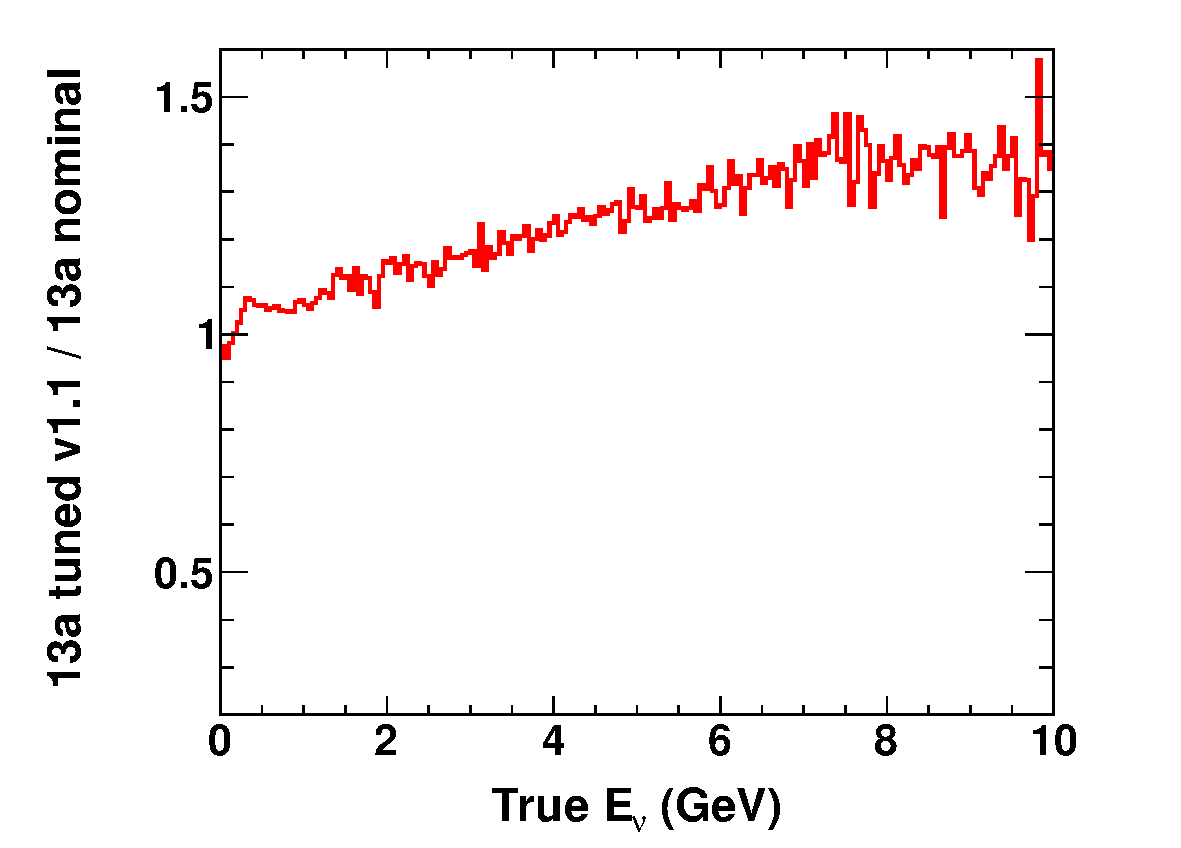
\includegraphics[width=18pc]{./joint_plots/spectrum_predictions/Flux/flux_ratio_13av1p1_to_13anom_numu_numode-eps-converted-to.pdf}
%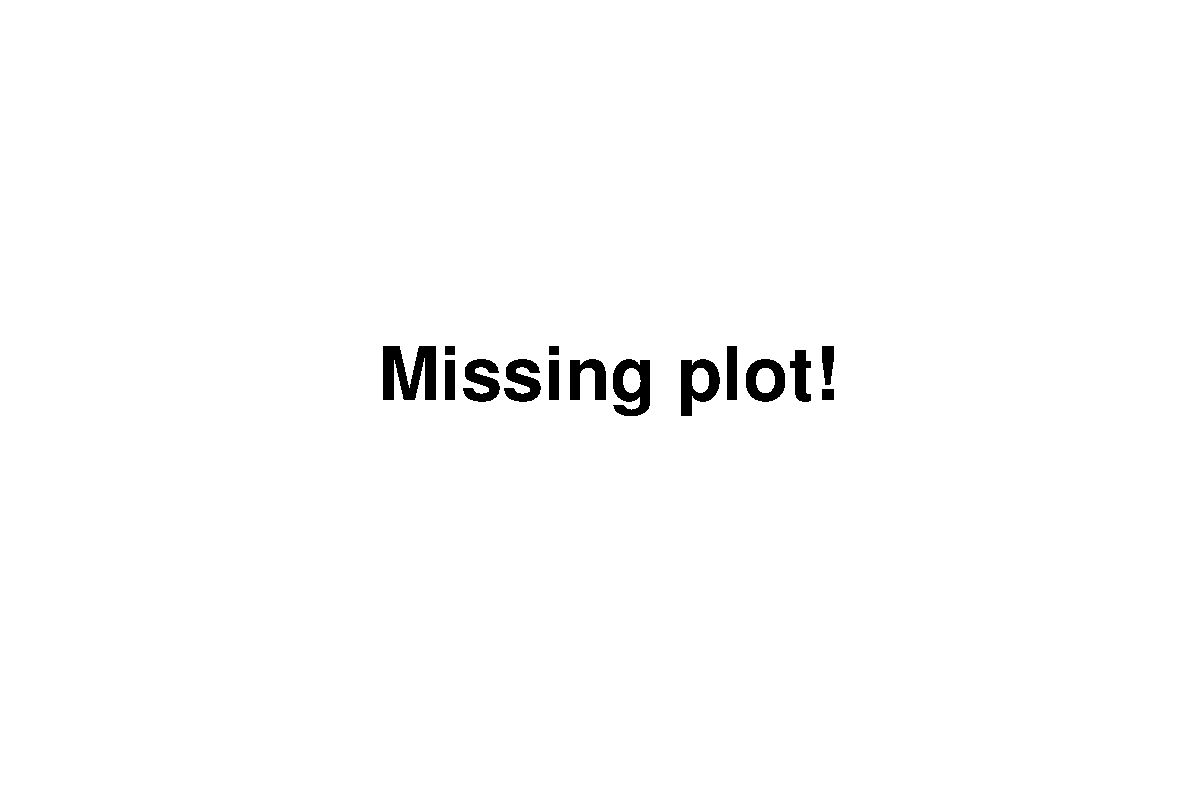
\includegraphics[width=18pc]{./images/missing_plot-eps-converted-to.pdf}
\caption {
  $\nu_\mu$ 13a\_v1.1 Run 1-6a flux tuning weights applied to nominal $\nu_\mu$ and oscillated-$\nu_e$ MC templates \cite{FluxTuning13a} (neutrino mode).
  }
\label{fig:na61_weights:numu_numode}
\end{minipage}
\hspace{0.06\linewidth}
\begin{minipage}[t]{0.48\linewidth}
\center
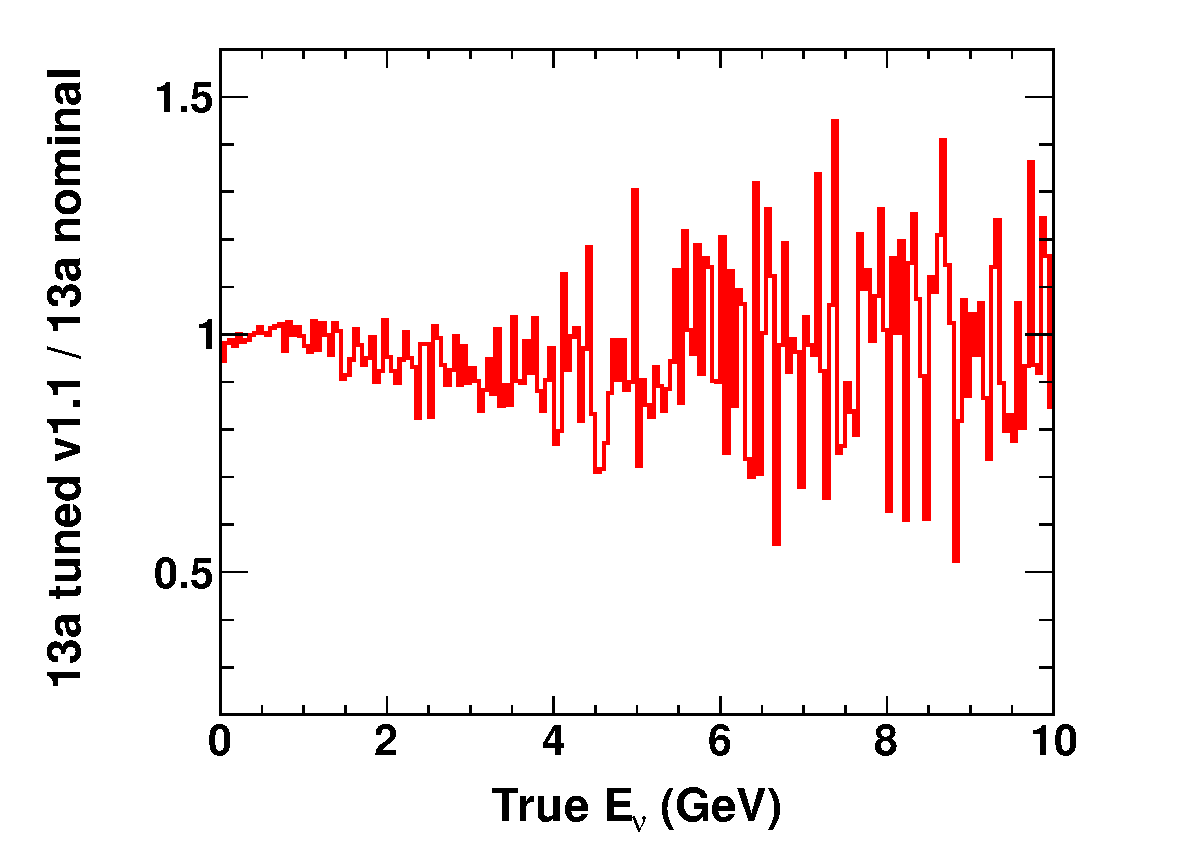
\includegraphics[width=18pc]{./joint_plots/spectrum_predictions/Flux/flux_ratio_13av1p1_to_13anom_numubar_numode-eps-converted-to.pdf}
%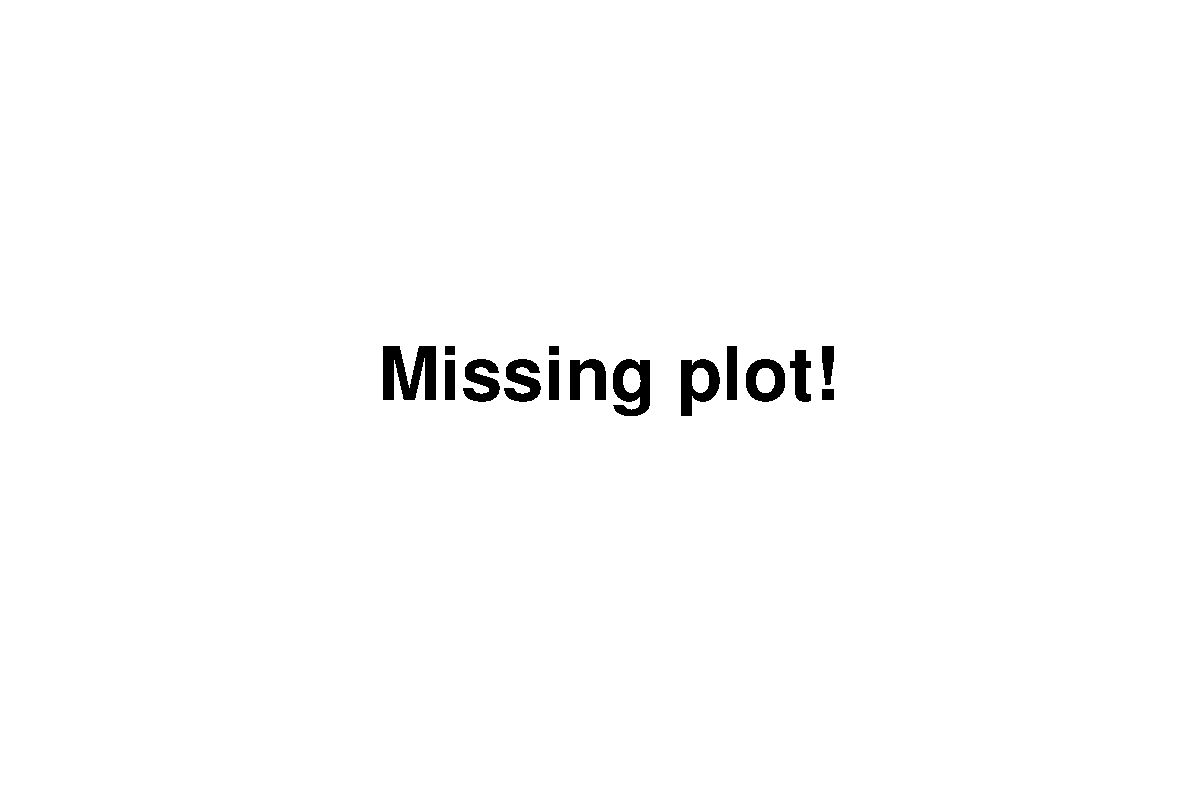
\includegraphics[width=18pc]{./images/missing_plot-eps-converted-to.pdf}
\caption {
  $\bar{\nu}_\mu$ 13a\_v1.1 Run 1-6a flux tuning weights applied to nominal $\bar{\nu}_\mu$ and oscillated-$\bar{\nu}_e$ MC templates \cite{FluxTuning13a} (neutrino mode).
}
\label{fig:na61_weights:numubar_numode}
\end{minipage}
\vfill
\begin{minipage}[t]{0.48\linewidth}
\center
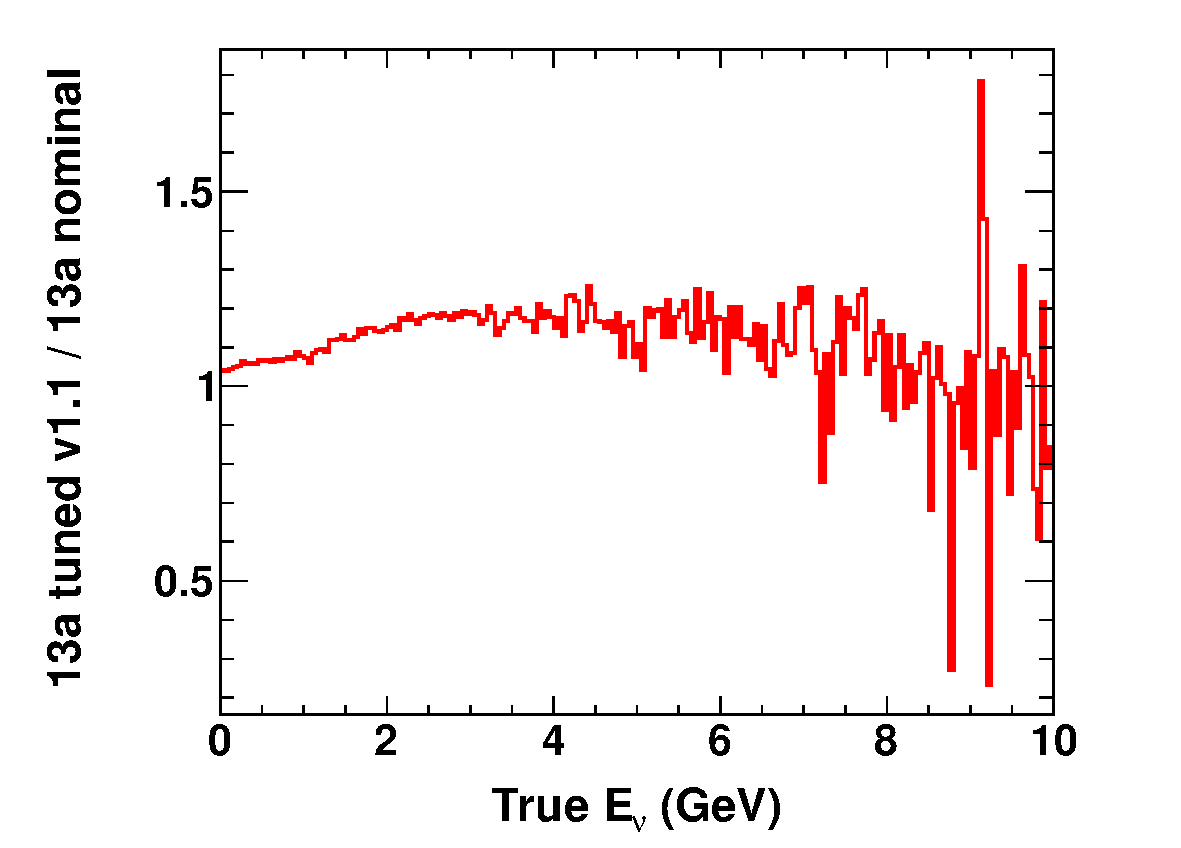
\includegraphics[width=18pc]{./joint_plots/spectrum_predictions/Flux/flux_ratio_13av1p1_to_13anom_nue_numode-eps-converted-to.pdf}
%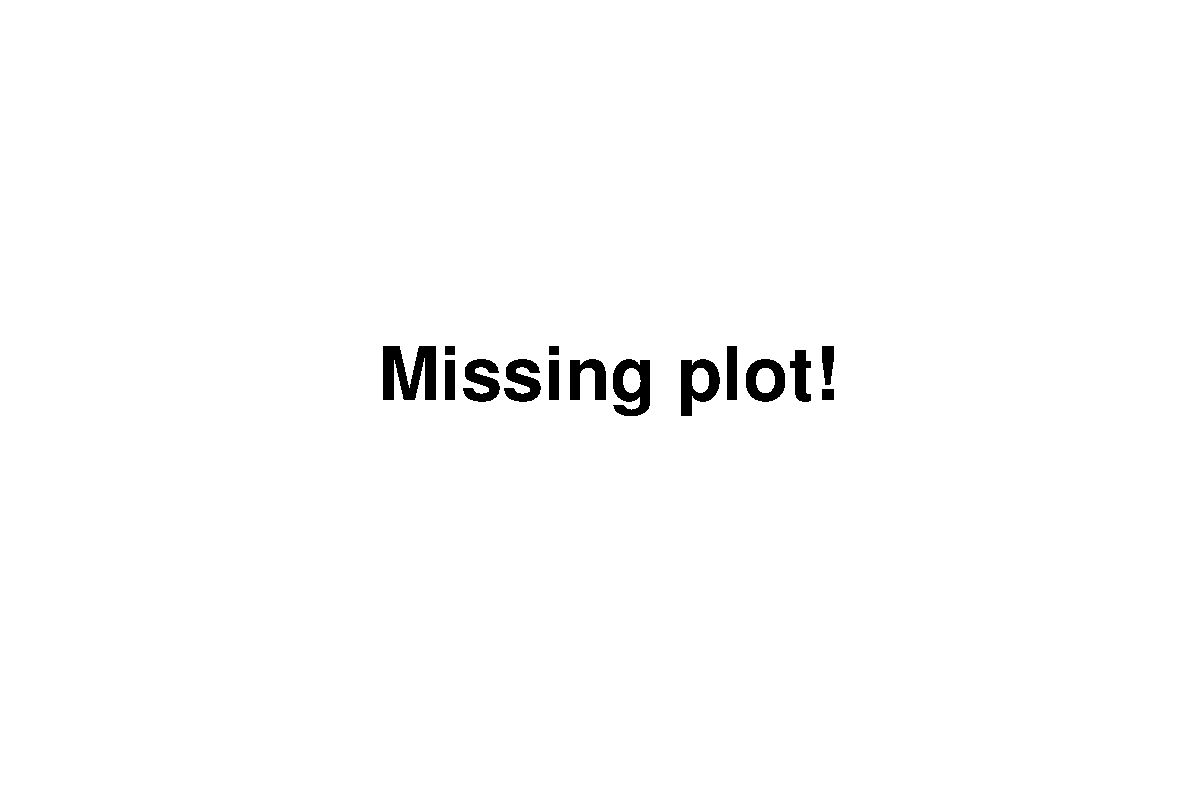
\includegraphics[width=18pc]{./images/missing_plot-eps-converted-to.pdf}
\caption {
  $\nu_e$ 13a\_v1.1\ Run 1-6a flux tuning weights applied to nominal $\nu_e$ MC templates \cite{FluxTuning13a} (neutrino mode).
}
\label{fig:na61_weights:nue_numode}
\end{minipage}
\hspace{0.06\linewidth}
\begin{minipage}[t]{0.48\linewidth}
\center
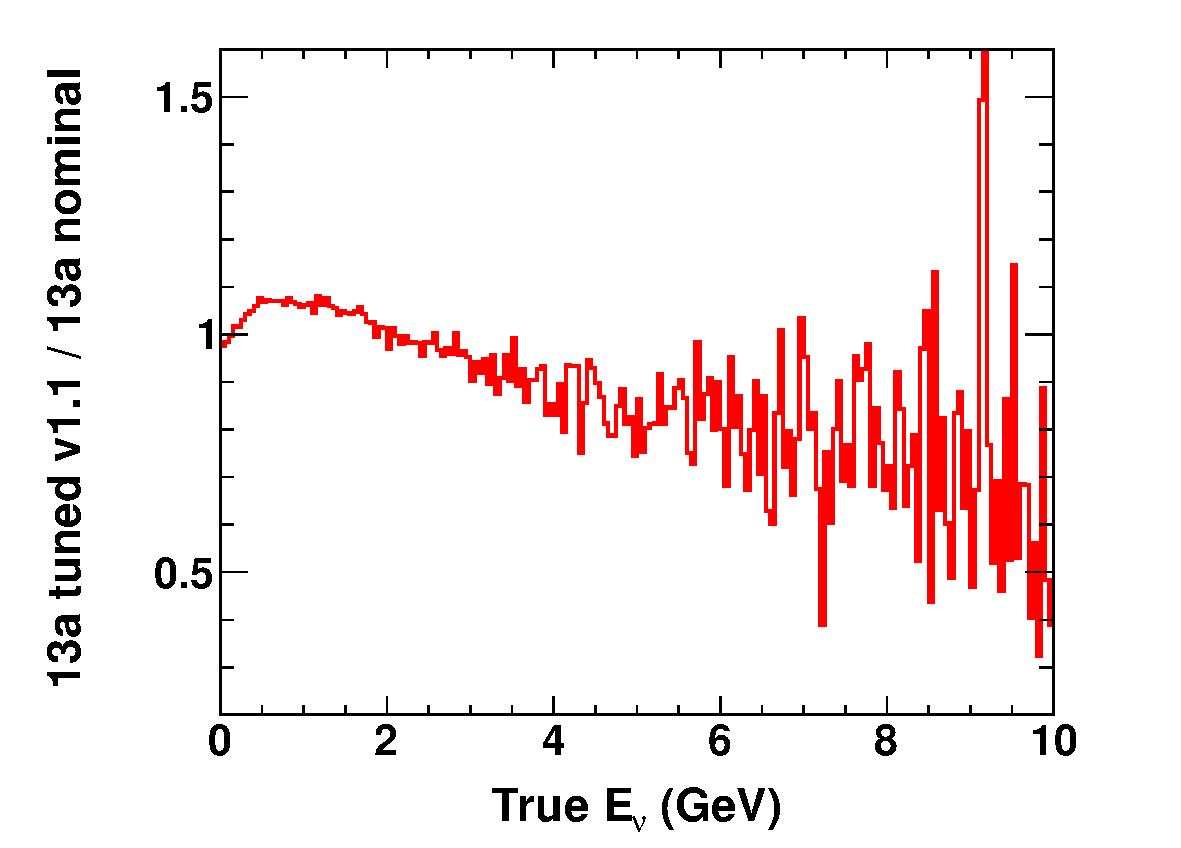
\includegraphics[width=18pc]{./joint_plots/spectrum_predictions/Flux/flux_ratio_13av1p1_to_13anom_nuebar_numode-eps-converted-to.pdf}
%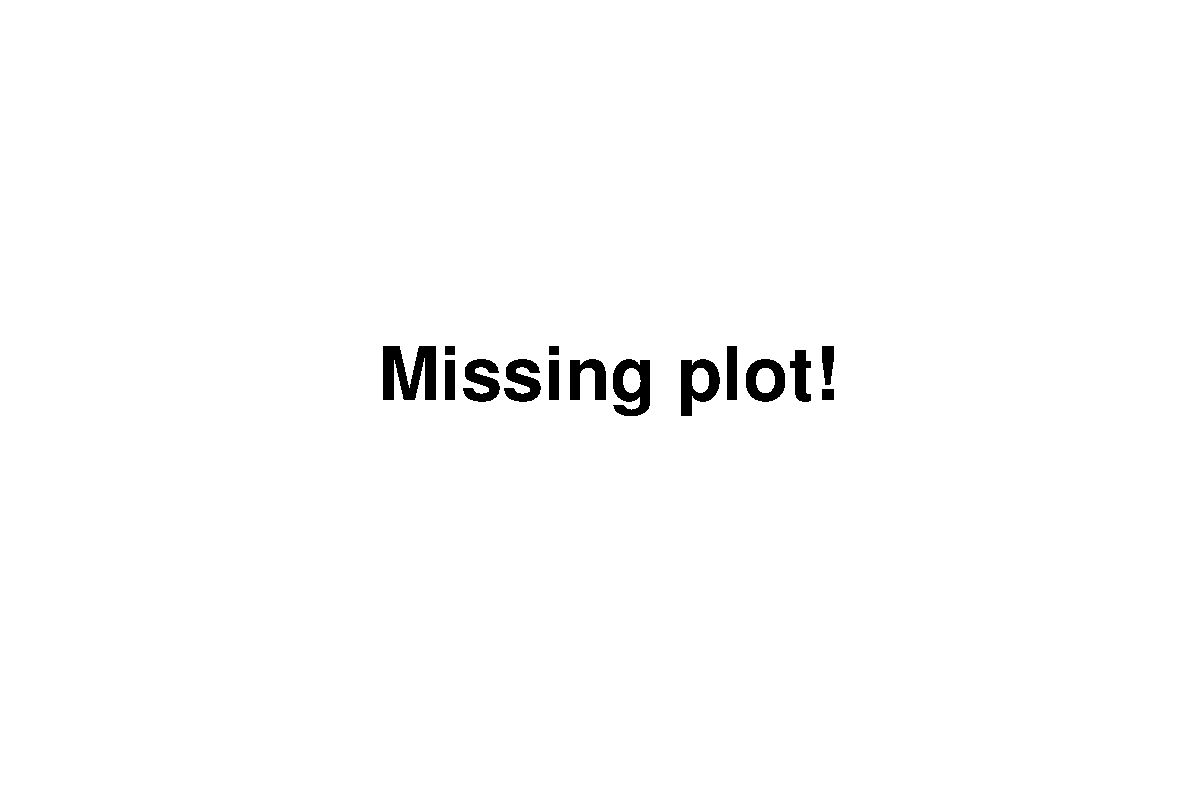
\includegraphics[width=18pc]{./images/missing_plot-eps-converted-to.pdf}
\caption {
  $\bar{\nu}_e$ 13a\_v1.1 Run 1-6a flux tuning weights applied to nominal $\bar{\nu}_e$ MC templates \cite{FluxTuning13a} (neutrino mode).
}
\label{fig:na61_weights:nuebar_numode}
\end{minipage}
\end{figure*}

%....................................................................................................................


\begin{figure*}[htb]
\begin{minipage}[t]{0.48\linewidth}
\center
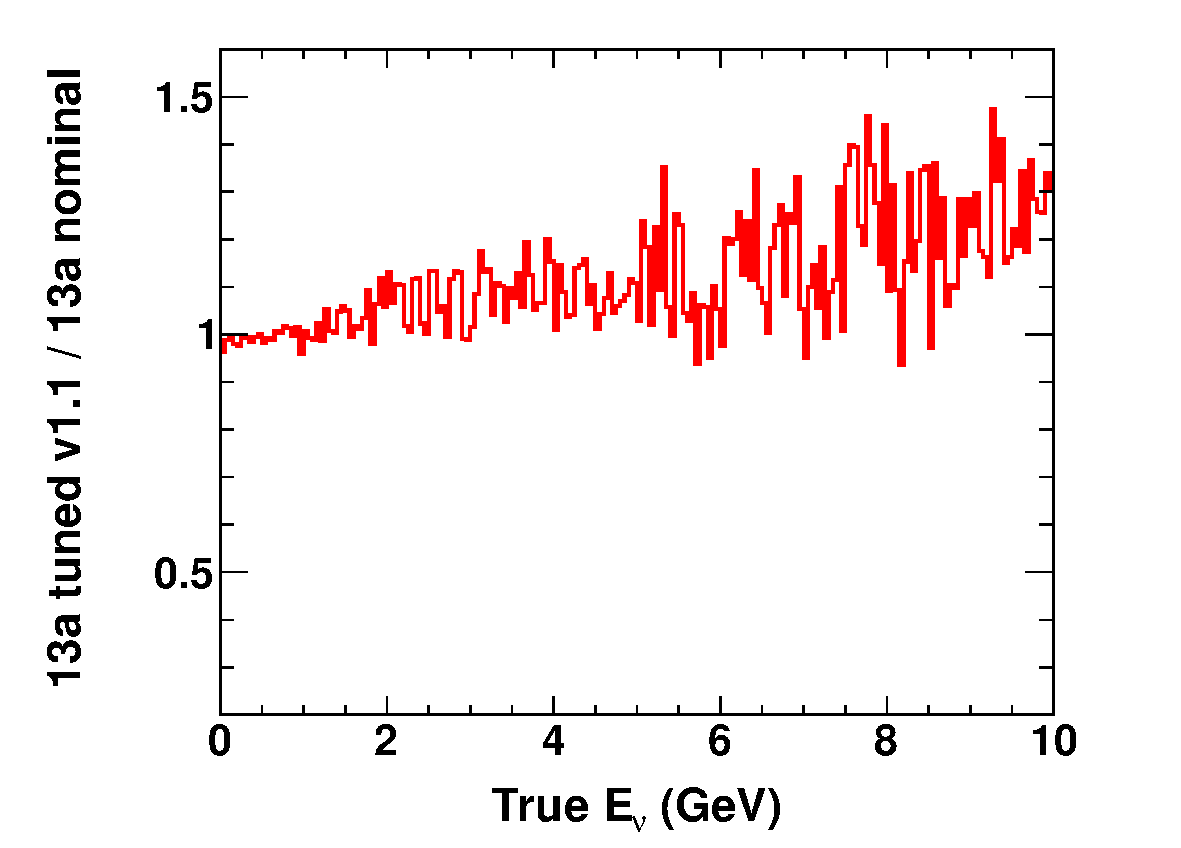
\includegraphics[width=18pc]{./joint_plots/spectrum_predictions/Flux/flux_ratio_13av1p1_to_13anom_numu_nubarmode-eps-converted-to.pdf}
%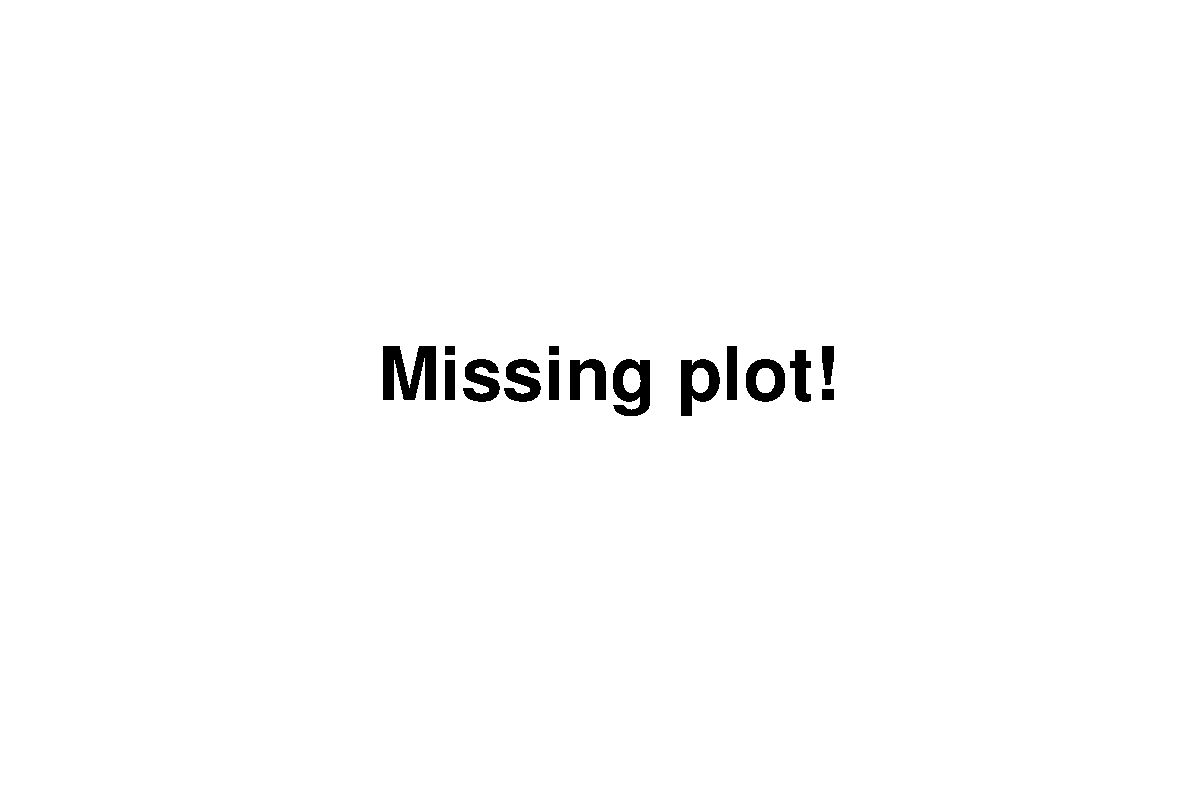
\includegraphics[width=18pc]{./images/missing_plot-eps-converted-to.pdf}
\caption {
  $\nu_\mu$ 13a\_v1.1 Run 5c-6b flux tuning weights applied to nominal $\nu_\mu$ and oscillated-$\nu_e$ MC templates \cite{FluxTuning13a} (antineutrino mode).
  }
\label{fig:na61_weights:numu_nubarmode}
\end{minipage}
\hspace{0.06\linewidth}
\begin{minipage}[t]{0.48\linewidth}
\center
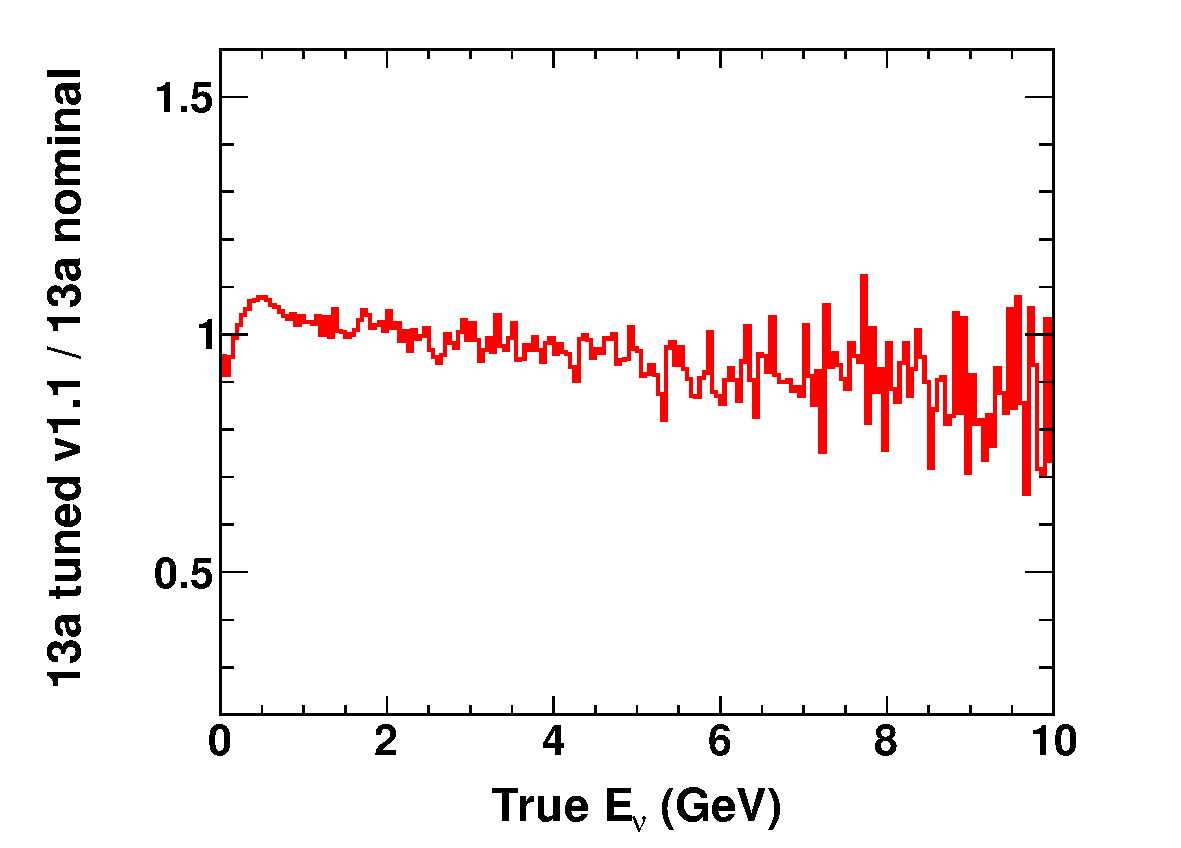
\includegraphics[width=18pc]{./joint_plots/spectrum_predictions/Flux/flux_ratio_13av1p1_to_13anom_numubar_nubarmode-eps-converted-to.pdf}
%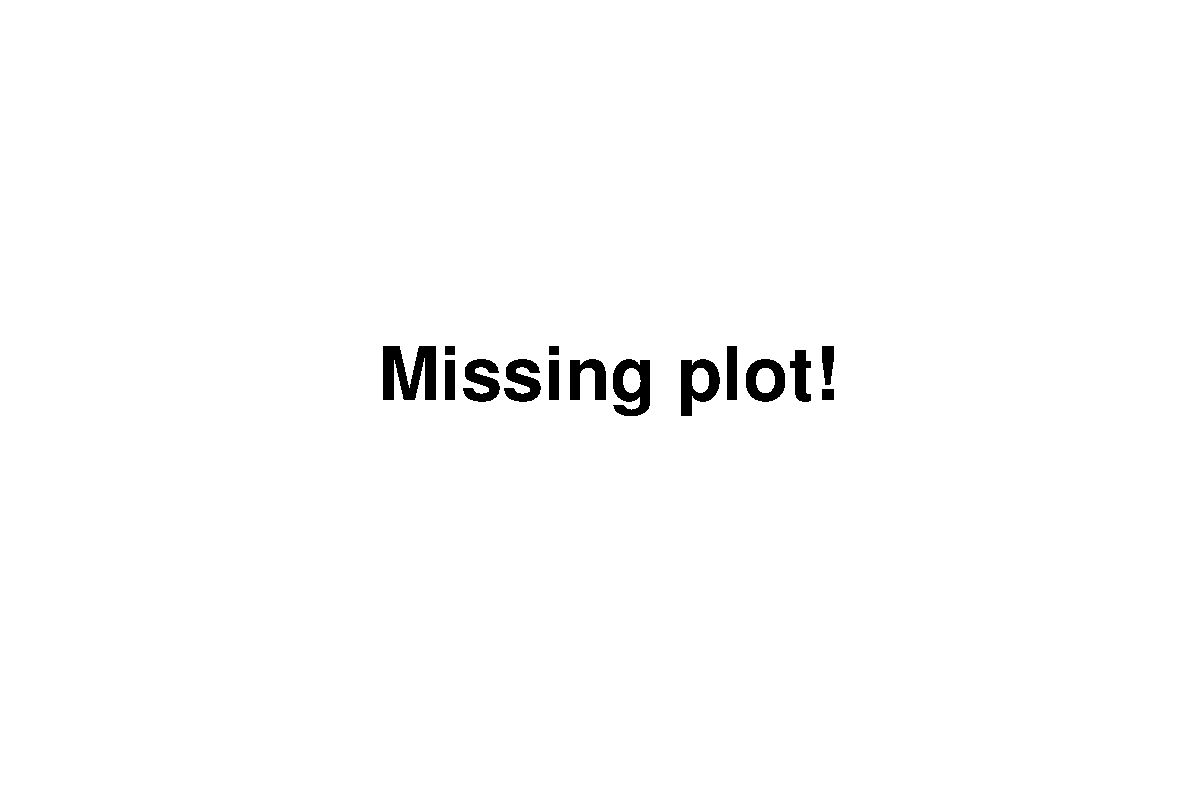
\includegraphics[width=18pc]{./images/missing_plot-eps-converted-to.pdf}
\caption {
  $\bar{\nu}_\mu$ 13a\_v1.1 Run 5c-6b flux tuning weights applied to nominal $\bar{\nu}_\mu$ and oscillated-$\bar{\nu}_e$ MC templates \cite{FluxTuning13a} (antineutrino mode).
}
\label{fig:na61_weights:numubar_nubarmode}
\end{minipage}
\vfill
\begin{minipage}[t]{0.48\linewidth}
\center
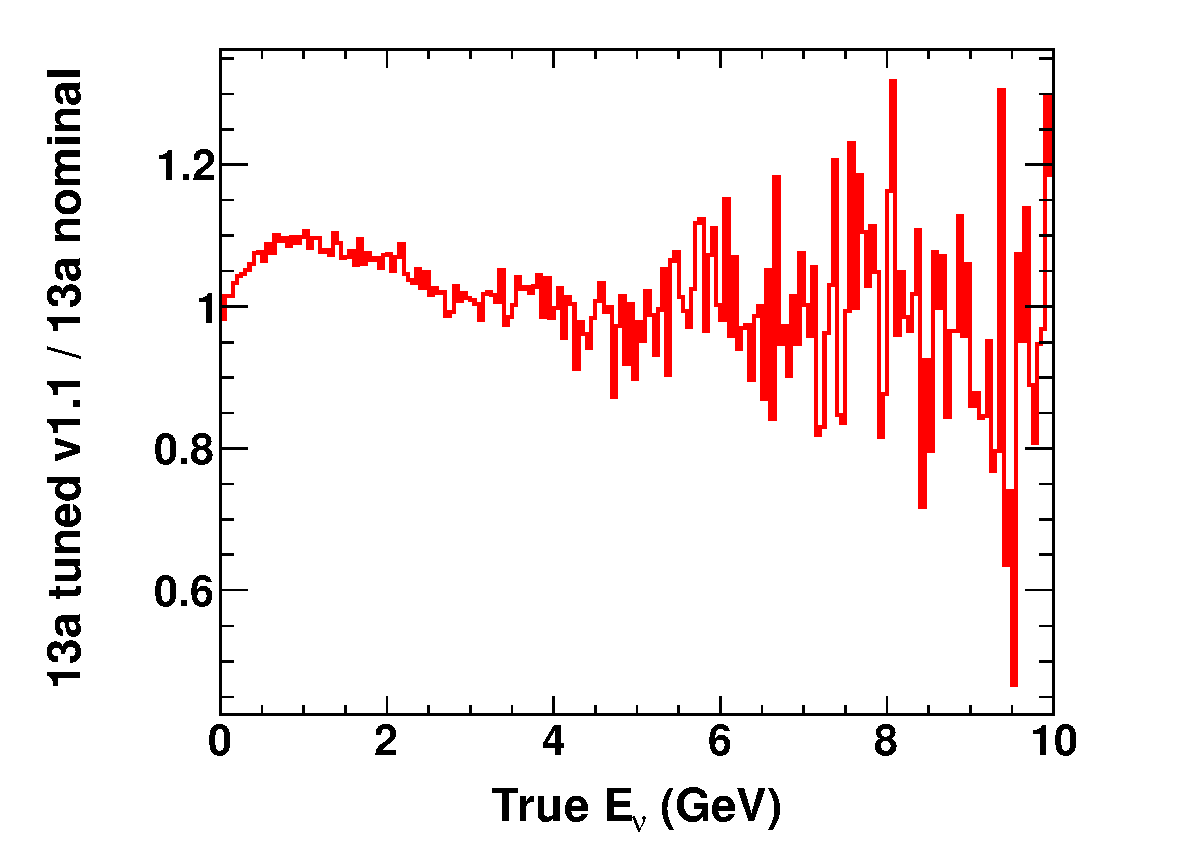
\includegraphics[width=18pc]{./joint_plots/spectrum_predictions/Flux/flux_ratio_13av1p1_to_13anom_nue_nubarmode-eps-converted-to.pdf}
%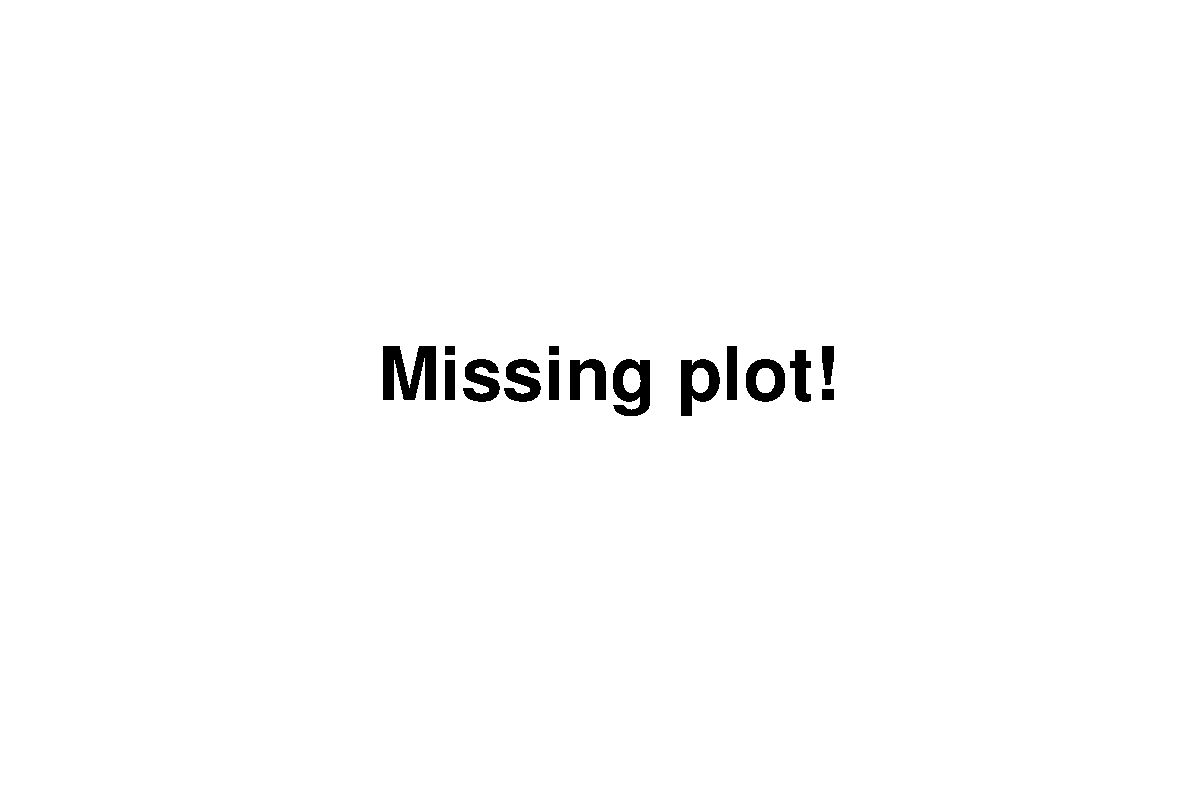
\includegraphics[width=18pc]{./images/missing_plot-eps-converted-to.pdf}
\caption {
  $\nu_e$ 13a\_v1.1\ Run 5c-6b flux tuning weights applied to nominal $\nu_e$ MC templates \cite{FluxTuning13a} (antineutrino mode).
}
\label{fig:na61_weights:nue_nubarmode}
\end{minipage}
\hspace{0.06\linewidth}
\begin{minipage}[t]{0.48\linewidth}
\center
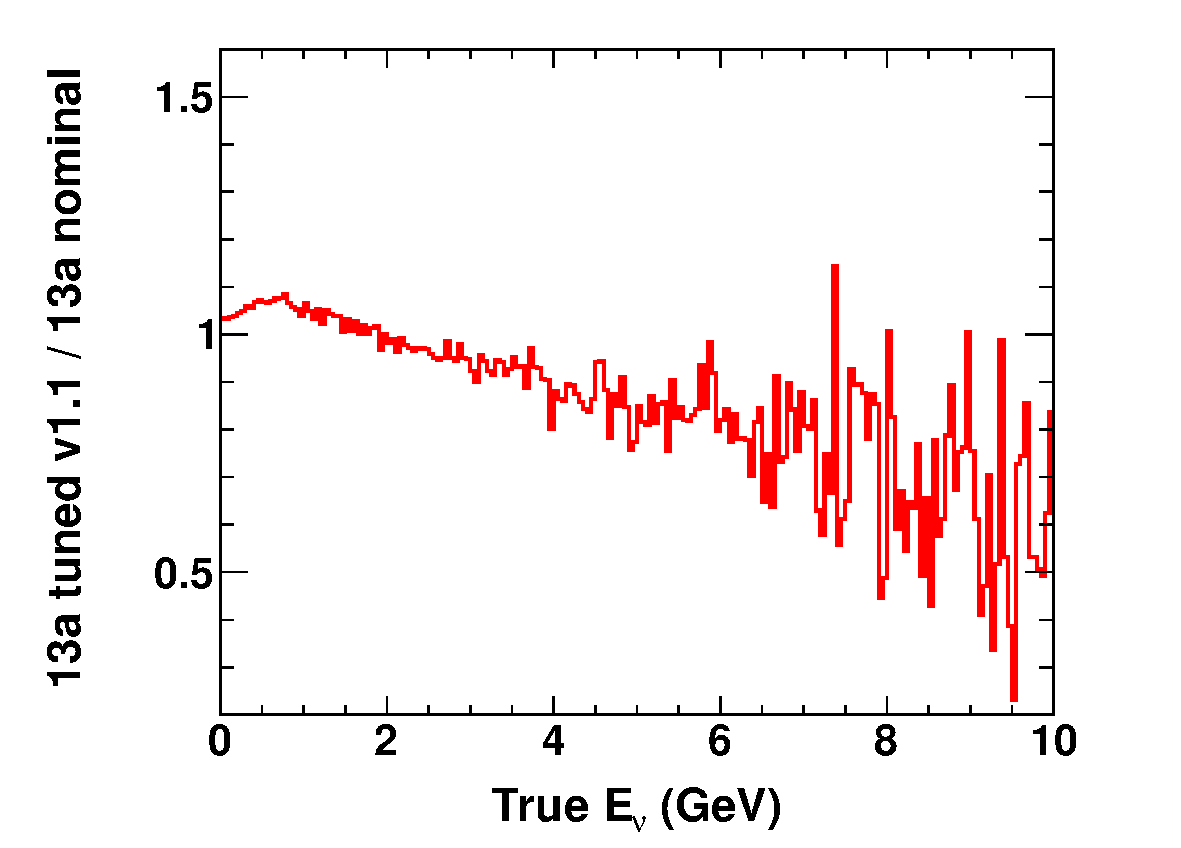
\includegraphics[width=18pc]{./joint_plots/spectrum_predictions/Flux/flux_ratio_13av1p1_to_13anom_nuebar_nubarmode-eps-converted-to.pdf}
%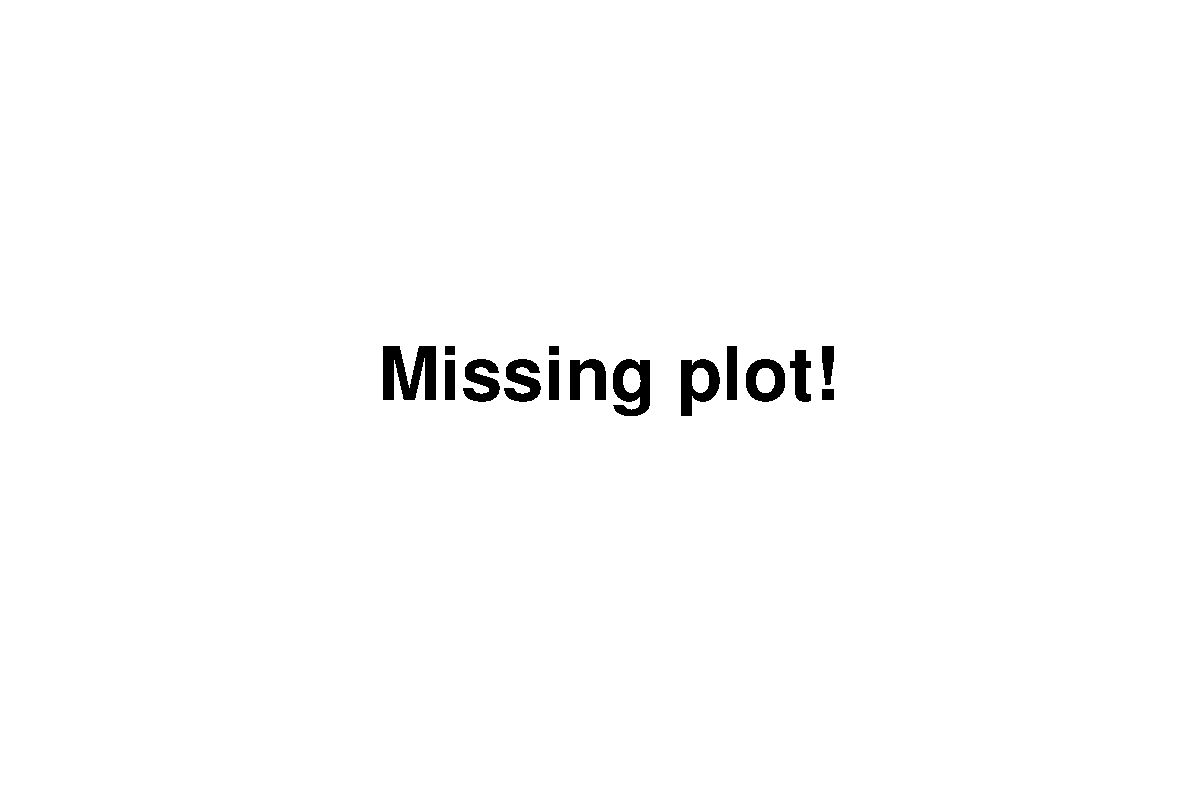
\includegraphics[width=18pc]{./images/missing_plot-eps-converted-to.pdf}
\caption {
  $\bar{\nu}_e$ 13a\_v1.1 Run 5c-6b flux tuning weights applied to nominal $\bar{\nu}_e$ MC templates \cite{FluxTuning13a} (antineutrino mode).
}
\label{fig:na61_weights:nuebar_nubarmode}
\end{minipage}
\end{figure*}

%....................................................................................................................
%....................................................................................................................

\subsection {Applying flux and cross section (BANFF) tuning based on ND280 data}
\label{sec:banff_weights}

The BANFF group has made a fit of the $\bar{\nu}_\mu$ and  $\nu_\mu$ 
%CC0$\pi$-like, CC1$\pi$-like and CC other 
ND280 samples 
to find the best-fit values of the flux normalisation and cross section parameters \cite{BANFF2015}. This 
analysis uses these best-fit values to reweight the NA61/SHINE-tuned MC templates, and the templates obtained after this second 
reweighting will be denoted the {\em BANFF-tuned} MC templates in this document.
A list of BANFF parameters, their best-fit values and their 1$\sigma$ prefit and postfit errors is given in 
\cref{tab:banff_uncertainties_flux_fhc},~\ref{tab:banff_uncertainties_flux_rhc} and
\ref{tab:banff_uncertainties_xsec}.

The effects of the BANFF tune on the predicted spectra is discussed 
in \cref{sec:nominal_and_tuned_predictions}. 
%(see \cref{fig:1Re_spectrum_w_and_wo_banff_weights} and \cref{tab:nsk_nominal_no_osc} and \cref{tab:nsk_nominal_osc}). 
%....................................................................................................................
%....................................................................................................................


\subsection{Applying neutrino oscillations}
\label{sec:applying_oscillations}

The MC templates are constructed from the unoscillated MC samples and must be weighted with the appropriate oscillation 
probability. Oscillations are applied as a function of true energy to the
%  $\bar{\nu}_{\mu}$ CCQE,
%  $\bar{\nu}_{\mu}$ CC1$\pi$,
%  $\bar{\nu}_{\mu}$ CC coherent,
%  $\bar{\nu}_{\mu}$ CC other,
%  $\nu_{\mu}$ CCQE,
%  $\nu_{\mu}$ CC1$\pi$,
%  $\nu_{\mu}$ CC coherent,
%  $\nu_{\mu}$ CC other,
%  $\bar{\nu}_{e}$ CCQE,
%  $\bar{\nu}_{e}$ CC1$\pi$,
%  $\bar{\nu}_{e}$ CC coherent,
%  $\bar{\nu}_{e}$ CC other
%  $\nu_{e}$ CCQE,
%  $\nu_{e}$ CC1$\pi$,
%  $\nu_{e}$ CC coherent,
%  $\nu_{e}$ CC other,
%  oscillated $\bar{\nu}_{\mu} \rightarrow \bar{\nu}_{e}$ CCQE,
%  oscillated $\bar{\nu}_{\mu} \rightarrow \bar{\nu}_{e}$ CC1$\pi$,
%  oscillated $\bar{\nu}_{\mu} \rightarrow \bar{\nu}_{e}$ CC coherent,
%  oscillated $\bar{\nu}_{\mu} \rightarrow \bar{\nu}_{e}$ CC other,
%  oscillated $\nu_{\mu} \rightarrow \nu_{e}$ CCQE,
%  oscillated $\nu_{\mu} \rightarrow \nu_{e}$ CC1$\pi$,
%  oscillated $\nu_{\mu} \rightarrow \nu_{e}$ CC coherent,
%  oscillated $\nu_{\mu} \rightarrow \nu_{e}$ CC other,
%  oscillated $\nu_{e} \rightarrow \nu_{\mu}$ CCQE,
%  oscillated $\nu_{e} \rightarrow \nu_{\mu}$ CC1$\pi$,
%  oscillated $\nu_{e} \rightarrow \nu_{\mu}$ CC coherent and
%  oscillated $\nu_{e} \rightarrow \nu_{\mu}$ CC other
  MC templates for all CC interactions.

The MC templates calculated from the
$\pbar{\nu}_{\mu}$ MC sample are weighted 
with P($\pbar{\nu}_{\mu} \rightarrow \pbar{\nu}_{\mu}$), with this survival probability being calculated using the 
oscillation parameters, namely $\sin^{2} \theta_{23}$, $\sin^{2} \theta_{12}$, $\sin^{2} \theta_{13}$, 
$|\Delta m^{2}_{32}|$ (normal hierarchy) or $|\Delta m^{2}_{31}|$ (inverted hierarchy), 
$\Delta m^{2}_{21}$ and $\delta_{CP}$. The $\pbar{\nu}_{e}$ templates are weighted with P($\pbar{\nu}_{e} \rightarrow \pbar{\nu}_{e}$), 
while the oscillated $\pbar{\nu}_{\mu} \rightarrow \pbar{\nu}_{e}$ templates are weighted with P($\pbar{\nu}_{\mu} \rightarrow \pbar{\nu}_{e}$) 
(the sample was generated assuming 100\% of $\pbar{\nu}_{\mu}$ transform to $\pbar{\nu}_{e}$). 
%The $\nu_{\mu}$ templates are weighted with P($\nu_{\mu}\rightarrow\nu_{\mu}$). 
%The $\nu_{e}$ templates are weighted with P($\nu_{e}\rightarrow\nu_{e}$) and the 
%oscillated $\nu_{\mu} \rightarrow \nu_{e}$ templates with P($\nu_{\mu}\rightarrow\nu_{e}$).
All these oscillation probabilities are computed in a 3-flavour framework including matter effects in constant-density matter
(assuming an Earth crust density of 2.6 g/cm$^{3}$).
Custom oscillation probability calculation code was developed within the {\em VALOR} analysis framework.
Details and estimates of the numerical accuracy of this code are first presented in \cite{OurRun12DisappAnalysis3Flavour},
and is also shown in Appendix A of \cite{OurRun123DisappAnalysis3Flavour}.
Comparisons between the {\em VALOR} oscillation probability calculation code and Prob3++ \cite{Prob3}, 
which is typically used by the alternative T2K oscillation analyses, are shown in Appendix B of \cite{OurRun123DisappAnalysis3Flavour}.

In the standard 3-flavour oscillation framework,
oscillations of $\pbar{\nu}_{e}$ and $\pbar{\nu}_{\mu}$ can yield $\pbar{\nu}_{\tau}$.
In this analysis, we neglect contributions from $\nu_{\tau}$-CC and $\bar{\nu}_{\tau}$-CC as their
energy threshold is around 3.5 GeV and their effect is negligible\footnote{
A back-of-the-envelope calculation can be found in the replies to
comments and revision history document of
\cite{OurRun123DisappAnalysis3Flavour} that gives $\ll 1\%$ $\nu_\tau$
contamination in the 1-ring $\mu$-like Super-K sample. A Super-K MC study is required
to determine whether the Super-K efficiency assumptions made there are valid.
  }.
Accordingly, this analysis uses no $\nu_{\tau}$-CC and $\bar{\nu}_{\tau}$-CC MC templates
(and, in fact, no $\nu_{\tau}$ and $\bar{\nu}_{\tau}$ Super-K MC samples are available).

It should be emphasized here that
the $\nu_{\mu}$ NC MC templates for a mode $m$ contain the
NC MC templates for the mixture of $\nu_{e}$+$\nu_{\mu}$+$\nu_{\tau}$ resulting from
3-flavour $\nu_{\mu}$ oscillations for that mode $m$. The same applies to the $\bar{\nu}_{\mu}$, $\nu_{e}$ and $\bar{\nu}_{e}$ 
NC MC templates. These NC MC templates are unchanged under standard 3-flavour oscillations.% (see also \cref{sec:}).

Also it should be noted that there are no explicit NC MC templates made from the oscillated $\bar{\nu}_{e}$ and $\nu_{e}$ 
samples. If they were used, the oscillated $\bar{\nu}_{e}$ (i.e.\ $\bar{\nu}_{e}$ coming from oscillations of $\bar{\nu}_{\mu}$) 
would be double counted since they are already included in the $\bar{\nu}_{\mu}$ NC MC templates. The same applies to oscillated 
$\nu_{e}$.

%....................................................................................................................
%....................................................................................................................

\subsection {Predictions of nominal and tuned-MC spectra}
\label{sec:nominal_and_tuned_predictions}

In this section, we present the expected spectra in Super-K for various oscillation scenarios. 
%We also present estimates of the effect of the NA61/SHINE and BANFF tunings and of assumptions 
%made in the 3-flavour neutrino oscillation framework used in this analysis. 
Unless explicitly stated otherwise, the oscillation 
parameters are set to the Asimov data set A shown in \cref{tab:osc_params_joint_asimov} and the normal mass hierarchy is assumed.
All plots are generated for an integrated exposure 
corresponding to Run 1-7c.
%of \TotalPotNu{} POT for neutrino and \TotalPotNuBar{} POT for antineutrino mode.


Predicted single ring Super-K spectra are shown in \cref{fig:joint_ereco_vs_theta_all}. 
By comparing neutrino and antineutrino mode $e$-like plots it is clear that $E_{reco}$ vs $\theta$ distributions are differently populated
by $\nu_{\mu} \rightarrow \nu_e$ and $\bar{\nu}_{\mu} \rightarrow \bar{\nu}_e$ events.
\textbf{More details on the advantage of the 2-dimensional templates are given in appendix~\ref{app:templates_elike}.}

%for oscillations assuming the normal hierarchy and the oscillation parameters shown in \cref{tab:osc_params_joint}.

\begin{figure*}[htb]
\center
\begin{subfigure}[b]{0.49\textwidth}
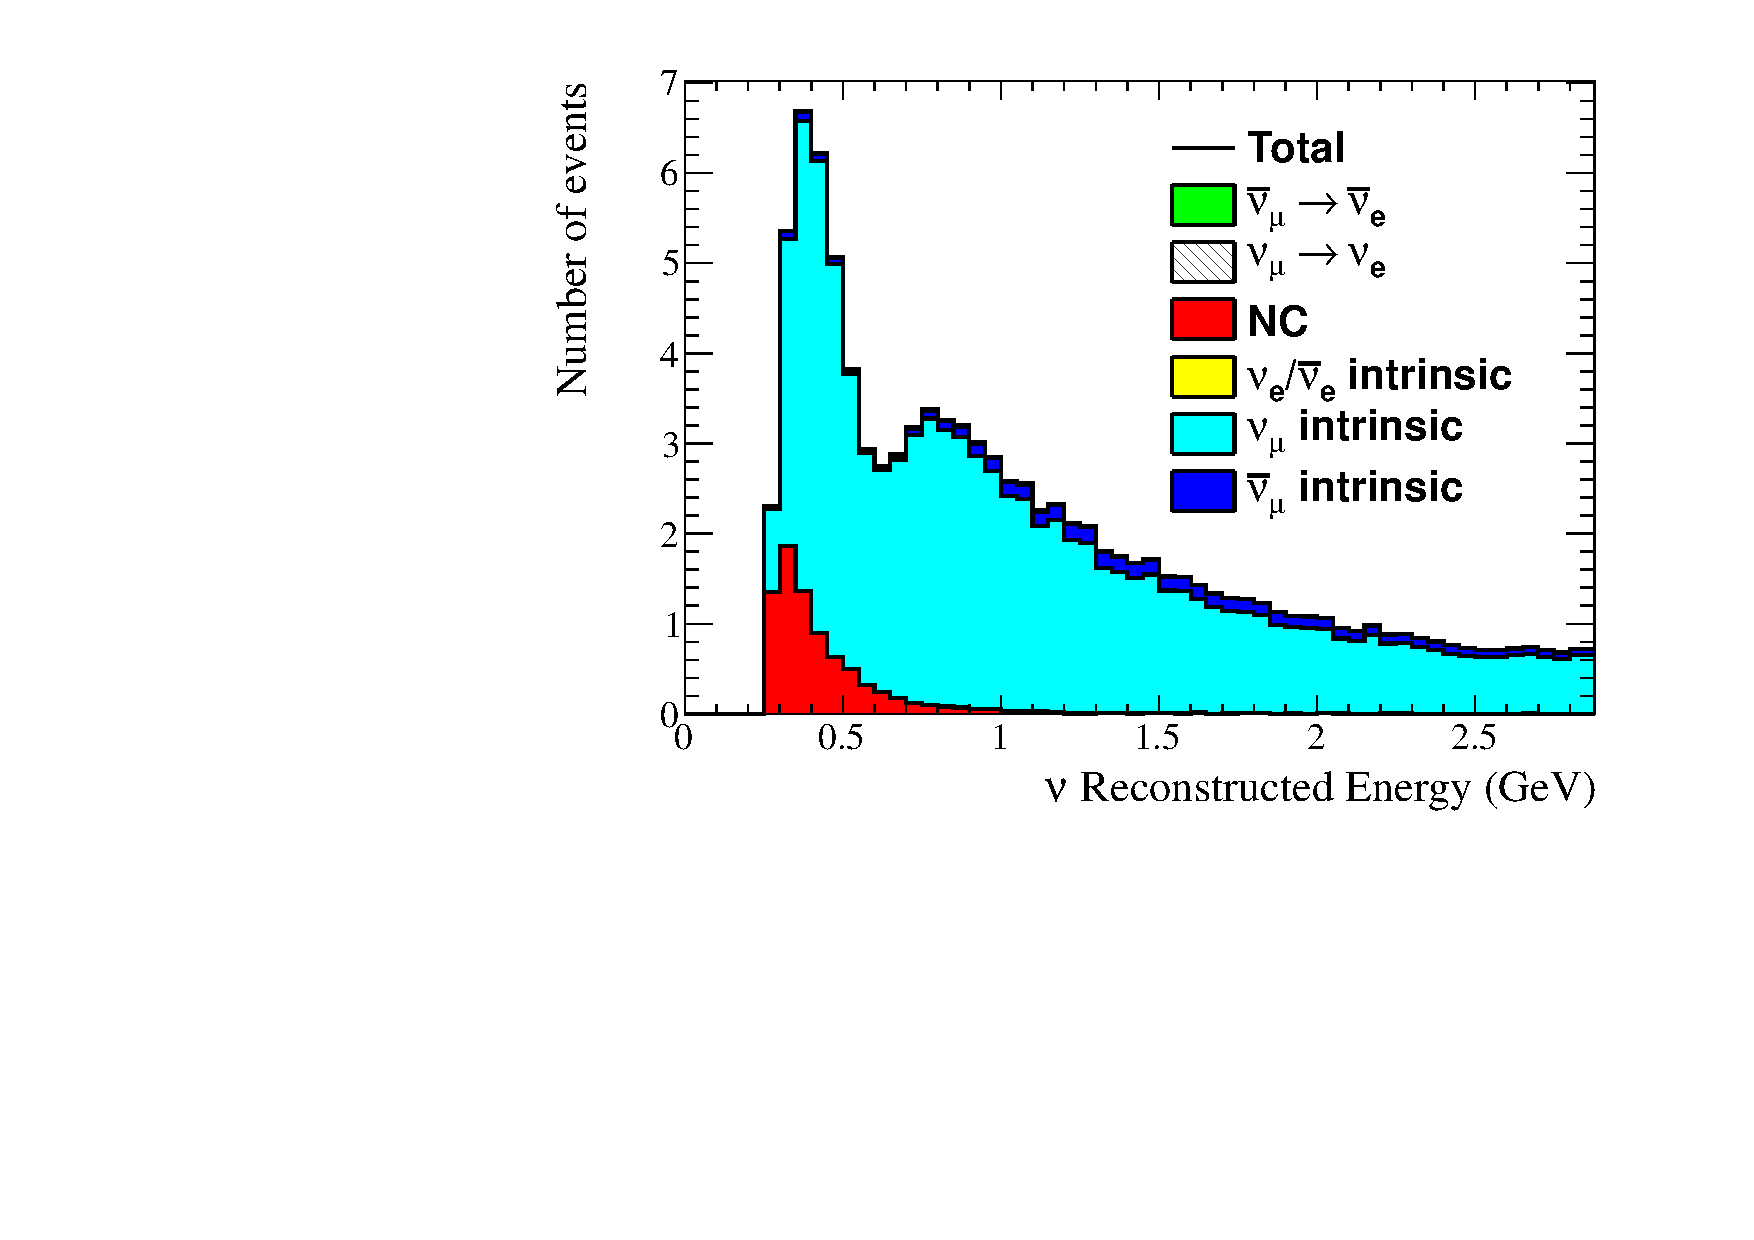
\includegraphics[width=0.9\textwidth]{joint_plots/spectrum_predictions/template_ereco_1rmu_zoom.pdf}
\caption{Muon-like, neutrino mode}
\end{subfigure}
\begin{subfigure}[b]{0.49\textwidth}
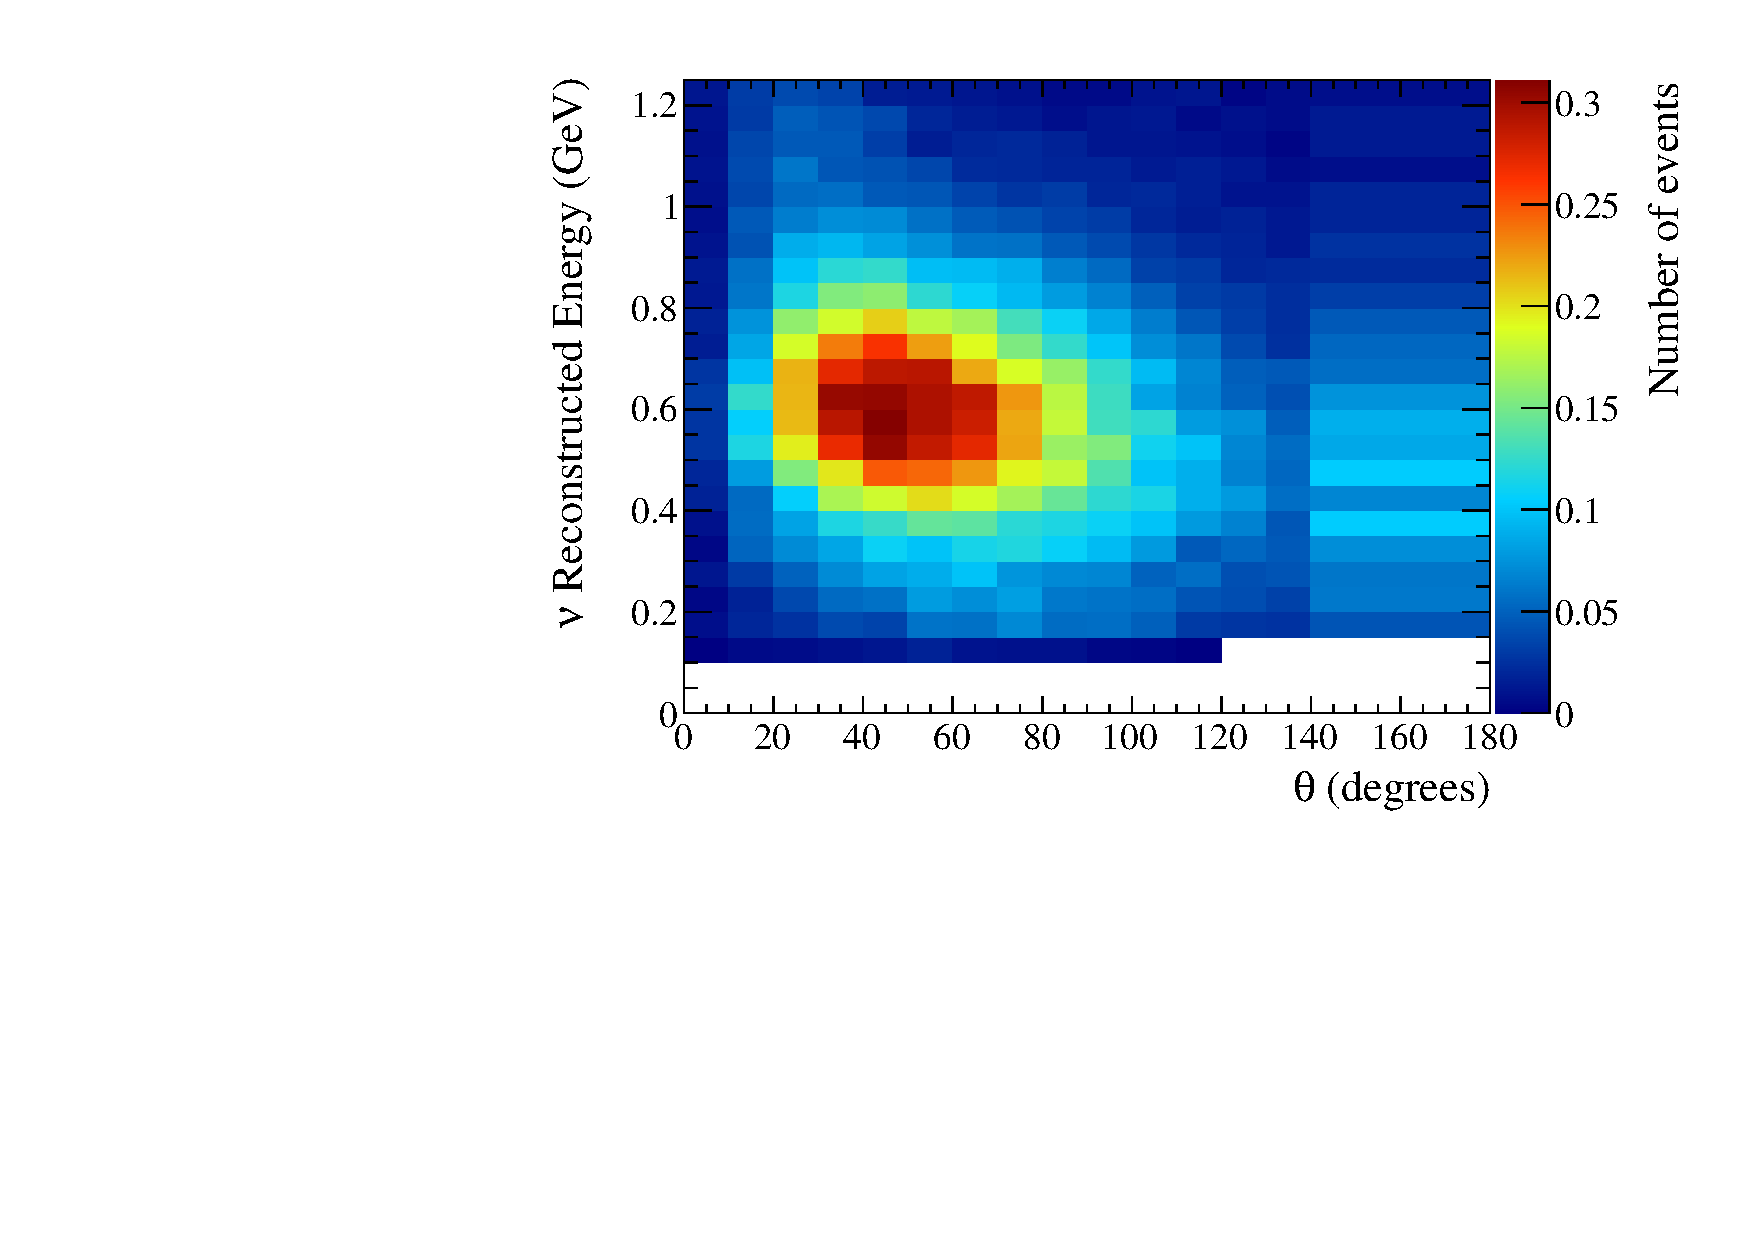
\includegraphics[width=0.9\textwidth]{joint_plots/spectrum_predictions/template_ereco_vs_theta_tot_1re.pdf}
\caption{Electron-like, neutrino mode}
\end{subfigure}
\begin{subfigure}[b]{0.49\textwidth}
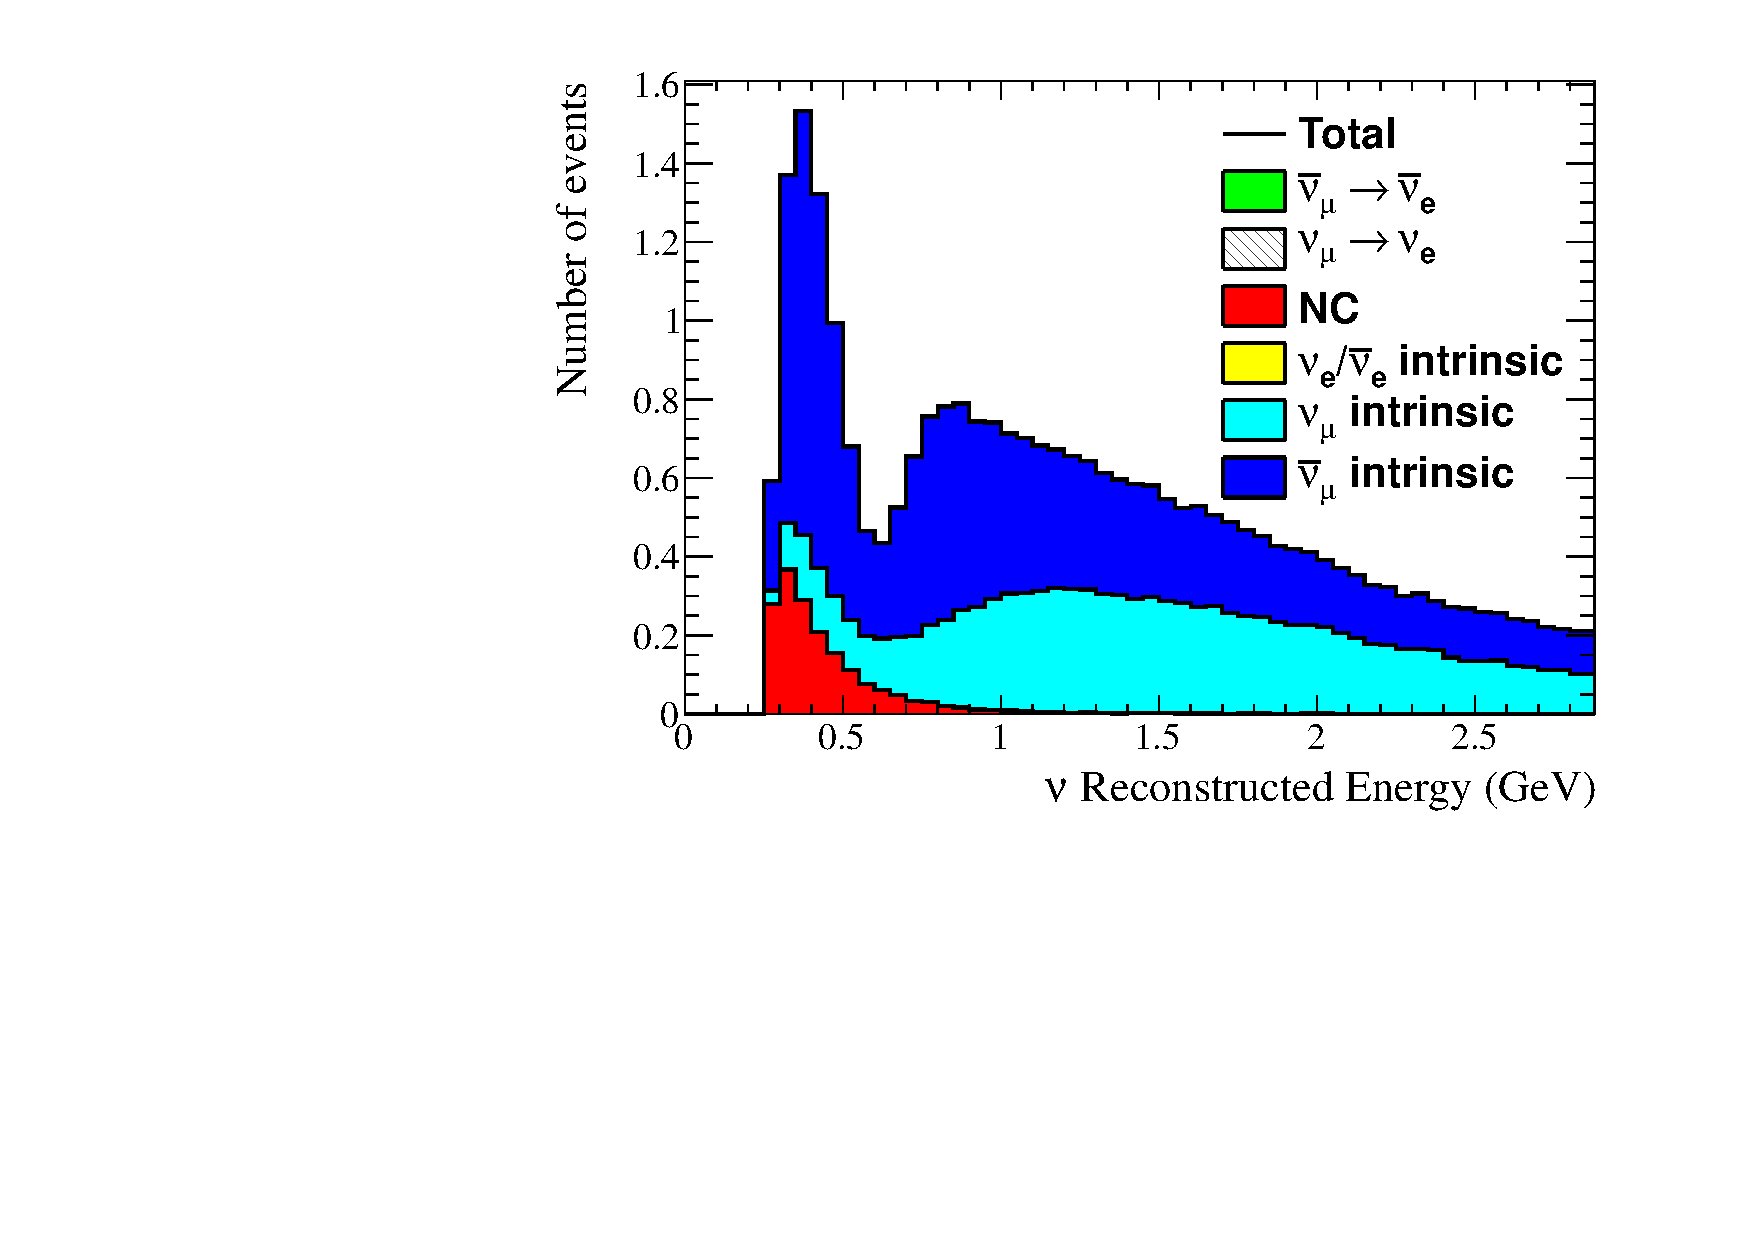
\includegraphics[width=0.9\textwidth]{joint_plots/spectrum_predictions/template_ereco_rhc1rmu_zoom.pdf}
\caption{Muon-like, antineutrino mode}
\end{subfigure}
\begin{subfigure}[b]{0.49\textwidth}
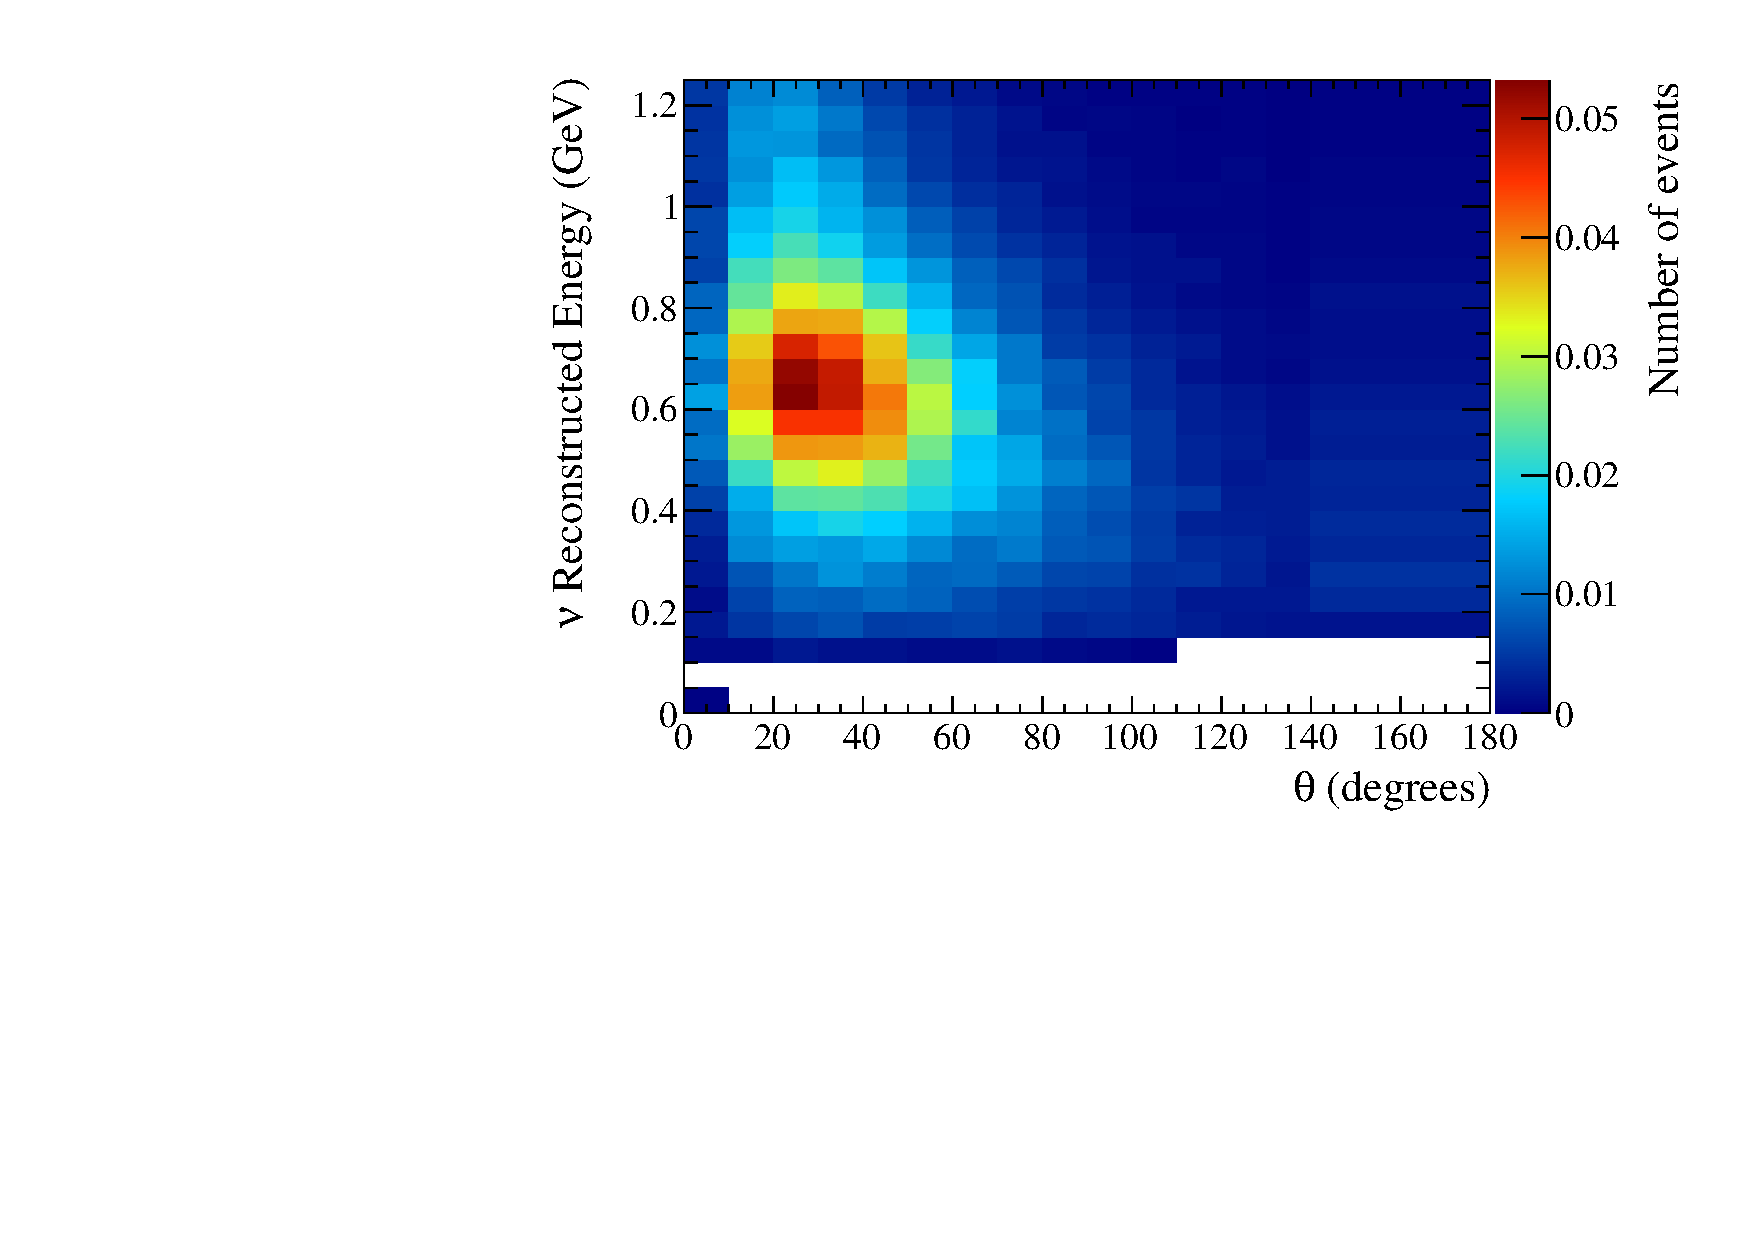
\includegraphics[width=0.9\textwidth]{joint_plots/spectrum_predictions/template_ereco_vs_theta_tot_rhc1re.pdf}
\caption{Electron-like antineutrino mode}
\end{subfigure}
\begin{subfigure}[b]{0.49\textwidth}
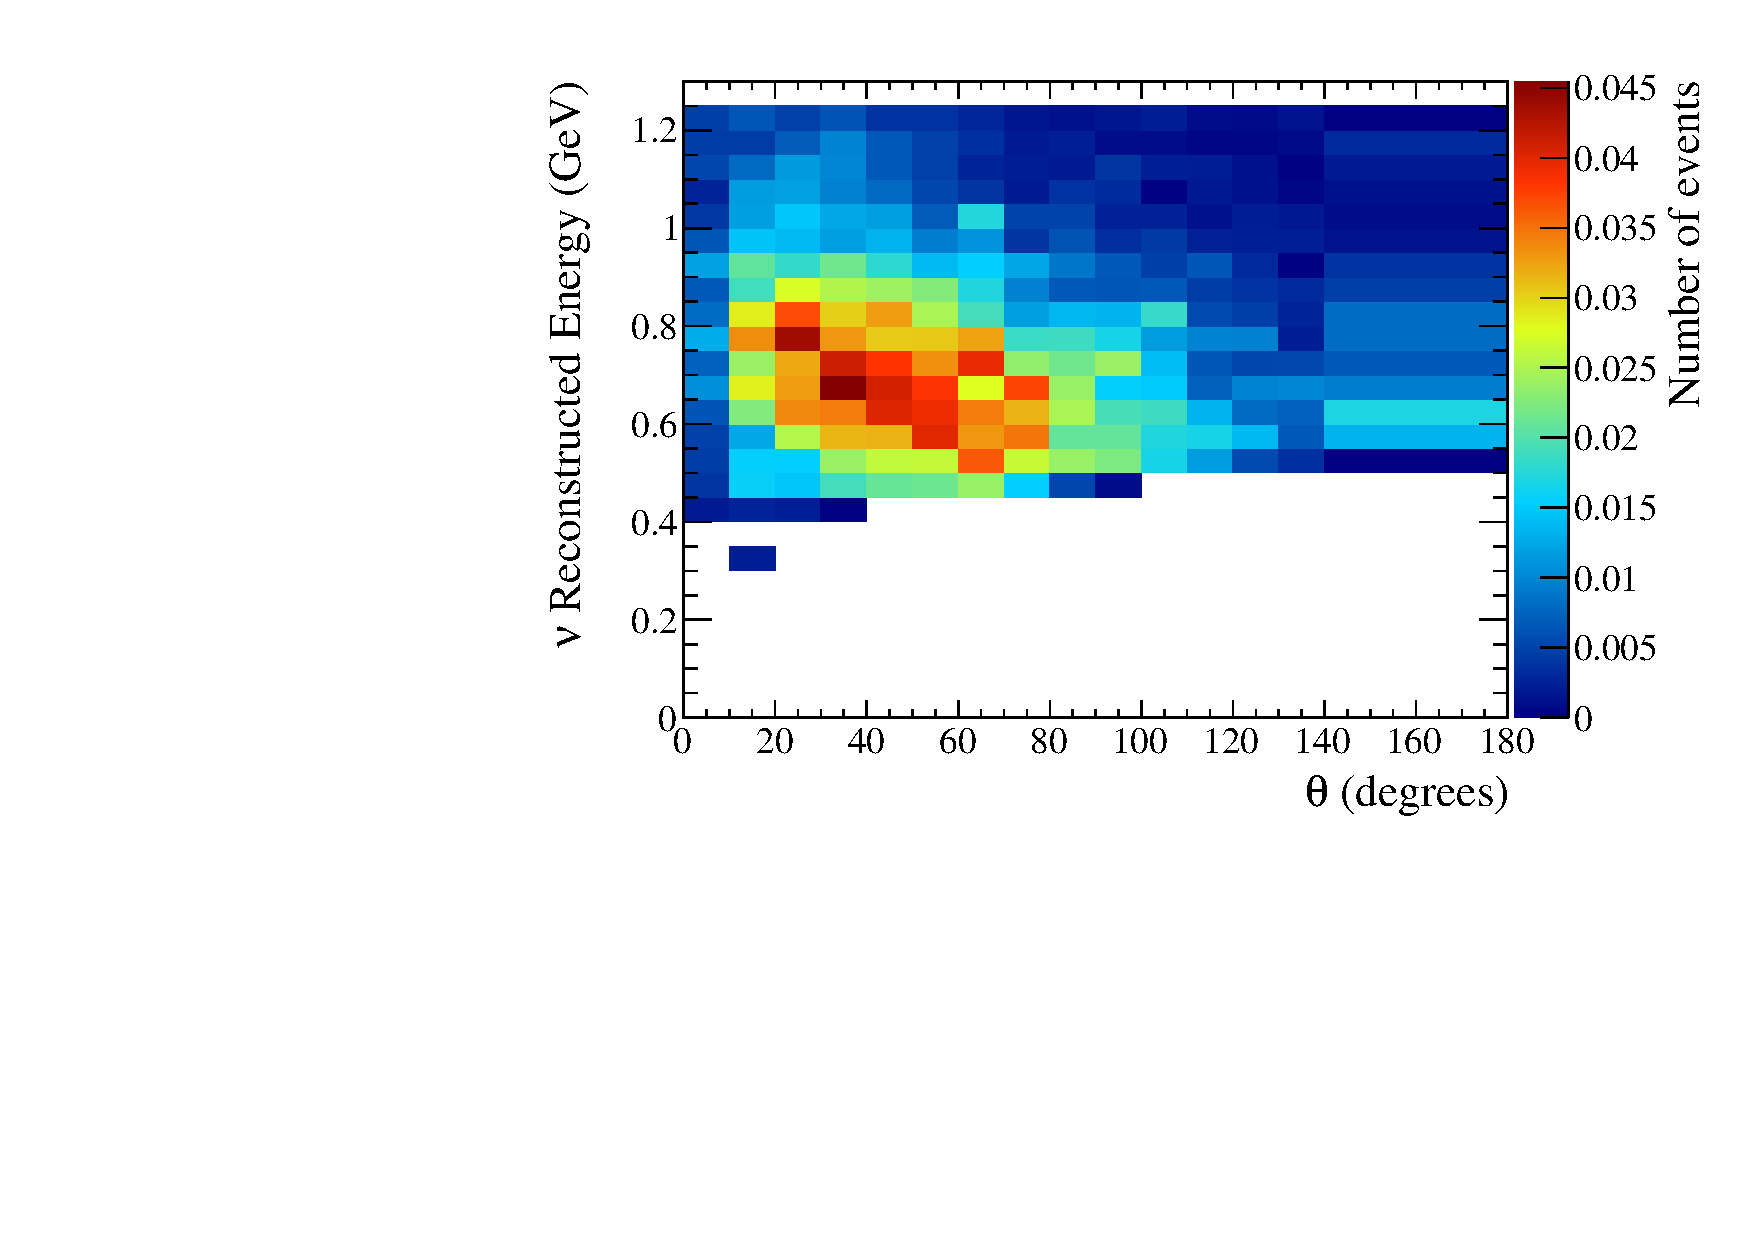
\includegraphics[width=0.9\textwidth]{joint_plots/spectrum_predictions/template_theta_ccpi.pdf}
\caption{\nueCConepi-like, neutrino mode}
\end{subfigure}
\caption {
Predicted spectra, muon-like distributions are function of the reconstructed neutrino energy,
while the electron-like, including \nueCConepi, distributions are function of both the reconstructed neutrino energy and
the reconstructed angle between the outgoing lepton and the neutrino direction.
The distributions correspond to the statistics collected in the full Run 1-7c data set.
%for an exposure 
%of $6.914 \times 10^{20}$ POT in neutrino mode
%and
%of $4.011 \times 10^{20}$ POT in antineutrino mode.
The muon-like distributions are broken down by the following components:
$\bar{\nu}_{\mu} \to \bar{\nu}_e$ (green), 
$\nu_{\mu} \to \nu_e$ (black/white), 
NC (red),
$\nu_e + \bar{\nu}_e$ intrinsic beam (yellow),
$\nu_{\mu}$ intrinsic beam (light blue)
and
$\bar{\nu}_{\mu}$ intrinsic beam (blue).
The spectra are generated with the systematic parameters measured with the ND280 data 
shown in 
\cref{tab:banff_uncertainties_flux_fhc},~\ref{tab:banff_uncertainties_flux_rhc},
\ref{tab:banff_uncertainties_xsec} and the nominal Super-K systematic parameters shown in ~\cref{tab:banff_uncertainties_skdetfsi}
and the oscillation parameters corresponding to the Asimov data set A 
shown in \cref{tab:osc_params_joint_asimov}.
}
\label{fig:joint_ereco_vs_theta_all}
\end{figure*}















%A MC tune derived using NA61/SHINE data is applied to the nominal MC templates, and another tune derived using the ND280 data is 
%applied to the NA61/SHINE-tuned templates as described in \cref{sec:na61_weights} and \cref{sec:banff_weights}.
%%
%The fractional difference in the expected number of single $e$-like ring events when switching from the nominal MC to the
%NA61/SHINE-tuned MC templates is shown in \cref{fig:1Re_spectrum_w_and_wo_na61_weights} 
%both oscillated and not oscillated. 
%%In \cref{fig:1Re_spectrum_w_and_wo_banff_weights} it is shown the fractional difference in the expected number of
%%single-ring $e$-like events when switching from the NA61/SHINE-tuned MC templates to the BANFF-tuned MC templates.
%In \cref{fig:1Re_spectrum_w_and_wo_na61_weights} it is shown the fractional difference in the expected number of single-ring e-like events
%when switching from the nominal MC templates to NA61/SHINE-tuned MC templates.
%%
%The effects of the NA61/SHINE and BANFF tunes on the total expected number of single-ring $e$-like events
%and on the numbers in each of the \NMCTemplate{} component interaction modes are shown in
%\cref{tab:nsk_nominal_no_osc} for no oscillations, and in
%\cref{tab:nsk_nominal_osc} for oscillations assuming the normal hierarchy, and the oscillation parameters shown in \cref{tab:osc_params_fixed_values_reactor}.
%Finally, the effects of the NA61/SHINE and BANFF tunes on the reconstructed energy spectrum of
%single $e$-like ring events are shown in
%\cref{fig:1Re_spectrum_w_and_wo_banff_weights}.
%In each case, spectra are shown for both no oscillations and for oscillations assuming the normal hierarchy, and the oscillation parameters shown in \cref{tab:osc_params_fixed_values_reactor}.
%%Also shown are the ratio of flux-tuned spectrum to nominal spectrum, and
%%BANFF-tuned spectrum to flux-tuned spectrum in \cref{fig:1Re_spectrum_w_and_wo_banff_weights}.
%Also shown are the ratio of BANFF-tuned spectrum to flux-tuned spectrum in \cref{fig:1Re_spectrum_w_and_wo_banff_weights}.

%%% Local Variables:
%%% mode: latex
%%% TeX-master: "jointfit_5sample2016"
%%% End:

\clearpage

\section {Systematic effects in the prediction of the single $\mu$-like ring event energy spectrum}
\label{sec:systematics}

%....................................................................................................................
%....................................................................................................................

\subsection {Input systematic parameters}
\label{sec:systematics:inputs}

This analysis considers \NSyst{} flux, cross section and Super-K detector systematic parameters 
plus 7 oscillation parameters, which can be treated as either systematic parameters or
as parameters of interest, depending on the analysis that is performed.

\begin{enumerate}

\item 
{\bf Flux and cross-section parameters} (65 parameters).\\

In this analysis, all the flux and cross-section systematic parameters are included in the ND280 data (BANFF) fit.
However, since ND280 is not sensitive to the electron neutrino cross section and the NC1$\gamma$ parameters they remain unconstrained
The parameters fit are 
11 $\nu_{\mu}$, 5 $\bar{\nu}_{\mu}$, 7 $\nu_{e}$ and 2 $\bar{\nu}_{e}$ neutrino mode (FHC) flux parameters, 
5 $\nu_{\mu}$, 11 $\bar{\nu}_{\mu}$, 2 $\nu_{e}$ and 7 $\bar{\nu}_{e}$ antineutrino mode (RHC) flux parameters 
and 15 cross-section parameters. 
Best-fit values of these parameters and a covariance matrix giving their correlated uncertainties are obtained by the BANFF group from a fit 
of the $\bar{\nu}_\mu$ and $\nu_\mu$ 
%CC0$\pi$-like, CC1$\pi$-like and CC other-like 
ND280 samples as described in Ref~\cite{BANFF2015}. 
A list of the BANFF parameters, their best-fit values and their prefit and postfit errors,
taken from TN-230 \cite{BANFF2016},
is given in 
\cref{tab:banff_uncertainties_flux_fhc},~\cref{tab:banff_uncertainties_flux_rhc},
\cref{tab:banff_uncertainties_xsec}.

The best-fit values are used to reweight the templates as described in \cref{sec:banff_weights}, and the
postfit errors in the covariance matrix are used as prior uncertainties in this analysis.  The Super-K
systematic parameters are shown in \cref{tab:banff_uncertainties_skdetfsi}.  All the cross section parameters
set to 1 correspond to the NEUT nominal value, except ``CC other shape'' for which the NEUT nominal value is
0.  For all the normalisation parameters, 1 is the nominal pre-banff fit value.

The effects of these correlated uncertainties are evaluated using the Cholesky method, that allows throws of
the systematic parameters according to their multivariate distribution taking into account existing
correlations.
%The covariance matrix is ``Cholesky decomposed'' 
%into the product of a lower triangular matrix (all elements above the diagonal are zero) and its transpose (in which all elements below the 
%diagonal are zero). Random tweaks of each parameter are independently drawn from a Gaussian distribution with mean zero and standard deviation 1, 
%and these random numbers are put into a vector. This vector is then multiplied by the lower triangular matrix to give a vector of tweaked 
%uncertainties that have the correct correlations between them. The BANFF parameters are then varied by these tweaked uncertainties, with all 
%parameters being varied simultaneously. This process may be repeated as many times as necessary. 

Some of the cross-section parameters have complicated, often non-linear, effects on true and reconstructed
neutrino energy bin normalisations; the effects of uncertainties in these parameters are evaluated by
reweighting the MC templates. Weights are calculated for tweaks from -3$\sigma$ to +3$\sigma$ in steps of
0.5$\sigma$, and interpolations are made between those weights using cubic splines (for MaQE only, weights are
calculated from -7$\sigma$ to +3$\sigma$). Cubic splines are made for the following cross-section
uncertainties:
\begin{itemize}
\item CCQE axial-mass scaling factor (MaQE)
\item Fermi momentum for $^{16}$O
\item Binding energy for $^{16}$O
\item Nucleon to $\Delta$ transition axial form factor (C$^{A}_{5}$) 
\item Resonance-production axial-mass scaling factor (MaRes)
\item Scale of isospin 1/2 nonresonant background
\item CC other shape
\end{itemize}
The splines are made in bins of theta, true and reconstructed energy, and the binning is given in Ref.\
\cite{splineinfo}. The $\theta$ binning is the same as for the analysis templates, shown in
\cref{sec:mc_templates:template_binning}.

The effects of the flux and cross-section normalisation uncertainties are also evaluated by reweighting the MC
templates, but no splines are made for them since the weight is identical to the tweak for these uncertainties
(each flux parameter is a normalisation for a limited range of true energy).  The cross section parameters
which simply normalise the overall spectrum component are:
\begin{itemize}
\item 2p-2h, applied to all the 2p-2h events (both neutrino and antineutrino)
\item 2p-2h-$\bar{\nu}$, applied to all the antineutrino 2p-2h events
\item CC coherent for $^{16}$O normalisation
\item NC coherent normalisation
\item NC other normalisation
\item NC $1\gamma$ normalisation
\item CC $\nu_{e}$ normalisation
\item CC $\bar{\nu}_{e}$ normalisation
\end{itemize}

Uncertainties due to ``second class currents" are implemented as an additional uncertainty on CC
$\bar{\nu}_{e}$ and CC $\nu_{e}$ parameters with a 2\% anti-correlated constraint between them.  The BANFF
parameters are applied to the MC templates as specified in appendix~\ref{app:systematics} in
\cref{tab:apply_syst_to_template_mulike_fhc,%
  tab:apply_syst_to_template_elike_fhc,%
  tab:apply_syst_to_template_mulike_rhc,%
  tab:apply_syst_to_template_elike_rhc}
%      tab:apply_syst_to_template_nueCConepi_fhc }.
The normalisation parameter of the NC$1\gamma$ component was not used in the previous analyses,
since it was included in NC other.

In the BANFF fit a bias on the best-fit flux parameters is present due to the degeneracy between the neutrino
flux and ND280 detector parameters.  For this reason a covariance matrix that accounts for the bias of the
flux as well as all the other parameters is summed in quadrature with the total post-fit covariance. Furthermore
the best-fit values have been corrected in order to remove the bias. A full description of the procedure is
given in \cite{BANFF2015}.  As shown in \cite{OurRun1617b17cJointAnalysis3Flavour} the impact of the bias on the
systematic parameters fitted by the BANFF analysis is small compared to the other systematic uncertainties.


%....................................................................................................................

\subsection {Comparison of predicted number of events in neutrino mode $e$-like sample between current and 2015 analysis}
\label{sec:systematics:comparison_events_elike_2015}

The predicted number of events in antineutrino mode $e$-like sample is now smaller compared to the
$\bar{\nu}_e$ appearance analysis presented at the 2015 summer conferences
\cite{OurRun56AntiNueBarAppearanceAnalysis3Flavour}, 3.218 instead of 3.729.  The differences between the
current and previous oscillation analyses are mainly due to:

\begin{enumerate}

\item new value of $\sin^2 \theta_{13}$ corresponding to the PDG 2015 release, as shown in
  \cref{tab:osc_params_joint_asimov}, which is 0.0217 while in the previous analysis it was 0.0250. If the old
  PDG value is used the expected number of antineutrino mode $e$-like events becomes 3.542.

\item Subsequently, if the cross section parameters are set to the old post-BANFF fit values, the expected
  number of events becomes 3.63. Indeed all the post-BANFF 2015 fit cross section parameters are higher
  compared to the 2016 BANFF fit result. The effect of the flux parameters is smaller, indeed if they are set
  to BANFF 2015 result, the expected number of events becomes 3.66.
 
\item Finally, after all the changes listed above, if the rescaling of CC coherent and NC$1\gamma$ components
  (see \cref{sec:mc_templates:input_mc}) is not applied, agreement between the 2015 and 2016 analysis is
  obtained. The first one increases the number of events up to 3.772 while the latter one reduces down to
  3.711, which is approximately the number of events expected in the 2015 analysis.

%\item the total normalisation for 2p-2h events for antineutrinos is 0.894,   �  
%	where the BANFF best-fit of the 2p-2h parameter applied only to $\bar{\nu}$ is $0.578$ and 
%	the best-fit of the 2p-2h parameter applied to all the flavors is 1.546.
%	 This reduces the expected total number 
%	of $\bar{\nu}_e$ events, while in the past analysis a single systematic parameter was applied to all the 2p-2h events 
%	and its BANFF best-fit was about 1.031.

\end{enumerate}


{
\renewcommand{\arraystretch}{1.2}
\begin{table}
\centering
\begin{tabular}{| c | c | c | c |}
\hline
           Parameter & Description & Best fit & 1$\sigma$ pre/postfit \\
           & & & fractional error \\
\hline
            0 &  $\nu_{\mu}$ flux normalisation, E = 0.0 - 0.7 GeV               & 1.142   & 0.094 / 0.071 \\ 
            1 &  $\nu_{\mu}$ flux normalisation, E = 0.7 - 1.0 GeV               & 1.091   & 0.079 / 0.053 \\ 
            2 &  $\nu_{\mu}$ flux normalisation, E = 1.0 - 1.5 GeV               & 1.079   & 0.077 / 0.052 \\ 
            3 &  $\nu_{\mu}$ flux normalisation, E = 1.5 - 2.5 GeV               & 1.074   & 0.081 / 0.060 \\ 
            4 &  $\nu_{\mu}$ flux normalisation, E = 2.5 - 30.0 GeV              & 1.050   & 0.080 / 0.053 \\ 
            5 &  $\bar{\nu}_{\mu}$ flux normalisation, E = 0.0 - 0.4 GeV         & 1.204   & 0.104 / 0.069 \\ 
            6 &  $\bar{\nu}_{\mu}$ flux normalisation, E = 0.4 - 0.5 GeV         & 1.210   & 0.102 / 0.058 \\ 
            7 &  $\bar{\nu}_{\mu}$ flux normalisation, E = 0.5 - 0.6 GeV         & 1.180   & 0.096 / 0.051 \\ 
            8 &  $\bar{\nu}_{\mu}$ flux normalisation, E = 0.6 - 0.7 GeV         & 1.128   & 0.085 / 0.041 \\ 
            9 &  $\bar{\nu}_{\mu}$ flux normalisation, E = 0.7 - 1.0 GeV         & 1.123   & 0.125 / 0.077 \\ 
           10 &  $\bar{\nu}_{\mu}$ flux normalisation, E = 1.0 - 1.5 GeV         & 1.118   & 0.105 / 0.068 \\ 
           11 &  $\bar{\nu}_{\mu}$ flux normalisation, E = 1.5 - 2.5 GeV         & 1.121   & 0.080 / 0.053 \\ 
           12 &  $\bar{\nu}_{\mu}$ flux normalisation, E = 2.5 - 3.5 GeV         & 1.121   & 0.074 / 0.049 \\ 
           13 &  $\bar{\nu}_{\mu}$ flux normalisation, E = 3.5 - 5.0 GeV         & 1.122   & 0.094 / 0.067 \\ 
           14 &  $\bar{\nu}_{\mu}$ flux normalisation, E = 5.0 - 7.0 GeV         & 1.112   & 0.093 / 0.064 \\ 
           15 &  $\bar{\nu}_{\mu}$ flux normalisation, E = 7.0 - 30.0 GeV        & 1.093   & 0.130 / 0.108 \\ 
           16 &  $\nu_{e}$ flux normalisation, E = 0.0 - 2.5 GeV                 & 1.109   & 0.069 / 0.047 \\ 
           17 &  $\nu_{e}$ flux normalisation, E = 2.5 - 30.0 GeV                & 1.090   & 0.085 / 0.067 \\ 
           18 &  $\bar{\nu}_{e}$ flux normalisation, E = 0.0 - 0.5 GeV           & 1.193   & 0.095 / 0.054 \\ 
           19 &  $\bar{\nu}_{e}$ flux normalisation, E = 0.5 - 0.7 GeV           & 1.184   & 0.091 / 0.047 \\ 
           20 &  $\bar{\nu}_{e}$ flux normalisation, E = 0.7 - 0.8 GeV           & 1.167   & 0.091 / 0.049 \\ 
           21 &  $\bar{\nu}_{e}$ flux normalisation, E = 0.8 - 1.5 GeV           & 1.141   & 0.084 / 0.044 \\ 
           22 &  $\bar{\nu}_{e}$ flux normalisation, E = 1.5 - 2.5 GeV           & 1.120   & 0.080 / 0.054 \\ 
           23 &  $\bar{\nu}_{e}$ flux normalisation, E = 2.5 - 4.0 GeV           & 1.123   & 0.089 / 0.068 \\ 
           24 &  $\bar{\nu}_{e}$ flux normalisation, E = 4.0 - 30.0 GeV          & 1.180   & 0.156 / 0.144 \\ 
           25 &  Meson exchange current normalisation for $^{16}$O               & 1.031   & 1.041 / 1.015 \\ 
           26 &  C$^{A}_{5}$ nucleon to $\Delta$ transition axial form factor    & 0.854   & 0.119 / 0.073 \\ 
           27 &  Scale of isospin 1/2 nonresonant background                     & 1.143   & 0.154 / 0.146 \\ 
           28 &  CCQE axial-mass scaling factor                                  & 0.948   & 0.058 / 0.028 \\ 
           29 &  Resonance-production axial-mass scaling factor                  & 0.762   & 0.158 / 0.055 \\ 
           30 &  Fermi momentum for $^{16}$O                                     & 0.997   & 0.055 / 0.054 \\ 
           31 &  CC other shape                                                  & 0.023   & 0.400 / 0.193 \\ 
           32 &  Binding energy for $^{16}$O                                     & 1.002   & 0.333 / 0.326 \\ 
           33 &  CC coherent for $^{16}$O normalisation                          & 1.076   & 1.000 / 0.972 \\ 
           34 &  NC coherent normalisation                                       & 0.980   & 0.300 / 0.299 \\ 
           35 &  NC other normalisation                                          & 1.413   & 0.300 / 0.186 \\ 
           36 &  CC $\nu_{e}$ normalisation                                      & 1.001   & 0.020 / 0.020 \\ 
\hline
\end{tabular}
\caption{
 Summary of flux and correlated cross-section (BANFF) systematics included in the {\em VALOR} Run 5+6 
 $\bar{\nu}_{\mu}$-disappearance analysis.
 A description of how the BANFF fit constrained these systematics can be found in Ref.~\cite{BANFF2015}.
}
\label{tab:banff_uncertainties}
\end{table}
}

\clearpage


\item
{\bf Super-K efficiencies \& effects of intranuclear and secondary re-interactions} (44 parameters).\\

The Super-K detector uncertainties include the efficiencies of the fiducial volume and reduction chain, and
the OD, ring-counting, PID, momentum and decay-electron cuts. These uncertainties have been evaluated by
comparing 1632.2 days of SK-IV atmospheric data with atmospheric neutrino Monte Carlo. Ring counting errors
are evaluated using $\nu_\mu$ CCQE, $\nu_\mu$ CCnQE, NC, and $\nu_e$ CC-enriched control samples from
atmospheric neutrinos.  The NC PID error is evaluated using a NC-enriched control sample, obtained by not
using the PID information during the selection. All the Monte Carlo control samples are fitted simultaneously
to the data with a $\chi^2$ function using the selection efficiencies as fit parameters
~\cite{SuperkErrors_numu}~\cite{SuperkErrors_nue}.

Intranuclear final-state interactions (FSI) have significant effects in the T2K energy range and result in
event topologies, for scattering from nuclear targets, which are drastically different from those created in
neutrino scattering from free nucleons.  Uncertainties due to FSI were estimated by simultaneously varying the
NEUT parameters that scale the interaction probabilities for quasi-elastic scattering, absorption, charge
exchange and pion production using the method described in Sec.\ 2 in \cite{NIWGErr}. The NIWG group produced
16 parameter sets that span the 1$\sigma$ surface in the parameter space; this was done by varying the NEUT
parameters when running the pion scattering simulations, and comparing the results with external pion-carbon
scattering data. These 16 parameter sets are shown in Tab.\ 2 in \cite{NIWGErr}.  Uncertainties due to
secondary pion interactions (SI) were also evaluated. The NIWG group adapted the NEUT nuclear cascade model to
simulate SI in the Super-K detector simulation (SKDETSIM) and to allow variations in the interaction
probabilities. Details of this are given in \cite{SI}.  Since the same model is used for FSI and SI, it is
possible to evaluate the uncertainties in both FSI and SI simultaneously. This was done by reweighting a
single $e$-like or $\mu$-like ring selected SK MC with the 16 FSI parameter sets using T2KReweight. The
reweighting method for FSI is described in Sec.\ 8 in \cite{NEUTnuclear}. Variations in the SI interaction
probabilities were included for each FSI parameter set. Subsequently a covariance matrix was calculated using
equation 1 in \cite{NIWGErr}; the quantity p in that equation is the average event weight for a FSI parameter
set, and the sum is over the parameter sets.


\begin{table}
\centering
\begin{tabular}{| c | c | c | r |}
\hline
 Parameter & Sample        & Category                              & Energy range (GeV)                  \\
\hline
 0 ~$|$ 18 & electron-like & oscillated $\nu_e$/$\bar{\nu}_e$ CC   & $E_{reco}<$ 0.35                      \\ 
 1 ~$|$ 19 & electron-like & oscillated $\nu_e$/$\bar{\nu}_e$ CC   & 0.35 $<E_{reco}<$ 0.80                \\ 
 2 ~$|$ 20 & electron-like & oscillated $\nu_e$/$\bar{\nu}_e$ CC   & 0.80 $<E_{reco}<$ 1.25                \\ 
 3 ~$|$ 21 & electron-like & $\nu_\mu$/$\bar{\nu}_{\mu}$ CC         & $E_{reco}<$ 0.35                      \\ 
 4 ~$|$ 22 & electron-like & $\nu_\mu$/$\bar{\nu}_{\mu}$ CC         & 0.35 $<E_{reco}<$ 0.80                \\ 
 5 ~$|$ 23 & electron-like & $\nu_\mu$/$\bar{\nu}_{\mu}$ CC         & 0.80 $<E_{reco}<$ 1.25                \\ 
 6 ~$|$ 24 & electron-like & $\nu_e$/$\bar{\nu}_{e}$ CC            & $E_{reco}<$ 0.35                       \\ 
 7 ~$|$ 25 & electron-like & $\nu_e$/$\bar{\nu}_{e}$ CC            & 0.35 $<E_{reco}<$ 0.80                 \\ 
 8 ~$|$ 26 & electron-like & $\nu_e$/$\bar{\nu}_{e}$ CC            & 0.80 $<E_{reco}<$ 1.25                 \\ 
 9 ~$|$ 27 & electron-like & all NC                                & $E_{reco}<$ 0.35                       \\ 
 10 $|$ 28 & electron-like & all NC                                & 0.35 $<E_{reco}<$ 0.80                 \\ 
 11 $|$ 29 & electron-like & all NC                                & 0.80 $<E_{reco}<$ 1.25                 \\ 
\hline
 12 $|$ 30 & muon-like     & $\nu_\mu$/$\bar{\nu}_{\mu}$ CCQE       & $E_{reco}<$ 0.40                       \\ 
 13 $|$ 31 & muon-like     & $\nu_\mu$/$\bar{\nu}_{\mu}$ CCQE       & 0.40 $<E_{reco}<$ 1.10                 \\ 
 14 $|$ 32 & muon-like     & $\nu_\mu$/$\bar{\nu}_{\mu}$ CCQE       & 1.10 $<E_{reco}<$ 30.0                 \\ 
 15 $|$ 33 & muon-like     & all $\nu_\mu$/$\bar{\nu}_{\mu}$ CCnQE  & $E_{reco}<$ 30.0                       \\ 
 16 $|$ 34 & muon-like     & $\nu_e$/$\bar{\nu}_{e}$ CC             & $E_{reco}<$ 30.0                      \\ 
 17 $|$ 35 & muon-like     & all NC                                & $E_{reco}<$ 30.0                       \\ 
\hline
 36~$|$ --  & \nueCConepi{}-like & oscillated $\nu_e$/$\bar{\nu}_e$ CC   & 0.35 $<E_{reco}<$ 0.80            \\ 
 37~$|$ --  & \nueCConepi{}-like & oscillated $\nu_e$/$\bar{\nu}_e$ CC   & 0.80 $<E_{reco}<$ 1.25            \\ 
 38~$|$ --  & \nueCConepi{}-like & $\nu_\mu$/$\bar{\nu}_{\mu}$ CC         & 0.35 $<E_{reco}<$ 0.80            \\ 
 39~$|$ --  & \nueCConepi{}-like & $\nu_\mu$/$\bar{\nu}_{\mu}$ CC         & 0.80 $<E_{reco}<$ 1.25            \\ 
 40~$|$ --  & \nueCConepi{}-like & $\nu_e$/$\bar{\nu}_{e}$ CC            & 0.35 $<E_{reco}<$ 0.80             \\ 
 41~$|$ --  & \nueCConepi{}-like & $\nu_e$/$\bar{\nu}_{e}$ CC             & 0.80 $<E_{reco}<$ 1.25             \\ 
 42~$|$ --  & \nueCConepi{}-like & all NC                                & 0.35 $<E_{reco}<$ 0.80             \\ 
 43~$|$ --  & \nueCConepi{}-like & all NC                                & 0.80 $<E_{reco}<$ 1.25             \\         
\hline
\end{tabular}
\caption{
Binning of Super-K selection efficiency 
%and FSI+SI 
systematic parameters in covariance matrices for electron-, muon-, and \nueCConepi{}-like  samples
for each category and reconstructed neutrino energy range. The same parametrization is used for both neutrino and antineutrino mode samples.
The parameter number is shown for both neutrino (0-17) and antineutrino (18-35) mode for the 0\( \pi \) samples, and neutrino (36-43) mode for the \nueCConepi{} sample.
}
\label{tab:skdet_params}
\end{table}



We consider the Super-K detector efficiency and FSI+SI systematics together, and add their covariance matrices
linearly. Each of these covariance matrices has \textcolor{red}{\textbf{SET parameter numbers}} correlated
parameters, corresponding to different modes and reconstructed energy bins, as shown in
\cref{tab:skdet_params}. The effects of these uncertainties are also evaluated using the Cholesky method. \\

\item
{\bf Super-K energy scale} (1 parameter).\\

The systematic parameter $f_{E; r}^{SK}$ is included to estimate the effects of uncertainty in the Super-K
reconstructed energy scale.  This uncertainty is estimated to be 2.4\% \cite{SuperkEScale2013}; its effects
are calculated by scaling the bin edges of the MC templates and, assuming uniform distribution of events
within the bins, calculating the number of events gained from / lost to neighbouring bins.  The effect of the
energy scale uncertainty is propagated to all MC templates as shown in
\cref{tab:apply_syst_to_template_mulike_fhc,%
      tab:apply_syst_to_template_elike_fhc,%
      tab:apply_syst_to_template_mulike_rhc,%
      tab:apply_syst_to_template_elike_rhc}
%      tab:apply_syst_to_template_nuecc1pi_fhc}
and is common to all the Super-K samples. \\


\item 
{\bf Oscillation parameters and mass hierarchy} (7 parameters).\\

The 3-flavour oscillation probability is used.  All the nuisance oscillation parameters, i.e. those parameters
which are not shown in a given contour, are marginalised (see \cref{sec:oscfit}) except the mass hierarchy
which is fixed to either normal or inverted hierarchy.  The treatment of the oscillation parameters in the
analysis is shown in \cref{tab:osc_params_joint_priors} while the nominal values are shown in
\cref{tab:osc_params_joint_asimov}.  Two different sets of oscillation parameters were chosen. The Asimov data
set A is the best-fit of the Run 1-4 data Mach3 analysis \cite{Mach3JointFitRun14}. The Asimov data set B is a
variation of Asimov data set A, which is useful for testing the sensitivity to the opposite
$\sin^2 \theta_{23}$ octant, which reduces the number of expected events in the $e$-like samples, as well as
the sensitivity to $\delta_{CP}$.

%Differently from the $\bar{\nu}_{\mu} \rightarrow \bar{\nu}_e$ appearance analysis,
%where the prior distributions corresponded to the T2K Run 1-4 best-fit probability distributions
%of the Mach3 Bayesian analysis, now priors from the global fit of \cite{pdg_2014} are used.
For $\sin^2 \theta_{13}$ two different priors can be used, depending on whether the reactor constraint is
applied, denoted as ``reactors", when applied and ``T2K only" when not applied.  In the first case a gaussian
prior given by the combined measurement of reactor experiments is used, while in the latter case a flat prior
which covers a large range of values is adopted.  With respect to the older global fit \cite{pdg_2013}, the
value of $\sin^2 \theta_{13}$ has been reduced by about 10\% and the associated error is also reduced.  Since
an excess of events was seen in the T2K Run 1-4 neutrino mode $e$-like sample and not much data are collected
in neutrino mode during the Run 5+6 (only $0.34 \times 10^{20}$ POT), this change is expected to have an
impact on the search for CP violation, making the confidence intervals tighter. \textcolor{red}{\textbf{UPDATE with run 7a and 7c?}}


\begin{table}
\centering
 \begin{tabular}{| c | c | c |}
% \hline
% Parameter(s)                                               			&     Treatment              &           Nominal value (NH)           & Nominal value (IH)      \\
%\hline
%$\sin^{2}\theta_{23}$                                       			&     marginalized         &                \MixingTwoThreeNH       &    \MixingTwoThreeIH  \\
%$\sin^{2}\theta_{13}$  							&     marginalized         &                \MixingOneThreeNH	&      \MixingOneThreeIH	 \\
%$\sin^{2}\theta_{12}$  							&     fixed               	    &             \MixingOneTwoIH             &    \MixingOneTwoIH	 \\
%$|\Delta m^{2}_{32}|$ (NH) / $|\Delta m^{2}_{31}|$ (IH)      &     marginalized          &               \DmsqNH			&      \DmsqIH                        \\
%$\Delta m^{2}_{21}$      							&     fixed                       &             \dmsqIH                          & 	\dmsqIH		\\
%$\delta_{CP}$                                               			&     marginalized           &              \DeltaCPNH			&     \DeltaCPIH              \\
%Mass Hierarchy									&     marginalized	    &           Normal Hierarchy
 \hline
 Parameter(s)                                               			&     Treatment              &           Nominal value 		    \\
\hline
$\sin^{2}\theta_{23}$                                       			&     marginalized         &                \MixingTwoThreeNH        \\
$\sin^{2}\theta_{13}$  							&     marginalized         &                \MixingOneThreeNH	 \\
$\sin^{2}\theta_{12}$  							&     fixed               	    &             \MixingOneTwoIH              \\
$|\Delta m^{2}_{32}|$ (NH) / $|\Delta m^{2}_{31}|$ (IH)      &     marginalized          &               \DmsqNH		          \\
$\Delta m^{2}_{21}$      							&     fixed                       &             \dmsqIH                         	\\
$\delta_{CP}$                                               			&     marginalized           &              \DeltaCPNH		      \\
Mass Hierarchy									&     marginalized	    &            	NH         \\  
\hline
\end{tabular}
\caption{
Treatment of the oscillation parameters in the p-value computation as well as used values for fixed parameters.
The values of the fixed oscillation parameters correspond to the most probable parameters of the bayesian analysis
described in \cite{T2KLongPaper,Mach3JointFitRun14}.
The mass hierarchy is marginalized as well.
}
\label{tab:osc_params_fixed_values_reactor}
\end{table}



\end{enumerate}




%%%% SYSTEMATIC ERROR ENVELOPE PLOTS

%
%The effects of all the combined systematic uncertainties on the reconstructed energy spectrum of single ring events
%is shown in \cref{fig:spectra_systematic_Asimov_A} 
%for the typical oscillation scenario with parameters of Asimov datasets A.
%In appendix~\cref{app:systematics} the same plots are shown for different oscillation scenarios.
%These plots show the total error envelope for the reconstructed energy spectra; 
%this is calculated
%as the $\pm$1$\sigma$ spread with respect to the median of bin contents from \NumToys toy MC experiments generated with 
%randomized systematic parameters.
%All systematic parameters are considered and their correlations are taken into account.
%The spectra were tuned with the systematic parameters measured with the ND280 data 
%shown in \cref{tab:banff_uncertainties_flux_fhc},~\cref{tab:banff_uncertainties_flux_rhc}, 
%\cref{tab:banff_uncertainties_xsec},
%the nominal Super-K systematic parameters shown in \cref{tab:banff_uncertainties_skdetfsi}
%and the oscillation parameter priors shown in \cref{tab:osc_params_joint_priors}.
%In \cref{fig:Osc_envelope_Asimov_A},~\cref{fig:SKDet_FSI_envelope_Asimov_A},~\cref{fig:flux_envelope_Asimov_A},
%\cref{fig:xsec_envelope_Asimov_A},~\cref{fig:flux_xsec_envelope_Asimov_A} 
%the error envelopes and fractional errors of reconstructed energy spectra for all the selected samples,
%given respectively by
%oscillations, Super-K detector + FSI/SI, flux only, cross section only, flux+cross section systematics
%are shown. 
%
%The effects of systematic uncertainties on the predicted number of events are summarised in 
%\cref{tab:nsk_systematic_table_summary_joint_asimov_A_fhc_mulike},
%\cref{tab:nsk_systematic_table_summary_joint_asimov_A_fhc_elike},
%\cref{tab:nsk_systematic_table_summary_joint_asimov_A_rhc_mulike} and
%\cref{tab:nsk_systematic_table_summary_joint_asimov_A_rhc_elike} 
%\cref{tab:nsk_systematic_table_summary_joint_asimov_A_ccpi} 
%with the typical parameter values given in \cref{tab:osc_params_joint_asimov}.
%For the measurement of $\delta_{CP}$ it is important to understand the effect of the systematic uncertainties
%on the ratio of the number of events between neutrino and antineutrino mode samples,
%which is the consequence of correlations between systematic parameters.
%If correlations do not reproduce the physics correctly, a fake asymmetry between neutrino and antineutrino oscillations can be seen.
%On the other hand if correlations exist but are not taken into account, the measurement of $\delta_{CP}$ could be biased.
%Depending on the value of $\delta_{CP}$, correlations or anti-correlations between parameters are more conservative.
%If true $\delta_{CP} = \pm \pi/2$ the most conservative case is given by anti-correlation in the $e$-like samples, 
%since the oscillation asymmetry could be hidden by the systematic uncertainties.
%If true $\delta_{CP} \sim 0$ uncorrelated parameters reduce the sensitivity to $\delta_{CP}$.
%The effect of the systematic parameters on the ratio between neutrino and antineutrino mode events are shown in 
%\cref{tab:ratio_systematic_table_summary_asimov_A} and~\cref{tab:ratio_systematic_table_summary_asimov_B} in 
%appendix~\cref{app:systematics}.
%The most critical systematic parameters are $\sigma_{\nu_e}$ and $\sigma_{\bar{\nu}_e}$
%which are applied respectively to $\nu_e$ and $\bar{\nu}_e$ events.
%Their fractional error is 2.83\%
%and are partially anti-correlated with a non-diagonal elements in the covariance matrix of -0.0004 
%\cite{NIWG_reccomandation}.
%
%For the systematic effect study, in order to reduce the CPU time, the toys MC were produced using 
%%2-dimensional templates $E_{reco}$ vs $\theta$ for $e$-like samples
%%and the projection onto the $E_{reco}$ axis was performed
%1-dimensional templates $E_{reco}$ $e$-like templates,
%instead of the 2-dimensional $E_{reco}$ vs $\theta$,
%used in the analysis.
%However, as shown in appendix~\cref{app:comp_1d_ereco_2d_ereco_vs_theta},
%it has been checked that using 1- or 2- dimensional 
%templates does not make any difference in the 
%drawing of the error envelopes and the effect of the systematic
%uncertainties on the total number of events.
%


\clearpage


%..................


%%% Local Variables:
%%% mode: latex
%%% TeX-master: "jointfit_5sample2016"
%%% End:

\clearpage


\section{Validation of the $\bar{\nu}/\nu$ joint analysis with Run 1-7c statistics}
\label{sec:validation}

The major update to the analysis is the number of POT, 
i.e. 
\TotalPotNuRunOneSevenC{} POT for neutrino mode
and
\TotalPotNuBarRunOneSevenC{} POT for antineutrino mode. 

Other minor updates are the new BANFF covariance matrix.
The BANFF fit was not performed again on the full ND280 Run 1-7c data set. Instead the Run 1-6
BANFF fit was used with the additional flux uncertainty due to the extra POT added in quadrature. 
Furthermore the flux tuning was updated in order to account for the Run 7c.
However both updates give a very small effect and will not change significantly the systematic
uncertainties and event rate in the analysis.

%
% Event rate and systematic uncertainties
%

\subsection{Prediction of event rate and effect of systematic uncertainties}
\label{sec:event_rate_syst_run17c}


% N.B.: Spectra are in the results section


In \cref{tab:events_1rmu_Asimov_A_Run17c,tab:events_1re_Asimov_A_Run17c,tab:events_rhc1rmu_Asimov_A_Run17c,,tab:events_rhc1re_Asimov_A_Run17c} 
the expected number of events for the Run 1-7c collected statistic is shown for the Asimov data set A.
%In appendix~\ref{app:events_run17c} the expected event rate for each Super-K samples is shown for the Asimov data set B.

\begin{table}
\center
\begin{tabular} { | l ||r | r | r | r | r | r | | r | }
\hline
              & $\nu_\mu$            & $\nu_e$              & $\bar{\nu}_{\mu}$    & $\bar{\nu}_{e}$      & Osc. $\nu_e$         & Osc. $\bar{\nu}_{e}$ & Total                \\ \hline\hline
 CCQE         & 71.26079             & 0.03725              & 4.63401              & 0.00187              & 0.24312              & 0.00114              & 76.17818             \\ \hline
 CC1pi        & 18.30962             & 0.01864              & 1.69079              & 0.00103              & 0.07190              & 0.00042              & 20.09241             \\ \hline
 CCcoherent   & 0.35206              & 0.00027              & 0.08627              & 0.00003              & 0.00119              & 0.00003              & 0.43985              \\ \hline
 2p-2h        & 20.53202             & 0.01096              & 0.91267              & 0.00032              & 0.05392              & 0.00024              & 21.51012             \\ \hline
 CCother      & 8.34849              & 0.00913              & 0.53311              & 0.00057              & 0.00195              & 0.00005              & 8.89329              \\ \hline
 NC1pi0       & 0.57972              & 0.01777              & 0.01866              & 0.00125              & N/A                  & N/A                  & 0.61740              \\ \hline
 NC1piPM      & 4.25309              & 0.09626              & 0.15291              & 0.00889              & N/A                  & N/A                  & 4.51115              \\ \hline
 NCcoherent   & 0.01705              & 0.00019              & 0.00155              & 0.00010              & N/A                  & N/A                  & 0.01889              \\ \hline
 NCother      & 3.22888              & 0.13029              & 0.17780              & 0.01319              & N/A                  & N/A                  & 3.55017              \\ \hline
 NC1gamma     & 0.00390              & 0.00000              & 0.00012              & 0.00000              & N/A                  & N/A                  & 0.00402              \\ \hline
\hline
 Total        & 126.88563            & 0.32075              & 8.20790              & 0.02725              & 0.37208              & 0.00187              & 135.81549            \\ \hline
\end{tabular}
\caption{
%{\Huge{TO UPDATE}}
Predicted number of events in the neutrino mode $\mu$-like sample
obtained after applying the BANFF weight
for a total exposure of \TotalPotNuRunOneSevenC{} POT.
The Asimov data set A in \cref{tab:osc_params_joint_asimov} is used.
}
\label{tab:events_1rmu_Asimov_A}
\end{table}




\begin{table}
\center
\begin{tabular} { | l ||r | r | r | r | r | r | | r | }
\hline
              & $\nu_\mu$            & $\nu_e$              & $\bar{\nu}_{\mu}$    & $\bar{\nu}_{e}$      & Osc. $\nu_e$         & Osc. $\bar{\nu}_{e}$ & Total                \\ \hline\hline
 CCQE         & 0.06080              & 2.29713              & 0.00085              & 0.09533              & 17.12951             & 0.10726              & 19.69088             \\ \hline
 CC1pi        & 0.01720              & 0.37587              & 0.00027              & 0.02697              & 1.82143              & 0.01847              & 2.26021              \\ \hline
 CCcoherent   & 0.00012              & 0.00263              & 0.00000              & 0.00193              & 0.01628              & 0.00182              & 0.02278              \\ \hline
 2p-2h        & 0.00860              & 0.76550              & 0.00008              & 0.02370              & 4.20736              & 0.02055              & 5.02579              \\ \hline
 CCother      & 0.00142              & 0.04860              & 0.00005              & 0.00351              & 0.03130              & 0.00123              & 0.08611              \\ \hline
 NC1pi0       & 0.56512              & 0.01248              & 0.01835              & 0.00096              & N/A                  & N/A                  & 0.59691              \\ \hline
 NC1piPM      & 0.10698              & 0.00251              & 0.00352              & 0.00023              & N/A                  & N/A                  & 0.11323              \\ \hline
 NCcoherent   & 0.18816              & 0.00386              & 0.01990              & 0.00096              & N/A                  & N/A                  & 0.21288              \\ \hline
 NCother      & 0.13569              & 0.00547              & 0.00832              & 0.00061              & N/A                  & N/A                  & 0.15009              \\ \hline
 NC1gamma     & 0.50065              & 0.00800              & 0.02283              & 0.00108              & N/A                  & N/A                  & 0.53256              \\ \hline
\hline
 Total        & 1.58473              & 3.52204              & 0.07418              & 0.15529              & 23.20588             & 0.14933              & 28.69144             \\ \hline

\end{tabular}
\caption{
%{\Huge{TO UPDATE}}
Predicted number of events in the neutrino mode $e$-like sample
obtained after applying the BANFF weight
for a total exposure of \TotalPotNuRunOneSevenC{} POT.
The Asimov data set A in \cref{tab:osc_params_joint_asimov} is used.
}
\label{tab:events_1re_Asimov_A}
\end{table}




\begin{table}
\center
\begin{tabular} { | l ||r | r | r | r | r | r | | r | }
\hline
              & $\nu_\mu$            & $\nu_e$              & $\bar{\nu}_{\mu}$    & $\bar{\nu}_{e}$      & Osc. $\nu_e$         & Osc. $\bar{\nu}_{e}$ & Total                \\ \hline\hline
 CCQE         & 13.19436             & 0.00664              & 23.83240             & 0.00856              & 0.01155              & 0.02589              & 37.07941             \\ \hline
 CC1pi        & 5.10184              & 0.00490              & 5.65512              & 0.00367              & 0.00470              & 0.00485              & 10.77509             \\ \hline
 CCcoherent   & 0.10170              & 0.00006              & 0.31428              & 0.00020              & 0.00001              & 0.00060              & 0.41685              \\ \hline
 2p-2h        & 4.71879              & 0.00225              & 3.83018              & 0.00155              & 0.00321              & 0.00366              & 8.55964              \\ \hline
 CCother      & 2.41002              & 0.00254              & 1.64472              & 0.00088              & 0.00038              & 0.00015              & 4.05870              \\ \hline
 NC1pi0       & 0.11340              & 0.00467              & 0.09275              & 0.00249              & N/A                  & N/A                  & 0.21331              \\ \hline
 NC1piPM      & 0.71338              & 0.02835              & 0.70828              & 0.01935              & N/A                  & N/A                  & 1.46937              \\ \hline
 NCcoherent   & 0.00251              & 0.00012              & 0.01193              & 0.00012              & N/A                  & N/A                  & 0.01468              \\ \hline
 NCother      & 0.99673              & 0.04648              & 0.55030              & 0.02256              & N/A                  & N/A                  & 1.61607              \\ \hline
 NC1gamma     & 0.00064              & 0.00000              & 0.00000              & 0.00000              & N/A                  & N/A                  & 0.00064              \\ \hline
\hline
 Total        & 27.35338             & 0.09601              & 36.63997             & 0.05937              & 0.01986              & 0.03516              & 64.20374             \\ \hline

\end{tabular}
\caption{
%{\Huge{TO UPDATE}}
Predicted number of events in the antineutrino mode $\mu$-like sample
obtained after applying the BANFF weight
for a total exposure of \TotalPotNuBarRunOneSevenC{} POT.
The Asimov data set A in \cref{tab:osc_params_joint_asimov} is used.
}
\label{tab:events_rhc1rmu_Asimov_A}
\end{table}




\begin{table}
\center
\begin{tabular} { | l ||r | r | r | r | r | r | | r | }
\hline
              & $\nu_\mu$            & $\nu_e$              & $\bar{\nu}_{\mu}$    & $\bar{\nu}_{e}$      & Osc. $\nu_e$         & Osc. $\bar{\nu}_{e}$ & Total                \\ \hline\hline
 CCQE         & 0.00392              & 0.35323              & 0.00567              & 0.62877              & 0.71080              & 2.14728              & 3.84968              \\ \hline
 CC1pi        & 0.00310              & 0.07557              & 0.00191              & 0.10984              & 0.10810              & 0.24865              & 0.54716              \\ \hline
 CCcoherent   & 0.00005              & 0.00057              & 0.00004              & 0.01123              & 0.00091              & 0.03515              & 0.04795              \\ \hline
 2p-2h        & 0.00146              & 0.12956              & 0.00062              & 0.11748              & 0.21603              & 0.34387              & 0.80902              \\ \hline
 CCother      & 0.00205              & 0.01557              & 0.00004              & 0.00786              & 0.00674              & 0.00426              & 0.03651              \\ \hline
 NC1pi0       & 0.08545              & 0.00364              & 0.09084              & 0.00237              & N/A                  & N/A                  & 0.18230              \\ \hline
 NC1piPM      & 0.02157              & 0.00080              & 0.01494              & 0.00037              & N/A                  & N/A                  & 0.03770              \\ \hline
 NCcoherent   & 0.03855              & 0.00136              & 0.15037              & 0.00234              & N/A                  & N/A                  & 0.19262              \\ \hline
 NCother      & 0.04144              & 0.00168              & 0.02214              & 0.00069              & N/A                  & N/A                  & 0.06595              \\ \hline
 NC1gamma     & 0.06918              & 0.00360              & 0.15039              & 0.00316              & N/A                  & N/A                  & 0.22633              \\ \hline
\hline
 Total        & 0.26678              & 0.58559              & 0.43695              & 0.88411              & 1.04258              & 2.77920              & 5.99522              \\ \hline
\end{tabular}
\caption{
%{\Huge{TO UPDATE}}
Predicted number of events in the antineutrino mode $e$-like sample
obtained after applying the BANFF weight
for a total exposure of \TotalPotNuBarRunOneSevenC{} POT.
The Asimov data set A in \cref{tab:osc_params_joint_asimov} is used.
}
\label{tab:events_rhc1re_Asimov_A}
\end{table}




\begin{table}
\center
\begin{tabular} { | l ||r | r | r | r | r | r | | r | }
\hline
\hline
              & $\nu_\mu$            & $\nu_e$              & $\bar{\nu}_{\mu}$    & $\bar{\nu}_{e}$      & Osc. $\nu_e$         & Osc. $\bar{\nu}_{e}$ & Total                \\ \hline\hline
 CCQE         & 0.15777              & 0.00192              & 0.00412              & 0.00002              & 0.01434              & 0.00002              & 0.17819              \\ \hline
 CC1pi        & 0.05822              & 0.30131              & 0.00263              & 0.00096              & 1.92990              & 0.00054              & 2.29356              \\ \hline
 CCcoherent   & 0.00041              & 0.04269              & 0.00039              & 0.00003              & 0.29643              & 0.00007              & 0.34002              \\ \hline
 2p-2h        & 0.05610              & 0.00225              & 0.00047              & 0.00005              & 0.00963              & 0.00002              & 0.06852              \\ \hline
 CCother      & 0.01207              & 0.03733              & 0.00080              & 0.00094              & 0.03633              & 0.00054              & 0.08800              \\ \hline
 NC1pi0       & 0.00610              & 0.00012              & 0.00019              & 0.00000              & N/A                  & N/A                  & 0.00641              \\ \hline
 NC1piPM      & 0.03533              & 0.00134              & 0.00222              & 0.00021              & N/A                  & N/A                  & 0.03910              \\ \hline
 NCother      & 0.08631              & 0.00471              & 0.00588              & 0.00034              & N/A                  & N/A                  & 0.09725              \\ \hline
 NC1gamma     & 0.01690              & 0.00000              & 0.00023              & 0.00000              & N/A                  & N/A                  & 0.01713              \\ \hline
\hline
 Total        & 0.42923              & 0.39166              & 0.01693              & 0.00254              & 2.28662              & 0.00120              & 3.12818              \\ \hline
\end{tabular}
\caption{
Predicted number of events in the neutrino mode \nueCConepi{}-like sample
obtained after applying the BANFF weight
for a total exposure of \TotalPotNu{} POT.
The Asimov data set A in \cref{tab:osc_params_joint_asimov} is used.
}
\label{tab:events_cconepi_Asimov_A}
\end{table}




\clearpage

\subsection {Evaluation of the effects of systematic parameters on the predicted reconstructed energy spectrum}
\label{sec:systematics:evaluation}

In this section, we present the effects of the systematics described in \cref{sec:systematics:inputs}
on the predicted number of single ring events and the predicted spectra in Super-K.
All results are generated for an integrated exposure 
corresponding to Run 1-7c.
%of \TotalPotNu{} POT for neutrino and \TotalPotNuBar{} POT for antineutrino mode 
and
the BANFF-tuned MC templates are used.

%In this table, systematic parameters are grouped into five categories and all parameter correlations are taken into account.
%Percentage uncertainties are given for both the BANFF prefit and postfit errors.
%~ The individual effect of each parameter is also presented in \cref{tab:nsk_systematic_table}, in which the correlations
%~ between parameters are necessarily ignored.


In \cref{tab:syst_pm1sigma_mulike_fhc},~\cref{tab:syst_pm1sigma_elike_fhc},~\cref{tab:syst_pm1sigma_mulike_rhc},~\cref{tab:syst_pm1sigma_elike_rhc} and \cref{tab:syst_pm1sigma_ccpi}
the effect of each single systematic parameter
obtained by varying its value by $\pm 1 \sigma$ is shown.



\begin{table}
\small
\center
\begin{tabular}{| l | r | r | r  r | r  r |}
\hline \hline
{\bf Parameter} &  {\bf Nominal}   &  {\bf BANFF tuned} &  \multicolumn {2}{c|} { {\bf BANFF tuned +1$\sigma$} } &  \multicolumn {2}{c|} { {\bf BANFF tuned -1$\sigma$} } \\

%\hline
%                                                                        All syst &         120.349 &          125.91 &          153.13 &          21.616 \%  &         103.868 &         -17.508 \%  \\ 
\hline
                                                           $f_{0; t, r}^{banff}$ &         120.349 & 125.914 & 126.429 &         0.40884 \%  &         125.399 &        -0.40884 \%  \\ 
                                                           $f_{1; t, r}^{banff}$ &         120.349 & 125.914 & 126.409 &         0.39338 \%  &         125.418 &        -0.39338 \%  \\ 
                                                           $f_{2; t, r}^{banff}$ &         120.349 & 125.914 & 126.033 &        0.094558 \%  &         125.795 &       -0.094558 \%  \\ 
                                                           $f_{3; t, r}^{banff}$ &         120.349 & 125.914 & 126.012 &        0.078072 \%  &         125.815 &       -0.078072 \%  \\ 
                                                           $f_{4; t, r}^{banff}$ &         120.349 & 125.914 & 126.834 &         0.73082 \%  &         124.994 &        -0.73082 \%  \\ 
                                                           $f_{5; t, r}^{banff}$ &         120.349 & 125.914 & 126.771 &         0.68095 \%  &         125.056 &        -0.68095 \%  \\ 
                                                           $f_{6; t, r}^{banff}$ &         120.349 & 125.914 & 126.733 &         0.65073 \%  &         125.094 &        -0.65073 \%  \\ 
                                                           $f_{7; t, r}^{banff}$ &         120.349 & 125.914 & 126.452 &         0.42768 \%  &         125.375 &        -0.42768 \%  \\ 
                                                           $f_{8; t, r}^{banff}$ &         120.349 & 125.914 & 126.471 &         0.44277 \%  &         125.356 &        -0.44277 \%  \\ 
                                                           $f_{9; t, r}^{banff}$ &         120.349 & 125.914 & 126.126 &         0.16892 \%  &         125.701 &        -0.16892 \%  \\ 
                                                          $f_{10; t, r}^{banff}$ &         120.349 & 125.914 & 125.96 &        0.036964 \%  &         125.867 &       -0.036964 \%  \\ 
                                                          $f_{11; t, r}^{banff}$ &         120.349 & 125.914 & 125.941 &        0.021242 \%  &         125.887 &       -0.021242 \%  \\ 
                                                          $f_{12; t, r}^{banff}$ &         120.349 & 125.914 & 125.934 &        0.015671 \%  &         125.894 &       -0.015671 \%  \\ 
                                                          $f_{13; t, r}^{banff}$ &         120.349 & 125.914 & 126.002 &        0.069974 \%  &         125.826 &       -0.069974 \%  \\ 
                                                          $f_{14; t, r}^{banff}$ &         120.349 & 125.914 & 126.08 &         0.13209 \%  &         125.747 &        -0.13209 \%  \\ 
                                                          $f_{15; t, r}^{banff}$ &         120.349 & 125.914 & 126.063 &          0.1185 \%  &         125.765 &         -0.1185 \%  \\ 
                                                          $f_{16; t, r}^{banff}$ &         120.349 & 125.914 & 125.914 &      0.00034323 \%  &         125.913 &     -0.00034323 \%  \\ 
                                                          $f_{17; t, r}^{banff}$ &         120.349 & 125.914 & 125.915 &      0.00058236 \%  &         125.913 &     -0.00058236 \%  \\ 
                                                          $f_{18; t, r}^{banff}$ &         120.349 & 125.914 & 125.914 &      0.00041762 \%  &         125.913 &     -0.00041762 \%  \\ 
                                                          $f_{19; t, r}^{banff}$ &         120.349 & 125.914 & 125.916 &       0.0021262 \%  &         125.911 &      -0.0021262 \%  \\ 
                                                          $f_{20; t, r}^{banff}$ &         120.349 & 125.914 & 125.917 &       0.0028071 \%  &          125.91 &      -0.0028071 \%  \\ 
                                                          $f_{21; t, r}^{banff}$ &         120.349 & 125.914 & 125.917 &       0.0024707 \%  &         125.911 &      -0.0024707 \%  \\ 
                                                          $f_{22; t, r}^{banff}$ &         120.349 & 125.914 & 125.916 &       0.0015978 \%  &         125.912 &      -0.0015978 \%  \\ 
                                                          $f_{23; t, r}^{banff}$ &         120.349 & 125.914 & 125.914 &      0.00041569 \%  &         125.913 &     -0.00041569 \%  \\ 
                                                          $f_{24; t, r}^{banff}$ &         120.349 & 125.914 & 125.915 &       0.0011942 \%  &         125.912 &      -0.0011942 \%  \\ 
%                                                       $f_{0; t, r}^{banff} RHC$ &         120.349 & 125.914 & 125.914 &               0 \%  &         125.914 &               0 \%  \\ 
%                                                       $f_{1; t, r}^{banff} RHC$ &         120.349 & 125.914 & 125.914 &               0 \%  &         125.914 &               0 \%  \\ 
%                                                       $f_{2; t, r}^{banff} RHC$ &         120.349 & 125.914 & 125.914 &               0 \%  &         125.914 &               0 \%  \\ 
%                                                       $f_{3; t, r}^{banff} RHC$ &         120.349 & 125.914 & 125.914 &               0 \%  &         125.914 &               0 \%  \\ 
%                                                       $f_{4; t, r}^{banff} RHC$ &         120.349 & 125.914 & 125.914 &               0 \%  &         125.914 &               0 \%  \\ 
%                                                       $f_{5; t, r}^{banff} RHC$ &         120.349 & 125.914 & 125.914 &               0 \%  &         125.914 &               0 \%  \\ 
%                                                       $f_{6; t, r}^{banff} RHC$ &         120.349 & 125.914 & 125.914 &               0 \%  &         125.914 &               0 \%  \\ 
%                                                       $f_{7; t, r}^{banff} RHC$ &         120.349 & 125.914 & 125.914 &               0 \%  &         125.914 &               0 \%  \\ 
%                                                       $f_{8; t, r}^{banff} RHC$ &         120.349 & 125.914 & 125.914 &               0 \%  &         125.914 &               0 \%  \\ 
%                                                       $f_{9; t, r}^{banff} RHC$ &         120.349 & 125.914 & 125.914 &               0 \%  &         125.914 &               0 \%  \\ 
%                                                      $f_{10; t, r}^{banff} RHC$ &         120.349 & 125.914 & 125.914 &               0 \%  &         125.914 &               0 \%  \\ 
%                                                      $f_{11; t, r}^{banff} RHC$ &         120.349 & 125.914 & 125.914 &               0 \%  &         125.914 &               0 \%  \\ 
%                                                      $f_{12; t, r}^{banff} RHC$ &         120.349 & 125.914 & 125.914 &               0 \%  &         125.914 &               0 \%  \\ 
%                                                      $f_{13; t, r}^{banff} RHC$ &         120.349 & 125.914 & 125.914 &               0 \%  &         125.914 &               0 \%  \\ 
%                                                      $f_{14; t, r}^{banff} RHC$ &         120.349 & 125.914 & 125.914 &               0 \%  &         125.914 &               0 \%  \\ 
%                                                      $f_{15; t, r}^{banff} RHC$ &         120.349 & 125.914 & 125.914 &               0 \%  &         125.914 &               0 \%  \\ 
%                                                      $f_{16; t, r}^{banff} RHC$ &         120.349 & 125.914 & 125.914 &               0 \%  &         125.914 &               0 \%  \\ 
%                                                      $f_{17; t, r}^{banff} RHC$ &         120.349 & 125.914 & 125.914 &               0 \%  &         125.914 &               0 \%  \\ 
%                                                      $f_{18; t, r}^{banff} RHC$ &         120.349 & 125.914 & 125.914 &               0 \%  &         125.914 &               0 \%  \\ 
%                                                      $f_{19; t, r}^{banff} RHC$ &         120.349 & 125.914 & 125.914 &               0 \%  &         125.914 &               0 \%  \\ 
%                                                      $f_{20; t, r}^{banff} RHC$ &         120.349 & 125.914 & 125.914 &               0 \%  &         125.914 &               0 \%  \\ 
%                                                      $f_{21; t, r}^{banff} RHC$ &         120.349 & 125.914 & 125.914 &               0 \%  &         125.914 &               0 \%  \\ 
%                                                      $f_{22; t, r}^{banff} RHC$ &         120.349 & 125.914 & 125.914 &               0 \%  &         125.914 &               0 \%  \\ 
%                                                      $f_{23; t, r}^{banff} RHC$ &         120.349 & 125.914 & 125.914 &               0 \%  &         125.914 &               0 \%  \\ 
%                                                      $f_{24; t, r}^{banff} RHC$ &         120.349 & 125.914 & 125.914 &               0 \%  &         125.914 &               0 \%  \\ 
                                                        $f_{Norm_{2p-2h}}^{banff}$ &         120.349 & 125.914 & 130.333 &          3.5095 \%  &         121.495 &         -3.5095 \%  \\ 
                                                         $f_{C^{A}_{5}}^{banff}$ &         120.349 & 125.914 & 127.621 &          1.3562 \%  &         124.311 &         -1.2726 \%  \\ 
                                                          $f_{Bg_{RES}}^{banff}$ &         120.349 & 125.914 & 126.985 &         0.85109 \%  &         124.971 &        -0.74846 \%  \\ 
                                                          $f_{M_A^{QE}}^{banff}$ &         120.349 & 125.914 & 127.832 &          1.5237 \%  &         123.975 &         -1.5395 \%  \\ 
                                                         $f_{M_A^{RES}}^{banff}$ &         120.349 & 125.914 & 127.008 &         0.86933 \%  &         124.837 &        -0.85554 \%  \\ 
%                                                              $f_{SCCA}^{banff}$ &         120.349 & 125.914 & 125.914 &               0 \%  &         125.914 &               0 \%  \\ 
%                                                              $f_{SCCV}^{banff}$ &         120.349 & 125.914 & 125.914 &               0 \%  &         125.914 &               0 \%  \\ 
                                                             $f_{p_{f}}^{banff}$ &         120.349 & 125.914 & 123.763 &         -1.7078 \%  &         127.899 &          1.5763 \%  \\ 
                                                     $f_{Shape_{CCoth}}^{banff}$ &         120.349 & 125.914 & 126.435 &         0.41379 \%  &         125.393 &        -0.41379 \%  \\ 
                                                             $f_{E_{B}}^{banff}$ &         120.349 & 125.914 & 125.899 &        -0.01212 \%  &          125.93 &        0.012715 \%  \\ 
                                                      $f_{Norm_{CCcoh}}^{banff}$ &         120.349 & 125.914 & 126.022 &        0.086181 \%  &         125.805 &       -0.086181 \%  \\ 
                                                      $f_{Norm_{NCcoh}}^{banff}$ &         120.349 & 125.914 & 125.919 &       0.0044519 \%  &         125.908 &      -0.0044519 \%  \\ 
                                                    $f_{Norm_{NCother}}^{banff}$ &         120.349 & 125.914 & 126.901 &         0.78393 \%  &         124.927 &        -0.78393 \%  \\ 
                                  $f_{Norm_{\nu_e \rightarrow \nu_\mu}}^{banff}$ &         120.349 & 125.914 & 125.926 &       0.0093354 \%  &         125.902 &      -0.0093354 \%  \\ 
                                                  $f_{Norm_{NC1\gamma}}^{banff}$ &         120.349 & 125.914 & 125.918 &       0.0029615 \%  &          125.91 &      -0.0029615 \%  \\ 
                      $f_{Norm_{\bar{\nu}_e \rightarrow \bar{\nu}_\mu}}^{banff}$ &         120.349 & 125.914 & 125.914 &      0.00011837 \%  &         125.914 &     -0.00011837 \%  \\ 
                                                     $f_{Norm_{2p-2h-Bar}}^{banff}$ &         120.349 & 125.914 & 126.172 &         0.20522 \%  &         125.655 &        -0.20522 \%  \\ 
                                                                 $f_{E; r}^{SK}$ &         120.349 & 125.914 & 125.914 &     -4.5145e-14 \%  &         125.914 &     -7.9003e-14 \%  \\ 
                                                          $f_{0; t, r}^{SK+FSI}$ &         120.349 & 125.914 & 126.074 &          0.1271 \%  &         125.754 &         -0.1271 \%  \\ 
                                                          $f_{1; t, r}^{SK+FSI}$ &         120.349 & 125.914 & 126.556 &          0.5104 \%  &         125.271 &         -0.5104 \%  \\ 
                                                          $f_{2; t, r}^{SK+FSI}$ &         120.349 & 125.914 & 126.675 &         0.60427 \%  &         125.153 &        -0.60427 \%  \\ 
                                                          $f_{3; t, r}^{SK+FSI}$ &         120.349 & 125.914 & 128.014 &          1.6677 \%  &         123.814 &         -1.6677 \%  \\ 
                                                          $f_{4; t, r}^{SK+FSI}$ &         120.349 & 125.914 & 126.336 &         0.33551 \%  &         125.491 &        -0.33551 \%  \\ 
                                                          $f_{5; t, r}^{SK+FSI}$ &         120.349 & 125.914 & 130.738 &          3.8311 \%  &          121.09 &         -3.8311 \%  \\ 
%                                                          $f_{6; t, r}^{SK+FSI}$ &         120.349 & 125.914 & 125.914 &               0 \%  &         125.914 &               0 \%  \\ 
%                                                          $f_{7; t, r}^{SK+FSI}$ &         120.349 & 125.914 & 125.914 &               0 \%  &         125.914 &               0 \%  \\ 
%                                                          $f_{8; t, r}^{SK+FSI}$ &         120.349 & 125.914 & 125.914 &               0 \%  &         125.914 &               0 \%  \\ 
%                                                          $f_{9; t, r}^{SK+FSI}$ &         120.349 & 125.914 & 125.914 &               0 \%  &         125.914 &               0 \%  \\ 
%                                                         $f_{10; t, r}^{SK+FSI}$ &         120.349 & 125.914 & 125.914 &               0 \%  &         125.914 &               0 \%  \\ 
%                                                         $f_{11; t, r}^{SK+FSI}$ &         120.349 & 125.914 & 125.914 &               0 \%  &         125.914 &               0 \%  \\ 
%                                                         $f_{12; t, r}^{SK+FSI}$ &         120.349 & 125.914 & 125.914 &               0 \%  &         125.914 &               0 \%  \\ 
%                                                         $f_{13; t, r}^{SK+FSI}$ &         120.349 & 125.914 & 125.914 &               0 \%  &         125.914 &               0 \%  \\ 
%                                                         $f_{14; t, r}^{SK+FSI}$ &         120.349 & 125.914 & 125.914 &               0 \%  &         125.914 &               0 \%  \\ 
%                                                         $f_{15; t, r}^{SK+FSI}$ &         120.349 & 125.914 & 125.914 &               0 \%  &         125.914 &               0 \%  \\ 
%                                                         $f_{16; t, r}^{SK+FSI}$ &         120.349 & 125.914 & 125.914 &               0 \%  &         125.914 &               0 \%  \\ 
%                                                         $f_{17; t, r}^{SK+FSI}$ &         120.349 & 125.914 & 125.914 &               0 \%  &         125.914 &               0 \%  \\ 
     %                                                         $f_{E; r}^{SK}RHC$ &         120.349 & 125.914 & 125.914 &               0 \%  &         125.914 &               0 \%  \\ 
%                                                       $f_{0; t, r}^{SK+FSI}RHC$ &         120.349 & 125.914 & 125.914 &               0 \%  &         125.914 &               0 \%  \\ 
%                                                       $f_{1; t, r}^{SK+FSI}RHC$ &         120.349 & 125.914 & 125.914 &               0 \%  &         125.914 &               0 \%  \\ 
%                                                       $f_{2; t, r}^{SK+FSI}RHC$ &         120.349 & 125.914 & 125.914 &               0 \%  &         125.914 &               0 \%  \\ 
%                                                       $f_{3; t, r}^{SK+FSI}RHC$ &         120.349 & 125.914 & 125.914 &               0 \%  &         125.914 &               0 \%  \\ 
%                                                       $f_{4; t, r}^{SK+FSI}RHC$ &         120.349 & 125.914 & 125.914 &               0 \%  &         125.914 &               0 \%  \\ 
%                                                       $f_{5; t, r}^{SK+FSI}RHC$ &         120.349 & 125.914 & 125.914 &               0 \%  &         125.914 &               0 \%  \\ 
%                                                       $f_{6; t, r}^{SK+FSI}RHC$ &         120.349 & 125.914 & 125.914 &               0 \%  &         125.914 &               0 \%  \\ 
%                                                       $f_{7; t, r}^{SK+FSI}RHC$ &         120.349 & 125.914 & 125.914 &               0 \%  &         125.914 &               0 \%  \\ 
%                                                       $f_{8; t, r}^{SK+FSI}RHC$ &         120.349 & 125.914 & 125.914 &               0 \%  &         125.914 &               0 \%  \\ 
%                                                       $f_{9; t, r}^{SK+FSI}RHC$ &         120.349 & 125.914 & 125.914 &               0 \%  &         125.914 &               0 \%  \\ 
%                                                      $f_{10; t, r}^{SK+FSI}RHC$ &         120.349 & 125.914 & 125.914 &               0 \%  &         125.914 &               0 \%  \\ 
%                                                      $f_{11; t, r}^{SK+FSI}RHC$ &         120.349 & 125.914 & 125.914 &               0 \%  &         125.914 &               0 \%  \\ 
%                                                      $f_{12; t, r}^{SK+FSI}RHC$ &         120.349 & 125.914 & 125.914 &               0 \%  &         125.914 &               0 \%  \\ 
%                                                      $f_{13; t, r}^{SK+FSI}RHC$ &         120.349 & 125.914 & 125.914 &               0 \%  &         125.914 &               0 \%  \\ 
%                                                      $f_{14; t, r}^{SK+FSI}RHC$ &         120.349 & 125.914 & 125.914 &               0 \%  &         125.914 &               0 \%  \\ 
%                                                      $f_{15; t, r}^{SK+FSI}RHC$ &         120.349 & 125.914 & 125.914 &               0 \%  &         125.914 &               0 \%  \\ 
%                                                      $f_{16; t, r}^{SK+FSI}RHC$ &         120.349 & 125.914 & 125.914 &               0 \%  &         125.914 &               0 \%  \\ 
%                                                      $f_{17; t, r}^{SK+FSI}RHC$ &         120.349 & 125.914 & 125.914 &               0 \%  &         125.914 &               0 \%  \\ 
\hline

\end{tabular}
\caption{
$\pm 1 \sigma$ effect of the systematic parameters on the total number of $\mu$-like Super-K events with
\TotalPotNu{} POT for neutrino 
%and 
%\TotalPotNuBar{} POT for antineutrino 
mode.
   % \huge{TO UPDATE} % caption is already ok
  Only the systematic parameters which effect this sample are shown.
    \label{tab:syst_pm1sigma_mulike_fhc}
}
\end{table}


\begin{table}
\small
\center
\begin{tabular}{| l | r | r | r  r | r  r |}
\hline \hline
{\bf Parameter} &  {\bf Nominal}   &  {\bf BANFF tuned} &  \multicolumn {2}{c|} { {\bf BANFF tuned +1$\sigma$} } &  \multicolumn {2}{c|} { {\bf BANFF tuned -1$\sigma$} } \\
\hline
                                                           $f_{0; t, r}^{banff}$ &         24.2563 & 26.5935 & 26.6217 &         0.10583 \%  &         26.5654 &        -0.10583 \%  \\ 
                                                           $f_{1; t, r}^{banff}$ &         24.2563 & 26.5935 & 26.7186 &         0.47018 \%  &         26.4685 &        -0.47018 \%  \\ 
                                                           $f_{2; t, r}^{banff}$ &         24.2563 & 26.5935 & 26.8418 &         0.93345 \%  &         26.3453 &        -0.93345 \%  \\ 
                                                           $f_{3; t, r}^{banff}$ &         24.2563 & 26.5935 & 26.8365 &         0.91353 \%  &         26.3506 &        -0.91353 \%  \\ 
                                                           $f_{4; t, r}^{banff}$ &         24.2563 & 26.5935 & 26.8768 &          1.0652 \%  &         26.3102 &         -1.0652 \%  \\ 
                                                           $f_{5; t, r}^{banff}$ &         24.2563 & 26.5935 & 26.6316 &         0.14302 \%  &         26.5555 &        -0.14302 \%  \\ 
                                                           $f_{6; t, r}^{banff}$ &         24.2563 & 26.5935 & 26.6004 &        0.025826 \%  &         26.5867 &       -0.025826 \%  \\ 
                                                           $f_{7; t, r}^{banff}$ &         24.2563 & 26.5935 & 26.5978 &        0.015909 \%  &         26.5893 &       -0.015909 \%  \\ 
                                                           $f_{8; t, r}^{banff}$ &         24.2563 & 26.5935 & 26.5992 &        0.021436 \%  &         26.5878 &       -0.021436 \%  \\ 
                                                           $f_{9; t, r}^{banff}$ &         24.2563 & 26.5935 & 26.5962 &        0.010031 \%  &         26.5909 &       -0.010031 \%  \\ 
                                                          $f_{10; t, r}^{banff}$ &         24.2563 & 26.5935 & 26.595 &       0.0054078 \%  &         26.5921 &      -0.0054078 \%  \\ 
                                                          $f_{11; t, r}^{banff}$ &         24.2563 & 26.5935 & 26.5975 &        0.014836 \%  &         26.5896 &       -0.014836 \%  \\ 
                                                          $f_{12; t, r}^{banff}$ &         24.2563 & 26.5935 & 26.5963 &        0.010428 \%  &         26.5907 &       -0.010428 \%  \\ 
                                                          $f_{13; t, r}^{banff}$ &         24.2563 & 26.5935 & 26.596 &       0.0093637 \%  &          26.591 &      -0.0093637 \%  \\ 
                                                          $f_{14; t, r}^{banff}$ &         24.2563 & 26.5935 & 26.595 &         0.00542 \%  &         26.5921 &        -0.00542 \%  \\ 
                                                          $f_{15; t, r}^{banff}$ &         24.2563 & 26.5935 & 26.5948 &       0.0046444 \%  &         26.5923 &      -0.0046444 \%  \\ 
                                                          $f_{16; t, r}^{banff}$ &         24.2563 & 26.5935 & 26.6185 &        0.093913 \%  &         26.5685 &       -0.093913 \%  \\ 
                                                          $f_{17; t, r}^{banff}$ &         24.2563 & 26.5935 & 26.628 &         0.12954 \%  &         26.5591 &        -0.12954 \%  \\ 
                                                          $f_{18; t, r}^{banff}$ &         24.2563 & 26.5935 & 26.6109 &        0.065228 \%  &         26.5762 &       -0.065228 \%  \\ 
                                                          $f_{19; t, r}^{banff}$ &         24.2563 & 26.5935 & 26.6464 &         0.19869 \%  &         26.5407 &        -0.19869 \%  \\ 
                                                          $f_{20; t, r}^{banff}$ &         24.2563 & 26.5935 & 26.598 &        0.016936 \%  &          26.589 &       -0.016936 \%  \\ 
                                                          $f_{21; t, r}^{banff}$ &         24.2563 & 26.5935 & 26.594 &       0.0017641 \%  &         26.5931 &      -0.0017641 \%  \\ 
                                                          $f_{22; t, r}^{banff}$ &         24.2563 & 26.5935 & 26.5937 &      0.00071333 \%  &         26.5933 &     -0.00071333 \%  \\ 
                                                          $f_{23; t, r}^{banff}$ &         24.2563 & 26.5935 & 26.6008 &        0.027288 \%  &         26.5863 &       -0.027288 \%  \\ 
                                                          $f_{24; t, r}^{banff}$ &         24.2563 & 26.5935 & 26.5937 &      0.00079831 \%  &         26.5933 &     -0.00079831 \%  \\ 
%                                                       $f_{0; t, r}^{banff} RHC$ &         24.2563 & 26.5935 & 26.5935 &               0 \%  &         26.5935 &               0 \%  \\ 
%                                                       $f_{1; t, r}^{banff} RHC$ &         24.2563 & 26.5935 & 26.5935 &               0 \%  &         26.5935 &               0 \%  \\ 
%                                                       $f_{2; t, r}^{banff} RHC$ &         24.2563 & 26.5935 & 26.5935 &               0 \%  &         26.5935 &               0 \%  \\ 
%                                                       $f_{3; t, r}^{banff} RHC$ &         24.2563 & 26.5935 & 26.5935 &               0 \%  &         26.5935 &               0 \%  \\ 
%                                                       $f_{4; t, r}^{banff} RHC$ &         24.2563 & 26.5935 & 26.5935 &               0 \%  &         26.5935 &               0 \%  \\ 
%                                                       $f_{5; t, r}^{banff} RHC$ &         24.2563 & 26.5935 & 26.5935 &               0 \%  &         26.5935 &               0 \%  \\ 
%                                                       $f_{6; t, r}^{banff} RHC$ &         24.2563 & 26.5935 & 26.5935 &               0 \%  &         26.5935 &               0 \%  \\ 
%                                                       $f_{7; t, r}^{banff} RHC$ &         24.2563 & 26.5935 & 26.5935 &               0 \%  &         26.5935 &               0 \%  \\ 
%                                                       $f_{8; t, r}^{banff} RHC$ &         24.2563 & 26.5935 & 26.5935 &               0 \%  &         26.5935 &               0 \%  \\ 
%                                                       $f_{9; t, r}^{banff} RHC$ &         24.2563 & 26.5935 & 26.5935 &               0 \%  &         26.5935 &               0 \%  \\ 
%                                                      $f_{10; t, r}^{banff} RHC$ &         24.2563 & 26.5935 & 26.5935 &               0 \%  &         26.5935 &               0 \%  \\ 
%                                                      $f_{11; t, r}^{banff} RHC$ &         24.2563 & 26.5935 & 26.5935 &               0 \%  &         26.5935 &               0 \%  \\ 
%                                                      $f_{12; t, r}^{banff} RHC$ &         24.2563 & 26.5935 & 26.5935 &               0 \%  &         26.5935 &               0 \%  \\ 
%                                                      $f_{13; t, r}^{banff} RHC$ &         24.2563 & 26.5935 & 26.5935 &               0 \%  &         26.5935 &               0 \%  \\ 
%                                                      $f_{14; t, r}^{banff} RHC$ &         24.2563 & 26.5935 & 26.5935 &               0 \%  &         26.5935 &               0 \%  \\ 
%                                                      $f_{15; t, r}^{banff} RHC$ &         24.2563 & 26.5935 & 26.5935 &               0 \%  &         26.5935 &               0 \%  \\ 
%                                                      $f_{16; t, r}^{banff} RHC$ &         24.2563 & 26.5935 & 26.5935 &               0 \%  &         26.5935 &               0 \%  \\ 
%                                                      $f_{17; t, r}^{banff} RHC$ &         24.2563 & 26.5935 & 26.5935 &               0 \%  &         26.5935 &               0 \%  \\ 
%                                                      $f_{18; t, r}^{banff} RHC$ &         24.2563 & 26.5935 & 26.5935 &               0 \%  &         26.5935 &               0 \%  \\ 
%                                                      $f_{19; t, r}^{banff} RHC$ &         24.2563 & 26.5935 & 26.5935 &               0 \%  &         26.5935 &               0 \%  \\ 
%                                                      $f_{20; t, r}^{banff} RHC$ &         24.2563 & 26.5935 & 26.5935 &               0 \%  &         26.5935 &               0 \%  \\ 
%                                                      $f_{21; t, r}^{banff} RHC$ &         24.2563 & 26.5935 & 26.5935 &               0 \%  &         26.5935 &               0 \%  \\ 
%                                                      $f_{22; t, r}^{banff} RHC$ &         24.2563 & 26.5935 & 26.5935 &               0 \%  &         26.5935 &               0 \%  \\ 
%                                                      $f_{23; t, r}^{banff} RHC$ &         24.2563 & 26.5935 & 26.5935 &               0 \%  &         26.5935 &               0 \%  \\ 
%                                                      $f_{24; t, r}^{banff} RHC$ &         24.2563 & 26.5935 & 26.5935 &               0 \%  &         26.5935 &               0 \%  \\ 
                                                        $f_{Norm_{2p-2h}}^{banff}$ &         24.2563 & 26.5935 & 27.6259 &           3.882 \%  &         25.5612 &          -3.882 \%  \\ 
                                                         $f_{C^{A}_{5}}^{banff}$ &         24.2563 & 26.5935 & 26.8014 &         0.78157 \%  &         26.3972 &        -0.73812 \%  \\ 
                                                          $f_{Bg_{RES}}^{banff}$ &         24.2563 & 26.5935 & 26.6753 &         0.30745 \%  &         26.5216 &        -0.27037 \%  \\ 
                                                          $f_{M_A^{QE}}^{banff}$ &         24.2563 & 26.5935 & 27.0363 &          1.6648 \%  &         26.1369 &         -1.7172 \%  \\ 
                                                         $f_{M_A^{RES}}^{banff}$ &         24.2563 & 26.5935 & 26.6925 &         0.37237 \%  &         26.4929 &        -0.37839 \%  \\ 
%                                                              $f_{SCCA}^{banff}$ &         24.2563 & 26.5935 & 26.5935 &               0 \%  &         26.5935 &               0 \%  \\ 
%                                                              $f_{SCCV}^{banff}$ &         24.2563 & 26.5935 & 26.5935 &               0 \%  &         26.5935 &               0 \%  \\ 
                                                             $f_{p_{f}}^{banff}$ &         24.2563 & 26.5935 & 25.9799 &         -2.3076 \%  &         27.1501 &           2.093 \%  \\ 
                                                     $f_{Shape_{CCoth}}^{banff}$ &         24.2563 & 26.5935 & 26.6063 &        0.048094 \%  &         26.5807 &       -0.048083 \%  \\ 
                                                             $f_{E_{B}}^{banff}$ &         24.2563 & 26.5935 & 26.5533 &        -0.15134 \%  &          26.626 &         0.12201 \%  \\ 
                                                      $f_{Norm_{CCcoh}}^{banff}$ &         24.2563 & 26.5935 & 26.5991 &        0.021135 \%  &         26.5879 &       -0.021135 \%  \\ 
                                                      $f_{Norm_{NCcoh}}^{banff}$ &         24.2563 & 26.5935 & 26.6567 &         0.23764 \%  &         26.5303 &        -0.23764 \%  \\ 
                                                    $f_{Norm_{NCother}}^{banff}$ &         24.2563 & 26.5935 & 26.6352 &         0.15691 \%  &         26.5518 &        -0.15691 \%  \\ 
                                  $f_{Norm_{\nu_e \rightarrow \nu_\mu}}^{banff}$ &         24.2563 & 26.5935 & 27.2933 &          2.6315 \%  &         25.8937 &         -2.6315 \%  \\ 
                                                  $f_{Norm_{NC1\gamma}}^{banff}$ &         24.2563 & 26.5935 & 27.0873 &          1.8568 \%  &         26.0997 &         -1.8568 \%  \\ 
                      $f_{Norm_{\bar{\nu}_e \rightarrow \bar{\nu}_\mu}}^{banff}$ &         24.2563 & 26.5935 & 26.6014 &        0.029817 \%  &         26.5856 &       -0.029817 \%  \\ 
                                                     $f_{Norm_{2p-2h-Bar}}^{banff}$ &         24.2563 & 26.5935 & 26.6061 &        0.047159 \%  &          26.581 &       -0.047159 \%  \\ 
                                                                 $f_{E; r}^{SK}$ &         24.2563 & 26.5935 & 26.5935 &      1.3359e-14 \%  &         26.5935 &     -1.3359e-14 \%  \\ 
%                                                          $f_{0; t, r}^{SK+FSI}$ &         24.2563 & 26.5935 & 26.5935 &               0 \%  &         26.5935 &               0 \%  \\ 
%                                                          $f_{1; t, r}^{SK+FSI}$ &         24.2563 & 26.5935 & 26.5935 &               0 \%  &         26.5935 &               0 \%  \\ 
%                                                          $f_{2; t, r}^{SK+FSI}$ &         24.2563 & 26.5935 & 26.5935 &               0 \%  &         26.5935 &               0 \%  \\ 
%                                                          $f_{3; t, r}^{SK+FSI}$ &         24.2563 & 26.5935 & 26.5935 &               0 \%  &         26.5935 &               0 \%  \\ 
%                                                          $f_{4; t, r}^{SK+FSI}$ &         24.2563 & 26.5935 & 26.5935 &               0 \%  &         26.5935 &               0 \%  \\ 
%                                                          $f_{5; t, r}^{SK+FSI}$ &         24.2563 & 26.5935 & 26.5935 &               0 \%  &         26.5935 &               0 \%  \\ 
                                                          $f_{6; t, r}^{SK+FSI}$ &         24.2563 & 26.5935 & 26.8445 &         0.94359 \%  &         26.3426 &        -0.94359 \%  \\ 
                                                          $f_{7; t, r}^{SK+FSI}$ &         24.2563 & 26.5935 & 27.0622 &          1.7624 \%  &         26.1248 &         -1.7624 \%  \\ 
                                                          $f_{8; t, r}^{SK+FSI}$ &         24.2563 & 26.5935 & 26.7121 &         0.44605 \%  &         26.4749 &        -0.44605 \%  \\ 
                                                          $f_{9; t, r}^{SK+FSI}$ &         24.2563 & 26.5935 & 26.6525 &         0.22178 \%  &         26.5345 &        -0.22178 \%  \\ 
                                                         $f_{10; t, r}^{SK+FSI}$ &         24.2563 & 26.5935 & 26.6244 &           0.116 \%  &         26.5627 &          -0.116 \%  \\ 
                                                         $f_{11; t, r}^{SK+FSI}$ &         24.2563 & 26.5935 & 26.6021 &          0.0321 \%  &          26.585 &         -0.0321 \%  \\ 
                                                         $f_{12; t, r}^{SK+FSI}$ &         24.2563 & 26.5935 & 26.6184 &        0.093385 \%  &         26.5687 &       -0.093385 \%  \\ 
                                                         $f_{13; t, r}^{SK+FSI}$ &         24.2563 & 26.5935 & 26.6657 &         0.27133 \%  &         26.5214 &        -0.27133 \%  \\ 
                                                         $f_{14; t, r}^{SK+FSI}$ &         24.2563 & 26.5935 & 26.6662 &         0.27323 \%  &         26.5209 &        -0.27323 \%  \\ 
                                                         $f_{15; t, r}^{SK+FSI}$ &         24.2563 & 26.5935 & 26.8604 &          1.0036 \%  &         26.3266 &         -1.0036 \%  \\ 
                                                         $f_{16; t, r}^{SK+FSI}$ &         24.2563 & 26.5935 & 26.7358 &         0.53512 \%  &         26.4512 &        -0.53512 \%  \\ 
                                                         $f_{17; t, r}^{SK+FSI}$ &         24.2563 & 26.5935 & 26.7166 &         0.46264 \%  &         26.4705 &        -0.46264 \%  \\ 
%                                                             $f_{E; r}^{SK}RHC$ &         24.2563 & 26.5935 & 26.5935 &               0 \%  &         26.5935 &               0 \%  \\ 
%                                                       $f_{0; t, r}^{SK+FSI}RHC$ &         24.2563 & 26.5935 & 26.5935 &               0 \%  &         26.5935 &               0 \%  \\ 
%                                                       $f_{1; t, r}^{SK+FSI}RHC$ &         24.2563 & 26.5935 & 26.5935 &               0 \%  &         26.5935 &               0 \%  \\ 
%                                                       $f_{2; t, r}^{SK+FSI}RHC$ &         24.2563 & 26.5935 & 26.5935 &               0 \%  &         26.5935 &               0 \%  \\ 
%                                                       $f_{3; t, r}^{SK+FSI}RHC$ &         24.2563 & 26.5935 & 26.5935 &               0 \%  &         26.5935 &               0 \%  \\ 
%                                                       $f_{4; t, r}^{SK+FSI}RHC$ &         24.2563 & 26.5935 & 26.5935 &               0 \%  &         26.5935 &               0 \%  \\ 
%                                                       $f_{5; t, r}^{SK+FSI}RHC$ &         24.2563 & 26.5935 & 26.5935 &               0 \%  &         26.5935 &               0 \%  \\ 
%                                                       $f_{6; t, r}^{SK+FSI}RHC$ &         24.2563 & 26.5935 & 26.5935 &               0 \%  &         26.5935 &               0 \%  \\ 
%                                                       $f_{7; t, r}^{SK+FSI}RHC$ &         24.2563 & 26.5935 & 26.5935 &               0 \%  &         26.5935 &               0 \%  \\ 
%                                                       $f_{8; t, r}^{SK+FSI}RHC$ &         24.2563 & 26.5935 & 26.5935 &               0 \%  &         26.5935 &               0 \%  \\ 
%                                                       $f_{9; t, r}^{SK+FSI}RHC$ &         24.2563 & 26.5935 & 26.5935 &               0 \%  &         26.5935 &               0 \%  \\ 
%                                                      $f_{10; t, r}^{SK+FSI}RHC$ &         24.2563 & 26.5935 & 26.5935 &               0 \%  &         26.5935 &               0 \%  \\ 
%                                                      $f_{11; t, r}^{SK+FSI}RHC$ &         24.2563 & 26.5935 & 26.5935 &               0 \%  &         26.5935 &               0 \%  \\ 
%                                                      $f_{12; t, r}^{SK+FSI}RHC$ &         24.2563 & 26.5935 & 26.5935 &               0 \%  &         26.5935 &               0 \%  \\ 
%                                                      $f_{13; t, r}^{SK+FSI}RHC$ &         24.2563 & 26.5935 & 26.5935 &               0 \%  &         26.5935 &               0 \%  \\ 
%                                                      $f_{14; t, r}^{SK+FSI}RHC$ &         24.2563 & 26.5935 & 26.5935 &               0 \%  &         26.5935 &               0 \%  \\ 
%                                                      $f_{15; t, r}^{SK+FSI}RHC$ &         24.2563 & 26.5935 & 26.5935 &               0 \%  &         26.5935 &               0 \%  \\ 
%                                                      $f_{16; t, r}^{SK+FSI}RHC$ &         24.2563 & 26.5935 & 26.5935 &               0 \%  &         26.5935 &               0 \%  \\ 
%                                                      $f_{17; t, r}^{SK+FSI}RHC$ &         24.2563 & 26.5935 & 26.5935 &               0 \%  &         26.5935 &               0 \%  \\ 
\hline

\end{tabular}
\caption{
$\pm 1 \sigma$ effect of the systematic parameters on the total number of $e$-like Super-K events with
\TotalPotNu{} POT for neutrino 
%and 
%\TotalPotNuBar{} POT for antineutrino 
mode.
   % \huge{TO UPDATE} % caption is already ok
   Only the systematic parameters which effect this sample are shown.
    \label{tab:syst_pm1sigma_elike_fhc}
}
\end{table}

{

\begin{table}
\small
\centering
\begin{tabular}{| l | r | r  r | r  r |}
\hline \hline
{\bf Parameter} &  {\bf BANFF tuned} &  \multicolumn {2}{c|} { {\bf BANFF tuned +1$\sigma$} } &  \multicolumn {2}{c|} { {\bf BANFF tuned -1$\sigma$} } \\
\hline
                                          All syst &      33.820 &     46.311 &     33.909 \%  &     25.044 &    -27.584 \%  \\      \hline
                         $f_{0; t, r}^{banff} RHC$ &      33.820 &     34.584 &      0.106 \%  &     34.547 &     -0.106 \%  \\ 
                         $f_{1; t, r}^{banff} RHC$ &      33.820 &     34.584 &      0.132 \%  &     34.538 &     -0.132 \%  \\ 
                         $f_{2; t, r}^{banff} RHC$ &      33.820 &     34.584 &      0.412 \%  &     34.441 &     -0.412 \%  \\ 
                         $f_{3; t, r}^{banff} RHC$ &      33.820 &     34.584 &      0.708 \%  &     34.339 &     -0.708 \%  \\ 
                         $f_{4; t, r}^{banff} RHC$ &      33.820 &     34.584 &      0.648 \%  &     34.360 &     -0.648 \%  \\ 
                         $f_{5; t, r}^{banff} RHC$ &      33.820 &     34.584 &      0.417 \%  &     34.440 &     -0.417 \%  \\ 
                         $f_{6; t, r}^{banff} RHC$ &      33.820 &     34.584 &      0.243 \%  &     34.500 &     -0.243 \%  \\ 
                         $f_{7; t, r}^{banff} RHC$ &      33.820 &     34.584 &      0.051 \%  &     34.566 &     -0.051 \%  \\ 
                         $f_{8; t, r}^{banff} RHC$ &      33.820 &     34.584 &      0.035 \%  &     34.572 &     -0.035 \%  \\ 
                         $f_{9; t, r}^{banff} RHC$ &      33.820 &     34.584 &      0.659 \%  &     34.356 &     -0.659 \%  \\ 
                        $f_{10; t, r}^{banff} RHC$ &      33.820 &     34.584 &      0.656 \%  &     34.357 &     -0.656 \%  \\ 
                        $f_{11; t, r}^{banff} RHC$ &      33.820 &     34.584 &      0.581 \%  &     34.383 &     -0.581 \%  \\ 
                        $f_{12; t, r}^{banff} RHC$ &      33.820 &     34.584 &      0.292 \%  &     34.483 &     -0.292 \%  \\ 
                        $f_{13; t, r}^{banff} RHC$ &      33.820 &     34.584 &      0.326 \%  &     34.471 &     -0.326 \%  \\ 
                        $f_{14; t, r}^{banff} RHC$ &      33.820 &     34.584 &      0.083 \%  &     34.555 &     -0.083 \%  \\ 
                        $f_{15; t, r}^{banff} RHC$ &      33.820 &     34.584 &      0.018 \%  &     34.578 &     -0.018 \%  \\ 
                        $f_{16; t, r}^{banff} RHC$ &      33.820 &     34.584 &      0.004 \%  &     34.583 &     -0.004 \%  \\ 
                        $f_{17; t, r}^{banff} RHC$ &      33.820 &     34.584 &      0.005 \%  &     34.582 &     -0.005 \%  \\ 
                        $f_{18; t, r}^{banff} RHC$ &      33.820 &     34.584 &      0.000 \%  &     34.584 &     -0.000 \%  \\ 
                        $f_{19; t, r}^{banff} RHC$ &      33.820 &     34.584 &      0.000 \%  &     34.584 &     -0.000 \%  \\ 
                        $f_{20; t, r}^{banff} RHC$ &      33.820 &     34.584 &      0.000 \%  &     34.584 &     -0.000 \%  \\ 
                        $f_{21; t, r}^{banff} RHC$ &      33.820 &     34.584 &      0.001 \%  &     34.584 &     -0.001 \%  \\ 
                        $f_{22; t, r}^{banff} RHC$ &      33.820 &     34.584 &      0.001 \%  &     34.583 &     -0.001 \%  \\ 
                        $f_{23; t, r}^{banff} RHC$ &      33.820 &     34.584 &      0.002 \%  &     34.583 &     -0.002 \%  \\ 
                        $f_{24; t, r}^{banff} RHC$ &      33.820 &     34.584 &      0.002 \%  &     34.583 &     -0.002 \%  \\ 
                      $f_{Norm_{MEC}}^{banff} RHC$ &      33.820 &     34.584 &     11.196 \%  &     30.712 &    -11.196 \%  \\ 
                       $f_{C^{A}_{5}}^{banff} RHC$ &      33.820 &     34.584 &      1.624 \%  &     34.084 &     -1.446 \%  \\ 
                        $f_{Bg_{RES}}^{banff} RHC$ &      33.820 &     34.584 &      1.039 \%  &     34.268 &     -0.914 \%  \\ 
                        $f_{M_A^{QE}}^{banff} RHC$ &      33.820 &     34.584 &      1.264 \%  &     34.149 &     -1.258 \%  \\ 
                       $f_{M_A^{RES}}^{banff} RHC$ &      33.820 &     34.584 &      0.987 \%  &     34.270 &     -0.907 \%  \\ 
                           $f_{p_{f}}^{banff} RHC$ &      33.820 &     34.584 &     -0.915 \%  &     34.896 &      0.903 \%  \\ 
                   $f_{Shape_{CCoth}}^{banff} RHC$ &      33.820 &     34.584 &      0.368 \%  &     34.456 &     -0.368 \%  \\ 
                           $f_{E_{B}}^{banff} RHC$ &      33.820 &     34.584 &      0.020 \%  &     34.578 &     -0.018 \%  \\ 
                    $f_{Norm_{CCcoh}}^{banff} RHC$ &      33.820 &     34.584 &      2.260 \%  &     33.802 &     -2.260 \%  \\ 
                    $f_{Norm_{NCcoh}}^{banff} RHC$ &      33.820 &     34.584 &      0.007 \%  &     34.581 &     -0.007 \%  \\ 
                  $f_{Norm_{NCother}}^{banff} RHC$ &      33.820 &     34.584 &      0.444 \%  &     34.430 &     -0.444 \%  \\ 
$f_{Norm_{\nu_e \rightarrow \nu_\mu}}^{banff} RHC$ &      33.820 &     34.584 &      0.003 \%  &     34.583 &     -0.003 \%  \\    \hline
                                $f_{E; r}^{SK}RHC$ &      33.820 &     34.584 &      0.000 \%  &     34.584 &      0.000 \%  \\ 
                         $f_{0; t, r}^{SK+FSI}RHC$ &      33.820 &     34.584 &      0.137 \%  &     34.536 &     -0.137 \%  \\ 
                         $f_{1; t, r}^{SK+FSI}RHC$ &      33.820 &     34.584 &      0.363 \%  &     34.458 &     -0.363 \%  \\ 
                         $f_{2; t, r}^{SK+FSI}RHC$ &      33.820 &     34.584 &      0.630 \%  &     34.366 &     -0.630 \%  \\ 
                         $f_{3; t, r}^{SK+FSI}RHC$ &      33.820 &     34.584 &      2.262 \%  &     33.802 &     -2.262 \%  \\ 
                         $f_{4; t, r}^{SK+FSI}RHC$ &      33.820 &     34.584 &      0.156 \%  &     34.530 &     -0.156 \%  \\ 
                         $f_{5; t, r}^{SK+FSI}RHC$ &      33.820 &     34.584 &      3.492 \%  &     33.376 &     -3.492 \%  \\ 
\hline
\end{tabular}

\caption{
 $\pm 1 \sigma$ effect of the systematic parameters on the total number of events,
 using \TotalPot POT, and the oscillation parameters in~\ref{tab:osc_params_fixed_values_reactor}.
}
\label{tab:onesigmaeffects}
\end{table}

}


\begin{table}
\small
\center
\begin{tabular}{| l | r | r | r  r | r  r |}
\hline \hline
{\bf Parameter} &  {\bf Nominal}   &  {\bf BANFF tuned} &  \multicolumn {2}{c|} { {\bf BANFF tuned +1$\sigma$} } &  \multicolumn {2}{c|} { {\bf BANFF tuned -1$\sigma$} } \\
\hline
                                                                        All syst &         3.46566 &          3.7285 &          5.1747 &          38.786 \%  &         2.57868 &         -30.839 \%  \\ 
\hline
                                                       $f_{0; t, r}^{banff} RHC$ &         3.46566 & 3.7285 & 3.7456 &         0.45843 \%  &         3.71141 &        -0.45843 \%  \\ 
                                                       $f_{1; t, r}^{banff} RHC$ &         3.46566 & 3.7285 & 3.73992 &         0.30622 \%  &         3.71709 &        -0.30622 \%  \\ 
                                                       $f_{2; t, r}^{banff} RHC$ &         3.46566 & 3.7285 & 3.7343 &         0.15557 \%  &          3.7227 &        -0.15557 \%  \\ 
                                                       $f_{3; t, r}^{banff} RHC$ &         3.46566 & 3.7285 & 3.73078 &        0.060987 \%  &         3.72623 &       -0.060987 \%  \\ 
                                                       $f_{4; t, r}^{banff} RHC$ &         3.46566 & 3.7285 & 3.73101 &        0.067228 \%  &           3.726 &       -0.067228 \%  \\ 
                                                       $f_{5; t, r}^{banff} RHC$ &         3.46566 & 3.7285 & 3.731 &        0.067028 \%  &         3.72601 &       -0.067028 \%  \\ 
                                                       $f_{6; t, r}^{banff} RHC$ &         3.46566 & 3.7285 & 3.73695 &         0.22658 \%  &         3.72006 &        -0.22658 \%  \\ 
                                                       $f_{7; t, r}^{banff} RHC$ &         3.46566 & 3.7285 & 3.74841 &         0.53395 \%  &          3.7086 &        -0.53395 \%  \\ 
                                                       $f_{8; t, r}^{banff} RHC$ &         3.46566 & 3.7285 & 3.74993 &         0.57477 \%  &         3.70707 &        -0.57477 \%  \\ 
                                                       $f_{9; t, r}^{banff} RHC$ &         3.46566 & 3.7285 & 3.7774 &          1.3113 \%  &         3.67961 &         -1.3113 \%  \\ 
                                                      $f_{10; t, r}^{banff} RHC$ &         3.46566 & 3.7285 & 3.73633 &         0.20982 \%  &         3.72068 &        -0.20982 \%  \\ 
                                                      $f_{11; t, r}^{banff} RHC$ &         3.46566 & 3.7285 & 3.72986 &        0.036478 \%  &         3.72714 &       -0.036478 \%  \\ 
                                                      $f_{12; t, r}^{banff} RHC$ &         3.46566 & 3.7285 & 3.72908 &        0.015323 \%  &         3.72793 &       -0.015323 \%  \\ 
                                                      $f_{13; t, r}^{banff} RHC$ &         3.46566 & 3.7285 & 3.72925 &        0.020072 \%  &         3.72776 &       -0.020072 \%  \\ 
                                                      $f_{14; t, r}^{banff} RHC$ &         3.46566 & 3.7285 & 3.72874 &       0.0063548 \%  &         3.72827 &      -0.0063548 \%  \\ 
                                                      $f_{15; t, r}^{banff} RHC$ &         3.46566 & 3.7285 & 3.72876 &       0.0067319 \%  &         3.72825 &      -0.0067319 \%  \\ 
                                                      $f_{16; t, r}^{banff} RHC$ &         3.46566 & 3.7285 & 3.74076 &         0.32862 \%  &         3.71625 &        -0.32862 \%  \\ 
                                                      $f_{17; t, r}^{banff} RHC$ &         3.46566 & 3.7285 & 3.72867 &       0.0045264 \%  &         3.72834 &      -0.0045264 \%  \\ 
                                                      $f_{18; t, r}^{banff} RHC$ &         3.46566 & 3.7285 & 3.733 &         0.12045 \%  &         3.72401 &        -0.12045 \%  \\ 
                                                      $f_{19; t, r}^{banff} RHC$ &         3.46566 & 3.7285 & 3.73337 &         0.13058 \%  &         3.72364 &        -0.13058 \%  \\ 
                                                      $f_{20; t, r}^{banff} RHC$ &         3.46566 & 3.7285 & 3.7312 &        0.072288 \%  &         3.72581 &       -0.072288 \%  \\ 
                                                      $f_{21; t, r}^{banff} RHC$ &         3.46566 & 3.7285 & 3.73761 &         0.24431 \%  &         3.71939 &        -0.24431 \%  \\ 
                                                      $f_{22; t, r}^{banff} RHC$ &         3.46566 & 3.7285 & 3.72917 &        0.017912 \%  &         3.72784 &       -0.017912 \%  \\ 
                                                      $f_{23; t, r}^{banff} RHC$ &         3.46566 & 3.7285 & 3.72858 &       0.0019483 \%  &         3.72843 &      -0.0019483 \%  \\ 
                                                      $f_{24; t, r}^{banff} RHC$ &         3.46566 & 3.7285 & 3.72858 &       0.0019404 \%  &         3.72843 &      -0.0019404 \%  \\ 
                                                    $f_{Norm_{MEC}}^{banff} RHC$ &         3.46566 & 3.7285 & 4.18009 &          12.112 \%  &         3.27691 &         -12.112 \%  \\ 
                                                     $f_{C^{A}_{5}}^{banff} RHC$ &         3.46566 & 3.7285 & 3.7761 &          1.2765 \%  &          3.6884 &         -1.0756 \%  \\ 
                                                      $f_{Bg_{RES}}^{banff} RHC$ &         3.46566 & 3.7285 & 3.74911 &         0.55254 \%  &         3.71038 &        -0.48606 \%  \\ 
                                                      $f_{M_A^{QE}}^{banff} RHC$ &         3.46566 & 3.7285 & 3.77308 &          1.1954 \%  &         3.68376 &            -1.2 \%  \\ 
                                                     $f_{M_A^{RES}}^{banff} RHC$ &         3.46566 & 3.7285 & 3.74663 &         0.48624 \%  &         3.71252 &        -0.42877 \%  \\ 
                                                         % $f_{SCCA}^{banff} RHC$ &         3.46566 & 3.7285 & 3.7285 &               0 \%  &          3.7285 &               0 \%  \\ 
                                                         % $f_{SCCV}^{banff} RHC$ &         3.46566 & 3.7285 & 3.7285 &               0 \%  &          3.7285 &               0 \%  \\ 
                                                         $f_{p_{f}}^{banff} RHC$ &         3.46566 & 3.7285 & 3.68054 &         -1.2863 \%  &           3.776 &          1.2737 \%  \\ 
                                                 $f_{Shape_{CCoth}}^{banff} RHC$ &         3.46566 & 3.7285 & 3.73126 &         0.07382 \%  &         3.72575 &       -0.073819 \%  \\ 
                                                         $f_{E_{B}}^{banff} RHC$ &         3.46566 & 3.7285 & 3.7291 &        0.015881 \%  &         3.72794 &         -0.0151 \%  \\ 
                                                  $f_{Norm_{CCcoh}}^{banff} RHC$ &         3.46566 & 3.7285 & 3.86524 &          3.6674 \%  &         3.59176 &         -3.6674 \%  \\ 
                                                  $f_{Norm_{NCcoh}}^{banff} RHC$ &         3.46566 & 3.7285 & 3.76137 &         0.88134 \%  &         3.69564 &        -0.88134 \%  \\ 
                                                $f_{Norm_{NCother}}^{banff} RHC$ &         3.46566 & 3.7285 & 3.74581 &         0.46414 \%  &          3.7112 &        -0.46414 \%  \\ 
                              $f_{Norm_{\nu_e \rightarrow \nu_\mu}}^{banff} RHC$ &         3.46566 & 3.7285 & 3.82951 &          2.7091 \%  &          3.6275 &         -2.7091 \%  \\ 
\hline
                                                              $f_{E; r}^{SK}RHC$ &         3.46566 & 3.7285 & 3.7285 &               0 \%  &          3.7285 &               0 \%  \\ 
                                                       $f_{0; t, r}^{SK+FSI}RHC$ &         3.46566 & 3.7285 & 3.74129 &         0.34286 \%  &         3.71572 &        -0.34286 \%  \\ 
                                                       $f_{1; t, r}^{SK+FSI}RHC$ &         3.46566 & 3.7285 & 3.7778 &          1.3221 \%  &         3.67921 &         -1.3221 \%  \\ 
                                                       $f_{2; t, r}^{SK+FSI}RHC$ &         3.46566 & 3.7285 & 3.75748 &          0.7771 \%  &         3.69953 &         -0.7771 \%  \\ 
                                                       $f_{3; t, r}^{SK+FSI}RHC$ &         3.46566 & 3.7285 & 3.73395 &         0.14604 \%  &         3.72306 &        -0.14604 \%  \\ 
                                                       $f_{4; t, r}^{SK+FSI}RHC$ &         3.46566 & 3.7285 & 3.73206 &        0.095349 \%  &         3.72495 &       -0.095349 \%  \\ 
                                                       $f_{5; t, r}^{SK+FSI}RHC$ &         3.46566 & 3.7285 & 3.73069 &        0.058688 \%  &         3.72632 &       -0.058688 \%  \\ 
                                                       $f_{6; t, r}^{SK+FSI}RHC$ &         3.46566 & 3.7285 & 3.73223 &        0.099911 \%  &         3.72478 &       -0.099911 \%  \\ 
                                                       $f_{7; t, r}^{SK+FSI}RHC$ &         3.46566 & 3.7285 & 3.7416 &         0.35134 \%  &          3.7154 &        -0.35134 \%  \\ 
                                                       $f_{8; t, r}^{SK+FSI}RHC$ &         3.46566 & 3.7285 & 3.75028 &         0.58402 \%  &         3.70673 &        -0.58402 \%  \\ 
                                                       $f_{9; t, r}^{SK+FSI}RHC$ &         3.46566 & 3.7285 & 3.78899 &          1.6224 \%  &         3.66801 &         -1.6224 \%  \\ 
                                                      $f_{10; t, r}^{SK+FSI}RHC$ &         3.46566 & 3.7285 & 3.77949 &          1.3676 \%  &         3.67751 &         -1.3676 \%  \\ 
                                                      $f_{11; t, r}^{SK+FSI}RHC$ &         3.46566 & 3.7285 & 3.76023 &           0.851 \%  &         3.69677 &          -0.851 \%  \\ 
\hline
\end{tabular}
\caption{$\pm 1 \sigma$ effect of the systematic parameters on the total number of superK events with \TotalPot.
% \newline
%{\bf TO UPDATE}
%\newline
}
\end{table}

%%\documentclass{standalone}
% \usepackage{amsmath}
% \usepackage{booktabs}
% \usepackage{siunitx}
% \sisetup{round-mode=places,round-precision=5}
% \usepackage[table]{xcolor}
% \usepackage{graphicx}
% \usepackage{dcolumn}
%\begin{document}
\afterpage{%
\clearpage%
\begin{landscape}
  \begin{table}
%    \setlength{\tabcolsep}{6pt}
    \sisetup{round-mode=places,round-precision=5,table-number-alignment=left,table-align-exponent=true}
    \rowcolors{2}{gray!10}{white} 
    \resizebox{\columnwidth}{!}{
     \begin{tabular}{| l | S | S  S | S  S | S  S | S  S | } 
%       {S[table-format =5.0]}
      \toprule
      {\textbf{ Parameter }} &  \multicolumn {1}{|c|}{\textbf{ 1 $\sigma$ value}} &  \multicolumn {2}{S|} { {\textbf{ BANFF -3$\sigma$}} } & \multicolumn {2}{S|} { {\textbf{ BANFF tuned -1$\sigma$}} } &  \multicolumn {2}{S|} { {\textbf{ BANFF tuned +1$\sigma$}} } &  \multicolumn {2}{S|} { {\textbf{ BANFF tuned +3$\sigma$}} } \\  
      \midrule
      All syst &                 &        0.290573 &       { -91.8868 (\si{\percent})}  &         1.85954 &        { -48.079 (\si{\percent})}  &          6.2418 &          {74.28 (\si{\percent})}  &          15.768 &        { 340.265 (\si{\percent})}  \\ 
      \cmidrule(lr){1-1} \cmidrule(lr){2-2} \cmidrule(lr){3-4} \cmidrule(lr){5-6} \cmidrule(lr){7-8} \cmidrule(lr){9-10}
      BANFF  0, SK numu flux, 0.0 - 0.4 GeV     &       0.0987323 &         3.57602 &       -0.152201 &         3.57966 &       -0.050734 &         3.58329 &        0.050734 &         3.58692 &        0.152201 \\ 
      BANFF  1, SK numu flux, 0.4 - 0.5 GeV     &        0.103488 &         3.51941 &        -1.73279 &         3.56079 &         -0.5776 &         3.60216 &          0.5776 &         3.64353 &         1.73279 \\ 
      BANFF  2, SK numu flux, 0.5 - 0.6 GeV     &        0.096444 &         3.41442 &        -4.66433 &         3.52579 &         -1.5548 &         3.63716 &          1.5548 &         3.74852 &         4.66433 \\ 
      BANFF  3, SK numu flux, 0.6 - 0.7 GeV     &       0.0866958 &         3.35242 &        -6.39554 &         3.50512 &         -2.1318 &         3.65782 &          2.1318 &         3.81053 &         6.39554 \\ 
      BANFF  4, SK numu flux, 0.7 - 1.0 GeV     &        0.113052 &           3.197 &         -10.735 &         3.45332 &         -3.5783 &         3.70963 &          3.5783 &         3.96594 &          10.735 \\ 
      BANFF  5, SK numu flux, 1.0 - 1.5 GeV     &       0.0917476 &         3.53535 &        -1.28786 &          3.5661 &        -0.42929 &         3.59685 &         0.42929 &          3.6276 &         1.28786 \\ 
      BANFF  6, SK numu flux, 1.5 - 2.5 GeV     &       0.0701742 &         3.57178 &       -0.270698 &         3.57824 &       -0.090233 &          3.5847 &        0.090233 &         3.59117 &        0.270698 \\ 
      BANFF  7, SK numu flux, 2.5 - 3.5 GeV     &       0.0736805 &         3.57724 &       -0.118095 &         3.58006 &       -0.039365 &         3.58288 &        0.039365 &          3.5857 &        0.118095 \\ 
      BANFF  8, SK numu flux, 3.5 - 5.0 GeV     &       0.0873733 &          3.5699 &       -0.323133 &         3.57761 &        -0.10771 &         3.58533 &         0.10771 &         3.59305 &        0.323133 \\ 
      BANFF  9, SK numu flux, 5.0 - 7.0 GeV     &       0.0979369 &         3.57717 &       -0.120028 &         3.58004 &       -0.040009 &         3.58291 &        0.040009 &         3.58577 &        0.120028 \\ 
      BANFF 10, SK numu flux, 7.0 - 30.0 GeV    &         0.11436 &         3.57999 &      -0.0414644 &         3.58098 &       -0.013821 &         3.58197 &        0.013821 &         3.58296 &       0.0414644 \\ 
      BANFF 11, SK numubar flux, 0.0 - 0.7 GeV  &        0.102576 &         3.58063 &      -0.0235641 &         3.58119 &      -0.0078547 &         3.58175 &       0.0078547 &         3.58232 &       0.0235641 \\ 
      BANFF 12, SK numubar flux, 0.7 - 1.0 GeV  &       0.0785331 &         3.58081 &      -0.0183522 &         3.58125 &      -0.0061174 &         3.58169 &       0.0061174 &         3.58213 &       0.0183522 \\ 
      BANFF 13, SK numubar flux, 1.0 - 1.5 GeV  &       0.0844536 &         3.58037 &      -0.0307935 &          3.5811 &       -0.010265 &         3.58184 &        0.010265 &         3.58257 &       0.0307935 \\ 
      BANFF 14, SK numubar flux, 1.5 - 2.5 GeV  &       0.0855683 &          3.5805 &      -0.0271959 &         3.58115 &      -0.0090653 &          3.5818 &       0.0090653 &         3.58245 &       0.0271959 \\ 
      BANFF 15, SK numubar flux, 2.5 - 30.0 GeV &       0.0864284 &         3.58023 &      -0.0346343 &         3.58106 &       -0.011545 &         3.58189 &        0.011545 &         3.58271 &       0.0346343 \\ 
      BANFF 16, SK nue flux, 0.0 - 0.5 GeV      &       0.0896983 &         3.57616 &       -0.148185 &          3.5797 &       -0.049395 &         3.58324 &        0.049395 &         3.58678 &        0.148185 \\ 
      BANFF 17, SK nue flux, 0.5 - 0.7 GeV      &        0.089952 &         3.55473 &       -0.746642 &         3.57256 &        -0.24888 &         3.59039 &         0.24888 &         3.60821 &        0.746642 \\ 
      BANFF 18, SK nue flux, 0.7 - 0.8 GeV      &       0.0859648 &         3.56483 &       -0.464611 &         3.57593 &        -0.15487 &         3.58702 &         0.15487 &         3.59811 &        0.464611 \\ 
      BANFF 19, SK nue flux, 0.8 - 1.5 GeV      &       0.0809182 &         3.52113 &        -1.68475 &         3.56136 &        -0.56158 &         3.60159 &         0.56158 &         3.64181 &         1.68475 \\ 
      BANFF 20, SK nue flux, 1.5 - 2.5 GeV      &       0.0789719 &         3.57726 &       -0.117652 &         3.58007 &       -0.039217 &         3.58288 &        0.039217 &         3.58569 &        0.117652 \\ 
      BANFF 21, SK nue flux, 2.5 - 4.0 GeV      &         0.08385 &         3.58063 &      -0.0234044 &         3.58119 &      -0.0078015 &         3.58175 &       0.0078015 &         3.58231 &       0.0234044 \\ 
      BANFF 22, SK nue flux, 4.0 - 30.0 GeV     &       0.0938943 &         3.58105 &      -0.0118053 &         3.58133 &      -0.0039351 &         3.58161 &       0.0039351 &         3.58189 &       0.0118053 \\ 
      BANFF 23, SK nuebar flux, 0.0 - 2.5 GeV   &       0.0740279 &           3.581 &      -0.0131779 &         3.58131 &      -0.0043926 &         3.58163 &       0.0043926 &         3.58194 &       0.0131779 \\ 
      BANFF 24, SK nuebar flux, 2.5 - 30.0 GeV  &        0.128416 &         3.58127 &     -0.00575281 &          3.5814 &      -0.0019176 &         3.58154 &       0.0019176 &         3.58168 &      0.00575281 \\ 
      BANFF; Norm; MEC               &        0.352278 &         3.53943 &        -1.17379 &         3.56746 &        -0.39126 &         3.59549 &         0.39126 &         3.62351 &         1.17379 \\ 
      BANFF; CA5 RES                 &        0.118812 &         2.62178 &         -26.796 &         3.23158 &         -9.7694 &         3.96135 &          10.607 &         4.81108 &         34.3325 \\ 
      BANFF; Norm; BgRES Isospin 1/2 &        0.153846 &         3.41025 &        -4.78065 &         3.51297 &         -1.9127 &         3.66139 &          2.2314 &         3.85538 &         7.64792 \\ 
      BANFF, Ma QE                   &       0.0580055 &          3.5566 &       -0.694381 &         3.57357 &        -0.22064 &         3.58897 &         0.20943 &         3.60278 &         0.59485 \\ 
      BANFF, Ma RES                  &        0.157895 &         2.48258 &        -30.6826 &         3.26767 &         -8.7617 &         3.84265 &          7.2926 &         4.23811 &         18.3343 \\ 
      BANFF; Fermi Momentum          &       0.0546713 &         3.58755 &        0.169566 &         3.58459 &        0.087063 &         3.57815 &       -0.092651 &         3.57118 &       -0.287497 \\ 
      BANFF; Shape; CC Oth           &             0.4 &         3.50964 &        -2.00574 &         3.55214 &        -0.81904 &         3.61081 &         0.81904 &         3.66947 &         2.45712 \\ 
      BANFF; Binding energy          &        0.333333 &         3.58087 &      -0.0166947 &          3.5811 &       -0.010358 &         3.58179 &       0.0087373 &         3.58192 &       0.0126118 \\ 
      BANFF; Norm, CC Coh            &             0.3 &         3.26544 &        -8.82397 &         3.47613 &         -2.9413 &         3.68681 &          2.9413 &          3.8975 &         8.82397 \\ 
      BANFF; Norm, NC Coh            &             0.3 &         3.58147 &               0 &         3.58147 &               0 &         3.58147 &               0 &         3.58147 &               0 \\ 
      BANFF; Norm, NC Oth            &             0.3 &         3.50291 &        -2.19368 &         3.55528 &        -0.73123 &         3.60766 &         0.73123 &         3.66004 &         2.19368 \\ 
      BANFF; Norm, $\nu_{e}$ To $\nu_{\mu}$             &       0.0282843 &         3.31468 &        -7.44933 &         3.49254 &         -2.4831 &          3.6704 &          2.4831 &         3.84827 &         7.44933 \\ 
      BANFF; Norm; NC 1 $\gamma$                        &               1 &         3.53574 &        -1.27693 &         3.56623 &        -0.42564 &         3.59672 &         0.42564 &         3.62721 &         1.27693 \\ 
      BANFF; Norm, $\bar{\nu}_{e}$ To $\bar{\nu}_{\mu}$ &       0.0282843 &         3.58119 &     -0.00780733 &         3.58138 &      -0.0026024 &         3.58157 &       0.0026024 &         3.58175 &      0.00780733 \\ 
      BANFF; Norm; MECBar                               &               1 &         3.57983 &      -0.0459645 &         3.58092 &       -0.015321 &         3.58202 &        0.015321 &         3.58312 &       0.0459645 \\ 
      SKDet + FSI/SI  0; $E_{reco}$( 0.30 - 0.80 )GeV; Osc. $\nu_{e}$ CC (\nueCConepi{})                &         0.15615 &         2.71171 &        -24.2851 &         3.29155 &          -8.095 &         3.87139 &           8.095 &         4.45124 &         24.2851 \\ 
      SKDet + FSI/SI  1; $E_{reco}$( 0.80 - 1.25 )GeV; Osc. $\nu_{e}$ CC (\nueCConepi{})                &        0.137566 &         3.23461 &        -9.68498 &         3.46585 &         -3.2283 &         3.69709 &          3.2283 &         3.92834 &         9.68498 \\ 
      SKDet + FSI/SI  2; $E_{reco}$( 0.30 - 0.80 )GeV; $\nu_{\mu}$/$\bar{\nu}_{\mu}$ CC (\nueCConepi{}) &        0.565551 &         3.24264 &        -9.46058 &         3.46853 &         -3.1535 &         3.69441 &          3.1535 &          3.9203 &         9.46058 \\ 
      SKDet + FSI/SI  3; $E_{reco}$( 0.80 - 1.25 )GeV; $\nu_{\mu}$/$\bar{\nu}_{\mu}$ CC (\nueCConepi{}) &        0.481009 &         3.48201 &         -2.7771 &         3.54832 &         -0.9257 &         3.61463 &          0.9257 &         3.68093 &          2.7771 \\ 
      SKDet + FSI/SI  4; $E_{reco}$( 0.30 - 0.80 )GeV; $\nu_{e}$/$\bar{\nu}_{e}$ CC (\nueCConepi{})     &        0.148357 &         3.49846 &        -2.31796 &          3.5538 &        -0.77265 &         3.60914 &         0.77265 &         3.66449 &         2.31796 \\ 
      SKDet + FSI/SI  5; $E_{reco}$( 0.80 - 1.25 )GeV; $\nu_{e}$/$\bar{\nu}_{e}$ CC (\nueCConepi{})     &        0.145693 &         3.46616 &        -3.21956 &         3.54304 &         -1.0732 &         3.61991 &          1.0732 &         3.69678 &         3.21956 \\ 
      SKDet + FSI/SI  6; $E_{reco}$( 0.30 - 0.80 )GeV; all NC (\nueCConepi{})                           &         1.16826 &         3.15387 &        -11.9393 &         3.43894 &         -3.9798 &         3.72401 &          3.9798 &         4.00907 &         11.9393 \\ 
      SKDet + FSI/SI  7; $E_{reco}$( 0.80 - 1.25 )GeV; all NC (\nueCConepi{})                           &        0.586981 &         3.50518 &        -2.13022 &         3.55604 &        -0.71007 &          3.6069 &         0.71007 &         3.65777 &         2.13022 \\ 
      SK energy scale &           0.024 &         3.58147 &               0 &         3.58147 &       {-1.24e-14} &         3.58147 &       {-1.24e-14} &         3.58147 &               0 \\ 
      \bottomrule
    \end{tabular}
   } % end resizebox
  \end{table}
\end{landscape}
} % end afterpage

%%% Local Variables:
%%% mode: latex
%%% TeX-master: "../jointfit_5sample2016"
%%% End:


\clearpage


\clearpage

The effects of all the combined systematic uncertainties on the reconstructed energy spectrum of events
is shown in \cref{fig:spectra_systematic_Asimov_A_run17c} 
for the typical oscillation scenario with parameters of Asimov datasets A.
These plots show the total error envelope for the reconstructed energy spectra; 
this is calculated
as the $\pm$1$\sigma$ spread with respect to the median of bin contents from \NumToys toy MC experiments generated with 
randomised systematic parameters.
All systematic parameters are considered and their correlations are taken into account.
The spectra were tuned with the systematic parameters measured with the ND280 data 
shown in \cref{tab:banff_uncertainties_flux_fhc,tab:banff_uncertainties_flux_rhc,tab:banff_uncertainties_xsec},
the nominal Super-K systematic parameters shown in \cref{tab:banff_uncertainties_skdetfsi}
and the oscillation parameter priors shown in \cref{tab:osc_params_joint_priors}.
In \cref{fig:Osc_envelope_Asimov_A_run17c_mulike,fig:Osc_envelope_Asimov_A_run17c_elike,fig:SKDet_FSI_envelope_Asimov_A_run17c_mulike,fig:SKDet_FSI_envelope_Asimov_A_run17c_elike,fig:flux_envelope_Asimov_A_run17c_mulike,fig:flux_envelope_Asimov_A_run17c_elike,fig:xsec_envelope_Asimov_A_run17c_mulike,fig:xsec_envelope_Asimov_A_run17c_elike,fig:flux_xsec_envelope_Asimov_A_run17c_mulike,fig:flux_xsec_envelope_Asimov_A_run17c_elike} 
the error envelopes and fractional errors of reconstructed energy spectra for all the selected samples,
given respectively by
oscillations, Super-K detector + FSI/SI, flux only, cross section only, flux+cross section systematics
are shown. 

The effects of systematic uncertainties on the predicted number of events are summarised in 
\cref{tab:nsk_systematic_table_summary_joint_asimov_A_fhc_mulike,tab:nsk_systematic_table_summary_joint_asimov_A_fhc_elike,tab:nsk_systematic_table_summary_joint_asimov_A_rhc_mulike,tab:nsk_systematic_table_summary_joint_asimov_A_rhc_elike,tab:nsk_systematic_table_summary_joint_asimov_A_ccpi} 
with the typical parameter values given in \cref{tab:osc_params_joint_asimov}.
For the measurement of $\delta_{CP}$ it is important to understand the effect of the systematic uncertainties
on the ratio of the number of events between neutrino and antineutrino mode samples,
which is the consequence of correlations between systematic parameters.
If correlations do not reproduce the physics correctly, a fake asymmetry between neutrino and antineutrino oscillations can be seen.
On the other hand if correlations exist but are not taken into account, the measurement of $\delta_{CP}$ could be biased.
Depending on the value of $\delta_{CP}$, correlations or anti-correlations between parameters are more conservative.
If true $\delta_{CP} = \pm \pi/2$ the most conservative case is given by anti-correlation in the $e$-like samples, 
since the oscillation asymmetry could be hidden by the systematic uncertainties.
If true $\delta_{CP} \sim 0$ uncorrelated parameters reduce the sensitivity to $\delta_{CP}$.
The effect of the systematic parameters on the ratio between neutrino and antineutrino mode events are shown in 
\cref{tab:ratio_systematic_table_summary_asimov_A}.
The most critical systematic parameters are $\sigma_{\nu_e}$ and $\sigma_{\bar{\nu}_e}$
which are applied respectively to $\nu_e$ and $\bar{\nu}_e$ events.
Their fractional error is 2.83\%
and are partially anti-correlated with a non-diagonal elements in the covariance matrix of -0.0004 
\cite{NIWG_reccomandation}.


\input{./tables/nsk_systematic_table_summary_Asimov_A_ccpi.tex}


\clearpage



In \cref{fig:spectra_systematic_Asimov_A_run17c} - \ref{fig:flux_xsec_envelope_Asimov_A_run17c}
the systematic error envelope as well as the fractional error as a function of the
neutrino reconstructed energy is shown for each source of systematic uncertainty
as well as for all the systematic uncertainties. 
The spectra correspond to the oscillation parameters of the Asimov data set A.

\begin{figure*}[htb]
\center
%fhc mu-like
\begin{subfigure}[b]{0.49\textwidth} \centering
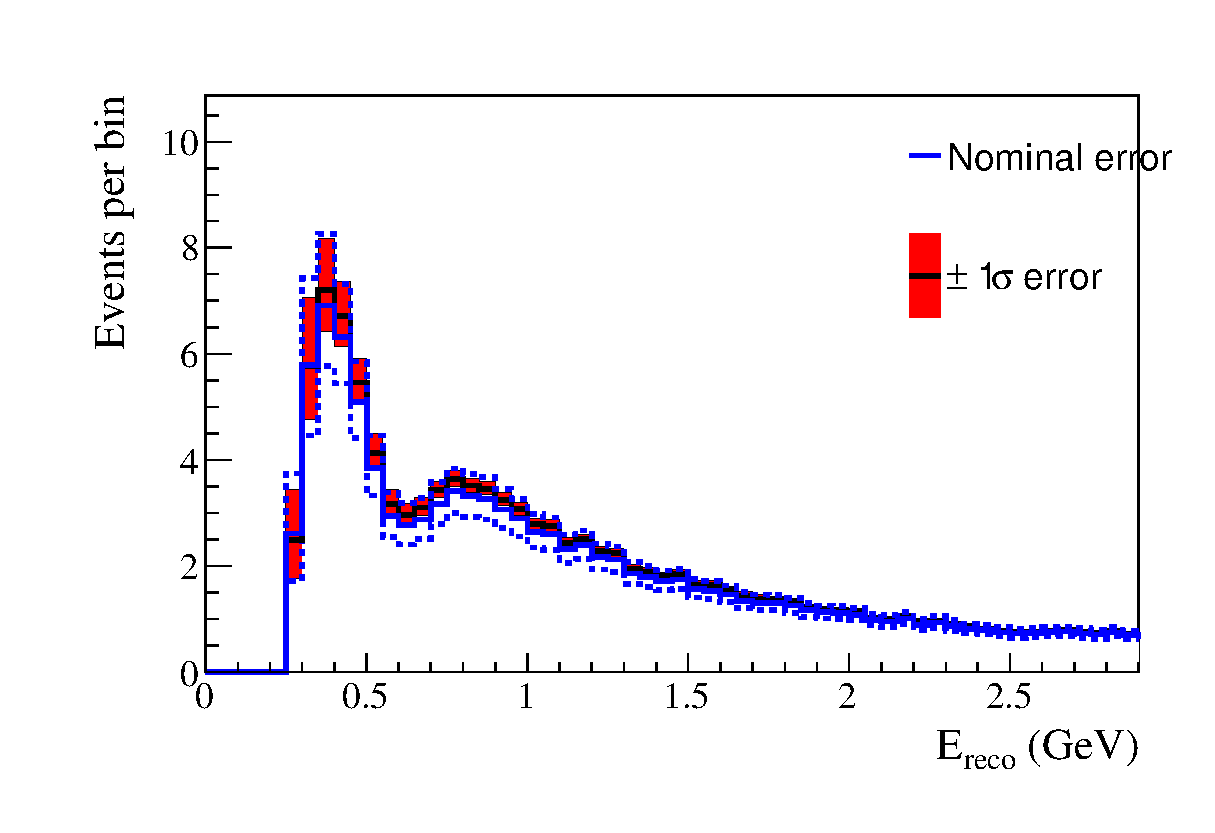
\includegraphics[width=0.9\textwidth]{joint_plots/systematics/Run17c/WithPreBANFF/Asimov_A_1Rmuoscillated_all_envelope.eps} 
\caption{Muon-like, neutrino mode}
\end{subfigure}
\begin{subfigure}[b]{0.49\textwidth} \centering
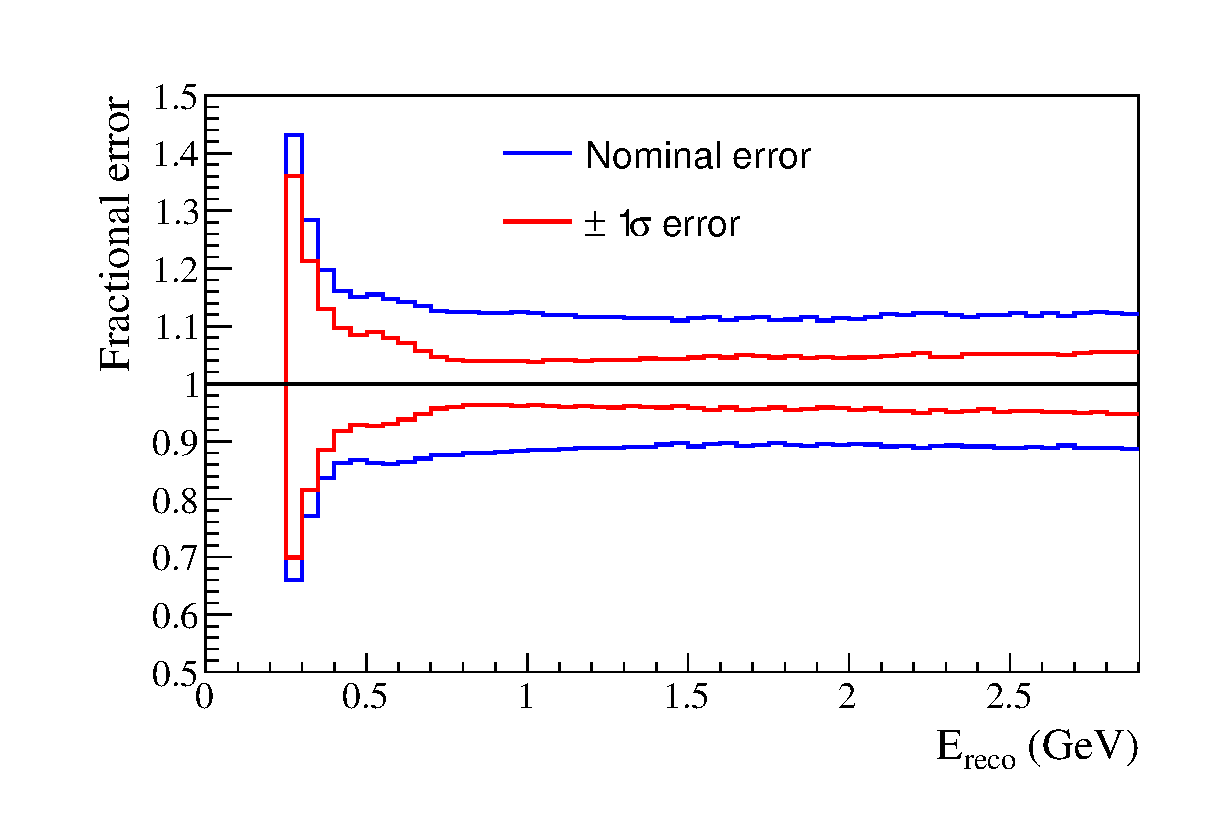
\includegraphics[width=0.9\textwidth]{joint_plots/systematics/Run17c/WithPreBANFF/Asimov_A_1Rmuoscillated_all_envelope_ratio.eps} \\
\caption{Muon-like, neutrino mode}
\end{subfigure}
%rhc mu-like
\begin{subfigure}[b]{0.49\textwidth} \centering
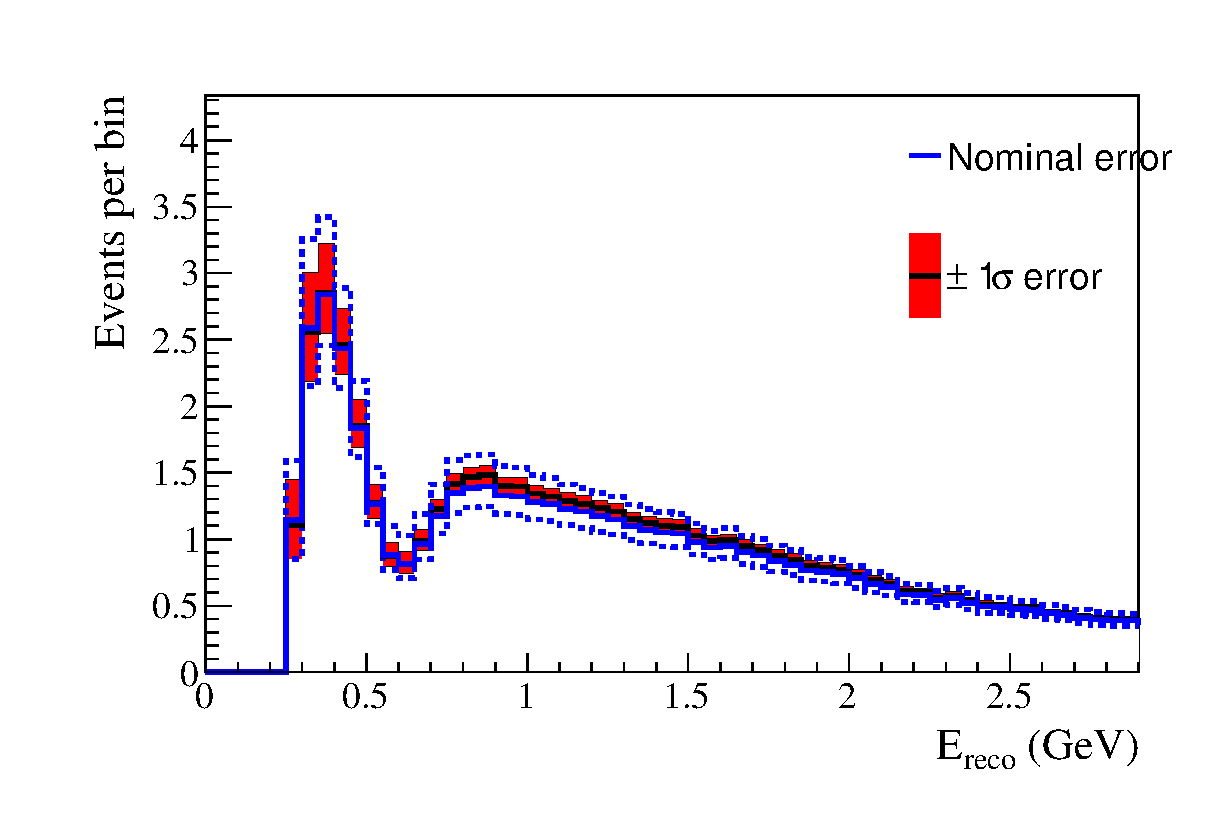
\includegraphics[width=0.9\textwidth]{joint_plots/systematics/Run17c/WithPreBANFF/Asimov_A_RHC1Rmuoscillated_all_envelope.eps} %\\ 
\caption{Muon-like, antineutrino mode}
\end{subfigure}
\begin{subfigure}[b]{0.49\textwidth} \centering
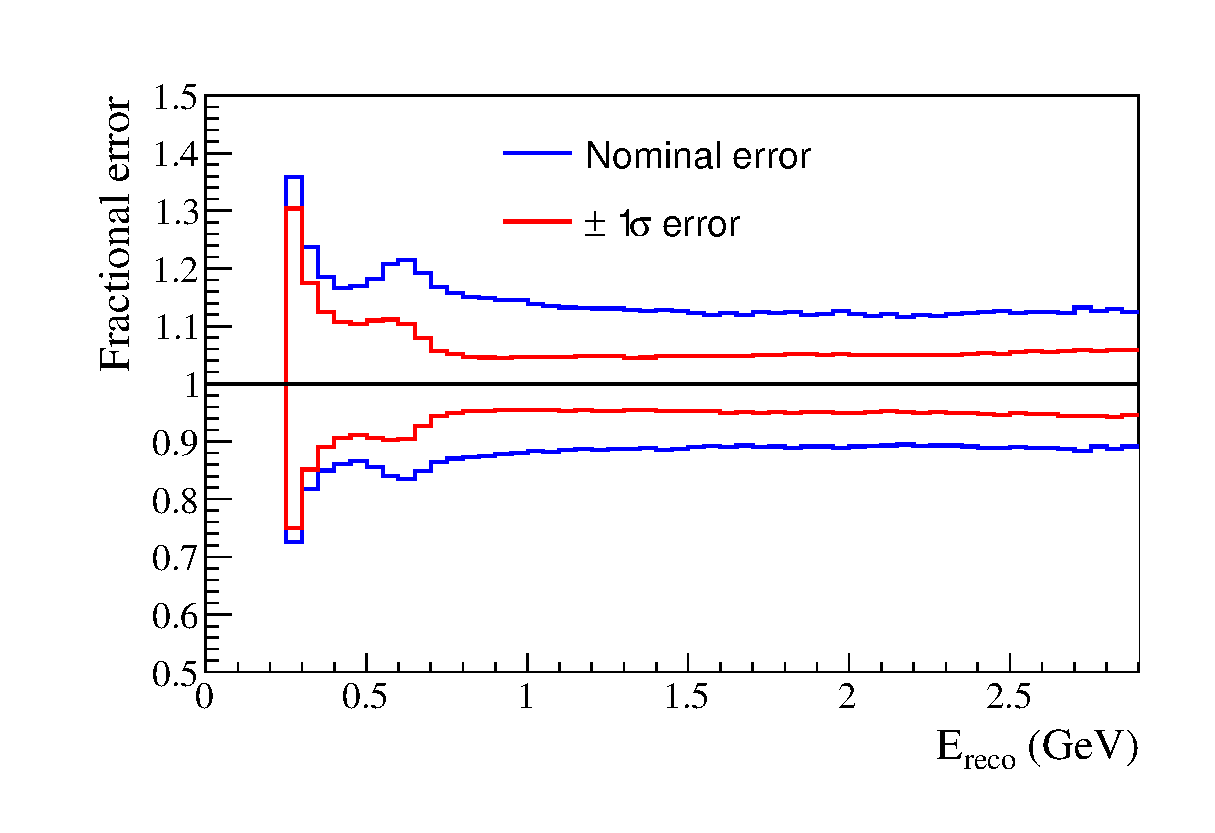
\includegraphics[width=0.9\textwidth]{joint_plots/systematics/Run17c/WithPreBANFF/Asimov_A_RHC1Rmuoscillated_all_envelope_ratio.eps} \\ 
\caption{Muon-like, antineutrino mode}
\end{subfigure}
%fhc e-like
\caption {
Error envelopes (left) and fractional errors (right) for the reconstructed neutrino energy spectrum
for all the systematic parameters.
Both pre- (blue), assuming the CCQE parameters to be gaussian distributed instead of flat, 
and post- (red) BANFF fit errors are shown.
	10k toy MC experiments are generated for the Asimov data set A shown in \cref{tab:osc_params_joint_asimov}
	with random systematic parameters, taking into account their correlations.
	Since the parameters $\delta_{CP}$, $\theta_{23}$ and $\Delta m^2_{32}$ ($\Delta m^2_{13}$) and mass hierarchy
will be measured,
only the uncertainty on 
$\sin^2 \theta_{13}$,
$\sin^2 \theta_{12}$
and 
$\Delta m^2_{21}$ 
are taken into account.
BANFF tuned MC templates are used. 
The distributions correspond to the collected statistics in the full Run 1-7c data set.
The changes due to the Run 1-7c flux and covariance matrix updates are applied.
}
\label{fig:spectra_systematic_Asimov_A_prebanff_run17c_mulike}
\end{figure*}


\begin{figure*}[htb]
\center

\begin{subfigure}[b]{0.49\textwidth} \centering
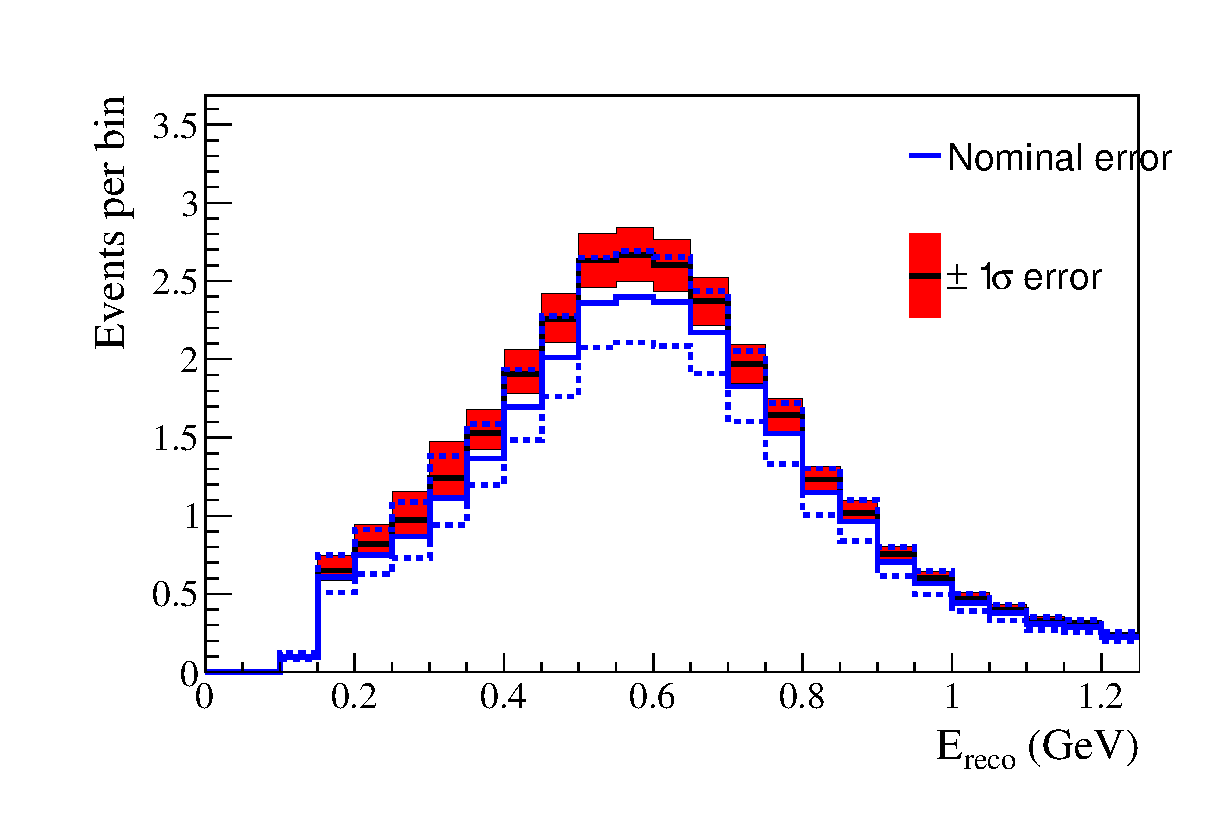
\includegraphics[width=0.9\textwidth]{joint_plots/systematics/Run17c/WithPreBANFF/Asimov_A_1Reoscillated_all_envelope.eps} 
\caption{Electron-like, neutrino mode}
\end{subfigure}
\begin{subfigure}[b]{0.49\textwidth} \centering
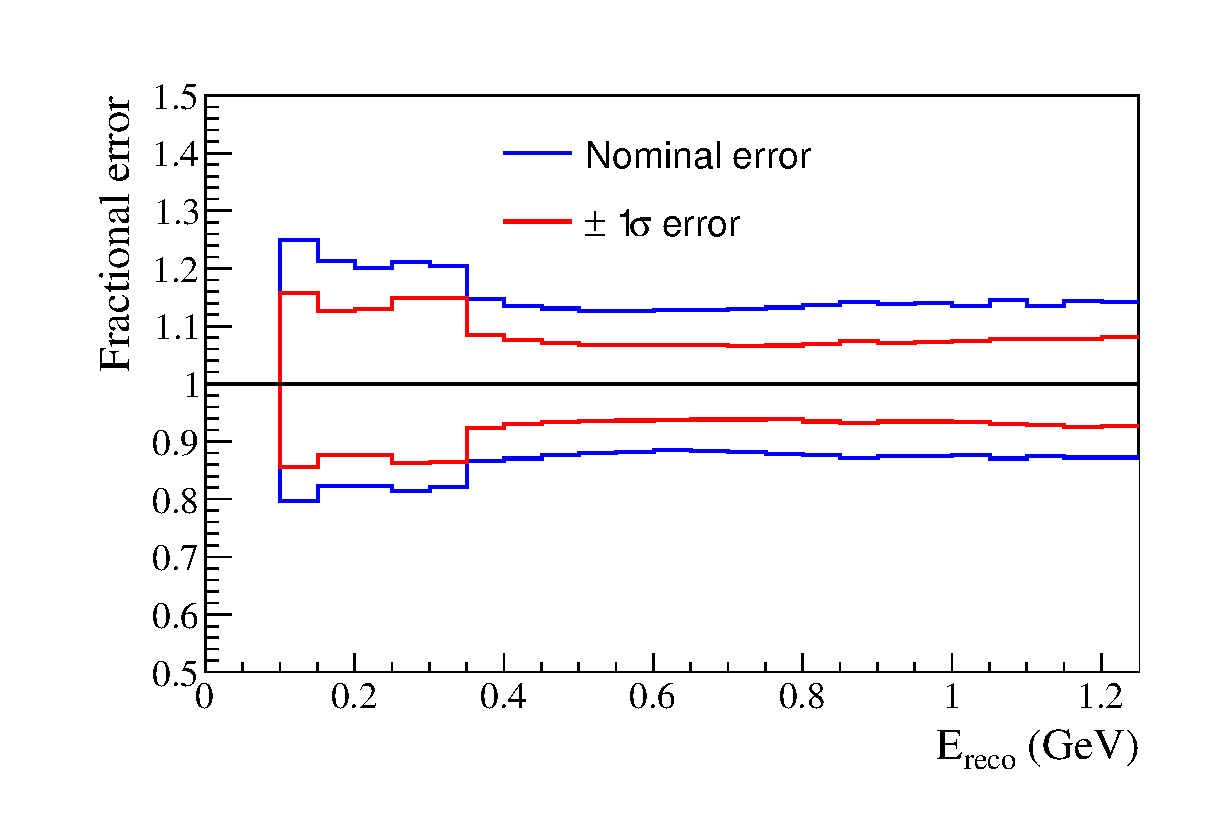
\includegraphics[width=0.9\textwidth]{joint_plots/systematics/Run17c/WithPreBANFF/Asimov_A_1Reoscillated_all_envelope_ratio.eps} 
\caption{Electron-like, neutrino mode}
\end{subfigure}
%rhc e-like
\begin{subfigure}[b]{0.49\textwidth} \centering
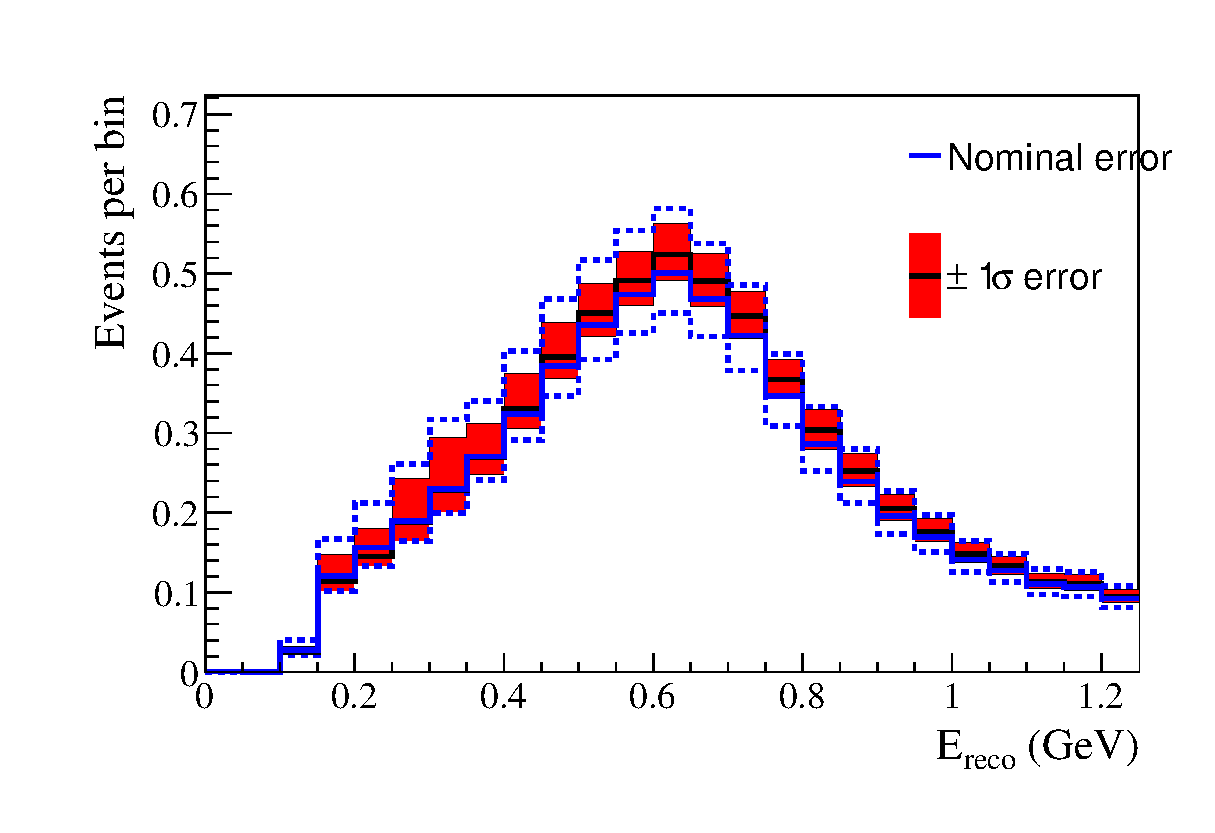
\includegraphics[width=0.9\textwidth]{joint_plots/systematics/Run17c/WithPreBANFF/Asimov_A_RHC1Reoscillated_all_envelope.eps} 
\caption{Electron-like, antineutrino mode}
\end{subfigure}
\begin{subfigure}[b]{0.49\textwidth} \centering
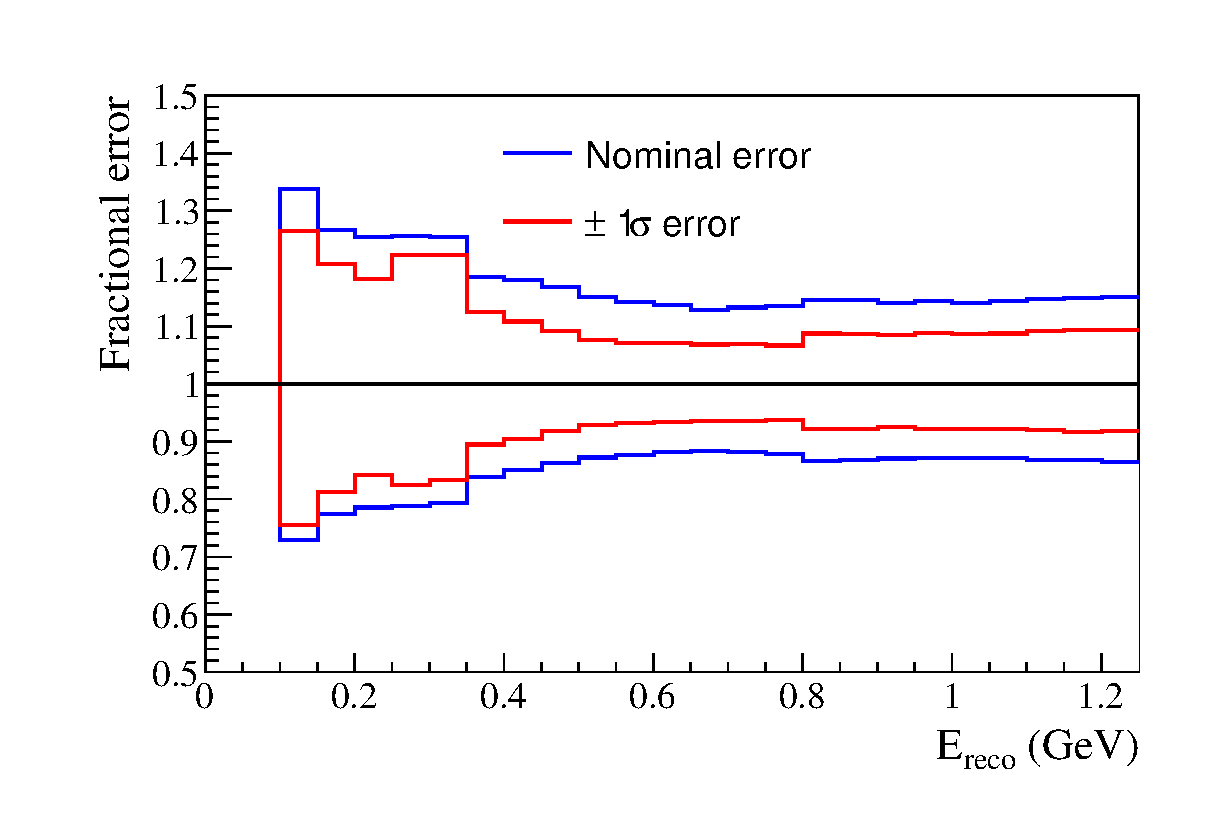
\includegraphics[width=0.9\textwidth]{joint_plots/systematics/Run17c/WithPreBANFF/Asimov_A_RHC1Reoscillated_all_envelope_ratio.eps} 
\caption{Electron-like, antineutrino mode}
\end{subfigure}
%fhc ccpi-like
\begin{subfigure}[b]{0.49\textwidth} \centering
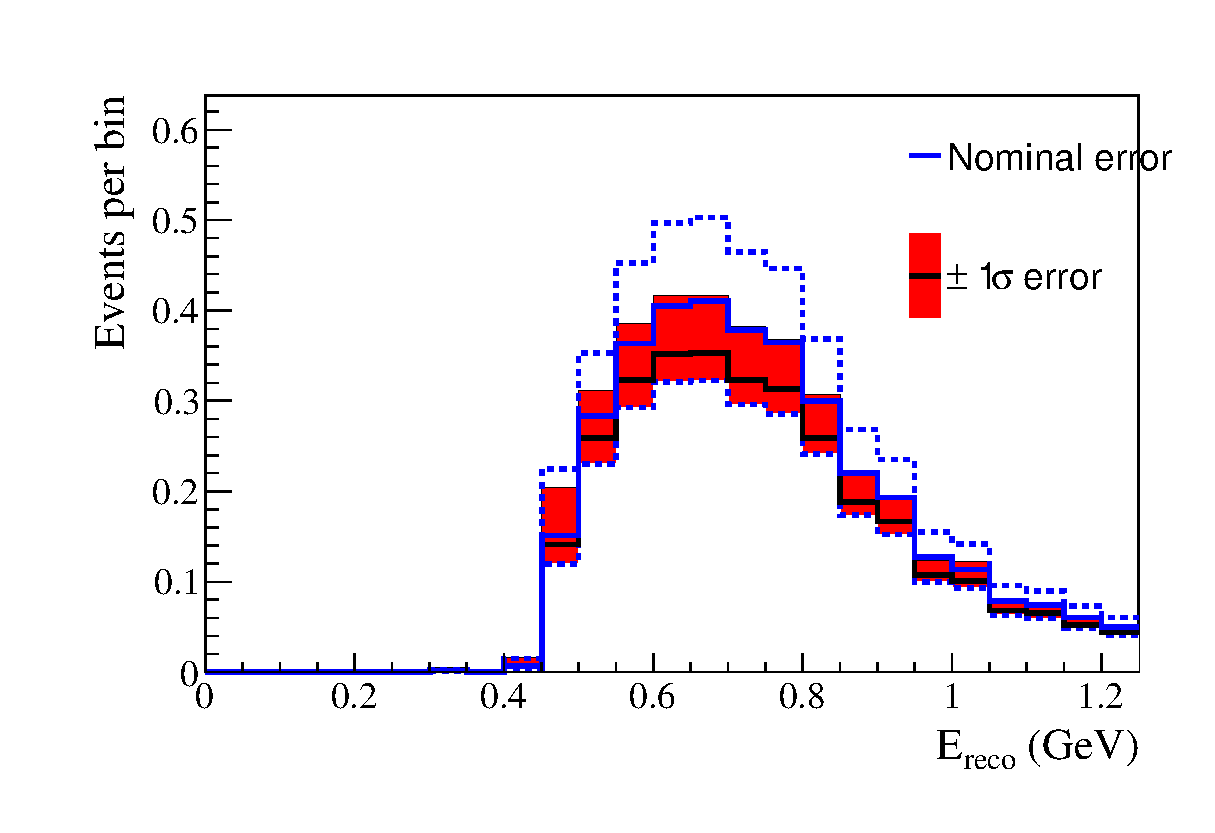
\includegraphics[width=0.9\textwidth]{joint_plots/systematics/Run17c/WithPreBANFF/Asimov_A_MultiReoscillated_all_envelope.eps} 
\caption{\nueCConepi{}, neutrino mode}
\end{subfigure}
\begin{subfigure}[b]{0.49\textwidth} \centering
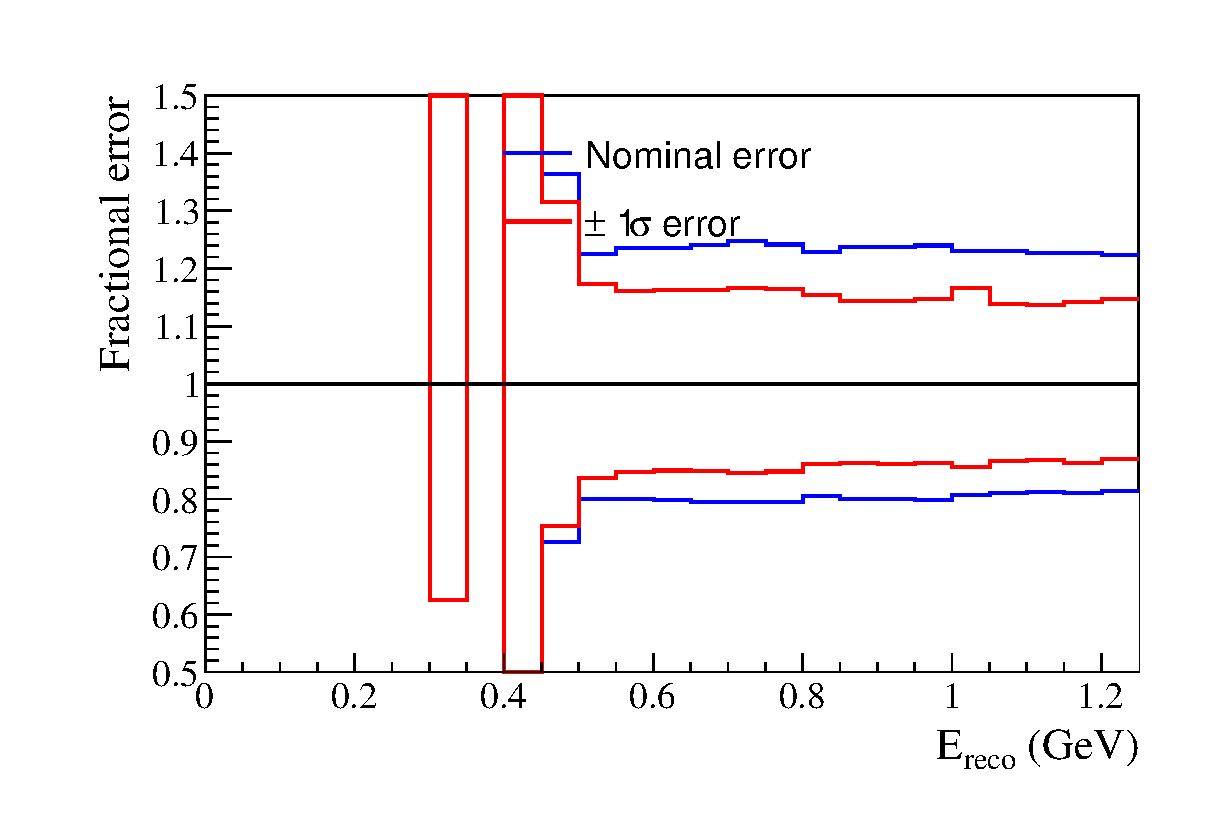
\includegraphics[width=0.9\textwidth]{joint_plots/systematics/Run17c/WithPreBANFF/Asimov_A_MultiReoscillated_all_envelope_ratio.eps} 
\caption{\nueCConepi{}, neutrino mode}
\end{subfigure}
\caption {
Error envelopes (left) and fractional errors (right) for the reconstructed neutrino energy spectrum
for all the systematic parameters.
Both pre- (blue), assuming the CCQE parameters to be gaussian distributed instead of flat, 
and post- (red) BANFF fit errors are shown.
10k toy MC experiments are generated for the Asimov data set A shown in \cref{tab:osc_params_joint_asimov}
with randomised systematic parameters, taking into account their correlations.
Since the parameters $\delta_{CP}$, $\theta_{23}$ and $\Delta m^2_{32}$ ($\Delta m^2_{13}$) and mass hierarchy
will be measured,
only the uncertainty on 
$\sin^2 \theta_{13}$,
$\sin^2 \theta_{12}$
and 
$\Delta m^2_{21}$ 
are taken into account.
BANFF tuned MC templates are used. 
The distributions correspond to the collected statistics in the full Run 1-7c data set.
The changes due to the Run 1-7c flux and covariance matrix updates are applied.
}
\label{fig:spectra_systematic_Asimov_A_prebanff_run17c_elike}
\end{figure*}




\begin{figure*}[htb]
\center
%fhc mu-like
\begin{subfigure}[b]{0.49\textwidth} \centering
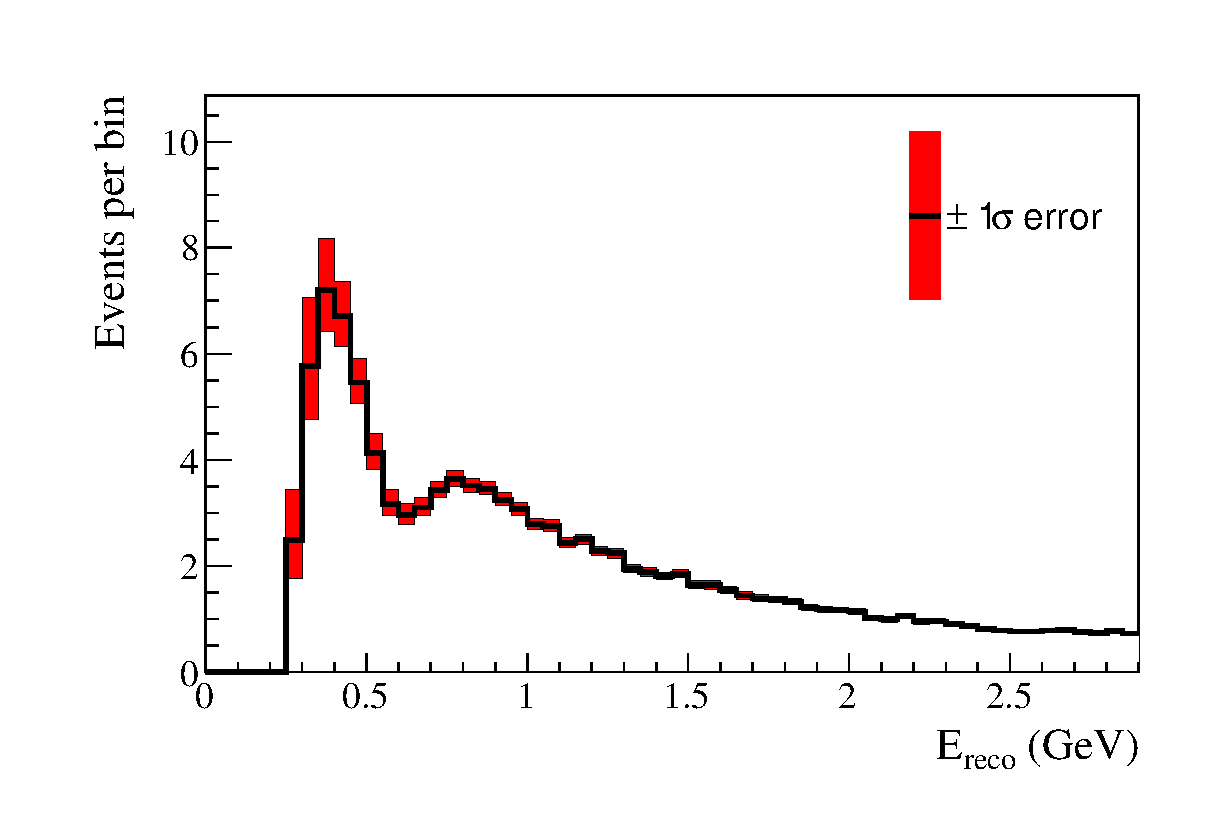
\includegraphics[width=0.9\textwidth]{joint_plots/systematics/Run17c/Asimov_A_1Rmuoscillated_all_envelope.eps} 
\caption{Muon-like, neutrino mode}
\end{subfigure}
\begin{subfigure}[b]{0.49\textwidth} \centering
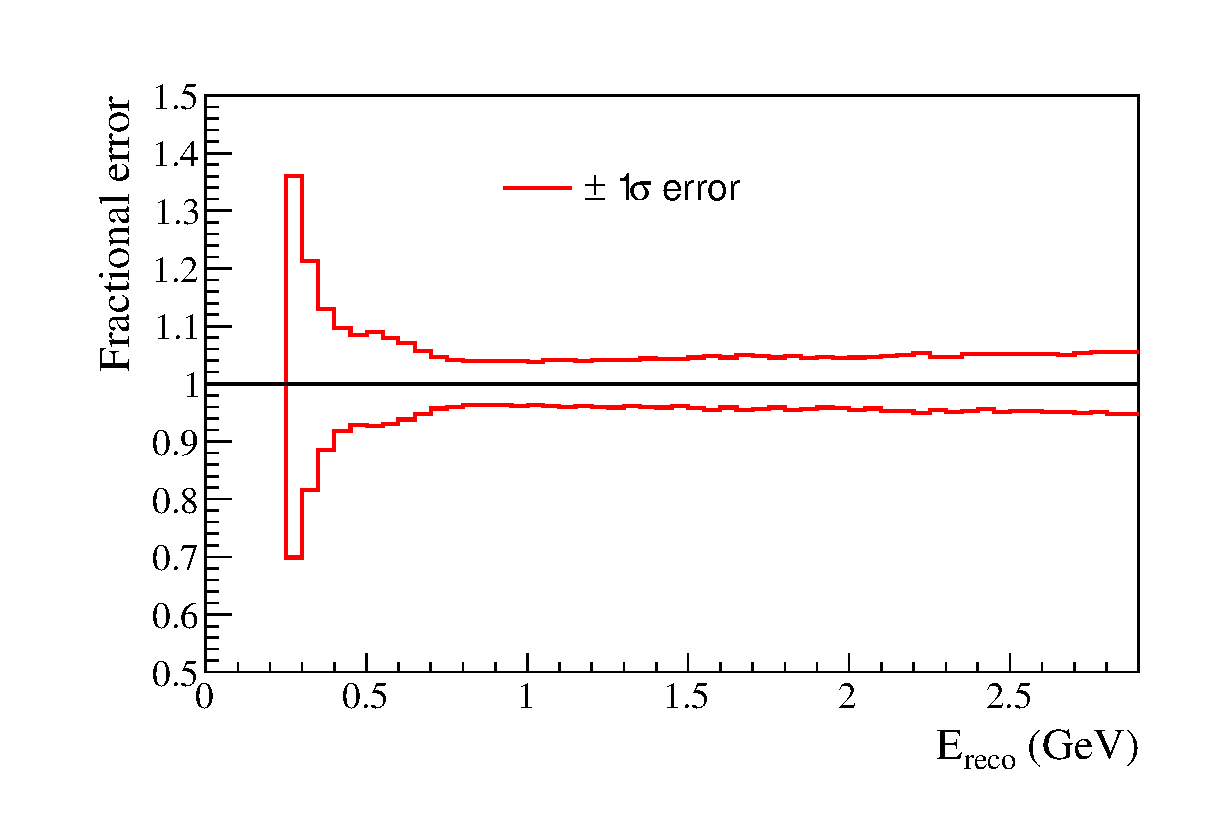
\includegraphics[width=0.9\textwidth]{joint_plots/systematics/Run17c/Asimov_A_1Rmuoscillated_all_envelope_ratio.eps} \\
\caption{Muon-like, neutrino mode}
\end{subfigure}
%rhc mu-like
\begin{subfigure}[b]{0.49\textwidth} \centering
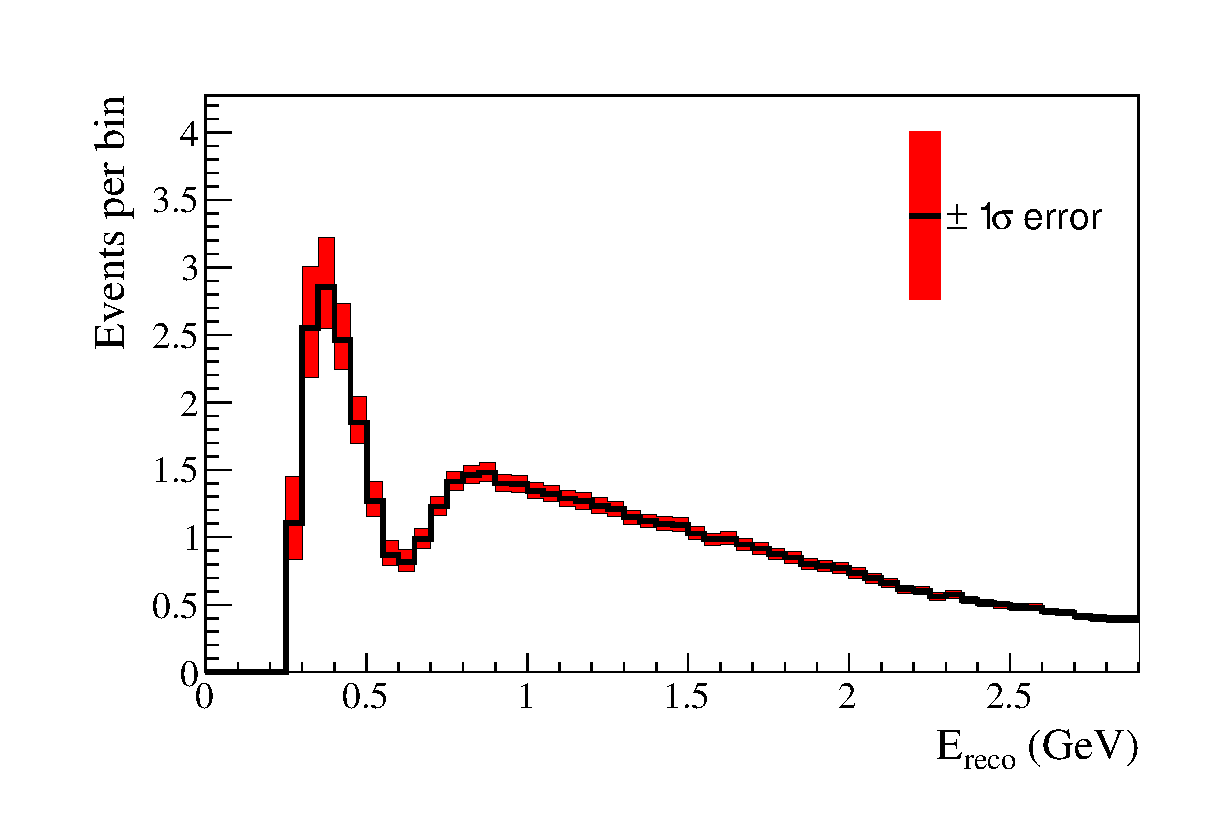
\includegraphics[width=0.9\textwidth]{joint_plots/systematics/Run17c/Asimov_A_RHC1Rmuoscillated_all_envelope.eps} %\\ 
\caption{Muon-like, antineutrino mode}
\end{subfigure}
\begin{subfigure}[b]{0.49\textwidth} \centering
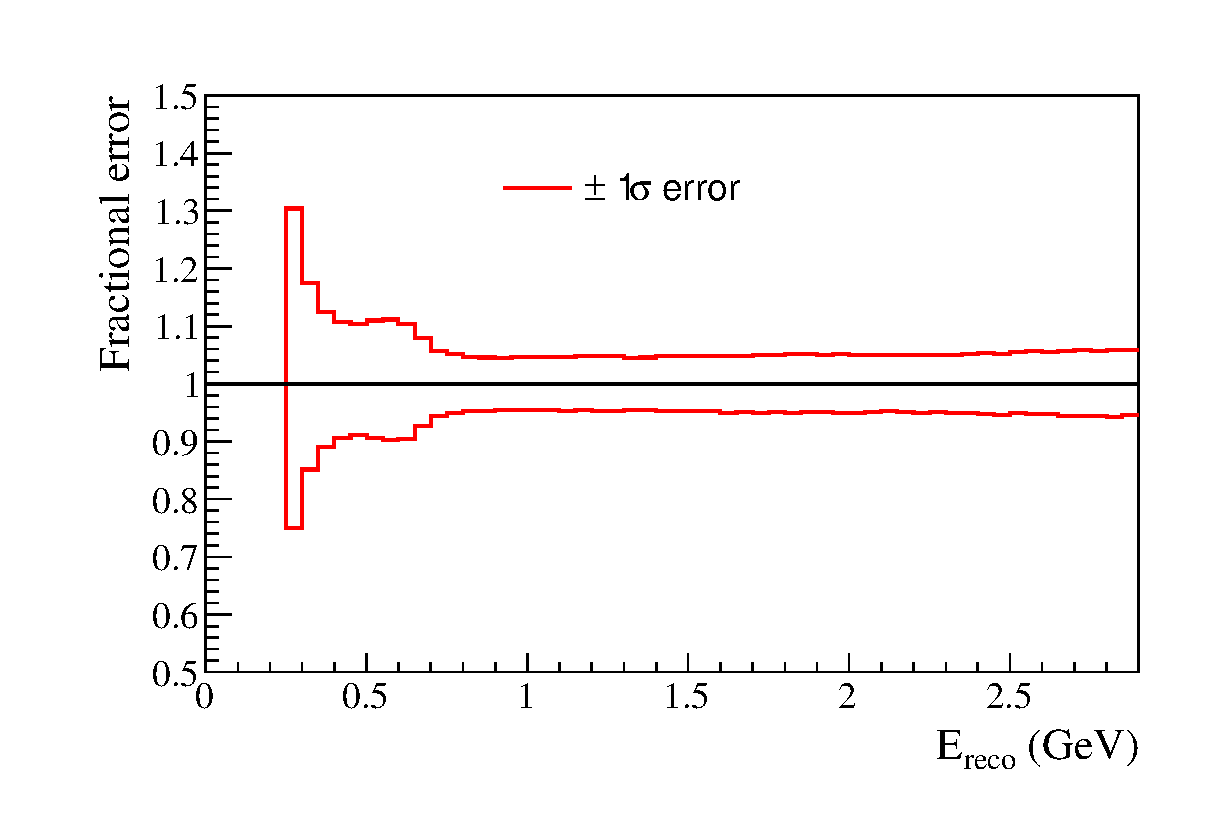
\includegraphics[width=0.9\textwidth]{joint_plots/systematics/Run17c/Asimov_A_RHC1Rmuoscillated_all_envelope_ratio.eps} \\ 
\caption{Muon-like, antineutrino mode}
\end{subfigure}
%fhc e-like
\caption {
Error envelopes (left) and fractional errors (right) for the reconstructed neutrino energy spectrum
for all the systematic parameters.
	10k toy MC experiments are generated for the Asimov data set A shown in \cref{tab:osc_params_joint_asimov}
	with random systematic parameters, taking into account their correlations.
	Since the parameters $\delta_{CP}$, $\theta_{23}$ and $\Delta m^2_{32}$ ($\Delta m^2_{13}$) and mass hierarchy
will be measured,
only the uncertainty on 
$\sin^2 \theta_{13}$,
$\sin^2 \theta_{12}$
and 
$\Delta m^2_{21}$ 
are taken into account.
BANFF tuned MC templates are used. 
The distributions correspond to the collected statistics in the full Run 1-7c data set.
The changes due to the Run 1-7c flux and covariance matrix updates are applied.
}
\label{fig:spectra_systematic_Asimov_A_run17c_mulike}
\end{figure*}


\begin{figure*}[htb]
\center

\begin{subfigure}[b]{0.49\textwidth} \centering
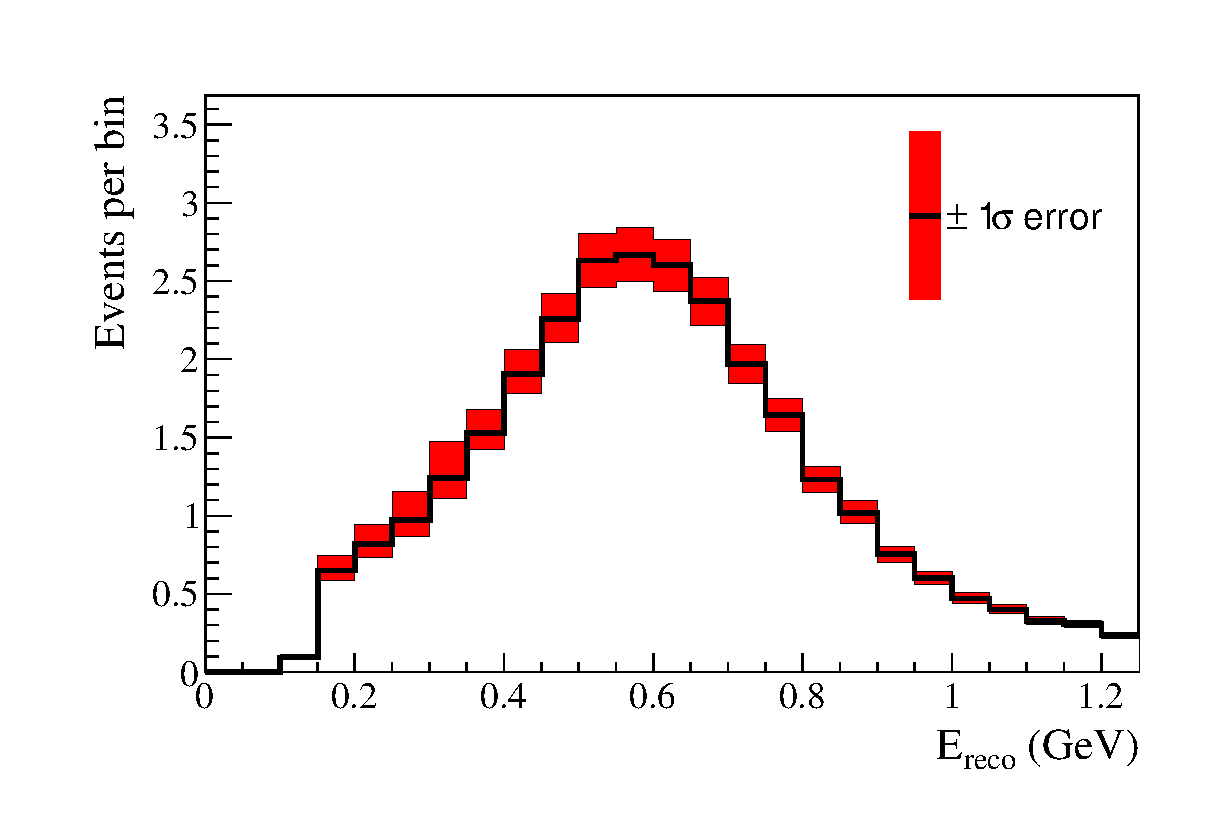
\includegraphics[width=0.9\textwidth]{joint_plots/systematics/Run17c/Asimov_A_1Reoscillated_all_envelope.eps} 
\caption{Electron-like, neutrino mode}
\end{subfigure}
\begin{subfigure}[b]{0.49\textwidth} \centering
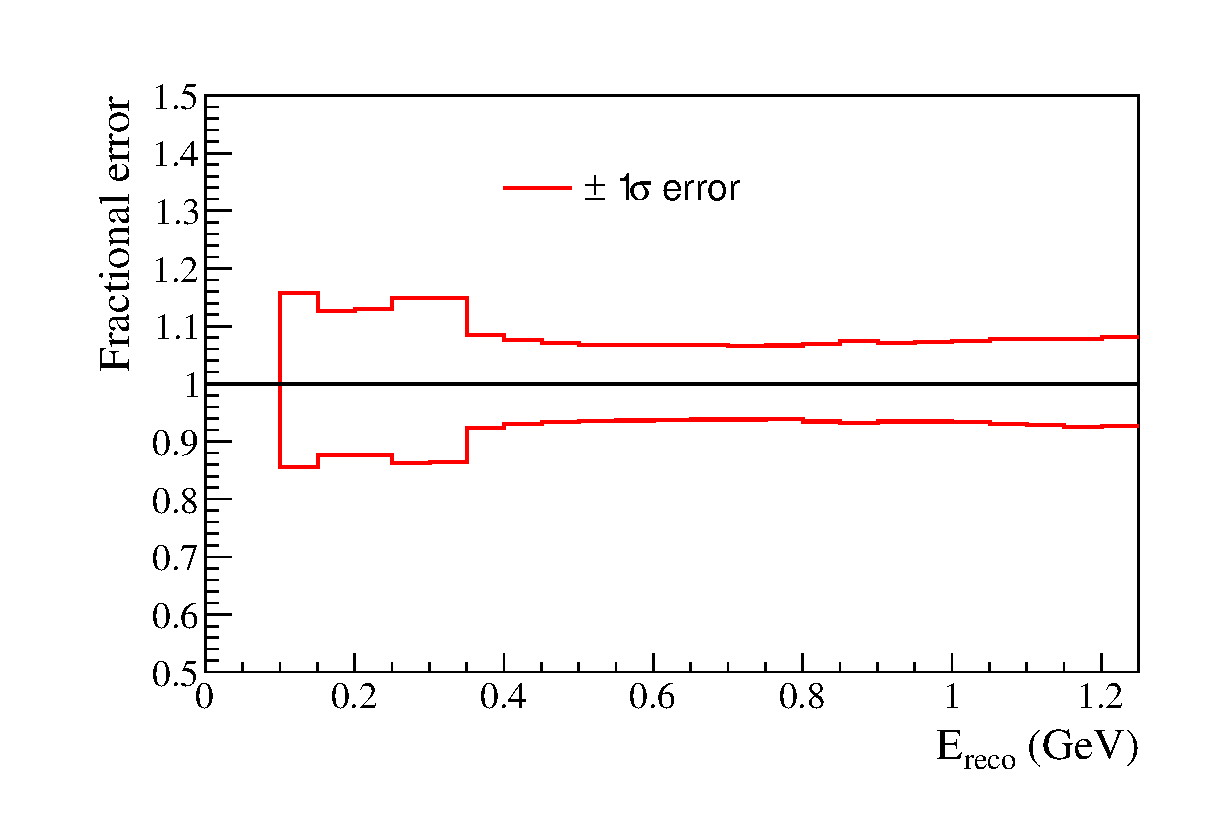
\includegraphics[width=0.9\textwidth]{joint_plots/systematics/Run17c/Asimov_A_1Reoscillated_all_envelope_ratio.eps} 
\caption{Electron-like, neutrino mode}
\end{subfigure}
%rhc e-like
\begin{subfigure}[b]{0.49\textwidth} \centering
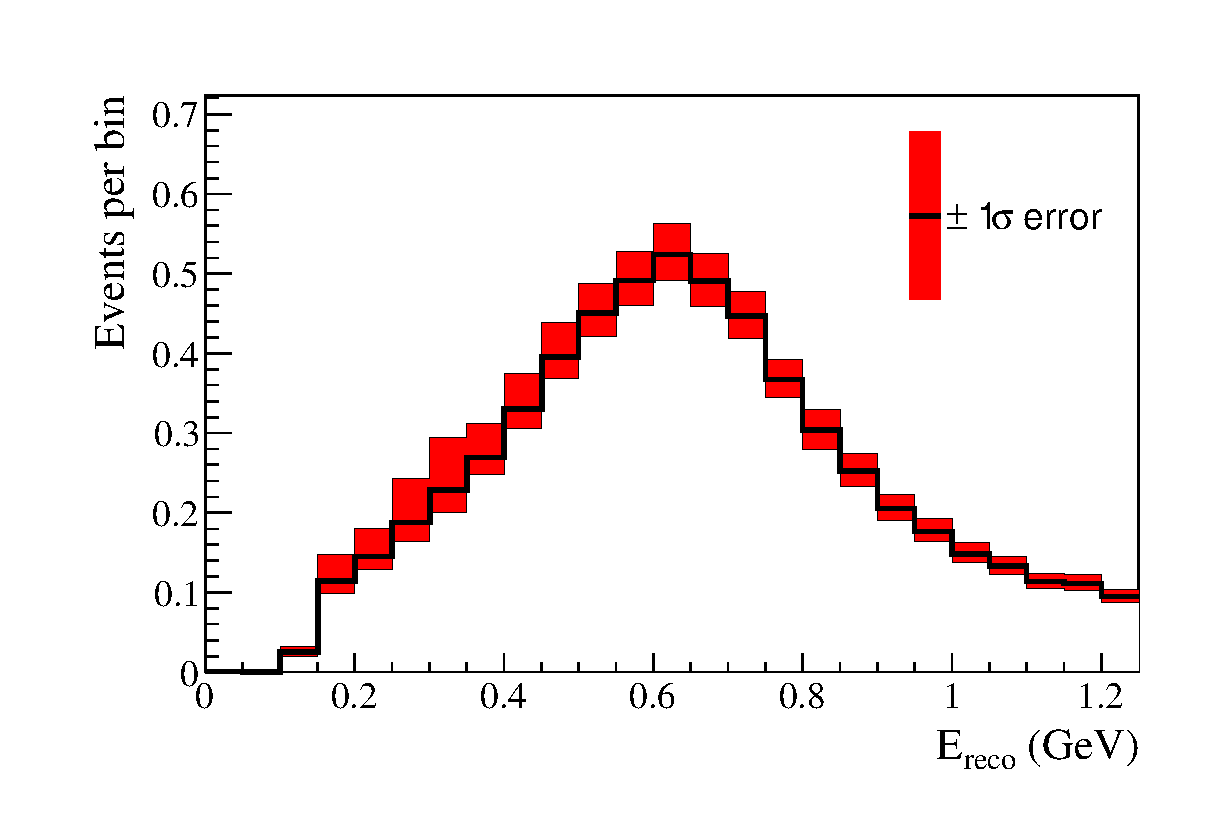
\includegraphics[width=0.9\textwidth]{joint_plots/systematics/Run17c/Asimov_A_RHC1Reoscillated_all_envelope.eps} 
\caption{Electron-like, antineutrino mode}
\end{subfigure}
\begin{subfigure}[b]{0.49\textwidth} \centering
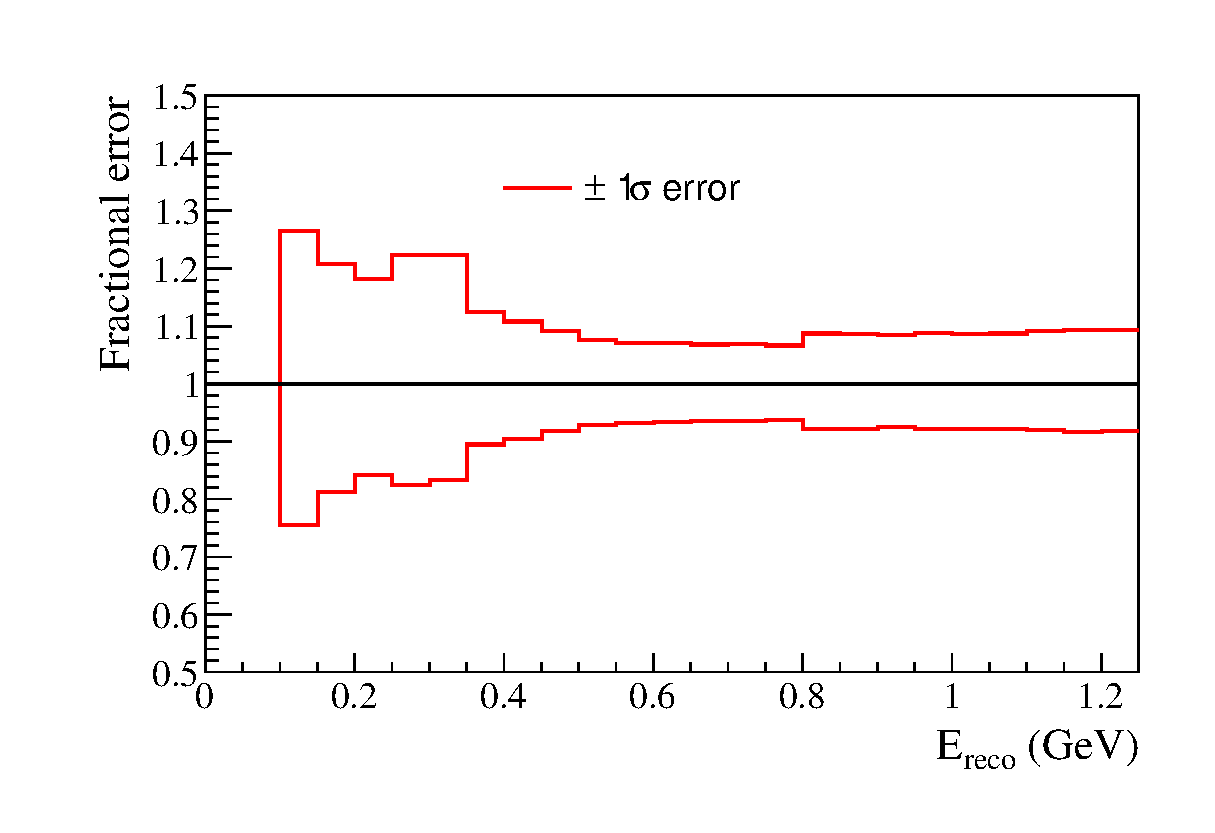
\includegraphics[width=0.9\textwidth]{joint_plots/systematics/Run17c/Asimov_A_RHC1Reoscillated_all_envelope_ratio.eps} 
\caption{Electron-like, antineutrino mode}
\end{subfigure}
%fhc e-like
\begin{subfigure}[b]{0.49\textwidth} \centering
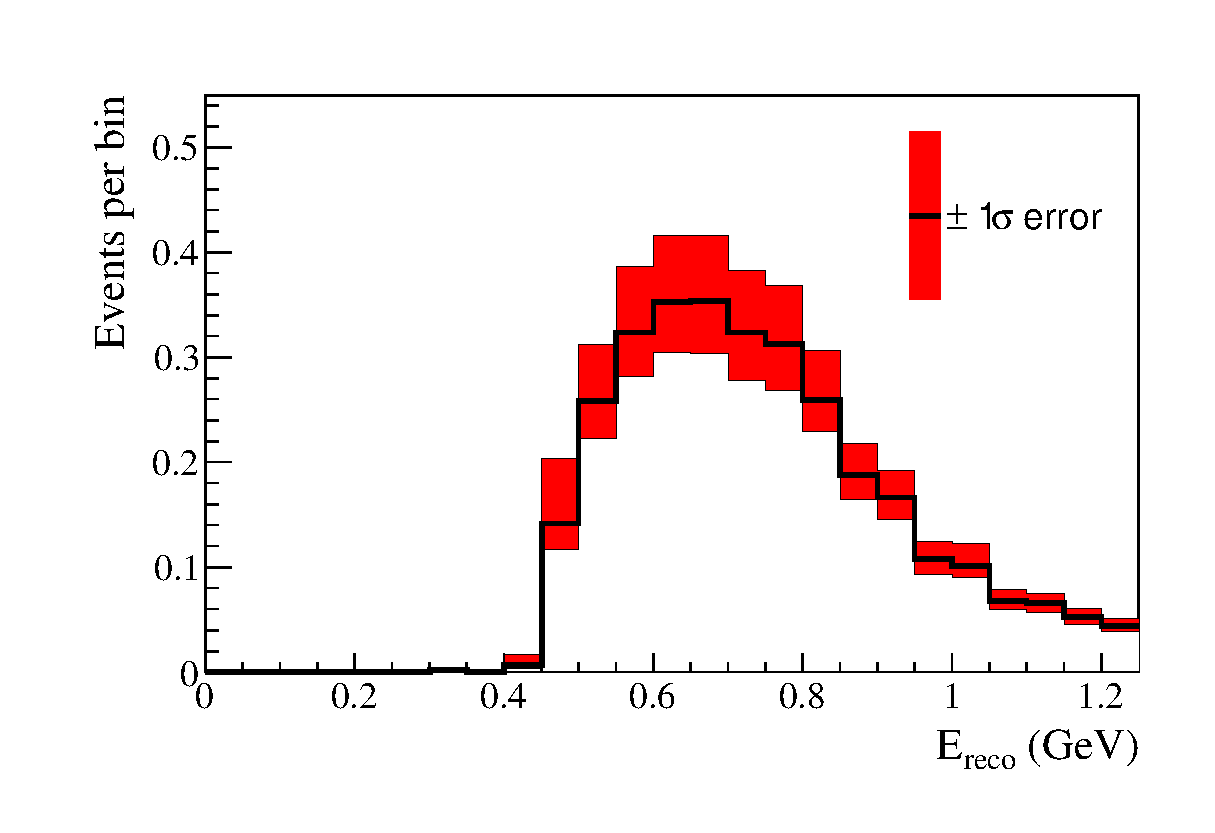
\includegraphics[width=0.9\textwidth]{joint_plots/systematics/Run17c/Asimov_A_MultiReoscillated_all_envelope.eps} 
\caption{\nueCConepi{}, neutrino mode}
\end{subfigure}
\begin{subfigure}[b]{0.49\textwidth} \centering
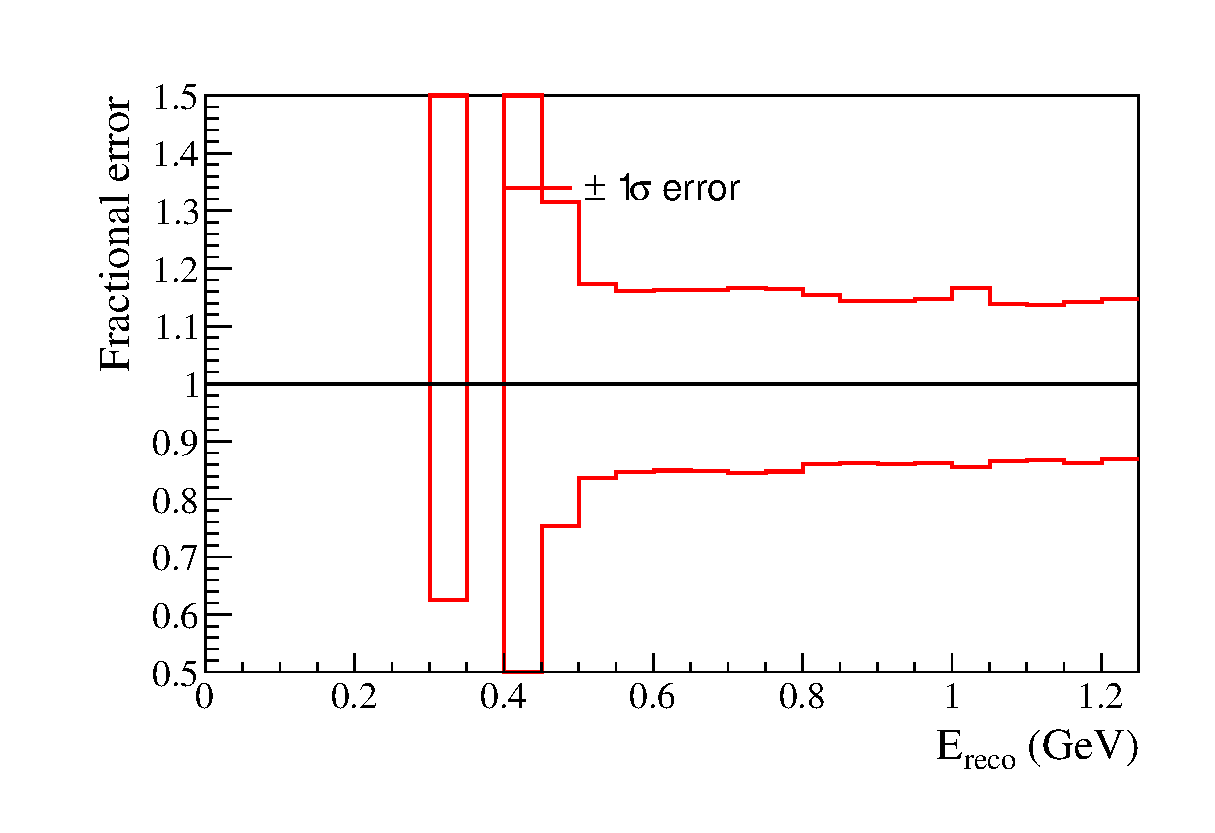
\includegraphics[width=0.9\textwidth]{joint_plots/systematics/Run17c/Asimov_A_MultiReoscillated_all_envelope_ratio.eps} 
\caption{\nueCConepi{}, neutrino mode}
\end{subfigure}
\caption {
Error envelopes (left) and fractional errors (right) for the reconstructed neutrino energy spectrum
for all the systematic parameters.
10k toy MC experiments are generated for the Asimov data set A shown in \cref{tab:osc_params_joint_asimov}
with randomised systematic parameters, taking into account their correlations.
Since the parameters $\delta_{CP}$, $\theta_{23}$ and $\Delta m^2_{32}$ ($\Delta m^2_{13}$) and mass hierarchy
will be measured,
only the uncertainty on 
$\sin^2 \theta_{13}$,
$\sin^2 \theta_{12}$
and 
$\Delta m^2_{21}$ 
are taken into account.
BANFF tuned MC templates are used. 
The distributions correspond to the collected statistics in the full Run 1-7c data set.
The changes due to the Run 1-7c flux and covariance matrix updates are applied.
}
\label{fig:spectra_systematic_Asimov_A_run17c_elike}
\end{figure*}



%%%% Single systematic sources of Asimov A


\begin{figure*}[htb]
\center
%fhc mu-like
\begin{subfigure}[b]{0.49\textwidth} \centering
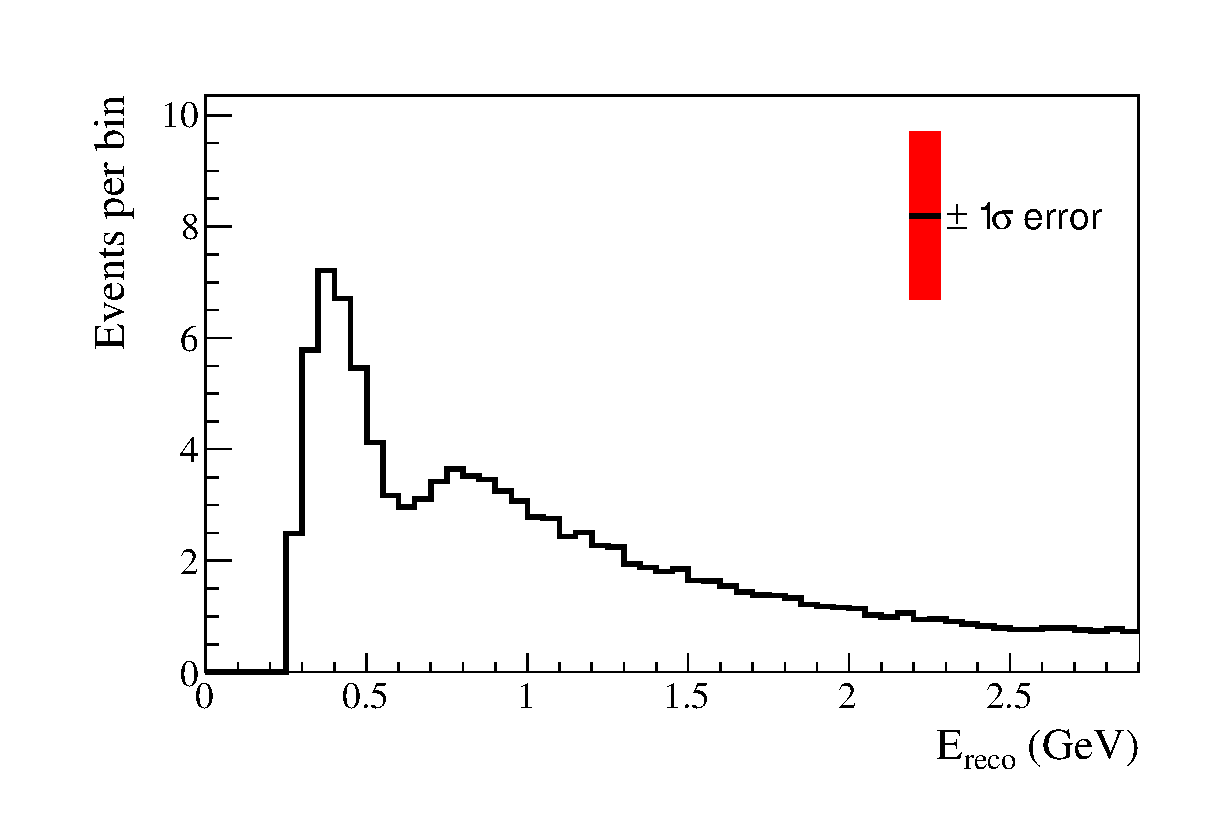
\includegraphics[width=0.9\textwidth]{joint_plots/systematics/Run17c/Asimov_A_1Rmuoscillated_Osc_param_envelope.eps}
\caption{Muon-like, neutrino mode}
\end{subfigure}
\begin{subfigure}[b]{0.49\textwidth} \centering
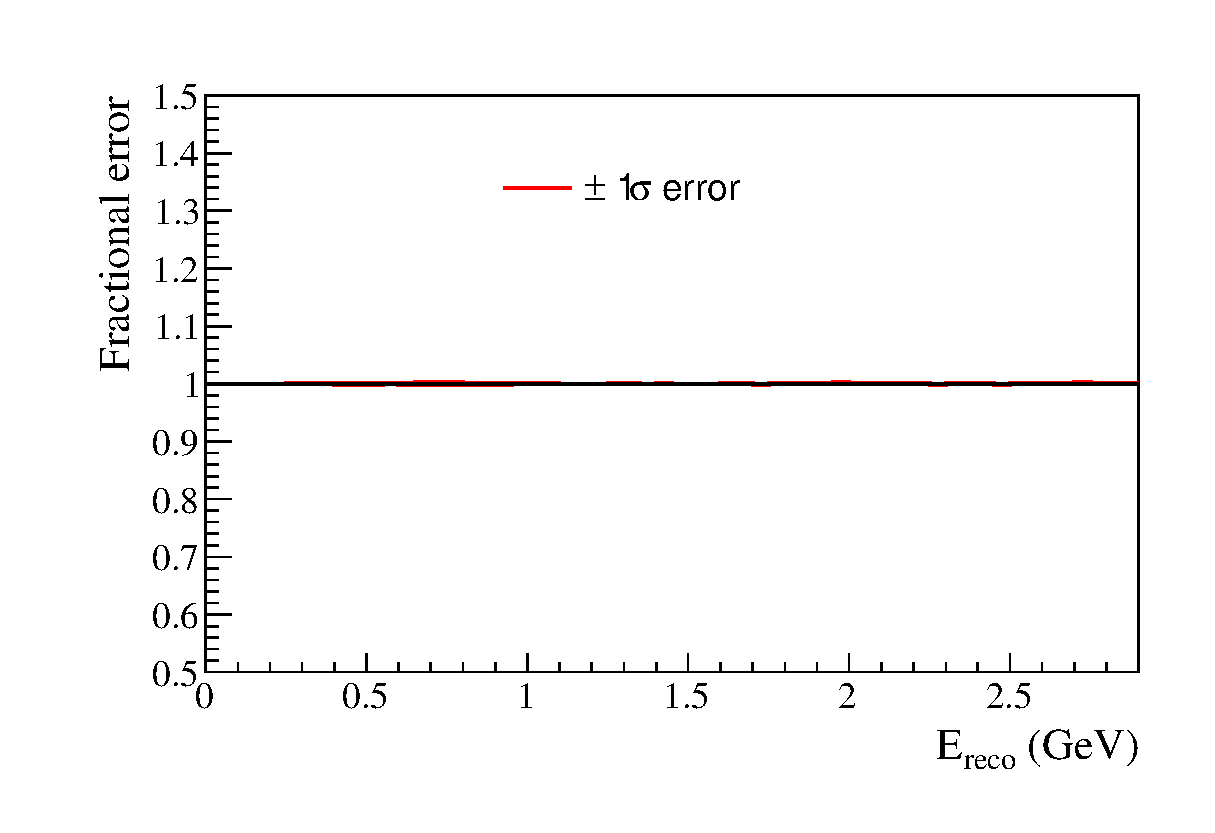
\includegraphics[width=0.9\textwidth]{joint_plots/systematics/Run17c/Asimov_A_1Rmuoscillated_Osc_param_envelope_ratio.eps} 
\caption{Muon-like, neutrino mode}
\end{subfigure}
%rhc mu-like
\begin{subfigure}[b]{0.49\textwidth} \centering
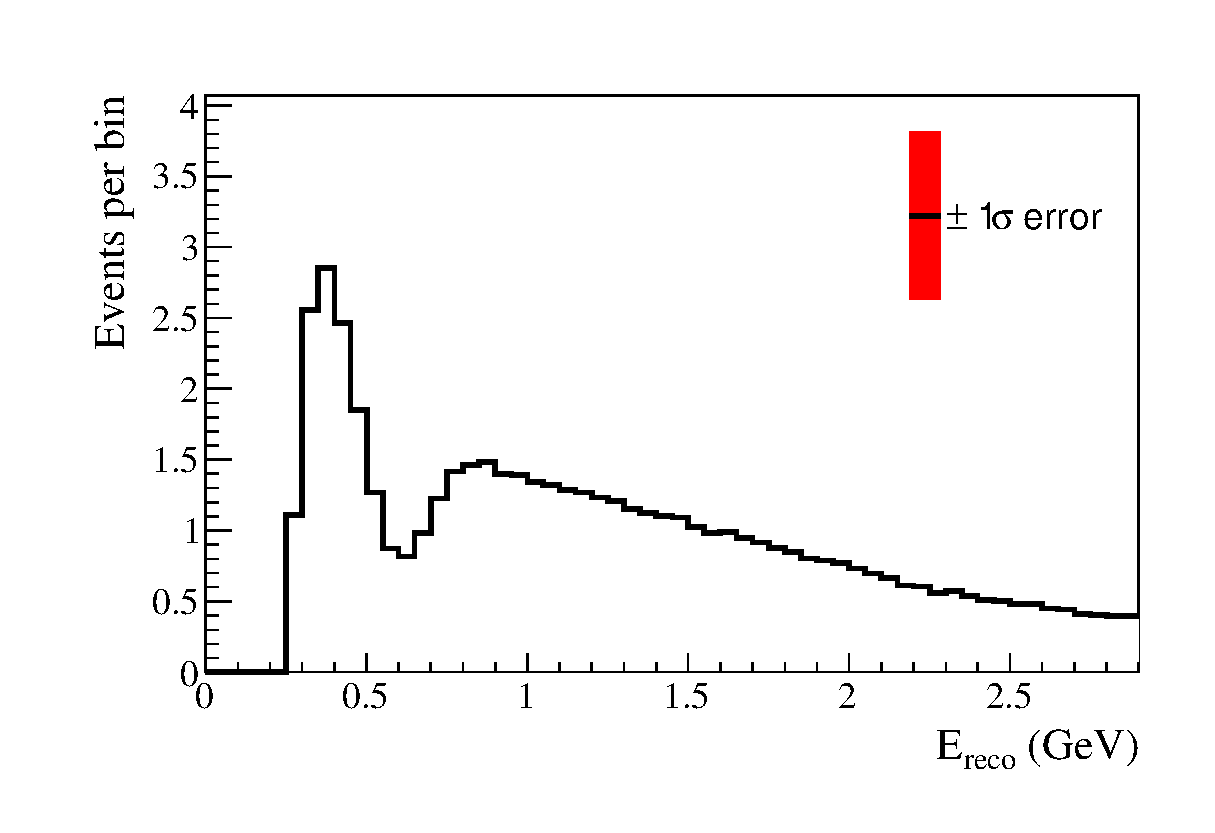
\includegraphics[width=0.9\textwidth]{joint_plots/systematics/Run17c/Asimov_A_RHC1Rmuoscillated_Osc_param_envelope.eps} \\ 
\caption{Muon-like, antineutrino mode}
\end{subfigure}
\begin{subfigure}[b]{0.49\textwidth} \centering
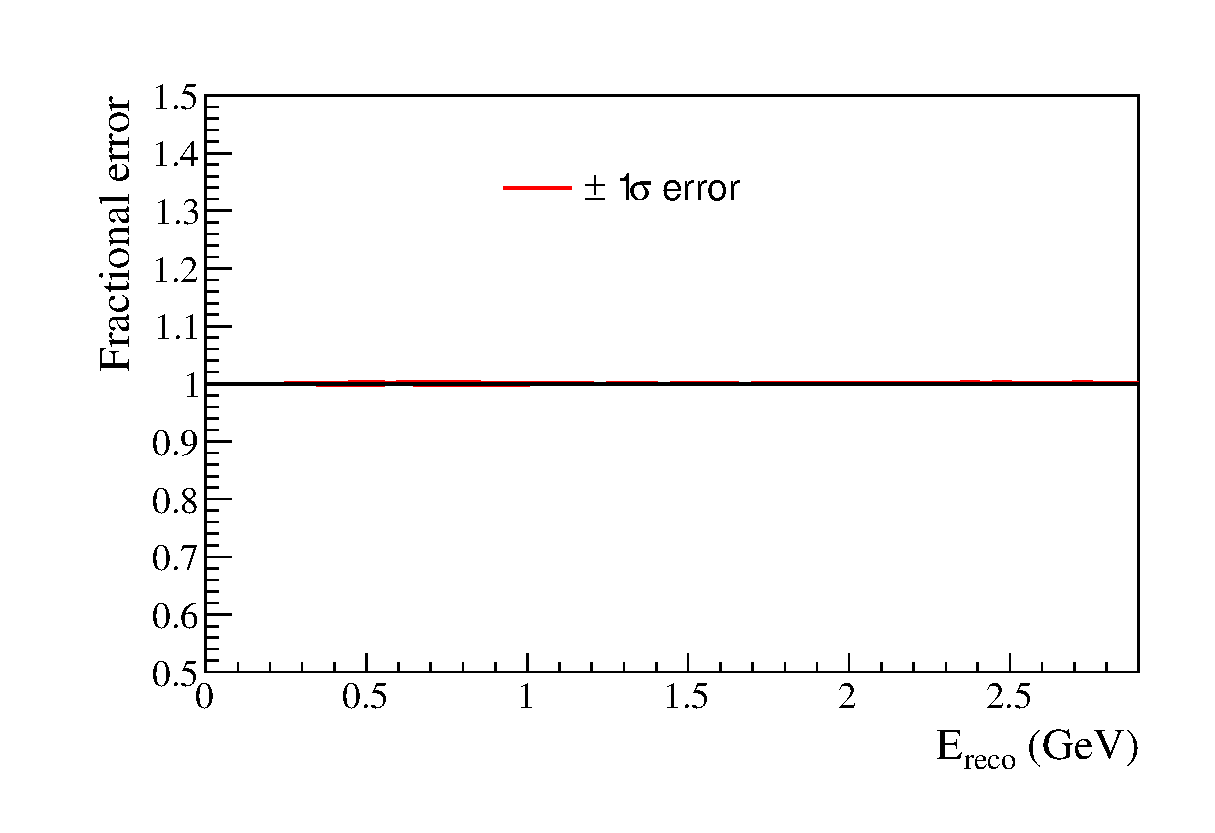
\includegraphics[width=0.9\textwidth]{joint_plots/systematics/Run17c/Asimov_A_RHC1Rmuoscillated_Osc_param_envelope_ratio.eps} \\ 
\caption{Muon-like, antineutrino mode}
\end{subfigure}
%fhc e-like
\caption {
Error envelopes (left) and fractional errors (right) for the reconstructed neutrino energy spectrum
as a result of the oscillation systematic parameters.
	10k toy MC experiments are generated for the Asimov data set A shown in \cref{tab:osc_params_joint_asimov}
	with random systematic parameters, taking into account their correlations.
	Since the parameters $\delta_{CP}$, $\theta_{23}$ and $\Delta m^2_{32}$ ($\Delta m^2_{13}$) and mass hierarchy
will be measured,
only the uncertainty on 
$\sin^2 \theta_{13}$,
$\sin^2 \theta_{12}$
and 
$\Delta m^2_{21}$ 
are taken into account.
BANFF tuned MC templates are used. 
The distributions correspond to the collected statistics in the full Run 1-7c data set.
The changes due to the Run 1-7c flux and covariance matrix updates are applied.
}
\label{fig:Osc_envelope_Asimov_A_run17c_mulike}
\end{figure*}


\begin{figure*}[htb]
\center

\begin{subfigure}[b]{0.49\textwidth} \centering
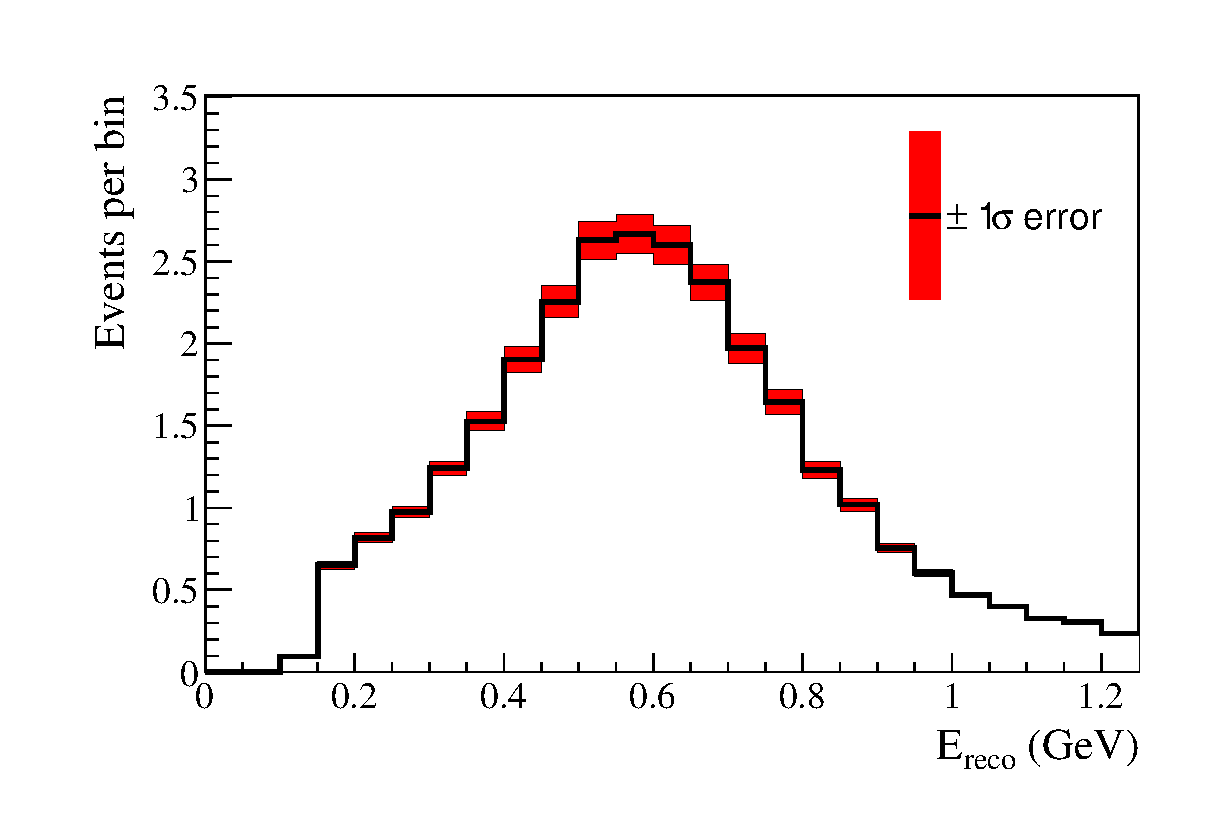
\includegraphics[width=0.9\textwidth]{joint_plots/systematics/Run17c/Asimov_A_1Reoscillated_Osc_param_envelope.eps} 
\caption{Electron-like, neutrino mode}
\end{subfigure}
\begin{subfigure}[b]{0.49\textwidth} \centering
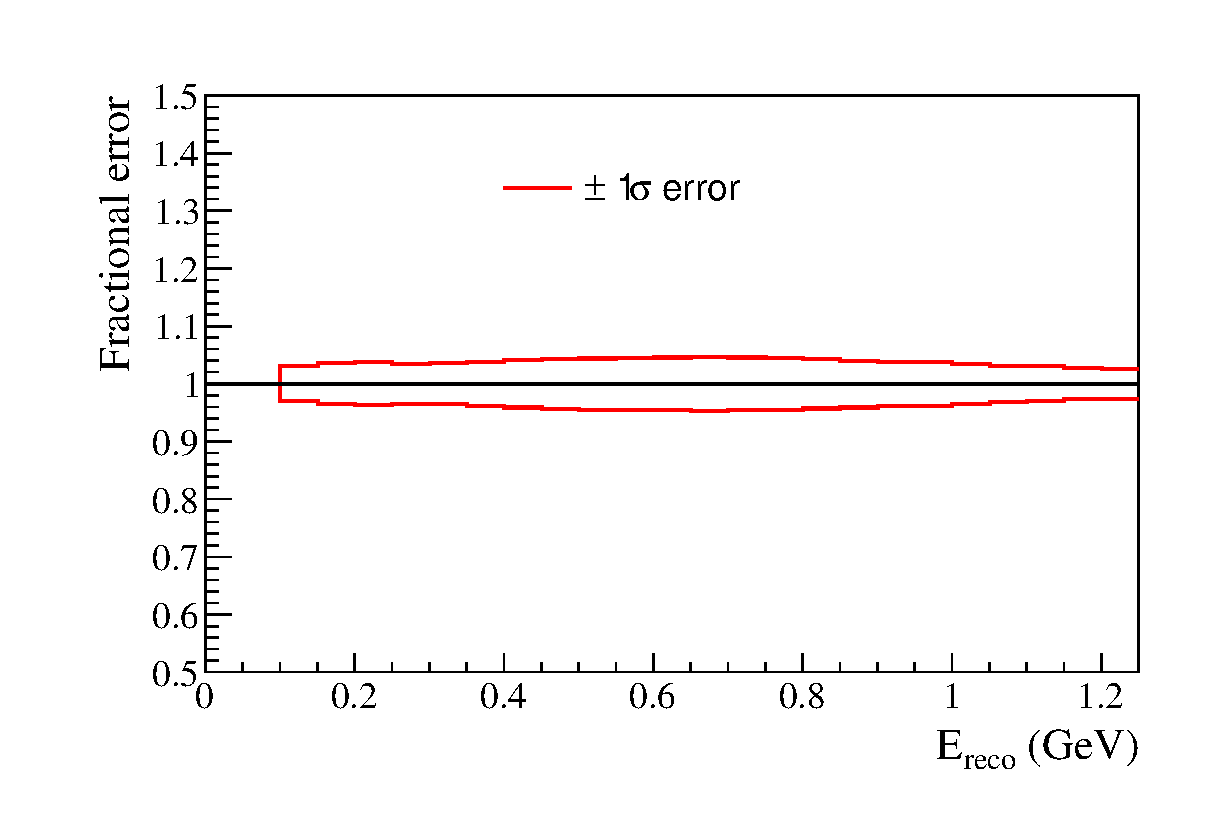
\includegraphics[width=0.9\textwidth]{joint_plots/systematics/Run17c/Asimov_A_1Reoscillated_Osc_param_envelope_ratio.eps}
\caption{Electron-like, neutrino mode}
\end{subfigure}
%rhc e-like
\begin{subfigure}[b]{0.49\textwidth} \centering
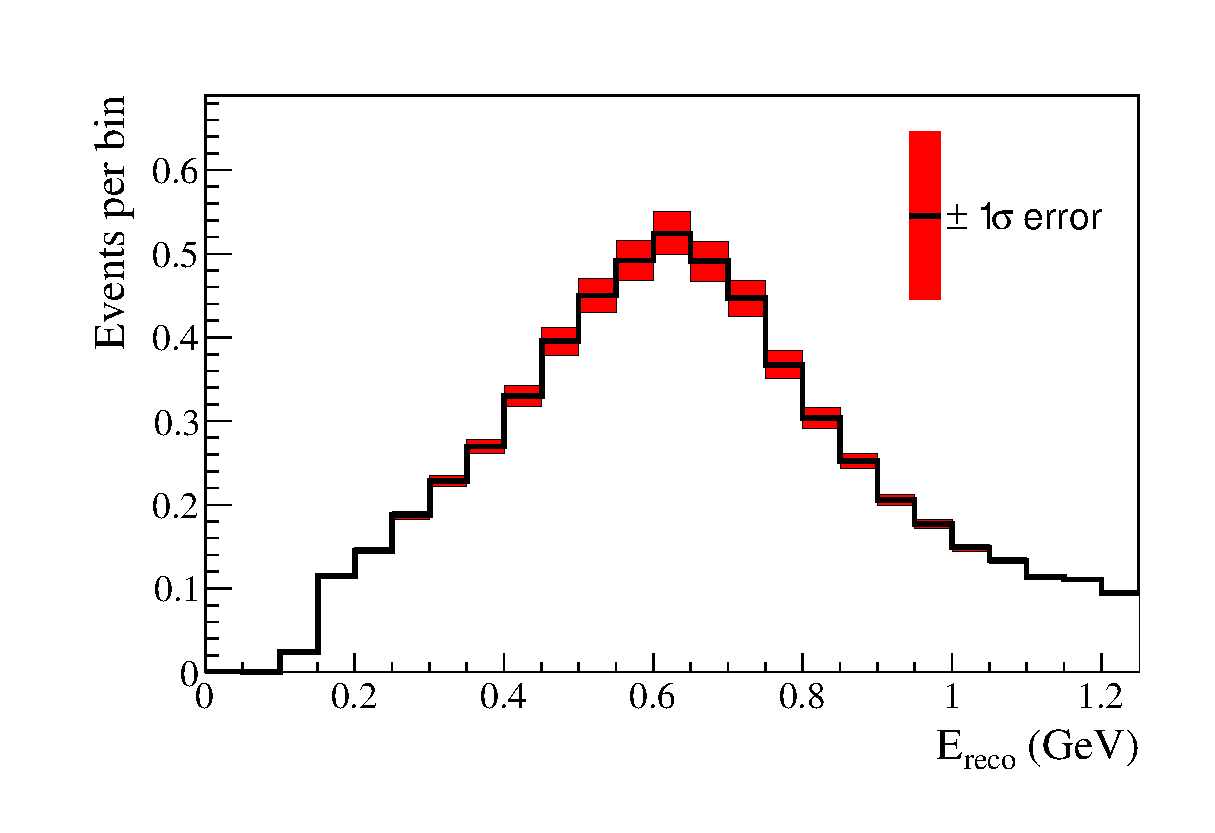
\includegraphics[width=0.9\textwidth]{joint_plots/systematics/Run17c/Asimov_A_RHC1Reoscillated_Osc_param_envelope.eps}
\caption{Electron-like, antineutrino mode}
\end{subfigure}
\begin{subfigure}[b]{0.49\textwidth} \centering
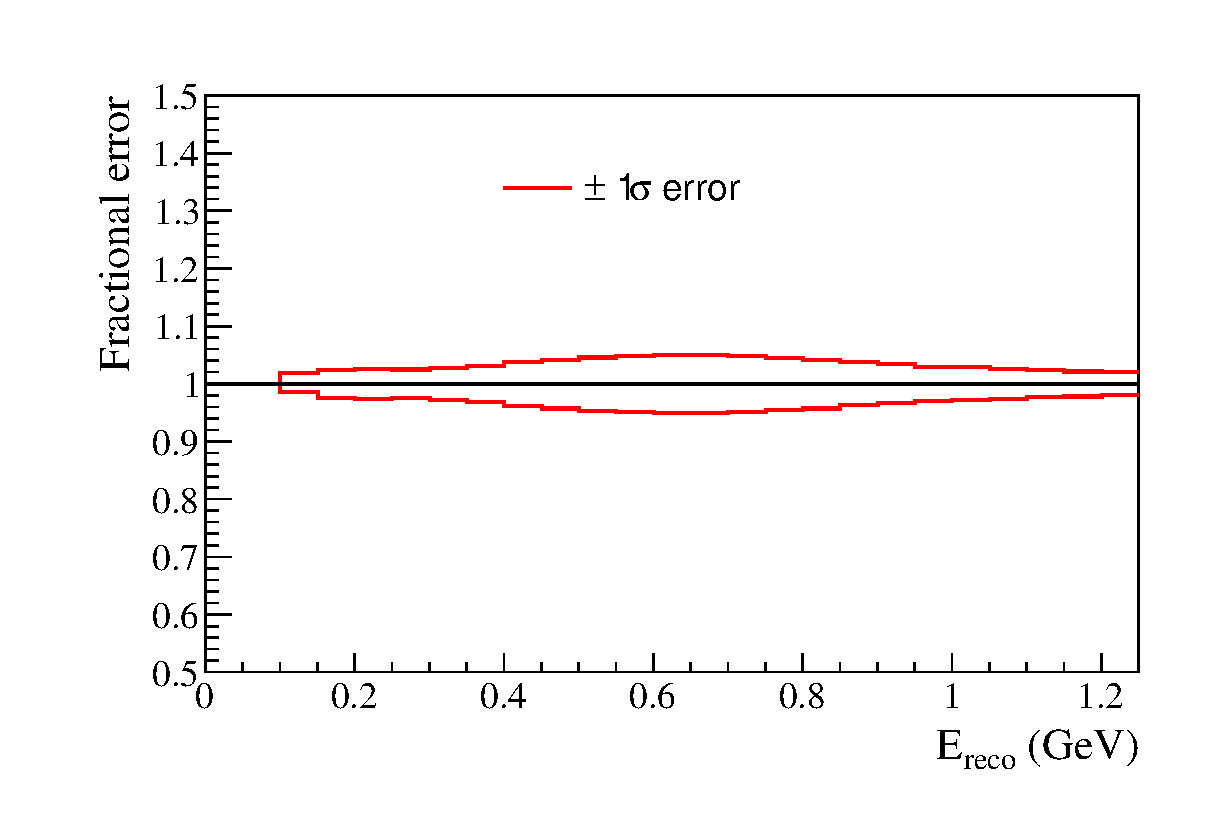
\includegraphics[width=0.9\textwidth]{joint_plots/systematics/Run17c/Asimov_A_RHC1Reoscillated_Osc_param_envelope_ratio.eps} 
\caption{Electron-like, antineutrino mode}
\end{subfigure}
%fhc ccpi-like
\begin{subfigure}[b]{0.49\textwidth} \centering
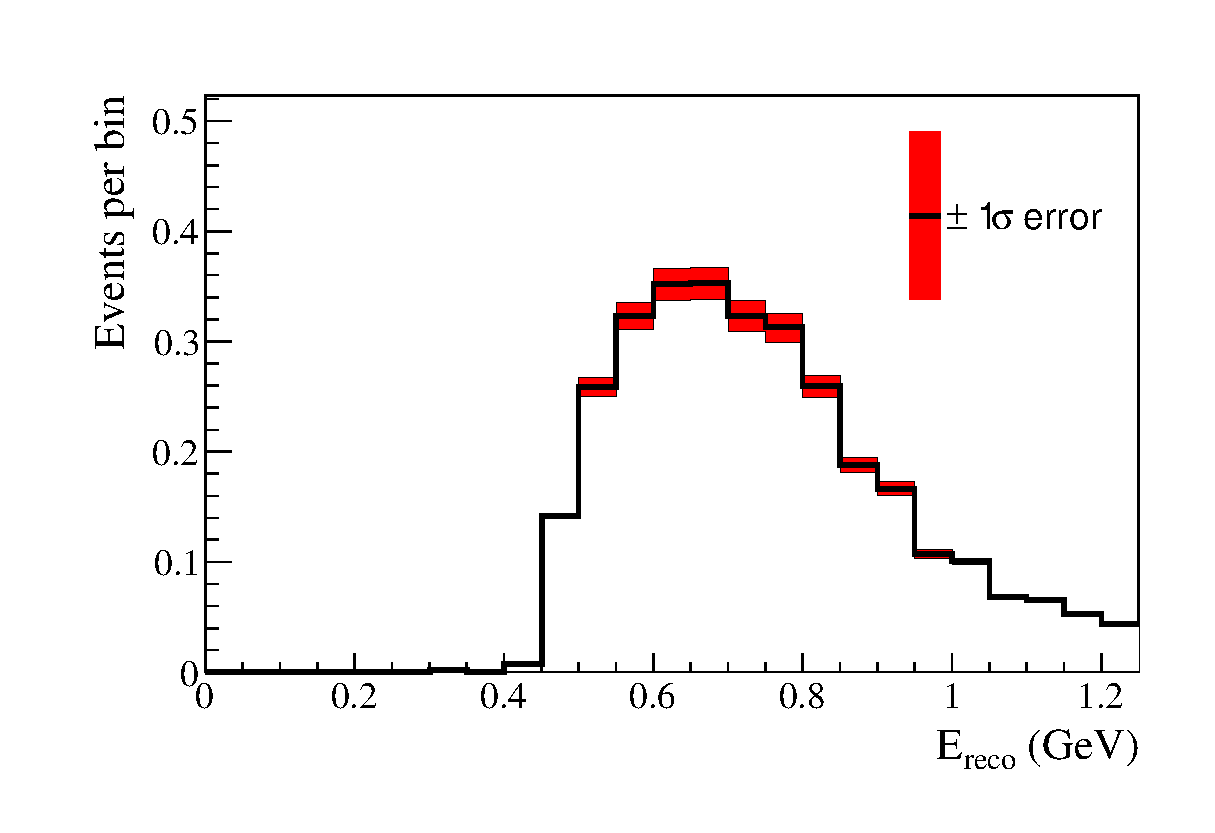
\includegraphics[width=0.9\textwidth]{joint_plots/systematics/Run17c/Asimov_A_MultiReoscillated_Osc_param_envelope.eps} 
\caption{\nueCConepi{}, neutrino mode}
\end{subfigure}
\begin{subfigure}[b]{0.49\textwidth} \centering
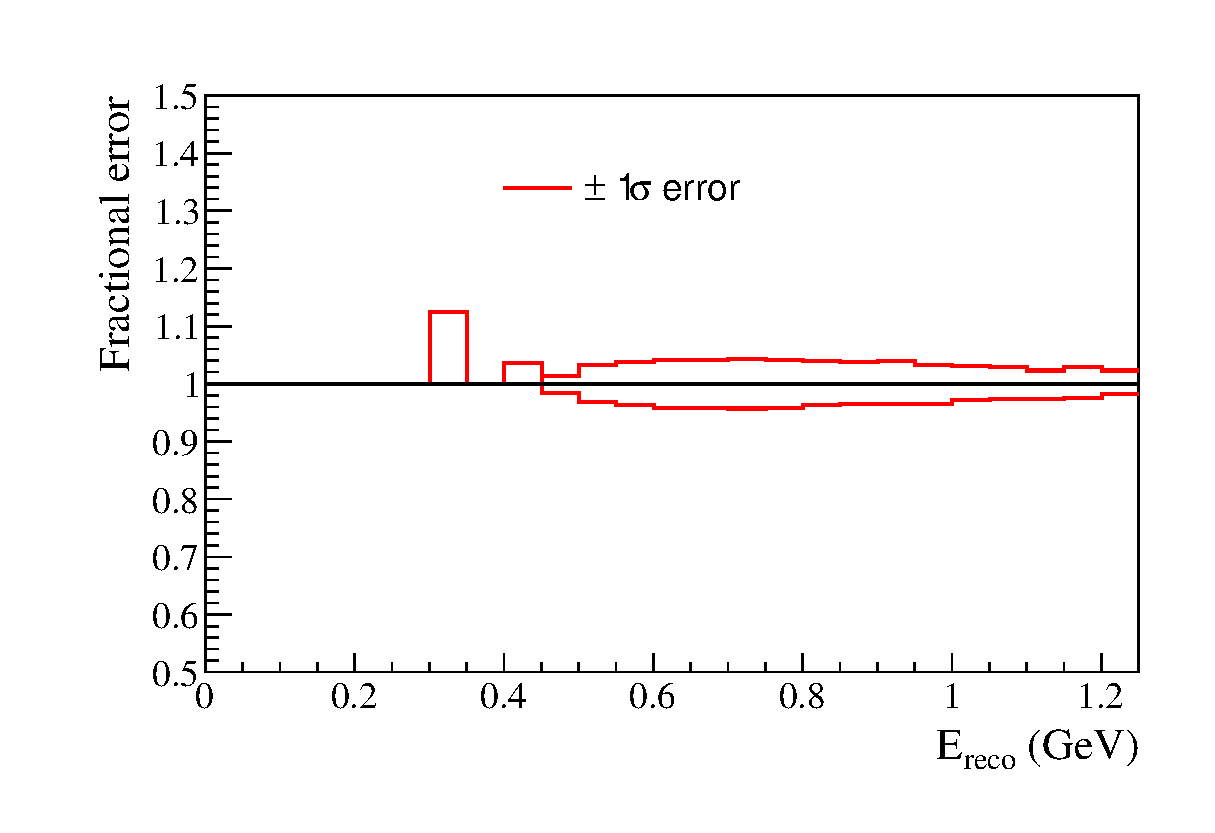
\includegraphics[width=0.9\textwidth]{joint_plots/systematics/Run17c/Asimov_A_MultiReoscillated_Osc_param_envelope_ratio.eps}
\caption{\nueCConepi{}, neutrino mode}
\end{subfigure}
\caption {
Error envelopes (left) and fractional errors (right) for the reconstructed neutrino energy spectrum
as a result of the oscillation systematic parameters.
10k toy MC experiments are generated for the Asimov data set A shown in \cref{tab:osc_params_joint_asimov}
with randomised systematic parameters, taking into account their correlations.
Since the parameters $\delta_{CP}$, $\theta_{23}$ and $\Delta m^2_{32}$ ($\Delta m^2_{13}$) and mass hierarchy
will be measured,
only the uncertainty on 
$\sin^2 \theta_{13}$,
$\sin^2 \theta_{12}$
and 
$\Delta m^2_{21}$ 
are taken into account.
BANFF tuned MC templates are used. 
The distributions correspond to the collected statistics in the full Run 1-7c data set.
The changes due to the Run 1-7c flux and covariance matrix updates are applied.
}
\label{fig:Osc_envelope_Asimov_A_run17c_elike}
\end{figure*}


\begin{figure*}[htb]
\center
%fhc mu-like
\begin{subfigure}[b]{0.49\textwidth} \centering
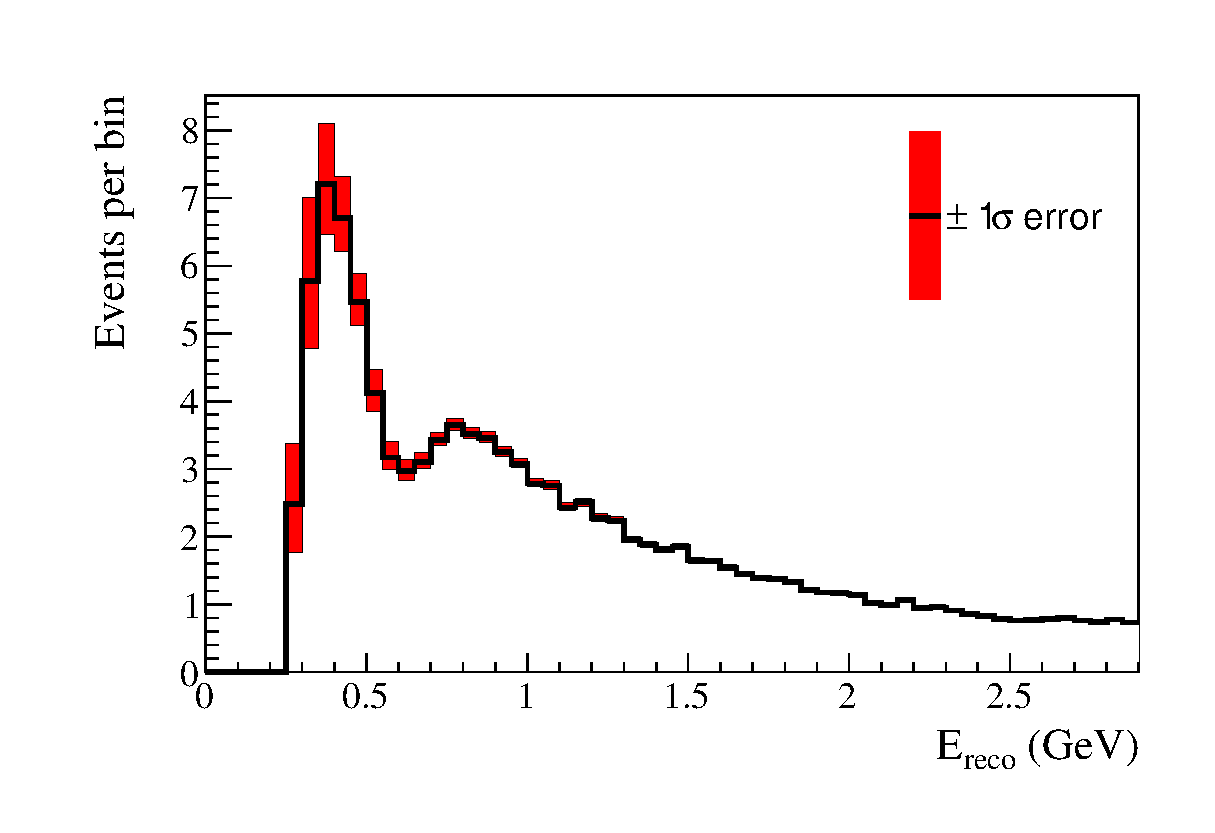
\includegraphics[width=0.9\textwidth]{joint_plots/systematics/Run17c/Asimov_A_1Rmuoscillated_SKDet_FSI_envelope.eps} 
\caption{Muon-like, neutrino mode}
\end{subfigure}
\begin{subfigure}[b]{0.49\textwidth} \centering
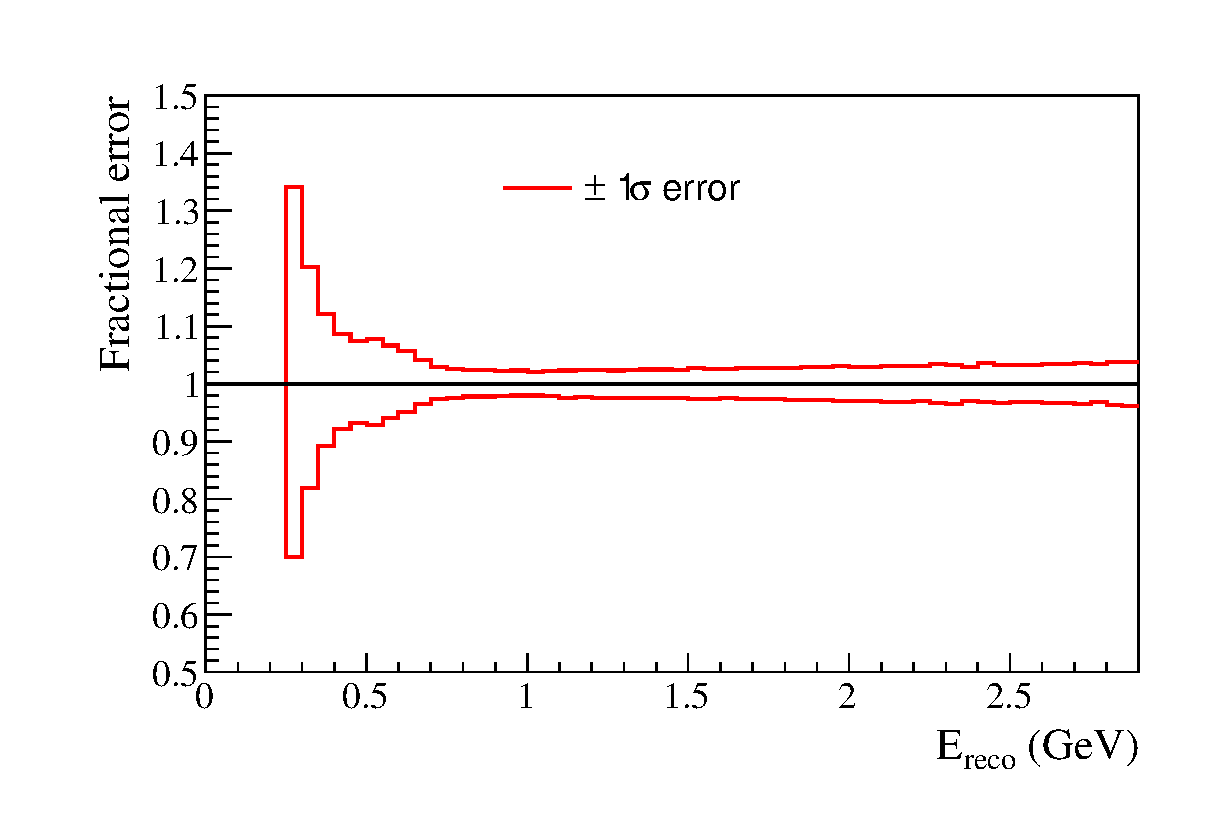
\includegraphics[width=0.9\textwidth]{joint_plots/systematics/Run17c/Asimov_A_1Rmuoscillated_SKDet_FSI_envelope_ratio.eps} 
\caption{Muon-like, neutrino mode}
\end{subfigure}
%rhc mu-like
\begin{subfigure}[b]{0.49\textwidth} \centering
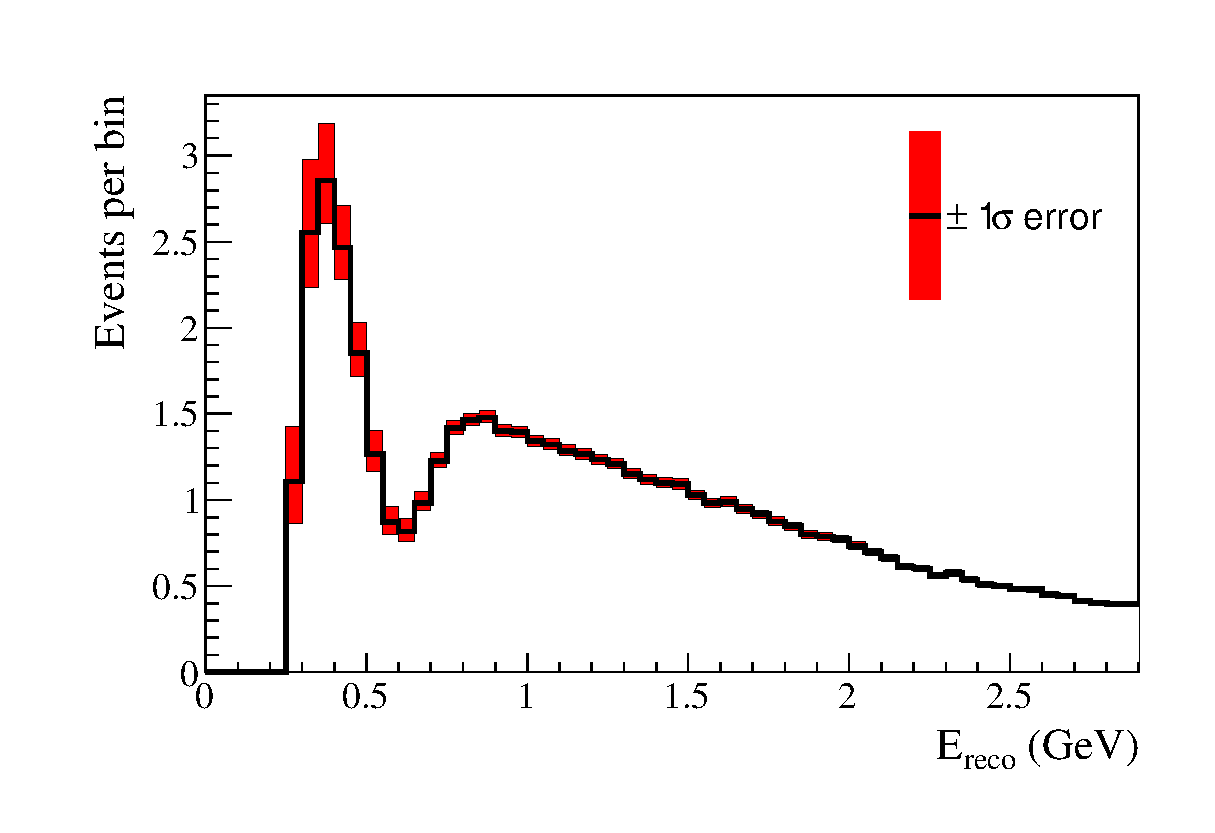
\includegraphics[width=0.9\textwidth]{joint_plots/systematics/Run17c/Asimov_A_RHC1Rmuoscillated_SKDet_FSI_envelope.eps} \\ 
\caption{Muon-like, antineutrino mode}
\end{subfigure}
\begin{subfigure}[b]{0.49\textwidth} \centering
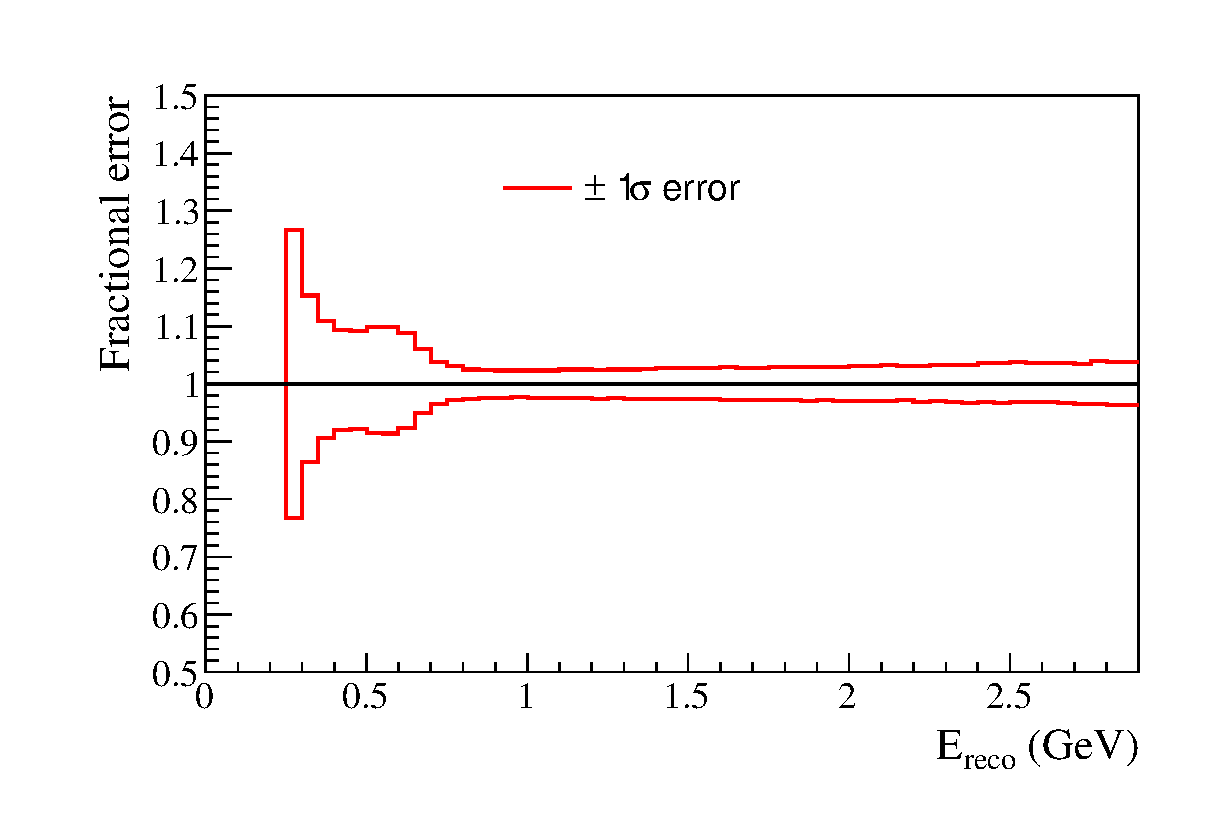
\includegraphics[width=0.9\textwidth]{joint_plots/systematics/Run17c/Asimov_A_RHC1Rmuoscillated_SKDet_FSI_envelope_ratio.eps} \\ 
\caption{Muon-like, antineutrino mode}
\end{subfigure}
%fhc e-like
\caption {
Error envelopes (left) and fractional errors (right) for the reconstructed neutrino energy spectrum
as a result of the Super-K + FSI + SI + PN systematic parameters.
	10k toy MC experiments are generated for the Asimov data set A shown in \cref{tab:osc_params_joint_asimov}
	with random systematic parameters, taking into account their correlations.
	Since the parameters $\delta_{CP}$, $\theta_{23}$ and $\Delta m^2_{32}$ ($\Delta m^2_{13}$) and mass hierarchy
will be measured,
only the uncertainty on 
$\sin^2 \theta_{13}$,
$\sin^2 \theta_{12}$
and 
$\Delta m^2_{21}$ 
are taken into account.
BANFF tuned MC templates are used. 
The distributions correspond to the collected statistics in the full Run 1-7c data set.
The changes due to the Run 1-7c flux and covariance matrix updates are applied.
}
\label{fig:SKDet_FSI_envelope_Asimov_A_run17c_mulike}
\end{figure*}


\begin{figure*}[htb]
\center

\begin{subfigure}[b]{0.49\textwidth} \centering
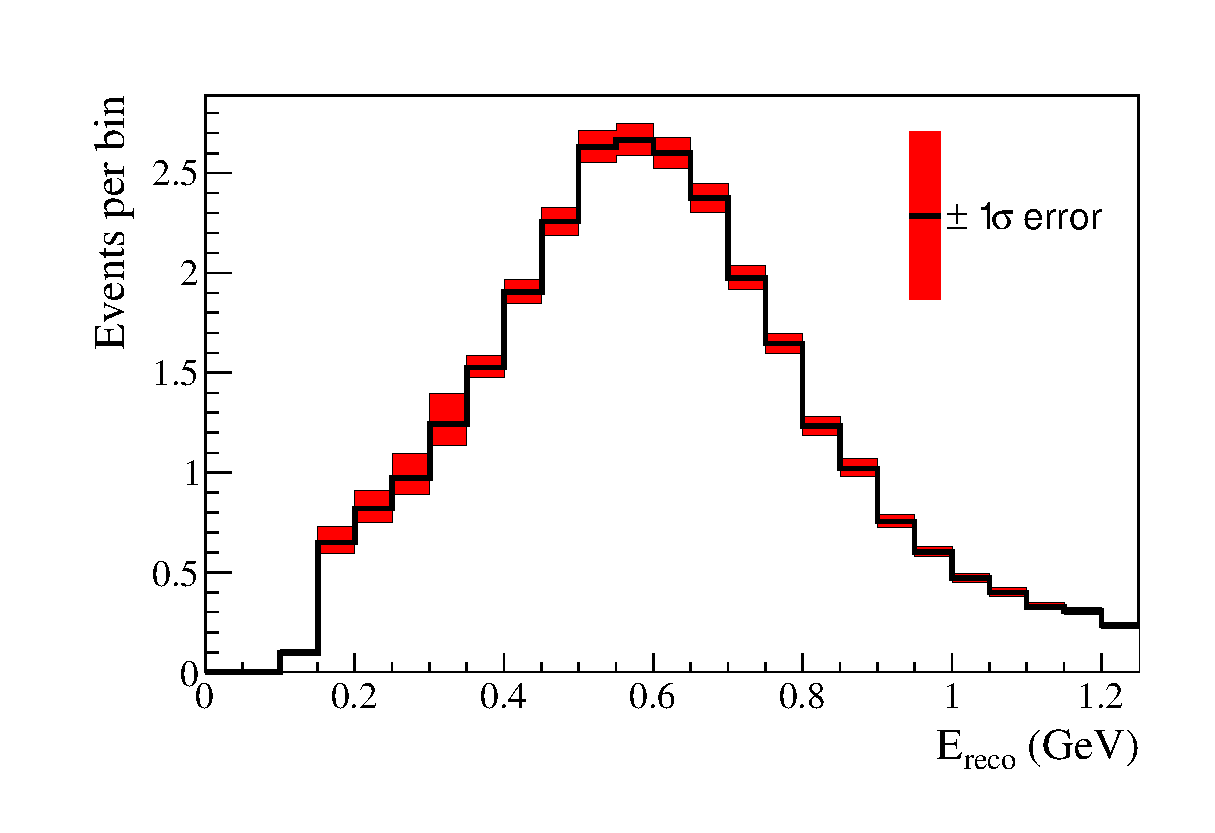
\includegraphics[width=0.9\textwidth]{joint_plots/systematics/Run17c/Asimov_A_1Reoscillated_SKDet_FSI_envelope.eps} 
\caption{Electron-like, neutrino mode}
\end{subfigure}
\begin{subfigure}[b]{0.49\textwidth} \centering
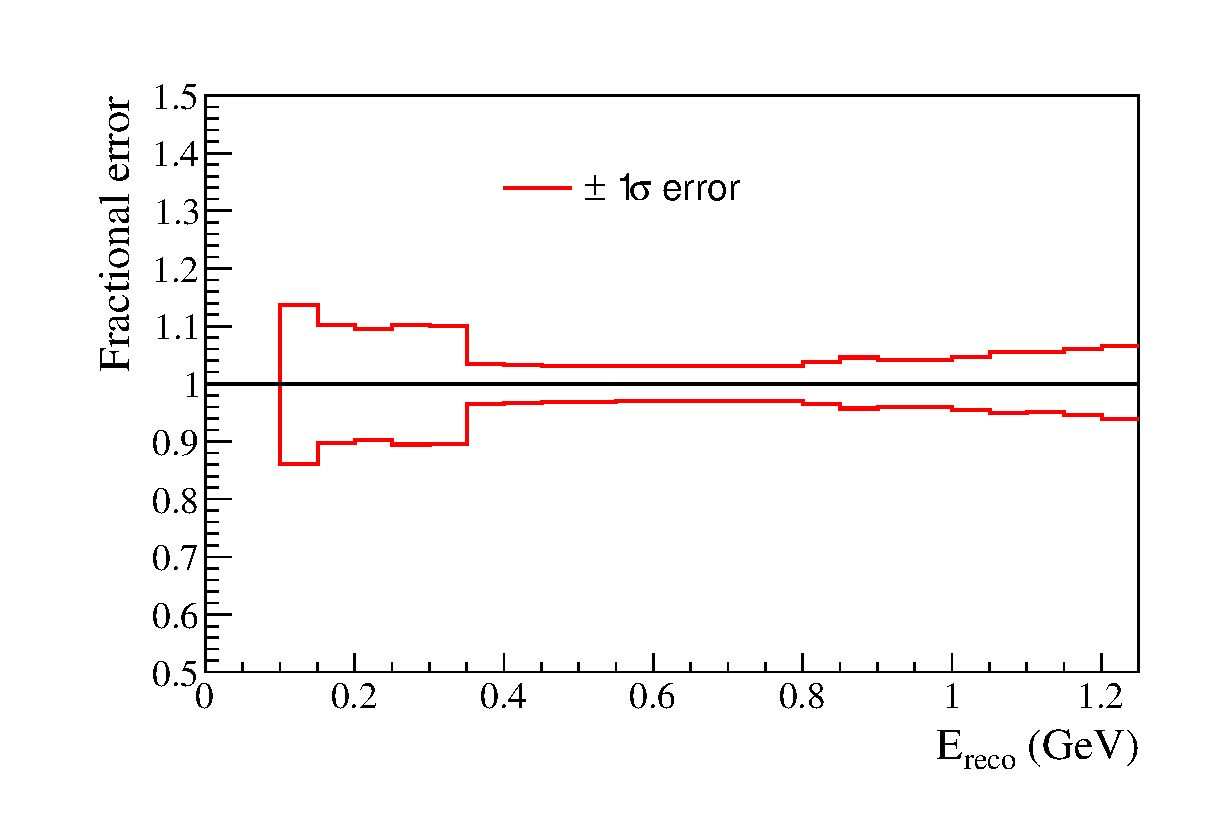
\includegraphics[width=0.9\textwidth]{joint_plots/systematics/Run17c/Asimov_A_1Reoscillated_SKDet_FSI_envelope_ratio.eps} 
\caption{Electron-like, neutrino mode}
\end{subfigure}
%rhc e-like
\begin{subfigure}[b]{0.49\textwidth} \centering
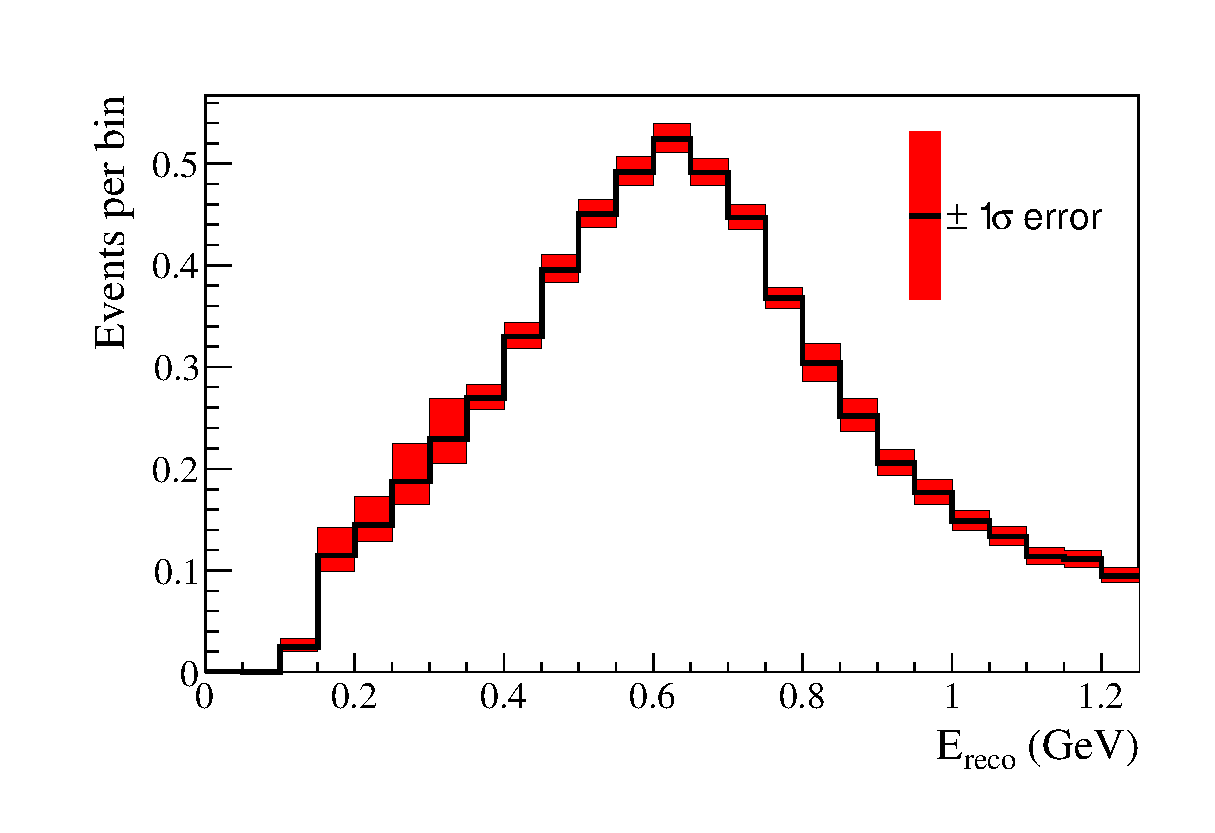
\includegraphics[width=0.9\textwidth]{joint_plots/systematics/Run17c/Asimov_A_RHC1Reoscillated_SKDet_FSI_envelope.eps} 
\caption{Electron-like, antineutrino mode}
\end{subfigure}
\begin{subfigure}[b]{0.49\textwidth} \centering
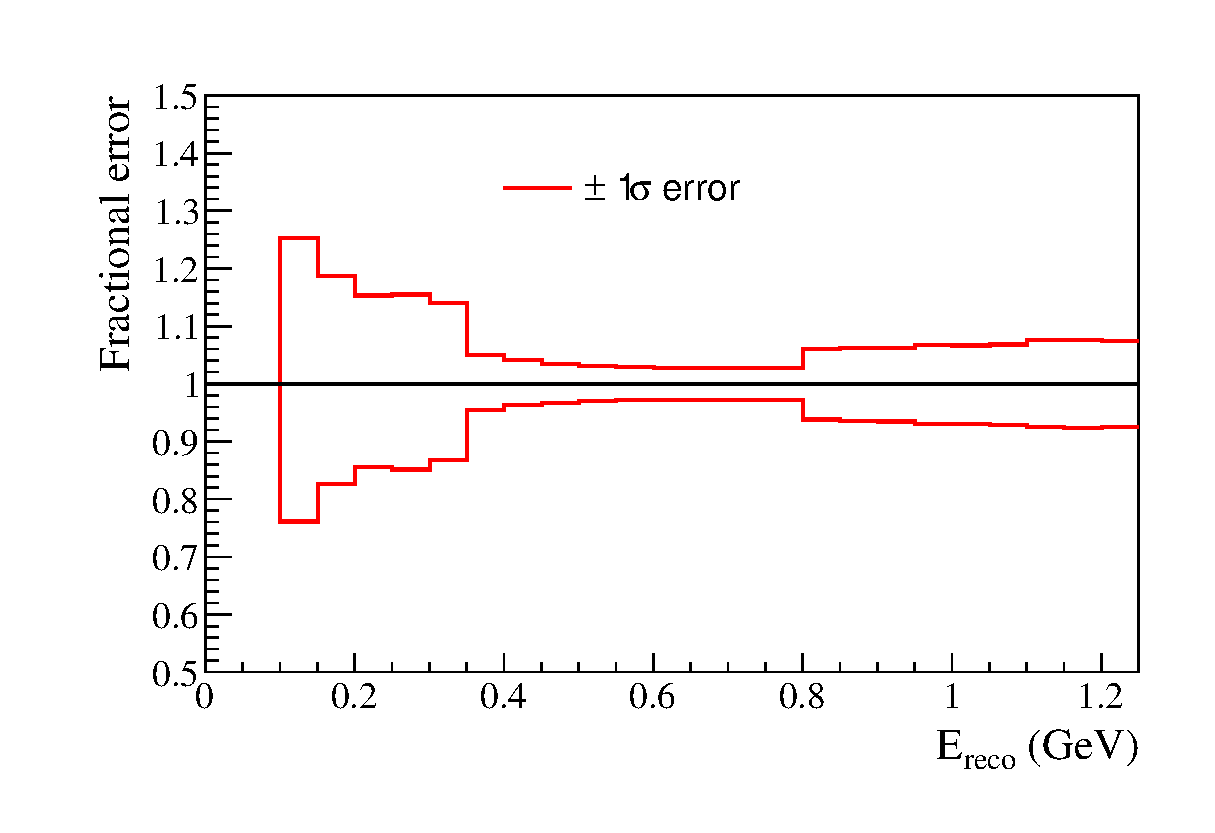
\includegraphics[width=0.9\textwidth]{joint_plots/systematics/Run17c/Asimov_A_RHC1Reoscillated_SKDet_FSI_envelope_ratio.eps} 
\caption{Electron-like, antineutrino mode}
\end{subfigure}
%fhc ccpi-like
\begin{subfigure}[b]{0.49\textwidth} \centering
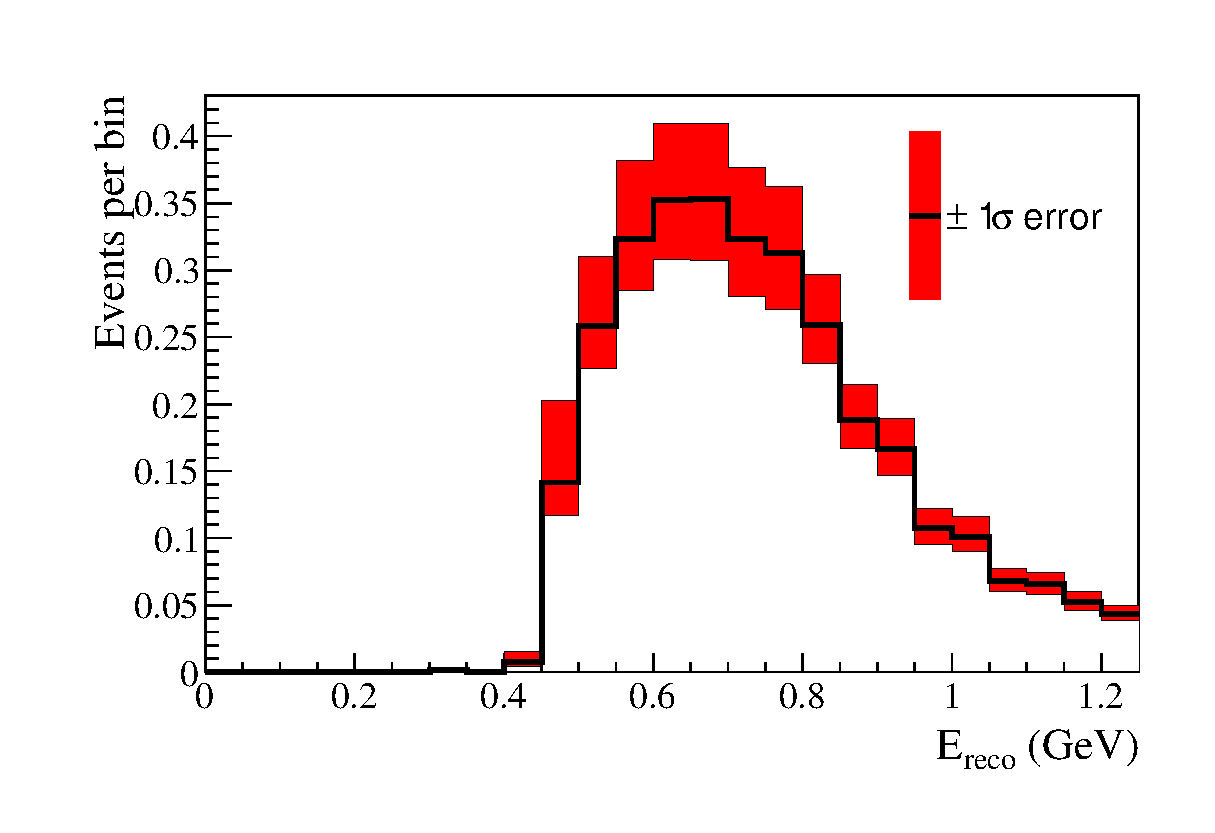
\includegraphics[width=0.9\textwidth]{joint_plots/systematics/Run17c/Asimov_A_MultiReoscillated_SKDet_FSI_envelope.eps} 
\caption{\nueCConepi{}, neutrino mode}
\end{subfigure}
\begin{subfigure}[b]{0.49\textwidth} \centering
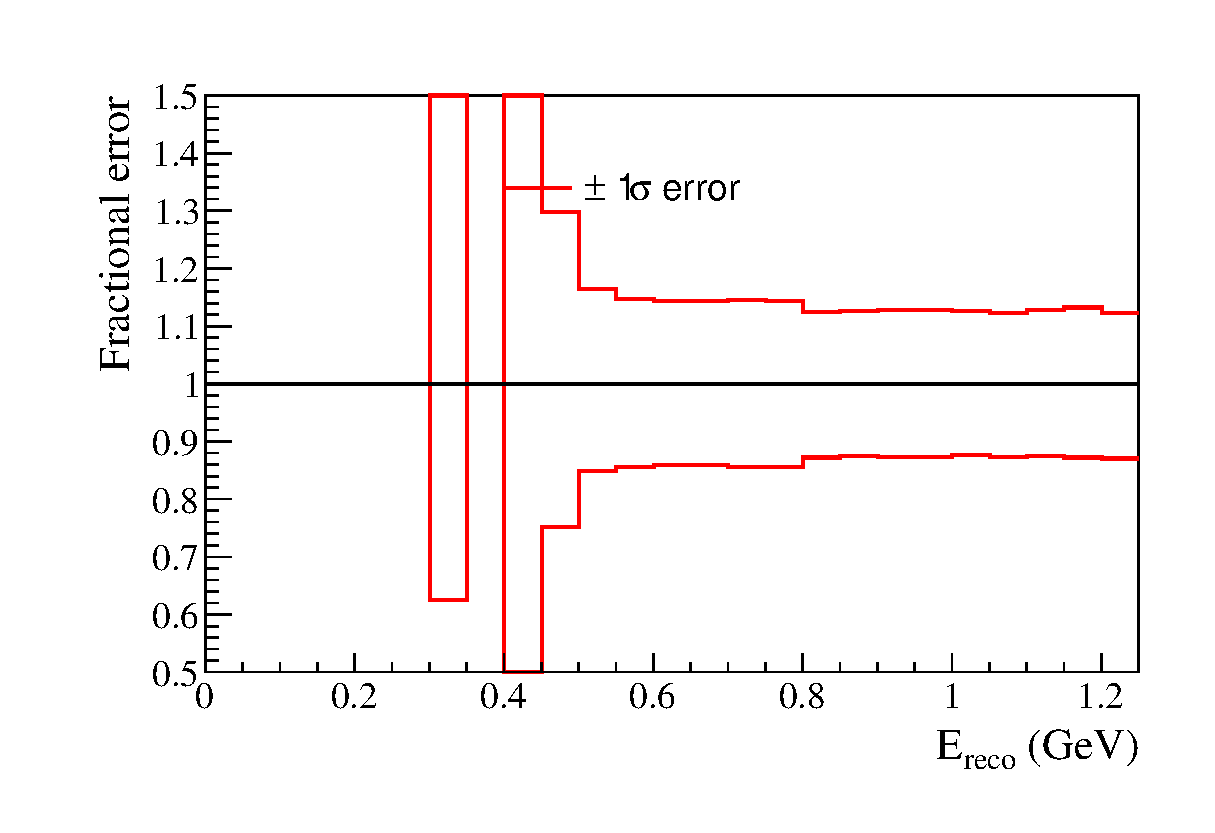
\includegraphics[width=0.9\textwidth]{joint_plots/systematics/Run17c/Asimov_A_MultiReoscillated_SKDet_FSI_envelope_ratio.eps} 
\caption{\nueCConepi{}, neutrino mode}
\end{subfigure}
\caption {
Error envelopes (left) and fractional errors (right) for the reconstructed neutrino energy spectrum
as a result of the Super-K + FSI + SI + PN systematic parameters.
10k toy MC experiments are generated for the Asimov data set A shown in \cref{tab:osc_params_joint_asimov}
with randomised systematic parameters, taking into account their correlations.
Since the parameters $\delta_{CP}$, $\theta_{23}$ and $\Delta m^2_{32}$ ($\Delta m^2_{13}$) and mass hierarchy
will be measured,
only the uncertainty on 
$\sin^2 \theta_{13}$,
$\sin^2 \theta_{12}$
and 
$\Delta m^2_{21}$ 
are taken into account.
BANFF tuned MC templates are used. 
The distributions correspond to the collected statistics in the full Run 1-7c data set.
The changes due to the Run 1-7c flux and covariance matrix updates are applied.
}
\label{fig:SKDet_FSI_envelope_Asimov_A_run17c_elike}
\end{figure*}




\begin{figure*}[htb]
\center
%fhc mu-like
\begin{subfigure}[b]{0.49\textwidth} \centering
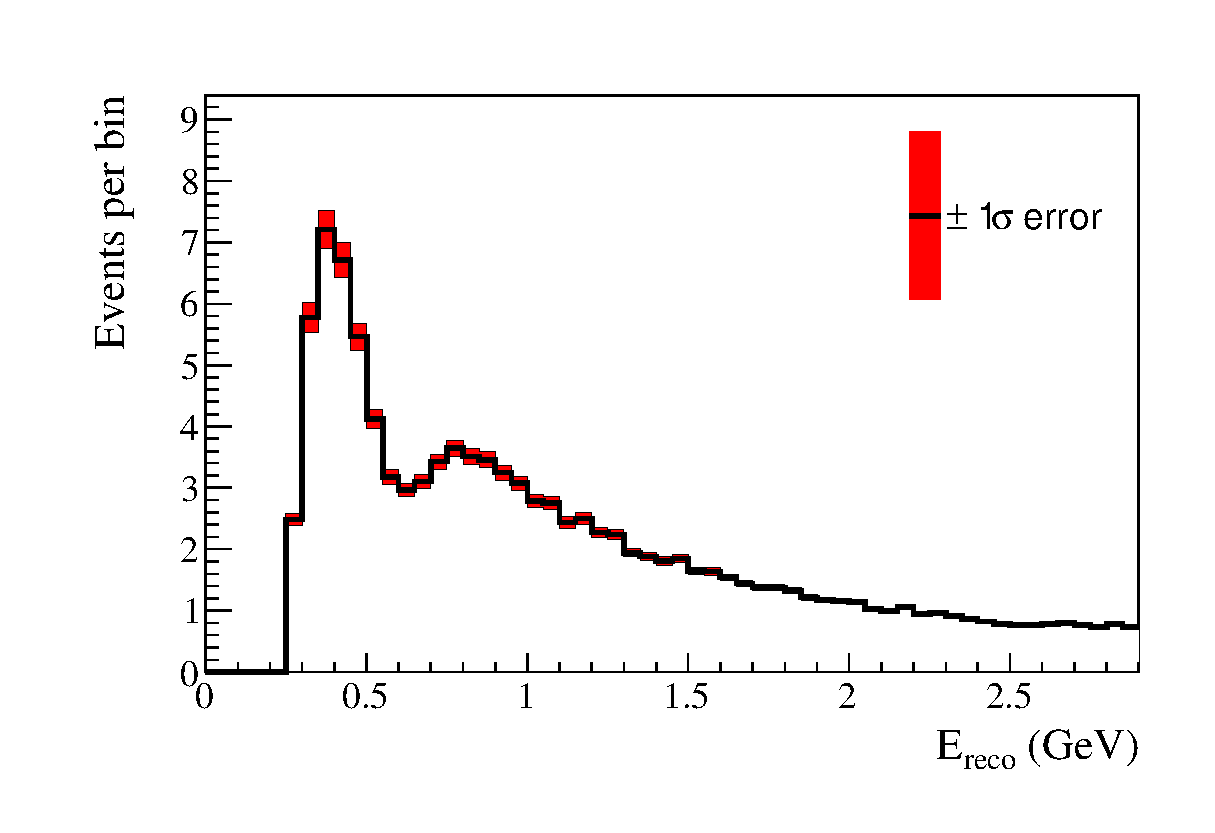
\includegraphics[width=0.9\textwidth]{joint_plots/systematics/Run17c/Asimov_A_1Rmuoscillated_BANFF_flux_envelope.eps} 
\caption{Muon-like, neutrino mode}
\end{subfigure}
\begin{subfigure}[b]{0.49\textwidth} \centering
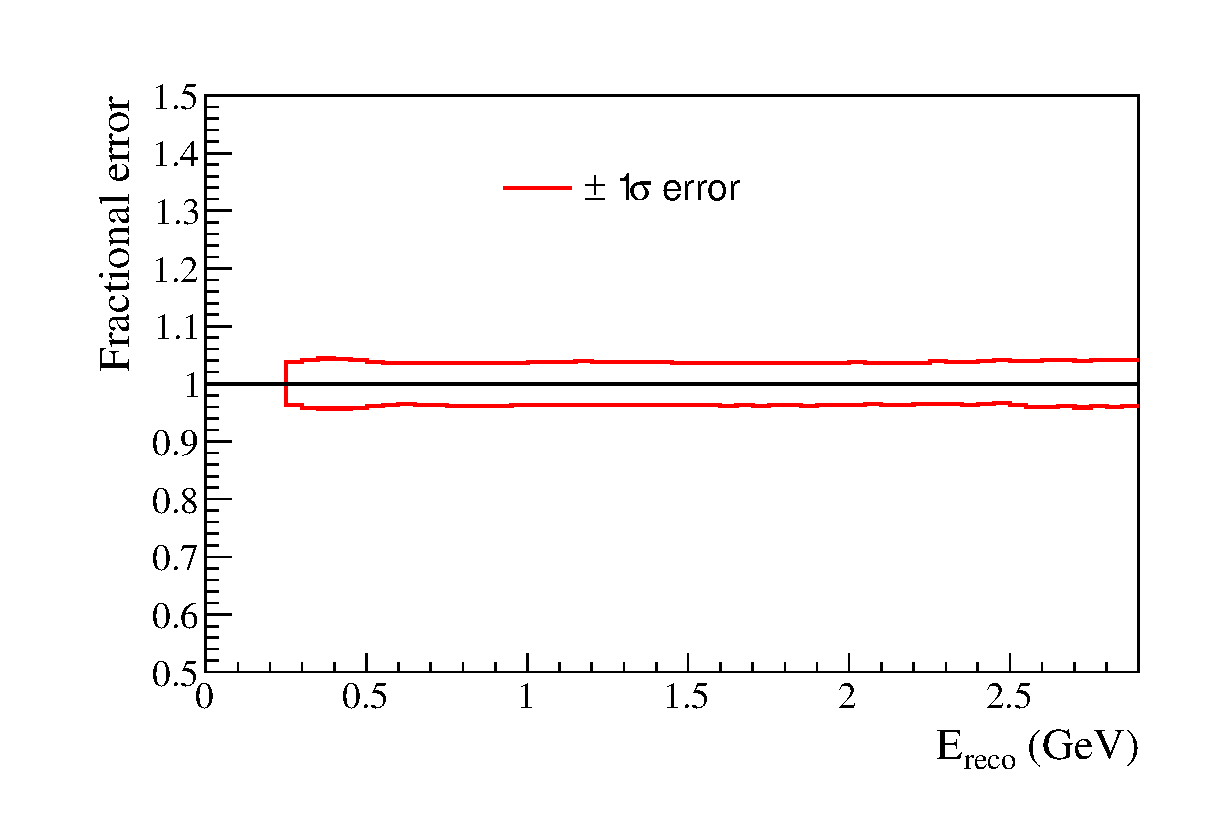
\includegraphics[width=0.9\textwidth]{joint_plots/systematics/Run17c/Asimov_A_1Rmuoscillated_BANFF_flux_envelope_ratio.eps} 
\caption{Muon-like, neutrino mode}
\end{subfigure}
%rhc mu-like
\begin{subfigure}[b]{0.49\textwidth} \centering
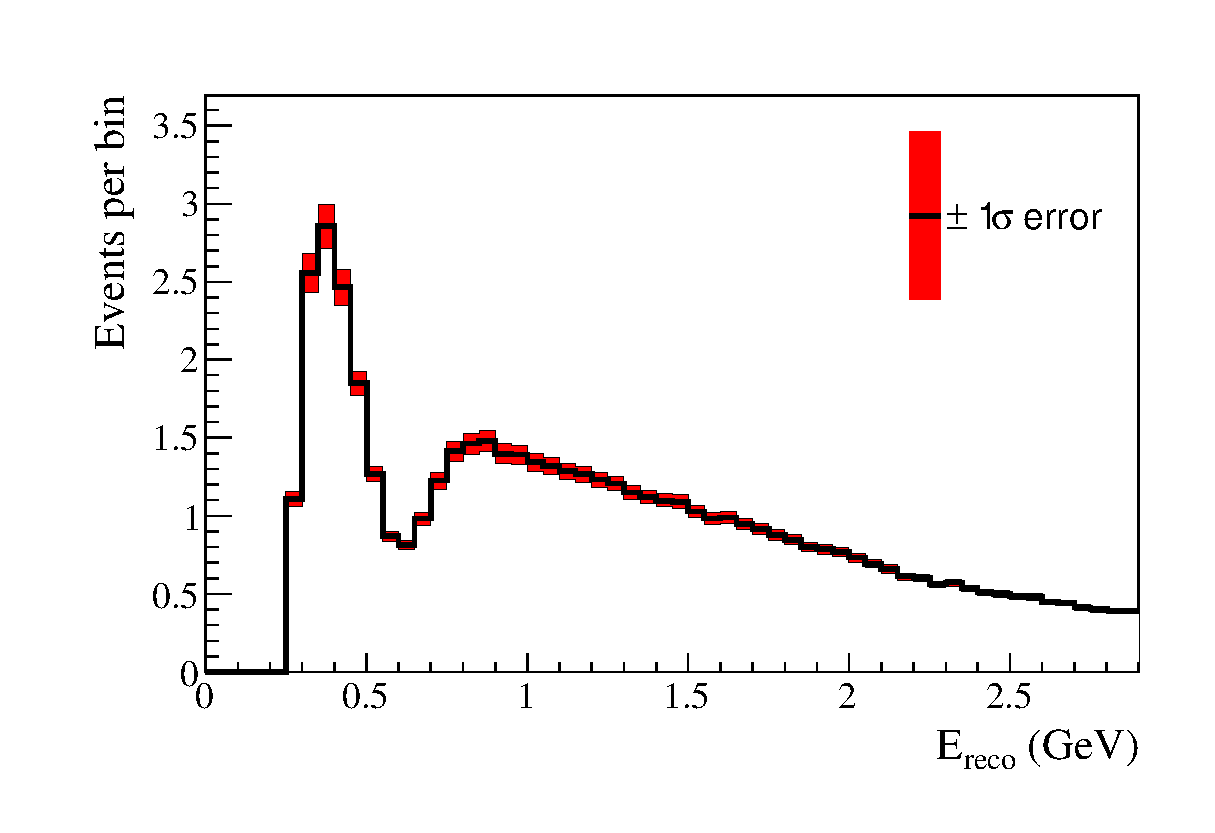
\includegraphics[width=0.9\textwidth]{joint_plots/systematics/Run17c/Asimov_A_RHC1Rmuoscillated_BANFF_flux_envelope.eps} \\ 
\caption{Muon-like, antineutrino mode}
\end{subfigure}
\begin{subfigure}[b]{0.49\textwidth} \centering
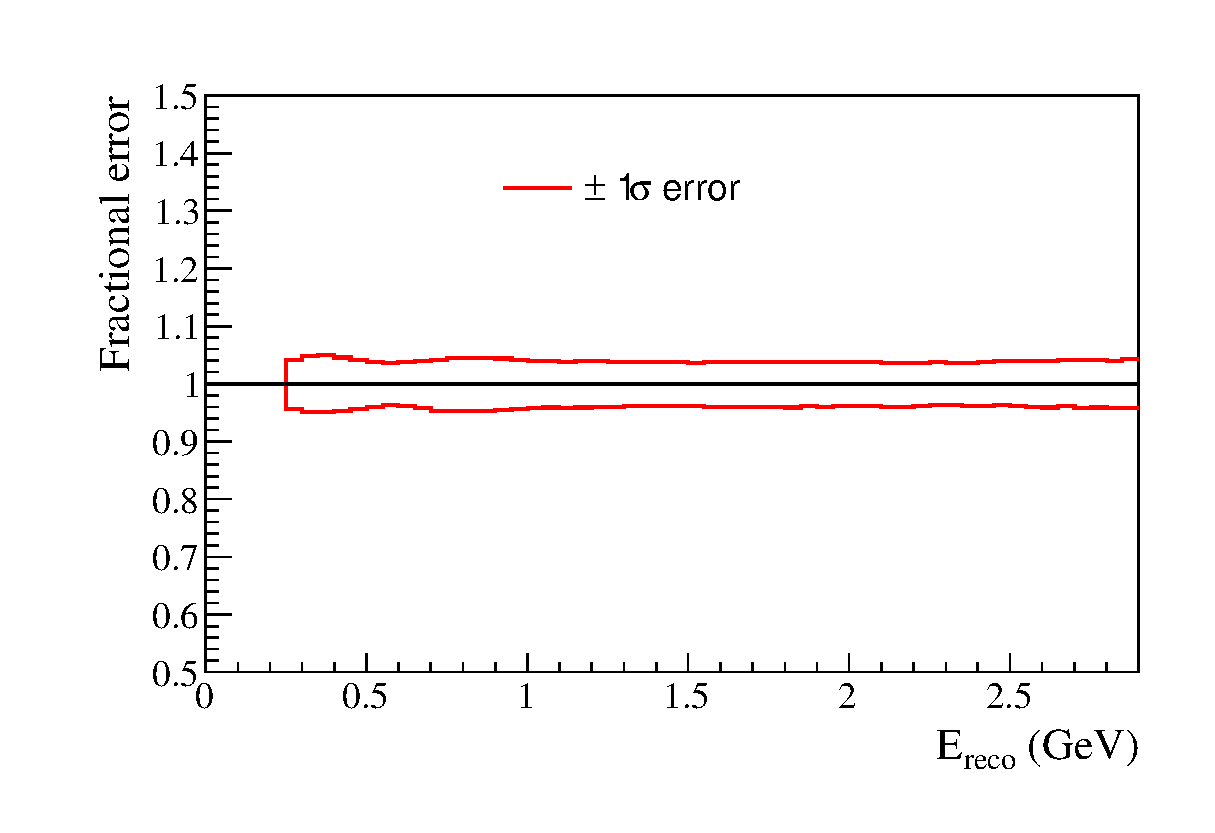
\includegraphics[width=0.9\textwidth]{joint_plots/systematics/Run17c/Asimov_A_RHC1Rmuoscillated_BANFF_flux_envelope_ratio.eps} \\ 
\caption{Muon-like, antineutrino mode}
\end{subfigure}
%fhc e-like
\caption {
Error envelopes (left) and fractional errors (right) for the reconstructed neutrino energy spectrum
as a result of the flux systematic parameters.
	10k toy MC experiments are generated for the Asimov data set A shown in \cref{tab:osc_params_joint_asimov}
	with random systematic parameters, taking into account their correlations.
	Since the parameters $\delta_{CP}$, $\theta_{23}$ and $\Delta m^2_{32}$ ($\Delta m^2_{13}$) and mass hierarchy
will be measured,
only the uncertainty on 
$\sin^2 \theta_{13}$,
$\sin^2 \theta_{12}$
and 
$\Delta m^2_{21}$ 
are taken into account.
BANFF tuned MC templates are used. 
The distributions correspond to the collected statistics in the full Run 1-7c data set.
The changes due to the Run 1-7c flux and covariance matrix updates are applied.
}
\label{fig:flux_envelope_Asimov_A_run17c_mulike}
\end{figure*}


\begin{figure*}[htb]
\center

\begin{subfigure}[b]{0.49\textwidth} \centering
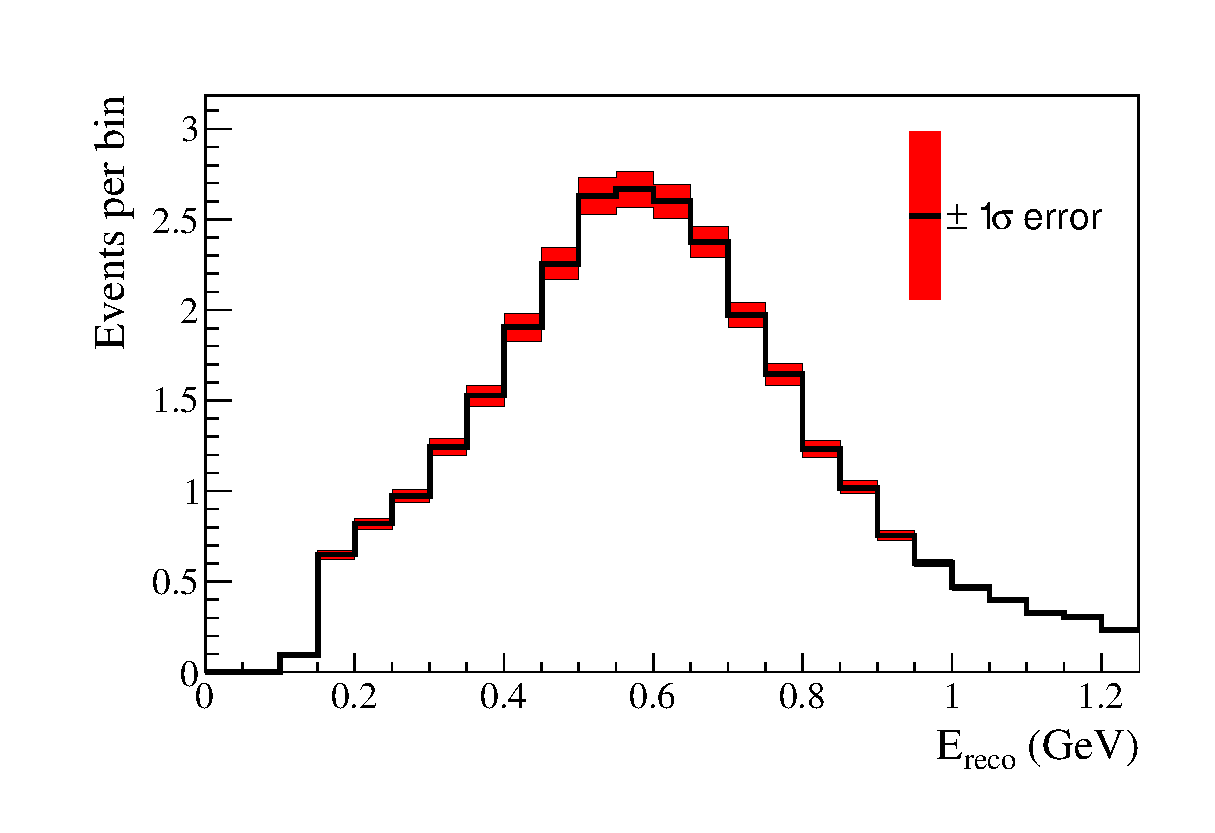
\includegraphics[width=0.9\textwidth]{joint_plots/systematics/Run17c/Asimov_A_1Reoscillated_BANFF_flux_envelope.eps} 
\caption{Electron-like, neutrino mode}
\end{subfigure}
\begin{subfigure}[b]{0.49\textwidth} \centering
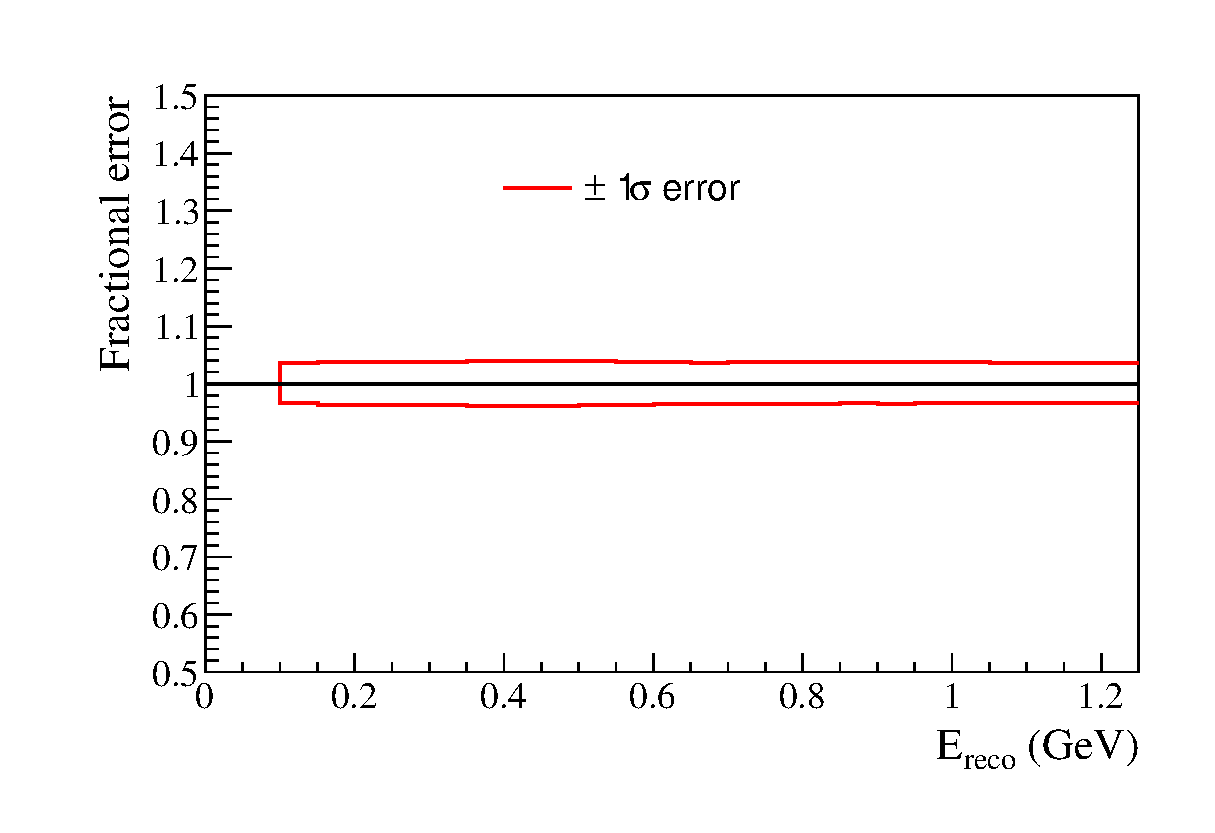
\includegraphics[width=0.9\textwidth]{joint_plots/systematics/Run17c/Asimov_A_1Reoscillated_BANFF_flux_envelope_ratio.eps} 
\caption{Electron-like, neutrino mode}
\end{subfigure}
%rhc e-like
\begin{subfigure}[b]{0.49\textwidth} \centering
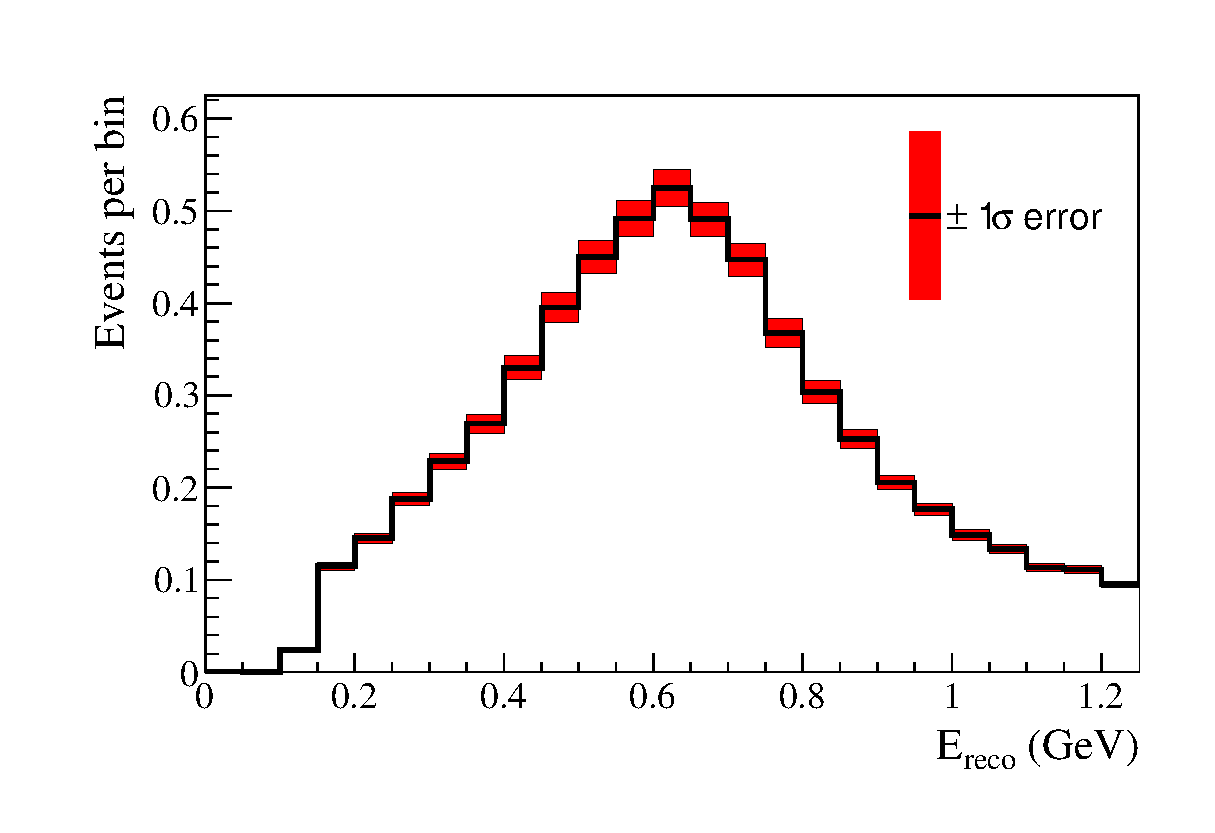
\includegraphics[width=0.9\textwidth]{joint_plots/systematics/Run17c/Asimov_A_RHC1Reoscillated_BANFF_flux_envelope.eps} 
\caption{Electron-like, antineutrino mode}
\end{subfigure}
\begin{subfigure}[b]{0.49\textwidth} \centering
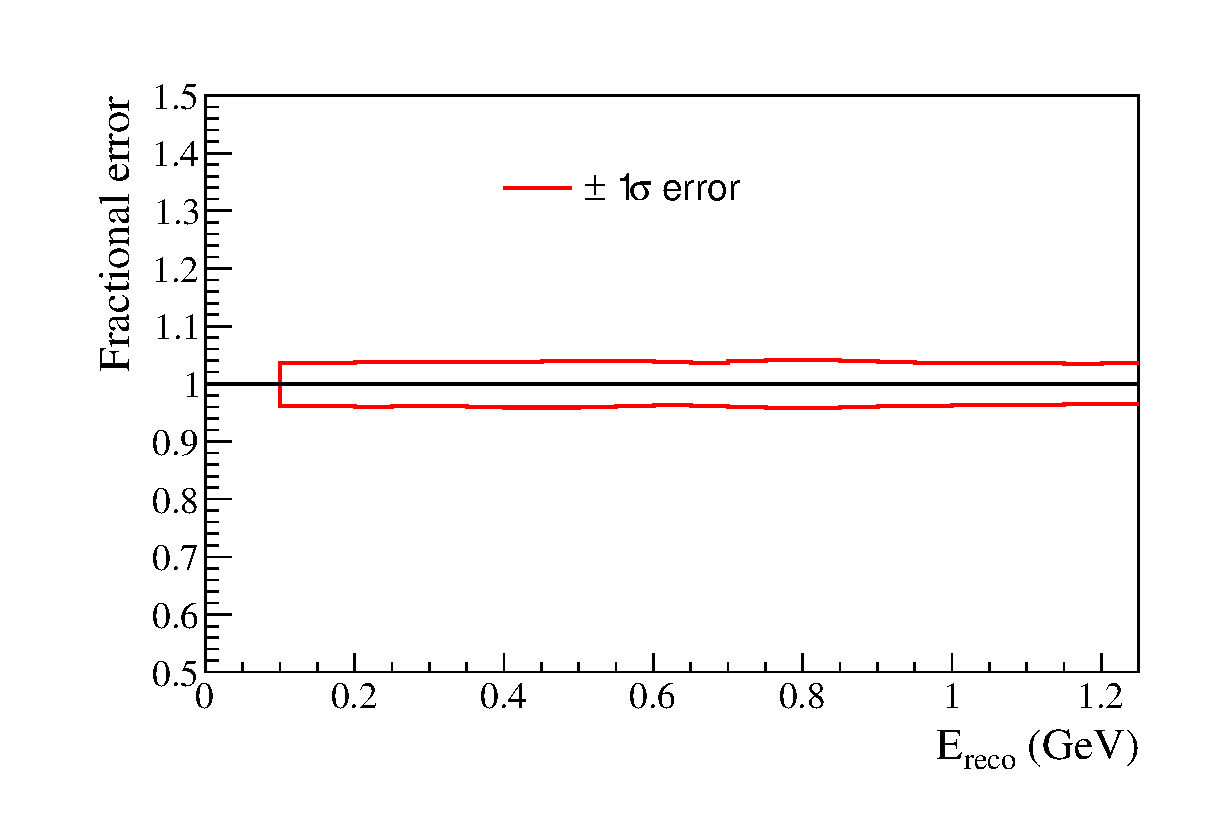
\includegraphics[width=0.9\textwidth]{joint_plots/systematics/Run17c/Asimov_A_RHC1Reoscillated_BANFF_flux_envelope_ratio.eps} 
\caption{Electron-like, antineutrino mode}
\end{subfigure}
%fhc ccpi-like
\begin{subfigure}[b]{0.49\textwidth} \centering
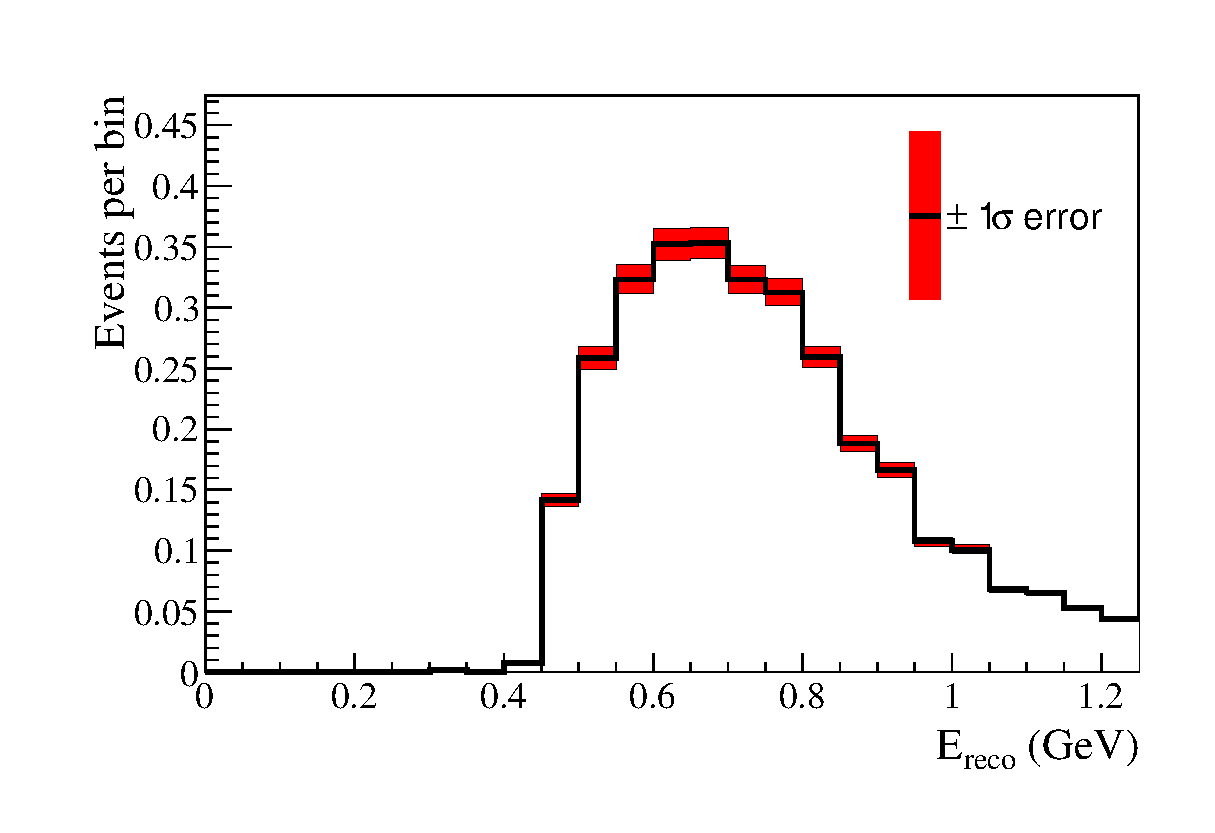
\includegraphics[width=0.9\textwidth]{joint_plots/systematics/Run17c/Asimov_A_MultiReoscillated_BANFF_flux_envelope.eps} 
\caption{\nueCConepi{}, neutrino mode}
\end{subfigure}
\begin{subfigure}[b]{0.49\textwidth} \centering
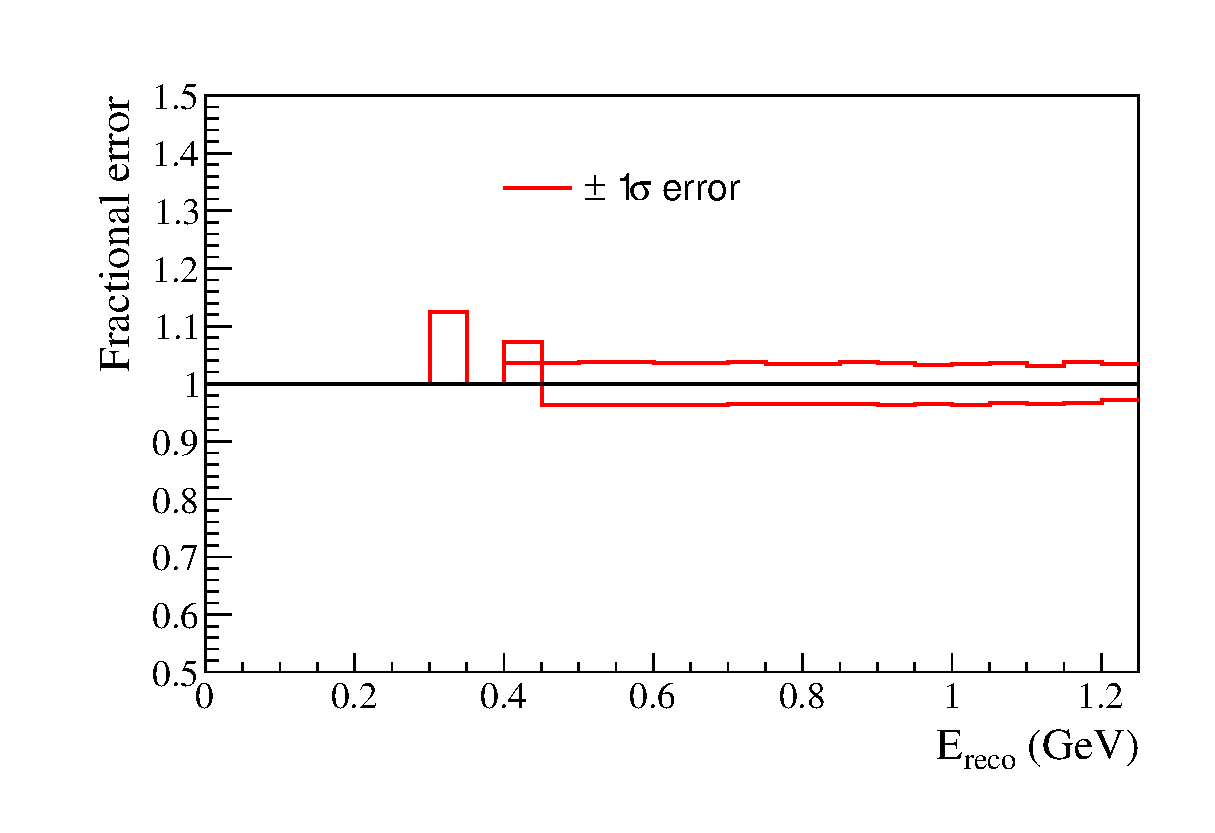
\includegraphics[width=0.9\textwidth]{joint_plots/systematics/Run17c/Asimov_A_MultiReoscillated_BANFF_flux_envelope_ratio.eps} 
\caption{\nueCConepi{}, neutrino mode}
\end{subfigure}
\caption {
Error envelopes (left) and fractional errors (right) for the reconstructed neutrino energy spectrum
as a result of the flux systematic parameters.
10k toy MC experiments are generated for the Asimov data set A shown in \cref{tab:osc_params_joint_asimov}
with randomised systematic parameters, taking into account their correlations.
Since the parameters $\delta_{CP}$, $\theta_{23}$ and $\Delta m^2_{32}$ ($\Delta m^2_{13}$) and mass hierarchy
will be measured,
only the uncertainty on 
$\sin^2 \theta_{13}$,
$\sin^2 \theta_{12}$
and 
$\Delta m^2_{21}$ 
are taken into account.
BANFF tuned MC templates are used. 
The distributions correspond to the collected statistics in the full Run 1-7c data set.
The changes due to the Run 1-7c flux and covariance matrix updates are applied.
}
\label{fig:flux_envelope_Asimov_A_run17c_elike}
\end{figure*}


\begin{figure*}[htb]
\center
%fhc mu-like
\begin{subfigure}[b]{0.49\textwidth} \centering
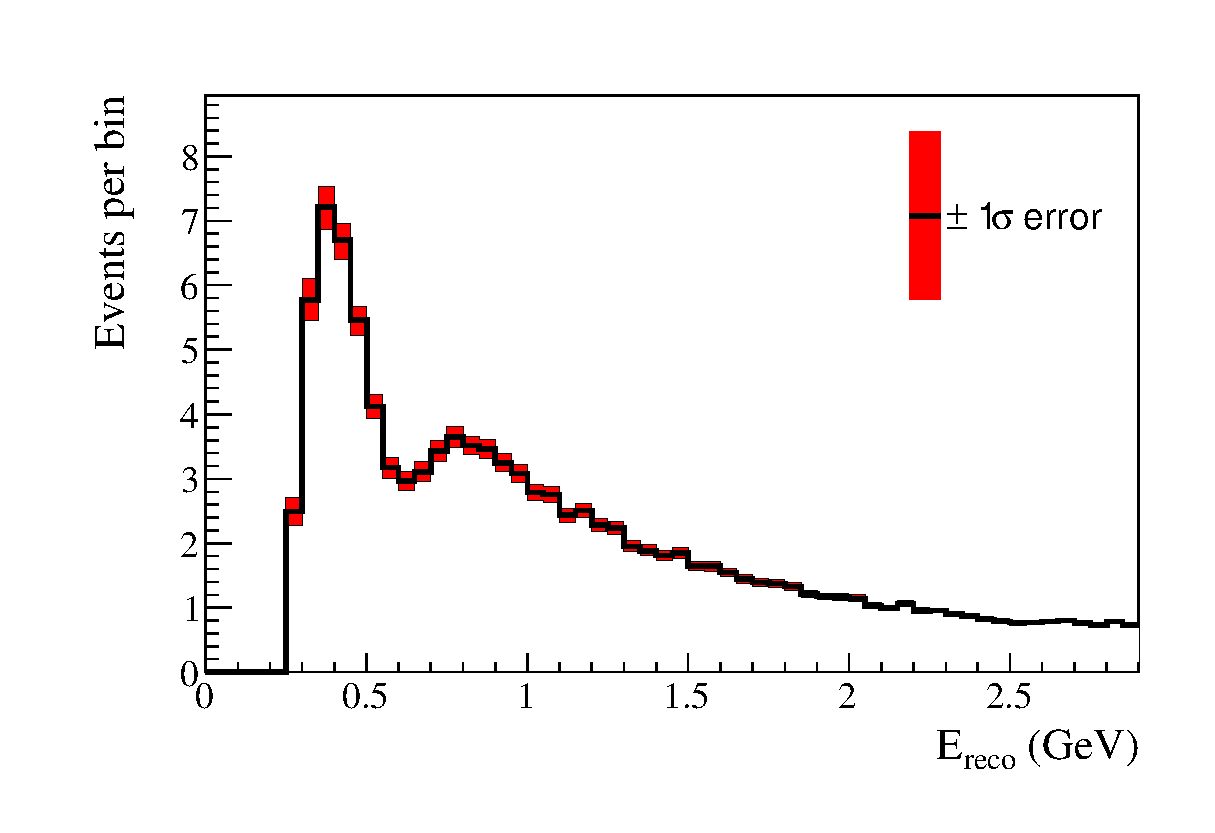
\includegraphics[width=0.9\textwidth]{joint_plots/systematics/Run17c/Asimov_A_1Rmuoscillated_BANFF_xsec_envelope.eps} 
\caption{Muon-like, neutrino mode}
\end{subfigure}
\begin{subfigure}[b]{0.49\textwidth} \centering
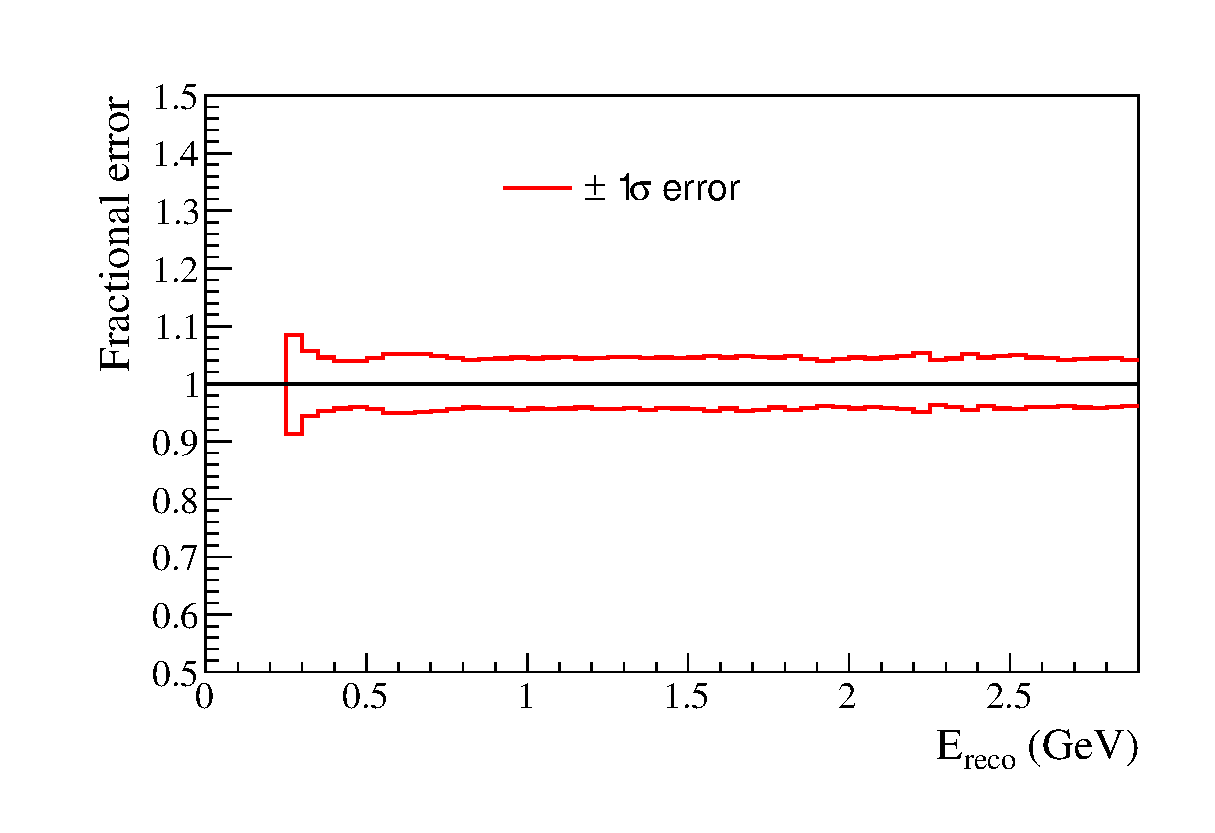
\includegraphics[width=0.9\textwidth]{joint_plots/systematics/Run17c/Asimov_A_1Rmuoscillated_BANFF_xsec_envelope_ratio.eps} 
\caption{Muon-like, neutrino mode}
\end{subfigure}
%rhc mu-like
\begin{subfigure}[b]{0.49\textwidth} \centering
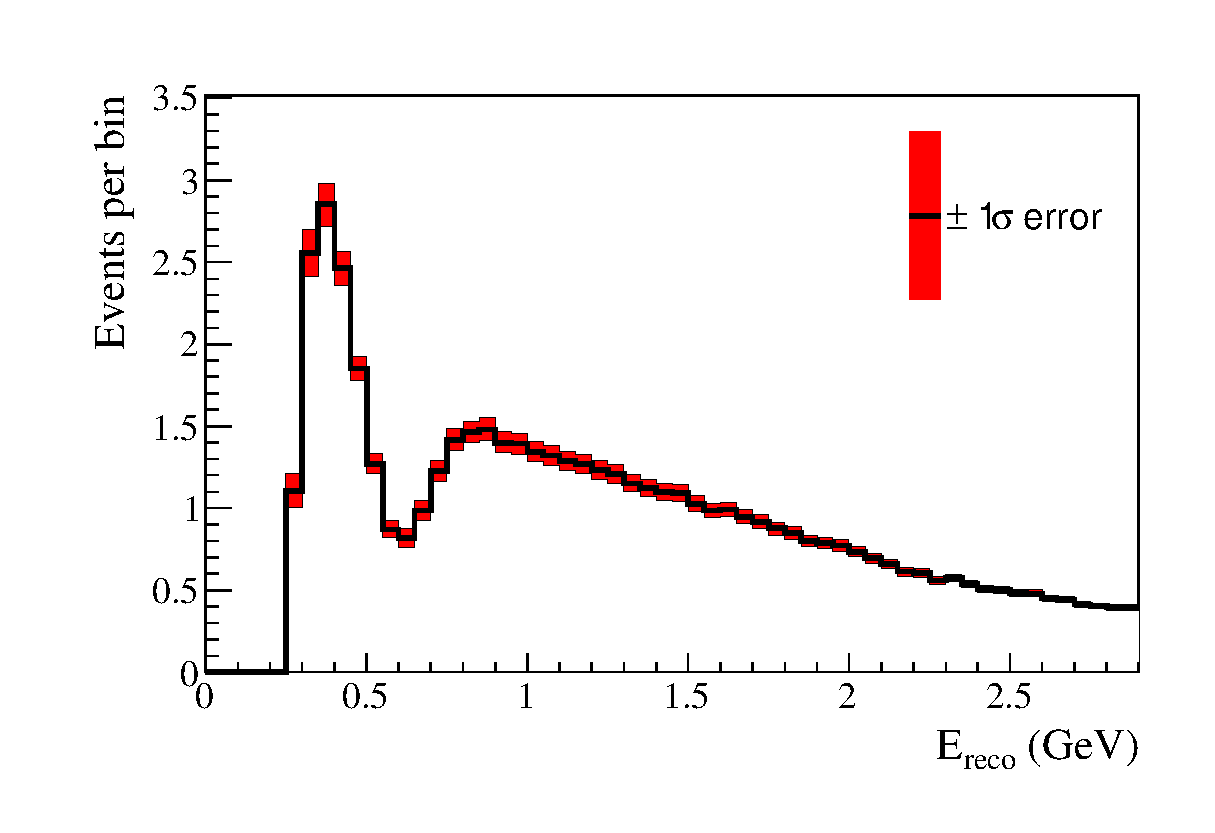
\includegraphics[width=0.9\textwidth]{joint_plots/systematics/Run17c/Asimov_A_RHC1Rmuoscillated_BANFF_xsec_envelope.eps} \\ 
\caption{Muon-like, antineutrino mode}
\end{subfigure}
\begin{subfigure}[b]{0.49\textwidth} \centering
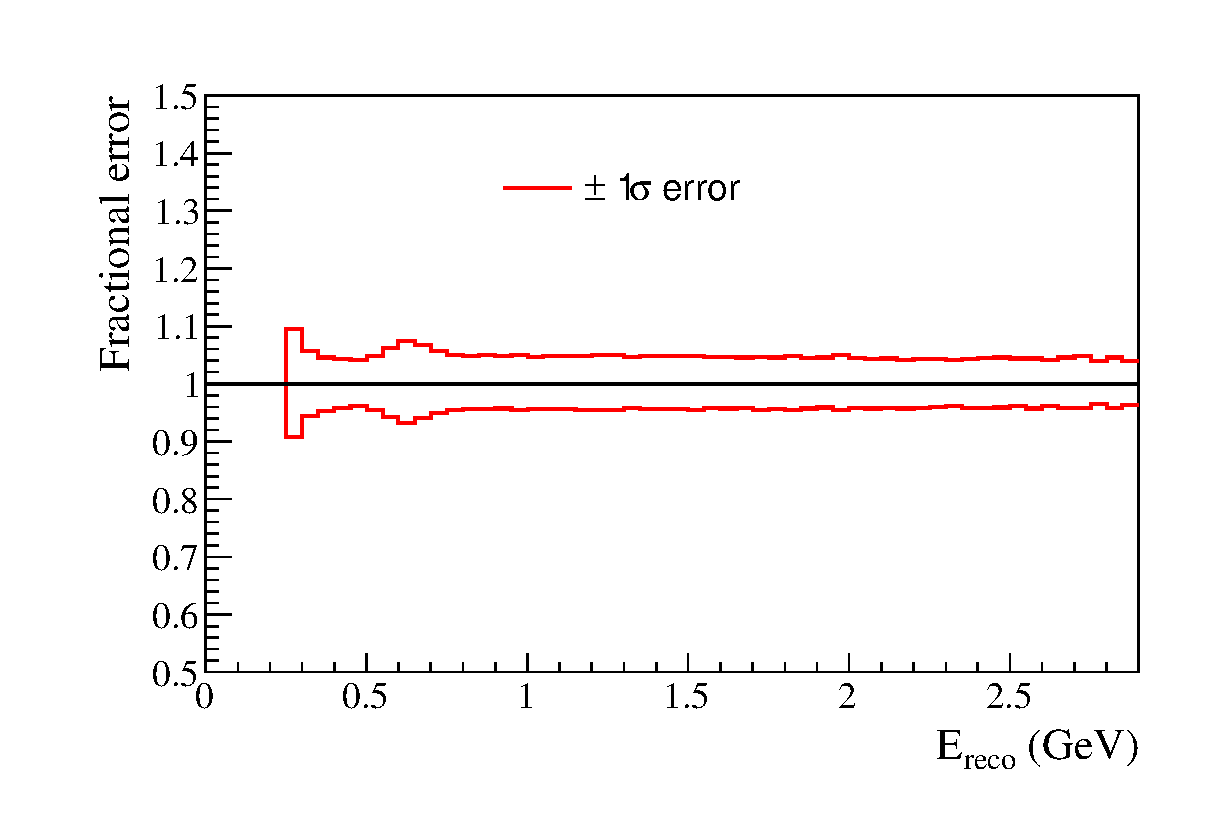
\includegraphics[width=0.9\textwidth]{joint_plots/systematics/Run17c/Asimov_A_RHC1Rmuoscillated_BANFF_xsec_envelope_ratio.eps} \\ 
\caption{Muon-like, antineutrino mode}
\end{subfigure}
%fhc e-like
\caption {
Error envelopes (left) and fractional errors (right) for the reconstructed neutrino energy spectrum
as a result of the cross section systematic parameters. 
	10k toy MC experiments are generated for the Asimov data set A shown in \cref{tab:osc_params_joint_asimov}
	with random systematic parameters, taking into account their correlations.
	Since the parameters $\delta_{CP}$, $\theta_{23}$ and $\Delta m^2_{32}$ ($\Delta m^2_{13}$) and mass hierarchy
will be measured,
only the uncertainty on 
$\sin^2 \theta_{13}$,
$\sin^2 \theta_{12}$
and 
$\Delta m^2_{21}$ 
are taken into account.
BANFF tuned MC templates are used. 
The distributions correspond to the collected statistics in the full Run 1-7c data set.
The changes due to the Run 1-7c flux and covariance matrix updates are applied.
}
\label{fig:xsec_envelope_Asimov_A_run17c_mulike}
\end{figure*}


\begin{figure*}[htb]
\center

\begin{subfigure}[b]{0.49\textwidth} \centering
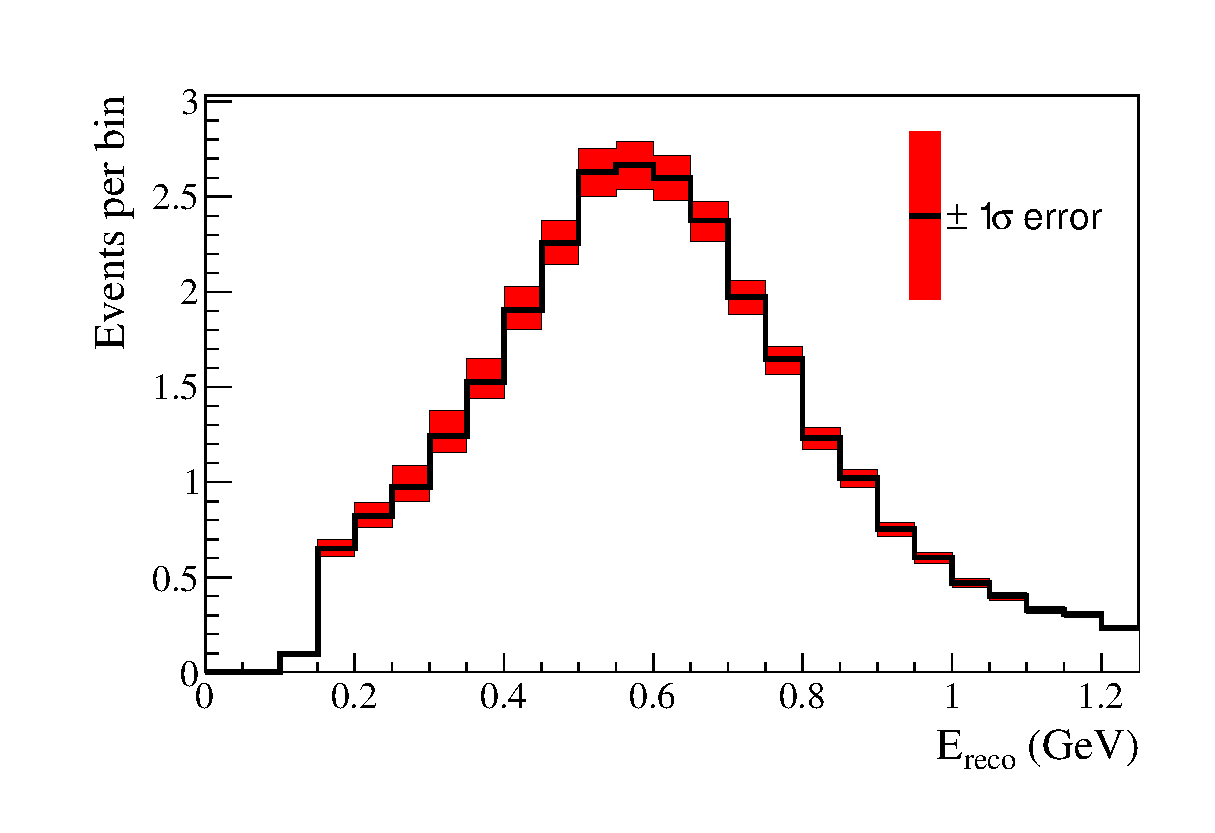
\includegraphics[width=0.9\textwidth]{joint_plots/systematics/Run17c/Asimov_A_1Reoscillated_BANFF_xsec_envelope.eps} 
\caption{Electron-like, neutrino mode}
\end{subfigure}
\begin{subfigure}[b]{0.49\textwidth} \centering
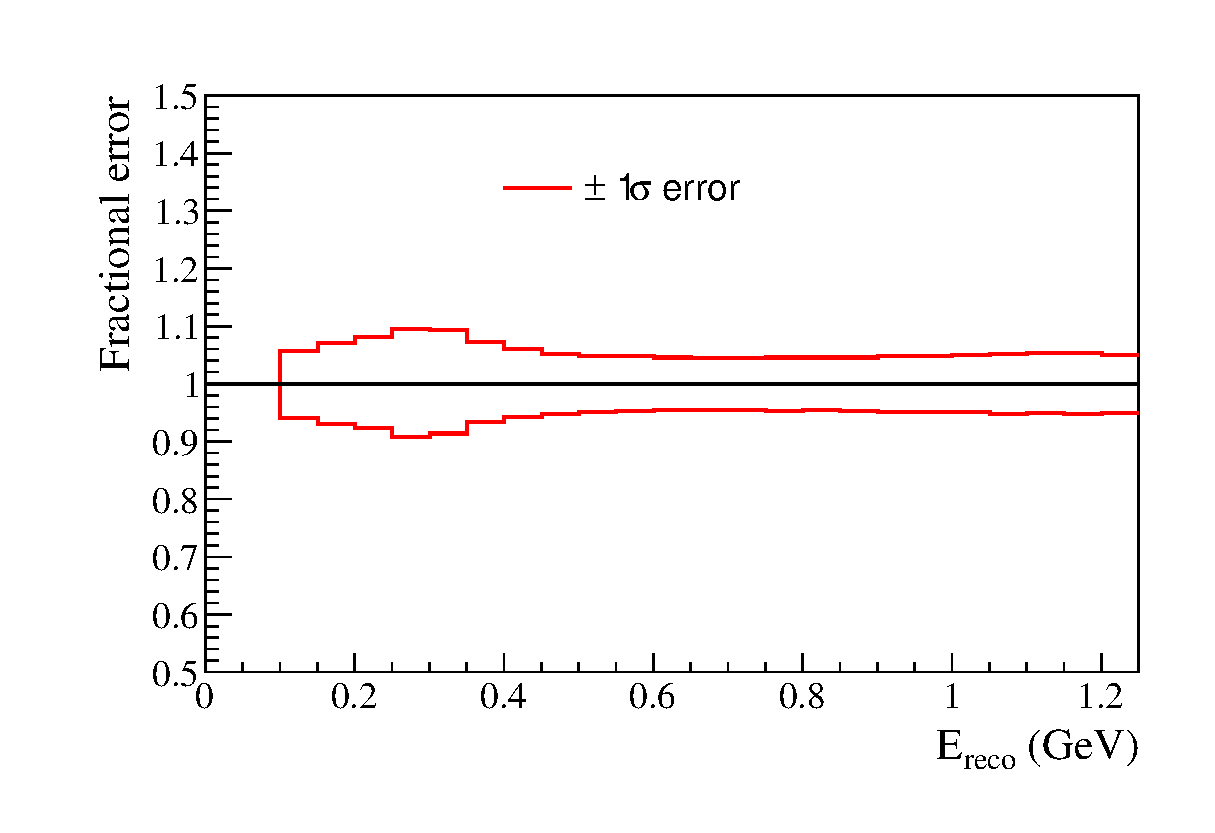
\includegraphics[width=0.9\textwidth]{joint_plots/systematics/Run17c/Asimov_A_1Reoscillated_BANFF_xsec_envelope_ratio.eps} 
\caption{Electron-like, neutrino mode}
\end{subfigure}
%rhc e-like
\begin{subfigure}[b]{0.49\textwidth} \centering
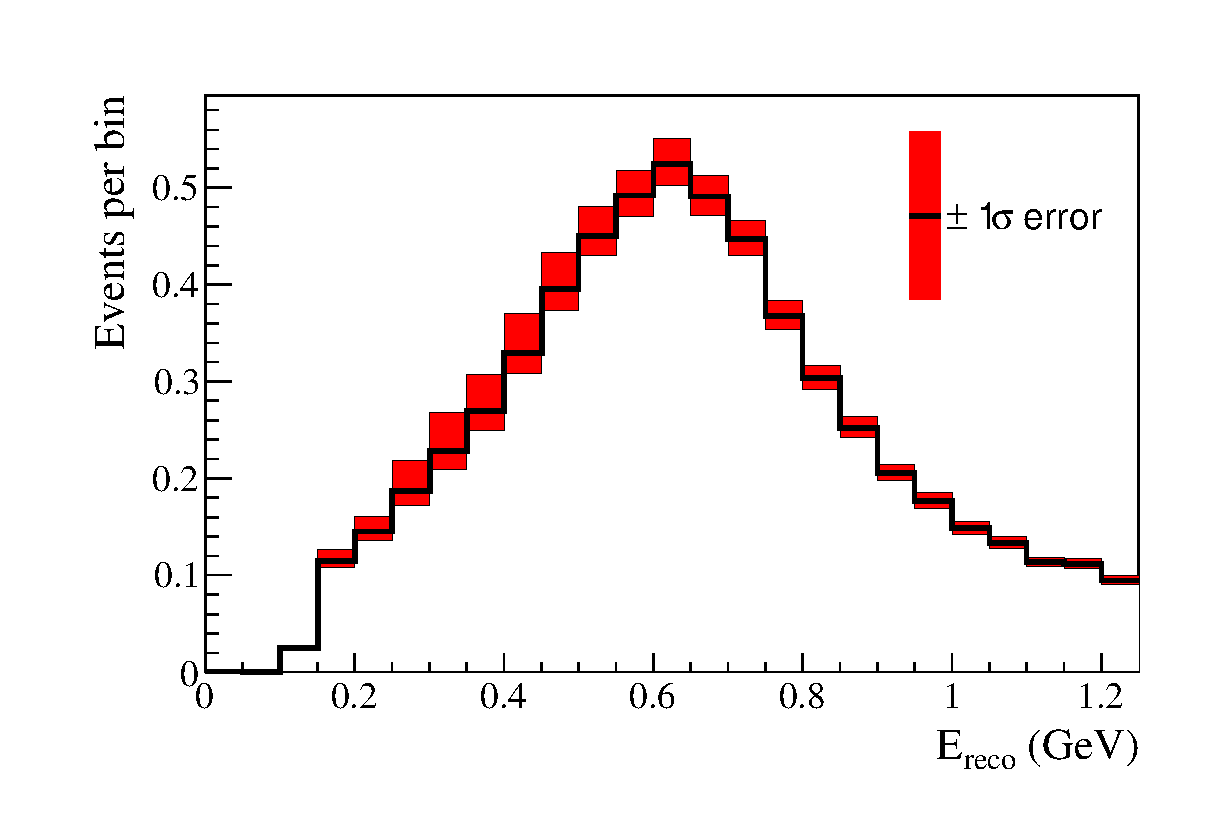
\includegraphics[width=0.9\textwidth]{joint_plots/systematics/Run17c/Asimov_A_RHC1Reoscillated_BANFF_xsec_envelope.eps} 
\caption{Electron-like, antineutrino mode}
\end{subfigure}
\begin{subfigure}[b]{0.49\textwidth} \centering
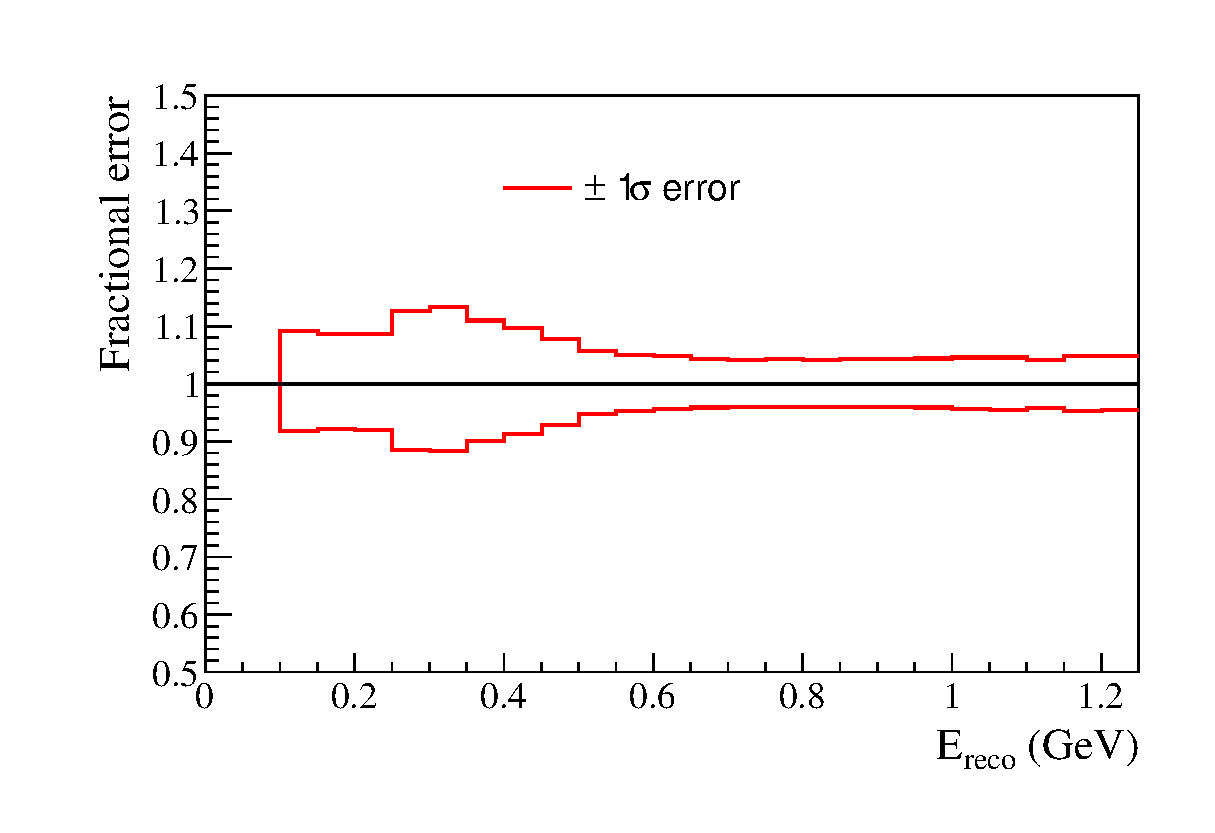
\includegraphics[width=0.9\textwidth]{joint_plots/systematics/Run17c/Asimov_A_RHC1Reoscillated_BANFF_xsec_envelope_ratio.eps} 
\caption{Electron-like, antineutrino mode}
%fhc ccpi-like
\begin{subfigure}[b]{0.49\textwidth} \centering
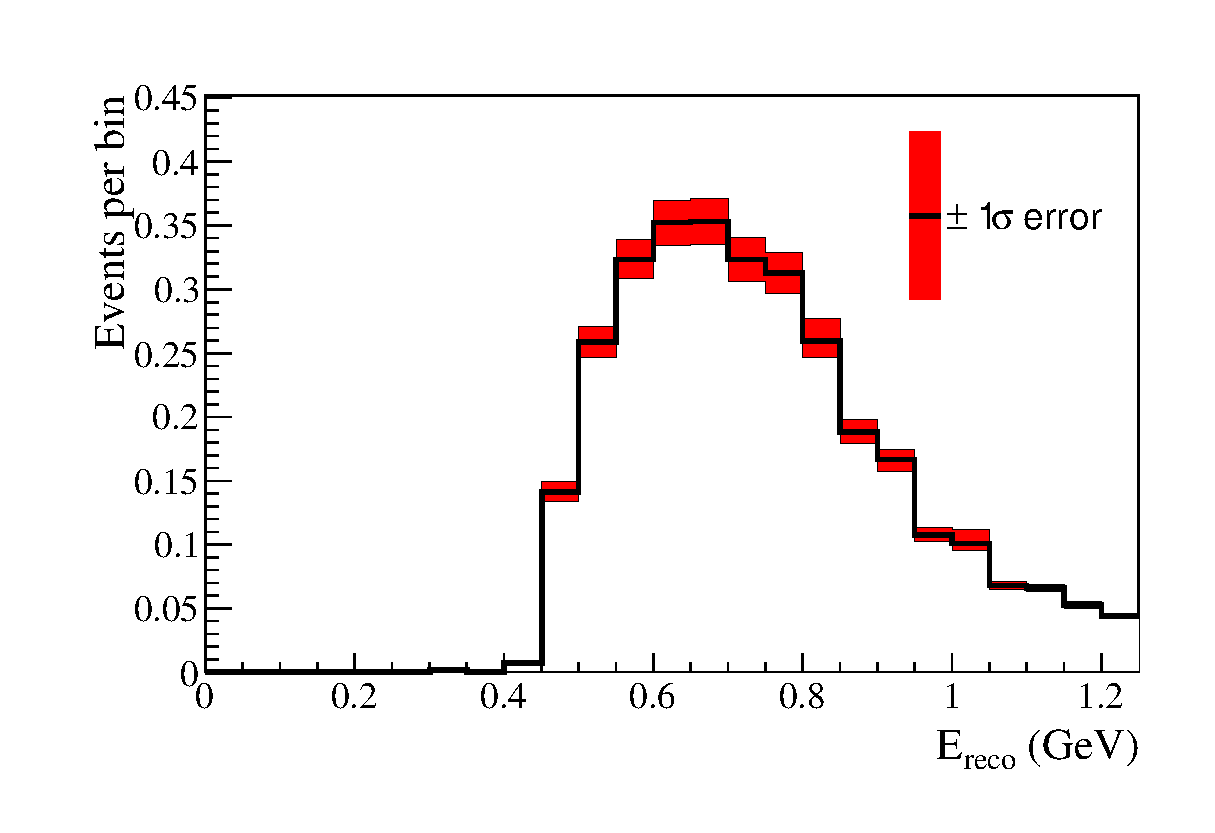
\includegraphics[width=0.9\textwidth]{joint_plots/systematics/Run17c/Asimov_A_MultiReoscillated_BANFF_xsec_envelope.eps} 
\caption{\nueCConepi{}, neutrino mode}
\end{subfigure}
\begin{subfigure}[b]{0.49\textwidth} \centering
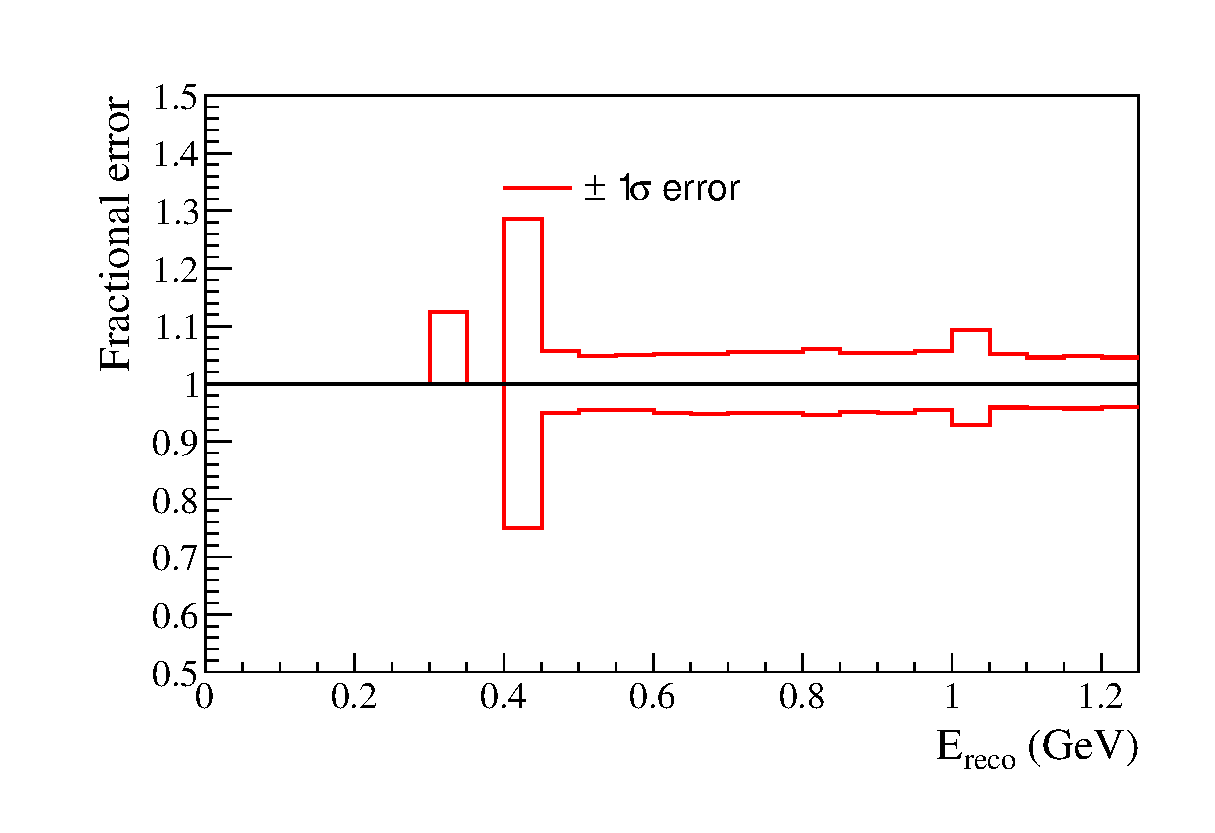
\includegraphics[width=0.9\textwidth]{joint_plots/systematics/Run17c/Asimov_A_MultiReoscillated_BANFF_xsec_envelope_ratio.eps} 
\caption{\nueCConepi{}, neutrino mode}
\end{subfigure}
\end{subfigure}
\caption {
Error envelopes (left) and fractional errors (right) for the reconstructed neutrino energy spectrum
as a result of the cross section systematic parameters. 
10k toy MC experiments are generated for the Asimov data set A shown in \cref{tab:osc_params_joint_asimov}
with randomised systematic parameters, taking into account their correlations.
Since the parameters $\delta_{CP}$, $\theta_{23}$ and $\Delta m^2_{32}$ ($\Delta m^2_{13}$) and mass hierarchy
will be measured,
only the uncertainty on 
$\sin^2 \theta_{13}$,
$\sin^2 \theta_{12}$
and 
$\Delta m^2_{21}$ 
are taken into account.
BANFF tuned MC templates are used. 
The distributions correspond to the collected statistics in the full Run 1-7c data set.
The changes due to the Run 1-7c flux and covariance matrix updates are applied.
}
\label{fig:xsec_envelope_Asimov_A_run17c_elike}
\end{figure*}


\begin{figure*}[htb]
\center
%fhc mu-like
\begin{subfigure}[b]{0.49\textwidth} \centering
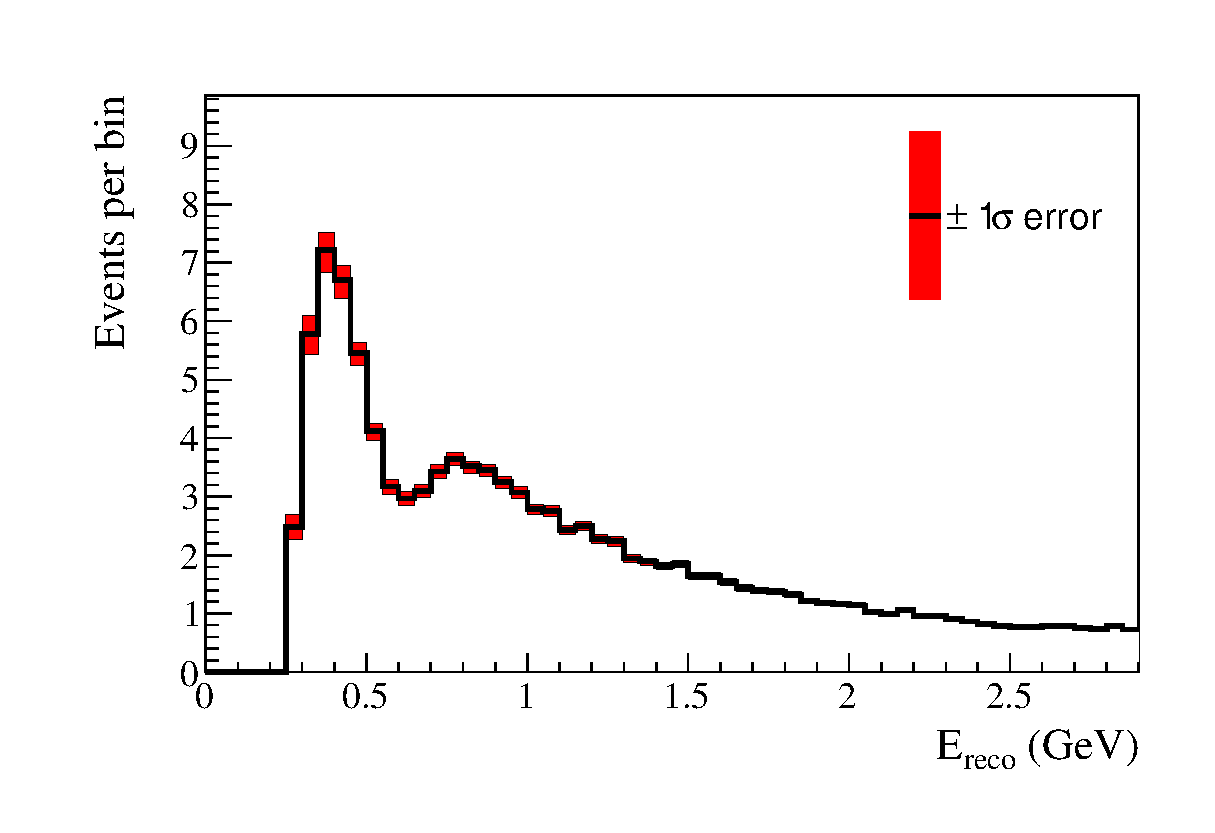
\includegraphics[width=0.9\textwidth]{joint_plots/systematics/Run17c/Asimov_A_1Rmuoscillated_BANFF_envelope.eps} 
\caption{Muon-like, neutrino mode}
\end{subfigure}
\begin{subfigure}[b]{0.49\textwidth} \centering
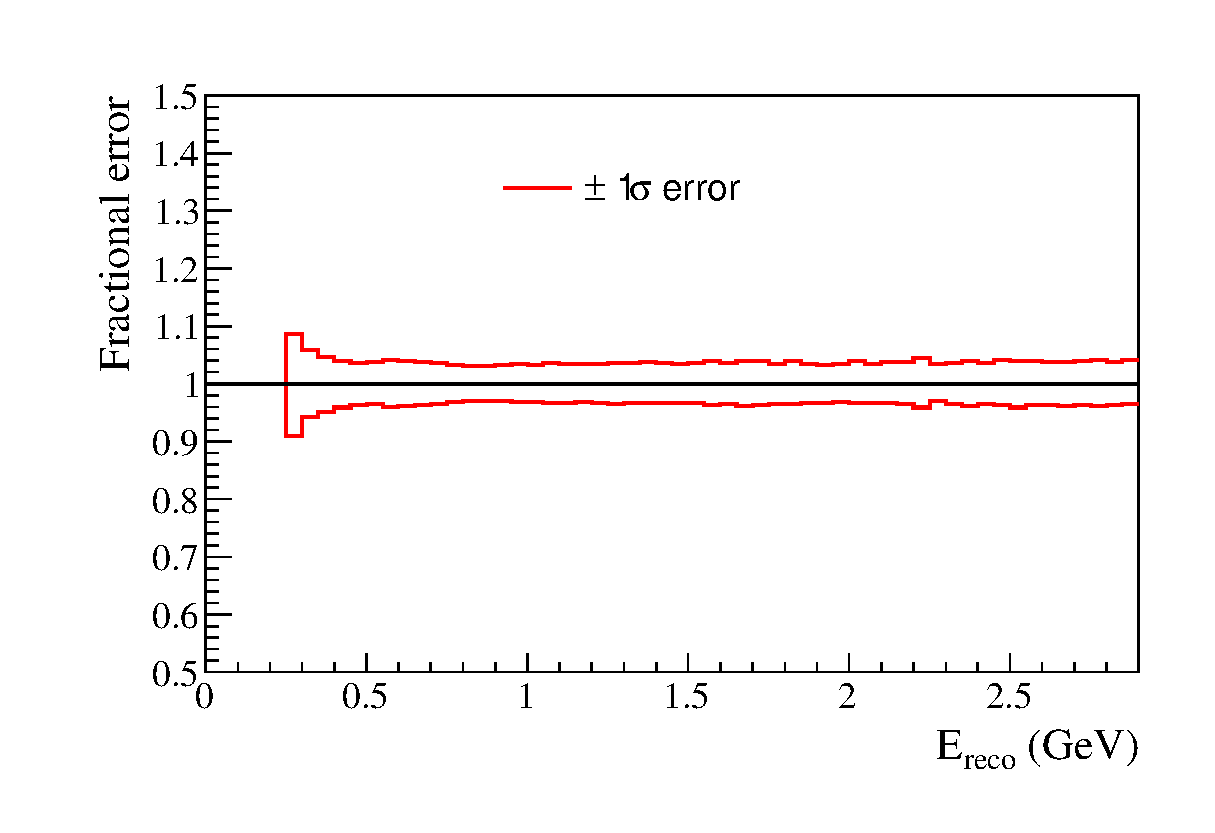
\includegraphics[width=0.9\textwidth]{joint_plots/systematics/Run17c/Asimov_A_1Rmuoscillated_BANFF_envelope_ratio.eps} 
\caption{Muon-like, neutrino mode}
\end{subfigure}
%fhc mu-like
\begin{subfigure}[b]{0.49\textwidth} \centering
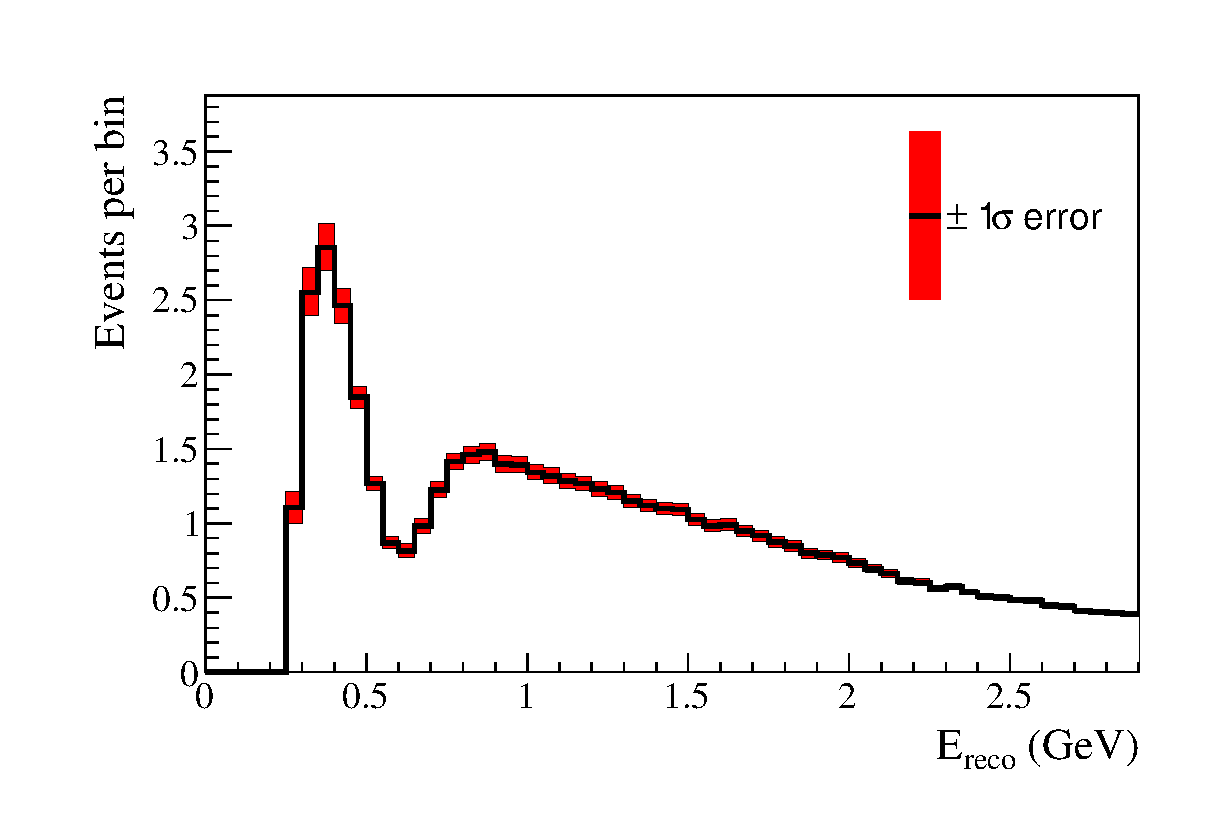
\includegraphics[width=0.9\textwidth]{joint_plots/systematics/Run17c/Asimov_A_RHC1Rmuoscillated_BANFF_envelope.eps} \\ 
\caption{Muon-like, antineutrino mode}
\end{subfigure}
\begin{subfigure}[b]{0.49\textwidth} \centering
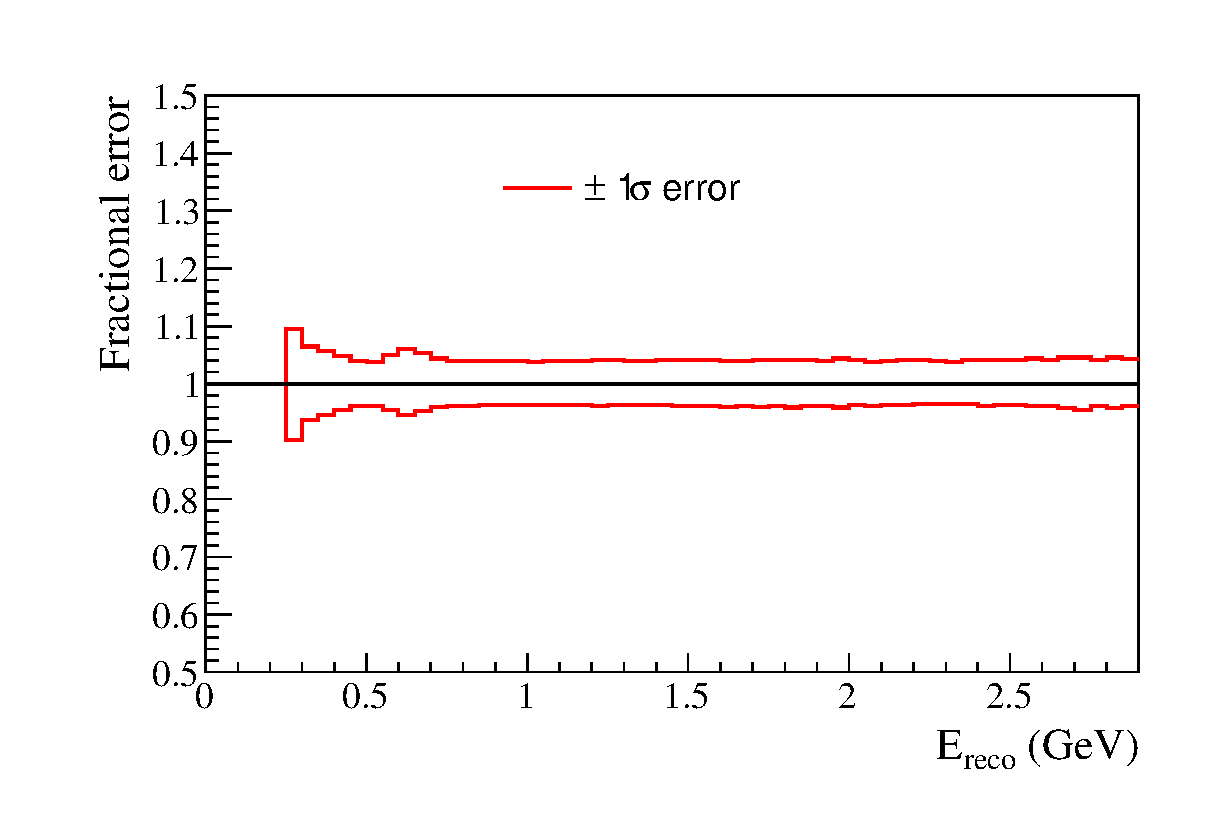
\includegraphics[width=0.9\textwidth]{joint_plots/systematics/Run17c/Asimov_A_RHC1Rmuoscillated_BANFF_envelope_ratio.eps} \\ 
\caption{Muon-like, antineutrino mode}
\end{subfigure}
%fhc mu-like
\caption {
Error envelopes (left) and fractional errors (right) for the reconstructed neutrino energy spectrum
as a result of the flux plus cross section systematic parameters. 
	10k toy MC experiments are generated for the Asimov data set A shown in \cref{tab:osc_params_joint_asimov}
	with random systematic parameters, taking into account their correlations.
	Since the parameters $\delta_{CP}$, $\theta_{23}$ and $\Delta m^2_{32}$ ($\Delta m^2_{13}$) and mass hierarchy
will be measured,
only the uncertainty on 
$\sin^2 \theta_{13}$,
$\sin^2 \theta_{12}$
and 
$\Delta m^2_{21}$ 
are taken into account.
BANFF tuned MC templates are used. 
The distributions correspond to the collected statistics in the full Run 1-7c data set.
The changes due to the Run 1-7c flux and covariance matrix updates are applied.
}
\label{fig:flux_xsec_envelope_Asimov_A_run17c_mulike}
\end{figure*}


\begin{figure*}[htb]
\center

\begin{subfigure}[b]{0.49\textwidth} \centering
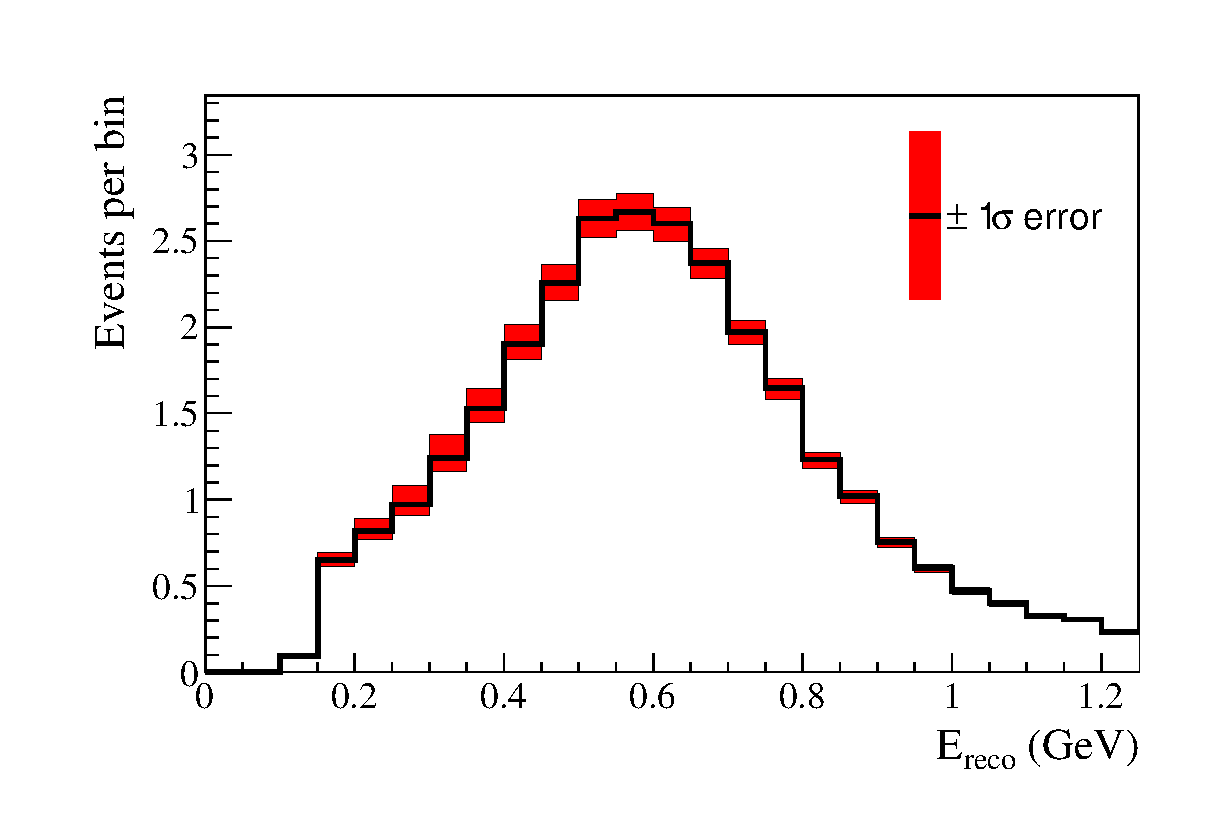
\includegraphics[width=0.9\textwidth]{joint_plots/systematics/Run17c/Asimov_A_1Reoscillated_BANFF_envelope.eps} 
\caption{Electron-like, neutrino mode}
\end{subfigure}
\begin{subfigure}[b]{0.49\textwidth} \centering
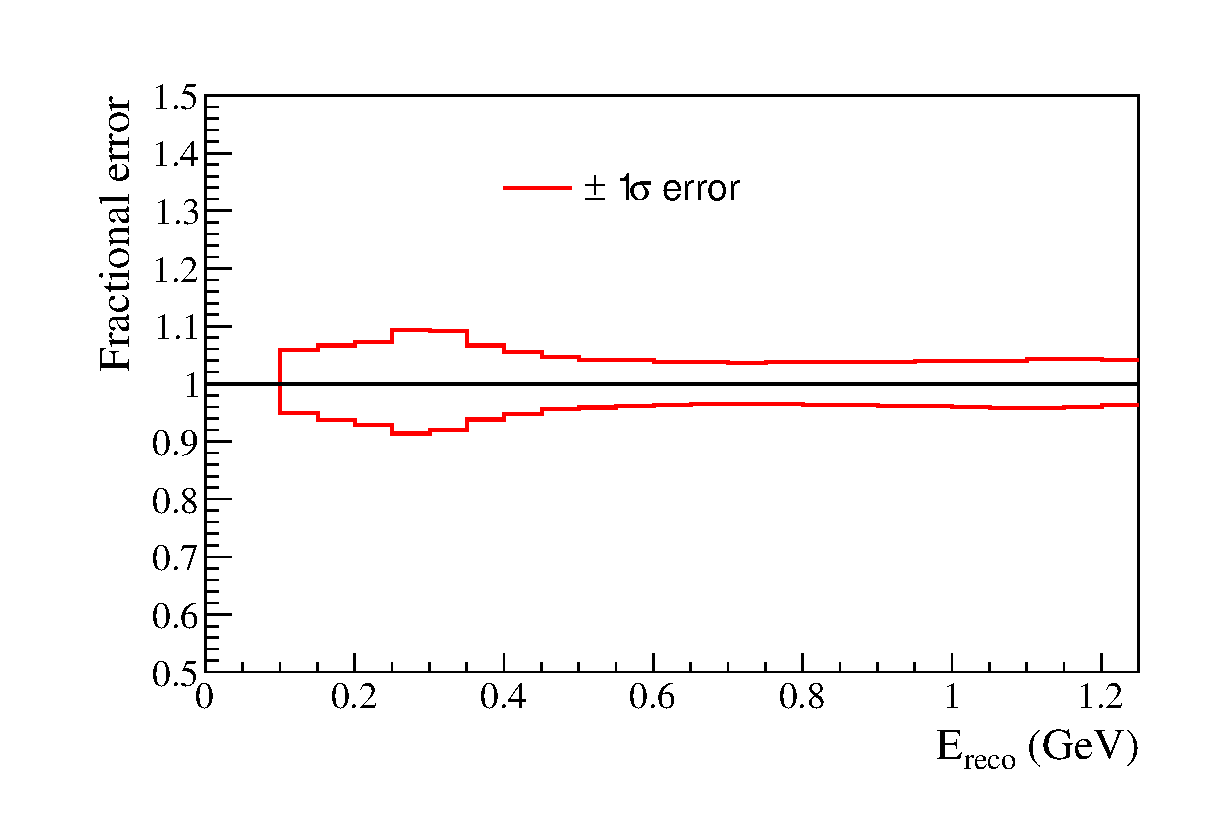
\includegraphics[width=0.9\textwidth]{joint_plots/systematics/Run17c/Asimov_A_1Reoscillated_BANFF_envelope_ratio.eps} 
\caption{Electron-like, neutrino mode}
\end{subfigure}
%fhc mu-like
\begin{subfigure}[b]{0.49\textwidth} \centering
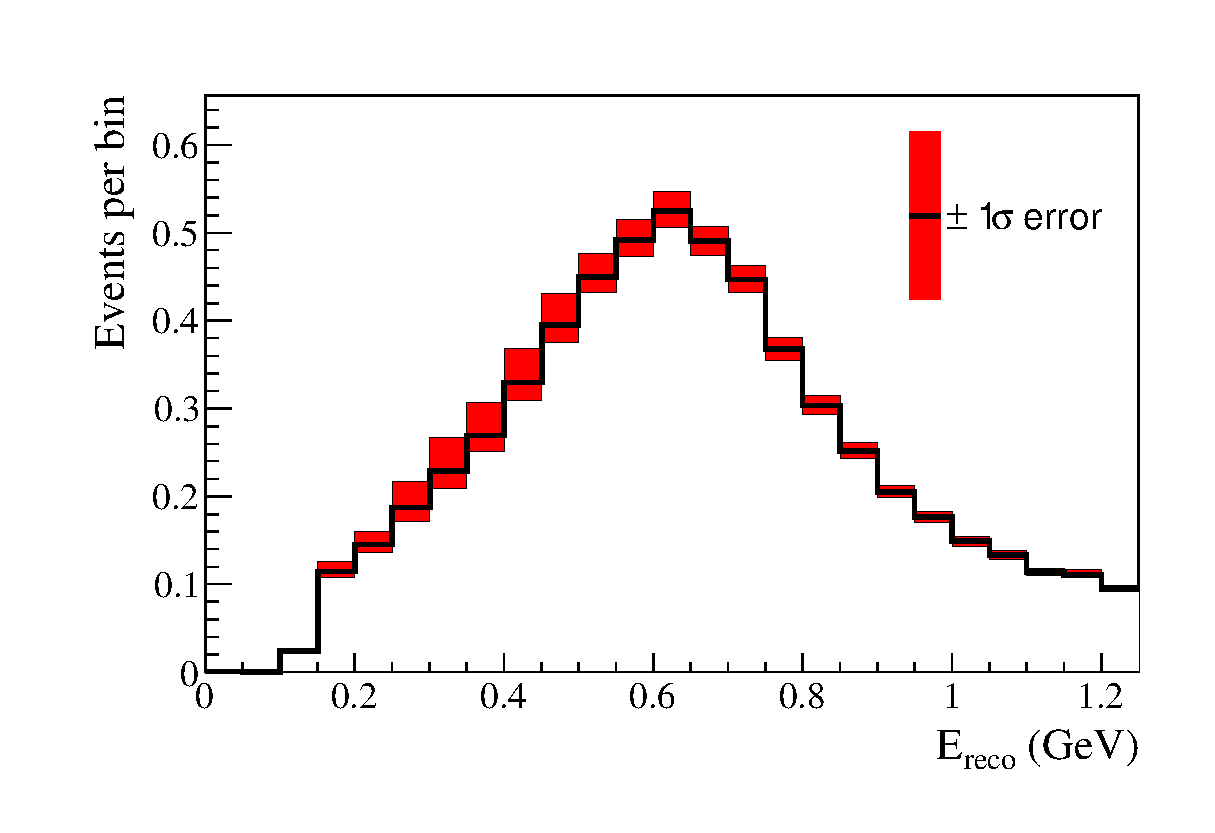
\includegraphics[width=0.9\textwidth]{joint_plots/systematics/Run17c/Asimov_A_RHC1Reoscillated_BANFF_envelope.eps} 
\caption{Electron-like, antineutrino mode}
\end{subfigure}
\begin{subfigure}[b]{0.49\textwidth} \centering
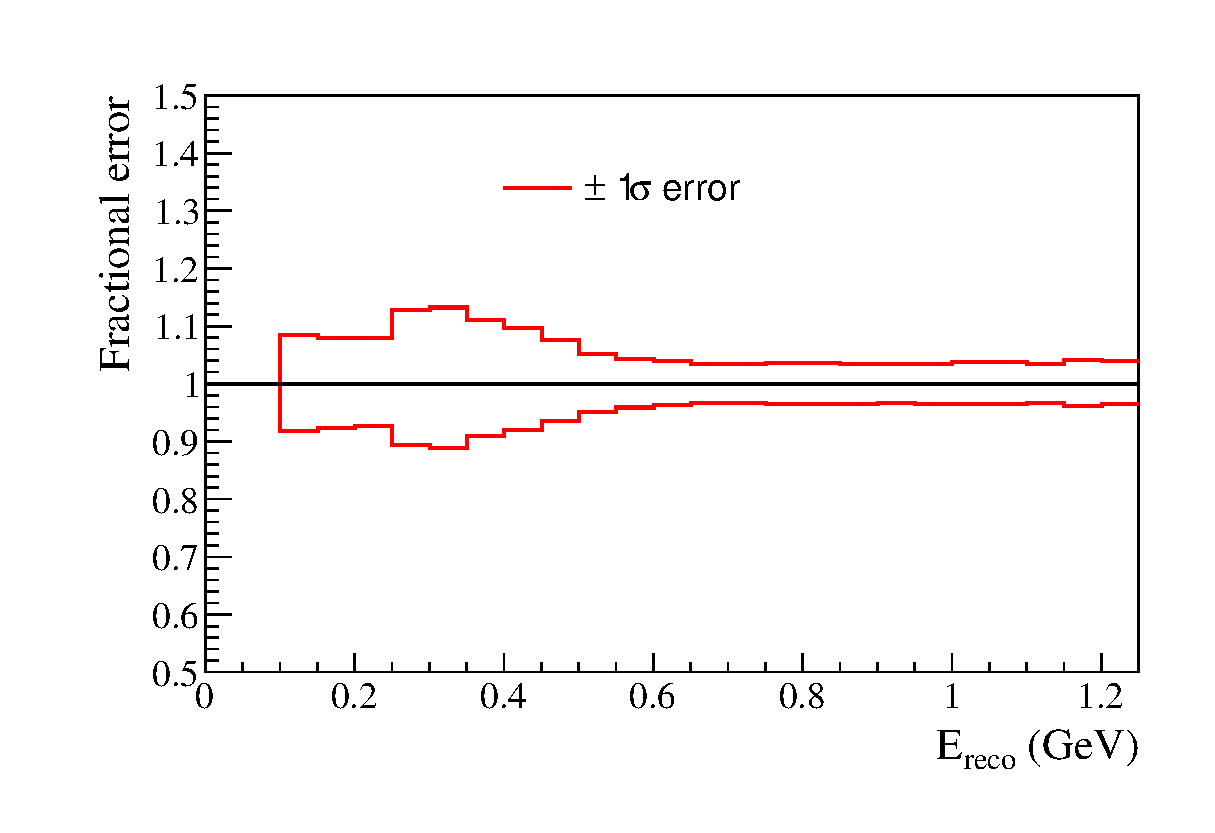
\includegraphics[width=0.9\textwidth]{joint_plots/systematics/Run17c/Asimov_A_RHC1Reoscillated_BANFF_envelope_ratio.eps} 
\caption{Electron-like, antineutrino mode}
\end{subfigure}
%fhc mu-like
\begin{subfigure}[b]{0.49\textwidth} \centering
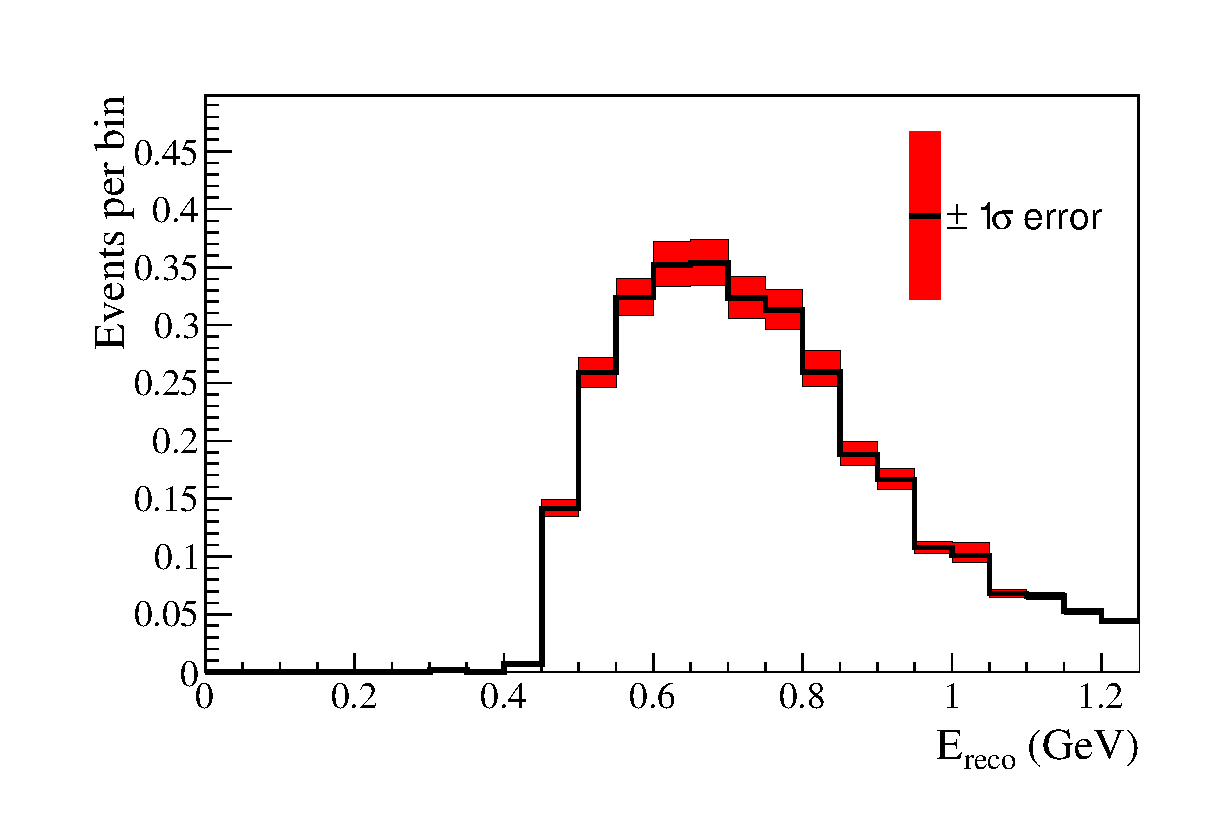
\includegraphics[width=0.9\textwidth]{joint_plots/systematics/Run17c/Asimov_A_MultiReoscillated_BANFF_envelope.eps} 
\caption{\nueCConepi{}, neutrino mode}
\end{subfigure}
\begin{subfigure}[b]{0.49\textwidth} \centering
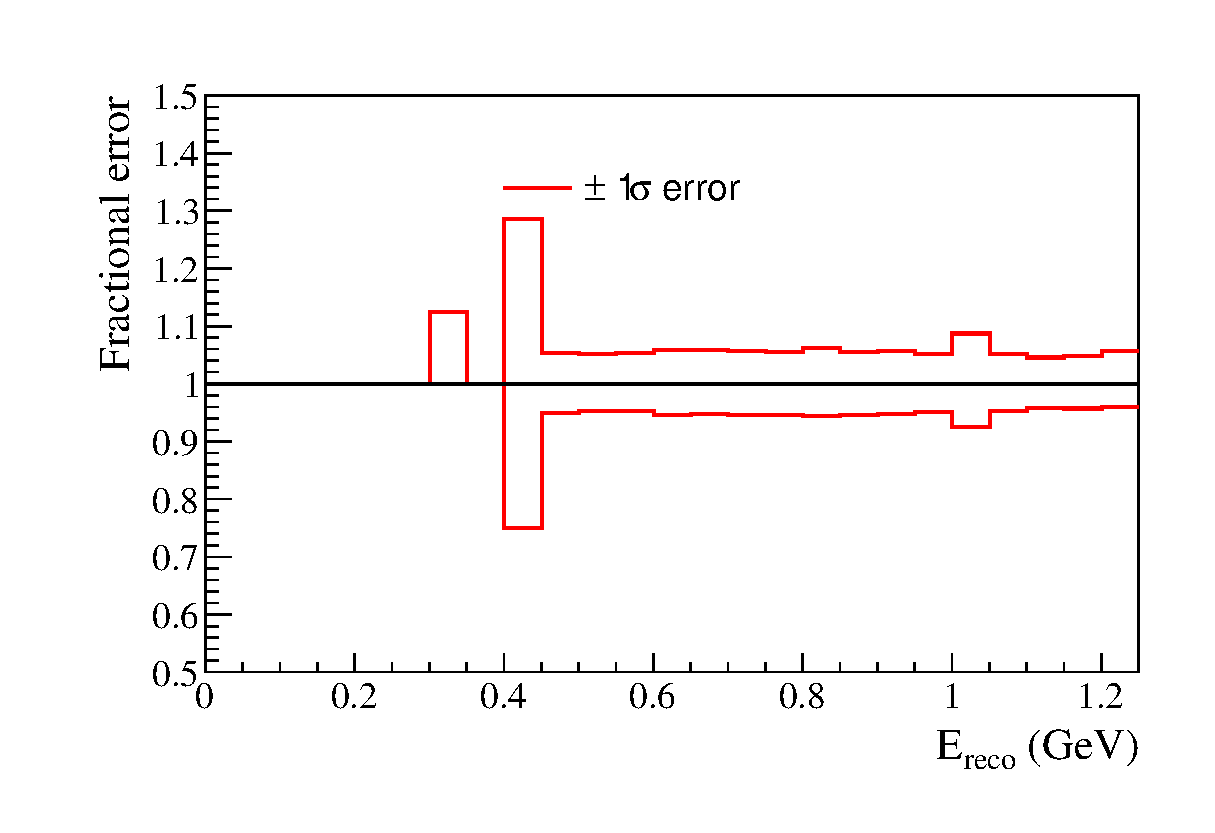
\includegraphics[width=0.9\textwidth]{joint_plots/systematics/Run17c/Asimov_A_MultiReoscillated_BANFF_envelope_ratio.eps} 
\caption{\nueCConepi{}, neutrino mode}
\end{subfigure}
\caption {
Error envelopes (left) and fractional errors (right) for the reconstructed neutrino energy spectrum
as a result of the flux plus cross section systematic parameters. 
10k toy MC experiments are generated for the Asimov data set A shown in \cref{tab:osc_params_joint_asimov}
with randomised systematic parameters, taking into account their correlations.
Since the parameters $\delta_{CP}$, $\theta_{23}$ and $\Delta m^2_{32}$ ($\Delta m^2_{13}$) and mass hierarchy
will be measured,
only the uncertainty on 
$\sin^2 \theta_{13}$,
$\sin^2 \theta_{12}$
and 
$\Delta m^2_{21}$ 
are taken into account.
BANFF tuned MC templates are used. 
The distributions correspond to the collected statistics in the full Run 1-7c data set.
The changes due to the Run 1-7c flux and covariance matrix updates are applied.
}
\label{fig:flux_xsec_envelope_Asimov_A_run17c_elike}
\end{figure*}




\clearpage














%%
%% Posterior predictive method
%%
%
%\subsection{Posterior predictive method for the choice of the prior}
%\label{sec:posterior_predictive_run17c}
%
%The posterior predictive method has been tested for the Run 1-7c statistic as well
%using the same procedure described in \cref{sec:posterior_predictive}.
%
%As shown in \cref{tab:critval_posterior_Asimov_A_run17c} and~\ref{tab:critval_posterior_Asimov_B_run17c}
%the posterior predictive critical values obtained for Asimov data sets A and B
%at $1\sigma$, 90\% and $2\sigma$ CL are similar to the prior predictive ones,
%as for the previous analyses. 
%
%\begin{figure*}[htb]
%\center
%%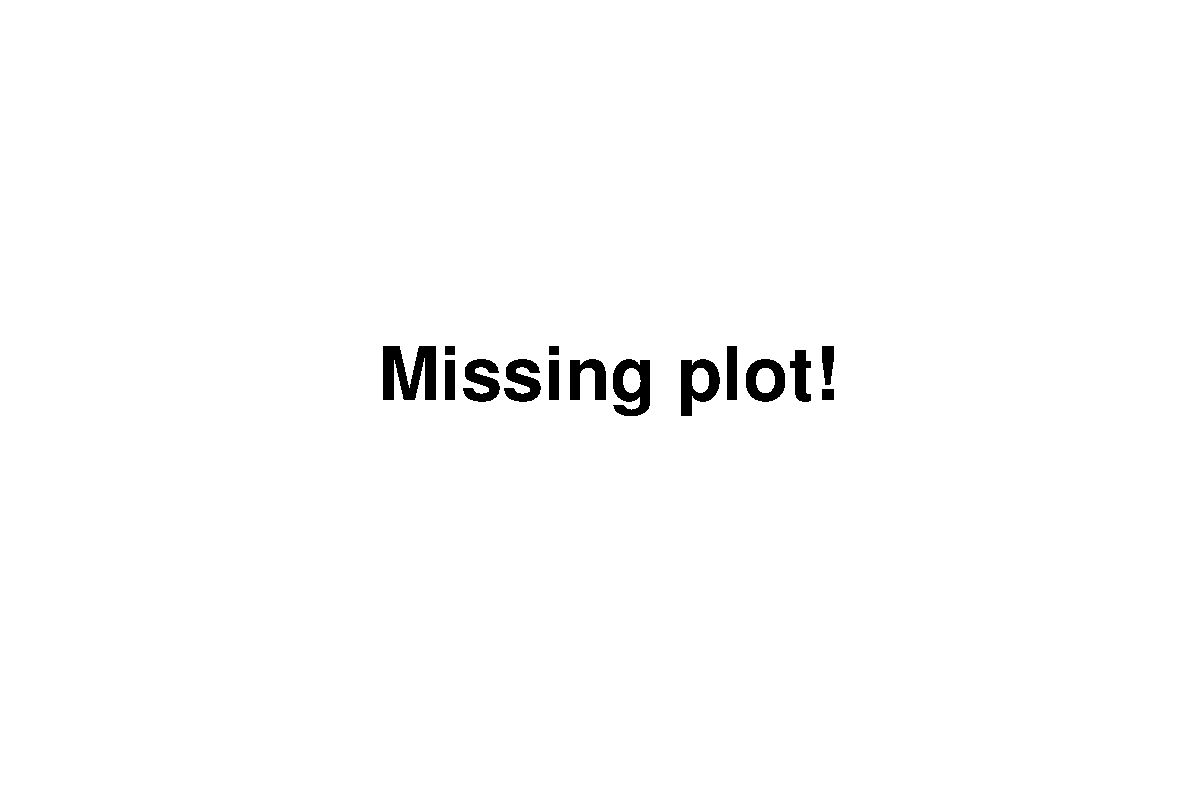
\includegraphics[width=0.9\textwidth]{./images/missing_plot-eps-converted-to.pdf}
%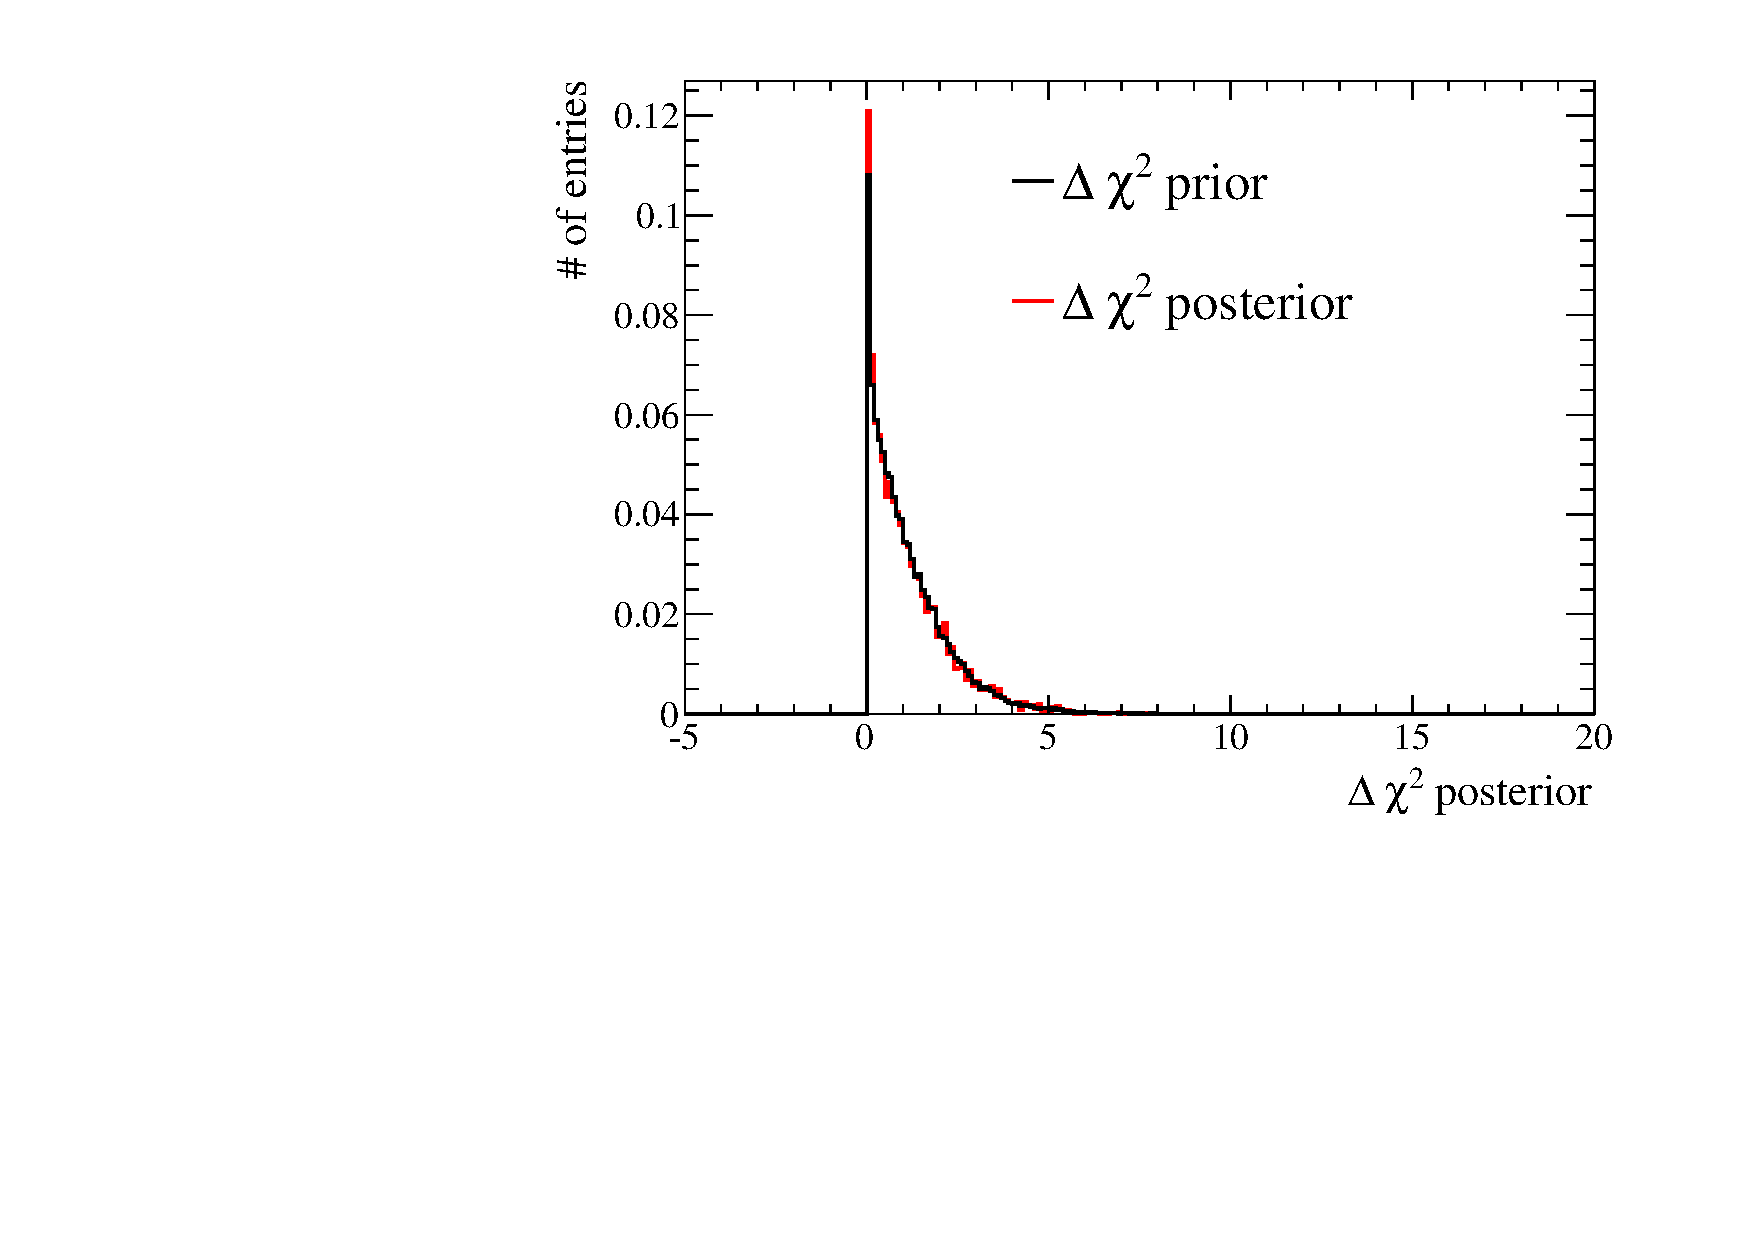
\includegraphics[width=0.49\textwidth]{./joint_plots/coverage_fc/posterior_predictive_run17c/Asimov_A/deltachisq_posterior_Asimov_A.pdf}
%\caption {
%$\Delta \chi^2$ distributions with prior (black) and posterior (red) predictive methods.
%The comparison between the two distributions normalized to 1 is shown.
%Fake data sets are generated with $\delta_{CP} = 0$ and normal hierarchy.
%The Asimov data A is used to generate the weights of the fake data sets.
%50k fake data sets are used.
%Since the posterior predictive distribution is weighted, the effective number of entries is lower with respect 
%to the prior predictive case. 
%}
%\label{fig:post_Asimov_A_dcp_0_nh_run17c}
%\end{figure*}
%
%
%\begin{table}
%\center
%\begin{tabular}{| c | c | c |}
%\hline
%{\bf CL} 				& {\bf Prior} &{\bf Posterior}  \\
%\hline
%\hline
%\multicolumn{3}{| c | }{$\delta^{true}_{CP} = 0$, $MH^{true} = \text{normal}$}  \\
%\hline
%$1\sigma$				&1.390  		& $1.360 ^{+0.024}_{-0.024}$	\\ \hline	
%90\%					&2.592  		& $2.583 ^{+0.053}_{-0.058}$	\\ \hline	
%$2\sigma$				&3.391 		& $3.413 ^{+0.078}_{-0.049}$	\\ \hline	
%\hline
%\multicolumn{3}{| c | }{$\delta^{true}_{CP} = 0$, $MH^{true} = \text{inverted}$}  \\
%\hline
%$1\sigma$				&1.356  		& $1.365 ^{+0.019}_{-0.025}$	\\ \hline	
%90\%					&2.618  		& $2.660 ^{+0.058}_{-0.040}$	\\ \hline	
%$2\sigma$				&3.430 		& $3.411 ^{+0.088}_{-0.040}$	\\ \hline	
%\hline
%\multicolumn{3}{| c | }{$\delta^{true}_{CP} = -1.351$, $MH^{true} = \text{inverted}$}  \\
%\hline
%$1\sigma$				&1.180   		& $ 1.171^{+0.021}_{-0.017}$	\\ \hline	
%90\%					&2.362		& $ 2.249^{+0.036}_{-0.042}$	\\ \hline	
%$2\sigma$				&3.306 		& $ 3.100^{+0.067}_{-0.084}$	\\ \hline	
%\end{tabular}
%\caption{
%The critical values of $\Delta \chi^2$ computed with Feldman-Cousins
%for both prior and posterior predictive method are shown.
%50k toy experiments were used. 
%%for 
%%$\delta_{CP} = 0$ and normal hierarchy
%%and
%%about 50k toy experiments were used for 
%%$\delta_{CP} = 0$ and inverted hierarchy
%%and
%%$\delta_{CP} = -1.351$ and inverted hierarchy,
%The weights of the fake data sets were generated with the Asimov data set A.
%}             
%\label{tab:critval_posterior_Asimov_A_run17c}                                                                                                                                                                             
%\end{table}
%
%
%\begin{table}
%\center
%\begin{tabular}{| c | c | c |}
%\hline
%{\bf CL} 				& {\bf Prior} &{\bf Posterior}  \\
%\hline
%\hline
%\multicolumn{3}{| c | }{$\delta^{true}_{CP} = 0$, $MH^{true} = \text{normal}$}  \\
%\hline
%$1\sigma$				& 1.390 		& $1.325 ^{+0.024}_{-0.023}$	\\ \hline	
%90\%					& 2.592 		& $2.601 ^{+0.041}_{-0.039}$	\\ \hline	
%$2\sigma$				& 3.391		& $3.448 ^{+0.045}_{-0.047}$	\\ \hline	
%\hline
%\multicolumn{3}{| c | }{$\delta^{true}_{CP} = 0$, $MH^{true} = \text{inverted}$}  \\
%\hline
%$1\sigma$				&1.356  		& $1.340 ^{+0.020}_{-0.021}$	\\ \hline	
%90\%					&2.618  		& $2.574 ^{+0.037}_{-0.032}$	\\ \hline	
%$2\sigma$				&3.430  		& $3.310 ^{+0.039}_{-0.045}$	\\ \hline	
%\hline
%\multicolumn{3}{| c | }{$\delta^{true}_{CP} = -1.351$, $MH^{true} = \text{inverted}$}  \\
%\hline
%$1\sigma$				&1.180  		& $ 1.196^{+0.014}_{-0.022}$	\\ \hline	
%90\%					& 2.362 		& $2.383 ^{+0.037}_{-0.042}$	\\ \hline	
%$2\sigma$				& 3.306		& $3.399 ^{+0.0681}_{-0.102}$	\\ \hline	
%\end{tabular}
%\caption{
%The critical values of $\Delta \chi^2$ computed with Feldman-Cousins
%for both prior and posterior predictive method are shown.
%50k toy experiments were used. 
%%for
%%$\delta_{CP} = 0$ and normal hierarchy
%%and
%%about 50k toy experiments were used for 
%%$\delta_{CP} = 0$ and inverted hierarchy
%%and
%%$\delta_{CP} = -1.351$ and inverted hierarchy,
%The weights of the fake data sets were generated with the Asimov data set B.
%}             
%\label{tab:critval_posterior_Asimov_B_run17c}                                                                                                                                                                             
%\end{table}


\clearpage




%
% Validation minimization algorithm
%




\clearpage

\section {Analysis procedure}
\label{sec:oscfit}

%--------------------------------------------------------------------------------------------------------------------
\subsection {Fit method}
\label{sec:oscfit_method}

The goal of this analysis is to measure the oscillation parameters
$\sin^2 \theta_{13}$, $\sin^2 \theta_{23}$, $\Delta m^2_{32}$ and
search for CP violation by setting limits on $\delta_{CP}$
for a given hypothesis of mass hierarchy, which is fixed to either normal or inverted.
All the systematics, as well as the oscillation parameters which are not measured
in that particular analysis and treated as nuisance, are marginalised.
The treatment of the oscillation parameters is shown in \cref{tab:osc_params_joint_priors}.
The parameters of interest will be denoted with the vector $\vec{\theta}$,
since more than 1 parameter at a time can be measured.
$\vec{\theta}$ can include the combination of all the oscillation parameters listed above.

%--------------------------------------------------------------------------------------------------------------------

The {\em VALOR} analysis uses a binned likelihood-ratio method where
the estimation of $\vec{\theta}$ is obtained
by comparing the observed and predicted Super-K $E_{reco}$ vs $\theta_l$ spectra
for 1-ring events.

Let $N$ be the number of reconstructed energy and lepton angle bins and
${\bf a}$ be a $1 \times N_{s}$ - dimensional array of systematic (nuisance) 
parameters that affect the Super-K reconstructed energy spectrum prediction (e.g.
parameters that control the beam, neutrino interaction simulations, 
detector response and oscillations).


The log-likelihood function used in the analysis is

\begin{equation} \label{eq:chisquare}
%\displaystyle
%\chi^{2} 
-2 \; \textrm{ln} \; \lambda (\vec{\theta},{\bf a}) = 2 \cdot \sum_{i=0}^{N-1} 
   \Big( 
     n^{obs}_{i} \cdot \textrm{ln} (n^{obs}_{i}/n^{exp}_{i}) +
     (n^{exp}_{i}-n^{obs}_{i}) 
   \Big) 
\end{equation}
where
$n^{obs}_{i}$ is the observed number of events in the $i^{th}$ bin and
$n^{exp}_{i} = n^{exp}_{i}(\vec{\theta}; {\bf a})$ 
%$n^{exp}_{i} = n^{exp}_{i}(\sin^{2}\overline{\theta}_{23},|\overline{\Delta m}^{2}_{32}|; {\bf a})$ 
is the corresponding expected number of events.


The log-likelihood function obtained by adding a gaussian penatly term can be written as
\begin{equation} \label{eq:chisquare_penalty}
%\displaystyle
%\chi^{2} 
-2 \; \textrm{ln} \; \lambda (\vec{\theta},{\bf a}) = 2 \cdot \sum_{i=0}^{N-1} 
   \Big( 
     n^{obs}_{i} \cdot \textrm{ln} (n^{obs}_{i}/n^{exp}_{i}) +
     (n^{exp}_{i}-n^{obs}_{i}) 
   \Big) +
   ({\bf a}-{\bf a_{0}})^{T} \cdot {\bf C}^{-1} \cdot ({\bf a}-{\bf a_{0}})
\end{equation}
where
${\bf a_{0}}$ is an $1 \times N_{s}$ - dimensional array with the default values of 
the systematic parameters, ${\bf a}^{T}$ is the transpose of ${\bf a}$,
${\bf C}$ is the systematic parameter covariance matrix of dimension $N_{s} \times N_{s}$,
$n^{obs}_{i}$ is the observed number of events in the $i^{th}$ bin, and
$n^{exp}_{i}(\vec{\theta}; {\bf a})$ 
%$n^{exp}_{i} = n^{exp}_{i}(\sin^{2}\overline{\theta}_{23},|\overline{\Delta m}^{2}_{32}|; {\bf a})$ 
is the corresponding expected number of events.

The total likelihood is given by the product of the likelihood terms of each selected sample,

\begin{equation} \label{eq:totlike}
\lambda(\vec{\theta}; {\bf a}) = \prod_{s=1}^{N_{samples}} \lambda_s (\vec{\theta}; {\bf a})
\end{equation}
where $N_{samples}$ is the number of selected samples used in the analysis, or
by the sum of $-2 \; \textrm{ln} \; \lambda (\vec{\theta},{\bf a})$ from all the Super-K samples

\begin{equation} \label{eq:totlike_2}
-2 \; \textrm{ln} \; \lambda (\vec{\theta},{\bf a}) = \sum_{s=1}^{N_{samples}} -2 \; \textrm{ln} \; \lambda_s (\vec{\theta},{\bf a})
\end{equation}

The advantage of the used binned likelihood ratio method is that,
in the large-sample limit, the quantity 
$-2 \: \textrm{ln} \: \lambda (\vec{\theta}; {\bf a})$
%$-2 \: \textrm{ln} \: \lambda (\sin^{2}\overline{\theta}_{23},|\overline{\Delta m}^{2}_{32}|; {\bf a})$
in \cref{eq:chisquare} has a $\chi^{2}$ distribution and it can therefore be used as a goodness-of-fit test.

Values of systematic parameters that give a negative predicted number of events in any reconstructed energy bin in any interaction 
mode are not allowed. If a systematic throw gives a negative number of events, that toy experiment is rejected.

%--------------------------------------------------------------------------------------------------------------------                                                                                    

\subsection {Marginalization}
\label{sec:marginalization}

In the previous analyses,
except \cite{OurRun56AntiNueBarAppearanceAnalysis3Flavour},
 a fully frequentist approach, in which all nuisance parameters were profiled, was used.
Now a hybrid Bayesian-frequentist method is used. 
The nuisance parameters are marginalised over while the parameters of interest are minimized with respect to the likelihood distribution.
The marginalization of the nuisance parameters give a so-called marginal likelihood that depends on only
on a vector of parameters of interest, $\vec{\theta}$.

The marginal likelihood is derived using the following equation:

\begin{equation}\label{eq:likemarg}
\lambda_{marg} (\vec{\theta}) = \int_{A} \lambda (\vec{\theta};{\bf a}) \pi{({\bf a})} d {\bf a} = \frac{1}{n} \sum_{i=1}^{n} 
\lambda (\vec{\theta}; {\bf a}_i) 
\end{equation}
where ${\bf a}$ is the set of nuisance parameters in the parameter space $A$, $\pi{({\bf a})}$ is the prior of the nuisance parameters.
$n$ is the number of toys MC produced for the marginalization and
${\bf a_i}$ is the single set of nuisance parameters extracted in the ``i-th" toy MC.
Many sets of ${\bf a}$ should be extracted in order to effectively sample the space of the nuisance parameters.
The number of extractions depends on the number of nuisance parameters as well as the precision that is required by the measurement.
In all the analyses shown in this note $n = 10k$ toys MC were used for the marginalisation of the systematic parameters.

We use the marginal log-likelihood, which will be denoted as $\chi^2_{marg}$ from now on,
since it follows a $\chi^2$ distribution when the Poisson statistic converges to the Gaussian:

\begin{equation} \label{eq:loglikemarg}
\chi^2_{marg} (\vec{\theta}) = - 2  \ln \lambda_{marg} (\vec{\theta})  = -2 \ln \left(\frac{1}{n} \sum_{i=1}^{n} 
\lambda (\vec{\theta}; {\bf a}_i)  \right) 
\end{equation}
It is important to note that this numerical integration is a weighted average of the likelihood evaluated at the $n$ throws, 
not a weighted average of the log-likelihood.
%When marginalization is used the penalty term
%$ ({\bf a}-{\bf a_{0}})^{T} \cdot {\bf C}^{-1} \cdot ({\bf a}-{\bf a_{0}}) $
%For this reason a modified version of \cref{eq:chisquare}, which doesn't include the penalty term, is used.
During the marginalization process, random values of the nuisance parameters are drawn according to the prior constraints which come from fits to near detector data and control samples at Super-K. Therefore, each throw is already weighted based on the prior information, and as a result the nuisance parameter values are not included in the calculation of the likelihood.
%
%When marginalization is used the penalty term becomes useless, 
%since the values of the nuisance parameters are already extracted using the prior distributions
%which replace the penalty term
%$ ({\bf a}-{\bf a_{0}})^{T} \cdot {\bf C}^{-1} \cdot ({\bf a}-{\bf a_{0}})$
%that also becomes constant, independent of the parameter of interest.
%
For this reason \cref{eq:chisquare}, which doesn't include the penalty term, is used.

Sometimes the free parameters, which are not marginalised, 
are constrained with a penalty term.
In this case a modified version of \cref{eq:loglikemarg} is used:

\begin{equation} \label{eq:chisqmarg_with_penalty}
\chi^2_{constr} (\vec{\theta}) = \chi^2_{marg}(\vec{\theta}) + (\vec{\theta} - \vec{\theta_0})^T V^{-1} (\vec{\theta} - \vec{\theta_0}) 
\end{equation}
where $\vec{\theta_0}$ is the vector of nominal values of the parameters of interest,
$\vec{\theta}$ is the vector of its fitted values 
and $V$ is the covariance matrix which relates all the free parameters.
If the constrained parameter $\theta_{constr}$ is not correlated with the other parameters of interest,
$V$ is reduced to the uncertainty $\Delta \theta^{constr}$,
and \cref{eq:chisqmarg_with_penalty} becomes

\begin{equation} \label{eq:chisqmarg_with_penalty_uncorr}
\chi^2_{constr} (\vec{\theta}) = \chi^2_{marg}(\vec{\theta}) + \frac{ (\theta^{constr} - \theta^{constr}_0)^2 }{(\Delta \theta^{constr})^2}
\end{equation}
This is the case of $\sin^2 \theta_{13}$ when it is measured, i.e. it is parameter of interest,
but at the same time it is constrained with the measurement of the reactor experiments.
When a penalty term is applied to a parameter of interest it will be specified.

The toys MC used for the marginalization of the nuisance parameters are performed exactly in the same way as 
described in \cref{sec:systematics:inputs}, taking into account the correlations, but without statistical fluctuations.
First $n = 10k$ distributions of $E_{reco}$ vs $\theta_l$ for $e$-like and $E_{reco}$ only for $\mu$-like samples
are produced using the extracted systematic parameters for a given point of the parameter of interest grid $\vec{\theta}$
for $1 \times 10^{20}$ POT so that they may be scaled appropriately when comparing to datasets of differing POT.
%and normalised to $1 \times 10^{20}$ POT, in order to be used for fits at any different number of POT. 
Finally they are stored in output files which can be used for whatever needed fit.
A fit on a single dataset is performed as following:
\begin{itemize}
\item all the $n$ toy MC distributions are read from the files,
\item each distribution is normalised to the number of POT of the data set,
\item for each toy distribution \cref{eq:chisquare} is calculated and $\lambda(\vec{\theta},{\bf a}) = e^{- (-2 \; \textrm{ln} \; \lambda (\vec{\theta},{\bf a})) / 2}$ is obtained,
\item the $\chi^2$ value is finally obtained, using \cref{eq:loglikemarg}, for a given set of parameter values of interest, $\vec{\theta}$.
	If $\vec{\theta}$ is constrained, \cref{eq:chisqmarg_with_penalty_uncorr} is used.
\end{itemize}

This procedure is followed for each point in the $\vec{\theta}$ grid, where the binning 
is so fine that it does not impact on the precision of the measurement.
Finally the best fit is found by looking for the $\vec{\theta}$ grid point 
with the minimum $\chi^2$ value, $\chi^2_{bf}$.
This point corresponds to the best-fit parameters $\vec{\theta}_{bf}$. 
The minimization can be also performed by using a discrete descent gradient algorithm \cite{DescentGradient}
implemented in the VALOR framework that allows the minimum $\chi^2$ 
to be found without the need of calculating the full $\chi^2$ distribution across all grid points.
This method is employed when a large number of fits is required, such as the calculation of critical values
for Feldman-Cousins contours, as it drastically reduces the amount of CPU time required.
%This will be very useful when many fits are done and a lot of CPU time is required.
A validation of the minimization algorithm will be shown in \cref{sec:validation} %are we showing this in the note or should we reference a previous one?
for the analyses where it is used.


%--------------------------------------------------------------------------------------------------------------------                                                                                    

\subsection{Best-fit spectra with marginalization}
\label{sec:spectra_bestfit_method}

When profiling, the best fit spectra are defined by the MC prediction that gives the largest likelihood values.

%If profiling is used the nuisance parameters are fixed to their best-fit values
%and the computation of the best-fit spectra is straightforward.

However, since the nuisance parameters are marginalised, there does not exist a single set 
of parameters
which corresponds to the best fit. Therefore a new method has been developed to 
represent the best fit spectra which is consistent with the oscillation results. 
%However, since the nuisance parameters are marginalised,
%in order to get the best-fit spectra consistent with the oscillation results,
%the nuisance parameters cannot be set to their best-fit values and
%a new method must be developed.

%At the end of the fit the nuisance parameters have an effective value which corresponds
%to the weighted average over all the toys MC where the weights are 
%the likelihood values of each single toy given by \cref{eq:chisquare}.
%This becomes clearer when considering \cref{eq:likemarg}.

The following procedure is used.
From each toy MC $i$, 
used to marginalise the nuisance parameters, 
a different spectrum,
with 
%$N^{j}(\vec{\theta}_{bf}; \bf{a})$ 
$N^{j}(\vec{\theta}_{bf})$ 
number of events in each bin $j$, 
is produced
as well as a likelihood $\lambda (\vec{\theta}_{bf},\bf{a_i}) $ value, 
calculated using \cref{eq:likemarg},
where 
$\vec{\theta}_{bf}$ is the best-fit value of the free parameters vector
and 
$\bf{a_i}$
is the vector of nuisance parameters corresponding to the toy $i$.
The best-fit number of events in the bin $j$ of the spectrum is calculated as

\begin{equation} \label{eq:bestfit_spectrum_marg}
N^j_{marg} = \frac{ \sum_{i=1}^{n} \lambda (\vec{\theta}_{bf}; {\bf a_i}) \cdot N^{j}(\vec{\theta}_{bf}; {\bf a_i}) }{ \sum_{i=1}^{n} \lambda (\vec{\theta}_{bf}; {\bf a_i})  }
\end{equation}
where $n$ is the number of toys MC.

One can easily find a relation between the profiled and marginalised best-fit spectra.
In the limit of infinite number of toys MC, 
i.e. the full nuisance parameters space is scanned,
the likelihood can be written as
\begin{equation} \label{eq:likemarg_bf}
\lambda_{marg} (\vec{\theta}_{bf}) = \frac{1}{n} \sum_{i=1,~i \neq bf}^{n} \left[ \lambda (\vec{\theta}_{bf}; \bf{a_i}) + \lambda_{prof}  \right]
\end{equation}
where 
$\lambda_{prof} =  \lambda (\vec{\theta}_{bf}; \bf{a_{bf}})$ 
is the profiled best-fit likelihood. 
If we denote as
$N^j_{prof} = N_i^{j}(\vec{\theta}_{bf}; \bf{a_{bf}})$  
the number of events in the bin $j$ obtained with profiling,
\cref{eq:bestfit_spectrum_marg} can be written as

\begin{equation} \label{eq:bestfit_spectrum}
N^j_{marg} = \frac{ \sum_{i=1,~i \neq bf}^{n} \lambda (\vec{\theta}_{bf}; \bf{a_i}) \cdot N^{j}(\vec{\theta}_{bf}; \bf{a_i}) + \lambda_{prof} \cdot N^{j}_{prof}  }{ \sum_{i=1}^{n} \lambda (\vec{\theta}_{bf}; \bf{a_i})  }
\end{equation}
%In the gaussian regime, 
%i.e. the likelihood has a linear dependence from the parameters 
%that are also distributed as gaussian,
%marginalization and profiling gives exactly the same result.
%If the term $\sum_{i=1,~i \neq bf}^{n} \lambda (\vec{\theta}_{bf}; \bf{a_i}) \cdot N^{j}(\vec{\theta}_{bf}; \bf{a_i})$
%is symmetric around $\mathcal{L}_{prof} \cdot N^{j}_{prof}$,
%the marginalised spectrum converges to the one obtained using the profiling and
%$N^j_{marg} = N^{j}_{prof}$.






%--------------------------------------------------------------------------------------------------------------------                                                                                    

\subsection{Confidence intervals}
\label{sec:cl}

After the fit is completed, 
the full $\chi^2$ distribution is then shifted with respect to $\chi^2 (\vec{\theta}_{bf})$:
\begin{equation} \label{eq:deltachisq}
\Delta \chi^2 (\vec{\theta}) = \chi^2(\vec{\theta}) - \chi^2(\vec{\theta}_{bf})
\end{equation}
Confidence intervals are set on $\Delta \chi^2 (\vec{\theta})$.
If 

\begin{equation} \label{eq:condition_cl}
\Delta \chi^2(\vec{\theta}) > \Delta \chi^2_{crit}
\end{equation}
where $\Delta \chi^2_{crit}$ 
is the critical value for a certain confidence level $X\%$(CL),
that value of $\vec{\theta}$ is excluded at the $X\%$ CL.
In the gaussian approximation constant values of $\Delta \chi^2_{crit}$ can be used.
It will be called ``constant $\Delta \chi^2$ method".

However in some cases the gaussian approximation is not reliable
and the ``Feldman-Cousins method" \cite{FeldmanCousins} must be used.
In this method a different critical value for each point of the $\vec{\theta}$ grid 
%$\Delta \chi^2 (\theta_{i..j})_{crit}$
$\Delta \chi^2 (\vec{\theta})_{crit}$
is calculated.
The procedure consists of the following steps:

\begin{enumerate}

\item many toys MC (e.g. 10k) are produced 
	assuming the oscillation hypothesis of the grid point $\vec{\theta}$
 	and taking into account both the statistical and systematic uncertainties; 

\item for each toy first $\chi^2(\vec{\theta}_{fix})$ is obtained
	by minimizing $\chi^2 (\vec{\theta})$
	where the oscillation parameters $\vec{\theta}$ are kept 
	fixed to the values corresponding to the grid point  
	and the nuisance parameters are marginalised.
	Then $\chi^2 (\vec{\theta})$ is minimized, 
	leaving the oscillation parameters $\vec{\theta}$ as free and
	$\chi^2 (\vec{\theta}_{bf})$ is obtained. 
	
\item the test statistic is calculated as

	\begin{equation}
	\Delta \chi^2 = \chi^2(\vec{\theta}_{fix}) - \chi^2 (\vec{\theta}_{bf})
	\end{equation}
	
%\item $\Delta \chi^2 (\vec{\theta})$ is calculated using 
%	\cref{eq:loglikemarg} or~\ref{eq:chisqmarg_with_penalty_uncorr}.

\item The steps 2 and 3 are repeated for each toy MC 
	and $f(\Delta \chi^2)$, the distribution of $\Delta \chi^2 (\vec{\theta})$,
	%analogue to what is shown in fig.~\ref{fig:sterile_pvalue},	
	is obtained.

\item Several critical values for $X\%$ CL (e.g. 68\%, 90\%...),
	%$\Delta \chi^2 (\vec{\theta})_{crit}^{X\%CL}$,
 	$\Delta \chi^2 (\vec{\theta})_{crit}$,
	can be defined as:
	
	\begin{equation} \label{eq:def_crit_val}
	\Delta \chi^2_{crit}: \int_{-\infty}^{\Delta \chi^2_{crit}} f(\Delta \chi^2) d( \Delta \chi^2) = X\%
	\end{equation}		
	
	where $f(\Delta \chi^2)$ is the p.d.f. of $\Delta \chi^2$ and 
	$d( \Delta \chi^2)$ is the differential of the integral.
	
\item This procedure is repeated for all the points of the $\vec{\theta}$ grid
	and several critical values are computed
	
\end{enumerate}

Once a critical value, $\Delta \chi^2 (\vec{\theta})_{crit}$,
is computed for each oscillation hypothesis in the $\vec{\theta}$ grid,
the confidence intervals are set by the condition of \cref{eq:condition_cl}. \\


Several analyses are performed and confidence intervals are computed for:
\begin{itemize}

\item 
1D $\delta_{CP}$ with reactor constraint: 
the parameter of interest is $\delta_{CP}$ and
all the other oscillation parameters are marginalised;
for $\sin^2 \theta_{13}$, that is marginalised,
the gaussian prior of reactor measurements shown in \cref{tab:osc_params_joint_priors}, is used. 

\item 
1D $\delta_{CP}$ T2K only: 
the parameter of interest is $\delta_{CP}$ and
all the other oscillation parameters are marginalised;
for $\sin^2 \theta_{13}$, that is marginalised, 
the uniform prior, shown in \cref{tab:osc_params_joint_priors}, is used. 

\item 
1D $\sin^2 \theta_{13}$ T2K only: 
the parameter of interest is $\sin^2 \theta_{13}$ and
all the other oscillation parameters are marginalised;
%for $\sin^2 \theta_{13}$, that is a free parameter,
%the gaussian prior of reactor measurements shown in \cref{tab:marg_binnning}, is used. 

\item 
1D $\Delta m^2_{32}$ ($\Delta m^2_{13}$) with reactor constraint: 
the parameter of interest is $\Delta m^2_{32}$ ($\Delta m^2_{13}$) and
all the other oscillation parameters are marginalised;
for $\sin^2 \theta_{13}$, that is marginalised,
the gaussian prior of reactor measurements shown in \cref{tab:osc_params_joint_priors}, is used. 

\item 
1D $\sin^2 \theta_{23}$ with reactor constraint: 
the parameter of interest is $\sin^2 \theta_{23}$ and
all the other oscillation parameters are marginalised;
for $\sin^2 \theta_{13}$, that is marginalised,
the gaussian prior of reactor measurements shown in \cref{tab:osc_params_joint_priors}, is used. 

%

\item 
2D $\sin^2 \theta_{13}$ vs $\delta_{CP}$ with reactor constraint: 
the parameters of interest are $\sin^2 \theta_{13}$ and $\delta_{CP}$ while
all the other oscillation parameters are marginalised;
for $\sin^2 \theta_{13}$, that is a free parameter, 
the gaussian prior of reactor measurements shown in \cref{tab:osc_params_joint_priors}, 
is used, through a penalty term as in \cref{eq:chisqmarg_with_penalty_uncorr}.

\item 
2D $\sin^2 \theta_{13}$ vs $\delta_{CP}$ T2K only: 
the parameters of interest are $\sin^2 \theta_{13}$ and $\delta_{CP}$ while
all the other oscillation parameters are marginalised;
%for $\sin^2 \theta_{13}$, that is a free parameter, 
%the uniform prior, shown in \cref{tab:marg_binnning}, is used. 

\item 
2D $\sin^2 \theta_{23}$ vs $\delta_{CP}$ T2K only: 
the parameters of interest are $\sin^2 \theta_{23}$ and $\delta_{CP}$ while
all the other oscillation parameters are marginalised;
%for $\sin^2 \theta_{13}$, that is a free parameter, 
%the uniform prior, shown in \cref{tab:marg_binnning}, is used. 

\item 
2D $\Delta m^2_{32}$ ($\Delta m^2_{13}$) vs $\delta_{CP}$ T2K only: 
the parameters of interest are $\Delta m^2_{32}$ and $\delta_{CP}$ while
all the other oscillation parameters are marginalised;
%for $\sin^2 \theta_{13}$, that is a free parameter, 
%the uniform prior, shown in \cref{tab:marg_binnning}, is used. 

\item 
2D $\sin^2 \theta_{23}$ vs $\Delta m^2_{32}$ ($\Delta m^2_{13}$) with reactor constraint: 
the parameters of interest are $\sin^2 \theta_{23}$ and $\Delta m^2_{32}$ ($\Delta m^2_{13}$) 
while all the other oscillation parameters are marginalised;
for $\sin^2 \theta_{13}$, that is marginalised,
the gaussian prior of reactor measurements shown in \cref{tab:osc_params_joint_priors}, is used. 

\end{itemize}

Each confidence interval is calculated for both normal and inverted hierarchy.

The 1D $\chi^2$ confidence intervals with ``constant $\Delta \chi^2$ method" are used to set the $\pm 1 \sigma$ ranges.

Each point of the $\vec{\theta}$ grid corresponds to the center of the histogram bins,
i.e. the $\chi^2$ values are calculated at each histogram bin center. 
The ranges and binnings used for the analyses listed above are shown in \cref{tab:marg_binnning}.
All the 1-dimensional analyses, where the precision on the best-fit point is important 
and must be quoted, are performed with a fine binning.
Since 2-dimensional analyses are performed only to set contours with ``constant $\Delta \chi^2$ method"
and a fit with a very high precision is not needed to find the best-fit point, 
coarser binning are used, without affecting the contour.
Furthermore a very fine 2-dimensional binning would require much more CPU time and storage space.
In the future $\bar{\nu}/\nu$ joint analysis releases when the "Feldman-Cousins method" will be needed 
also for 2-dimensional fits, a finer binning will be used.

\begin{table}[htb]
\centering
\begin{tabular}{| c | c | c | c | c |}
\hline
Parameter 					& Min 			& Max			& Step			& Bins	  	\\
\hline

& \multicolumn{4}{c|}{\bf 1-dimensional fit}  \\
\hline
$\delta_{CP}$ 					& $-\pi$			& $+\pi$			& $\pi / 200$		& 201		\\
$\sin^2 \theta_{13}$ 	(reactors)	 	& 0.015			& 0.036			& 0.021 / 81		& 201 		\\
$\sin^2 \theta_{13}$ 	(T2K only) 	& 0				& 0.113			& 0.113 / 200		& 201 		\\
$\sin^2 \theta_{23}$ 				& 0.3				& 0.7				& 0.4 / 200 		& 201		\\
$|\Delta m^2_{32}|~(\text{eV}^2 / \text{c}^4)$ 			& $2\times10^{-3}$	& $3\times10^{-3}$	& $10^{-3} / 200$	& 201 		\\
\hline

& \multicolumn{4}{c|}{\bf 2-dimensional fit}  \\
\hline
$\delta_{CP}$ 					& $-\pi$			& $+\pi$			& $\pi / 50$		& 51			\\
$\sin^2 \theta_{13}$ 	(reactors)	 	& 0.015			& 0.036			& 0.021 / 81		& 81	 		\\
$\sin^2 \theta_{13}$ 	(T2K only) 	& 0				& 0.113			& 0.113 / 81		& 81 			\\
$\sin^2 \theta_{23}$ 				& 0.3				& 0.7				& 0.4 / 81 			& 81			\\
$|\Delta m^2_{32}|~(\text{eV}^2 / \text{c}^4)$ 			& $2\times10^{-3}$	& $3\times10^{-3}$	& $10^{-3} / 21$	& 21 			\\
\hline

\end{tabular}
\caption{
Grid limits and spacing used for all the 1-dimensional and 2-dimensional marginalization fits and confidence regions.
The minimum and maximum values correspond to the center of the $\chi^2$ histogram first and last bin.
}
\label{tab:marg_binnning}
\end{table}





%--------------------------------------------------------------------------------------------------------------------                                                                                    

\subsection{Contours with profiled mass hierarchy}
\label{sec:cl_mh}

As already pointed out, the constant $\Delta \chi^2$ method gives the correct coverage 
when the gaussian approximation is valid and is very useful because it does not require a large amount of CPU time.
However, we know that in some cases the constant $\Delta \chi^2$ method fails to give the correct coverage
and can provide only approximate confidence intervals.
An example of this is the case when the constraint on a parameter is not precise enough to keep it away from a physical boundary. 
For cases such as these a toy MC study is required in order to estimate the correct critical values
(see \cref{sec:cl}).

Also, when considering discrete parameters, such as the mass hierarchy, that is distributed as binomial,
the $\Delta \chi^2$ is not expected to follow a 
$\chi^2$ distribution but more likely to follow a gaussian distribution as found in \cite{cl_masshierarchy}. This is an important 
distinction as the exclusion significance one can interpret from a constant $\Delta \chi^2$ contour is heavily dependant on the 
distribution the $\Delta \chi^2$ is expected to take. 

%\begin{equation}
%\sigma_{\Delta \chi^2} = 2 \sqrt{\Delta \chi^2}
%\label{eq:sigma_mh}
%\end{equation}
%which would not show the factor 2 in the gaussian approximation.

This means that when the constant $\Delta \chi^2$ method is used in order 
to set limits as a function of some oscillation parameters as well as the mass hierarchy,
the constant critical values we usually use
do not give the right coverage for the disfavoured mass hierarchy hypothesis contour.
%Indeed, since the $\sigma_{\Delta \chi^2}$ value that defines the significance is larger by a factor 2, 
%the gaussian approximation would erroneously produce 
%stronger limits, giving undercoverage.

For this reason the data fit 2-dimensional confidence intervals, 
which are calculated for both the hierarchy hypotheses, 
will be computed in two different ways:
\begin{itemize}
\item normal and inverted hierarchy contours are obtained independently
	with respect to their own minimum (``independent")
\item the global minimum between the normal and inverted hierarchy hypotheses
	is used to set both the contours (``global");
\end{itemize}
These different ways to show the confidence intervals correspond
to the two extremes, where the ``independent" and ``global" contours 
provide respectively the most and the least conservative results.

Since for the 1-dimensional fits the $\Delta \chi^2$ distribution are shown,
there is no need to provide results using both ``independent" and ``global" approaches.
However the reader should remember that the constant critical values 
shown in the figures hold only for the $\Delta \chi^2$ distribution corresponding to the best-fit mass hierarchy hypothesis.
Indeed the constant $\Delta \chi^2$ method does not give the proper coverage for discrete parameters
and consequently the contour of the disfavoured hierarchy has bad coverage.
%For the disfavoured hypothesis \cref{eq:sigma_mh}
%can be used independently for each point of the free parameter grid.




%--------------------------------------------------------------------------------------------------------------------                                                                                    

%\subsection{Goodness of fit}
%\label{sec:method_gof}
%
%The goodness-of-fit tests are done by minimising the expression in \cref{eq:loglikemarg} for $\delta_{CP}$
%as free parameter with reactor constraint.
%%In this analysis, the same coarse binning is used for these tests as in our neutrino-mode ??-disappearance analyses [4], [5] and [6]. 
%The choice of this binning followed a decision by the oscillation analysis group that p-values should be calculated
%using the rate and the spectra, and that a very coarse binning scheme should be
%used to ensure that there are sufficient numbers of events in each bin; 
%this scheme has 5 bins from 0-0.4, 0.4-0.7, 0.7-1.0, 1.0-2.0 and 2.0-30.0 GeV. 
%%The Asimov spectrum using this binning can be seen in figure 23.
%1000 toy experiments are generated for each mass hierarchy, and both systematic variations and statistical
%fluctuations are applied to them. All \NSyst{} systematic parameters are included in the fits of those datasets.
%
%
%%\vspace{3mm}
%%{\huge{
%%TODO: DESCRIBE HOW THE P-VALUE IS CALCULATED ???
%%}}
%%\vspace{3mm}


\newpage












%\input{jointfit_5sample2016_sensitivity}
%%
% Coverage study of deltaCP
% 

{\huge{Update}}
\section{Coverage study of the simultaneous fit of $\delta_{CP}$ and mass hierarchy}
\label{sec:coverage_deltacp}


The flux tuning for the antineutrino mode samples corresponds to the full Run 1-7c data set.
So we can safely state that the calculation of the $\Delta \chi^2$ critical values will not be affected 
by this change.

In \cref{tab:critval_0_pmhalfpi_run17c} the critical values and the coverage is shown for the following values
of $\delta_{CP}$ and mass hierarchy: $-\pi/2$, 0, $+\pi/2$ and normal hierarchy.
In \cref{fig:dchisq_bestfit_dcp_run17c} the expected distributions of $\Delta \chi^2$   
and best-fit $\delta_{CP}$ are shown. 

\begin{table}
\center
\begin{tabular}{| c | c | c |}
\hline
 \multicolumn{3}{| c |}{\bf Gaussian approximation}  \\
\hline
    {\bf CL} & \multicolumn{2}{c |}{\bf Critical value}  \\
\hline
\multicolumn{1}{| c |}{$1\sigma$}& \multicolumn{2}{| c |}{1}  \\ \hline
\multicolumn{1}{| c |}{90\%}& \multicolumn{2}{| c |}{2.71}  \\ \hline
\multicolumn{1}{| c |}{$2\sigma$}& \multicolumn{2}{| c |}{4}  \\ \hline
\hline
\multicolumn{3}{| c | }{{\bf Feldman-Cousins:} $\delta^{true}_{CP} = -\pi/2$, $MH^{true} = \text{normal}$}  \\
\hline
    {\bf CL} & {\bf Critical value} &{\bf Coverage}  \\
\hline
$1\sigma$& $0.588$ & 0.774 \\ \hline
90\%& $2.106$ & 0.935\\ \hline
$2\sigma$& $3.285$& 0.972 \\ \hline
\hline
\multicolumn{3}{| c | }{{\bf Feldman-Cousins:} $\delta^{true}_{CP} = 0$, $MH^{true} = \text{normal}$}  \\
\hline
    {\bf CL}& {\bf Critical value} &{\bf Coverage}  \\
\hline
$1\sigma$& $1.374$ & 0.564 \\ \hline
90\%& $2.576$ & 0.913     \\ \hline
$2\sigma$& $3.387$ & 0.973\\ \hline
\hline
\multicolumn{3}{| c | }{{\bf Feldman-Cousins:} $\delta^{true}_{CP} = +\pi/2$, $MH^{true} = \text{normal}$}  \\
\hline
    {\bf CL} & {\bf Critical value} &{\bf Coverage}  \\
\hline
$1\sigma$& $1.257$ & 0.578 \\ \hline
90\%& $2.375$ & 0.928 \\ \hline
$2\sigma$& $3.254$ & 0.974\\ \hline
\end{tabular}
\caption{
The critical values of $\Delta \chi^2$ used to set the confidence intervals are shown
for both the gaussian approximation (i.e. constant $\Delta \chi^2$) as
well as the ones obtained with the Feldman-Cousins method.
10k toy experiments were used for each true point of $\delta_{CP}$.
Furthermore the coverage, defined by \cref{eq:coverage},
provided by the gaussian approximation for different true values $\delta_{CP}$ is shown.
The true mass hierarchy is set to normal.
The collected statistic corresponds to the Run 1-7c data set one.
%The errors on the critical values are computed using \cref{eq:def_crit_val_error}
}             
\label{tab:critval_0_pmhalfpi_run17c}                                                                                                                                                                             
\end{table}


\begin{figure*}[htb]
\center
\begin{subfigure}[b]{0.49\textwidth}
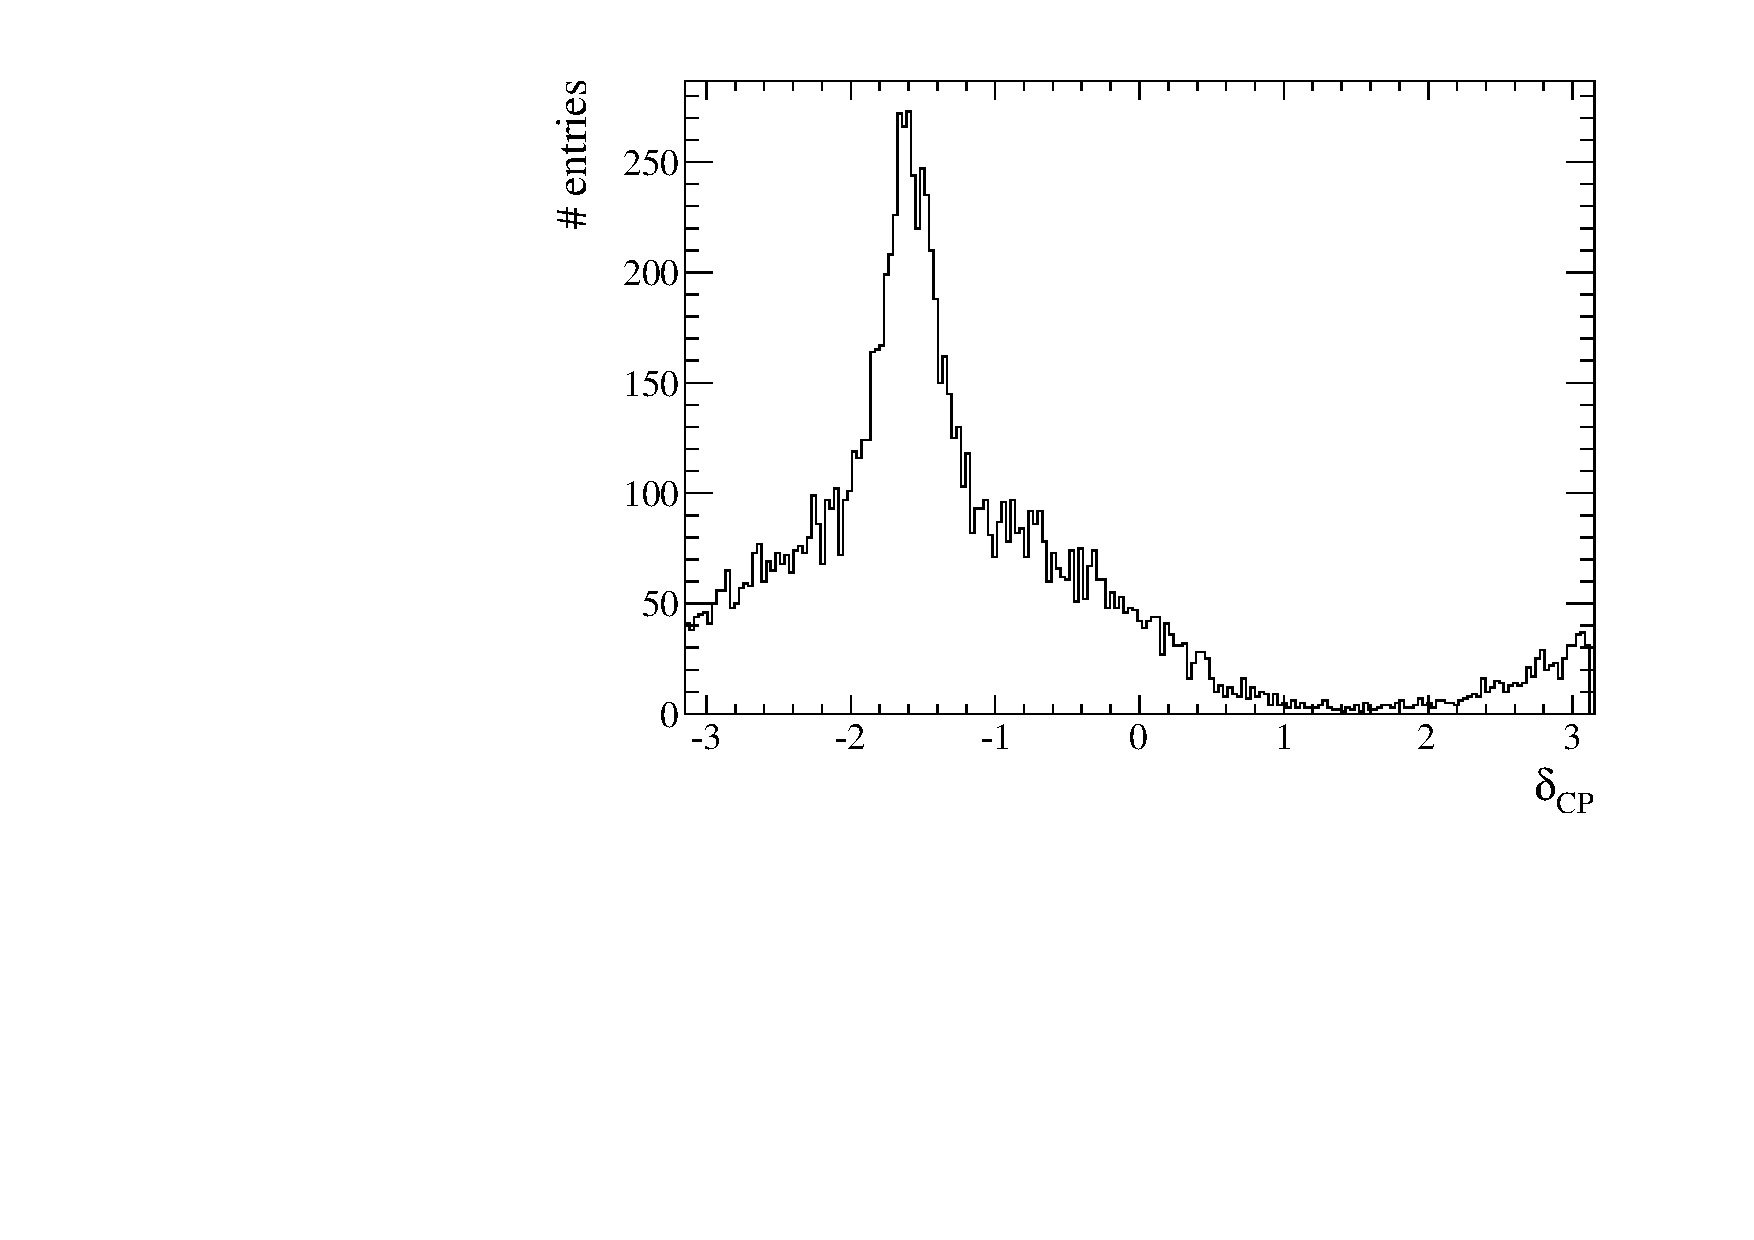
\includegraphics[width=0.9\textwidth]{./joint_plots/coverage_fc/coverage_run17c/Run17_cbestfit_deltacp_m1p571_normal.pdf}
\caption{Best-fit distribution of $\delta_{CP}$. $\delta_{CP}^{true} = -\pi/2$.}
\end{subfigure}
\begin{subfigure}[b]{0.49\textwidth}
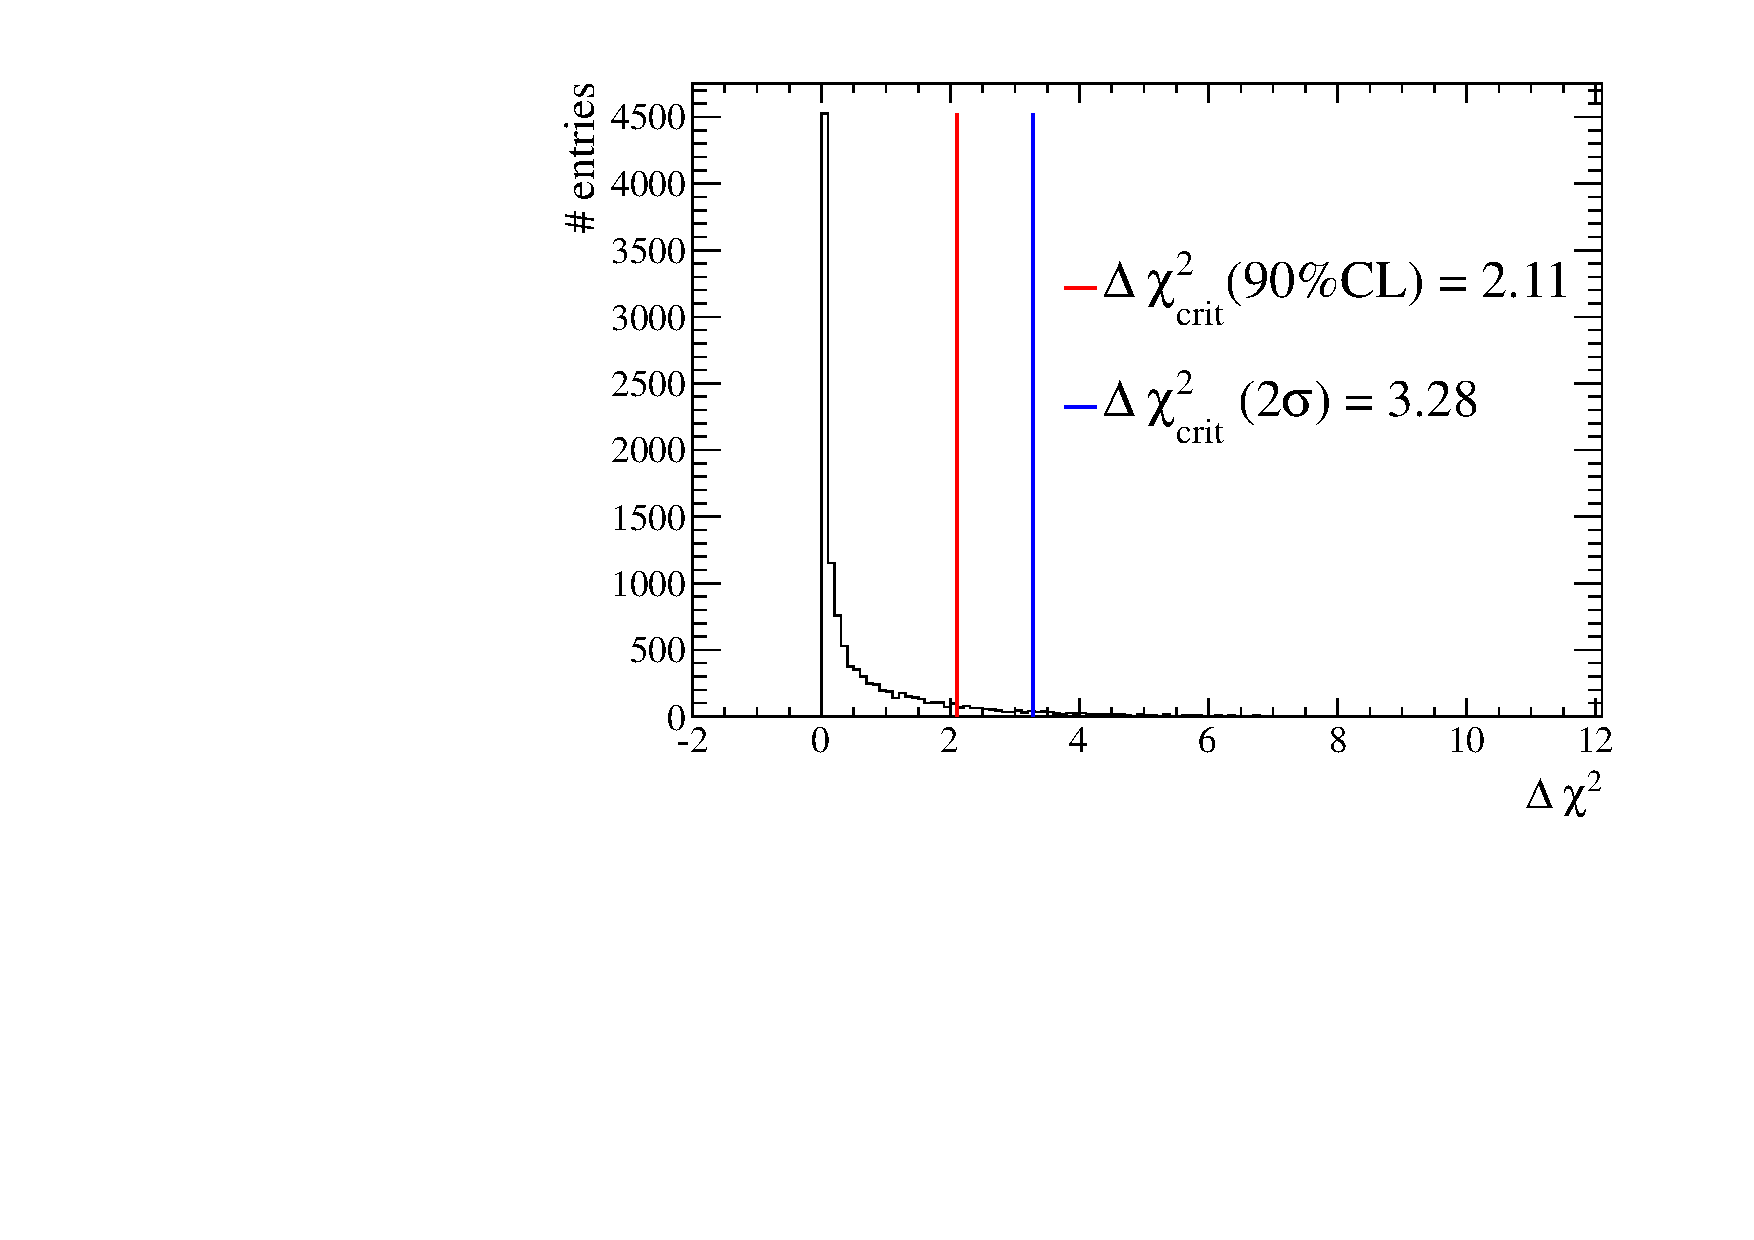
\includegraphics[width=0.9\textwidth]{./joint_plots/coverage_fc/coverage_run17c/Run17_deltachisq_glob_deltacp_m1p571_normal.pdf}
\caption{$\Delta \chi^2$ distribution.
$\delta_{CP}^{true} = -\pi/2$.}
\end{subfigure}
\begin{subfigure}[b]{0.49\textwidth}
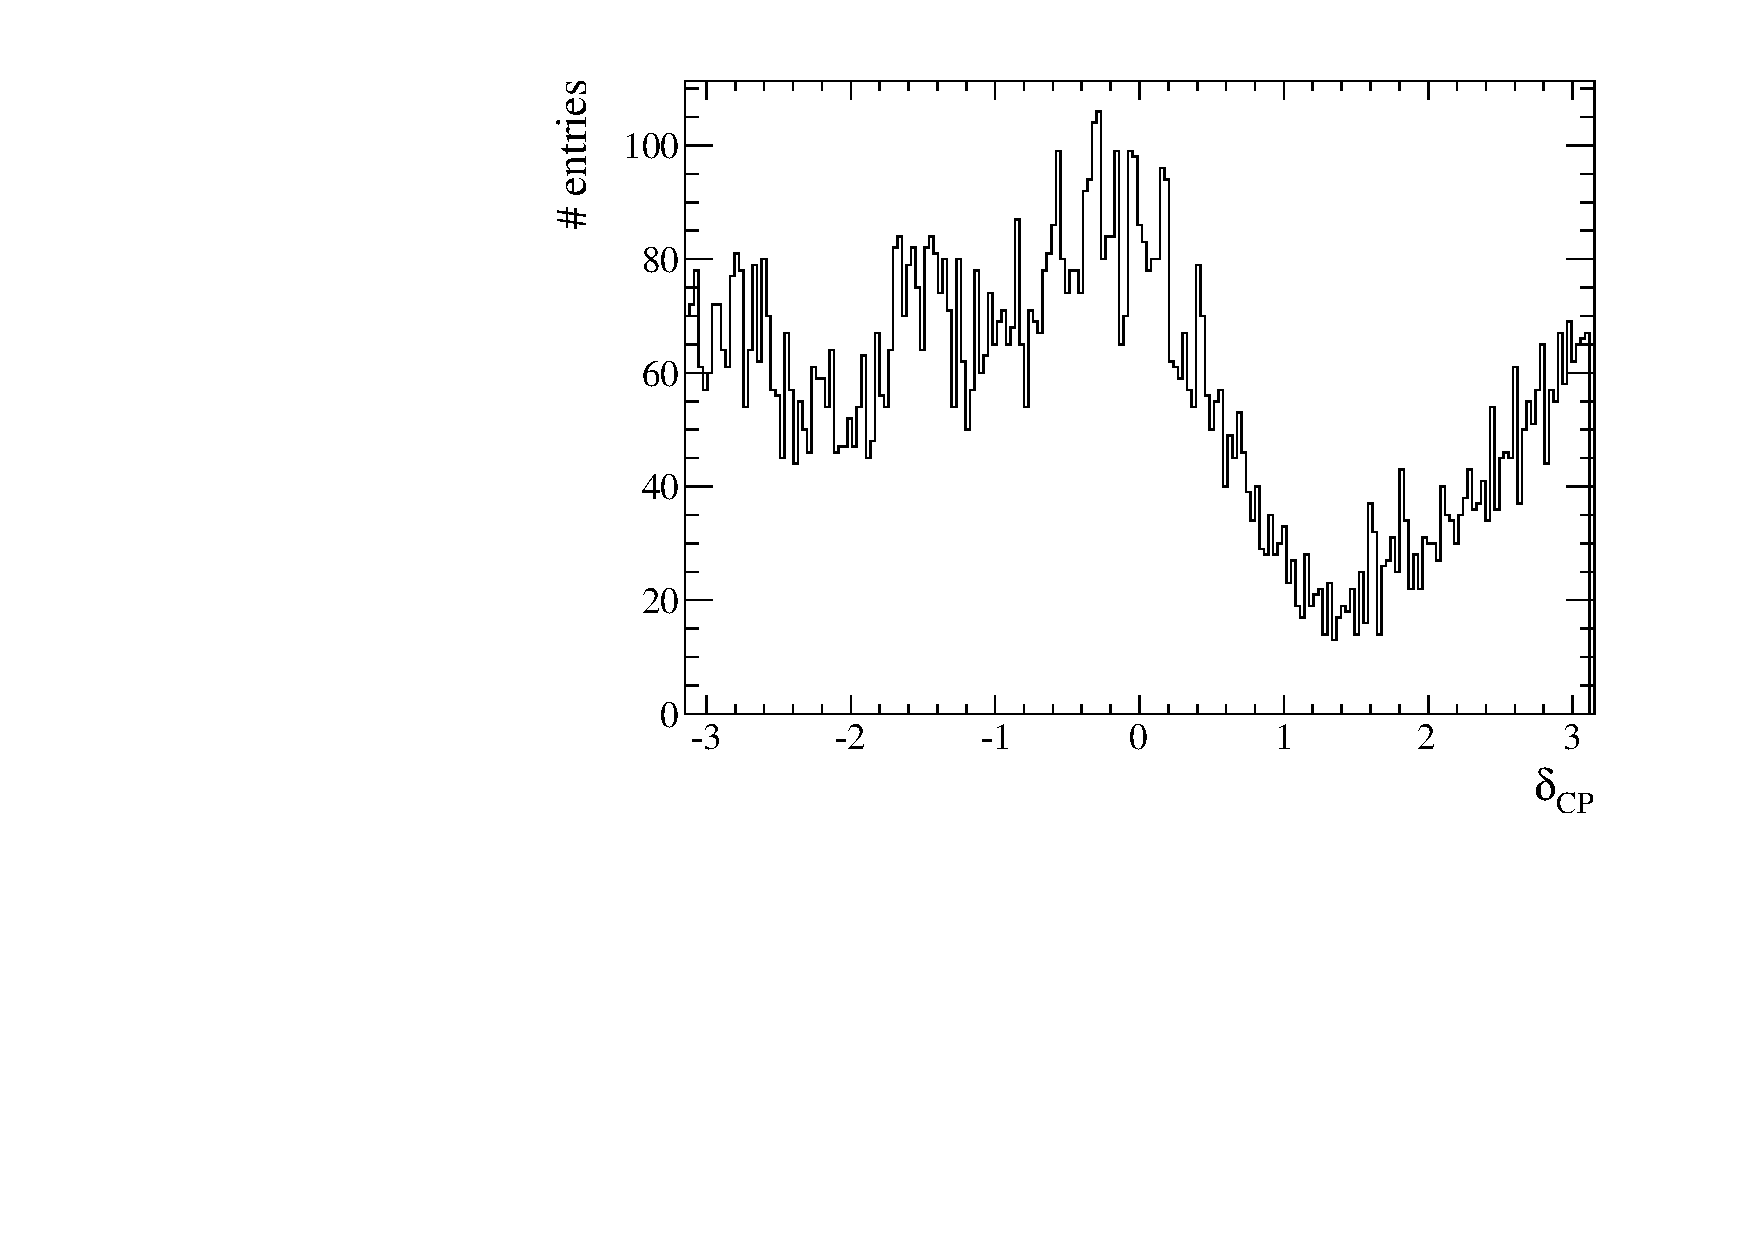
\includegraphics[width=0.9\textwidth]{./joint_plots/coverage_fc/coverage_run17c/Run17_cbestfit_deltacp_0_normal.pdf}
\caption{Best-fit distribution of $\delta_{CP}$. $\delta_{CP}^{true} = 0$.}
\end{subfigure}
\begin{subfigure}[b]{0.49\textwidth}
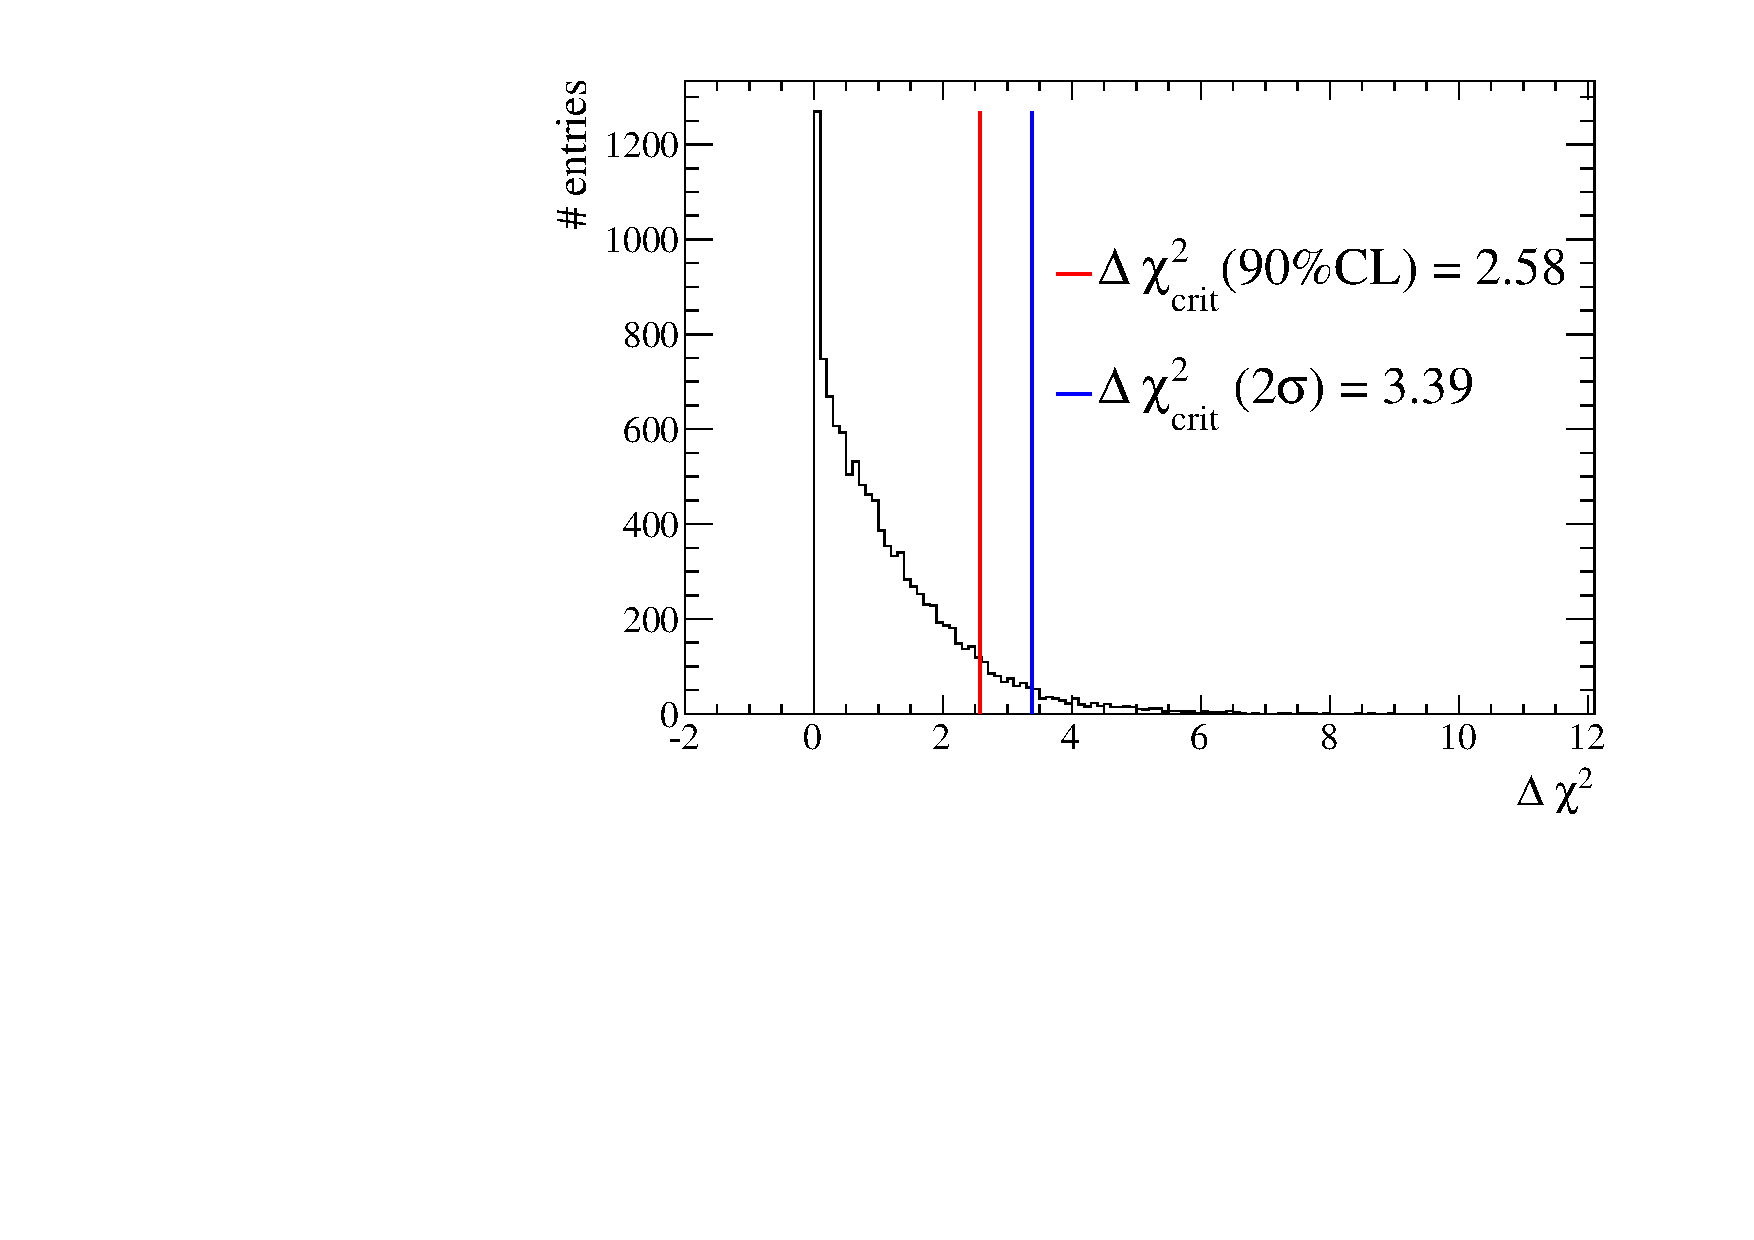
\includegraphics[width=0.9\textwidth]{./joint_plots/coverage_fc/coverage_run17c/Run17_deltachisq_glob_deltacp_0_normal.pdf}
\caption{$\Delta \chi^2$ distribution.
$\delta_{CP}^{true} = 0$.}
\end{subfigure}
\begin{subfigure}[b]{0.49\textwidth}
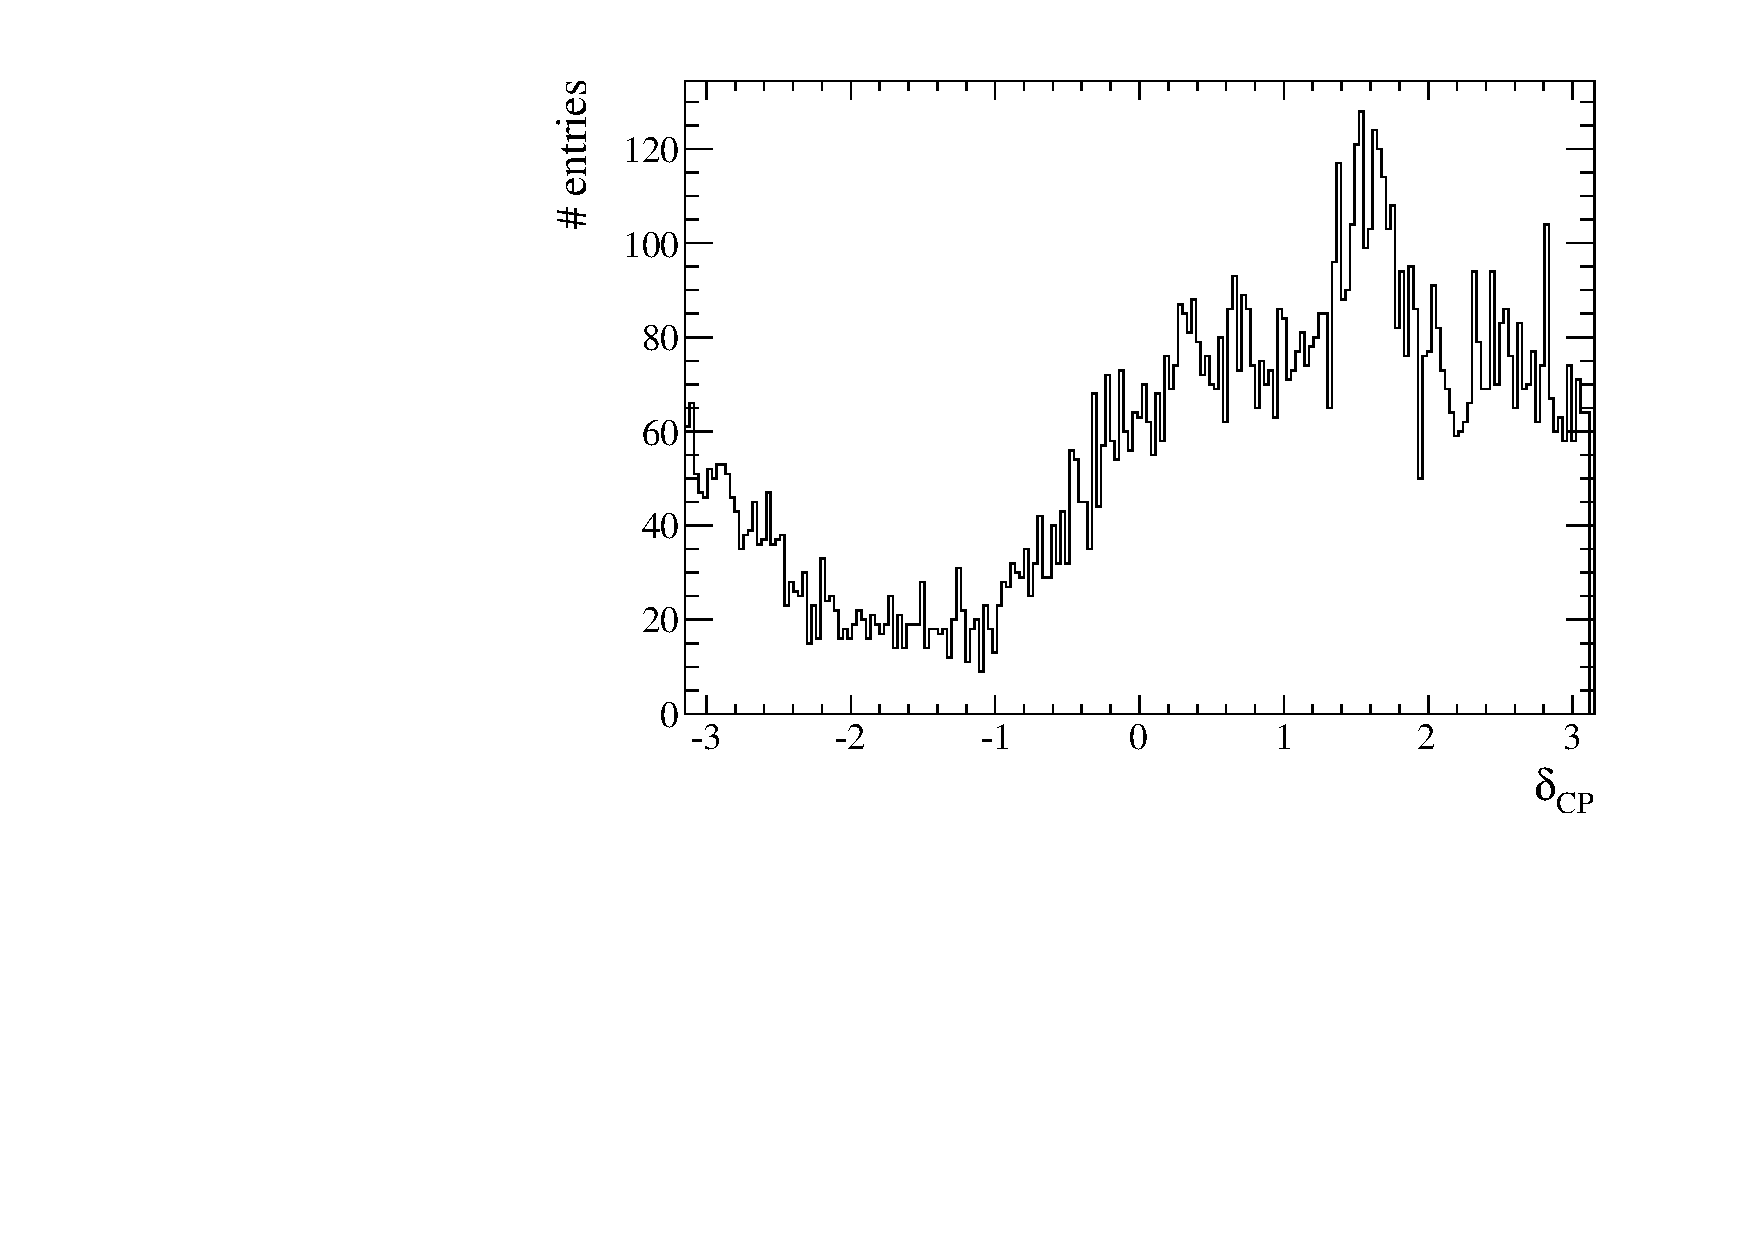
\includegraphics[width=0.9\textwidth]{./joint_plots/coverage_fc/coverage_run17c/Run17_cbestfit_deltacp_p1p571_normal.pdf}
\caption{Best-fit distribution of $\delta_{CP}$. $\delta_{CP}^{true} = +\pi/2$.}
\end{subfigure}
\begin{subfigure}[b]{0.49\textwidth}
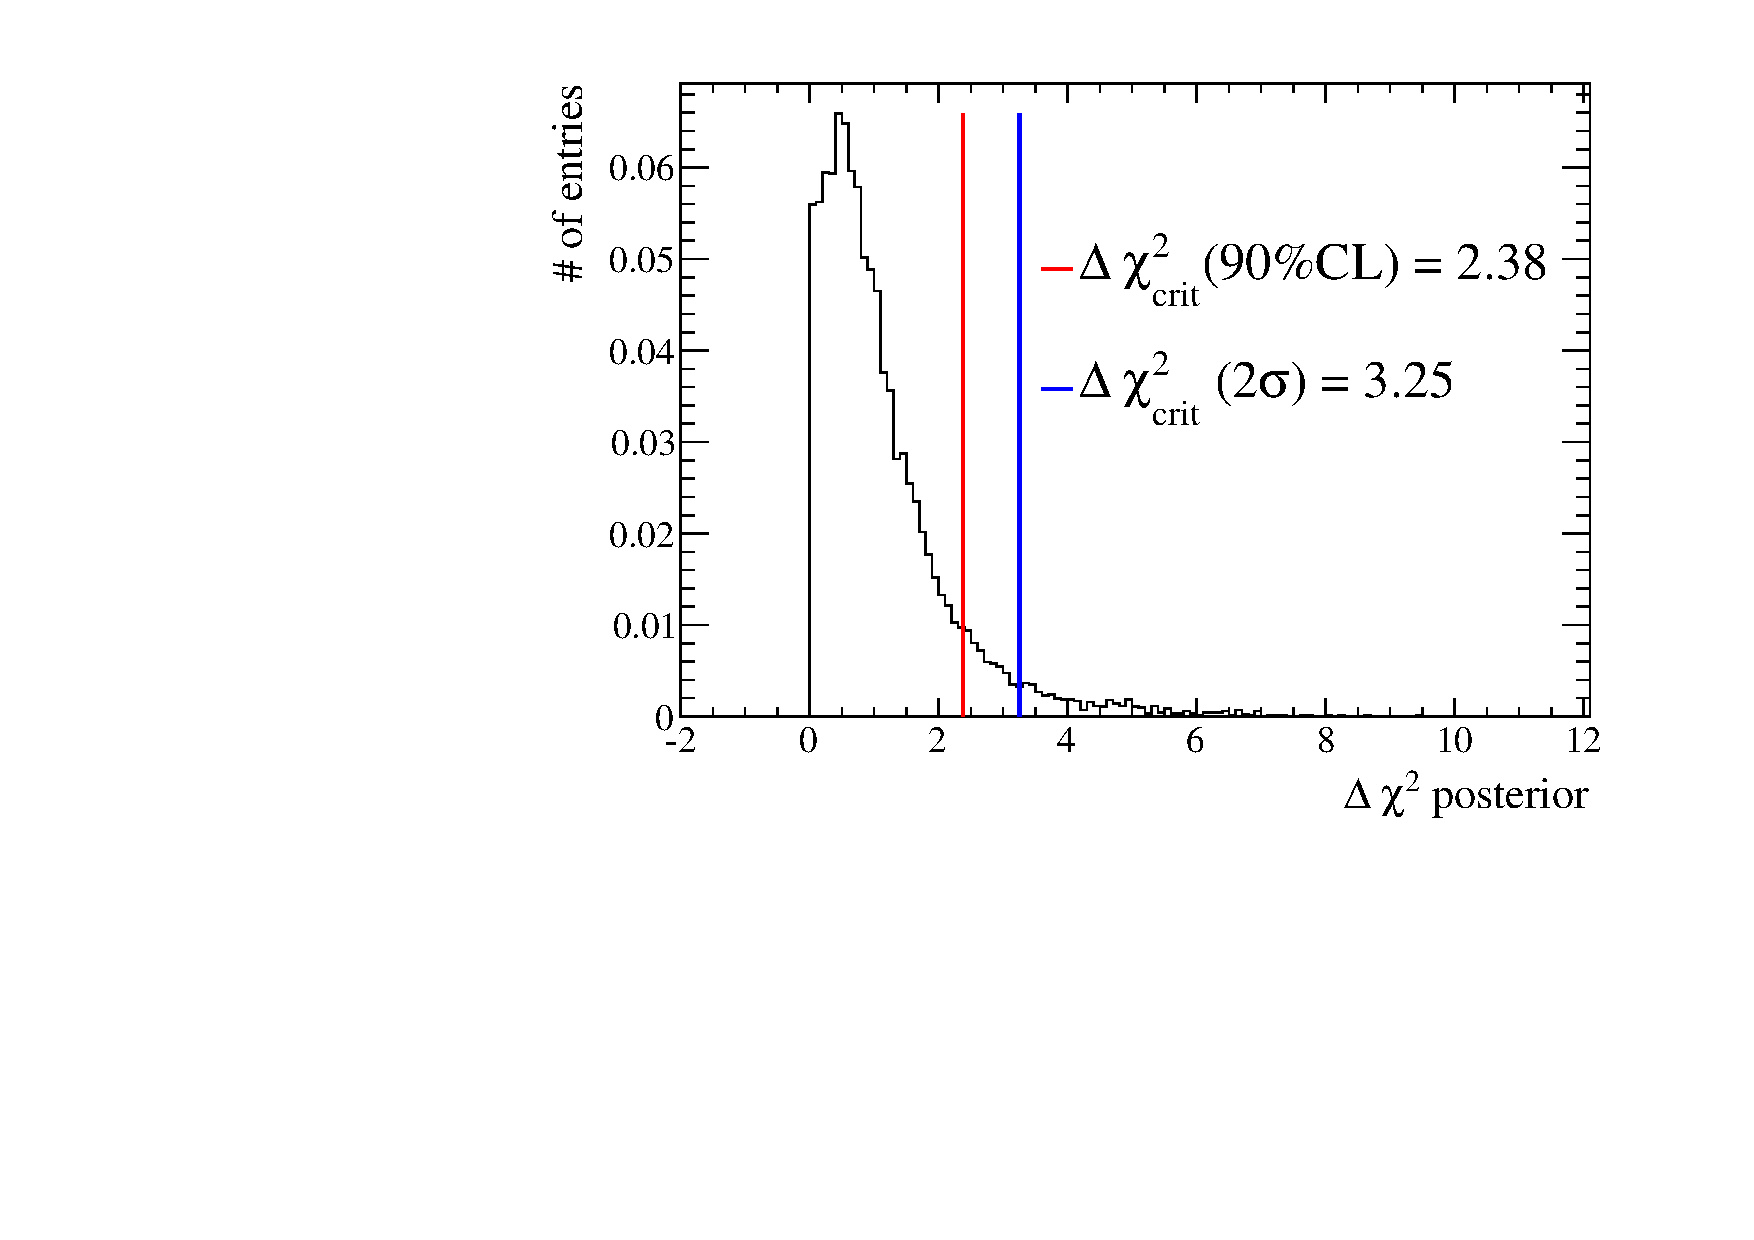
\includegraphics[width=0.9\textwidth]{./joint_plots/coverage_fc/coverage_run17c/Run17_deltachisq_glob_deltacp_p1p571_normal.pdf}
\caption{$\Delta \chi^2$ distribution.
$\delta_{CP}^{true} = +\pi/2$.}
\end{subfigure}
\caption {
Distributions of best-fit $\delta_{CP}$ (left) and $\Delta \chi^2$ (right).  
$10k$ toy experiments are performed
with true values of $\delta_{CP} = -\pi/2, 0, +\pi/2$, 
assuming normal hierarchy and applying the reactor constraint.
Both the mass hierarchy and $\delta_{CP}$ are profiled in the fit.
All the other oscillation parameters are marginalised.
The statistics corresponds to the Run 1-7c data set.
}
\label{fig:dchisq_bestfit_dcp_run17c}
\end{figure*}



\clearpage



%In \cref{fig:critval_comparision_run17b_run17c} the critical values obtained with the Feldman-Cousins method
%for both Run 1-6 and Run  1-7c statistic are shown.
%The critical values at both 90\% and $2\sigma$ CL are computed
%for both the mass hierarchies and the following true values of $\delta_{CP}$: 
%$-\pi$, -2.356, $-\pi/2$, -0.785, 0, +0.785, $+\pi/2$, -2.356, $+\pi$. 
%As already shown in \cref{tab:critval_0_pmhalfpi_run17c} and \cref{fig:dchisq_bestfit_dcp_run17c},
%the behavior of the critical values for Run 1-6 and Run 1-7c are quite similar, 
%given the fact that with Run 7c the additional amount of events is negligible in the neutrino mode $e$-like sample 
%(fewer than 0.5 event)
%and small in the antineutrino mode $e$-like sample (fewer than 3 events).



%\begin{figure*}[htb]
%\center
%\begin{subfigure}[b]{0.49\textwidth}
%%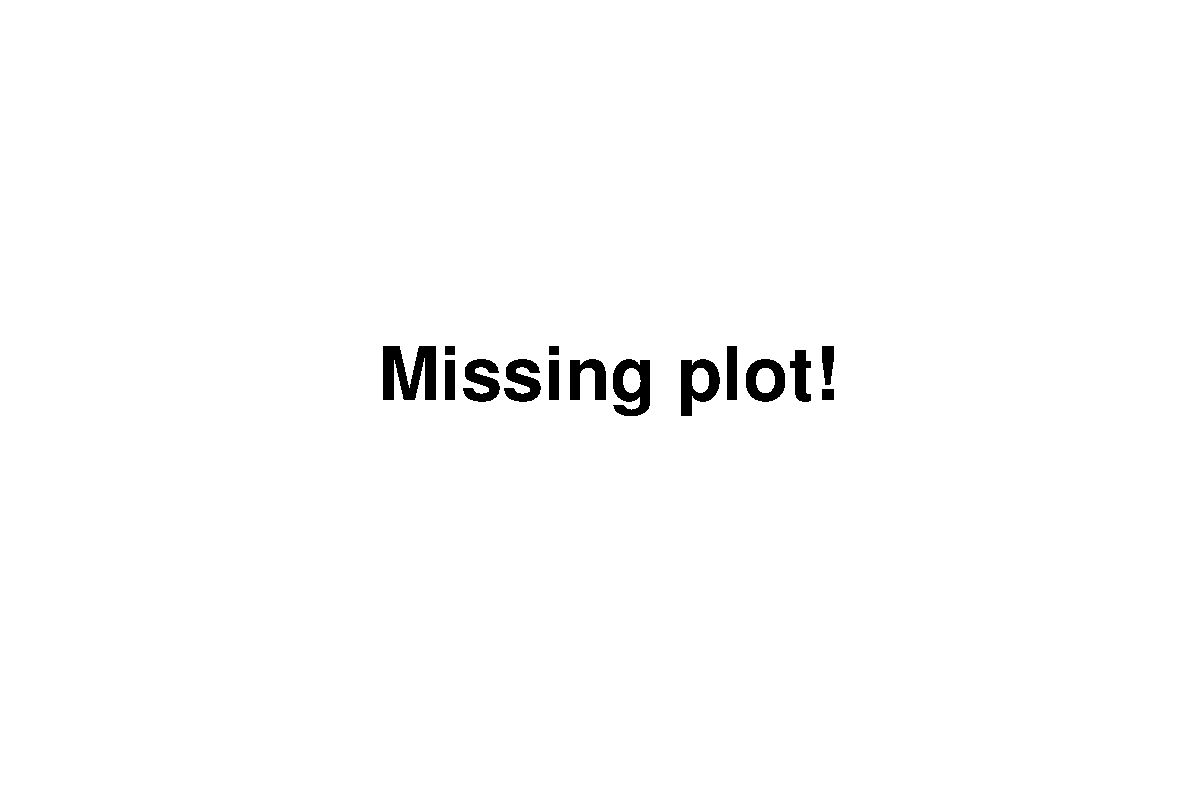
\includegraphics[width=0.9\textwidth]{./images/missing_plot-eps-converted-to.pdf}
%%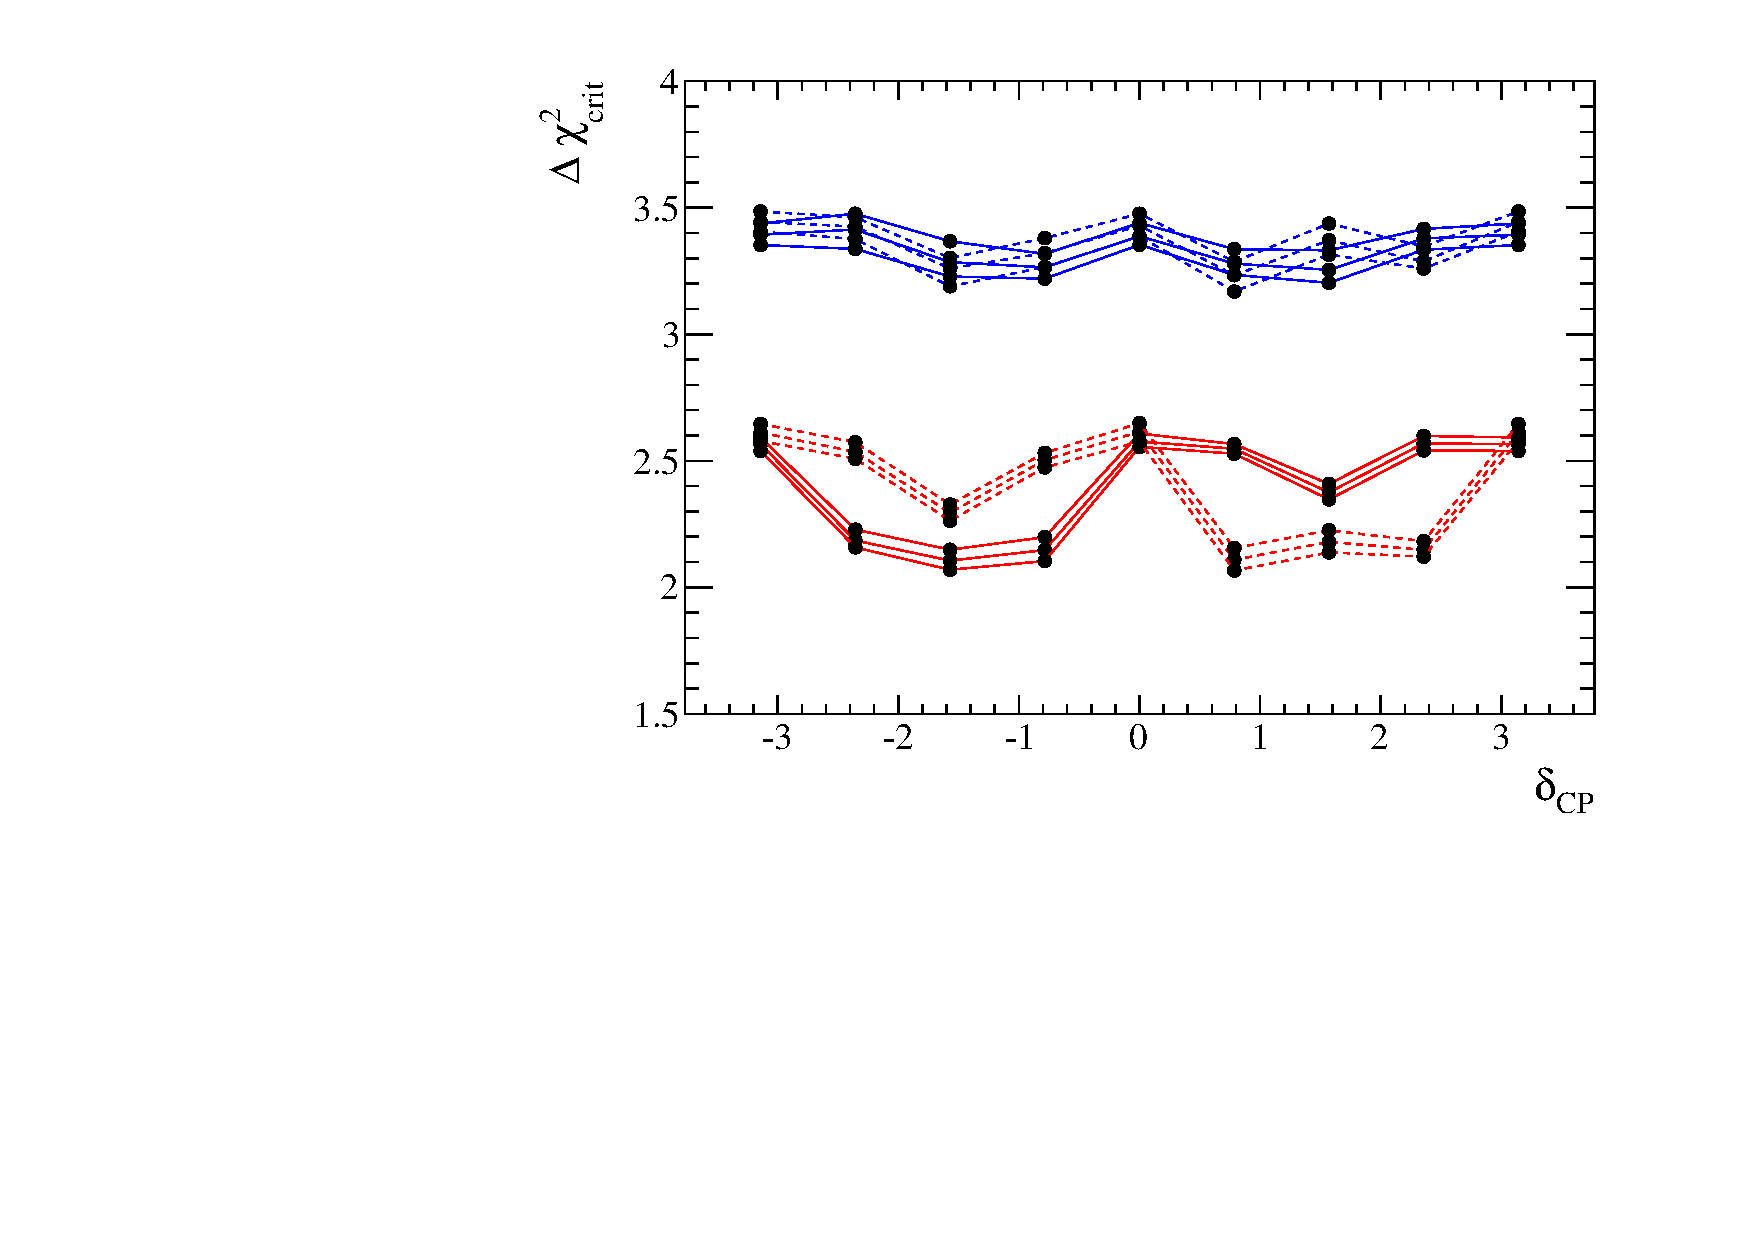
\includegraphics[width=0.9\textwidth]{./joint_plots/coverage_fc/fc_run17c/critical_values_run17c_fluxtun_run17b.pdf}
%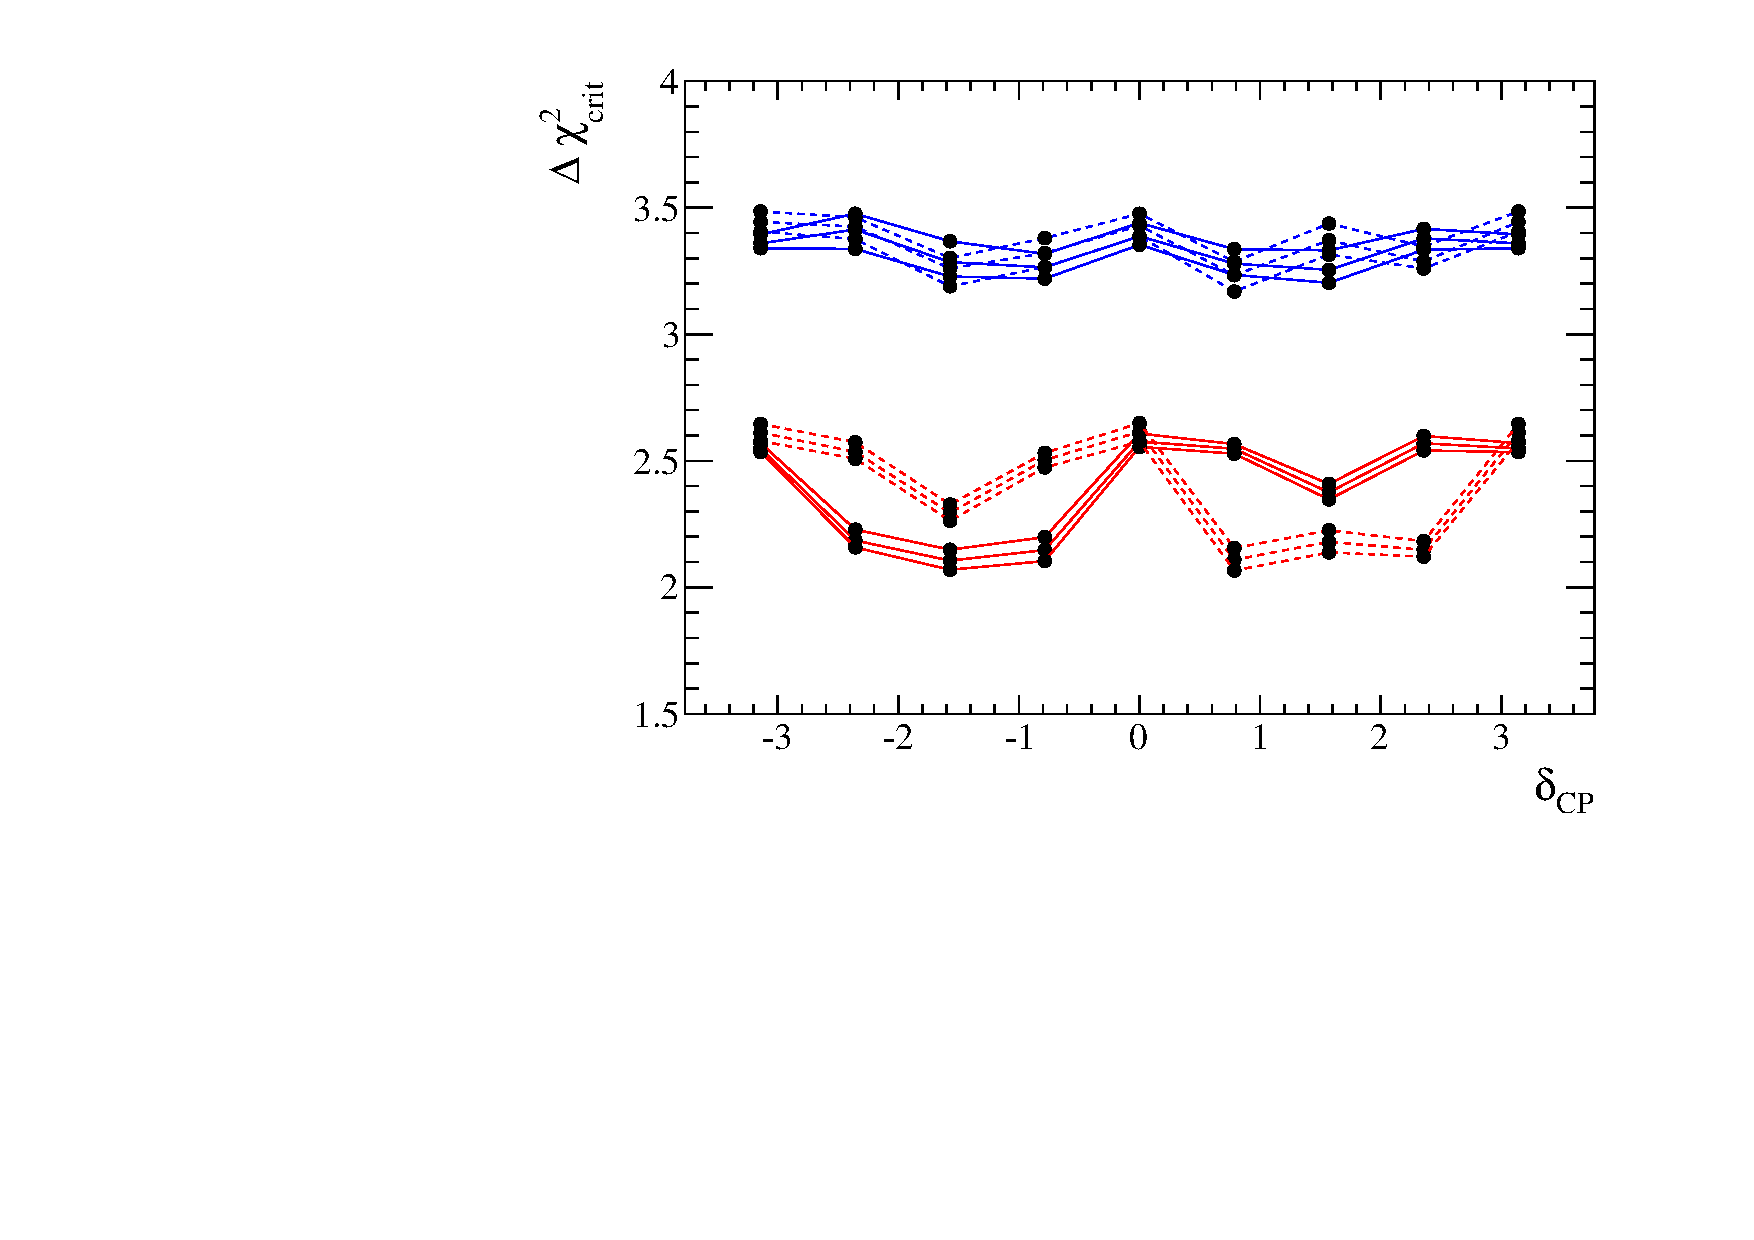
\includegraphics[width=0.9\textwidth]{./joint_plots/coverage_fc/fc_run17c/critical_values_run17c_fluxtun_merge_dcp_3p142.pdf}
%\caption{Critical values obtained with the Feldman-Cousins method for Run 1-7c statistic}
%\end{subfigure}
%\begin{subfigure}[b]{0.49\textwidth}
%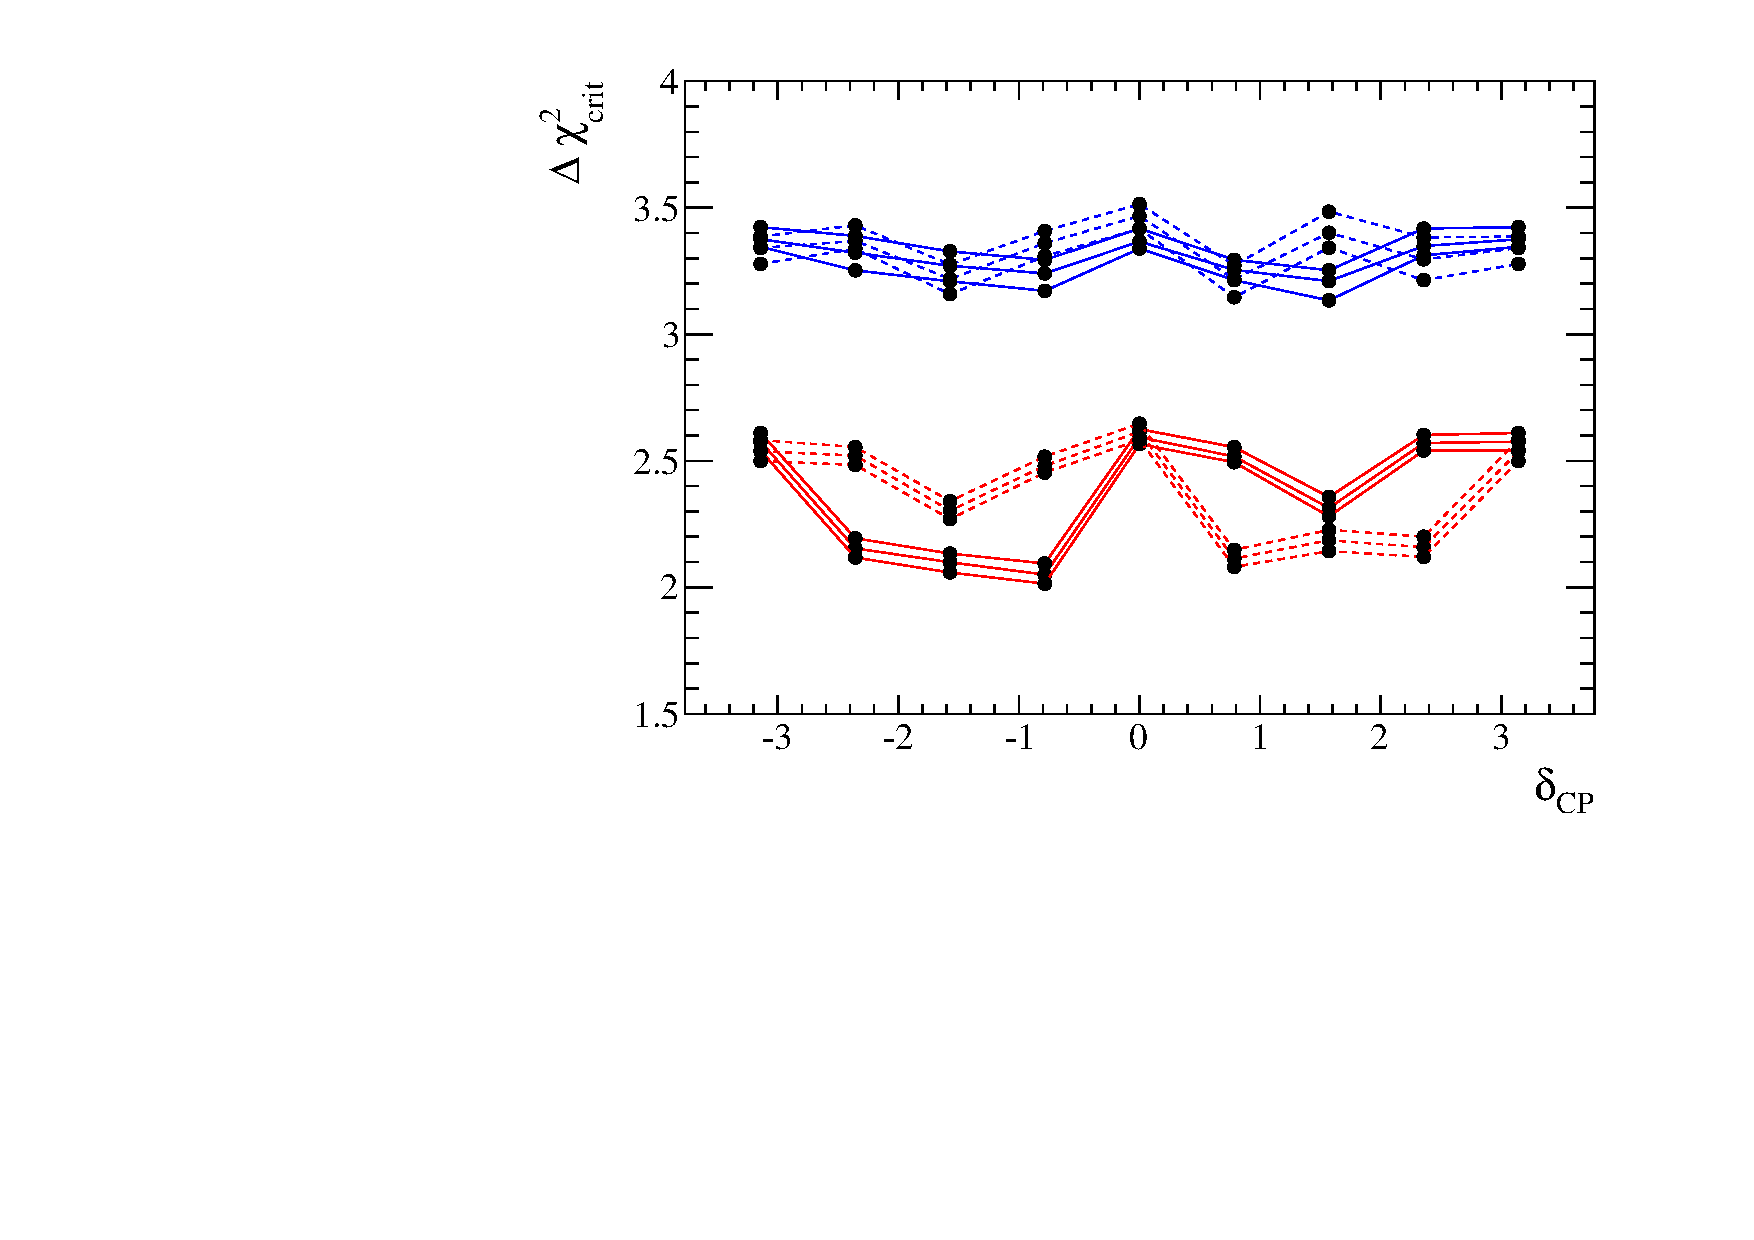
\includegraphics[width=0.9\textwidth]{./joint_plots/coverage_fc/fc_run17b/critical_values_fluxrun16.pdf}
%\caption{Critical values obtained with the Feldman-Cousins method for Run 1-7b statistic}
%\end{subfigure}
%\caption {
%Critical values obtained with the Feldman-Cousins method for Run 1-7c and Run 1-7b statistic
%for several true values of $\delta_{CP}$ and both normal (solid line) and inverted (dashed line) hierarchy.
%Both 90\% (red) and $2\sigma$ (blue) CL critical values are shown.
%About $10k$ toy experiments are performed for each point except $\delta_{CP} = \pi$ - normal hierarchy,
%for which $28k$ toy experiments are performed.
%All the other oscillation parameters are marginalised.
%The $\pm1 \sigma$ error on the critical values is shown as well
%and is represented by the lowest and highest set of critical values, with the same color of the central ones.
%}
%\label{fig:critval_comparision_run17b_run17c}
%\end{figure*}


\clearpage

\subsection{Validation of the minimisation algorithm}
\label{sec:minim_algorithm_run17c}

For each true value of $\delta_{CP}$, where the critical value is performed using the Feldman-Cousins method,
and normal hierarchy, 5000 fits were performed on fake data sets of the same type as used for Feldman-Cousins.
About all the fits except X found the global minimum.



\clearpage

%
\clearpage

\section {Results of the $\bar{\nu}/\nu$ joint analysis with the Run 1-7c dataset}
\label{sec:results}

The results of the Run 1-7c data set fit,
for an exposure 
of \TotalPotNuRunOneSevenC POT in neutrino mode
and
of \TotalPotNuBarRunOneSevenC POT in antineutrino mode, 
are shown in this chapter.
In \cref{fig:spectra_expVsdata_asimov_A_run17c} the predicted spectra of $\mu$-like and $e$-like samples
are compared to the observed data.
In \cref{tab:num_events_run17c} the expected and observed number of events in Run 1-7c data set are shown.
The predicted number of events are shown for the oscillation parameters in \cref{tab:osc_params_joint_asimov}
of Asimov data sets A and B.
%All the predicted and observed events are in good agreement.

The comparison of the confidence intervals obtained by the fit of the Run 1-7c data set
among all the oscillation analysis groups is shown in \cite{Mach3JointFitCCPi}.

\begin{figure}
\center
\begin{subfigure}[b]{0.49\textwidth}
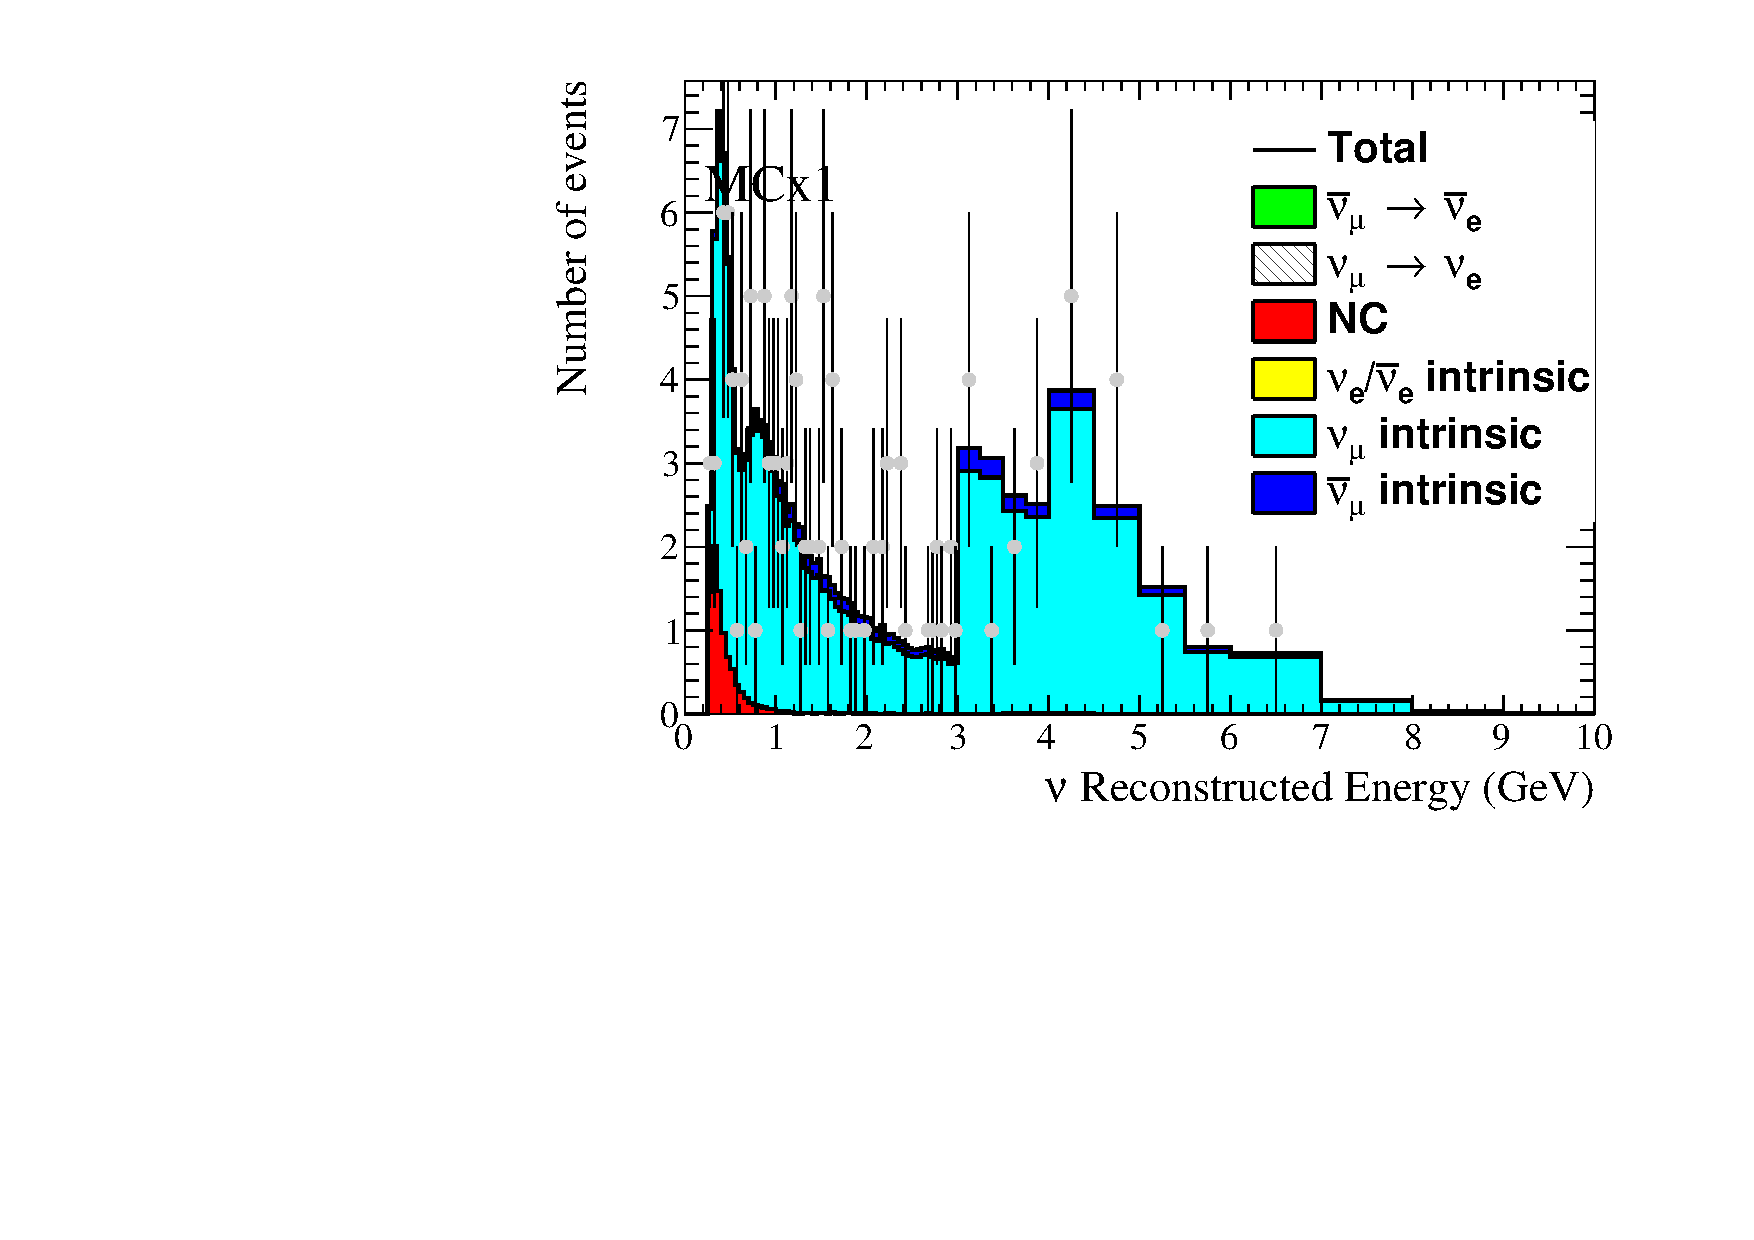
\includegraphics[width=0.9\textwidth]{./joint_plots/data/ccpi/cErecoTotFlavMode_1Rmu.pdf} 
\caption{Muon-like, neutrino mode}
\end{subfigure}
\begin{subfigure}[b]{0.49\textwidth}
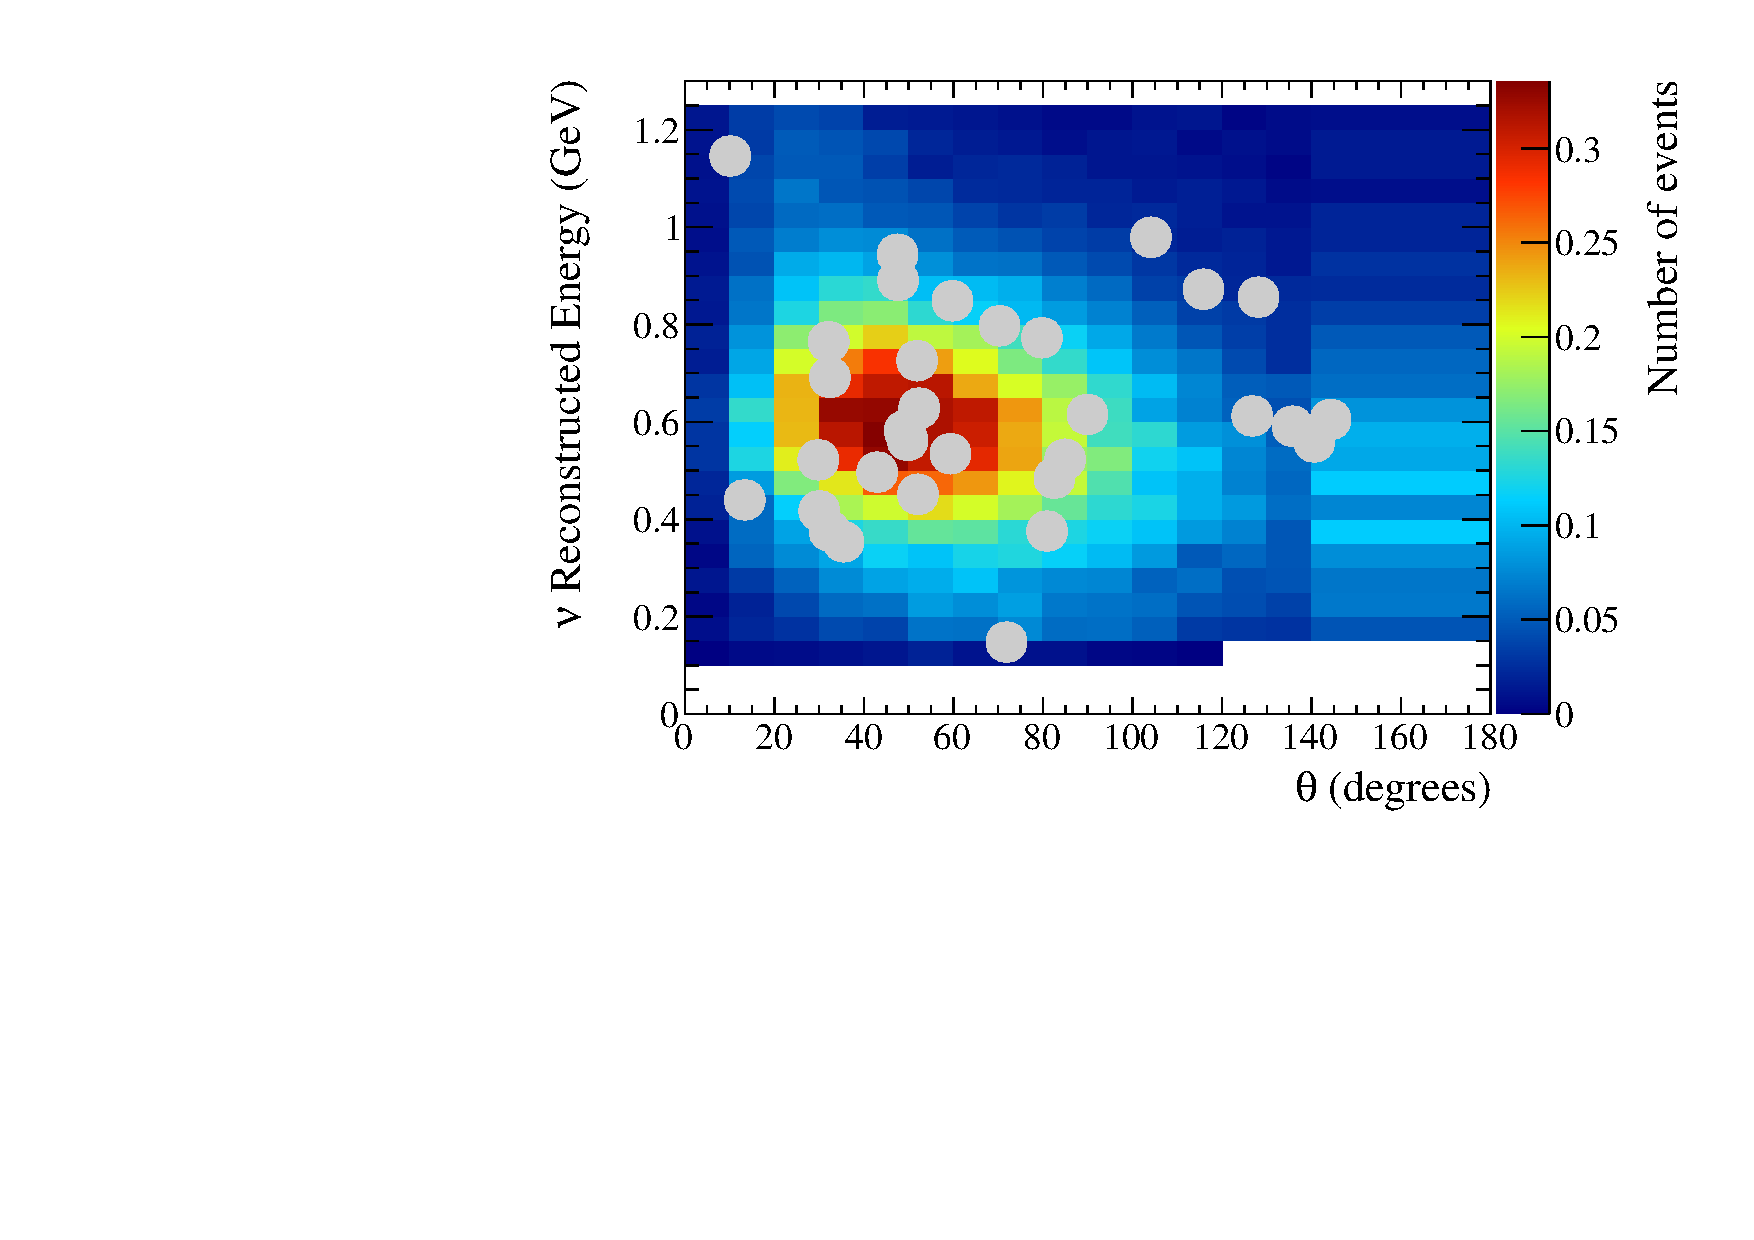
\includegraphics[width=0.9\textwidth]{./joint_plots/data/ccpi/cErecoVsQ2Tot_1Re.pdf} 
\caption{Electron-like, neutrino mode}
\end{subfigure}
\begin{subfigure}[b]{0.49\textwidth}
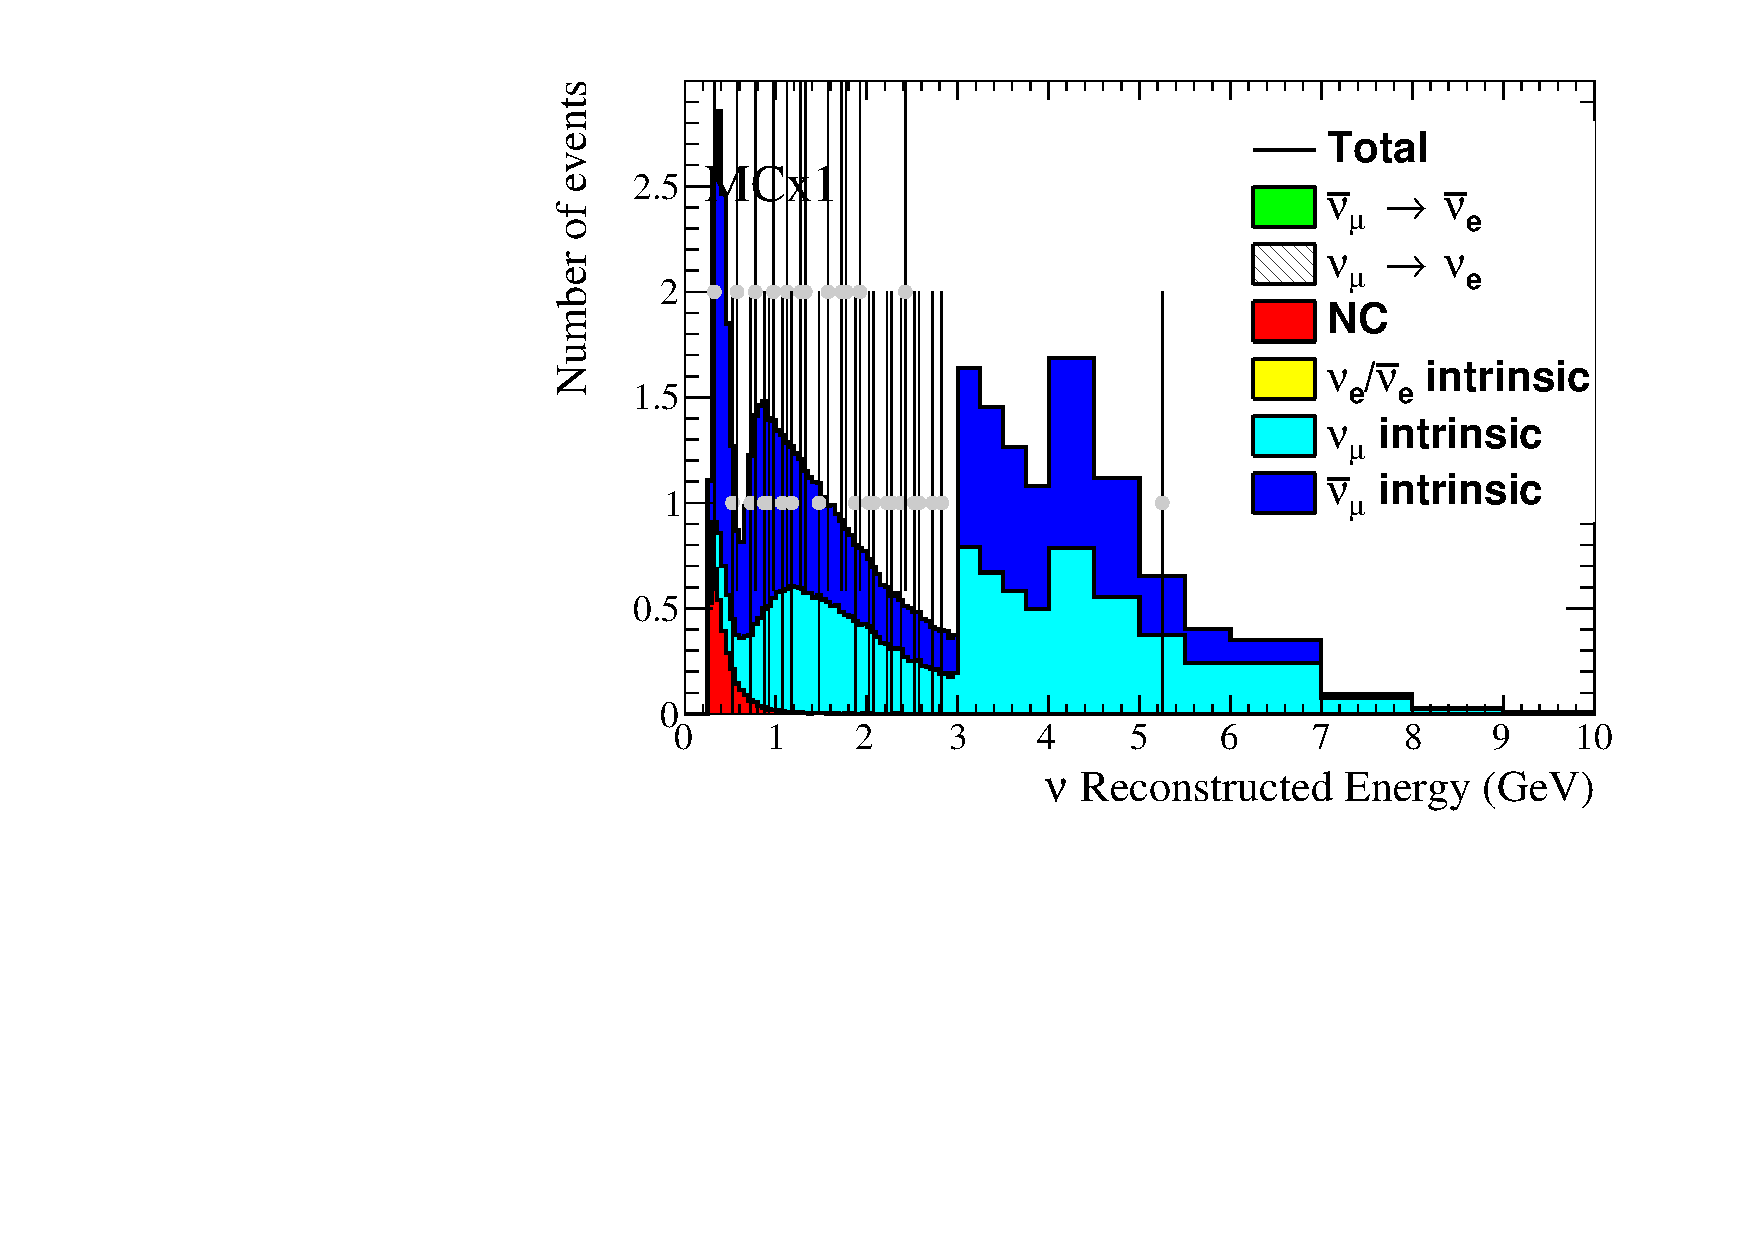
\includegraphics[width=0.9\textwidth]{./joint_plots/data/ccpi/cErecoTotFlavMode_RHC1Rmu.pdf} 
\caption{Muon-like, antineutrino mode}
\end{subfigure}
\begin{subfigure}[b]{0.49\textwidth}
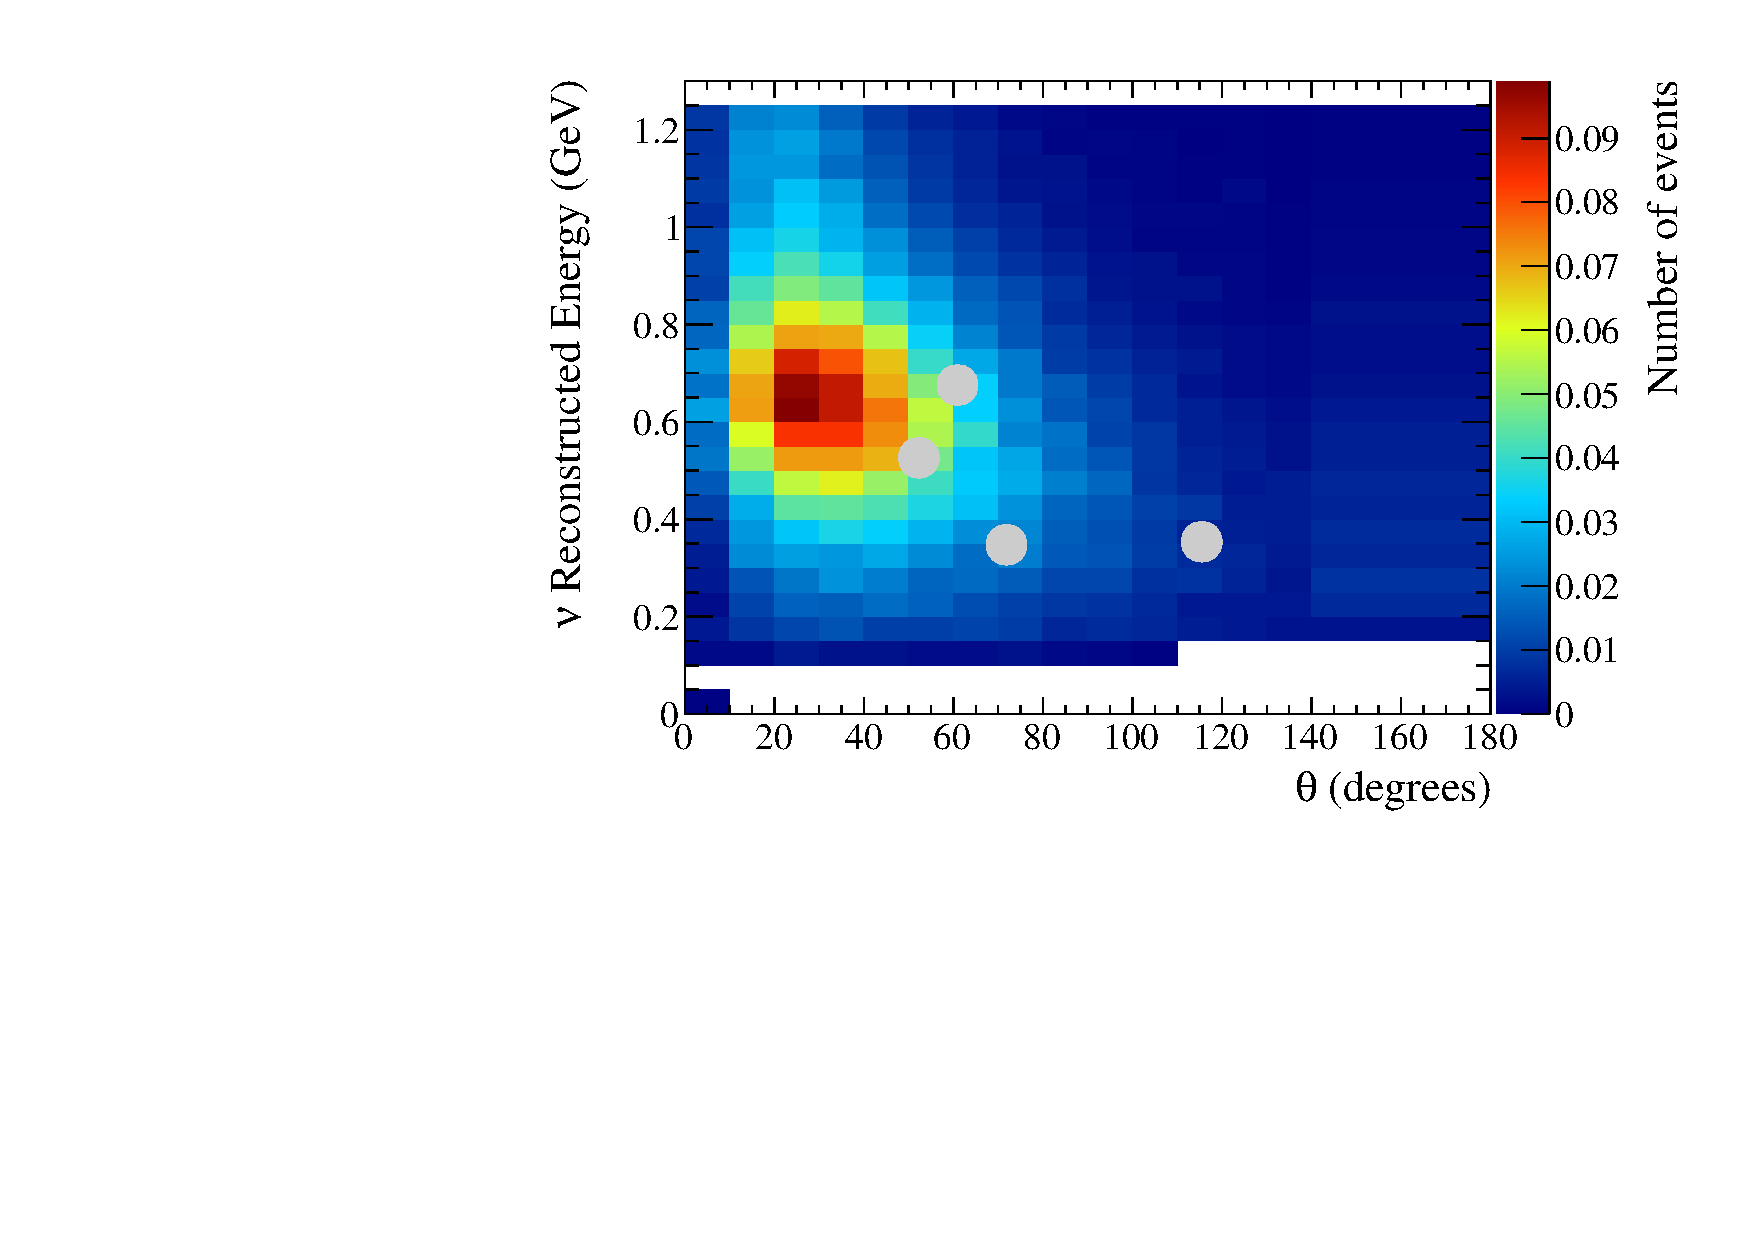
\includegraphics[width=0.9\textwidth]{./joint_plots/data/ccpi/cErecoVsQ2Tot_RHC1Re.pdf} 
\caption{Electron-like, antineutrino mode}
\end{subfigure}
\begin{subfigure}[b]{0.49\textwidth}
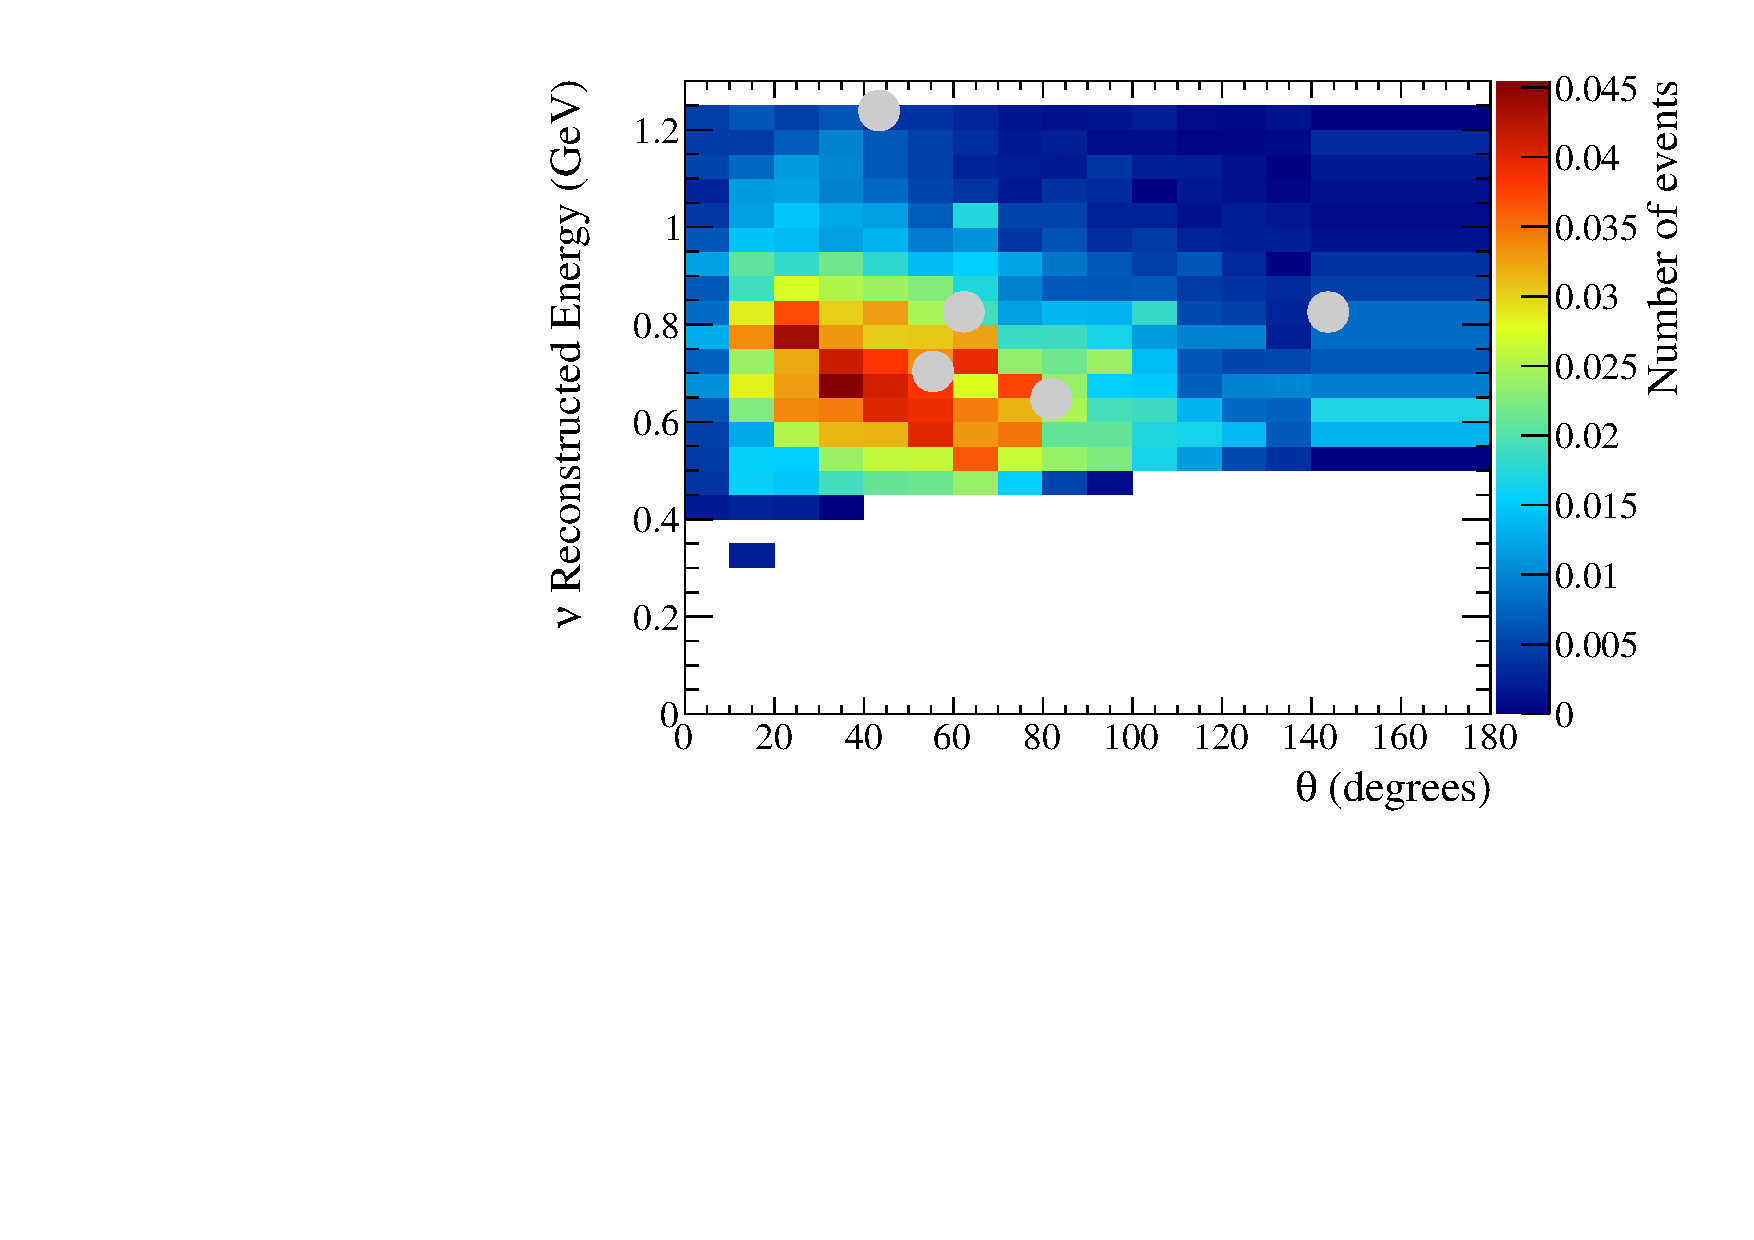
\includegraphics[width=0.9\textwidth]{./joint_plots/data/ccpi/cErecoVsQ2Tot_MultiRe.pdf} 
\caption{cc$\pi^+$-like, neutrino mode}
\end{subfigure}
\caption {
The predicted spectra compared to the Run 1-7c dataset (dots),
which corresponds to an exposure 
of \TotalPotNuRunOneSevenC POT in neutrino mode
and
of \TotalPotNuBarRunOneSevenC POT in antineutrino mode,
are shown.
The expected distribution corresponds to the oscillation parameters of the Asimov data set A shown in \cref{tab:osc_params_joint_asimov}.
The spectra were generated with the systematic parameters measured with the ND280 data 
shown in \cref{tab:banff_uncertainties_flux_fhc},~\ref{tab:banff_uncertainties_flux_rhc},
~\ref{tab:banff_uncertainties_xsec} 
and the nominal Super-K systematic parameters shown in \cref{tab:banff_uncertainties_skdetfsi}.
}
\label{fig:spectra_expVsdata_asimov_A_run17c}
\end{figure}




% Table summarizing the # of observed events in Run 1-6

\begin{table}[htb]
\centering
\begin{tabular}{| c | c | c | c | c | c | c | c |}
\hline
Beam mode	& Sample		& Exp. Asimov A  	& Exp. Asimov A	& Exp. Asimov B	& Exp. Not Osc			& Observed 	& Best fit\\
			& 			& 			  	& ($\delta_{CP}=0$)	& 				& 					& 		 	& (reactors) \\
\hline
neutrino	 	& $\mu$-like 	&135.815			& 135.459			& 140.724	 		& 521.777				& 135 		& 135.255 \\
neutrino 		& $e$-like  	& 28.687 			& 24.170			& 21.524			& 6.147				& 32 			& 28.880 \\
antineutrino 	& $\mu$-like 	& 64.205			& 64.059			& 65.597			& 184.837				& 66 			& 63.870 \\
antineutrino 	& $e$-like 	& 6.004			& 6.902			& 6.252			& 2.335				& 4 			& 6.114 \\
neutrino 		& cc$\pi^+$-like & 3.126 			& 2.744			& 2.511			& 3.258				& 5 			& xxxx \\

\hline
\end{tabular}
\caption{
The observed, expected and best-fit number of events in Run 1-7c data set
for an exposure
of \TotalPotNuRunOneSevenC POT in neutrino mode
and
of \TotalPotNuBarRunOneSevenC POT in antineutrino mode
are shown 
for each selected sample.
The prediction is produced using the BANFF tuning
and the oscillation parameters shown in \cref{tab:osc_params_joint_asimov}.
The total number of events of the best-fit spectra is obtained by using \cref{eq:bestfit_spectrum_marg}.
}
\label{tab:num_events_run17c}
\end{table}













%--------------------------------------------------------------------------------------
%
% 1-dimensional chisq & best-fit
%
%--------------------------------------------------------------------------------------

\subsection {1-dimensional $\chi^2$ distributions and best-fit}
\label{sec:chisq_1d_run17c}


% 1-dimensional contours

1-dimensional $\chi^2$ distributions as in \cref{sec:sensi} are produced
and shown in \cref{fig:joint_data_fit_1d_run17c}.
The best-fit value of $\delta_{CP}$ when the reactor constraint is applied is -1.728
similar to that of the 1Ring sample analysis.
%, i.e. -1.854 (see \cref{tab:joint_bestfit}), but closer to $-\pi/2$ (i.e. -1.571).
 

\begin{figure*}[htb]
\center
\begin{subfigure}[b]{0.49\textwidth}
\includegraphics[width=0.9\textwidth]{joint_plots/data_contours/Run17c/1D/dcp_reactor.pdf}
\caption{$\delta_{CP}$ with reactor constraint}
\label{fig:dcp_fit_with_reactor_data}
\end{subfigure}
\begin{subfigure}[b]{0.49\textwidth}
%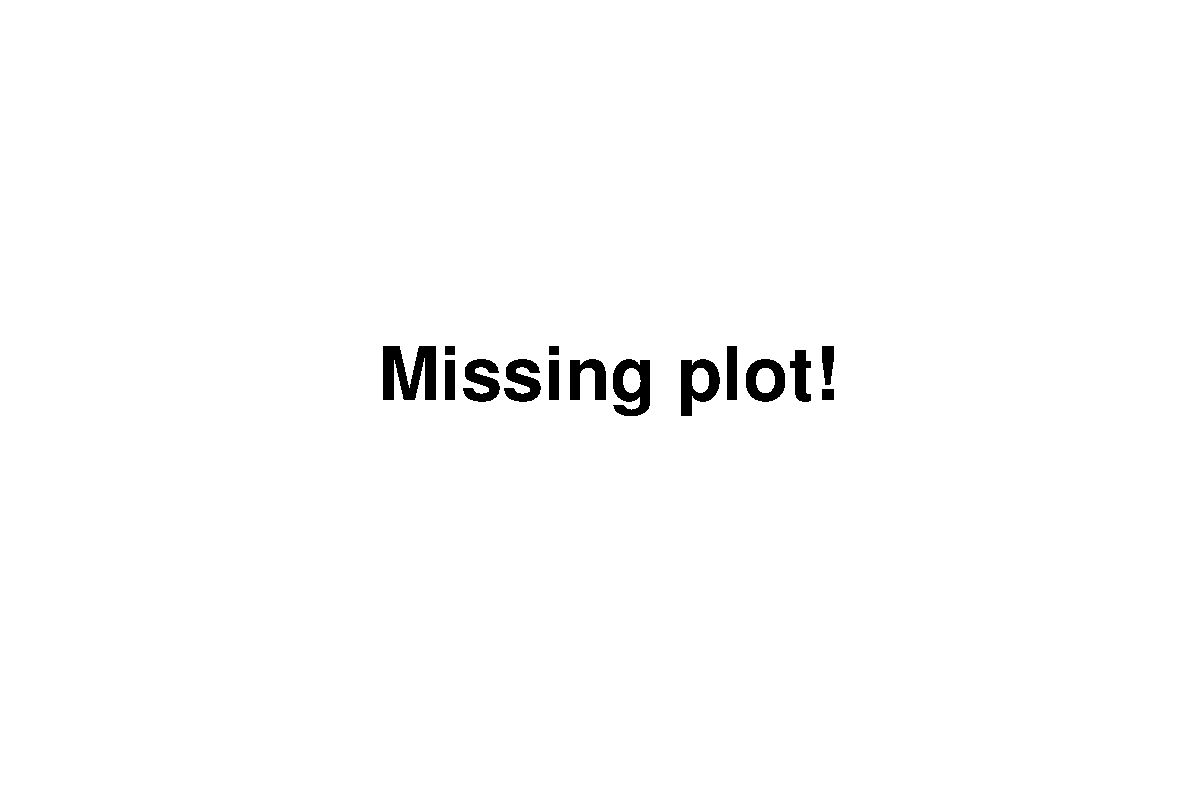
\includegraphics[width=0.9\textwidth]{./images/missing_plot-eps-converted-to.pdf}
\includegraphics[width=0.9\textwidth]{joint_plots/data_contours/Run17c/1D/dcp.pdf}
\caption{$\delta_{CP}$ with T2K data only}
\end{subfigure}
\begin{subfigure}[b]{0.49\textwidth}
%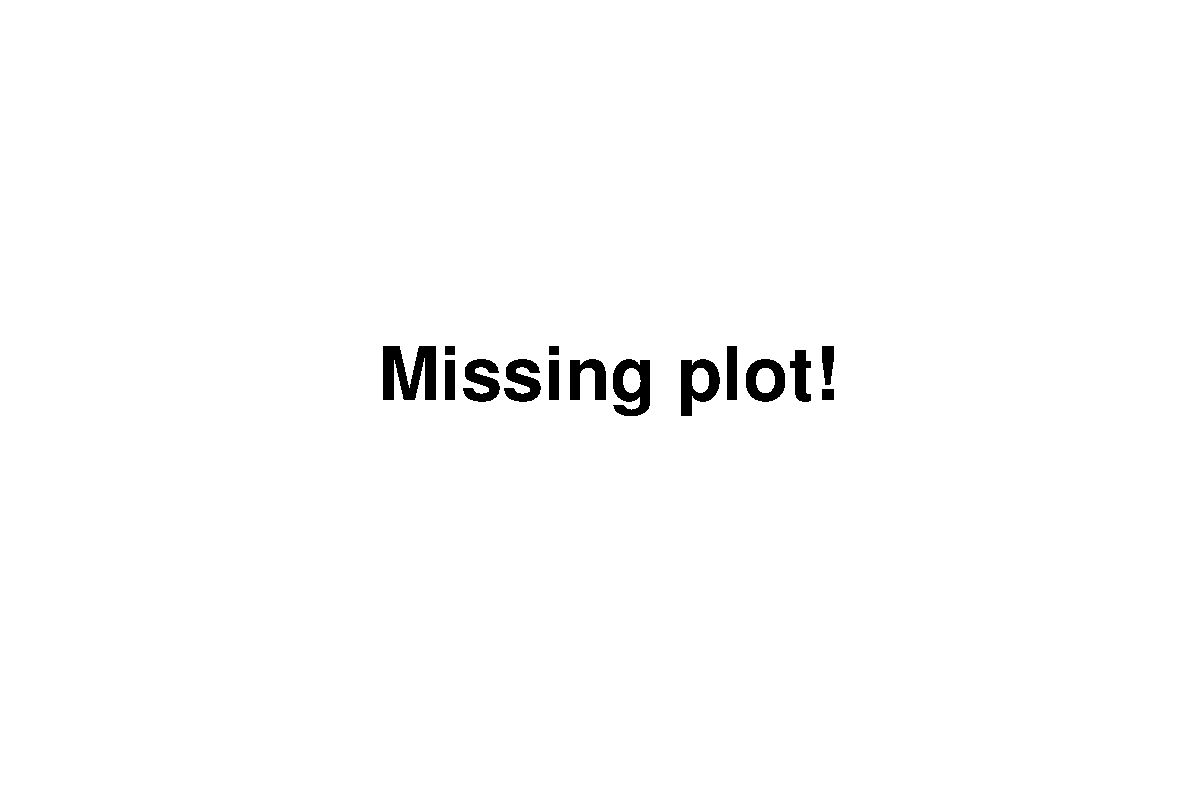
\includegraphics[width=0.9\textwidth]{./images/missing_plot-eps-converted-to.pdf}
\includegraphics[width=0.9\textwidth]{joint_plots/data_contours/Run17c/1D/ss13.pdf}
\caption{$\sin^2 \theta_{13}$ with T2K data only}
\end{subfigure}
\begin{subfigure}[b]{0.49\textwidth}
\includegraphics[width=0.9\textwidth]{joint_plots/data_contours/Run17c/1D/ss23.pdf}
\caption{$\sin^2 \theta_{23}$ with reactor constraint}
\end{subfigure}
\begin{subfigure}[b]{0.49\textwidth}
\includegraphics[width=0.9\textwidth]{joint_plots/data_contours/Run17c/1D/dmsq.pdf}
\caption{$\Delta m^2_{32}$ ($\Delta m^2_{13}$) with reactor constraint}
\end{subfigure}
\caption{
Measured $\Delta \chi^2$ distributions
with the full Run 1-7c data set.
Both normal (red) and inverted (blue) hierarchies are shown. 
The \emph{constant} $\Delta \chi^2$ method is used. %(see \cref{app:method_cl}).
Both normal and inverted hierarchy $\Delta \chi^2$ distributions are shifted with respect to the same global minimum. 
All the oscillation parameters which are not parameters of interest
are marginalised using the prior distributions shown in \cref{tab:marg_binnning}.
The measured $\Delta \chi^2$ distribution as a function of $\sin^2 \theta_{13}$ is compared
with the value given by the global analysis of the reactor measurements,
$\sin^2 \theta_{13} = 0.0219 \pm 0.0012 $
\cite{pdg_2014},
shown by the yellow bar.
}
\label{fig:joint_data_fit_1d_run17c}
\end{figure*}

%
% Neutrino only Vs AntiNeutrino only
%
%In \cref{fig:joint_dcp_nu_nubar}
%the $\chi^2$ distributions as a function of $\delta_{CP}$
%with reactor constraint
%is obtained by 
%running the analysis using either only neutrino 
%or antineutrino mode samples for the Run 1-6 data set,
%in order to check the compatibility of neutrino and antineutrino mode data.
%The result is mainly driven by the excess of the observed number
%of events in $e$-like neutrino mode sample compared to what is expected.
%Though the significance given by the antineutrino mode samples is still low,
%also given by the fact that $\sin^2 \theta_{23}$ is not constrained 
%by the antineutrino mode $\mu$-like sample
%as much as by  
%the neutrino mode $\mu$-like sample,
%it is interesting to note that the antineutrino data also prefer 
%a value of $\delta_{CP}$ close to $-\pi / 2$.
%
%\begin{figure*}[htb]
%\center
%%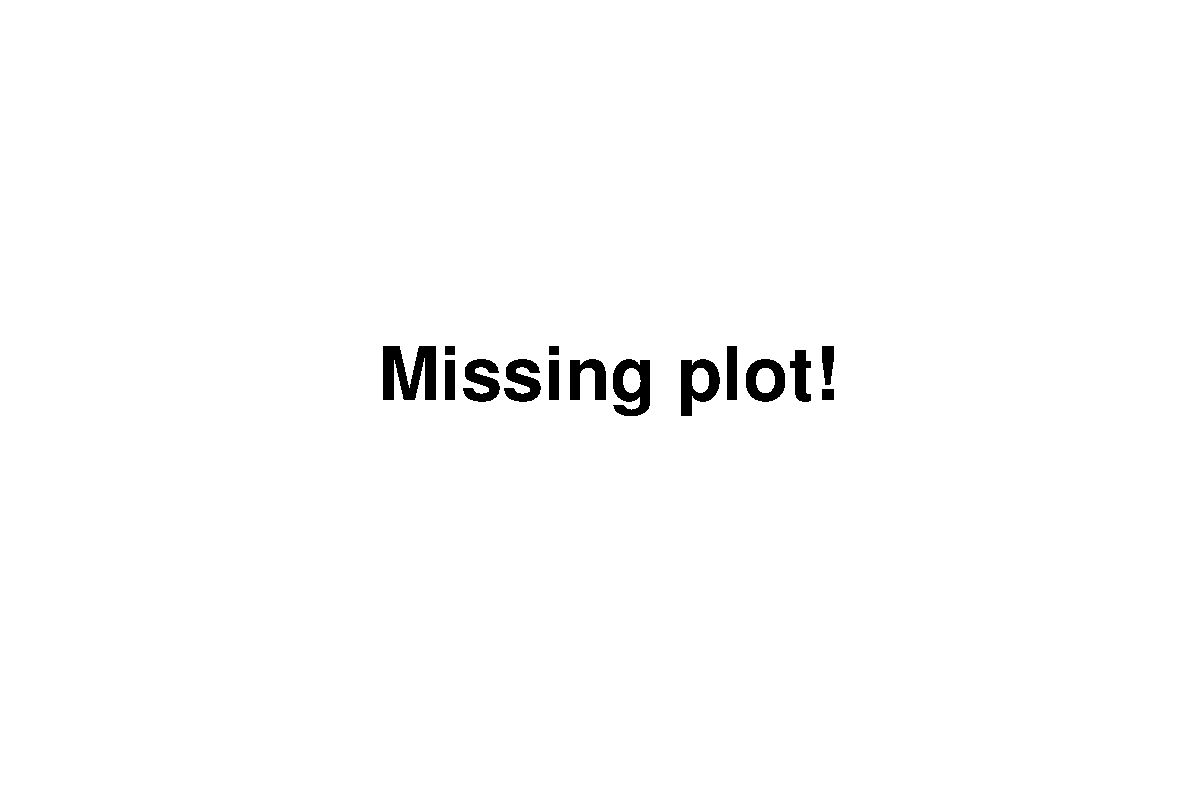
\includegraphics[width=0.9\textwidth]{./images/missing_plot-eps-converted-to.pdf}
%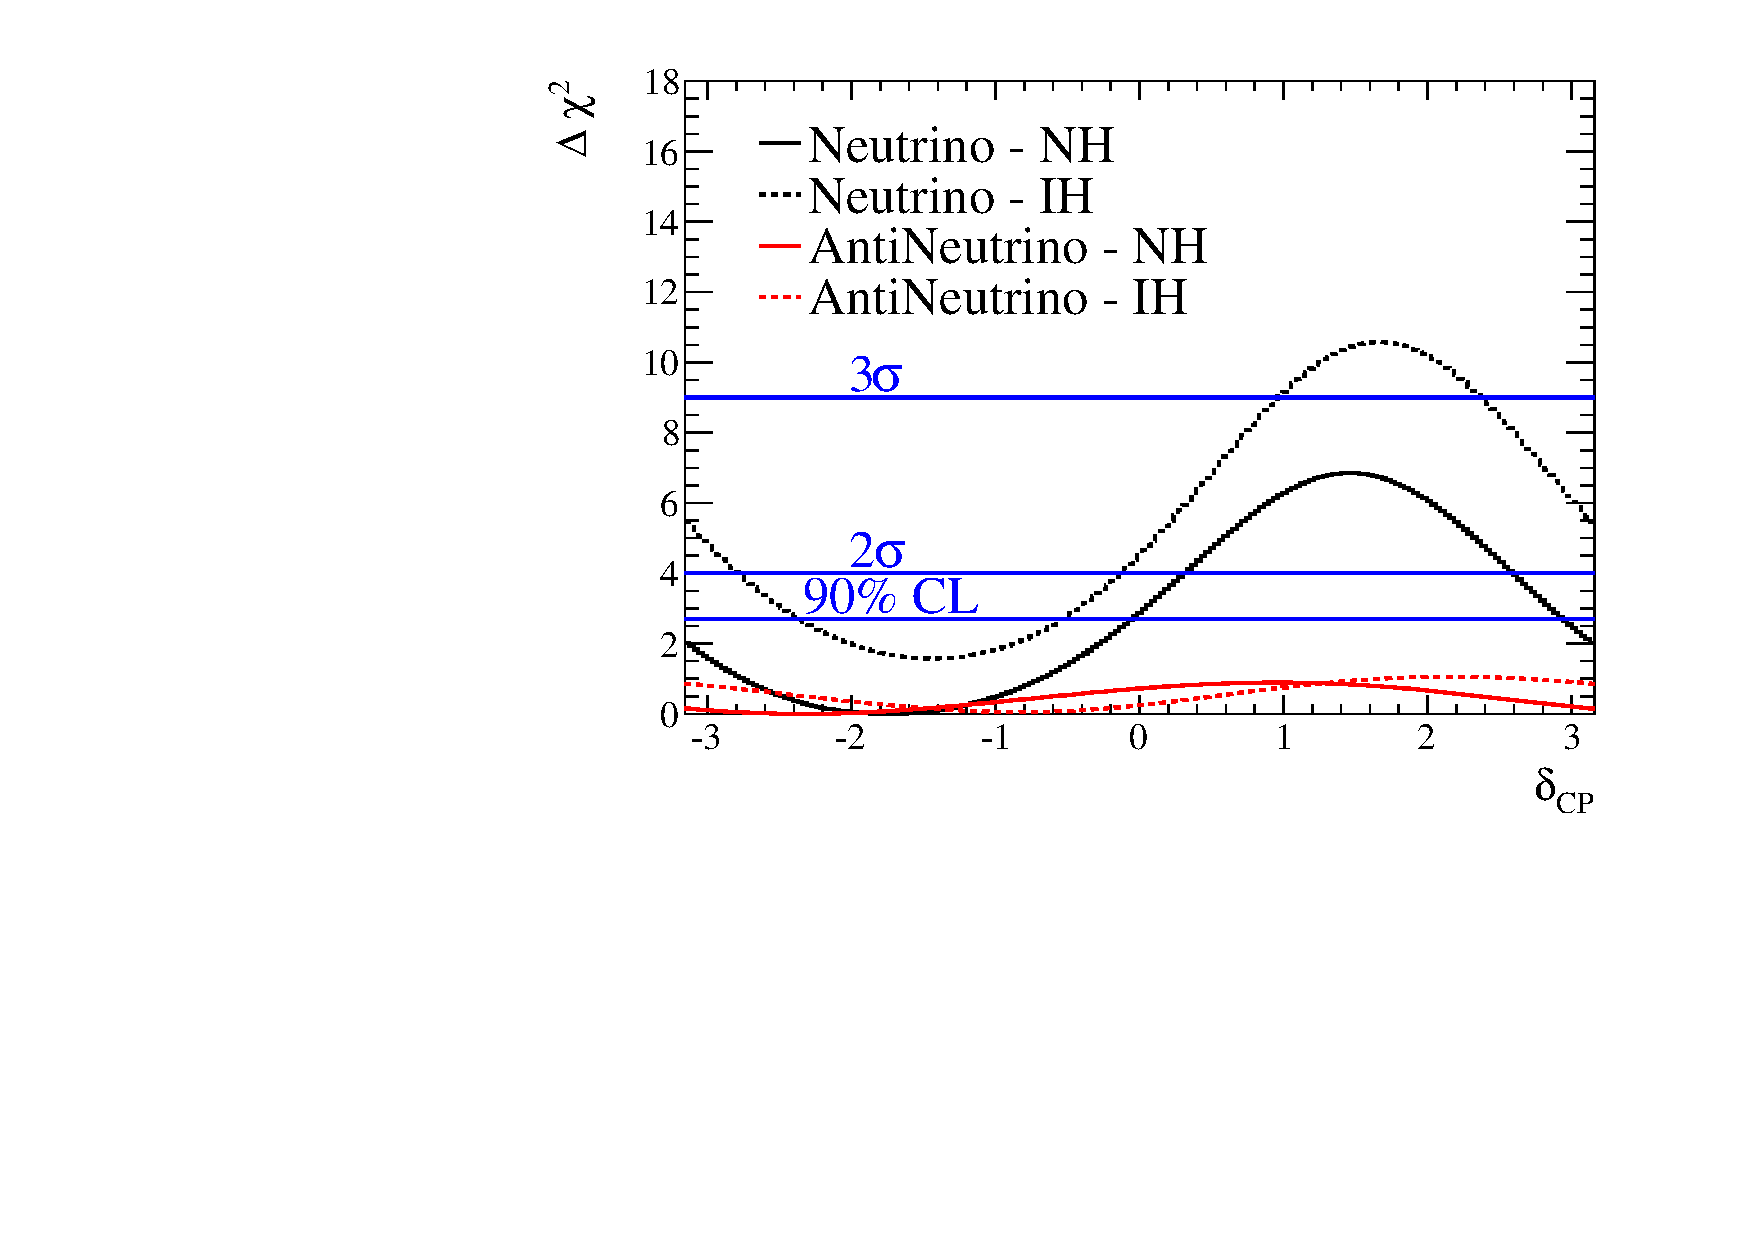
\includegraphics[width=0.5\textwidth]{./joint_plots/data_contours/dcp_react_data_constdchisq_fhcVsrhc.pdf}
%\caption{
%Measured $\Delta \chi^2$ distributions
%with the full Run 1-6 data set
%as a function of
%$\delta_{CP}$ 
%with reactor constraint
%independently for only neutrino and antineutrino mode data.
%Both normal (black) and inverted (red) hierarchies are shown. 
%%Both 68\% (dashed line) and 90\% CL (solid line) are shown.
%%For $\delta_{CP}$ confidence intervals are performed using the
%%\emph{Feldman-Cousins} method,
%%while for the other oscillation parameters
%The \emph{constant} $\Delta \chi^2$ method is used. %(see \cref{app:method_cl}).
%Both normal and inverted hierarchy $\Delta \chi^2$ distributions are shifted with respect to the same global minimum,
%independently for the neutrino and antineutrino mode data. 
%All the oscillation parameters which are not parameters of interest
%are marginalised using the prior distributions shown in \cref{tab:marg_binnning}.
%}
%\label{fig:joint_dcp_nu_nubar}
%\end{figure*}


%
% Rate-only analysis
%
%In \cref{fig:joint_data_fit_1d_rateonly} the $\chi^2$ distributions as a function of $\delta_{CP}$
%is obtained by performing a rate-only analysis; 
%instead of using the shape information of the $E_{reco}$ vs $\theta_l$ spectra,
%the total number of events of each sample is fitted, 
%reducing the $E_{reco}$ vs $\theta_l$ template to 1 bin.
%Then the best-fit value of $\delta_{CP}$ is -1.602 closer to $-\pi/2$ with respect to the case
%where the shape information is used.
%
%\begin{figure*}[htb]
%\center
%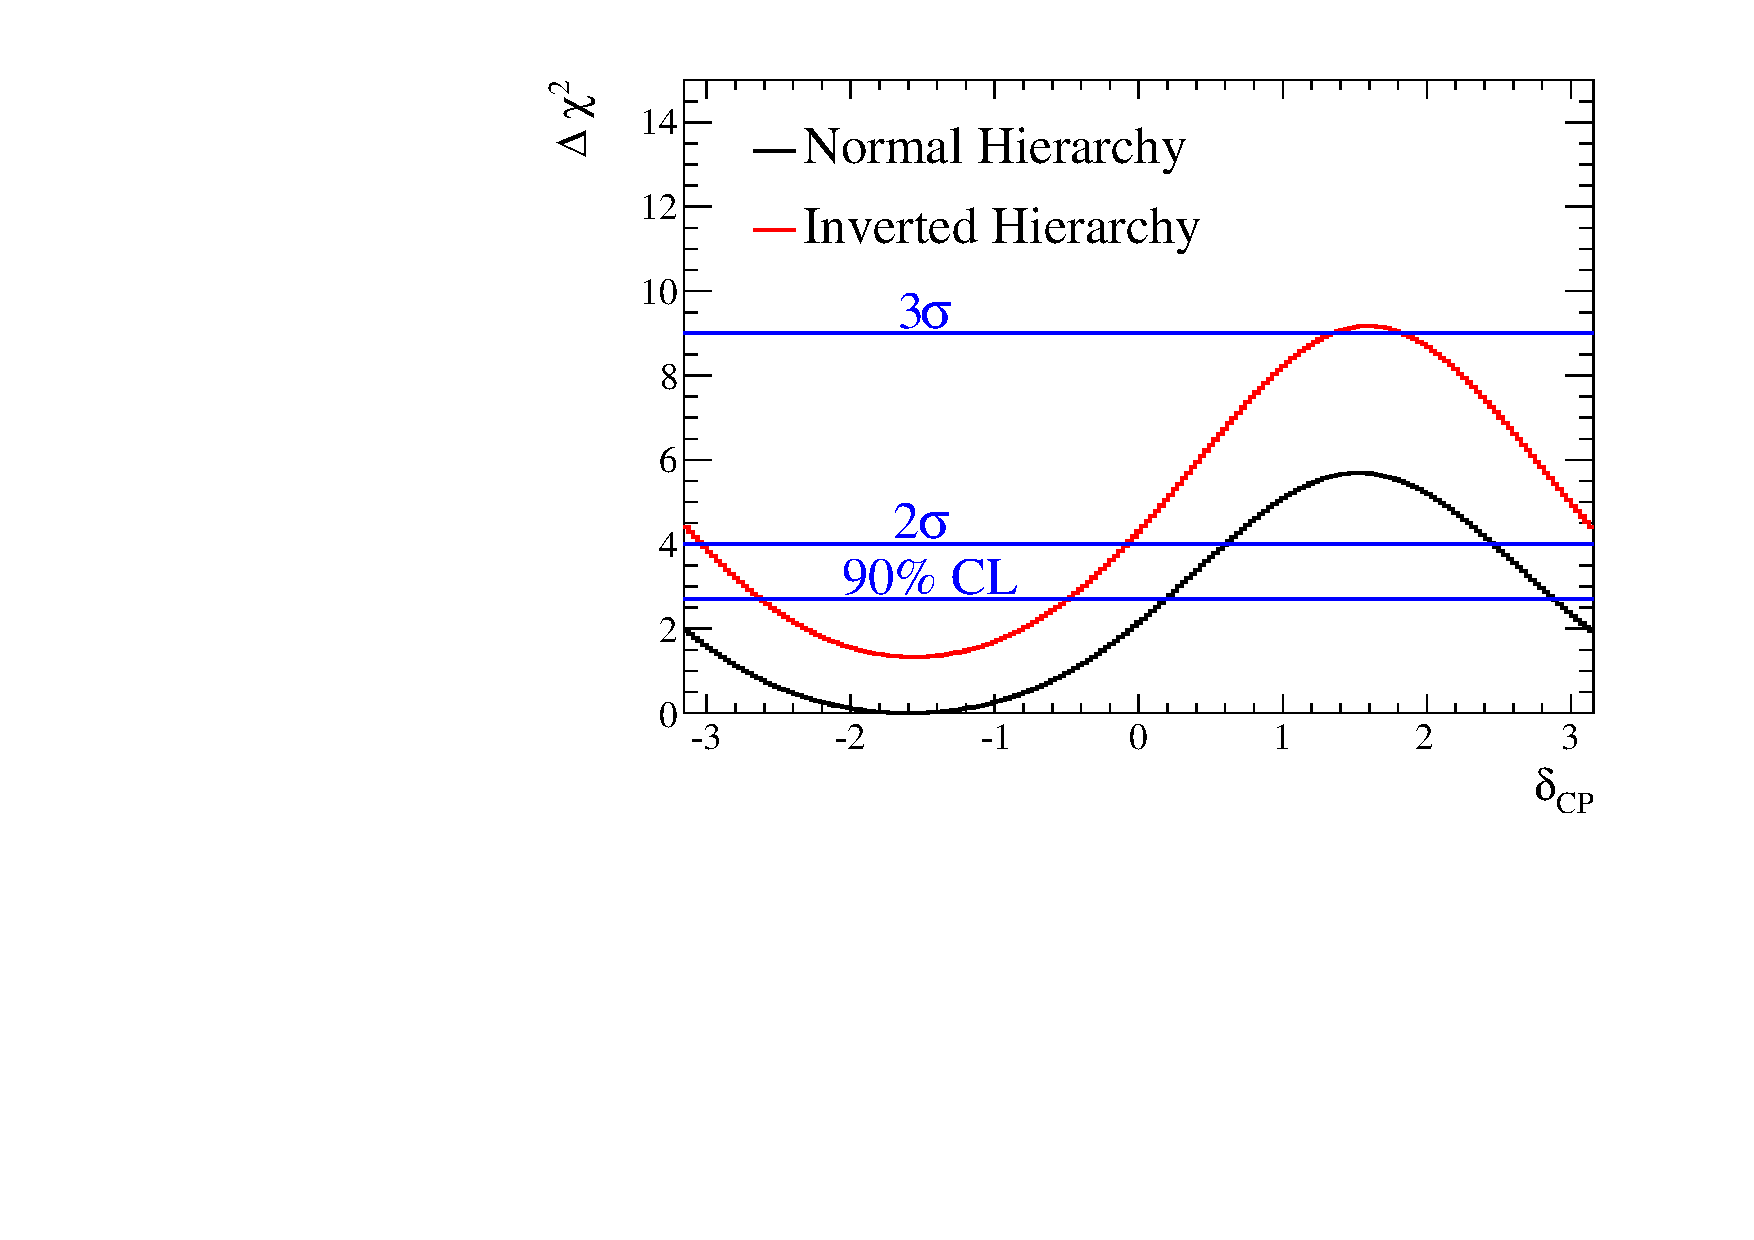
\includegraphics[width=0.5\textwidth]{joint_plots/data_contours/dcp_react_data_constdchisq_rateonly.pdf}
%\caption{
%Measured $\Delta \chi^2$ distributions
%with a rate-only analysis
%using the full Run 1-6 data set
%as a function of
%$\delta_{CP}$ 
%with reactor constraint.
%Both normal (black) and inverted (red) hierarchies are shown. 
%%Both 68\% (dashed line) and 90\% CL (solid line) are shown.
%%For $\delta_{CP}$ confidence intervals are performed using the
%The \emph{constant} $\Delta \chi^2$ method is used. %(see \cref{app:method_cl}).
%Both normal and inverted hierarchy $\Delta \chi^2$ distributions are shifted with respect to the same global minimum. 
%All the oscillation parameters which are not parameters of interest
%are marginalised using the prior distributions shown in \cref{tab:marg_binnning}.
%}
%\label{fig:joint_data_fit_1d_rateonly}
%\end{figure*}




% Table of best-fit and 1sigma ranges

In \cref{tab:joint_bestfit_run17c} the best-fit values as well as the $1\sigma$ ranges for each 
oscillation parameter are shown for the Run 1-7c data fit, for both normal and inverted hierarchy.
The $1\sigma$ ranges are extracted for each oscillation parameter
from the 1-dimensional $\Delta \chi^2$ distributions shown in \cref{fig:joint_data_fit_1d_run17c},
where one oscillation parameter is free and all the other oscillation as well as the systematic 
parameters are marginalised.
The mass hierarchy is minimized:
for both normal and inverted hierarchy the $1\sigma$ ranges are calculated with respect to the 
same global minimum.
Since this approach is not entirely correct and there does not exist any procedure 
to set more reliable confidence intervals which does not consist of toy MC studies (see \cref{sec:cl_mh}),
the advice to the reader is to give more importance to the difference in $\chi^2_{marg}$
between normal and inverted hierarchies in the respective best-fit points, 
instead of the $1\sigma$ ranges of inverted hierarchy, 
which are smaller by construction.
It is also worth to notice that the $1\sigma$ ranges for normal hierarchy (best-fit)
are set correctly with the constant $\Delta \chi^2$ method in the gaussian approximation.

%As already written above, the Run 1-7c best-fit value of $\delta_{CP}$ with reactor constraint is 
%close to the Run 1-6 one (see \cref{tab:joint_bestfit}).
%However if the reactor constraint is not applied, the Run 1-7c best-fit value of $\delta_{CP}$
%is quite different with respect to the Run 1-6 one:
%the best-fit for both normal and inverted hierarchy gets closer to $-\pi/2$.
%Indeed, as shown in \cref{fig:joint_data_fit_1d_run17c}, 
%the $\Delta \chi^2$ distribution as a function of $\delta_{CP}$ and mass hierarchy
%with T2K only data becomes more similar to the one obtained with the reactor constraint:
%assuming the constant $\Delta \chi^2$ method, $\delta_{CP}=0$ for normal hierarchy
%is excluded at 90\%CL and the maximal $\Delta \chi^2$ value is 
%larger than 4.5 and 8.5 respectively for normal and inverted hierarchy.
%The exclusion is stronger than the one given by the Run 1-6 where
%almost the full range $\delta_{CP}$ and normal hierarchy was allowed at 90\%CL.
%This is due to the downward fluctuation in the antineutrino mode $e$-like sample
%combined with an upward fluctuation in the neutrino mode $e$-like sample.
%Assuming Asimov data set A but with $\delta_{CP} = 0$ we expect 6.9
%antineutrino mode $e$-like events and 22.7 neutrino mode $e$-like events.
%If we assume $\delta_{CP}=-1.601$ we expect 26.9 and 6.0 events 
%for neutrino and antineutrino mode $e$-like samples.
%However we observe only 4 events in antineutrino mode and 
%32 events in neutrino mode $e$-like samples.
%Consequently the Run 1-7c data favor a smaller value of $\sin^2 \theta_{13}$,
%in better agreement with the reactor measurement,
%enhancing the tension due to the excess in the neutrino mode $e$-like sample.


%It is interesting to notice that the Run 1-7c $\pm 1\sigma$ interval of $\sin^2 \theta_{23}$ is slightly larger
%than the Run 1-6 one though the number of events in antineutrino mode $\mu$-like samples is almost double. 
%This can be qualitatively understood by comparing the observed and expected number of events
%in \cref{tab:num_events_run17c} (Run 1-7c) and~\ref{tab:num_events} (Run 1-6).
%In Run 1-6 data set the observed number of $\bar{\nu}_{\mu}$ candidates is 34, in good agreement
%with Asimov data set A, i.e. maximal disappearance, while in Run 1-7c data set we observe 66 events
%which is closer to the Asimov data set B, i.e. lower octant ($\sin^2 \theta_{23} = 0.45$).

All the confidence intervals are very similar to those from the 1Ring sample analysis.

\begin{table}[htb]
\centering
\begin{tabular}{| c | c || c | c | c || c | c | c |}
\hline
								& {\bf Reactors}		& \multicolumn{3}{c||}{\bf Normal Hierarchy} & \multicolumn{3}{c|}{\bf Inverted Hierarchy} \\
\hline										
\bf Parameter						&				& Best-fit	& $\chi^2_{min}$	& $\pm 1\sigma$ 	  	 	& Best-fit		& $\chi^2_{min}$ 	& $\pm 1\sigma$ global (inverted) 	 \\
\hline
$\delta_{CP}$             				& YES      			& -1.728  	& 370.61			& [-2.538; -0.877]			& -1.445		& 373.07			& -							\\
								& 				& 		& 				& 						& 			& 				& ([-2.170; -0.768])				\\ 
\hline
$\delta_{CP}$            				& NO        			& -1.791  	& 373.53			& [-2.789; -0.764]			& -1.382		& 375.17			& -							\\
								& 				& 		& 				& 						& 			& 				& ([-2.296;-0.524]) 				\\ 
\hline
$\sin^2 \theta_{13}$    				& NO             		& 0.0271 & 371.44			& [0.0209; 0.0342]			& 0.0299		& 373.38			& -							\\
								& 				& 		& 				& 						& 			& 				& ([0.0232; 0.0380]) 				\\ 
\hline
$\sin^2 \theta_{23}$                      		& YES       		& 0.550	& 369.80			& [0.465; 0.601]			& 0.5525		& 372.30			& -                 					\\
								& 				& 		& 				& 						& 			& 				& ([0.470; 0.601])			  	\\ 
\hline
$\Delta m^2_{32}$ or $\Delta m^2_{13}$   & YES  			& 2.54 	& 369.05	 		& [2.460; 2.621]			& 2.51 		& 297.56			& -     						\\
%								& 				& 		& 				& 						& 			& 				& 				 \\ 
%\hline
($10^{-3} ~\text{eV}^2 / c^4$) 			& 				& 		&				&						&			&				& ([2.429; 2.588])							\\
%								& 				& 		& 				& 						& 			& 				&							 \\ 

\hline
\end{tabular}
\caption{
The Run 1-7c measured oscillation parameter best-fit
and minimum $\chi^2$ 
values  
as well as the 
$1\sigma$ 
CL intervals are shown,
for both normal and inverted hierarchy. 
The $\pm1\sigma$ interval is obtained by using the 
\emph{constant} $\Delta \chi^2$ method.
All the parameters are measured using the reactor constraint 
$\sin^2 2\theta_{13} = 0.085 \pm 0.005 $
\cite{pdg_2014},
except for $\delta_{CP}$ and $\sin^2 \theta_{13}$.
For the inverted hierarchy the intervals are calculated both with respect to 
the global minimum, i.e. normal hierarchy, as well as 
independently for inverted hierarchy (between parenthesis in second row).
As explained in \cref{sec:cl_mh}, the gaussian approximation does not work well 
for discrete parameters like the mass hierarchy however, since there is not a clear way
to compute $1\sigma$ ranges for both mass hierarchies without performing
CPU intensive toy MC studies, the constant $\Delta \chi^2$ method is used.
}                                                                                                                                                                                          
\label{tab:joint_bestfit_run17c}
\end{table}






% Best-fit spectra
{\huge{TO UPDATE}}

The best-fit spectra, shown in \cref{fig:joint_spectra_bf_run17c} are computed as described in \cref{sec:spectra_bestfit_method}
and are compared to the unoscillated nominal spectra.
For $e$-like samples, where 2-dimensional templates are used,
the projection onto the reconstructed neutrino energy axis is shown.
All the systematic and oscillation parameters are marginalised following the procedure described in \cref{sec:spectra_bestfit_method},
while $\sin^2\theta_{23}$, $\delta_{CP}$ and the mass hierarchy were fixed to their best-fit values 
obtained from their simultaneous fit, i.e. \cref{fig:ss23_dcp_with_reactor_data_fit_run17c}.
Indeed these oscillation parameters have the strongest effect on the measurement,
since $\sin^2\theta_{13}$ is constrained with the reactor measurement.

\begin{figure*}[htb]
\center
\begin{subfigure}[b]{0.49\textwidth}
%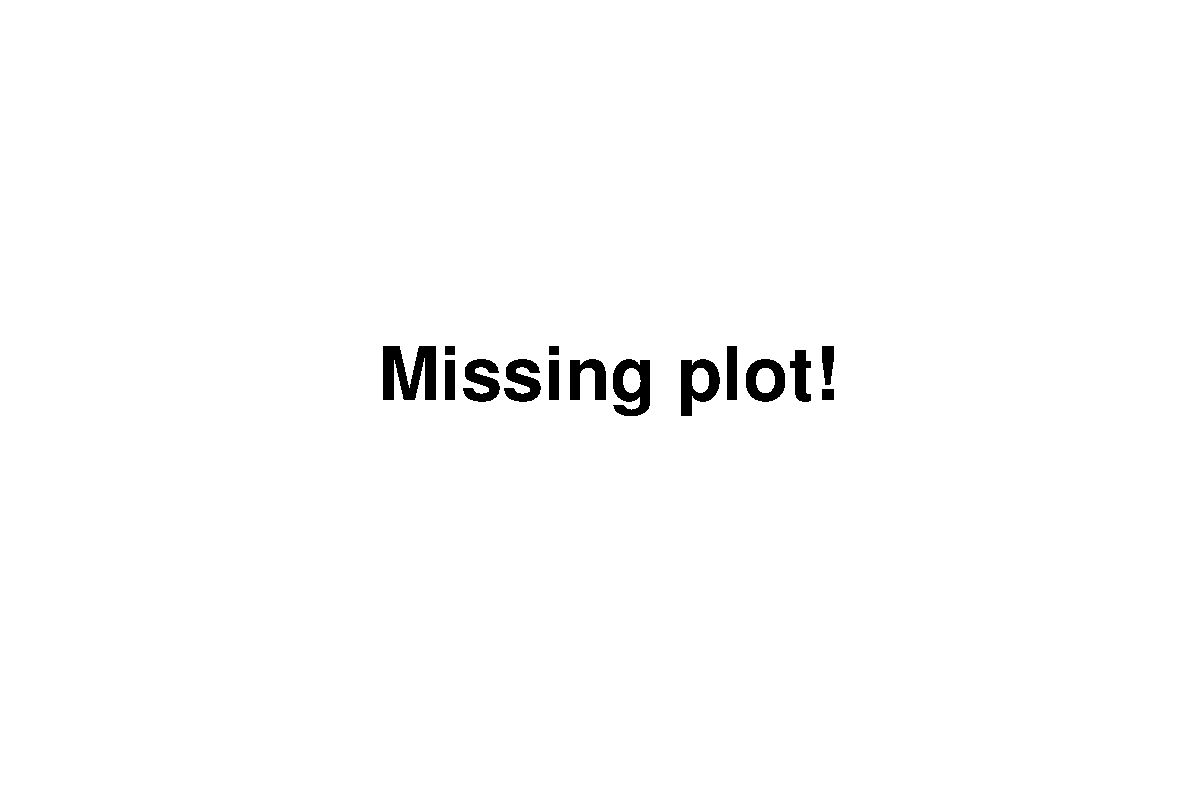
\includegraphics[width=0.9\textwidth]{./images/missing_plot-eps-converted-to.pdf}
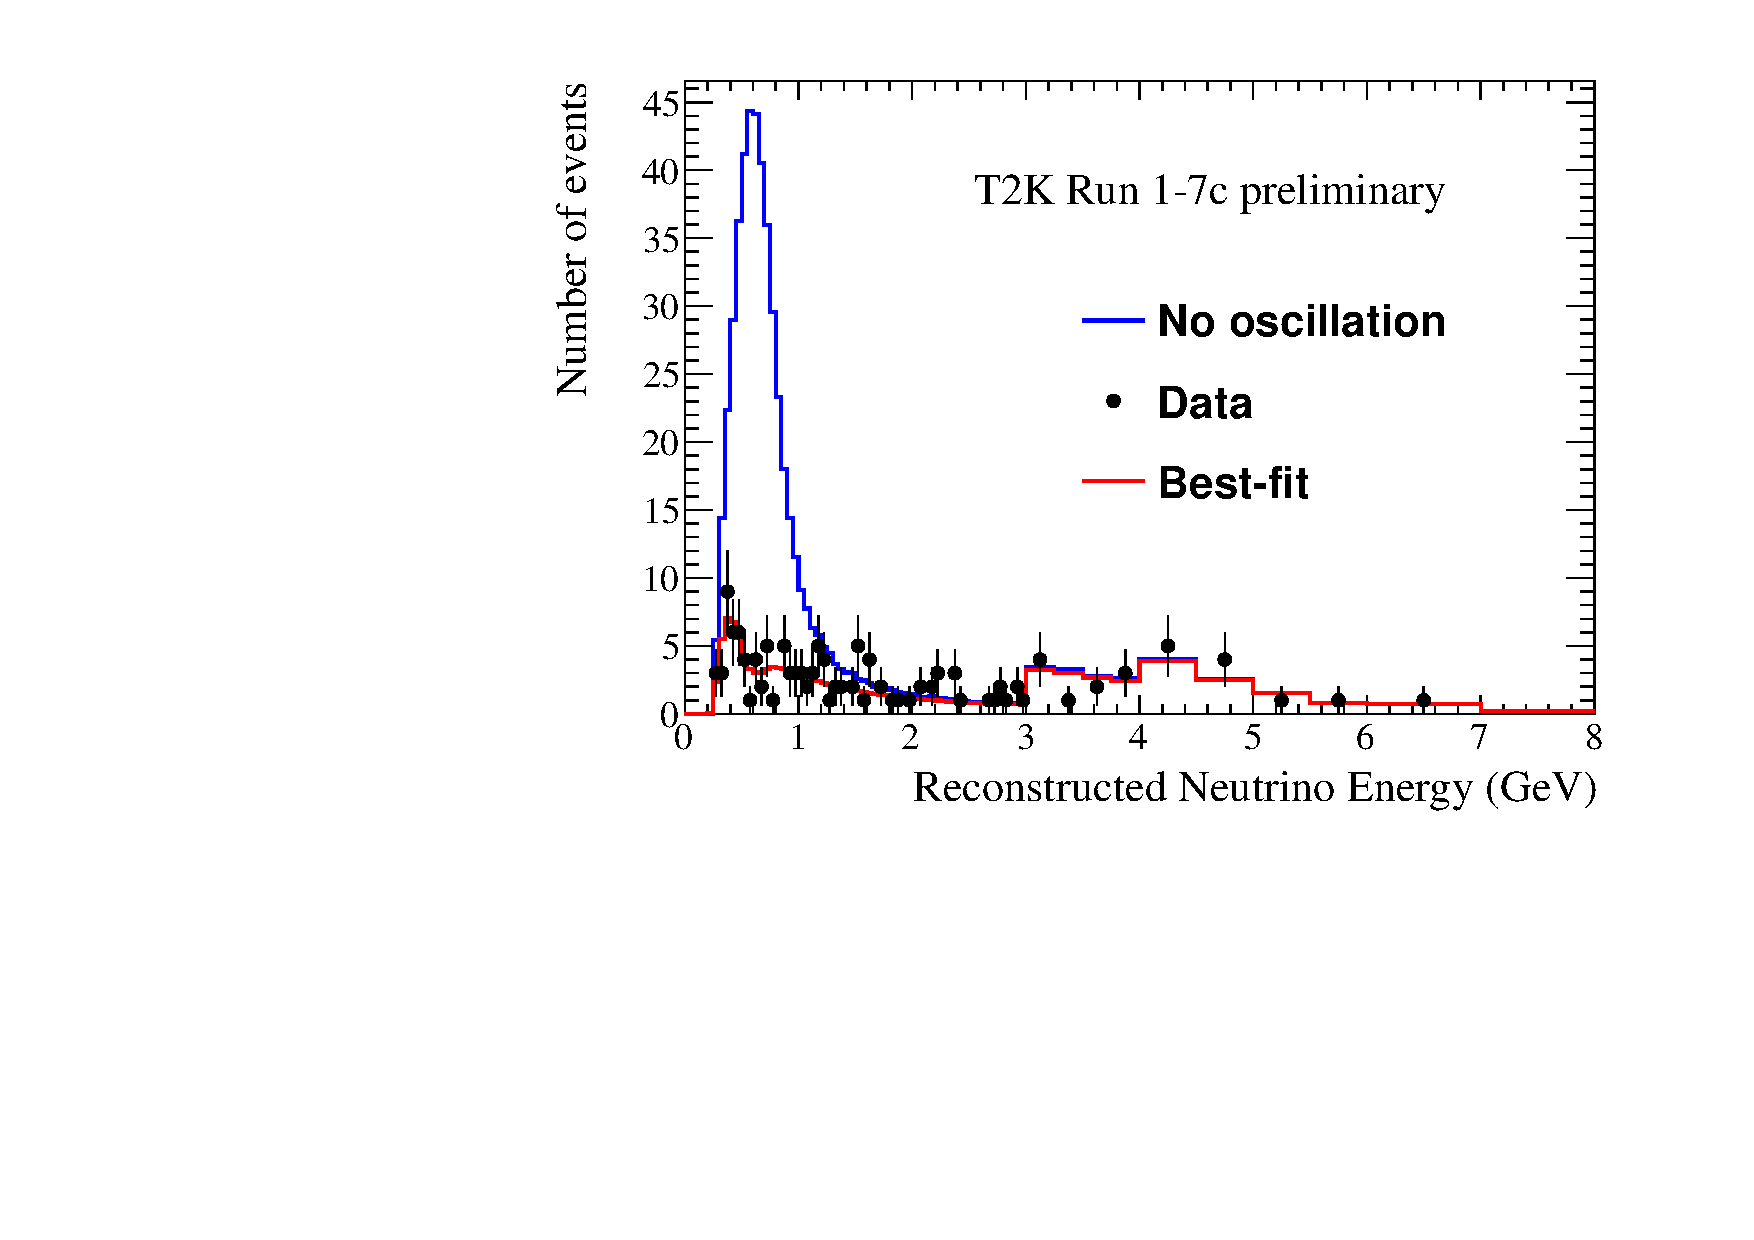
\includegraphics[width=0.9\textwidth]{joint_plots/data/Run17c/bestfit_sinsqth23VsdcpVsMH_1Rmu_Run17.pdf}
\caption{Muon-like, neutrino mode}
\end{subfigure}
\begin{subfigure}[b]{0.49\textwidth}
%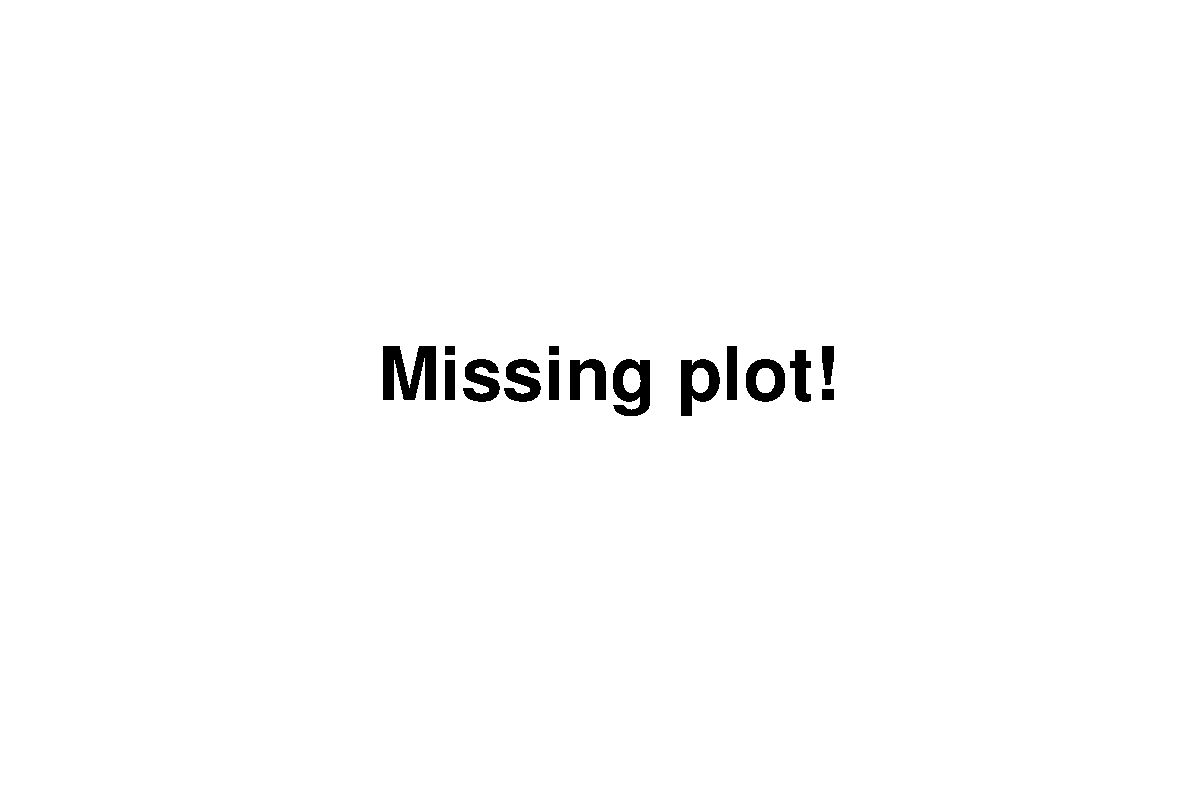
\includegraphics[width=0.9\textwidth]{./images/missing_plot-eps-converted-to.pdf}
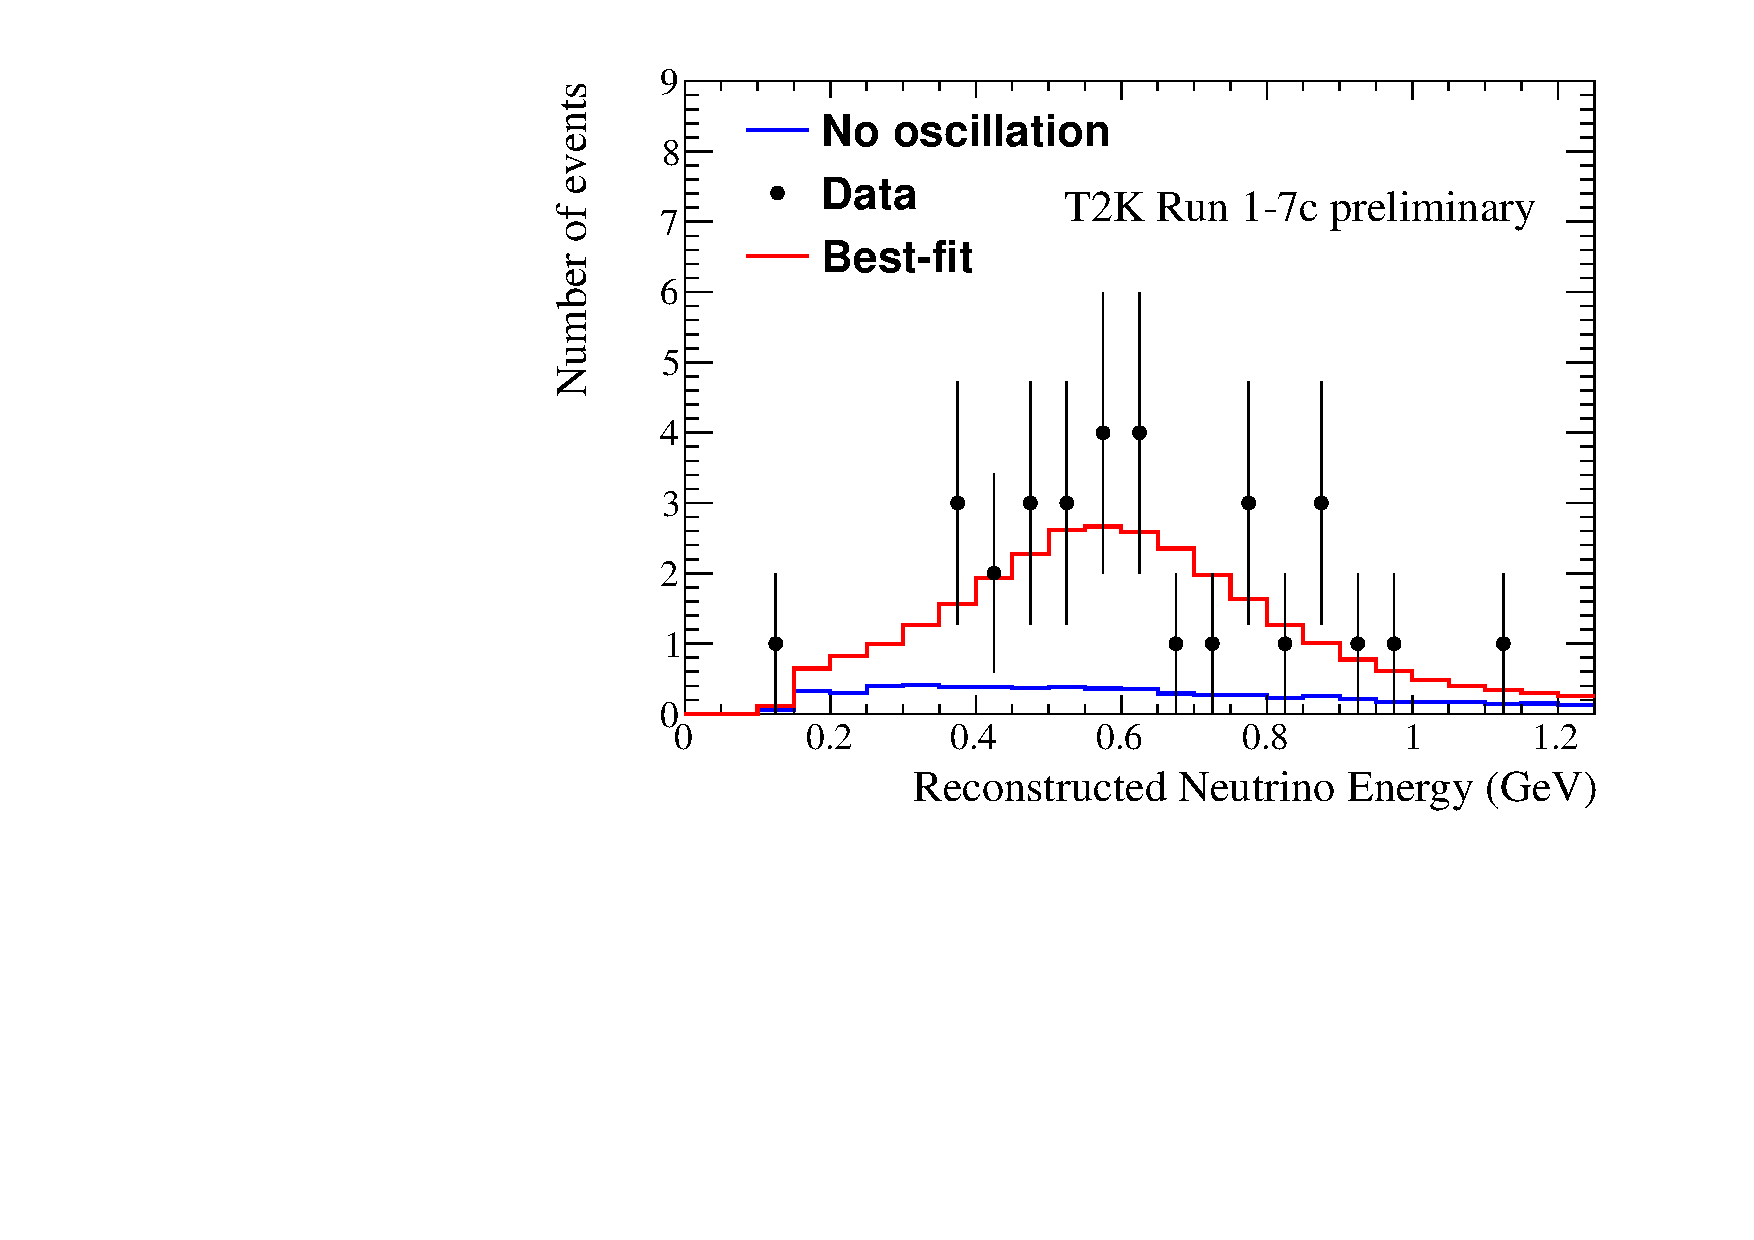
\includegraphics[width=0.9\textwidth]{joint_plots/data/Run17c/bestfit_sinsqth23VsdcpVsMH_1Re_Run17.pdf}
\caption{Electron-like, neutrino mode}
\end{subfigure}
\begin{subfigure}[b]{0.49\textwidth}
%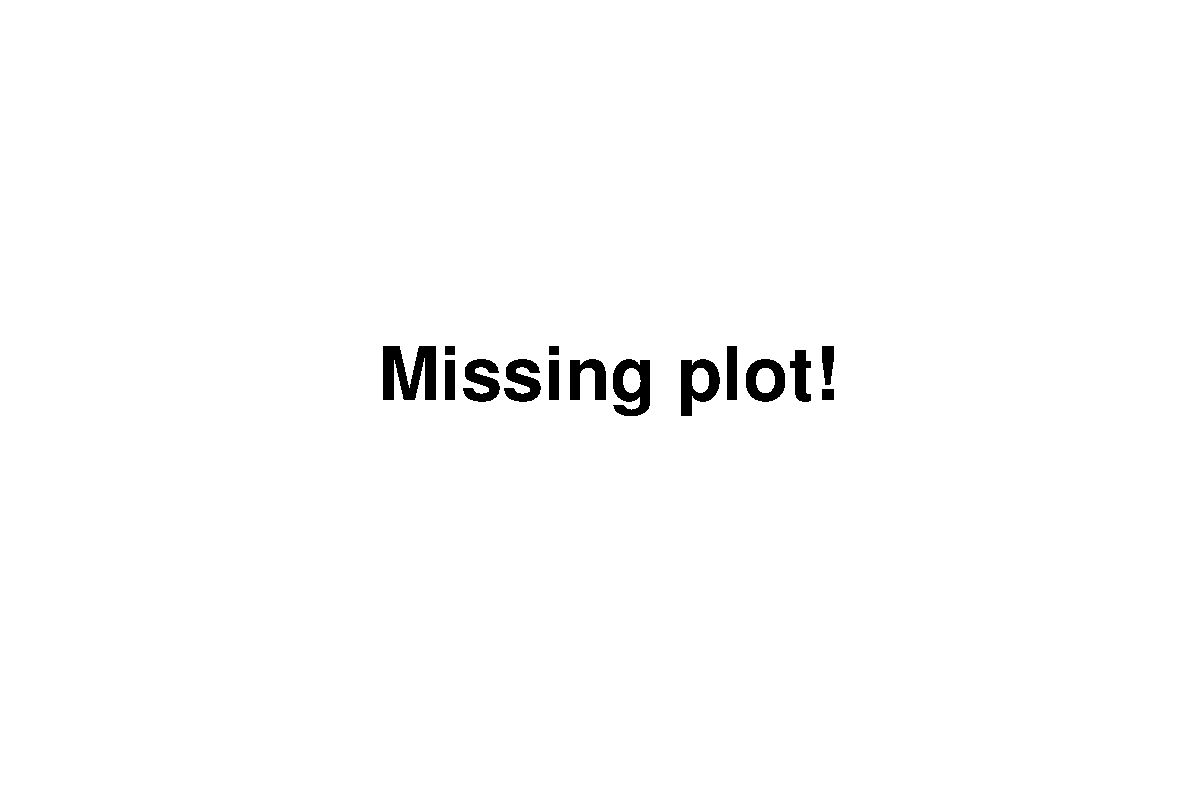
\includegraphics[width=0.9\textwidth]{./images/missing_plot-eps-converted-to.pdf}
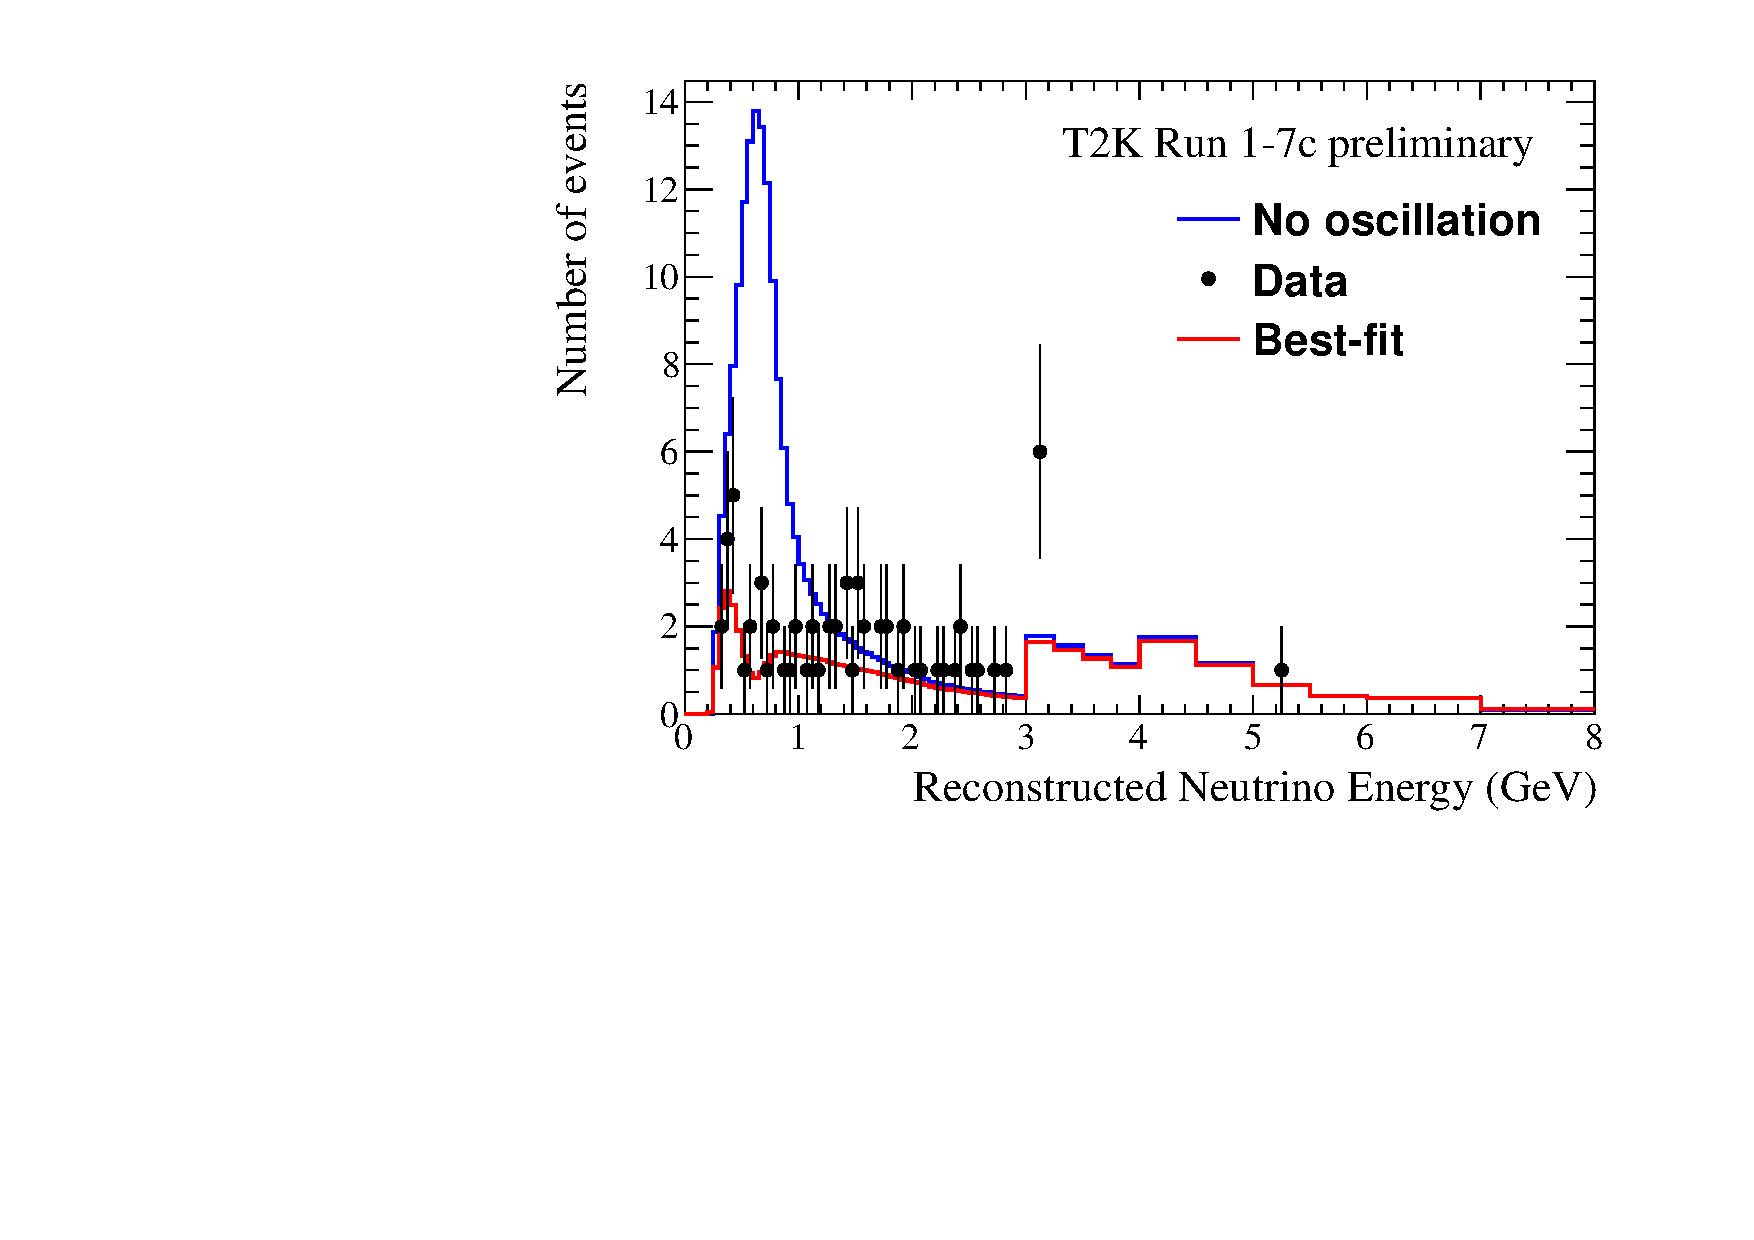
\includegraphics[width=0.9\textwidth]{joint_plots/data/Run17c/bestfit_sinsqth23VsdcpVsMH_RHC1Rmu_Run17.pdf}
\caption{Muon-like, antineutrino mode}
\end{subfigure}
\begin{subfigure}[b]{0.49\textwidth}
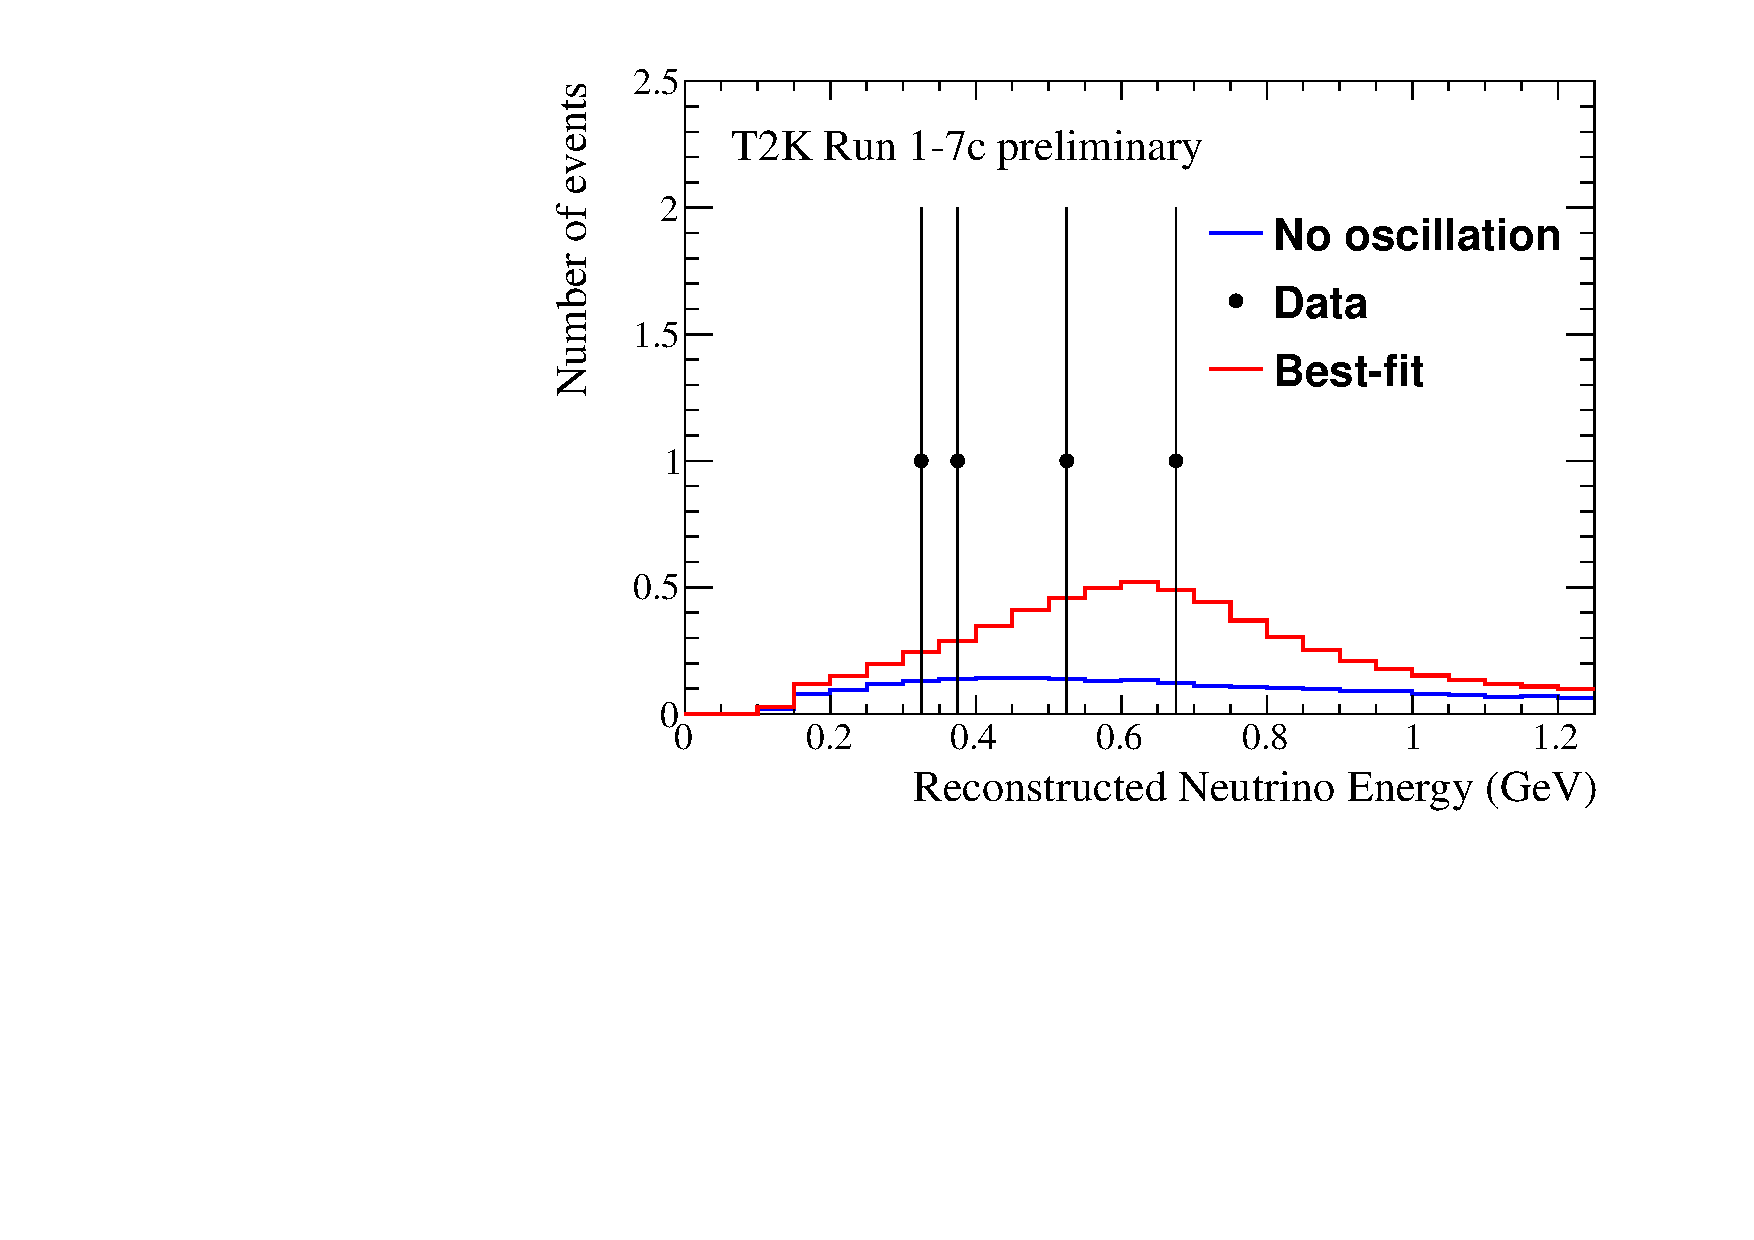
\includegraphics[width=0.9\textwidth]{joint_plots/data/Run17c/bestfit_sinsqth23VsdcpVsMH_RHC1Re_Run17.pdf}
%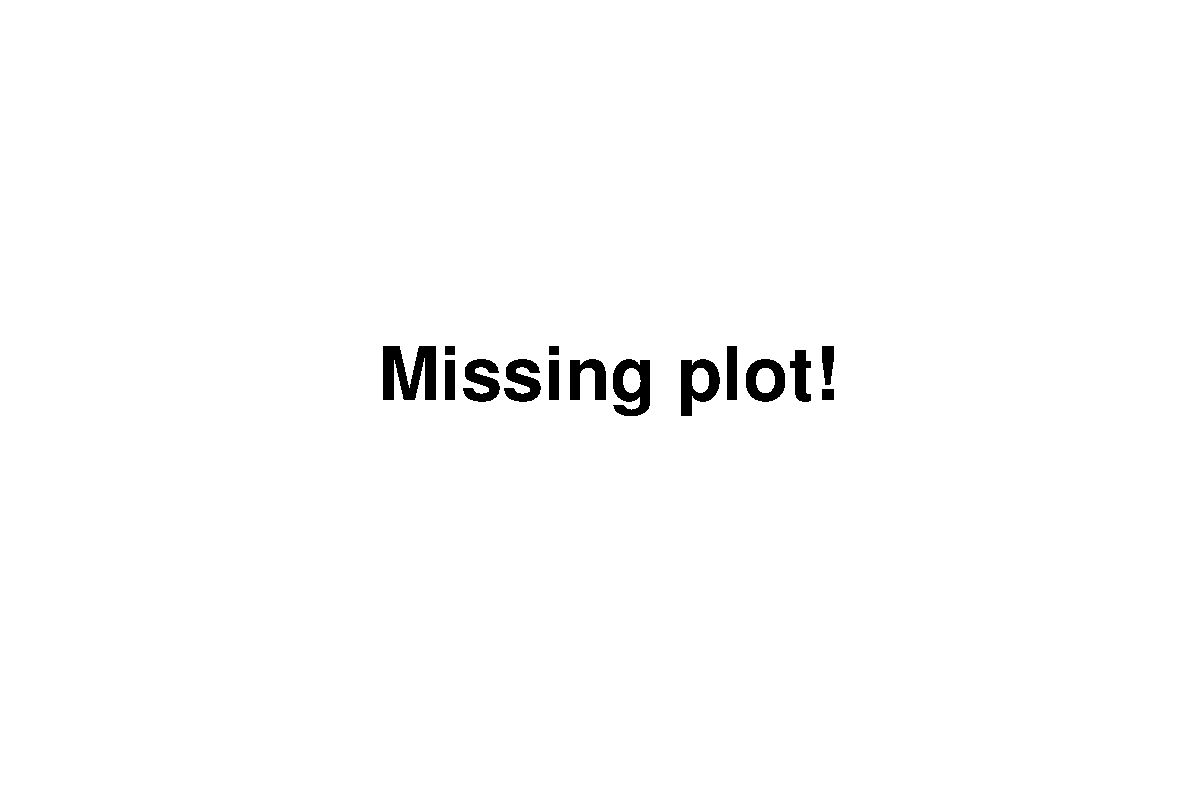
\includegraphics[width=0.9\textwidth]{./images/missing_plot-eps-converted-to.pdf}
\caption{Electron-like, antineutrino mode}
\end{subfigure}
\caption {
The best-fit spectra as a function of the neutrino reconstructed energy
are shown for each selected sample
of the Run 1-7c data set.
They correspond to the fit of 
$\sin^2 \theta_{23}$, $\delta_{CP}$ and mass hierarchy 
with reactor constraint
where all the nuisance parameters are marginalised. 
The method described in \cref{eq:bestfit_spectrum_marg} is used.
The best-fit distributions are compared with the 
predicted unoscillated spectrum (all the oscillation parameters are set to 0),
generated with the systematic parameters measured with the ND280 data 
shown in \cref{tab:banff_uncertainties_flux_fhc},
~\ref{tab:banff_uncertainties_flux_rhc},
~\ref{tab:banff_uncertainties_xsec}
and
the nominal Super-K systematic parameters shown in \cref{tab:banff_uncertainties_skdetfsi}.
}
\label{fig:joint_spectra_bf_run17c}
\end{figure*}







% Goodness of fit

A goodness of fit test is performed by comparing data with the best fit spectra shown in \cref{fig:joint_spectra_bf_run17c}.
The same method used for the Run 1-6 and Run 1-7b data sets, shown in \cref{sec:chisq_1d}, is used.
The goodness of fit test has been performed using the same binning as for Run 1-6,
i.e. 5 reconstructed neutrino energy bins (0-0.4, 0.4-0.7, 0.7-1.0, 1.0-2.0 and 2.0-30.0 GeV)
for neutrino mode $\mu$-like and 1 bin for all the other Super-K samples, 
as well as using 5 bins with the same binning as above for both the $\mu$-like samples,
since the antineutrino mode $\mu$-like sample has double of the statistic with Run 1-7c.
At least 6 events are present in each bin.

The $\chi^2$ and resulting p-value for each spectrum is shown in \cref{tab:goodness_of_fit_run17c}. 
We see for all the spectra, the data and best fit spectra are very compatible.

\begin{table}[htb]
\centering
\begin{tabular}{| c | c | c | c |}
\hline
\multicolumn{3}{| c |}{1 bin antineutrino mode $\mu$-like sample}  \\
\hline
Mass Hierarchy d.o.f. 			& $\chi^2$ / ndf        		& p-value \\ \hline
fixed					 		& 2.37348 / 6                  	& 0.88	\\ \hline
free					 		& 2.37348 / 5                 	& 0.80	\\ \hline
\hline
\multicolumn{3}{| c |}{5 bins antineutrino mode $\mu$-like sample}  \\
\hline
Mass Hierarchy d.o.f. 			& $\chi^2$ / ndf        		& p-value \\ \hline
fixed					 		& 3.80457 / 10                  	& 0.96	\\ \hline
free					 		& 3.80457 / 9                 	& 0.92	\\ \hline
\end{tabular}
\caption{
Goodness of fit for the Run 1-7c fit of $\sin^2 \theta_{23}$, $\delta_{CP}$ and mass hierarchy 
where all the other parameters are marginalised. 
Since the mass hierarchy is a discrete parameter, the goodness of the fit test 
is performed assuming the mass hierarchy both as a free parameter and as a fixed parameter.
$ndf = 5$ if the mass hierarchy is assumed to behave as 1 degree of freedom.
The test is performed with both 1 and 5 reconstructed neutrino energy bins for 
antineutrino mode $\mu$-like sample.
}
\label{tab:goodness_of_fit_run17c}
\end{table}



%%--------------------------------------------------------------------------------------
%%
%% Feldman-Cousins deltaCP Vs mh
%%
%%--------------------------------------------------------------------------------------
%
\subsection {Feldman-Cousins and significance for the simultaneous fit of $\delta_{CP}$ and mass hierarchy for Run 1-7c}
\label{sec:fc_significance_run17c}
{\huge{Update}}
%
%
%In \cref{fig:joint_dcp_fc_run17c} the confidence intervals obtained with the ``Feldman-Cousins" method
%are shown for $\delta_{CP}$ and mass hierarchy with reactor constraint for the Run 1-7c data set.
%The critical values at both 90\% and $2\sigma$ CL are computed
%for both the mass hierarchies and the following true values of $\delta_{CP}$: 
%$-\pi$, -2.356, $-\pi/2$, -0.785, 0, +0.785, $+\pi/2$, -2.356, $+\pi$. 
%The procedure described in \cref{sec:cl} is used.
%About 10k toy experiments were used for all the true points except $\delta_{CP} = \pi$ - normal hierarchy.
%Indeed the Run 1-7c data $\Delta \chi^2$ value is very close to the 90\% CL critical value, within one standard deviation of the critical value,
%if only 10k toy experiments are used. 
%For this reason, in order to provide a more precise statement about the 
%90\% CL exclusion of $\delta_{CP} = \pi$ - normal hierarchy, about 28k toy experiments are used, 
%so that the data $\Delta \chi^2$ value is outside the $\pm 1 \sigma$ critical value error.
%This can be seen in in \cref{fig:joint_dcp_fc_run17c}
%where the $\pm 1 \sigma$ error on the critical values are shown as well.
%The same procedure used for the Run 1-6 and Run 1-7b data fit, shown in \cref{sec:fc_significance}, is used.
%Inverted hierarchy is almost excluded at 90\% CL except for a small interval around $\delta_{CP} = -\pi / 2$.
%$\delta_{CP} = 0$ is still disfavored with respect to $\delta_{CP} = \pi$, which, however, is excluded at 90\% CL. 
%We can say that CP conservation assuming the PMNS framework is excluded at 90\% CL also for the Run 1-7c data set,
%though the p-value for $\delta_{CP} = \pi$ and normal hierarchy is very close to 0.1. 
%
%\begin{figure*}[htb]
%\center
%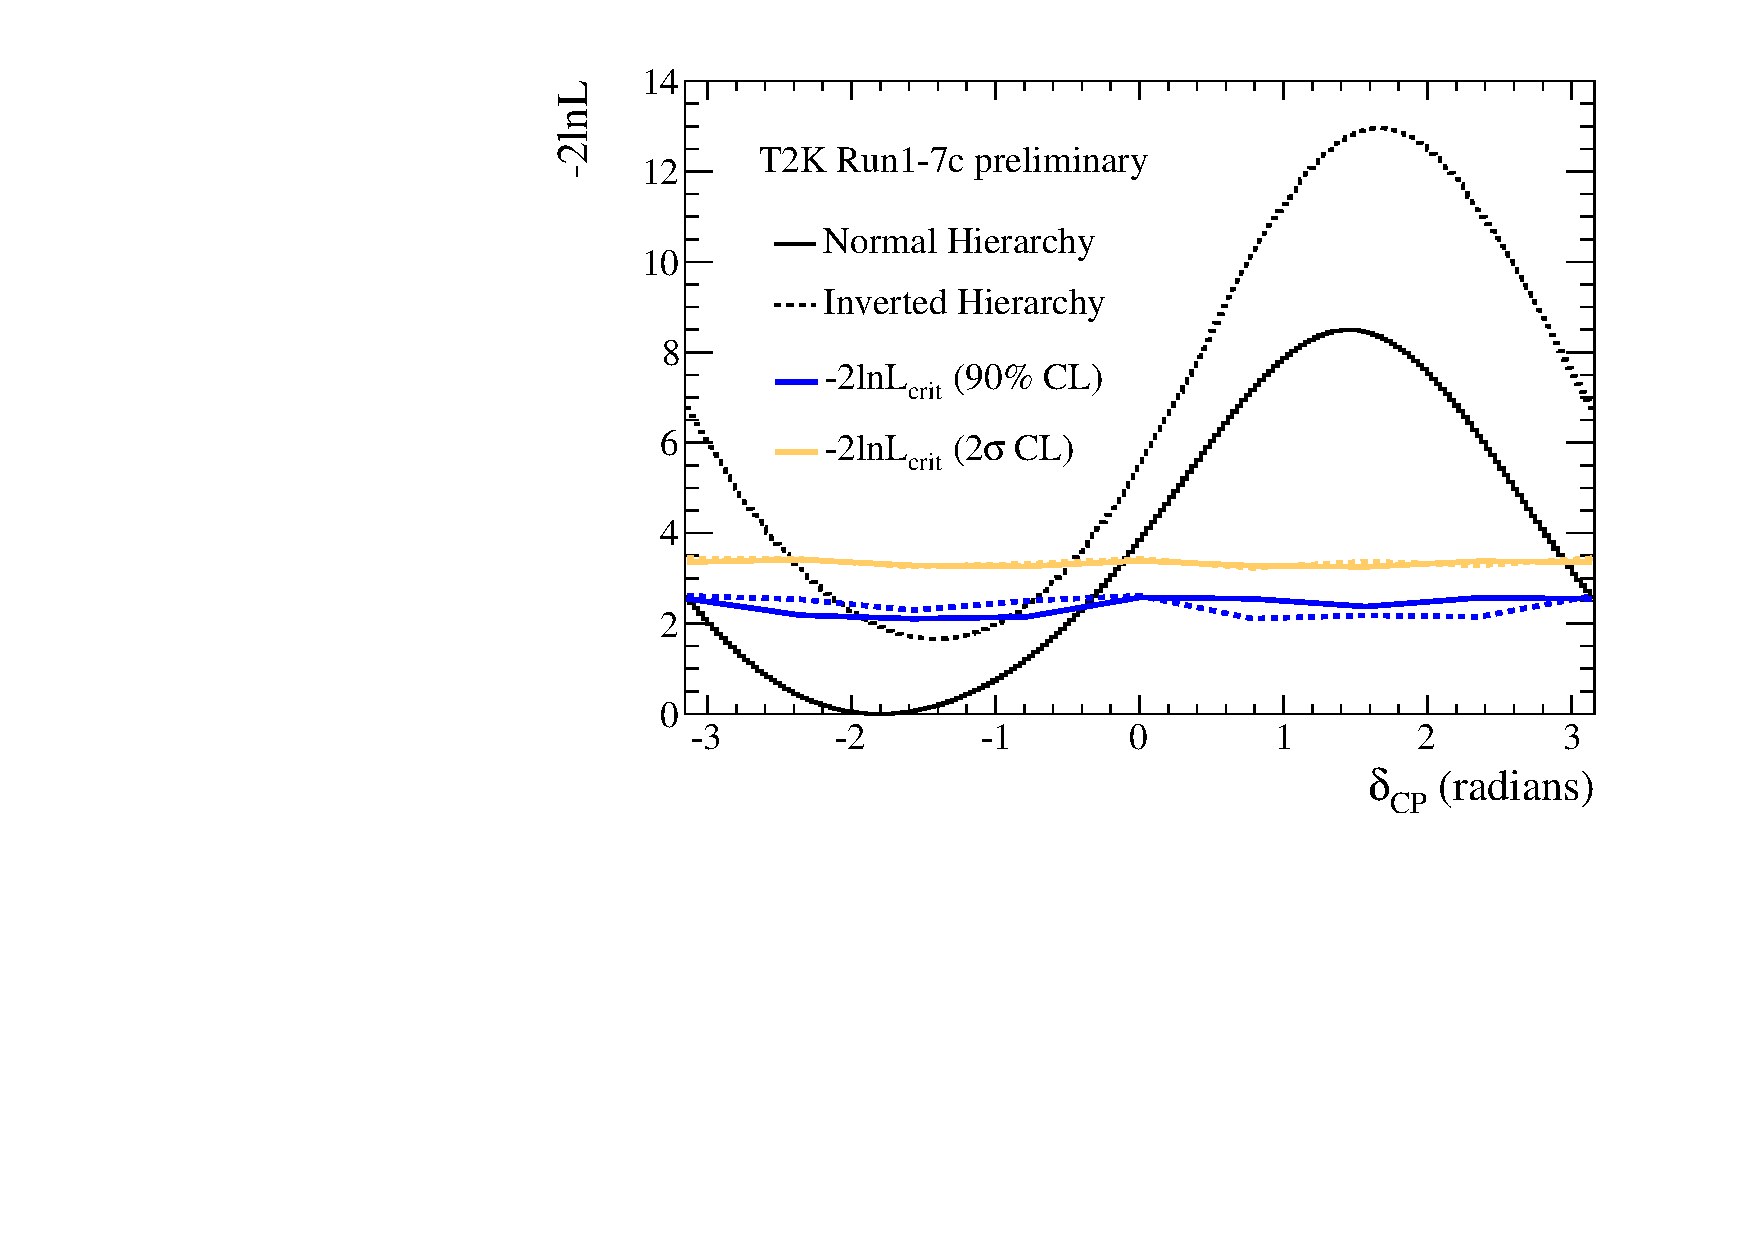
\includegraphics[width=0.49\textwidth]{joint_plots/coverage_fc/fc_run17c/dcp_mh_react_run17.pdf} 
%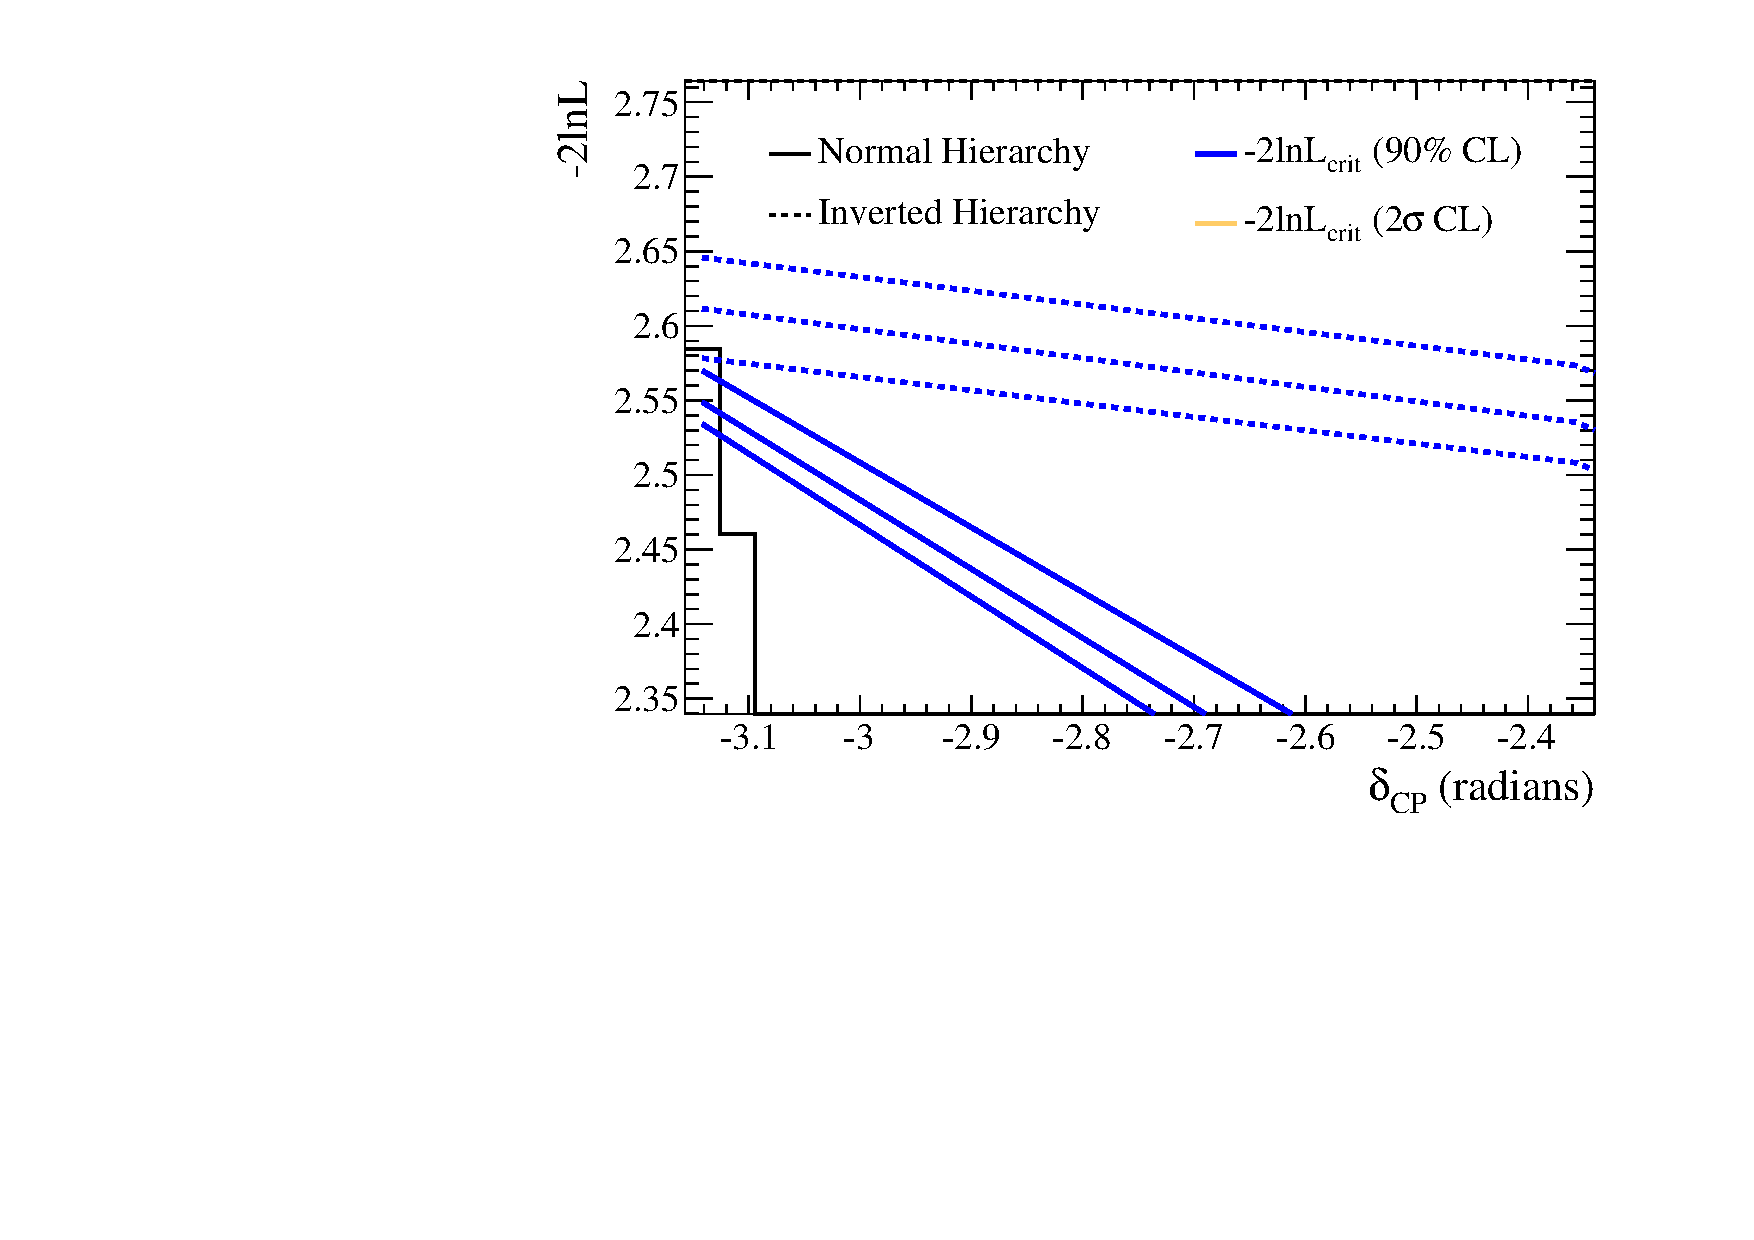
\includegraphics[width=0.49\textwidth]{joint_plots/coverage_fc/fc_run17c/dcp_mh_react_run17_zoom.pdf} \\
%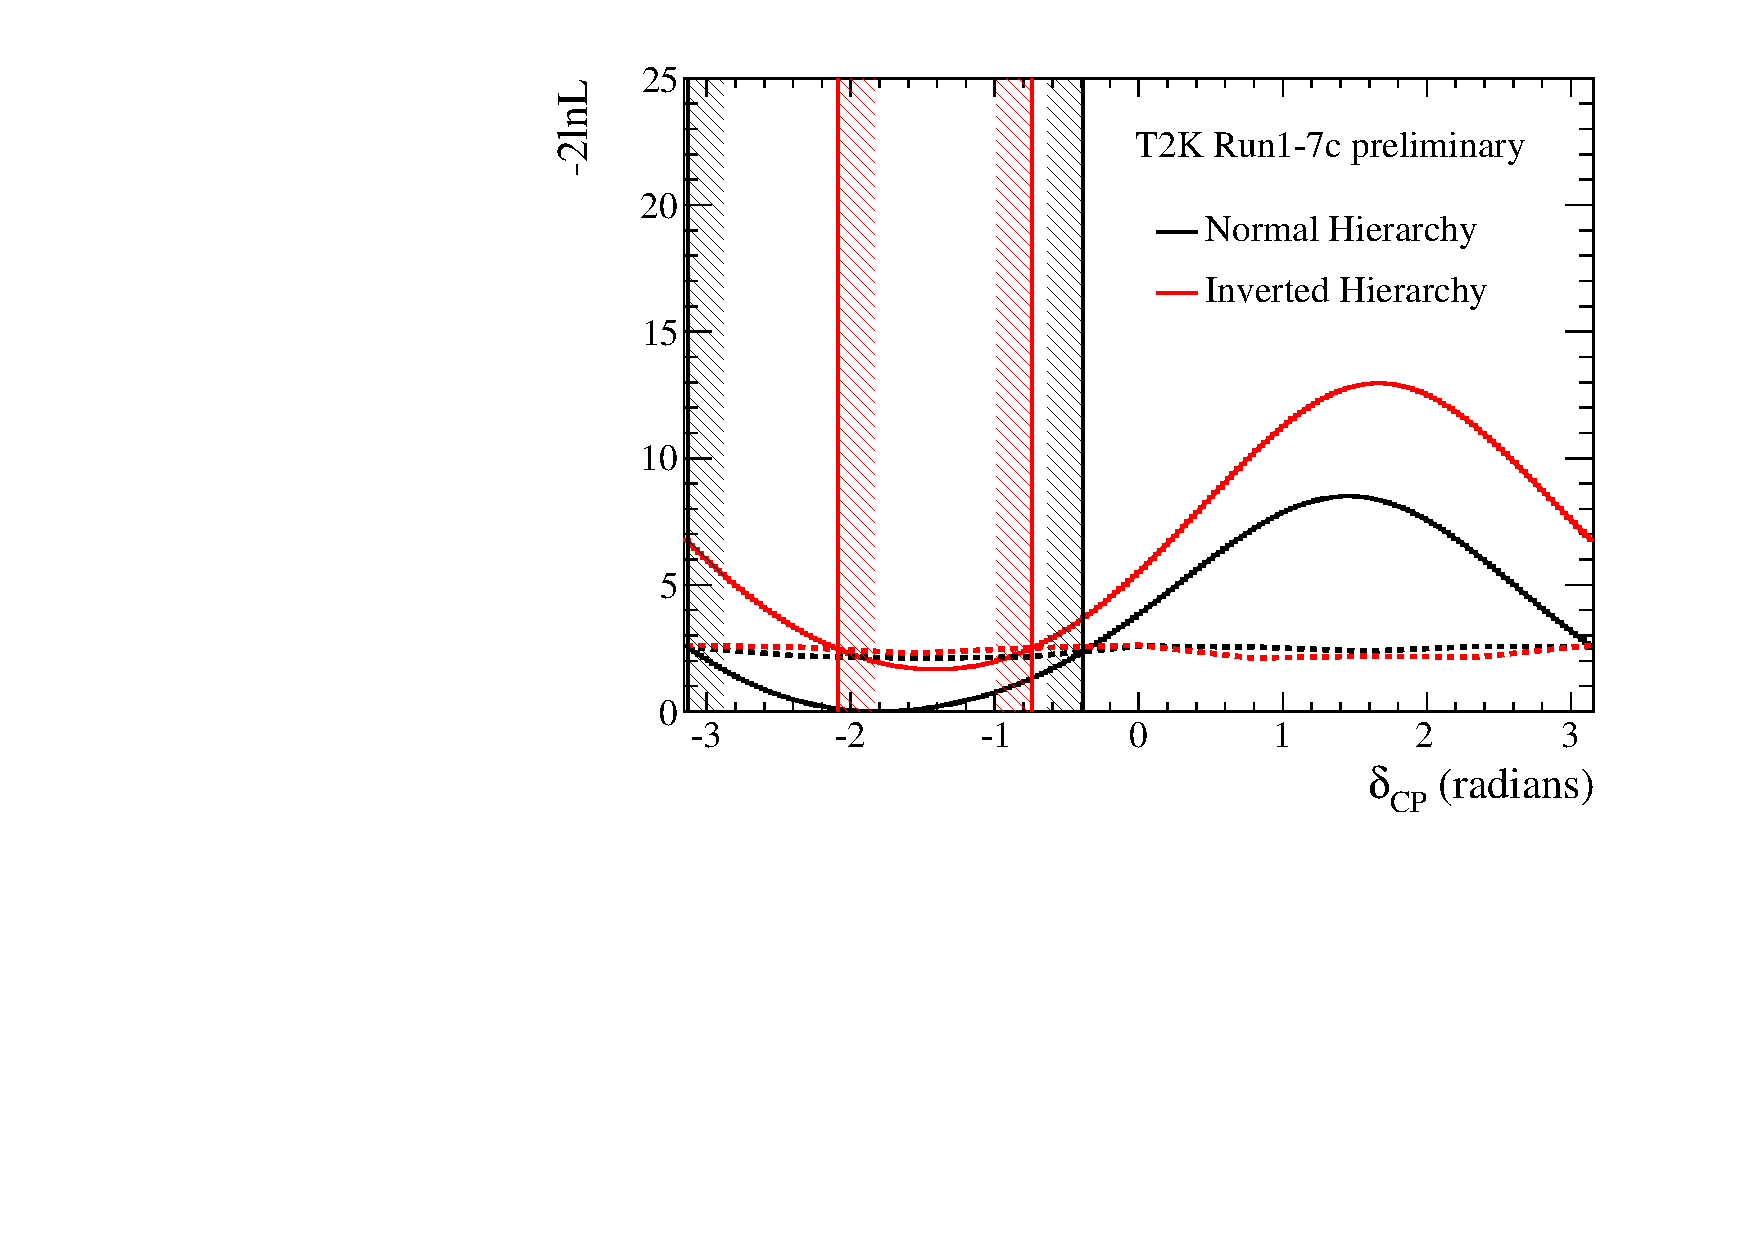
\includegraphics[width=0.49\textwidth]{joint_plots/coverage_fc/fc_run17c/dcp_mh_react_run17_interval_90CL.pdf} 
%\caption{
%Measured $\Delta \chi^2$ distributions with the full Run 1-7c data set.
%Both normal (black solid line) and inverted (black dashed line) hierarchies are shown. 
%The ``Feldman-Cousins" method is used to set the $\Delta \chi^2$ critical values in order to provide 
%confidence intervals with the proper coverage.
%The ranges of $\delta_{CP}$ which correspond to $\Delta \chi^2$ values larger than the critical 
%values (blue for 90\% CL and orange for $2\sigma$ CL) are excluded at a certain confidence level.
%Both normal and inverted hierarchy $\Delta \chi^2$ distributions are shifted with respect to the same global minimum. 
%All the oscillation parameters which are not parameters of interest
%are marginalised using the prior distributions shown in \cref{tab:marg_binnning}.
%The $\pm1 \sigma$ error on the critical values is shown as well, where specified, 
%and is represented by the lowest and highest set of critical values, with the same colour of the central ones.
%On the right plot a zoom on the critical values is shown.
%}
%\label{fig:joint_dcp_fc_run17c}
%\end{figure*}
%
%
%
%In \cref{tab:joint_bestfit_dcp_90CL_interval_FC_run17c} the 90\% CL intervals for $\delta_{CP}$ vs mass hierarchy,
%obtained with the Feldman-Cousins method, are shown.
%
%
%% Interval of deltaCP for 90% CL w/ Feldman-Cousins
%
%\begin{table}[htb]
%\centering
%\begin{tabular}{| c | c | c | c |}
%\hline
%{\bf Parameter}						& {\bf Reactors}		& {\bf Normal Hierarchy}		& {\bf Inverted Hierarchy}		\\
%\hline
%$\delta_{CP}$ (radians) 				& YES      			& [-3.13; -0.39]				& [-2.09; -0.74]				\\
%\hline
%\end{tabular}
%\caption{
%The confidence intervals at 90\% CL obtained with the Feldman-Cousins method
%for the Run 1-7c data set
%is shown for the measurement of $\delta_{CP}$ vs mass hierarchy.
%The reactor constraint $\sin^2 2\theta_{13} = 0.085 \pm 0.005 $ \cite{pdg_2014} is applied.
%}                                                                                                                                                                                          
%\label{tab:joint_bestfit_dcp_90CL_interval_FC_run17c}
%\end{table}
%
%
%\clearpage




















%--------------------------------------------------------------------------------------
%
% Contours
%
%--------------------------------------------------------------------------------------

\subsection {2-dimensional confidence intervals}
\label{sec:results_2d_contours_run17c}

The same 2-dimensional confidence intervals as in \cref{sec:results_2d_contours} are produced.
In \cref{fig:joint_sensi_t2krun14bf_2d_run17c} the corresponding 2-dimensional contours produced
with the Run 1-7c data set are shown drawing the normal and inverted hierarchy contours independently,
i.e. each contour is produced with respect to the global minimum under that hierarchy hypothesis.
In \cref{fig:joint_sensi_t2krun14bf_2d_glob} both normal and inverted hierarchy contours
are produced with respect to the same global minimum, i.e. the normal hierarchy hypothesis.
As already explained in \cref{sec:cl_mh}, ``global" and ``independent" contours correspond
respectively to the least and most conservative approach.

As in 1-dimensional analysis results
in \cref{fig:joint_data_fit_1d_run17c}, the reactor measurements are 
in agreement with the T2K data at $1\sigma$ level if $\delta_{CP} \sim - \frac{\pi}{2}$. 
Compared to \cref{fig:joint_sensi_t2krun14bf_2d}, both the normal and inverted 
hierarchy contours are closer to the reactor measurement.
Furthermore we can see that the region close $\delta_{CP} = + \pi/2$ is excluded at 90\% CL.

In \cref{fig:dcp_run17c_1ring_comparison,2d_reactors_run17c_1ring_comparison,fig:2d_t2konly_run17c_1ring_comparison}
we see the comparison of the results from the 1Ring only analysis with the 1Ring+\nueCConepi{} analysis. The improvement in the
constraints are comparable to the results from the sensitivity study comparison shown in \cref{sec:sensi_run17c}. The constraint 
on $\delta_{cp}$ is slightly stronger than expected which is due to the upward fluctuation observed in the \nueCConepi{} sample 
where 5 events were observed with only 3 expected. With this, there is a noticeably greater exclusion of $\delta_{CP}=\frac{\pi}{2}$.
The effect is also apparent in the $\sin^2 \theta_{13}$ Vs $\delta_{CP}$ contours where the new analysis prefers a larger value
of $\sin^2 \theta_{13}$ which, when constrained by the reactor measurements, results in a stronger constraint on $\delta_{CP}$. 
The comparison of the fits to $\sin^2 \theta_{23}$ Vs $\Delta m^2_{32}$ are slightly unexpected considering the sensitivity study, however the result where a greater portion of the lower octant of $\sin^2 \theta_{23}$ is excluded at 90\%CL and 68\%CL can be explained again by the excess of events observed in the \nueCConepi{}  which favour a much larger value of $\sin^2 \theta_{23}$ and therefore push the parameter to the upper octant. 

%As a result, we see that all $\delta_{CP}$ constraints in 
%\cref{fig:ss13_dcp_with_reactor_data_fit},~\ref{fig:dmsq_dcp_with_reactor_data_fit},~\ref{fig:ss23_dcp_with_reactor_data_fit} 
%are tighter for the inverted hierarchy hypothesis than for the normal.
%\cref{fig:dmsq_dcp_with_reactor_data_fit} also shows a slight anti-correlation between $\delta_{CP}$ 
%and $\Delta m^2_{32}$ in the normal hierarchy fit and a correlation in the inverted most likely coming 
%from the fact that $\Delta m^2_{32}$ and $cos(\delta_{CP})$ have similar effects on the shape of the appearance spectra. 
%In \cref{fig:ss23_dcp_with_reactor_data_fit} we see correlation where the constraint on $\delta_{CP}$ is narrower 
%for smaller values of $\sin^2 \theta_{23}$ as they both appear in the appearance term. 
%In \cref{fig:ss23_dmsq_with_reactor_data_fit} we see that $\sin^2 \theta_{23}$ and $\Delta m^2_{32}$ 
%are not very correlated however the inverted hierarchy contour is shifted down in $\Delta m^2_{32}$ 
%with respect to the normal hierarchy contour. 
%This effect is due to the correlation between $\Delta m^2_{32}$ and the mass hierarchy shown in \cref{fig:mass_hierarchy_MC_shift}. 
%Indeed the inverted hierarchy hypothesis produces an event migration toward higher energy 
%which is balanced in the fit by a lower fit value of $\Delta m^2_{13}$ with respect to the normal hierarchy case.

\begin{figure*}[htb]
\center
\begin{subfigure}[b]{0.49\textwidth}
%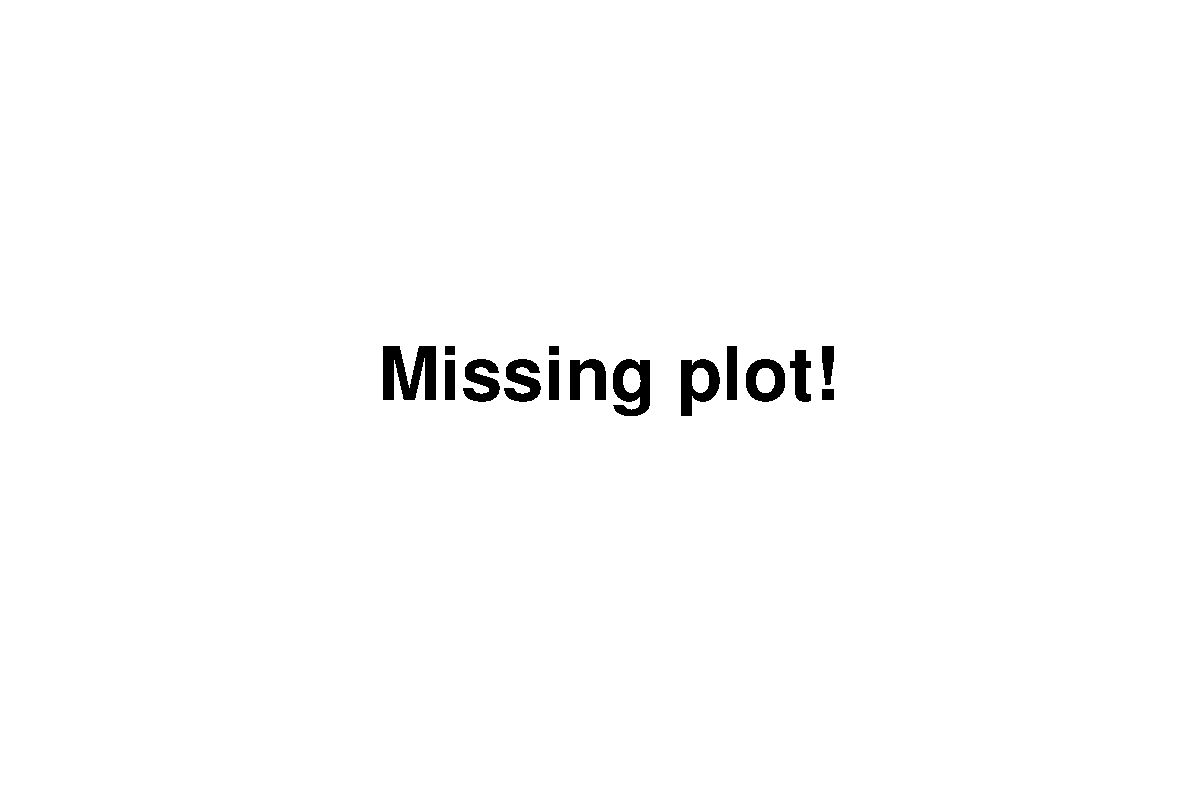
\includegraphics[width=0.9\textwidth]{./images/missing_plot-eps-converted-to.pdf}
\includegraphics[width=0.9\textwidth]{joint_plots/data_contours/Run17c/2D/cp_13.pdf}
\caption{$\sin^2 \theta_{13}$ vs $\delta_{CP}$ with T2K data only}
\label{fig:ss13_dcp_t2k_only_data_fit_run17c}
\end{subfigure}
\begin{subfigure}[b]{0.49\textwidth}
\includegraphics[width=0.9\textwidth]{joint_plots/data_contours/Run17c/2D/cp_13_reactor.pdf}
\caption{$\sin^2 \theta_{13}$ vs $\delta_{CP}$ with reactor constraint}
\label{fig:ss13_dcp_with_reactor_data_fit_run17c}
\end{subfigure}
\begin{subfigure}[b]{0.49\textwidth}
\includegraphics[width=0.9\textwidth]{joint_plots/data_contours/Run17c/2D/dmsq_dcp.pdf}
\caption{$\Delta m^2_{32}$ ($\Delta m^2_{13}$) vs $\delta_{CP}$ with reactor constraint}
\label{fig:dmsq_dcp_with_reactor_data_fit_run17c}
\end{subfigure}
\begin{subfigure}[b]{0.49\textwidth}
\includegraphics[width=0.9\textwidth]{joint_plots/data_contours/Run17c/2D/ss23_dcp.pdf}
\caption{$\sin^2 \theta_{23}$ vs $\delta_{CP}$ with reactor constraint}
\label{fig:ss23_dcp_with_reactor_data_fit_run17c}
\end{subfigure}
\begin{subfigure}[b]{0.49\textwidth}
\includegraphics[width=0.9\textwidth]{joint_plots/data_contours/Run17c/2D/ss23_dmsq.pdf}
\caption{$\sin^2 \theta_{23}$ vs $\Delta m^2_{32}$ ($\Delta m^2_{13}$)
with reactor constraint}
\label{fig:ss23_dmsq_with_reactor_data_fit_run17c}
\end{subfigure}
\caption{
%{\large{MEASURED 2D CONTOURS}}
Measured confidence intervals with the full Run 1-7c data set.
Both normal (black) and inverted (red) hierarchies are shown. 
Both 68\% (dashed line) and 90\% CL (solid line) are shown.
Confidence intervals are produced using the \emph{constant} $\Delta \chi^2$ method. % (see \cref{app:method_cl}).
Contours for normal (black) and inverted (red) hierarchy are computed independently.
All the oscillation parameters which are not parameters of interest
are marginalised using the prior distributions shown in \cref{tab:osc_params_joint_priors}.
The measured contour of $\sin^2 \theta_{13}$ vs $\delta_{CP}$ without reactor constraint, in \cref{fig:ss13_dcp_t2k_only_data_fit} is compared with the measurement by reactor experiments, 
$\sin^2 \theta_{13} = 0.0219 \pm 0.0012 $
\cite{pdg_2014},
shown by the yellow bar.
}
\label{fig:joint_sensi_t2krun14bf_2d_run17c}
\end{figure*}


\begin{figure*}[htb]
\center
\begin{subfigure}[b]{0.49\textwidth}
%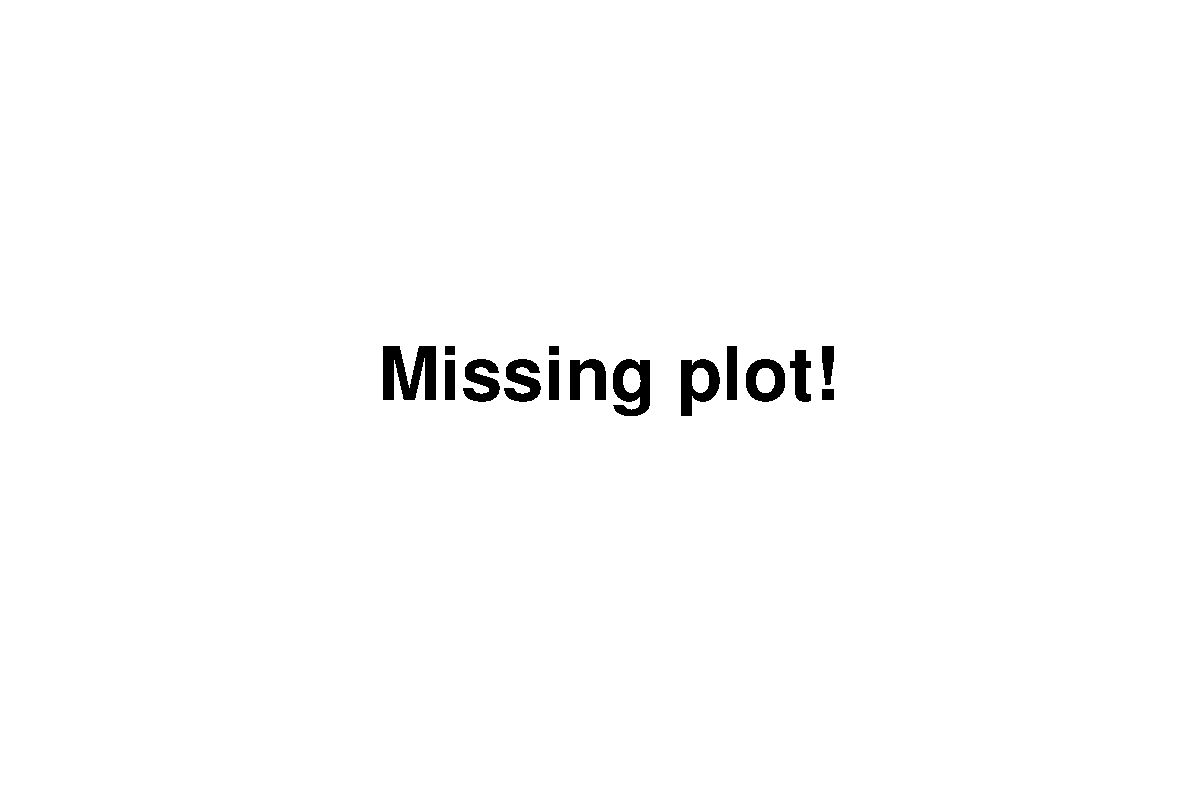
\includegraphics[width=0.9\textwidth]{./images/missing_plot-eps-converted-to.pdf}
\includegraphics[width=0.9\textwidth]{joint_plots/data_contours/Run17c/2D/cp_13_glob.pdf}
\caption{$\sin^2 \theta_{13}$ vs $\delta_{CP}$ with T2K data only}
\label{fig:ss13_dcp_t2k_only_data_fit_run17c}
\end{subfigure}
\begin{subfigure}[b]{0.49\textwidth}
\includegraphics[width=0.9\textwidth]{joint_plots/data_contours/Run17c/2D/cp_13_reactor_glob.pdf}
\caption{$\sin^2 \theta_{13}$ vs $\delta_{CP}$ with reactor constraint}
\label{fig:ss13_dcp_with_reactor_data_fit_run17c}
\end{subfigure}
\begin{subfigure}[b]{0.49\textwidth}
\includegraphics[width=0.9\textwidth]{joint_plots/data_contours/Run17c/2D/dmsq_dcp_glob.pdf}
\caption{$\Delta m^2_{32}$ ($\Delta m^2_{13}$) vs $\delta_{CP}$ with reactor constraint}
\label{fig:dmsq_dcp_with_reactor_data_fit_run17c}
\end{subfigure}
\begin{subfigure}[b]{0.49\textwidth}
\includegraphics[width=0.9\textwidth]{joint_plots/data_contours/Run17c/2D/ss23_dcp_glob.pdf}
\caption{$\sin^2 \theta_{23}$ vs $\delta_{CP}$ with reactor constraint}
\label{fig:ss23_dcp_with_reactor_data_fit_run17c}
\end{subfigure}
\begin{subfigure}[b]{0.49\textwidth}
\includegraphics[width=0.9\textwidth]{joint_plots/data_contours/Run17c/2D/ss23_dmsq_glob.pdf}
\caption{$\sin^2 \theta_{23}$ vs $\Delta m^2_{32}$ ($\Delta m^2_{13}$)
with reactor constraint}
\label{fig:ss23_dmsq_with_reactor_data_fit_run17c}
\end{subfigure}
\caption{
%{\large{MEASURED 2D CONTOURS}}
Measured confidence intervals with the full Run 1-7c data set.
Both normal (black) and inverted (red) hierarchies are shown. 
Both 68\% (dashed line) and 90\% CL (solid line) are shown.
Confidence intervals are produced using the \emph{constant} $\Delta \chi^2$ method. % (see \cref{app:method_cl}).
Contours for normal (black) and inverted (red) hierarchy are computed with respect to the minimum $\chi^2$ 
in both hierarchies.
All the oscillation parameters which are not parameters of interest
are marginalised using the prior distributions shown in \cref{tab:osc_params_joint_priors}.
The measured contour of $\sin^2 \theta_{13}$ vs $\delta_{CP}$ without reactor constraint, in \cref{fig:ss13_dcp_t2k_only_data_fit} is compared with the measurement by reactor experiments, 
$\sin^2 \theta_{13} = 0.0219 \pm 0.0012 $
\cite{pdg_2014},
shown by the yellow bar.
}
\label{fig:joint_sensi_t2krun14bf_2d_run17c_glob}
\end{figure*}


\begin{figure*}[htb]
\center
\begin{subfigure}[b]{0.49\textwidth}
\includegraphics[width=0.9\textwidth]{./joint_plots/data_contours/Run17c/1D_comp/dcp_reactor_nh_a.pdf}
\caption{Normal hierarchy with the reactor constraint}
\end{subfigure}
\begin{subfigure}[b]{0.49\textwidth}
\includegraphics[width=0.9\textwidth]{./joint_plots/data_contours/Run17c/1D_comp/dcp_reactor_ih_a.pdf}
\caption{Inverted hierarchy with the reactor constraint}
\end{subfigure}
\begin{subfigure}[b]{0.49\textwidth}
\includegraphics[width=0.9\textwidth]{./joint_plots/data_contours/Run17c/1D_comp/dcp_nh_a.pdf}
%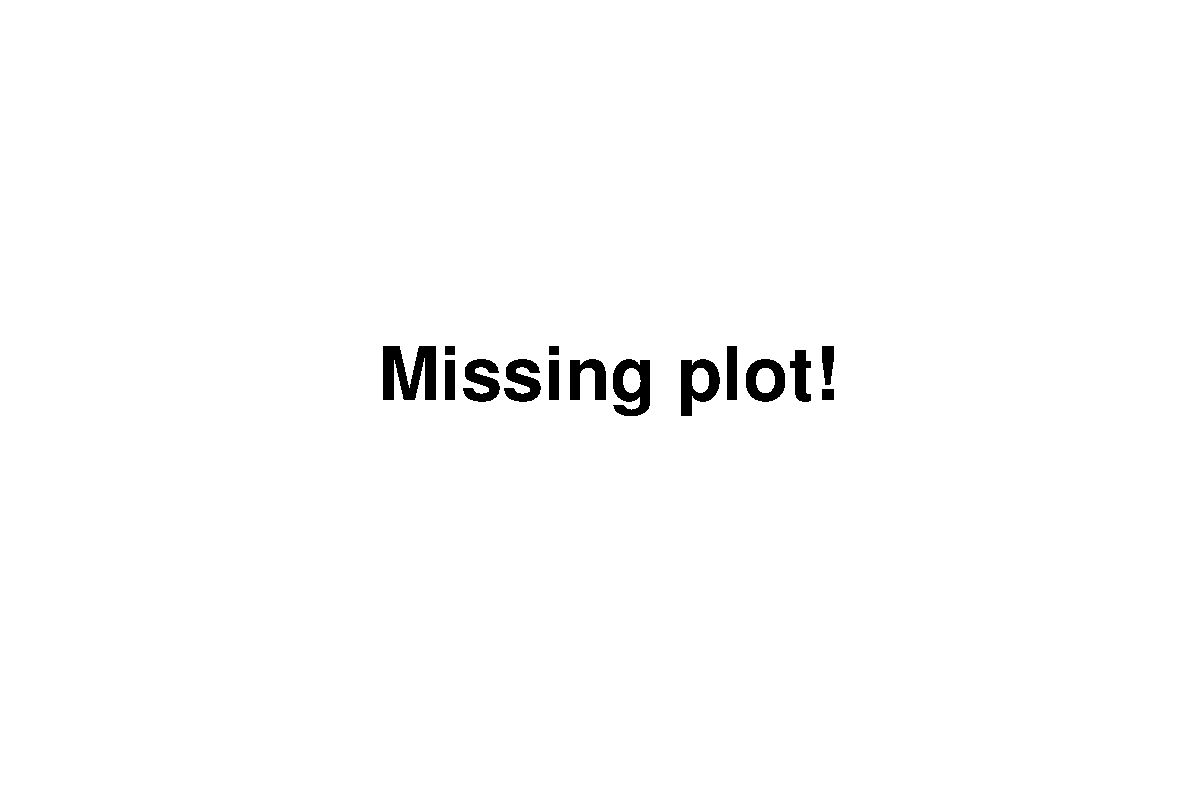
\includegraphics[width=0.9\textwidth]{./images/missing_plot-eps-converted-to.pdf}
\caption{Normal hierarchy without the reactor constraint}
\end{subfigure}
\begin{subfigure}[b]{0.49\textwidth}
\includegraphics[width=0.9\textwidth]{./joint_plots/data_contours/Run17c/1D_comp/dcp_ih_a.pdf}
%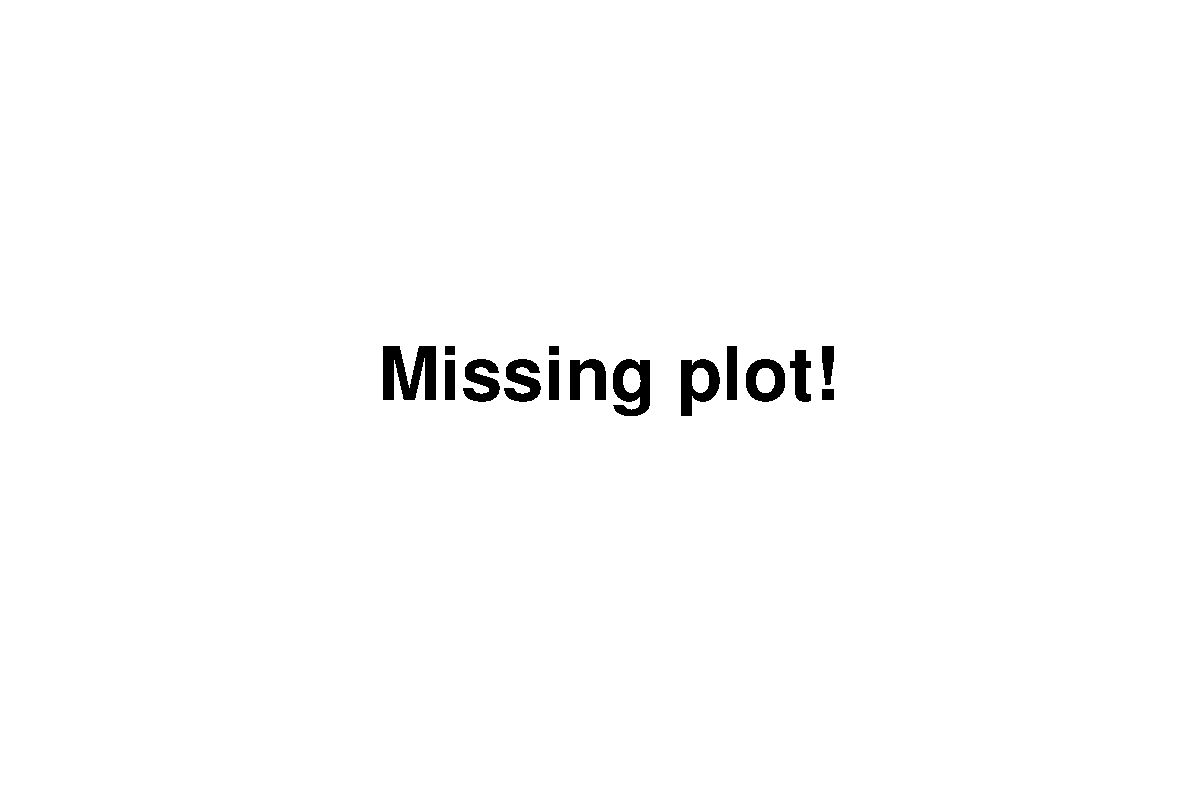
\includegraphics[width=0.9\textwidth]{./images/missing_plot-eps-converted-to.pdf}
\caption{Inverted hierarchy without the reactor constraint}
\end{subfigure}
\caption {
The comparison of the results of fits to $\delta_{cp}$
from the 1Ring and 1Ring+cc$\pi^+$ analyses are shown.
The comparison is done both applying the reactor constraint (top)
and with only T2K data (bottom)
}
\label{fig:dcp_run17c_1ring_comparison}
\end{figure*}

\begin{figure*}[htb]
\center
%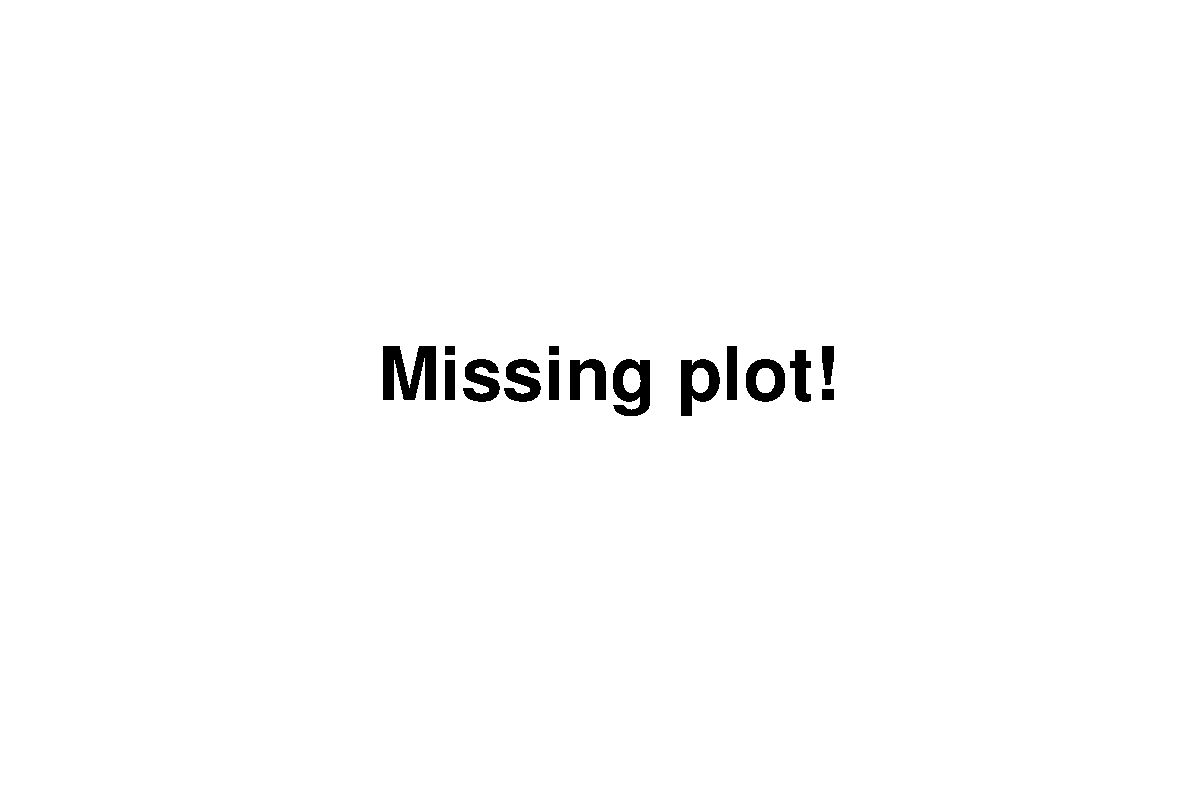
\includegraphics[width=0.9\textwidth]{./images/missing_plot-eps-converted-to.pdf}
%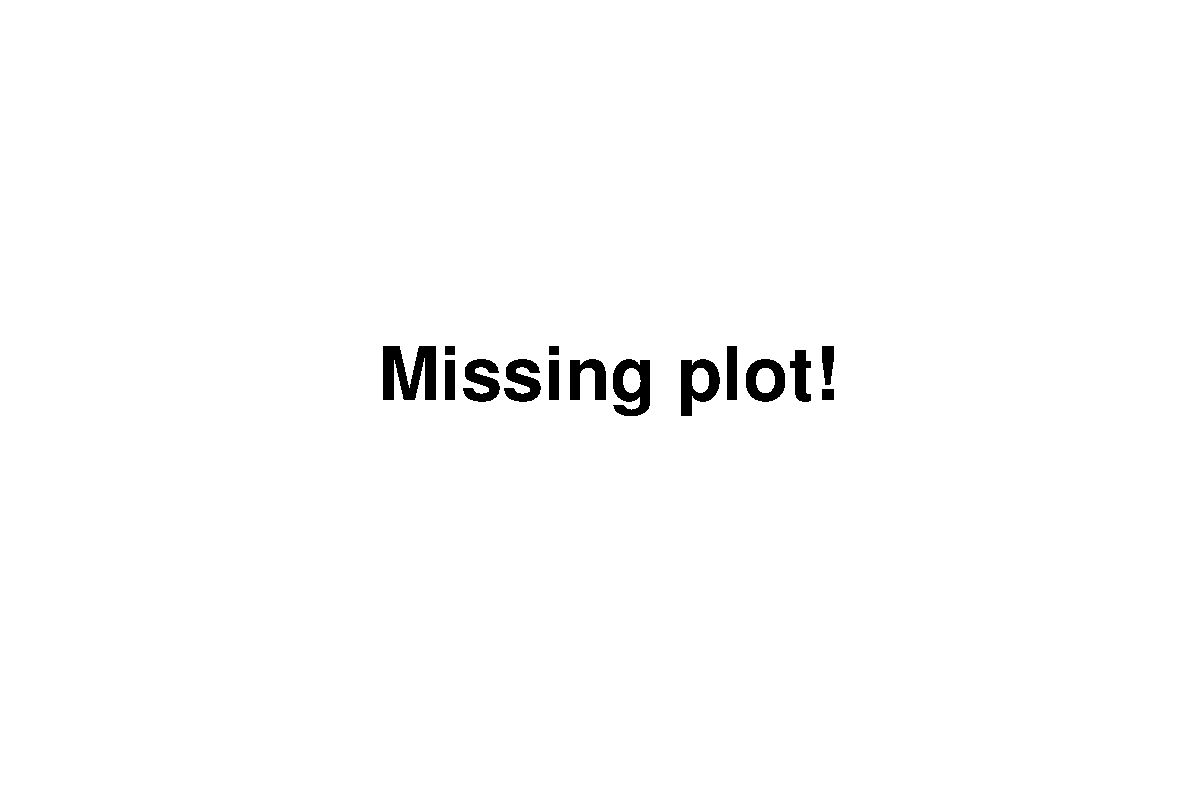
\includegraphics[width=0.9\textwidth]{./images/missing_plot-eps-converted-to.pdf}
%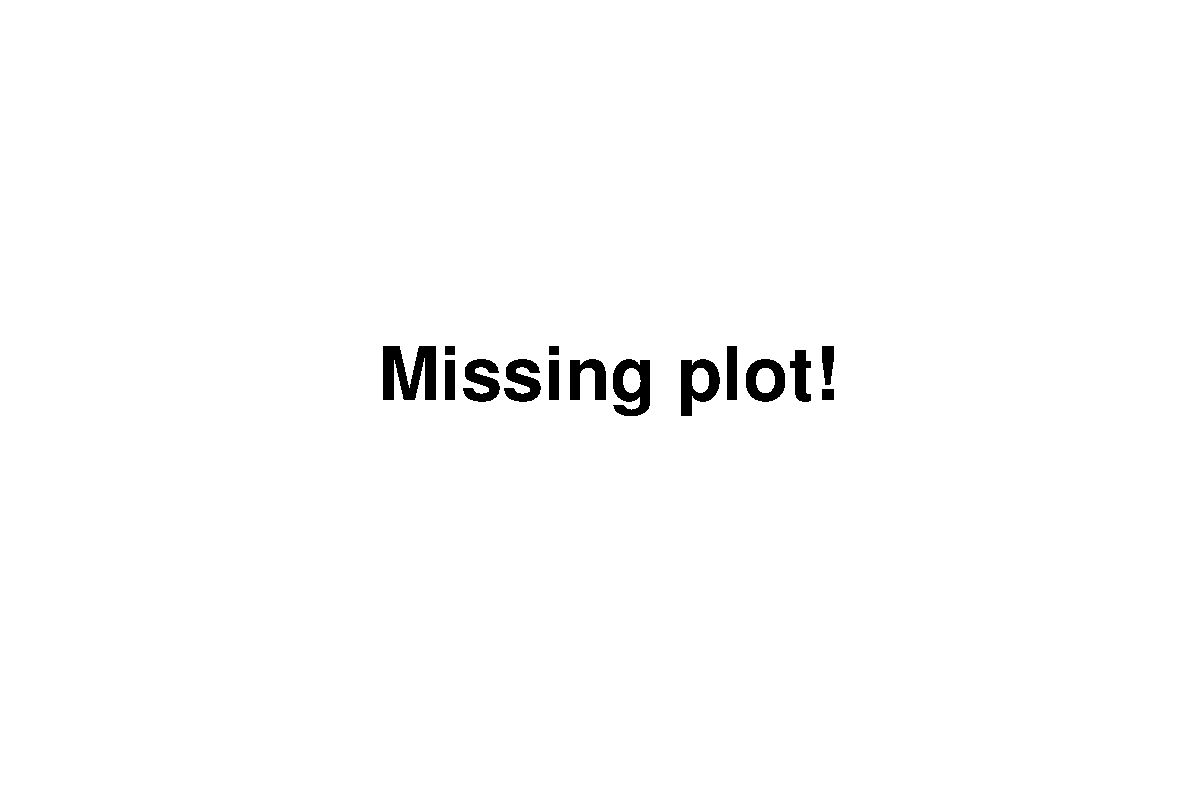
\includegraphics[width=0.9\textwidth]{./images/missing_plot-eps-converted-to.pdf}
\begin{subfigure}[b]{0.49\textwidth}
\includegraphics[width=0.9\textwidth]{./joint_plots/data_contours/Run17c/2D_comp/cp_13_reactor_nh_a.pdf}
\caption{Normal: $\sin^2 \theta_{13}$ Vs $\delta_{CP}$. }
\end{subfigure}
\begin{subfigure}[b]{0.49\textwidth}
\includegraphics[width=0.9\textwidth]{./joint_plots/data_contours/Run17c/2D_comp/cp_13_reactor_ih_a.pdf} 
\caption{Inverted: $\sin^2 \theta_{13}$ Vs $\delta_{CP}$. }
\end{subfigure}
\begin{subfigure}[b]{0.49\textwidth}
\includegraphics[width=0.9\textwidth]{./joint_plots/data_contours/Run17c/2D_comp/ss23_dmsq_nh_a.pdf}
\caption{Normal: $\sin^2 \theta_{23}$ Vs $\Delta m^2_{32}$ ($m^2_{13}$). }
\end{subfigure}
\begin{subfigure}[b]{0.49\textwidth}
\includegraphics[width=0.9\textwidth]{./joint_plots/data_contours/Run17c/2D_comp/ss23_dmsq_ih_a.pdf}
\caption{Inverted: $\sin^2 \theta_{23}$ Vs $\Delta m^2_{32}$ ($m^2_{13}$). }
\end{subfigure}
\caption {
%{\large{SENSI 2D CONTOURS W/ AND W/O REACTORS}}
The comparison of the results of fits 
from the 1Ring and 1Ring+cc$\pi^+$ analyses are shown.
The contours at 68\% and 90\% CL with reactor constraint 
the Run 1-7c statistics are shown.
%is compared to the result obtained by the other analysis groups.
}
\label{fig:2d_reactors_run17c_1ring_comparison}
\end{figure*}

\begin{figure*}[htb]
\center
\begin{subfigure}[b]{0.49\textwidth}
%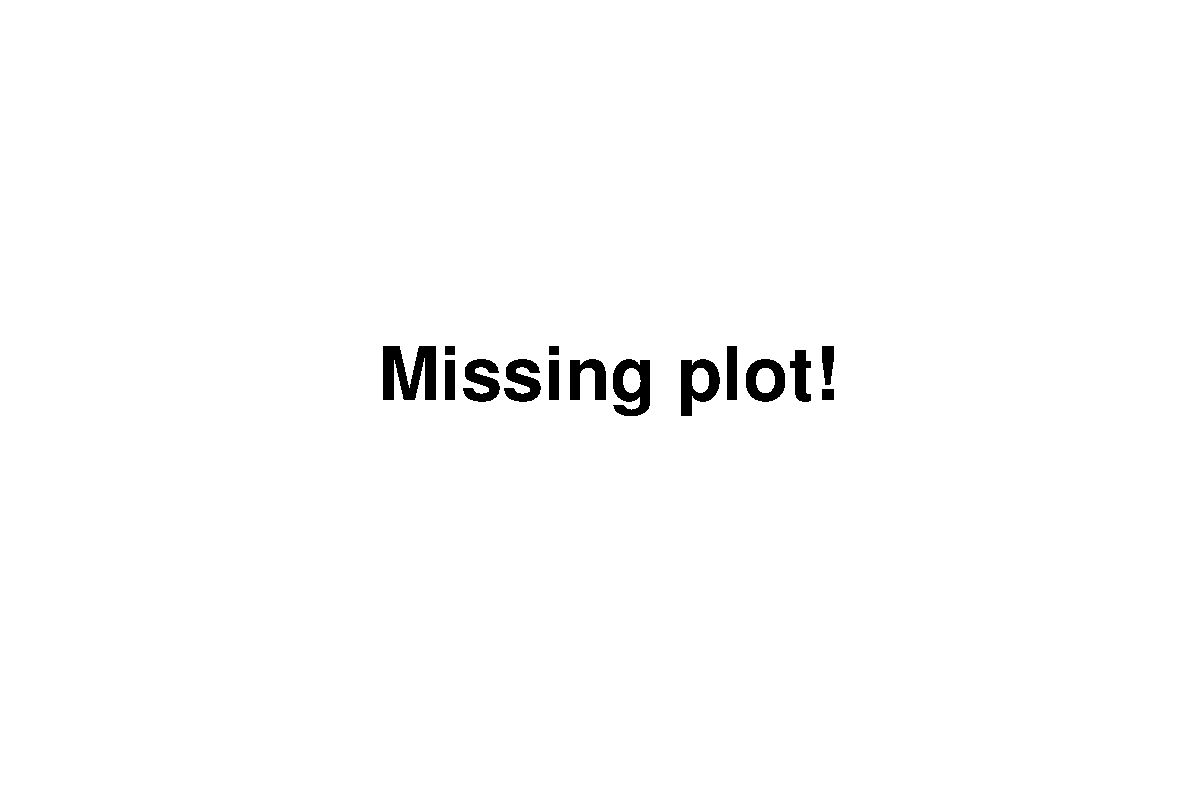
\includegraphics[width=0.9\textwidth]{./images/missing_plot-eps-converted-to.pdf}
\includegraphics[width=0.9\textwidth]{./joint_plots/data_contours/Run17c/2D_comp/cp_13_nh_a.pdf}
\caption{Normal}
\end{subfigure}
\begin{subfigure}[b]{0.49\textwidth}
%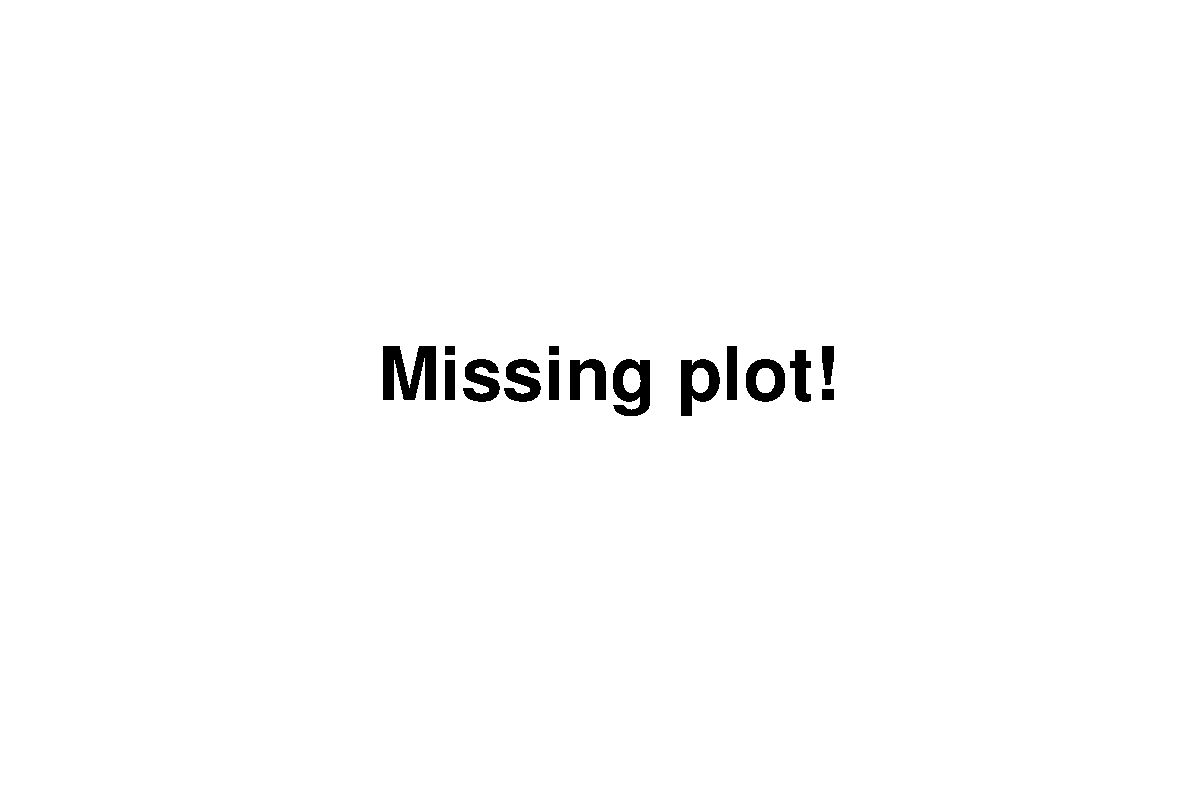
\includegraphics[width=0.9\textwidth]{./images/missing_plot-eps-converted-to.pdf}
\includegraphics[width=0.9\textwidth]{./joint_plots/data_contours/Run17c/2D_comp/cp_13_ih_a.pdf}
\caption{Inverted}
\end{subfigure}
\caption {
%{\large{SENSI 2D CONTOURS W/ AND W/O REACTORS}}
The comparison of the results of fits 
from the 1Ring and 1Ring+cc$\pi^+$ analyses are shown.
The contours at 68\% and 90\% CL for $\sin^2 \theta_{13}$ Vs $\delta_{CP}$
corresponding to the Run 1-7c statistics 
are shown.
%is compared to the result obtained by the other analysis groups.
Only T2K data are used.
}
\label{fig:2d_t2konly_run17c_1ring_comparison}
\end{figure*}


{\huge{TODO UPDATE other experiment comparison!!}}
%In \cref{fig:joint_sensi_ss23Vsdmsq_2d_run17c_othexp} the contours for  $\sin^2 \theta_{23}$ vs $\Delta m^2_{32}$ ($\Delta m^2_{13}$) with the full Run 1-7c data set
%are compared with the other experimental results.
%
%\begin{figure*}[htb]
%\center
%\begin{subfigure}[b]{0.59\textwidth}
%\includegraphics[width=0.9\textwidth]{joint_plots/data_contours/Run17c/sinsqth23Vsdmsq_react_OthExp_nh.pdf} 
%\includegraphics[width=0.9\textwidth]{joint_plots/data_contours/Run17c/sinsqth23Vsdmsq_react_OthExp_ih.pdf}
%\end{subfigure}
%\caption{
%The measured T2K confidence intervals for $\sin^2 \theta_{23}$ vs $\Delta m^2_{32}$ ($\Delta m^2_{13}$) with the full Run 1-7c data set are compared to the other experimental results.
%Both normal (top) and inverted (bottom) hierarchies are shown. 
%Both 68\% (dashed line) and 90\% CL (solid line) are shown.
%Confidence intervals are produced using the \emph{constant} $\Delta \chi^2$ method. % (see \cref{app:method_cl}).
%Contours for normal (black) and inverted (red) hierarchy are computed independently.
%All the oscillation parameters which are not parameters of interest
%are marginalised using the prior distributions shown in \cref{tab:osc_params_joint_priors}.
%The measured contour of $\sin^2 \theta_{13}$ vs $\delta_{CP}$ without reactor constraint, in \cref{fig:ss13_dcp_t2k_only_data_fit} is compared with the measurement by reactor experiments, 
%$\sin^2 \theta_{13} = 0.0219 \pm 0.0012 $
%\cite{pdg_2014},
%shown by the yellow bar.
%For normal hierarchy the other experiment results are: 
%Super-K (PoS ICRC2015 (2015) 1062), 
%Minos+ (Neutrino 2014 conference), 
%NO$\nu$A (Neutrino 2016 conference) and 
%IceCube DeepCore (Phys.Rev. D91 (2015) 072004, arXiv 1410.7227).
%For inverted hierarchy the other experiment results are: 
%Super-K (PoS ICRC2015 (2015) 1062) and Minos+ (Neutrino 2014 conference).
%}
%\label{fig:joint_sensi_ss23Vsdmsq_2d_run17c_othexp}
%\end{figure*}

\clearpage














%...........................................................
%
% Discussion about the results
%
%...........................................................

\subsection {Discussion of the Run 1-7c data fit results}
\label{sec:results_discussion_run17c}

Using the additional cc$\pi^+$ data set we see an excess in the number of observed appearance 
events which is consistent with what is seen in the neutrino mode one ring $e$-like sample. 

The value of $\delta_{CP}$ favoured by the joint fit analysis, when the reactor constraint is applied, 
is -1.728 and corresponds to normal hierarchy.
$\delta_{CP} = 0$ is excluded at more than 2 standard deviations and a large fraction of the range between $\delta_{CP} = 0$ and $+\pi$
is excluded with a significance of $2 \sigma$, as for the previous analyses.

The inverted hierarchy is disfavoured at about 90\%CL and is partially 
excluded at $3\sigma$ for values of $\delta_{CP}$ around $+\pi/2$ similarly as for 1 ring data set.
%This exclusion, stronger than what is expected from the fit of the Asimov data sets for $\delta_{CP}=-1.601$,
%is due to an excess of events in neutrino mode and, additionally to Run 1-6, 
%to a small deficit of events in the antineutrino mode $e$-like sample.

If the reactor constraint is not applied, the best-fit value of $\delta_{CP}$ is still quite close to $-\pi/2$
and $\delta_{CP}=0$ is still excluded at about 90\% CL (using constant $\Delta \chi^2$ method).

The contour of $\sin^2 \theta_{13}$ vs $\delta_{CP}$ shows a very good agreement (within $1 \sigma$),
with the measurement of the reactor experiments.


\clearpage






% Run 1-7b update
\clearpage

% --------------------------------------------------------------------------------------------

\section{Summary}
\label{sec:summary}

In this technical note,
we have presented the results of the 3-flavour $\bar{\nu}/\nu$ joint analysis
performed by the {\em VALOR} group,
on the combined Run 1-7c data set.
%for an exposure of \TotalPotNu{} POT in neutrino mode
%and \TotalPotNuBar{} POT in antineutrino mode. 
The goal of the analysis is to search for CP violation in the leptonic
and put limits on $\delta_{CP}$ as well as 
measure all the other oscillation parameters to which T2K is sensitive:
$\sin^2 \theta_{13}$, $\sin^2 \theta_{23}$, $\Delta m^2_{32}$ ($\Delta m^2_{13}$)
and partially mass hierarchy, to which T2K has little sensitivity.

This analysis predicts 
\NskOscExpectationNumuRunOneSevenC{} $\pm$ \NskOscExpectationNumuErrorRunOneSevenC{} (syst) for neutrino $\mu$-like,
\NskOscExpectationNumuBarRunOneSevenC{} $\pm$ \NskOscExpectationNumuBarErrorRunOneSevenC{} (syst) for antineutrino $\mu$-like,
\NskOscExpectationNueRunOneSevenC{} $\pm$ \NskOscExpectationNueErrorRunOneSevenC{} (syst) for neutrino $e$-like,
\NskOscExpectationNueBarRunOneSevenC{} $\pm$ \NskOscExpectationNueBarErrorRunOneSevenC{} (syst) for antineutrino $e$-like
and 
\NskOscExpectationNueCConepiRunOneSevenC{} $\pm$ \NskOscExpectationNueCConepiErrorRunOneSevenC{} (syst) for   neutrino \nueCConepi{}
events in Super K
and observes respectively 
\NskObservedNumuRunOneSevenC{} for neutrino $\mu$-like,
\NskObservedNumuBarRunOneSevenC{}  for antineutrino $\mu$-like,
\NskObservedNueRunOneSevenC{}  for neutrino $e$-like,
\NskObservedNueBarRunOneSevenC{}  for antineutrino $e$-like
and 
\NskObservedNueCConepiRunOneSevenC for neutrino \nueCConepi{}. 

The $\bar{\nu}/\nu$ analysis was performed
in a framework of 3-flavour oscillations including matter effects in constant-density matter.
The observed reconstructed energy spectrum of single $\mu$-like ring events
and reconstructed energy versus lepton angle of single $e$-like ring events
was used to compute the confidence intervals.
All \NSyst{} systematic parameters as well as the oscillation parameters
which were not parameters of interest considered in this analysis were marginalised.

From the fit of the Run 1-67c data we can see that the favoured value of $\delta_{CP}$ is xxx, close to $-\pi/2$.
The correct coverage is provided by using the ``Feldman-Cousins" method with which the 
significance to excluded $\delta_{CP}=0$ becomes XXX standard deviations,
while $\delta_{CP}=\pi$ is excluded at less than 90\% CL.
The Run 1-6 data do not exclude the hypothesis of CP conservation. 

%When the constant $\Delta \chi^2$ method is used $\delta_{CP}=0$ is excluded at 90\% CL
%and a large portion between $0$ and $+\pi$ is excluded at $2\sigma$ if normal hierarchy is considered.
In case of inverted hierarchy a not negligible range of $\delta_{CP}$ around $+\pi/2$ is excluded with 
a significance of $3\sigma$.

From the contour of $\sin^2 \theta_{13}$ vs $\delta_{CP}$ without the reactor constraint 
it is clear that the T2K data are in agreement with the reactor measurements within $1\sigma$ 
if $\delta_{CP} \sim -\pi/2$.

It has also been shown that the result of the search for CP violation is dominated by the excess of event in the neutrino mode
$e$-like sample, though the antineutrino mode $e$-like also prefers values of $\delta_{CP}$ close to $-\pi/2$.
However the significance is not high.



\clearpage


% References
%
% References
%

\begin{thebibliography}{9}

%
% Our previous analyses
%
\bibitem{OurRun1DisappAnalysis}
   C.Andreopoulos, T.Dealtry, J.Dobson, N.Grant, M.Haigh, J.Ilic, G.Pearce and A.Weber,
   T2K 3.23$\times10^{19}$-POT Muon-Neutrino Disappearance Analysis,
   T2K-TN-036(v4),\\
   http://www.t2k.org/docs/technotes/036
\bibitem{OurRun12DisappAnalysis}
   C.Andreopoulos, T.Dealtry, J.Dobson, N.Grant, M.Haigh, J.Ilic, G.Pearce and A.Weber,
   T2K 1.431$\times10^{20}$-POT Muon-Neutrino Disappearance Analysis
   T2K-TN-064(v3),\\
   http://www.t2k.org/docs/technotes/064
\bibitem{OurRun12DisappAnalysis3Flavour}
   C.Andreopoulos, T.Dealtry, L.Escudero, N.Grant and A.Weber,
   T2K 1.431$\times10^{20}$-POT 3-Flavour Muon-Neutrino Disappearance Analysis
   T2K-TN-087(v1),\\
   http://www.t2k.org/docs/technotes/087
\bibitem{OurRun123DisappAnalysis3Flavour}
   C.Andreopoulos, T.Dealtry, L.Escudero, N.Grant and A.Weber,
   T2K 3.010$\times10^{20}$-POT 3-Flavour Muon-Neutrino Disappearance Analysis
   T2K-TN-141(v10),\\
   http://www.t2k.org/docs/technotes/141
\bibitem{OurRun1234aDisappAnalysis3Flavour}
   C.Andreopoulos, T.Dealtry, L.Escudero, N.Grant and A.Weber,
   T2K 6.3933$\times10^{20}$-POT 3-Flavour Muon-Neutrino Disappearance Analysis
   T2K-TN-155(v2),\\
   http://www.t2k.org/docs/technotes/155
\bibitem{OurRun1234DisappAnalysis3Flavour}
   C.Andreopoulos, T.Dealtry, L.Escudero, N.Grant and A.Weber,
   T2K 6.57$\times10^{20}$-POT 3-Flavour Muon-Neutrino Disappearance Analysis
   T2K-TN-183(v3),\\
   http://www.t2k.org/docs/technotes/183
\bibitem{OurRun123JointOscillationAnalysis}
   C.Andreopoulos et al.,
   T2K 3.010$\times10^{20}$-POT Joint 3-Flavour Oscillation Analysis
   T2K-TN-154(v3),\\
   http://www.t2k.org/docs/technotes/154
\bibitem{OurRun1234JointOscillationAnalysis}
   C.Andreopoulos et al.,
   T2K 6.57$\times10^{20}$-POT Joint 3-Flavour Oscillation Analysis
   T2K-TN-175,\\
   http://www.t2k.org/docs/technotes/175
\bibitem{OurRun56AntiNumuDisappearanceAnalysis3Flavour}
   C.Andreopoulos et al.,
   T2K 2.315$\times10^{20}$-POT 3-Flavour Muon-Antineutrino Disappearance Analysis
   T2K-TN-243,\\
   http://www.t2k.org/docs/technotes/243
\bibitem{OurRun56AntiNueBarAppearanceAnalysis3Flavour}
   C.Andreopoulos et al.,
   T2K 4.0108$\times10^{20}$-POT 3-Flavour Electron-Antineutrino Appearance Analysis
   T2K-TN-252,\\
   http://www.t2k.org/docs/technotes/252
\bibitem{OurRun1617b17cJointAnalysis3Flavour}
   C.Andreopoulos et al.,
   T2K Neutrino and Anti-Neutrino 3-Flavour Joint Analysis of  \\
   Run 1-6  (6.914$\times10^{20}$-POT $\nu$ 4.011$\times10^{20}$-POT $\bar{\nu}$), \\
   Run 1-7b (7.002$\times10^{20}$-POT $\nu$ 7.471$\times10^{20}$-POT $\bar{\nu}$) and \\
   Run 1-7c (7.482$\times10^{20}$-POT $\nu$ 7.471$\times10^{20}$-POT $\bar{\nu}$)
   data sets
   T2K-TN-266,\\
   http://www.t2k.org/docs/technotes/266
%
% Supplementary material to this analysis
%
\bibitem{OurRun1234DisappAnalysisSupplement}
  C.Andreopoulos, T.Dealtry, L.Escudero and N.Grant,
  T2K 6.5700$\times10^{20}$-POT 3-Flavour Muon-Neutrino Disappearance Analysis:
  Supplementary material on the effect of systematics,
  T2K-TN-183 supplement,\\
  http://www.t2k.org/docs/technotes/183

%
% Our previous published analyses
%
\bibitem{T2KRun12Disapp}
   T2K Collaboration (K.Abe et al.), 
   First Muon-Neutrino Disappearance Study with an Off-Axis Beam,
   Phys.Rev.D85:031103, 2012; arXiv:1201.1386
\bibitem{T2KRun123Disapp}
  T2K Collaboration (K.Abe et al.),
  Measurement of Neutrino Oscillation Parameters from Muon Neutrino Disappearance with an Off-axis Beam,
  arXiv:1308.0465 [hep-ex], 2013.
  
%
% T2K papers and drafts
%
t2k neutrino\bibitem{T2KLongPaper}
   T2K Collaboration (K.Abe et al.),
   Measurement of neutrino oscillation in appearance and disappearance channels by the T2K experiment with 
   6.6$\times$10$^{20}$ protons on target 
   http://www.t2k.org/comm/pubboard/JournalPapers/oa2014prd/draft3

%
% p-theta TN
%
\bibitem{ptheta}
J. Imber et al.,
Four Sample Joint Oscillation Analysis with T2K Run1-6 Data,
  T2K-TN-267,\\
 http://www.t2k.org/docs/technotes/267

%
% Official 2012 analysis inputs and software packages
%
\bibitem{Neut:ActaP}
  Y.Hayato, A neutrino interaction simulation program library NEUT,
  Acta Phys.Polon.B40:2477-2489,2009.
\bibitem{FluxTuning}
   Beam WG, Flux tuning (11b v3.2), http://www.t2k.org/beam/NuFlux/FluxRelease/11brelease/11btuned-v3.2
\bibitem{SuperkErrors}
   M.Otani and J.Kameda,
   Super-K events and Updated systematic errors for $\nu_\mu$ disappearance analysis with T2K 1.431$\times10^{20}$ POT
   T2K-TN-065(v6),
   http://www.t2k.org/docs/technotes/065
\bibitem{NEUTnuclear}
  P. de Perio et al.,
  NEUT nuclear effects (FSI)
  T2K-TN-033(v2.0),
  http://www.t2k.org/docs/technotes/033
\bibitem{NIWGErr}
  P. de Perio et al.,
  Cross section parameters for the 2012a oscillation analysis
  T2K-TN-108(v1.3),
  http://www.t2k.org/docs/technotes/108
\bibitem{MoreNIWGErr113}
  P. de Perio et al.,
  Implementation of the NIWG cross-section parametrization,
  T2K-TN-113(v1.2) 
\bibitem{NIWGNuBarErr}
  Y.Hayato, K.McFarland, and M.Wascko (Private communication) 
% \bibitem{BANFF}
%   P. de Perio et al.,
%   Constraining the Flux and Cross Section Models with Data from the
%   ND280 Detector for the 2012a Oscillation Analysis,
%   T2K-TN-106(v8.0)
%   http://www.t2k.org/docs/technotes/106nue
\bibitem{SI}
  P. de Perio et al.,
  Pion Hadronic Secondary Interactions in Super-Kamiokande,
  T2K-TN-105(v1.1)
  http://www.t2k.org/docs/technotes/105
\bibitem{OldDisappSuper-K}
  Y. Ashie et al., Phys. Rev. Lett. 93, 101801 (2004);
  Y. Ashie et al., Phys. Rev. D71, 112005 (2005); 
  J. Hosaka et al., Phys. Rev. D 74, 032002 (2006).
\bibitem{FluxTuningHistograms}
  Beam group,
  http://www.t2k.org/beam/NuFlux/FluxRelease/11arelease/11atuned-v2.3.
% \bibitem{1overMAQE2}
%   M. Hartz,
%   BANFF Fit Update for the 2012 Disappearance Analyses,
%   http://www.t2k.org/asg/meeting/20121015/banffinputsdisapp/view.

%
% Official 2013 inputs
%

\bibitem{ND280Inputs}
  M. Wilking,
  Status of the 2013 ND280 $\nu_{\mu}$ analysis,\\
  http://www.t2k.org/asg/meeting/20130411/nd280numustatus/view.
\bibitem{BANFF2013}
  M. Hartz, A. Kaboth, and K. Mahn,
  Constraining the Flux and Cross Section Models with Data from the
  ND280 Detector for the 2013 Oscillation Analysis,
  T2K-TN-166(v3.0)
  http://www.t2k.org/docs/technotes/166.
\bibitem{BANFF2015}
  M. Hartz, A. Kaboth, K. Mahn, Jordan Myslik, Christine Nielsen and Mark Scott,
  Constraining the Flux and Cross Section Models with Data from the
  ND280 Detector for the 2014/2015 Oscillation Analysis,
  T2K-TN-220(v1.0)
  http://www.t2k.org/docs/technotes/220.
\bibitem{BANFF2016}
  M. Hartz, A. Kaboth, K. Mahn, Jordan Myslik, Christine Nielsen and Mark Scott,
 ND280 Flux and Cross Section Constraint (BANFF) for 2015/16,
  T2K-TN-230(v.1.0)
  http://www.t2k.org/docs/technotes/230.
\bibitem{SuperkErrors_numu}
J. Kameda,
``Updated study of the systematic error in $\nu_{\mu}$ disappearance analysis from Super-Kamiokande",
T2K-TN-159
\bibitem{SuperkErrors_nue}
J. Albert et al.,
``Study on SK $\nu_e$ candidates and systematic errors with T2K $3.23 \times 10^{19}$ POT data"
T2K-TN-157
\bibitem{SuperkEScale2013}
   J. Hignight et al.,
   Super-Kamiokande events and data quality studies for T2K Run4
   T2K-TN-148(v2r3),
   http://www.t2k.org/docs/technotes/148.
\bibitem{Superk_run56}
  A. Himmel et al.,
  ``Super-Kamiokande events and data quality studies for T2K Runs 5 and 6"
  T2K-TN-219
\bibitem{Superk_run56}
  J. Imber et al.,
  ``Super-Kamiokande events and data quality studies for T2K Run 7"
  T2K-TN-284

%
% Official 2015 inputs 
%

\bibitem{SuperkMC14a}
   14a data and MC info
   http://www.t2k.org/t2ksk/documentation-page/MCWeighting/MCReweighting14a

\bibitem{NCGamma}
   E. Wang, L. Alvarez-Ruso, Y. Hayato, K. Mahn, J. Nieves
   "Photon emission in neutral current interactions at the T2K experiment"
   http://arxiv.org/pdf/1507.02446v1.pdf

\bibitem{splineinfo}
   2015 SK splines
   http://www.t2k.org/asg/oagroup/inputs/201415/2015SKsplines

\bibitem{FluxTuning13a}
   Super-K 13a flux release
   http://www.t2k.org/beam/NuFlux/FluxRelease/13arelease
   
\bibitem{FluxTuning13a_second}
   M. Friend et al. 
   Flux Tuning and Uncertainty Updates for the 13a Flux
      T2K-TN-217
   http://www.t2k.org/docs/technotes/217
   
\bibitem{NIWGCCQE}
   A. Bercellie et al.
   Cross section parameters for 2014 oscillation analysis.
   T2K-TN-192 (v2.1)
   http://www.t2k.org/docs/technotes/192
   
\bibitem{NIWG_reccomandation}
   M. Dunkman et al.
   Updated Recommendation of the 2015 NIWG Parameters.
   T2K-TN-265
   http://www.t2k.org/docs/technotes/265
   
  \bibitem{neut_version} 
   http://www.t2k.org/asg/xsec/niwgdocs/neut/NEUT5.3.2
   
%
% Additional Sample Data
%
\bibitem{InelSglPionNueDecayE}
  K. Iwamoto et al.
  Inelastic Single Pion Signal Study in \( \nu_{e} \) Appearance using Modified Decay Electron Cut
  T2K-TN-233
  http://www.t2k.org/docs/technotes/233


\bibitem{KDIRun1234DisappAnalysis}
  T. Wongjirad, A. Minamino and J. Kameda,
  Muon neutrino disappearance analysis with T2K 6.57 $\times$ 10$^{20}$ POT data,
  T2K-TN-164(v4),
  http://www.t2k.org/docs/technotes/164
\bibitem{2013nueptheta}
  C. Bronner et al.,
  Run1-4 p-theta electron neutrino appearance analysis,
  T2K-TN-161(v2.6),
  http://www.t2k.org/docs/technotes/161
\bibitem{2013nuenergy}
  Y. Nishimura, J. Hignight, and S. Nakayama
  $\nu_e$ appearance analysis of RUN1-4 data with neutrino energy spectrum,
  T2K-TN-162(v2.2),
  http://www.t2k.org/docs/technotes/162
  
  \bibitem{Mach3JointFitRun14} 
  A. Kaboth, R. Calland and D. Payne (Mach3)
  A Joint ND280-SK 1$\text{R}_{\mu}$-SK 1$\text{R}_e$ Fit using MCMC 
  T2K-TN-171
  http://www.t2k.org/docs/technotes/171

\bibitem{Mach3JointFitRun16} 
  K. Duffy and A. Kaboth (Mach3)
  A Joint ND280-SK 1$\text{R}_{\mu}$-SK 1$\text{R}_e$ of neutrino and antineutrino-mode data using MCMC  
  T2K-TN-269
  http://www.t2k.org/docs/technotes/269

\bibitem{Mach3ComparisonBayesFactor}
K. Duffy for the Mach3 group,
http://www.t2k.org/asg/meeting/2015-06-18/mach3\_nuebarapp

\bibitem{pthetaComparisonEreco}
H. Tanaka for the p-$\theta$ group,
http://www.t2k.org/asg/meeting/2015-06-18/nuebar\_appearance\_study

%
% External papers relevant to official inputs
%

\bibitem{NA61/SHINET2K2014}
  N Abgrall et al. Measurements of production properties of K$^{0}_{S}$ mesons and $\Lambda$ hyperons in proton-carbon interactions at 31 GeV/c
  Phys. Rev. C 89, 025205

\bibitem{NA61/SHINET2K}
  N Abgrall et al. Measurements of Cross Sections and Charged Pion Spectra in Proton-Carbon Interactions
  at 31 GeV/c. Phys.Rev., C84:034604, 2011;
  N. Abgrall et al. Measurement of production properties of positively charged kaons in proton-carbon
  interactions at 31 GeV/c. arXiv:hep-ex/1112.0150, 2011.
%
% PDG-2012 
%
\bibitem{PDG2012}
  J. Beringer et al. (Particle Data Group), Phys. Rev. D86, 010001 (2012)
%
% Talks by VALOR group members referenced in the text
%
\bibitem{Lorena}
  Lorena Escudero Sanchez for the {\em VALOR} group, 
  http://www.t2k.org/asg/oagroup/meeting/20121219/VaLOR%202012%20joint%20OA%20report/view
\bibitem{Tom1overMaQE2}
  Tom Dealtry for the {\em VALOR} group,
  http://www.t2k.org/asg/meeting/2012/20121015/valornumudisapp/view
\bibitem{slides_davide_pvalue_asg}
  Davide Sgalaberna for the {\em VALOR} group,
  http://www.t2k.org/asg/meeting/2015-05-14/view

%
% Statistics etc
%
\bibitem{Asimov} 
G.Cowan, K.Cranmer, E.Gross, O.Vitells,
"Asymptotic formulae for likelihood-based tests of new physics"
arXiv:1007.1727v2
\bibitem{StatAnalysisCowan} 
  G. Cowan (1998) Statistical data analysis, 
  Oxford University Press, ISBN 0-19-850155-2.
\bibitem{Minuit}
  F.James, M.Roos, Minuit: A System for Function Minimization and Analysis of the 
  Parameter Errors and Correlations, Comput.Phys.Commun. 10:343 (1975)
%\bibitem{NumRecipCholesky}
%  Numerical Recipes: The art of scientific computing, 
%  Cambridge University Press, 3rd Edition, ISBN 978-0-521-88068-0, pp. 100-102.
%\bibitem{RevPartPhysStat}
%  C. Amsler et al. (Particle Data Group),
%  Review of Particle Physics, Phys.Lett.B667:1,2008
\bibitem{DescentGradient} 
https://en.wikipedia.org/wiki/Gradient\_descent
\bibitem{FeldmanCousins}
  G.J. Feldman and R.D. Cousins,
  A Unified approach to the classical statistical analysis of small signals,
  Phys.Rev.D57:3873-3889,1998; physics/9711021
\bibitem{CousinsHighland}
  R.D. Cousins and V.L.Highland, 
  Nucl.Instr. and Meth. A320:331035, 1992.
\bibitem{Kendall}
J. Stuart, A. Ord and S.Arnold,
Kendall's Advanced Theory of Statistics, Vol 2A (6th Ed.) 
(Oxford University Press, New York, 1994).
\bibitem{NickPvalue}
 N.Grant for the {\em VALOR} group,
 http://www.t2k.org/asg/meeting/2011/20111124/pvalues/view
\bibitem{KarlenPvalue}
 D.Karlen,
 p-values, distributions and low statistics,
 http://www.t2k.org/asg/oagroup/meeting/20120416/lowstat/view
 \bibitem{cl_masshierarchy}
 X. Qian, A. Tan, W. Wang, J. J. Ling, R. D. McKeown and C. Zhang,
 Statistical evaluation of experimental determinations of neutrino mass hierarchy,
 Phys.Rev.D86, 113011 (2012)
 
%
% Numu contour committe report
%
\bibitem{T2KNuMuContourCom}
  K. McFarland for the T2K $\nu_{\mu}$-disappearance contour committee 
  (C.Andreopoulos, N.Grant, J.Kameda, D.Karlen, E.Kearns, K.McFarland, M.Otani, M.Zito)
  Report to ASG conveners meeting, 17 May 2011,
  http://www.t2k.org/asg/contour/ASG-Conveners-Report/view
%
% MINOS, SK atm. "23"-sector oscillation analyses
%
\bibitem{MINOS2012}
  R.Nichol,
  Talk at Neutrino 2012
\bibitem{MINOS2013}
  P. Adamson, et al.,
  Measurement of Neutrino and Antineutrino Oscillations Using Beam and Atmospheric Data in MINOS,
  arXiv:1304.6335 [hep-ex], 2013
\bibitem{MINOS2013sinsqtheta}
  A. Radovic,
  Talk at DPF 2013
\bibitem{SKAtm2012}
  Y. Itow,
  Recent results in atmospheric neutrino oscillations in the light of large $\theta_{13}$,
  Nucl. Phys. B (Proc. Suppl.) 235 79 (2013).

\bibitem{pdg_2013}
J. Beringer et al. (Particle Data Group with 2013 update), 
Phys. Rev. D86, 010001 (2012)

\bibitem{pdg_2014}
K.A. Olive et al. (Particle Data Group 2014 with 2015 update), 
Chin. Phys. C, 38, 090001

\bibitem{pdg_stat}
G. Cowan, PDG statistical review (Particle Data Group with 2013 update),
http://pdg.lbl.gov/2013/reviews/rpp2013-rev-statistics.pdf

% 
% Experiment-specific theta13, theta12, and dmsq12 refs
%
%\bibitem{Kamland}
%  S. Abe et al.,
%  Precision measurements of neutrino oscillation parameters with KamLAND
%  Phys.Rev.Lett.100:221803,2008
%\bibitem{DayaBay}
%  F.P. An et al.,
%  Observation of electron-antineutrino disappearance at Daya Bay
%  Phys.Rev.Lett.108:171803,2012
%\bibitem{Reno}
%  J.K. Ahn et al.,
%  Observation of reactor electron antineutrinos disappearance in the Reno experiment
%  Phys.Rev.Lett.108:191802,2012
%
% Global oscillation analyses
%
\bibitem{FogliLisi}
  G.L.Fogli, E.Lisi et~al.,
  Evidence of theta(13)$>$0 from global neutrino data analysis,
  Phys.Rev.D84:053007, 2011; arXiv:1106.6028 [hep-ph]
\bibitem{GonzalezGarcia}
 M.C.Gonzalez-Garcia, M.Maltoni, J.Salvado and T.Schwetz,
 Global fit to three neutrino mixing: critical look at present precision,
 arXiv:1209.3023 [hep-ph]
%\bibitem{ockham}
%  "Ockham's razor", Encyclopedia Britannica
%  http://www.britannica.com/EBchecked/topic/424706/Ockhams-razor
%
% 3-flavour oscillation probability formulas etc
%
%\bibitem{kayser2005}
%  B. Kayser (2005), Neutrino physics, hep-ph 0506165
%\bibitem{giunti}
%  C Giunti and C.W. Kim (2007) Fundamentals of neutrino physics and astrophysics, Oxford Uninversity Press
%\bibitem{pdgreview}
%  K. Nakamura and S.T. Petcov (2010) Neutrino mass, mixing and oscillations,
%  http://pdg.lbl.gov/2010/reviews/rpp2010-rev-neutrino-mixing.pdf
%\bibitem{kopp}
%  J. Kopp (2006), Efficient numerical diagonalisation of Hermitian 3x3 matrices, arXiv:physics/0610206
%
% Other 3-flavour oscillation probability packages
%
%\bibitem{sloan}
%  T. Sloan, private communication (June-July 2011)
\bibitem{Prob3}
 Prob3++ 3-flavour oscillation probability software,
 http://www.phy.duke.edu/~raw22/public/Prob3++/
 
 %\cite{Adamson:2013whj}
\bibitem{Adamson:2013whj}
  P.~Adamson {\it et al.}  [MINOS Collaboration],
  %``Measurement of Neutrino and Antineutrino Oscillations Using Beam and Atmospheric Data in MINOS,''
  Phys.\ Rev.\ Lett.\  {\bf 110} (2013) 25,  251801
  [arXiv:1304.6335 [hep-ex]].
  %%CITATION = ARXIV:1304.6335;%%
  %94 citations counted in INSPIRE as of 14 Apr 2015

\end{thebibliography}




%Appendices
\clearpage
\begin{appendices}
%%~\addappheadtotoc

%...........................................................
%
% Predicted number of events
%
%...........................................................

\section{Predicted number of events}
\label{app:events}

%In Tab.
%\ref{tab:nsk_nominal_no_osc_mulike_nu},~\ref{tab:nsk_nominal_osc_mulike_nu},
%\ref{tab:nsk_nominal_no_osc_mulike_nubar},~\ref{tab:nsk_nominal_osc_mulike_nubar},
%\ref{tab:nsk_nominal_no_osc_elike_nu},~\ref{tab:nsk_nominal_osc_elike_nu},
%\ref{tab:nsk_nominal_no_osc_elike_nubar} and~\ref{tab:nsk_nominal_osc_elike_nubar} 
%the predicted number of events is shown for 
%nominal MC, after applying the NA61/SHINE reweighting,
%after applying the NIWG tuning and 
%finally the BANFF tuning,
%both with oscillations consistent with ~\cref{tab:osc_params_joint}
%and without oscillations.
%
%
%\begin{table}
\begin{tabular} { | c ||c | c | c | c |  | }
\hline
                                                  & Nominal MC          & Flux-tuned MC       & BANFF prefit MC     & BANFF postfit MC     \\
                                                  &                     &                     & (flux + NIWG tune)  &                      \\ \hline  
Total                                             & 96.434              & 100.439             & 87.615              & 103.604              \\ \hline 
\hline 
$\nu_\mu$ CCQE                                    & 14.186              & 14.493              & 14.250              & 15.405               \\ \hline 
$\nu_\mu$ CC 1$\pi$                               & 4.792               & 5.019               & 5.019               & 3.666                \\ \hline 
$\nu_\mu$ CC coherent                             & 0.201               & 0.212               & 0.212               & 0.244                \\ \hline 
$\nu_\mu$ CC MEC                                  & 2.630               & 2.707               & 0.731               & 3.022                \\ \hline 
$\nu_\mu$ CC other                                & 1.198               & 1.307               & 1.307               & 1.393                \\ \hline 
$\nu_\mu$/$\nu_\tau$ NC 1$\pi^{+/-}$              & 0.495               & 0.523               & 0.523               & 0.340                \\ \hline 
$\nu_\mu$/$\nu_\tau$ NC 1$\pi^0$                  & 0.081               & 0.086               & 0.086               & 0.051                \\ \hline 
$\nu_\mu$/$\nu_\tau$ NC coherent                  & 0.001               & 0.001               & 0.001               & 0.001                \\ \hline 
$\nu_\mu$/$\nu_\tau$ NC other                     & 0.434               & 0.470               & 0.470               & 0.705                \\ \hline 
$\bar{\nu}_\mu$ CCQE                              & 53.188              & 55.834              & 50.852              & 57.962               \\ \hline 
$\bar{\nu}_\mu$ CC 1$\pi$                         & 7.506               & 7.658               & 7.658               & 6.746                \\ \hline 
$\bar{\nu}_\mu$ CC coherent                       & 2.409               & 2.515               & 2.515               & 3.082                \\ \hline 
$\bar{\nu}_\mu$ CC MEC                            & 7.382               & 7.699               & 2.079               & 9.037                \\ \hline 
$\bar{\nu}_\mu$ CC other                          & 0.914               & 0.891               & 0.891               & 1.005                \\ \hline 
$\bar{\nu}_\mu$/$\bar{\nu}_\tau$ NC 1$\pi^{+/-}$  & 0.571               & 0.581               & 0.581               & 0.381                \\ \hline 
$\bar{\nu}_\mu$/$\bar{\nu}_\tau$ NC 1$\pi^0$      & 0.081               & 0.082               & 0.082               & 0.048                \\ \hline 
$\bar{\nu}_\mu$/$\bar{\nu}_\tau$ NC coherent      & 0.006               & 0.006               & 0.006               & 0.007                \\ \hline 
$\bar{\nu}_\mu$/$\bar{\nu}_\tau$ NC other         & 0.265               & 0.260               & 0.260               & 0.410                \\ \hline 
$\nu_e$ CCQE                                      & 0.003               & 0.004               & 0.003               & 0.004                \\ \hline 
$\nu_e$ CC 1$\pi$                                 & 0.003               & 0.003               & 0.003               & 0.003                \\ \hline 
$\nu_e$ CC coherent                               & 0.000               & 0.000               & 0.000               & 0.000                \\ \hline 
$\nu_e$ CC MEC                                    & 0.001               & 0.001               & 0.000               & 0.001                \\ \hline 
$\nu_e$ CC other                                  & 0.001               & 0.001               & 0.001               & 0.001                \\ \hline 
$\nu_e$ NC 1$\pi^{+/-}$                           & 0.021               & 0.021               & 0.021               & 0.014                \\ \hline 
$\nu_e$ NC 1$\pi^0$                               & 0.003               & 0.004               & 0.004               & 0.002                \\ \hline 
$\nu_e$ NC coherent                               & 0.000               & 0.000               & 0.000               & 0.000                \\ \hline 
$\nu_e$ NC other                                  & 0.022               & 0.022               & 0.022               & 0.035                \\ \hline 
Osc. $\nu_e$ CCQE                                 & 0.000               & 0.000               & 0.000               & 0.000                \\ \hline 
Osc. $\nu_e$ CC 1$\pi$                            & 0.000               & 0.000               & 0.000               & 0.000                \\ \hline 
Osc. $\nu_e$ CC coherent                          & 0.000               & 0.000               & 0.000               & 0.000                \\ \hline 
Osc. $\nu_e$ CC MEC                               & 0.000               & 0.000               & 0.000               & 0.000                \\ \hline 
Osc. $\nu_e$ CC other                             & 0.000               & 0.000               & 0.000               & 0.000                \\ \hline 
$\bar{\nu}_e$ CCQE                                & 0.005               & 0.005               & 0.004               & 0.005                \\ \hline 
$\bar{\nu}_e$ CC 1$\pi$                           & 0.002               & 0.002               & 0.002               & 0.002                \\ \hline 
$\bar{\nu}_e$ CC coherent                         & 0.000               & 0.000               & 0.000               & 0.001                \\ \hline 
$\bar{\nu}_e$ CC MEC                              & 0.001               & 0.001               & 0.000               & 0.001                \\ \hline 
$\bar{\nu}_e$ CC other                            & 0.000               & 0.000               & 0.000               & 0.000                \\ \hline 
$\bar{\nu}_e$ NC 1$\pi^{+/-}$                     & 0.016               & 0.016               & 0.016               & 0.010                \\ \hline 
$\bar{\nu}_e$ NC 1$\pi^0$                         & 0.002               & 0.002               & 0.002               & 0.001                \\ \hline 
$\bar{\nu}_e$ NC coherent                         & 0.000               & 0.000               & 0.000               & 0.000                \\ \hline 
$\bar{\nu}_e$ NC other                            & 0.011               & 0.011               & 0.011               & 0.017                \\ \hline 
Osc. $\bar{\nu}_e$ CCQE                           & 0.000               & 0.000               & 0.000               & 0.000                \\ \hline 
Osc. $\bar{\nu}_e$ CC 1$\pi$                      & 0.000               & 0.000               & 0.000               & 0.000                \\ \hline 
Osc. $\bar{\nu}_e$ CC coherent                    & 0.000               & 0.000               & 0.000               & 0.000                \\ \hline 
Osc. $\bar{\nu}_e$ CC MEC                         & 0.000               & 0.000               & 0.000               & 0.000                \\ \hline 
Osc. $\bar{\nu}_e$ CC other                       & 0.000               & 0.000               & 0.000               & 0.000                \\ \hline 

\end{tabular}
\caption{
  Calculated predicted numbers of 1-ring $\mu$-like events without oscillations using the nominal MC templates, the
  NA61-tuned MC templates, the NIWG-tuned MC templates and the BANFF-tuned MC templates.
  The BANFF prefit column is the NA61 tuned data, with the CCQE samples reweighted according to the NIWG's external data fits~\cite{NIWGCCQE}.
  The total numbers of events and the numbers of events from each mode considered in this analysis are shown.
  These numbers were calculated for an exposure of \TotalPot POT.
}
\label{tab:nsk_nominal_no_osc}
\end{table}

%________________________________________________________________________________________________________________________________________________________________________________
\begin{table}
\begin{tabular} { | c ||c | c | c | c |  | }
\hline
                                                  & $N_{SK}$            & $N_{SK}$            & $N_{SK}$            & $N_{SK}$             \\ 
                                                  & Nominal MC          & Flux-tuned MC       & BANFF prefit MC     & BANFF postfit MC     \\
                                                  &                     &                     & (flux + NIWG tune)  &                      \\ \hline 
Total                                             & 33.161              & 34.240              & 30.715              & 34.584               \\ \hline  
\hline 
$\nu_\mu$ CCQE                                    & 6.269               & 6.525               & 6.447               & 6.871                \\ \hline 
$\nu_\mu$ CC 1$\pi$                               & 3.155               & 3.349               & 3.349               & 2.415                \\ \hline 
$\nu_\mu$ CC coherent                             & 0.136               & 0.146               & 0.146               & 0.167                \\ \hline 
$\nu_\mu$ CC MEC                                  & 1.365               & 1.428               & 0.386               & 1.578                \\ \hline 
$\nu_\mu$ CC other                                & 1.049               & 1.150               & 1.150               & 1.223                \\ \hline 
$\nu_\mu$/$\nu_\tau$ NC 1$\pi^{+/-}$              & 0.495               & 0.523               & 0.523               & 0.340                \\ \hline 
$\nu_\mu$/$\nu_\tau$ NC 1$\pi^0$                  & 0.081               & 0.086               & 0.086               & 0.051                \\ \hline 
$\nu_\mu$/$\nu_\tau$ NC coherent                  & 0.001               & 0.001               & 0.001               & 0.001                \\ \hline 
$\nu_\mu$/$\nu_\tau$ NC other                     & 0.434               & 0.470               & 0.470               & 0.705                \\ \hline 
$\bar{\nu}_\mu$ CCQE                              & 12.222              & 12.584              & 11.656              & 13.278               \\ \hline 
$\bar{\nu}_\mu$ CC 1$\pi$                         & 3.556               & 3.552               & 3.552               & 3.048                \\ \hline 
$\bar{\nu}_\mu$ CC coherent                       & 0.565               & 0.574               & 0.574               & 0.697                \\ \hline 
$\bar{\nu}_\mu$ CC MEC                            & 1.978               & 2.015               & 0.544               & 2.350                \\ \hline 
$\bar{\nu}_\mu$ CC other                          & 0.805               & 0.782               & 0.782               & 0.881                \\ \hline 
$\bar{\nu}_\mu$/$\bar{\nu}_\tau$ NC 1$\pi^{+/-}$  & 0.571               & 0.581               & 0.581               & 0.381                \\ \hline 
$\bar{\nu}_\mu$/$\bar{\nu}_\tau$ NC 1$\pi^0$      & 0.081               & 0.082               & 0.082               & 0.048                \\ \hline 
$\bar{\nu}_\mu$/$\bar{\nu}_\tau$ NC coherent      & 0.006               & 0.006               & 0.006               & 0.007                \\ \hline 
$\bar{\nu}_\mu$/$\bar{\nu}_\tau$ NC other         & 0.265               & 0.260               & 0.260               & 0.410                \\ \hline 
$\nu_e$ CCQE                                      & 0.003               & 0.003               & 0.003               & 0.004                \\ \hline 
$\nu_e$ CC 1$\pi$                                 & 0.003               & 0.003               & 0.003               & 0.003                \\ \hline 
$\nu_e$ CC coherent                               & 0.000               & 0.000               & 0.000               & 0.000                \\ \hline 
$\nu_e$ CC MEC                                    & 0.001               & 0.001               & 0.000               & 0.001                \\ \hline 
$\nu_e$ CC other                                  & 0.001               & 0.001               & 0.001               & 0.001                \\ \hline 
$\nu_e$ NC 1$\pi^{+/-}$                           & 0.021               & 0.021               & 0.021               & 0.014                \\ \hline 
$\nu_e$ NC 1$\pi^0$                               & 0.003               & 0.004               & 0.004               & 0.002                \\ \hline 
$\nu_e$ NC coherent                               & 0.000               & 0.000               & 0.000               & 0.000                \\ \hline 
$\nu_e$ NC other                                  & 0.022               & 0.022               & 0.022               & 0.035                \\ \hline 
Osc. $\nu_e$ CCQE                                 & 0.007               & 0.007               & 0.006               & 0.007                \\ \hline 
Osc. $\nu_e$ CC 1$\pi$                            & 0.003               & 0.003               & 0.003               & 0.003                \\ \hline 
Osc. $\nu_e$ CC coherent                          & 0.000               & 0.000               & 0.000               & 0.000                \\ \hline 
Osc. $\nu_e$ CC MEC                               & 0.001               & 0.001               & 0.000               & 0.001                \\ \hline 
Osc. $\nu_e$ CC other                             & 0.000               & 0.000               & 0.000               & 0.000                \\ \hline 
$\bar{\nu}_e$ CCQE                                & 0.005               & 0.005               & 0.004               & 0.005                \\ \hline 
$\bar{\nu}_e$ CC 1$\pi$                           & 0.002               & 0.002               & 0.002               & 0.002                \\ \hline 
$\bar{\nu}_e$ CC coherent                         & 0.000               & 0.000               & 0.000               & 0.000                \\ \hline 
$\bar{\nu}_e$ CC MEC                              & 0.001               & 0.001               & 0.000               & 0.001                \\ \hline 
$\bar{\nu}_e$ CC other                            & 0.000               & 0.000               & 0.000               & 0.000                \\ \hline 
$\bar{\nu}_e$ NC 1$\pi^{+/-}$                     & 0.016               & 0.016               & 0.016               & 0.010                \\ \hline 
$\bar{\nu}_e$ NC 1$\pi^0$                         & 0.002               & 0.002               & 0.002               & 0.001                \\ \hline 
$\bar{\nu}_e$ NC coherent                         & 0.000               & 0.000               & 0.000               & 0.000                \\ \hline 
$\bar{\nu}_e$ NC other                            & 0.011               & 0.011               & 0.011               & 0.017                \\ \hline 
Osc. $\bar{\nu}_e$ CCQE                           & 0.015               & 0.016               & 0.015               & 0.017                \\ \hline 
Osc. $\bar{\nu}_e$ CC 1$\pi$                      & 0.003               & 0.004               & 0.004               & 0.003                \\ \hline 
Osc. $\bar{\nu}_e$ CC coherent                    & 0.001               & 0.001               & 0.001               & 0.002                \\ \hline 
Osc. $\bar{\nu}_e$ CC MEC                         & 0.002               & 0.002               & 0.001               & 0.003                \\ \hline 
Osc. $\bar{\nu}_e$ CC other                       & 0.000               & 0.000               & 0.000               & 0.000                \\ \hline 

\end{tabular}
\caption{
  Calculated predicted numbers of 1-ring $\mu$-like events with oscillations using the nominal MC templates, the
  NA61-tuned MC templates, the NIWG-tuned MC templates and the BANFF-tuned MC templates.
  The BANFF prefit column is the NA61 tuned data, with the CCQE samples reweighted according to the NIWG's external data fits~\cite{NIWGCCQE}.
  The total numbers of events and the numbers of events from each mode considered in this analysis are shown.
  The normal hierarchy was assumed, with oscillation parameters give the values listed in table~\ref{tab:osc_params_fixed_values_reactor}.
  These numbers were calculated for an exposure of \TotalPot POT.
}
\label{tab:nsk_nominal_osc}
\end{table}

%
%
%% Plots showing the effect of tunes on Ereco spectra w/ and w/o NA61/SHINE
%
%\begin{figure*}[htb]
%\center
%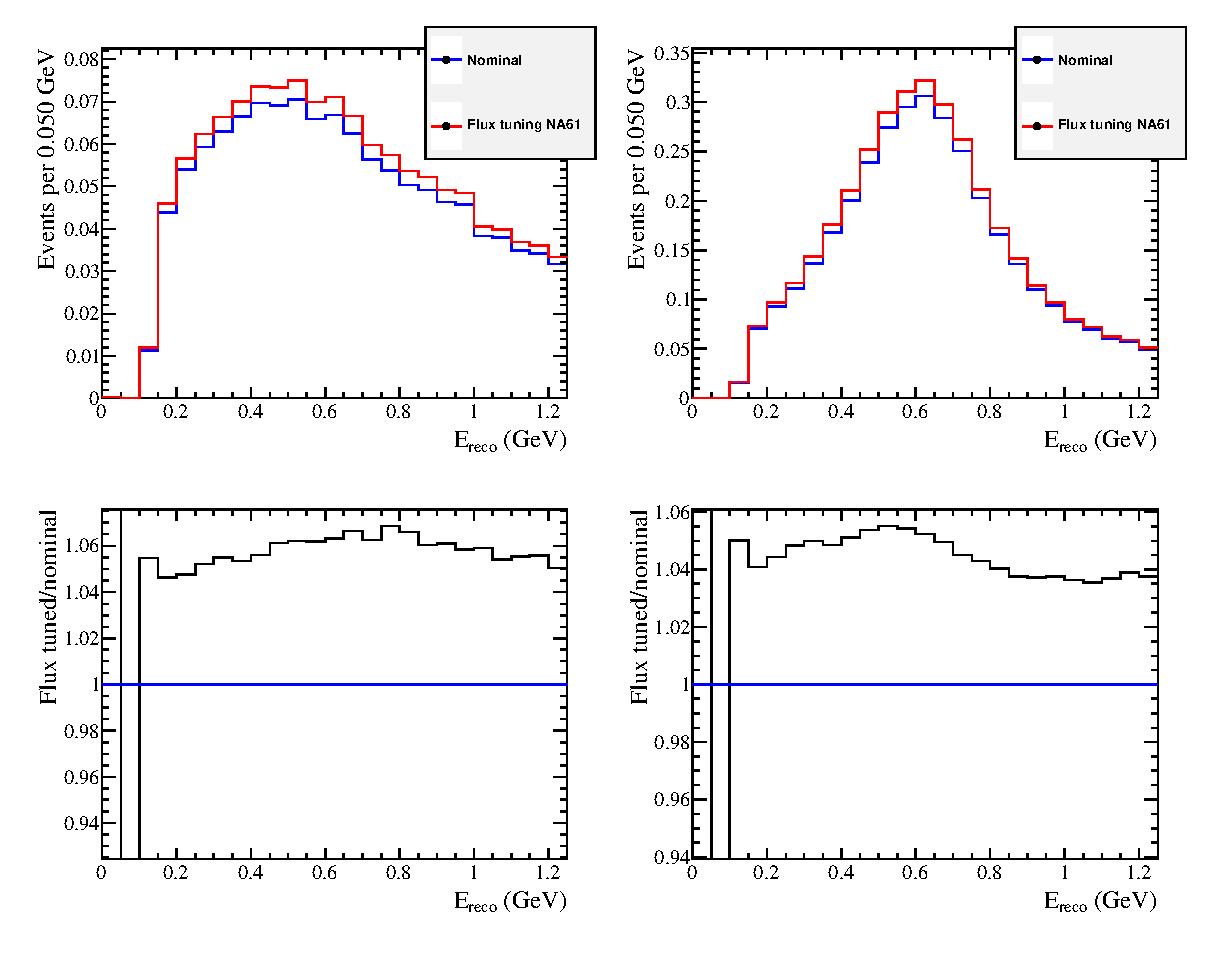
\includegraphics[width=30pc]{./nuebar_plots/spectrum_predictions/flux_tuning_effect.eps}
%\caption {
%    \huge{TO UPDATE} % caption is already ok
%{\large{SPECTRA NA61/SHINE TUNING MU-LIKE NEUTRINO MODE}}
%%Top: Reconstructed-energy spectrum of 1 $\mu$-like ring events in neutrino mode,
%%for an exposure 
%%of $6.914 \times 10^{20}$ POT %in neutrino mode
%%%and
%%%of $4.011 \times 10^{20}$ POT in antineutrino mode
%%both with and without the effect of the NA61/SHINE flux tuning of the nominal MC templates.
%%The spectra are shown both for no oscillations (left)
%%and for oscillations assuming the normal hierarchy, and the oscillation parameters shown in table~\ref{tab:osc_params_fixed_values_reactor}.
%%Bottom: Ratio of flux tuned with NA61/SHINE spectrum to the nominal MC spectrum.
%}
%\label{fig:1Rmu_spectrum_w_and_wo_na61_weights}
%\end{figure*}
%
%\begin{figure*}[htb]
%\center
%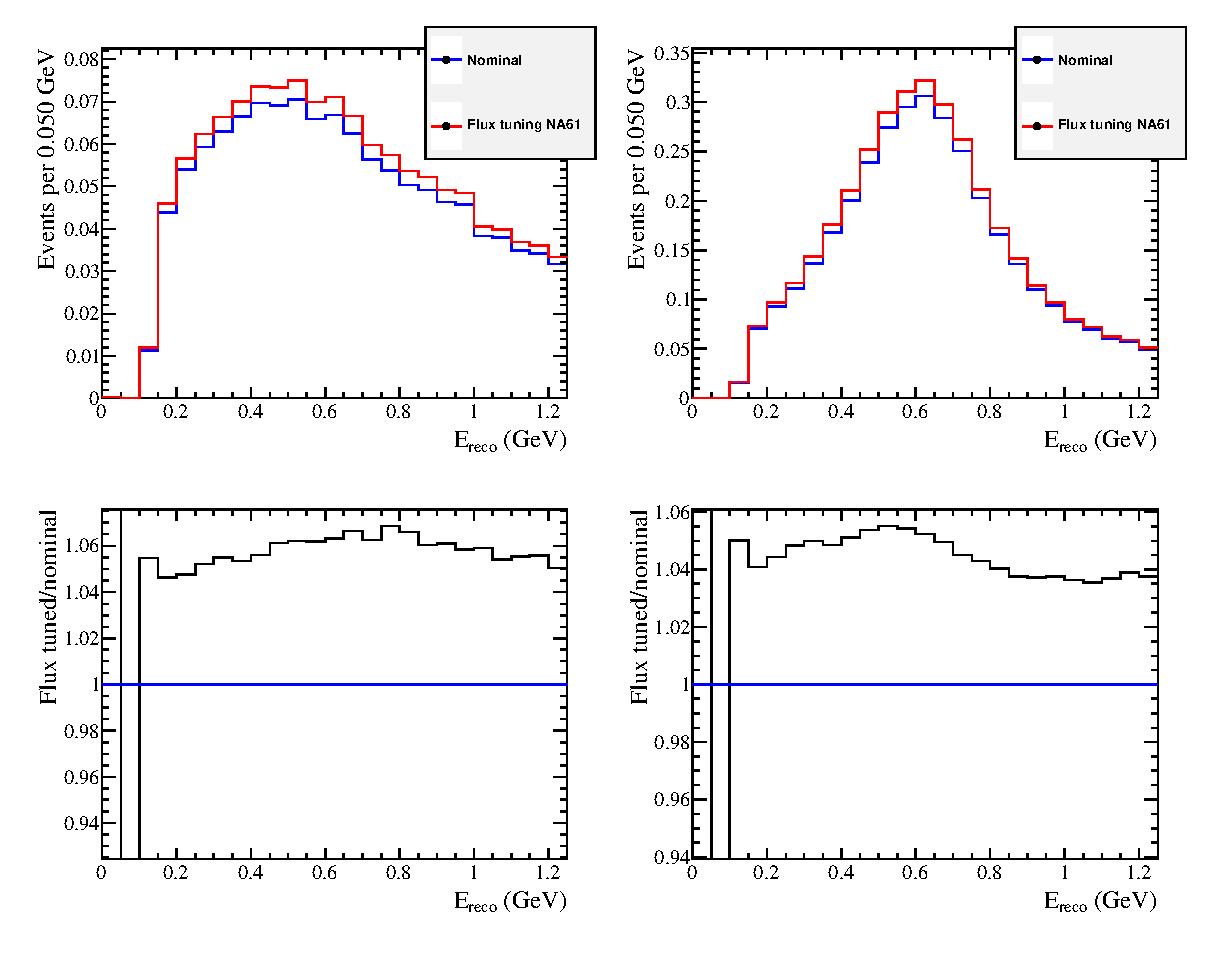
\includegraphics[width=30pc]{./nuebar_plots/spectrum_predictions/flux_tuning_effect.eps}
%\caption {
%    \huge{TO UPDATE} % caption is already ok
%{\large{SPECTRA NA61/SHINE TUNING MU-LIKE ANTINEUTRINO MODE}}
%%Top: Reconstructed-energy spectrum of 1 $\mu$-like ring events in antineutrino mode,
%%for an exposure 
%%%of $6.914 \times 10^{20}$ POT in neutrino mode
%%%and
%%of $4.011 \times 10^{20}$ POT% in antineutrino mode
%%both with and without the effect of the NA61/SHINE flux tuning of the nominal MC templates.
%%The spectra are shown both for no oscillations (left)
%%and for oscillations assuming the normal hierarchy, and the oscillation parameters shown in table~\ref{tab:osc_params_fixed_values_reactor}.
%%Bottom: Ratio of flux tuned with NA61/SHINE spectrum to the nominal MC spectrum.
%}
%\label{fig:RHC1Rmu_spectrum_w_and_wo_na61_weights}
%\end{figure*}
%
%\begin{figure*}[htb]
%\center
%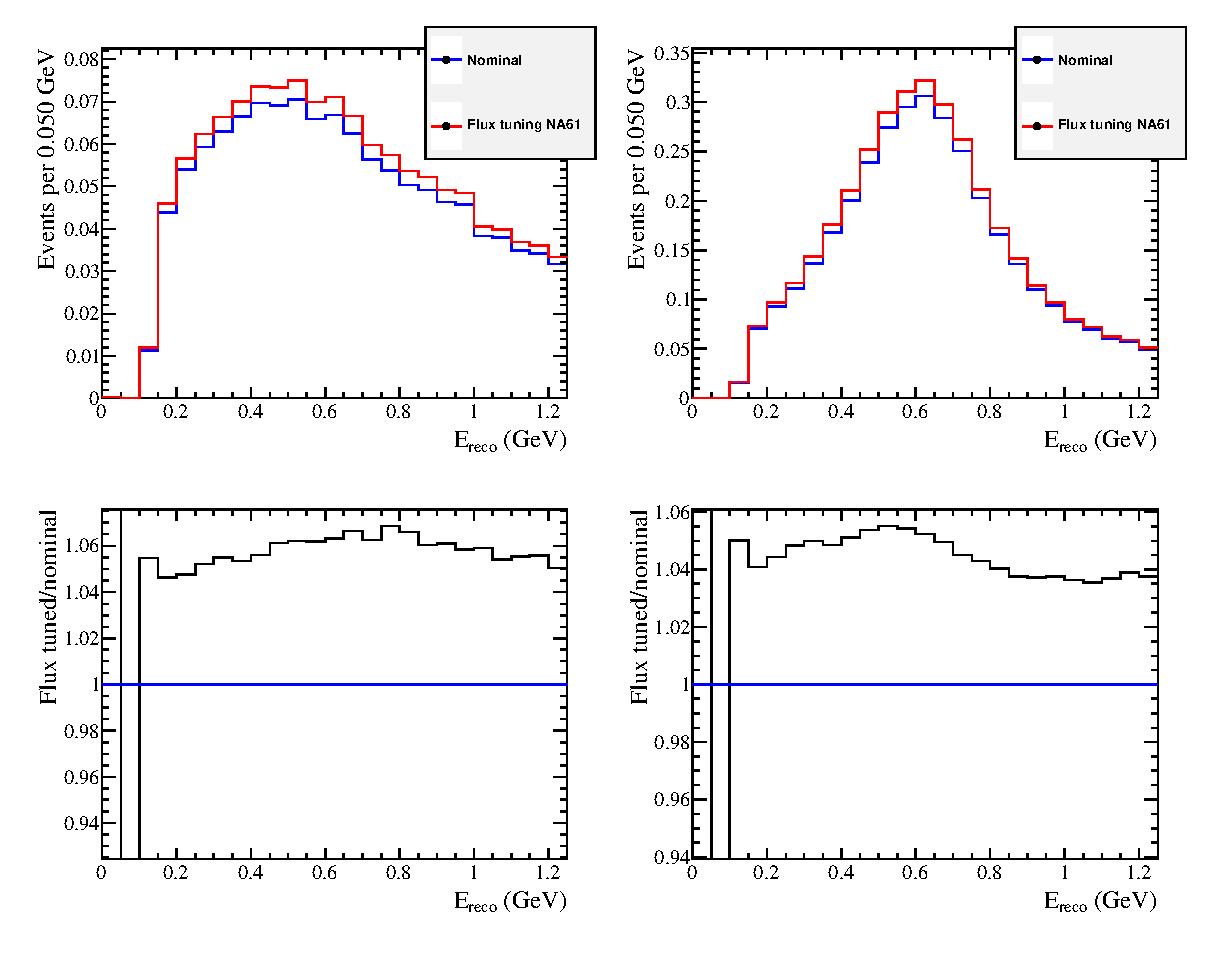
\includegraphics[width=30pc]{./nuebar_plots/spectrum_predictions/flux_tuning_effect.eps}
%\caption {
%    \huge{TO UPDATE} % caption is already ok
%{\large{SPECTRA NA61/SHINE TUNING E-LIKE NEUTRINO MODE}}
%%Top: Reconstructed-energy spectrum of 1 $e$-like ring events in neutrino mode,
%%for an exposure 
%%of $6.914 \times 10^{20}$ POT% in neutrino mode
%%%and
%%%of $4.011 \times 10^{20}$ POT in antineutrino mode
%%both with and without the effect of the NA61/SHINE flux tuning of the nominal MC templates.
%%The spectra are shown both for no oscillations (left)
%%and for oscillations assuming the normal hierarchy, and the oscillation parameters shown in table~\ref{tab:osc_params_fixed_values_reactor}.
%%Bottom: Ratio of flux tuned with NA61/SHINE spectrum to the nominal MC spectrum.
%}
%\label{fig:1Re_spectrum_w_and_wo_na61_weights}
%\end{figure*}
%
%\begin{figure*}[htb]
%\center
%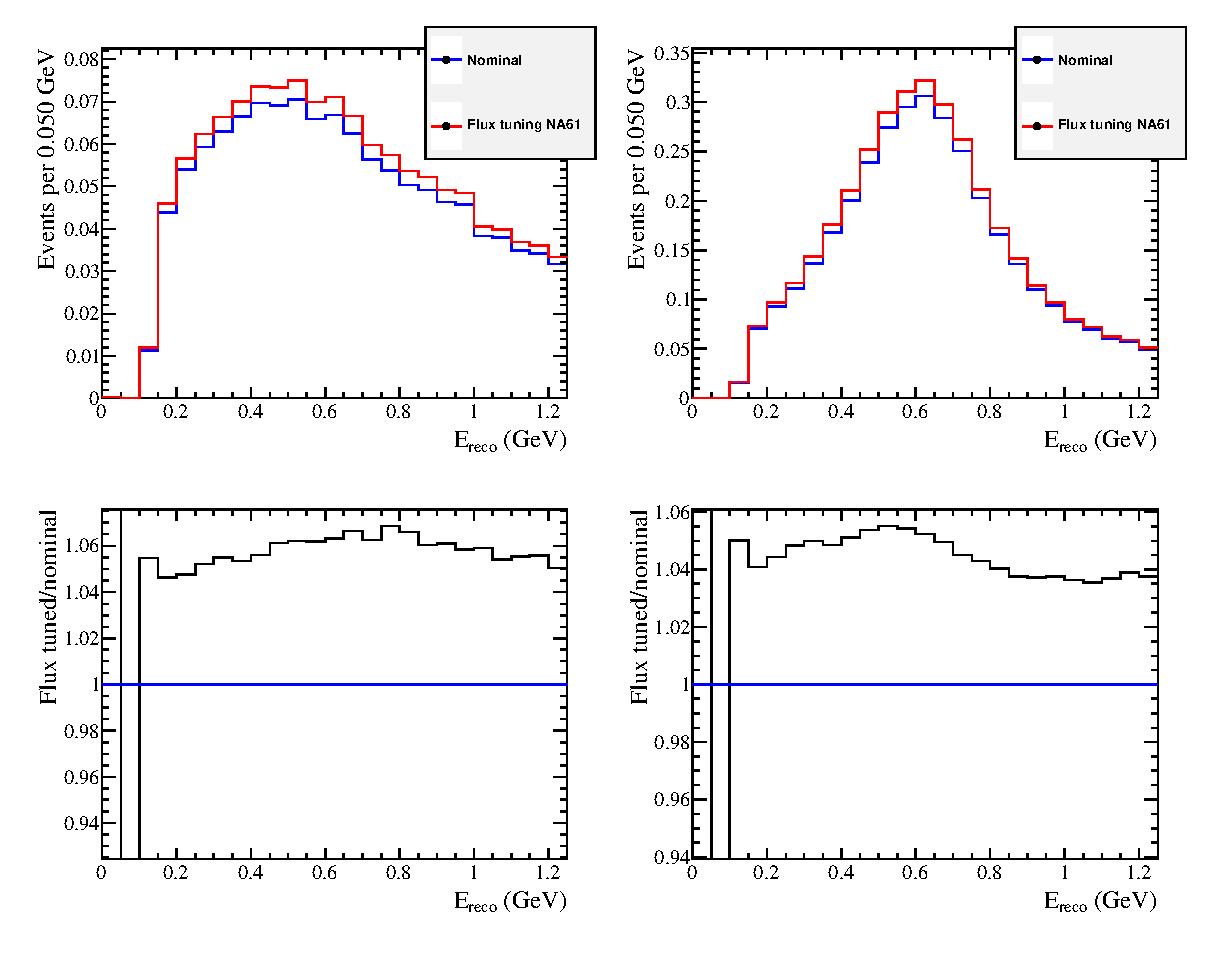
\includegraphics[width=30pc]{./nuebar_plots/spectrum_predictions/flux_tuning_effect.eps}
%\caption {
%    \huge{TO UPDATE} % caption is already ok
%{\large{SPECTRA NA61/SHINE TUNING E-LIKE ANTINEUTRINO MODE}}
%%Top: Reconstructed-energy spectrum of 1 $e$-like ring events in antineutrino mode,
%%for an exposure 
%%%of $6.914 \times 10^{20}$ POT in neutrino mode
%%%and
%%of $4.011 \times 10^{20}$ POT %in antineutrino mode
%%both with and without the effect of the NA61/SHINE flux tuning of the nominal MC templates.
%%The spectra are shown both for no oscillations (left)
%%and for oscillations assuming the normal hierarchy, and the oscillation parameters shown in table~\ref{tab:osc_params_fixed_values_reactor}.
%%Bottom: Ratio of flux tuned with NA61/SHINE spectrum to the nominal MC spectrum.
%}
%\label{fig:RHC1Re_spectrum_w_and_wo_na61_weights}
%\end{figure*}
%
%
%
%
%
%
%
%
%
%
%% Plots showing the effect of tunes on Ereco spectra w/ and w/o BANFF
%
%\begin{figure*}[htb]
%\center
%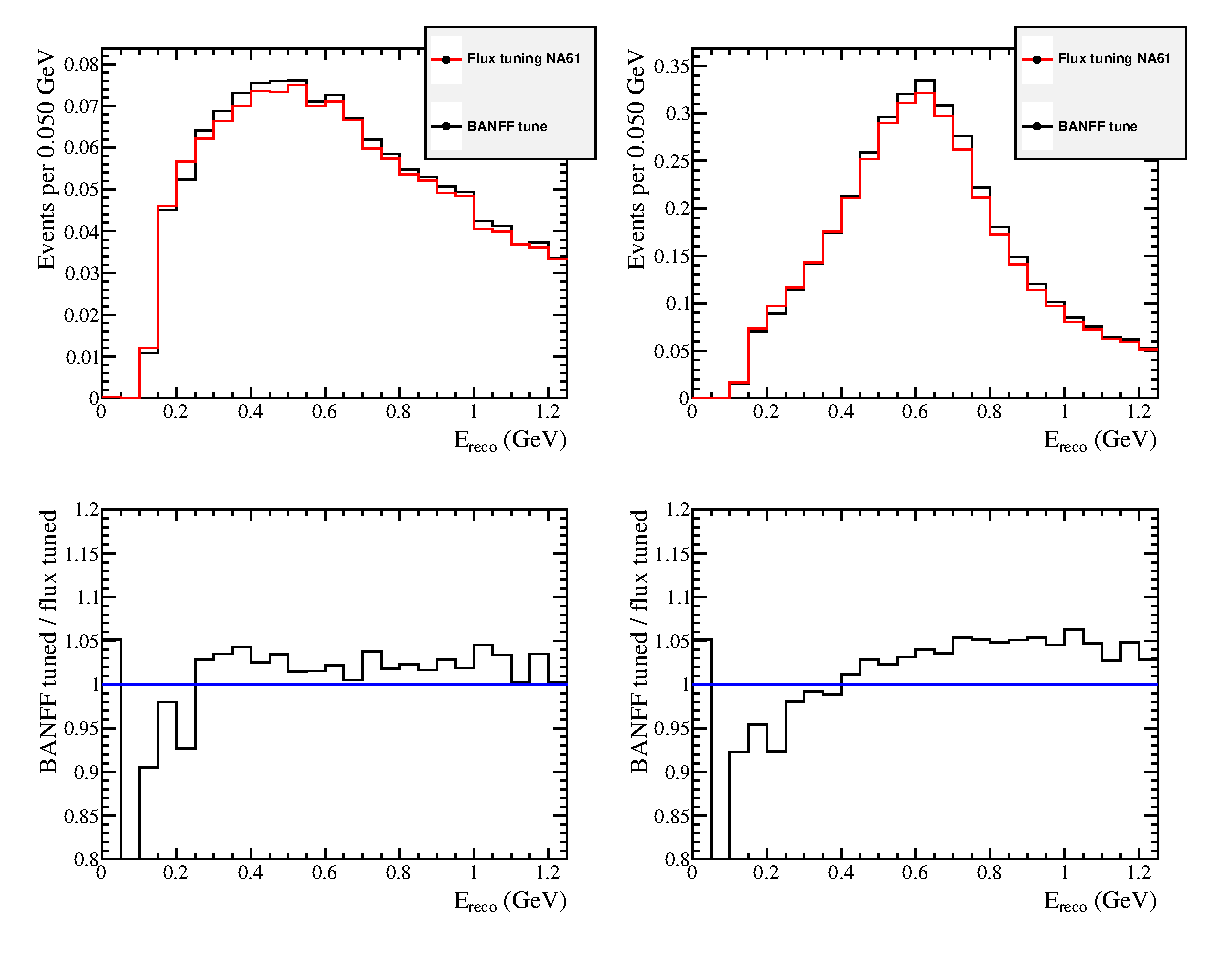
\includegraphics[width=30pc]{./nuebar_plots/spectrum_predictions/banff_tuning_effect.eps}
%\caption {
%    \huge{TO UPDATE} % caption is already ok
%{\large{SPECTRA BANFF TUNING MU-LIKE NEUTRINO MODE}}
%%Top: Reconstructed-energy spectrum of 1 $\mu$-like ring events in neutrino mode,
%%for an exposure 
%%of $6.914 \times 10^{20}$ POT % in neutrino mode
%%%and
%%%of $4.011 \times 10^{20}$ POT in antineutrino mode
%%both with and without the effect of postfit BANFF flux and cross-section tuning on the NA61/SHINE-tuned flux MC templates.
%%The spectra are shown both for no oscillations (left)
%%and for oscillations assuming the normal hierarchy, and the oscillation parameters shown in table~\ref{tab:osc_params_fixed_values_reactor}.
%%Bottom: Ratio of BANFF-tuned spectrum to the flux tuned with NA61/SHINE spectrum.
%}
%\label{fig:1Rmu_spectrum_w_and_wo_banff_weights}
%\end{figure*}
%
%\begin{figure*}[htb]
%\center
%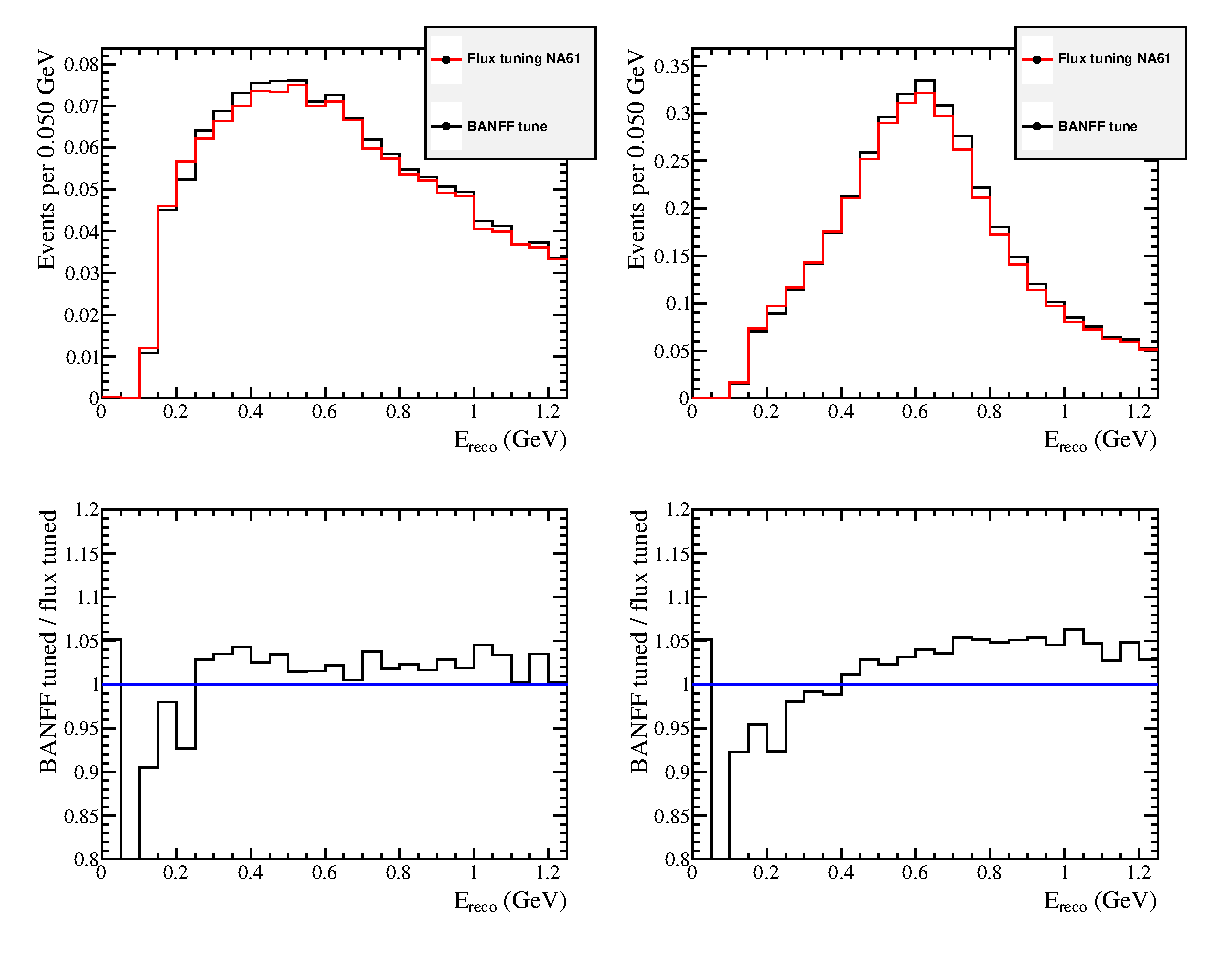
\includegraphics[width=30pc]{./nuebar_plots/spectrum_predictions/banff_tuning_effect.eps}
%\caption {
%    \huge{TO UPDATE} % caption is already ok
%{\large{SPECTRA BANFF TUNING MU-LIKE ANTINEUTRINO MODE}}
%%Top: Reconstructed-energy spectrum of 1 $\mu$-like ring events in antineutrino mode,
%%for an exposure 
%%%of $6.914 \times 10^{20}$ POT in neutrino mode
%%%and
%%of $4.011 \times 10^{20}$ POT% in antineutrino mode
%%both with and without the effect of postfit BANFF flux and cross-section tuning on the NA61/SHINE-tuned flux MC templates.
%%The spectra are shown both for no oscillations (left)
%%and for oscillations assuming the normal hierarchy, and the oscillation parameters shown in table~\ref{tab:osc_params_fixed_values_reactor}.
%%Bottom: Ratio of BANFF-tuned spectrum to the flux tuned with NA61/SHINE spectrum.
%}
%\label{fig:RHC1Rmu_spectrum_w_and_wo_banff_weights}
%\end{figure*}
%
%\begin{figure*}[htb]
%\center
%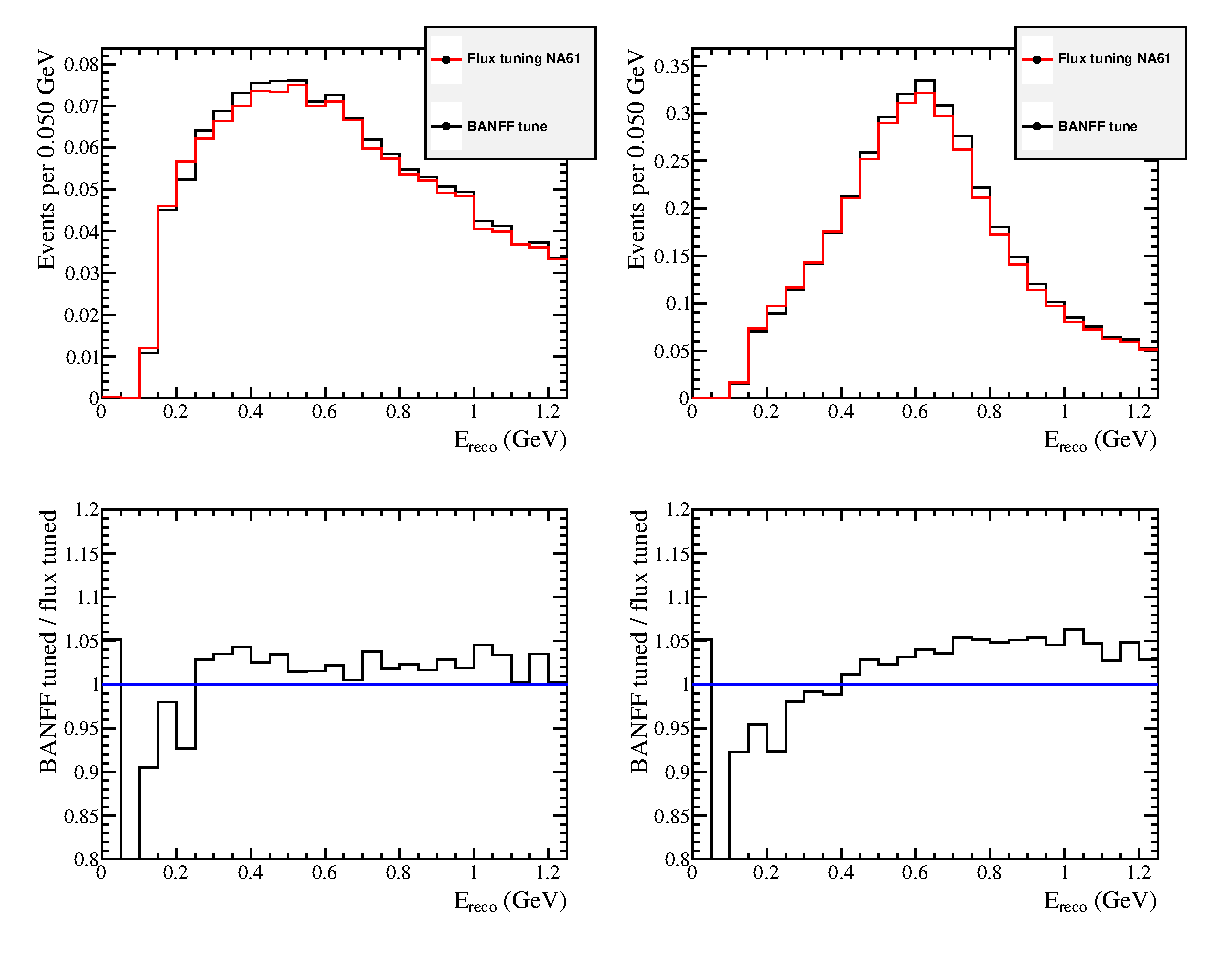
\includegraphics[width=30pc]{./nuebar_plots/spectrum_predictions/banff_tuning_effect.eps}
%\caption {
%    \huge{TO UPDATE} % caption is already ok
%{\large{SPECTRA BANFF TUNING E-LIKE NEUTRINO MODE}}
%%Top: Reconstructed-energy spectrum of 1 $e$-like ring events in neutrino mode,
%%for an exposure 
%%of $6.914 \times 10^{20}$ POT %in neutrino mode
%%%and
%%%of $4.011 \times 10^{20}$ POT in antineutrino mode
%%both with and without the effect of postfit BANFF flux and cross-section tuning on the NA61/SHINE-tuned flux MC templates.
%%The spectra are shown both for no oscillations (left)
%%and for oscillations assuming the normal hierarchy, and the oscillation parameters shown in table~\ref{tab:osc_params_fixed_values_reactor}.
%%Bottom: Ratio of BANFF-tuned spectrum to the flux tuned with NA61/SHINE spectrum.
%}
%\label{fig:1Re_spectrum_w_and_wo_banff_weights}
%\end{figure*}
%
%\begin{figure*}[htb]
%\center
%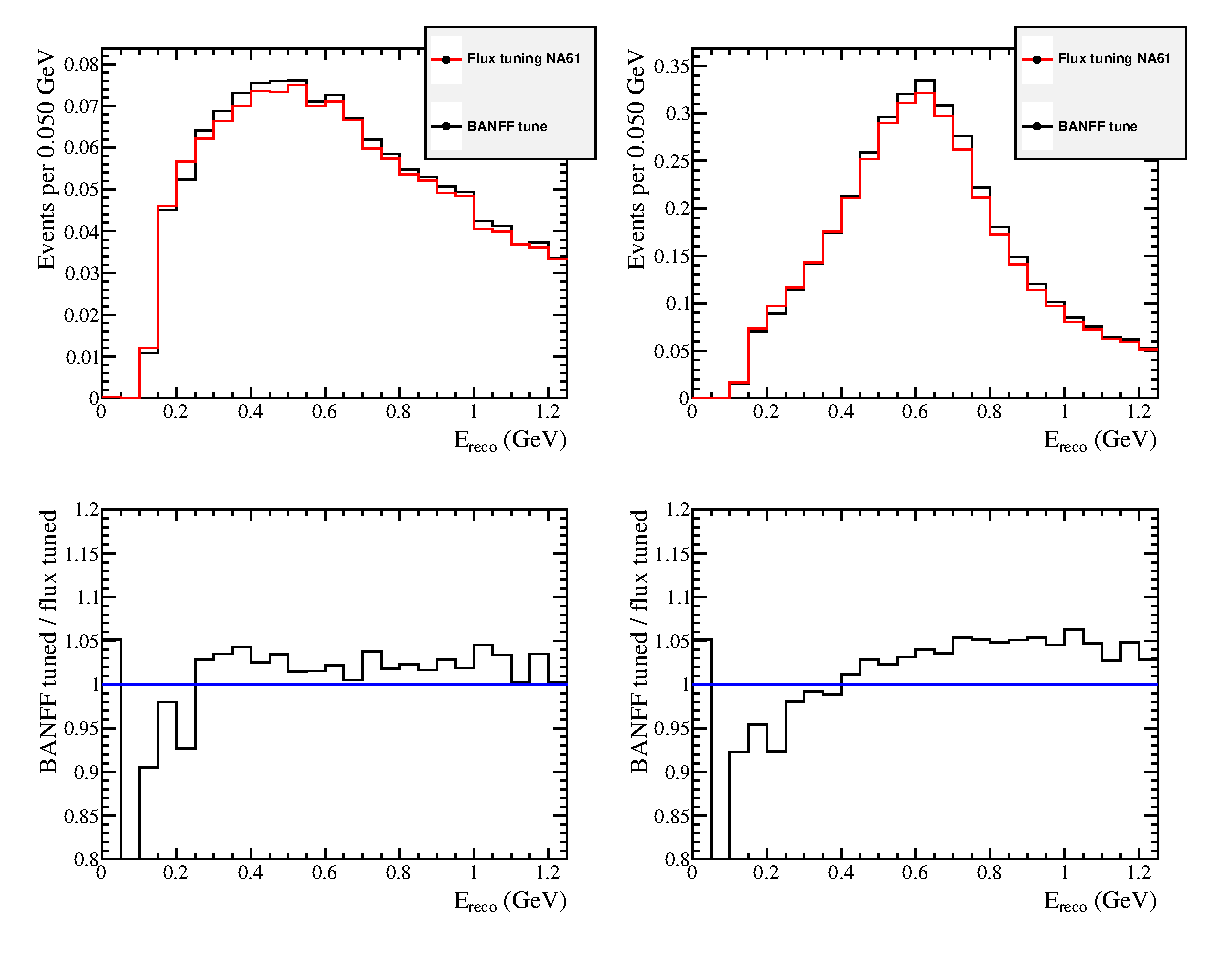
\includegraphics[width=30pc]{./nuebar_plots/spectrum_predictions/banff_tuning_effect.eps}
%\caption {
%    \huge{TO UPDATE} % caption is already ok
%{\large{SPECTRA BANFF TUNING E-LIKE ANTINEUTRINO MODE}}
%%Top: Reconstructed-energy spectrum of 1 $e$-like ring events in antineutrino mode,
%%for an exposure 
%%%of $6.914 \times 10^{20}$ POT in neutrino mode
%%%and
%%of $4.011 \times 10^{20}$ POT %in antineutrino mode
%%both with and without the effect of postfit BANFF flux and cross-section tuning on the NA61/SHINE-tuned flux MC templates.
%%The spectra are shown both for no oscillations (left)
%%and for oscillations assuming the normal hierarchy, and the oscillation parameters shown in table~\ref{tab:osc_params_fixed_values_reactor}.
%%Bottom: Ratio of BANFF-tuned spectrum to the flux tuned with NA61/SHINE spectrum.
%}
%\label{fig:RHC1Re_spectrum_w_and_wo_banff_weights}
%\end{figure*}
%
%\newpage
%\clearpage

In \cref{tab:events_1rmu_Asimov_B},
\ref{tab:events_rhc1rmu_Asimov_B} and
\ref{tab:events_1re_Asimov_B},
\ref{tab:events_rhc1re_Asimov_B} 
the total number of events expected for the Asimov data set B (see \cref{tab:osc_params_joint_asimov}) is shown.

%\newpage
\clearpage


\begin{table}
\center
\begin{tabular} { | l ||r | r | r | r | r | r | | r | }
\hline
              & $\nu_\mu$            & $\nu_e$              & $\bar{\nu_\mu}$      & $\bar{\nu_e}$        & Osc. $\nu_e$         & Osc. $\bar{\nu_e}$   & Total                \\ \hline\hline
 CCQE         & 69.747               & 0.035                & 4.335                & 0.002                & 0.151                & 0.001                & 74.270               \\ \hline
 CC1pi        & 17.206               & 0.017                & 1.572                & 0.001                & 0.049                & 0.000                & 18.845               \\ \hline
 CCcoherent   & 0.330                & 0.000                & 0.080                & 0.000                & 0.001                & 0.000                & 0.412                \\ \hline
 2p-2h          & 19.725               & 0.010                & 0.852                & 0.000                & 0.036                & 0.000                & 20.623               \\ \hline
 CCother      & 7.742                & 0.008                & 0.494                & 0.001                & 0.002                & 0.000                & 8.247                \\ \hline
 NC1pi0       & 0.537                & 0.016                & 0.017                & 0.001                & N/A                  & N/A                  & 0.572                \\ \hline
 NC1piPM      & 3.944                & 0.089                & 0.142                & 0.008                & N/A                  & N/A                  & 4.183                \\ \hline
 NCcoherent   & 0.016                & 0.000                & 0.001                & 0.000                & N/A                  & N/A                  & 0.018                \\ \hline
 NCother      & 2.993                & 0.121                & 0.165                & 0.012                & N/A                  & N/A                  & 3.290                \\ \hline
 NC1gamma     & 0.004                & 0.000                & 0.000                & 0.000                & N/A                  & N/A                  & 0.004                \\ \hline
\hline
 Total        & 122.243              & 0.297                & 7.659                & 0.025                & 0.238                & 0.002                & 130.464              \\ \hline
\end{tabular}
\caption{
%{\Huge{TO UPDATE}}
Predicted number of events in the neutrino mode $\mu$-like sample
obtained after applying the BANFF weight
for a total exposure of \TotalPotNu{} POT.
The Asimov data set B in \cref{tab:osc_params_joint_asimov} is used.
}
\label{tab:events_1rmu_Asimov_B}
\end{table}




\begin{table}
\center
\begin{tabular} { | l ||r | r | r | r | r | r | | r | }
\hline
             & $\nu_\mu$            & $\nu_e$              & $\bar{\nu_\mu}$      & $\bar{\nu_e}$        & Osc. $\nu_e$         & Osc. $\bar{\nu_e}$   & Total                \\ \hline\hline
 CCQE         & 7.088                & 0.004                & 13.306               & 0.005                & 0.004                & 0.016                & 20.422               \\ \hline
 CC1pi        & 2.718                & 0.003                & 3.066                & 0.002                & 0.002                & 0.003                & 5.794                \\ \hline
 CCcoherent   & 0.054                & 0.000                & 0.173                & 0.000                & 0.000                & 0.000                & 0.228                \\ \hline
 2p-2h          & 2.525                & 0.001                & 2.118                & 0.001                & 0.001                & 0.002                & 4.649                \\ \hline
 CCother      & 1.282                & 0.001                & 0.886                & 0.000                & 0.000                & 0.000                & 2.170                \\ \hline
 NC1pi0       & 0.060                & 0.002                & 0.050                & 0.001                & N/A                  & N/A                  & 0.114                \\ \hline
 NC1piPM      & 0.378                & 0.015                & 0.380                & 0.010                & N/A                  & N/A                  & 0.784                \\ \hline
 NCcoherent   & 0.001                & 0.000                & 0.006                & 0.000                & N/A                  & N/A                  & 0.008                \\ \hline
 NCother      & 0.530                & 0.025                & 0.296                & 0.012                & N/A                  & N/A                  & 0.862                \\ \hline
 NC1gamma     & 0.000                & 0.000                & 0.000                & 0.000                & N/A                  & N/A                  & 0.000                \\ \hline
\hline
 Total        & 14.637               & 0.051                & 20.282               & 0.032                & 0.008                & 0.022                & 35.032               \\ \hline

\end{tabular}
\caption{
%{\Huge{TO UPDATE}}
Predicted number of events in the antineutrino mode $\mu$-like sample
obtained after applying the BANFF weight
for a total exposure of \TotalPotNuBar{} POT.
The Asimov data set B in \cref{tab:osc_params_joint_asimov} is used.
}
\label{tab:events_rhc1rmu_Asimov_B}
\end{table}




\begin{table}
\center
\begin{tabular} { | l ||r | r | r | r | r | r | | r | }
\hline
              & $\nu_\mu$            & $\nu_e$              & $\bar{\nu_\mu}$      & $\bar{\nu_e}$        & Osc. $\nu_e$         & Osc. $\bar{\nu_e}$   & Total                \\ \hline\hline
 CCQE         & 0.062                & 2.129                & 0.001                & 0.088                & 10.811               & 0.121                & 13.211               \\ \hline
 CC1pi        & 0.017                & 0.348                & 0.000                & 0.027                & 1.236                & 0.020                & 1.648                \\ \hline
 CCcoherent   & 0.000                & 0.002                & 0.000                & 0.002                & 0.011                & 0.002                & 0.017                \\ \hline
 2p-2h          & 0.009                & 0.710                & 0.000                & 0.022                & 2.750                & 0.022                & 3.513                \\ \hline
 CCother      & 0.001                & 0.045                & 0.000                & 0.003                & 0.025                & 0.001                & 0.076                \\ \hline
 NC1pi0       & 0.524                & 0.012                & 0.017                & 0.001                & N/A                  & N/A                  & 0.553                \\ \hline
 NC1piPM      & 0.099                & 0.002                & 0.003                & 0.000                & N/A                  & N/A                  & 0.105                \\ \hline
 NCcoherent   & 0.174                & 0.004                & 0.018                & 0.001                & N/A                  & N/A                  & 0.197                \\ \hline
 NCother      & 0.126                & 0.005                & 0.008                & 0.001                & N/A                  & N/A                  & 0.139                \\ \hline
 NC1gamma     & 0.464                & 0.007                & 0.021                & 0.001                & N/A                  & N/A                  & 0.494                \\ \hline
\hline
 Total        & 1.476                & 3.264                & 0.069                & 0.145                & 14.833               & 0.167                & 19.954               \\ \hline

\end{tabular}
\caption{
%{\Huge{TO UPDATE}}
Predicted number of events in the neutrino mode $e$-like sample
obtained after applying the BANFF weight
for a total exposure of \TotalPotNu{} POT.
The Asimov data set B in \cref{tab:osc_params_joint_asimov} is used.
}
\label{tab:events_1re_Asimov_B}
\end{table}




\begin{table}
\center
\begin{tabular} { | l ||r | r | r | r | r | r | | r | }
\hline
              & $\nu_\mu$            & $\nu_e$              & $\bar{\nu_\mu}$      & $\bar{\nu_e}$        & Osc. $\nu_e$         & Osc. $\bar{\nu_e}$   & Total                \\ \hline\hline
 CCQE         & 0.002                & 0.189                & 0.003                & 0.339                & 0.269                & 1.376                & 2.178                \\ \hline
 CC1pi        & 0.002                & 0.040                & 0.001                & 0.060                & 0.045                & 0.163                & 0.312                \\ \hline
 CCcoherent   & 0.000                & 0.000                & 0.000                & 0.006                & 0.000                & 0.022                & 0.029                \\ \hline
 2p-2h          & 0.001                & 0.069                & 0.000                & 0.063                & 0.087                & 0.219                & 0.439                \\ \hline
 CCother      & 0.001                & 0.008                & 0.000                & 0.004                & 0.003                & 0.003                & 0.019                \\ \hline
 NC1pi0       & 0.045                & 0.002                & 0.049                & 0.001                & N/A                  & N/A                  & 0.098                \\ \hline
 NC1piPM      & 0.011                & 0.000                & 0.008                & 0.000                & N/A                  & N/A                  & 0.020                \\ \hline
 NCcoherent   & 0.021                & 0.001                & 0.081                & 0.001                & N/A                  & N/A                  & 0.103                \\ \hline
 NCother      & 0.022                & 0.001                & 0.012                & 0.000                & N/A                  & N/A                  & 0.035                \\ \hline
 NC1gamma     & 0.037                & 0.002                & 0.081                & 0.002                & N/A                  & N/A                  & 0.121                \\ \hline
\hline
 Total        & 0.142                & 0.313                & 0.235                & 0.478                & 0.404                & 1.783                & 3.355                \\ \hline

\end{tabular}
\caption{
%{\Huge{TO UPDATE}}
Predicted number of events in the antineutrino mode $\mu$-like sample
obtained after applying the BANFF weight
for a total exposure of \TotalPotNuBar{} POT.
The Asimov data set B in \cref{tab:osc_params_joint_asimov} is used.
}
\label{tab:events_rhc1re_Asimov_B}
\end{table}





\newpage
\clearpage

In \cref{tab:events_1rmu_NoOsc},
\ref{tab:events_rhc1rmu_NoOsc} and
\ref{tab:events_1re_NoOsc},
\ref{tab:events_rhc1re_NoOsc}
the total number of unoscillated events is shown.
 

\begin{table}
\center
\begin{tabular} { | l ||r | r | r | r | r | r | | r | }
\hline
              & $\nu_\mu$            & $\nu_e$              & $\bar{\nu_\mu}$      & $\bar{\nu_e}$        & Osc. $\nu_e$         & Osc. $\bar{\nu_e}$   & Total                \\ \hline\hline
 CCQE         & 338.683              & 0.037                & 8.672                & 0.002                & 0.000                & 0.000                & 347.394              \\ \hline
 CC1pi        & 39.668               & 0.018                & 2.276                & 0.001                & 0.000                & 0.000                & 41.963               \\ \hline
 CCcoherent   & 0.678                & 0.000                & 0.136                & 0.000                & 0.000                & 0.000                & 0.815                \\ \hline
 2p-2h          & 74.638               & 0.011                & 1.548                & 0.000                & 0.000                & 0.000                & 76.198               \\ \hline
 CCother      & 8.732                & 0.009                & 0.560                & 0.001                & 0.000                & 0.000                & 9.301                \\ \hline
 NC1pi0       & 0.537                & 0.016                & 0.017                & 0.001                & N/A                  & N/A                  & 0.572                \\ \hline
 NC1piPM      & 3.944                & 0.089                & 0.142                & 0.008                & N/A                  & N/A                  & 4.183                \\ \hline
 NCcoherent   & 0.016                & 0.000                & 0.001                & 0.000                & N/A                  & N/A                  & 0.018                \\ \hline
 NCother      & 2.993                & 0.121                & 0.165                & 0.012                & N/A                  & N/A                  & 3.290                \\ \hline
 NC1gamma     & 0.004                & 0.000                & 0.000                & 0.000                & N/A                  & N/A                  & 0.004                \\ \hline
\hline
 Total        & 469.893              & 0.301                & 13.518               & 0.025                & 0.000                & 0.000                & 483.737              \\ \hline
\end{tabular}
\caption{
%{\Huge{TO UPDATE}}
Predicted number of events in the neutrino mode $\mu$-like sample
obtained after applying the BANFF weight
for a total exposure of \TotalPotNu{} POT.
Oscillations are not applied.
}
\label{tab:events_1rmu_NoOsc}
\end{table}




\begin{table}
\center
\begin{tabular} { | l ||r | r | r | r | r | r | | r | }
\hline
              & $\nu_\mu$            & $\nu_e$              & $\bar{\nu_\mu}$      & $\bar{\nu_e}$        & Osc. $\nu_e$         & Osc. $\bar{\nu_e}$   & Total                \\ \hline\hline
 CCQE         & 15.420               & 0.004                & 55.525               & 0.005                & 0.000                & 0.000                & 70.954               \\ \hline
 CC1pi        & 4.071                & 0.003                & 6.536                & 0.002                & 0.000                & 0.000                & 10.611               \\ \hline
 CCcoherent   & 0.074                & 0.000                & 0.612                & 0.000                & 0.000                & 0.000                & 0.687                \\ \hline
 2p-2h          & 4.721                & 0.001                & 7.811                & 0.001                & 0.000                & 0.000                & 12.534               \\ \hline
 CCother      & 1.457                & 0.001                & 1.008                & 0.000                & 0.000                & 0.000                & 2.467                \\ \hline
 NC1pi0       & 0.060                & 0.002                & 0.050                & 0.001                & N/A                  & N/A                  & 0.114                \\ \hline
 NC1piPM      & 0.378                & 0.015                & 0.380                & 0.010                & N/A                  & N/A                  & 0.784                \\ \hline
 NCcoherent   & 0.001                & 0.000                & 0.006                & 0.000                & N/A                  & N/A                  & 0.008                \\ \hline
 NCother      & 0.530                & 0.025                & 0.296                & 0.012                & N/A                  & N/A                  & 0.862                \\ \hline
 NC1gamma     & 0.000                & 0.000                & 0.000                & 0.000                & N/A                  & N/A                  & 0.000                \\ \hline
\hline
 Total        & 26.713               & 0.052                & 72.225               & 0.032                & 0.000                & 0.000                & 99.021               \\ \hline

\end{tabular}
\caption{
%{\Huge{TO UPDATE}}
Predicted number of events in the antineutrino mode $\mu$-like sample
obtained after applying the BANFF weight
for a total exposure of \TotalPotNuBar{} POT.
Oscillations are not applied.
}
\label{tab:events_rhc1rmu_NoOsc}
\end{table}




\begin{table}
\center
\begin{tabular} { | l ||r | r | r | r | r | r | | r | }
\hline
               & $\nu_\mu$            & $\nu_e$              & $\bar{\nu_\mu}$      & $\bar{\nu_e}$        & Osc. $\nu_e$         & Osc. $\bar{\nu_e}$   & Total                \\ \hline\hline
 CCQE         & 0.413                & 2.294                & 0.002                & 0.094                & 0.000                & 0.000                & 2.803                \\ \hline
 CC1pi        & 0.069                & 0.371                & 0.001                & 0.028                & 0.000                & 0.000                & 0.469                \\ \hline
 CCcoherent   & 0.002                & 0.003                & 0.000                & 0.002                & 0.000                & 0.000                & 0.006                \\ \hline
 2p-2h          & 0.095                & 0.759                & 0.000                & 0.023                & 0.000                & 0.000                & 0.878                \\ \hline
 CCother      & 0.004                & 0.046                & 0.000                & 0.003                & 0.000                & 0.000                & 0.054                \\ \hline
 NC1pi0       & 0.524                & 0.012                & 0.017                & 0.001                & N/A                  & N/A                  & 0.553                \\ \hline
 NC1piPM      & 0.099                & 0.002                & 0.003                & 0.000                & N/A                  & N/A                  & 0.105                \\ \hline
 NCcoherent   & 0.174                & 0.004                & 0.018                & 0.001                & N/A                  & N/A                  & 0.197                \\ \hline
 NCother      & 0.126                & 0.005                & 0.008                & 0.001                & N/A                  & N/A                  & 0.139                \\ \hline
 NC1gamma     & 0.464                & 0.007                & 0.021                & 0.001                & N/A                  & N/A                  & 0.494                \\ \hline
\hline
 Total        & 1.970                & 3.504                & 0.071                & 0.154                & 0.000                & 0.000                & 5.698                \\ \hline

\end{tabular}
\caption{
%{\Huge{TO UPDATE}}
Predicted number of events in the neutrino mode $e$-like sample
obtained after applying the BANFF weight
for a total exposure of \TotalPotNu{} POT.
Oscillations are not applied.
}
\label{tab:events_1re_NoOsc}
\end{table}




\begin{table}
\center
\begin{tabular} { | l ||r | r | r | r | r | r | | r | }
\hline
              & $\nu_\mu$            & $\nu_e$              & $\bar{\nu_\mu}$      & $\bar{\nu_e}$        & Osc. $\nu_e$         & Osc. $\bar{\nu_e}$   & Total                \\ \hline\hline
 CCQE         & 0.012                & 0.203                & 0.018                & 0.361                & 0.000                & 0.000                & 0.593                \\ \hline
 CC1pi        & 0.004                & 0.043                & 0.003                & 0.064                & 0.000                & 0.000                & 0.114                \\ \hline
 CCcoherent   & 0.000                & 0.000                & 0.000                & 0.006                & 0.000                & 0.000                & 0.007                \\ \hline
 2p-2h          & 0.003                & 0.074                & 0.003                & 0.067                & 0.000                & 0.000                & 0.147                \\ \hline
 CCother      & 0.001                & 0.009                & 0.000                & 0.004                & 0.000                & 0.000                & 0.015                \\ \hline
 NC1pi0       & 0.045                & 0.002                & 0.049                & 0.001                & N/A                  & N/A                  & 0.098                \\ \hline
 NC1piPM      & 0.011                & 0.000                & 0.008                & 0.000                & N/A                  & N/A                  & 0.020                \\ \hline
 NCcoherent   & 0.021                & 0.001                & 0.081                & 0.001                & N/A                  & N/A                  & 0.103                \\ \hline
 NCother      & 0.022                & 0.001                & 0.012                & 0.000                & N/A                  & N/A                  & 0.035                \\ \hline
 NC1gamma     & 0.037                & 0.002                & 0.081                & 0.002                & N/A                  & N/A                  & 0.121                \\ \hline
\hline
 Total        & 0.156                & 0.334                & 0.255                & 0.507                & 0.000                & 0.000                & 1.253                \\ \hline

\end{tabular}
\caption{
%{\Huge{TO UPDATE}}
Predicted number of events in the antineutrino mode $e$-like sample
obtained after applying the BANFF weight
for a total exposure of \TotalPotNuBar{} POT.
Oscillations are not applied.
}
\label{tab:events_rhc1re_NoOsc}
\end{table}





\clearpage






%
%...........................................................
%
% Predicted spectra
%
%...........................................................

\section{Predicted $e$-like spectra}
\label{app:templates_elike}

In \cref{fig:joint_ereco_components} each flavor component 
of the neutrino and antineutrino mode $e$-like samples
is shown separately in order to compare the different shapes as a function of $E_{reco}$.
The NC spectrum distribution,
which is the largest component of the background,
is quite flat over all the energy range and is quite difficult to separate.
The $\nu_{\mu} \rightarrow \nu_e$ and $\bar{\nu}_{\mu} \rightarrow \bar{\nu}_e$ events
populate the same energy region, around 0.6 GeV, with a very similar shape.

\begin{figure*}[htb]
%\hspace{0.06\linewidth}
\center
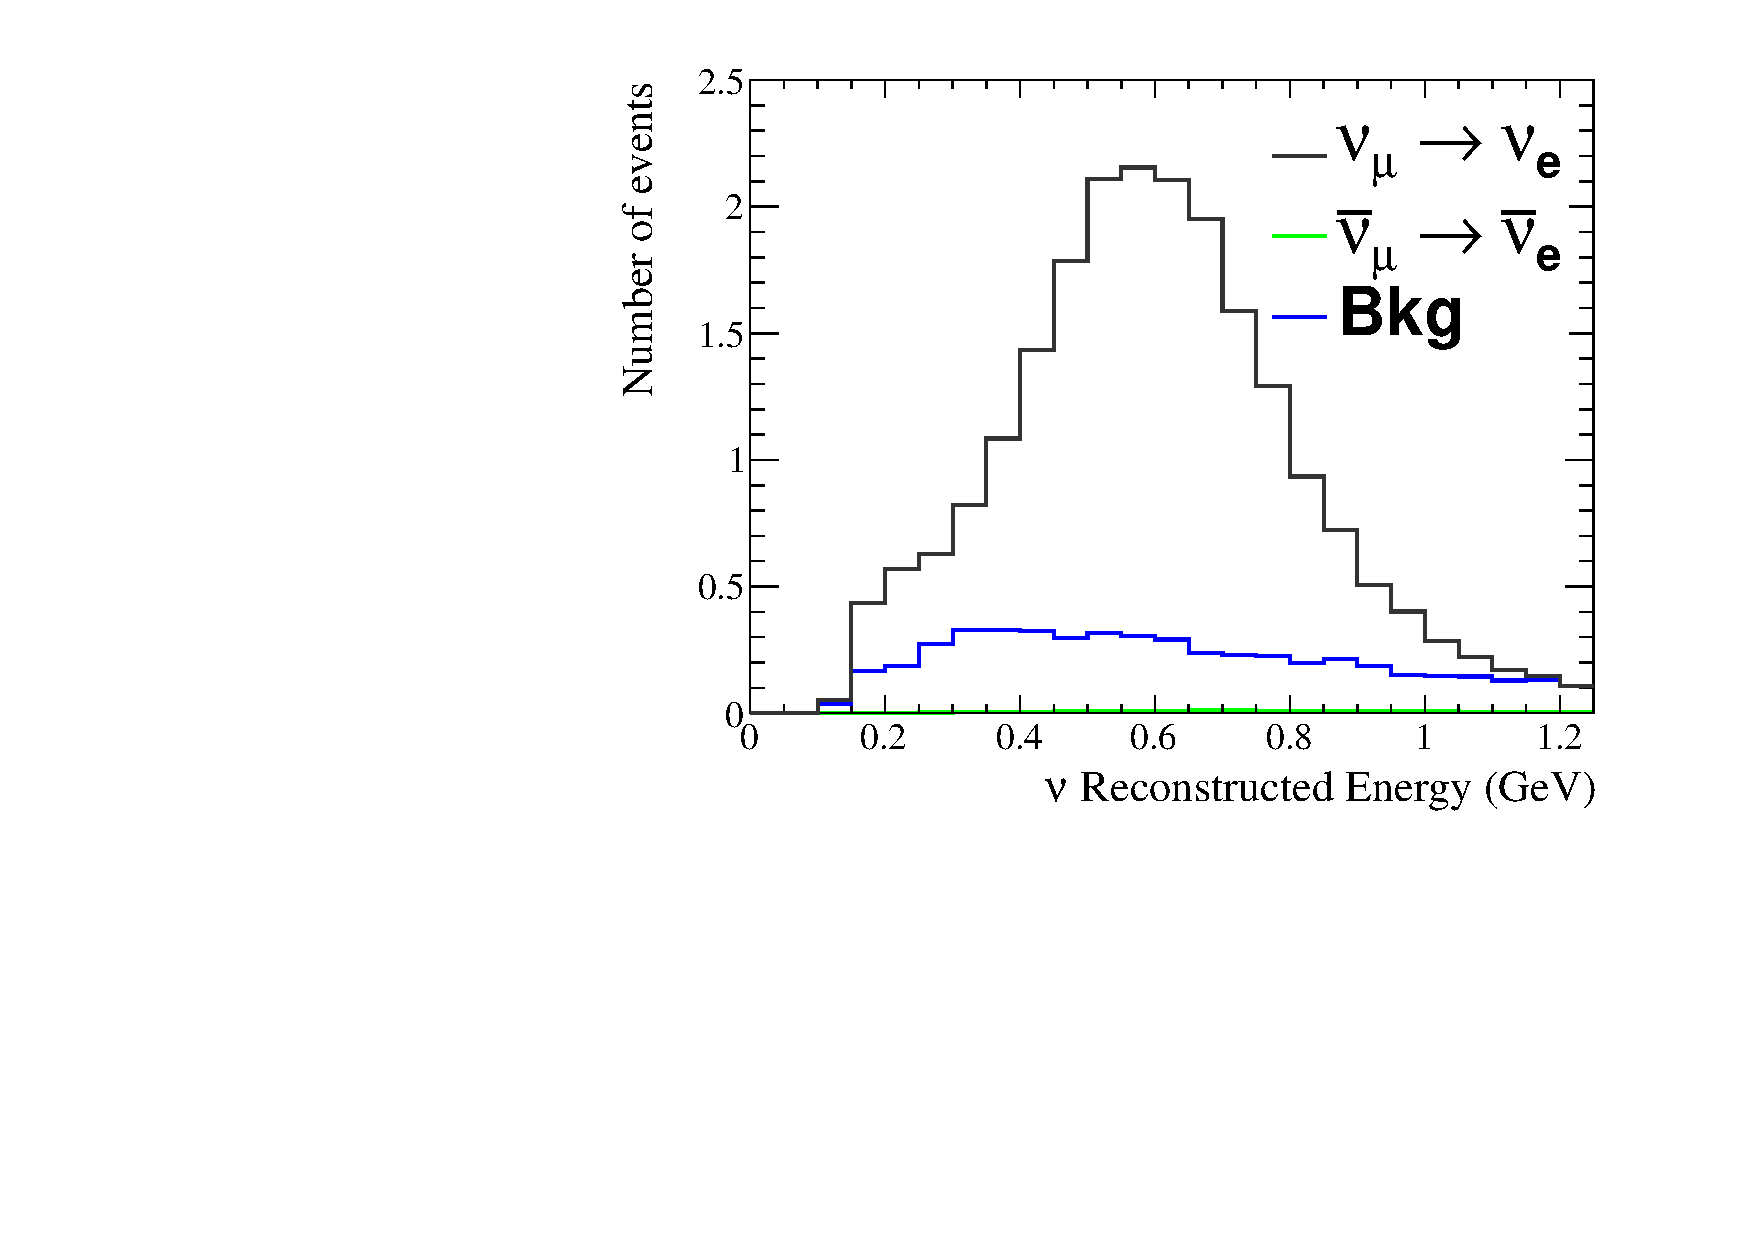
\includegraphics[width=18pc]{joint_plots/spectrum_predictions/template_ereco_1re_component.pdf}
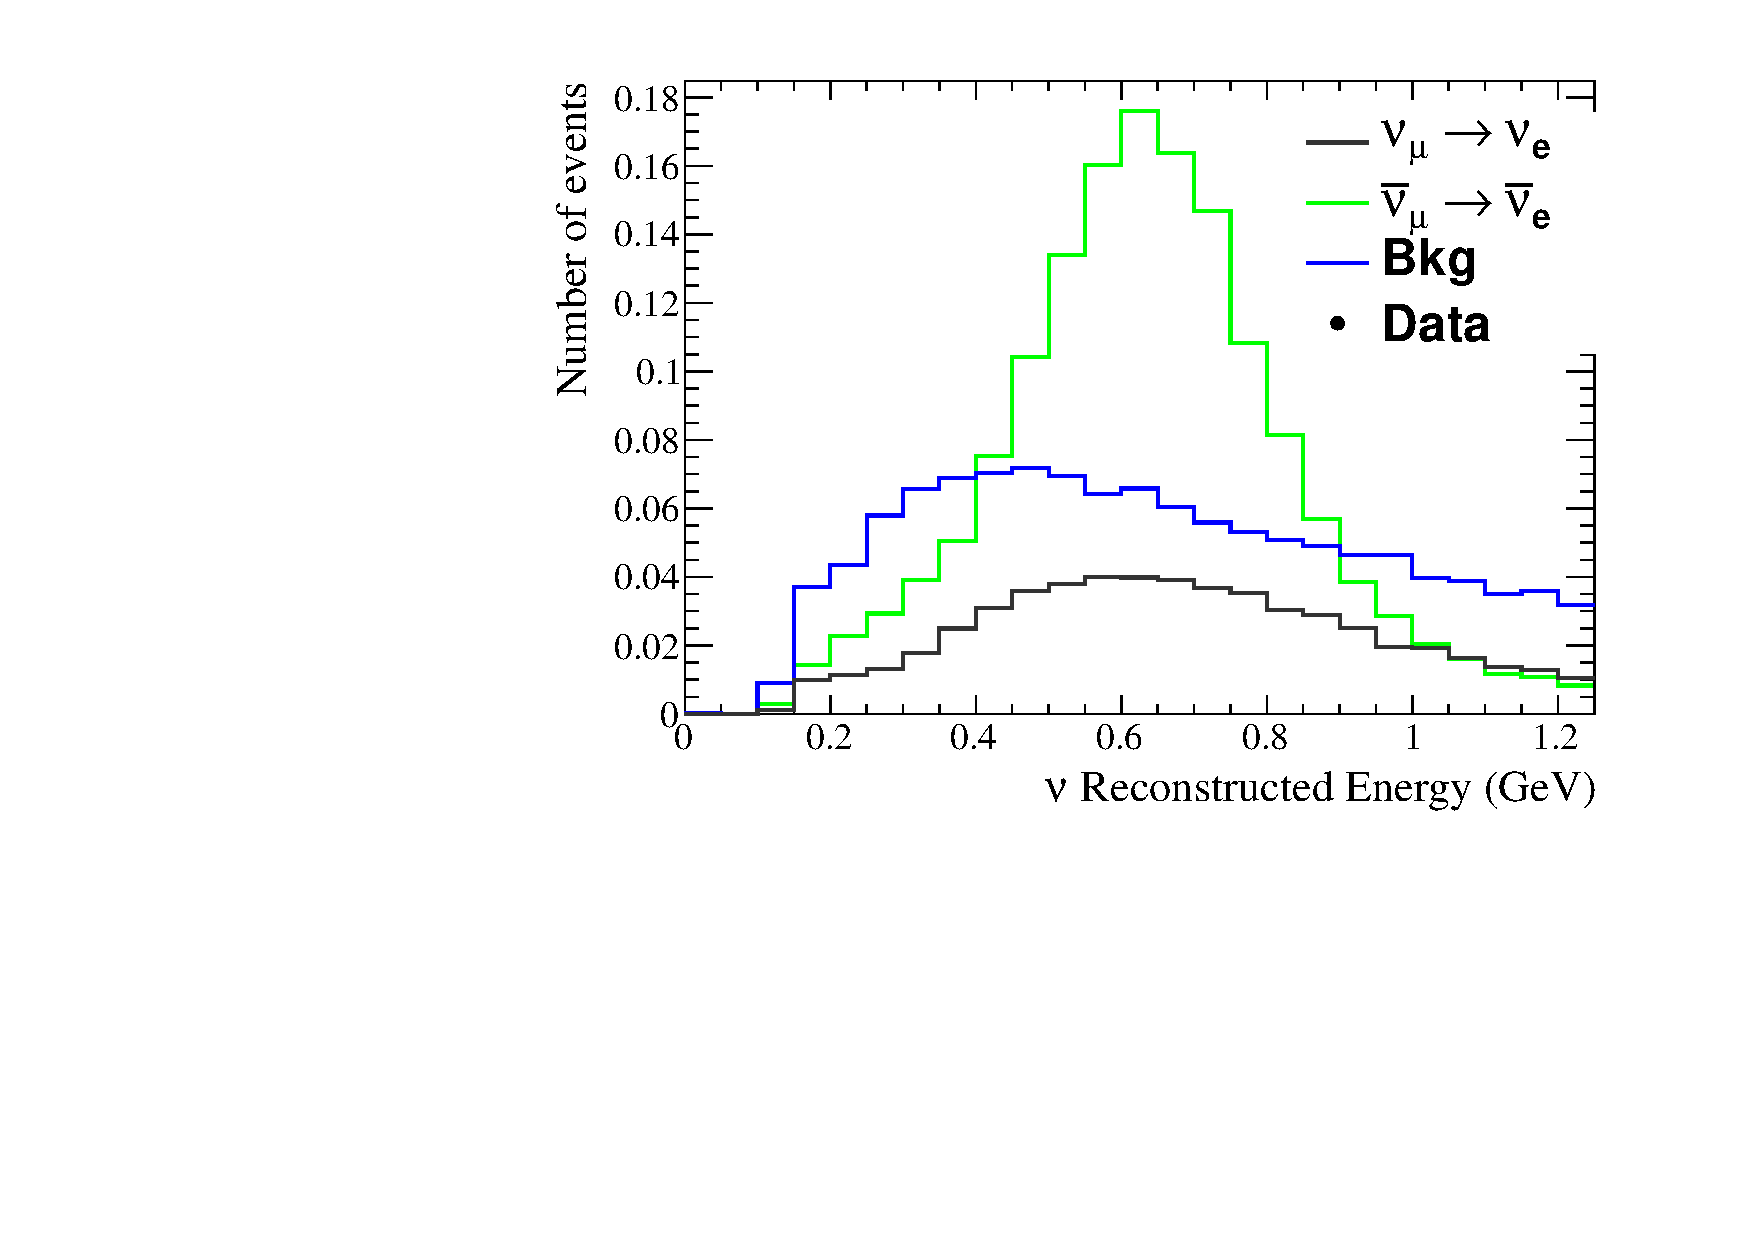
\includegraphics[width=18pc]{joint_plots/spectrum_predictions/template_ereco_rhc1re_component.pdf}
\caption {
  %  \huge{TO UPDATE} % caption is already ok
%{\large{ERECO SPECTRA WITH SEPARATED COMPONENTS}}
Predicted spectra of reconstructed neutrino energy 
for electron-like 
neutrino mode (left)
and
antineutrino mode (right)
events.
The distributions correspond to the collected statistics in the full Run 1-6 data set.
%for an exposure 
%of $6.914 \times 10^{20}$ POT in neutrino mode
%and
%of $4.011 \times 10^{20}$ POT in antineutrino mode.
The distributions are broken down by the following components:
$\bar{\nu}_{\mu} \to \bar{\nu}_e$ (green), 
$\nu_{\mu} \to \nu_e$ (black/white), 
background, 
which includes 
NC,
$\nu_e + \bar{\nu}_e$ intrinsic beam (yellow),
$\nu_{\mu}$ intrinsic beam (light blue)
and
$\bar{\nu}_{\mu}$ intrinsic beam (blue).
The spectra were generated with the systematic parameters measured with the ND280 data 
shown in \cref{tab:banff_uncertainties_flux_fhc},~\ref{tab:banff_uncertainties_flux_rhc},~\ref{tab:banff_uncertainties_xsec},
the nominal Super-K systematic parameters shown in \cref{tab:banff_uncertainties_skdetfsi}
and the oscillation parameters corresponding to the Asimov data set A shown in \cref{tab:osc_params_joint_asimov}.
It is not a stacked plot.
%The predicted spectrum of antineutrino mode 
%is scaled by a factor 7.
}
\label{fig:joint_ereco_components}
\end{figure*}


Another kinematical variable is thus needed in order to better separate different flavour / reaction compoonents.
In \cref{fig:joint_ereco_vs_theta_1re} and~\ref{fig:joint_ereco_vs_theta_rhc1re}
the 2-dimensional $E_{reco}$ vs $\theta$ spectra are shown for each flavour component and NC
for both neutrino and antineutrino mode $e$-like samples.
In particular the shapes of $\nu_{\mu} \rightarrow \nu_e$ and $\bar{\nu}_{\mu} \rightarrow \bar{\nu}_e$ 
distributions are quite different, thus this templates have a better capability to 
discriminate signal from background.
In general this template parametrization produces quite different shapes for all the main flavour and NC components.

\begin{figure*}[htb]
%\hspace{0.06\linewidth}
\center
\begin{subfigure}[b]{0.49\textwidth}
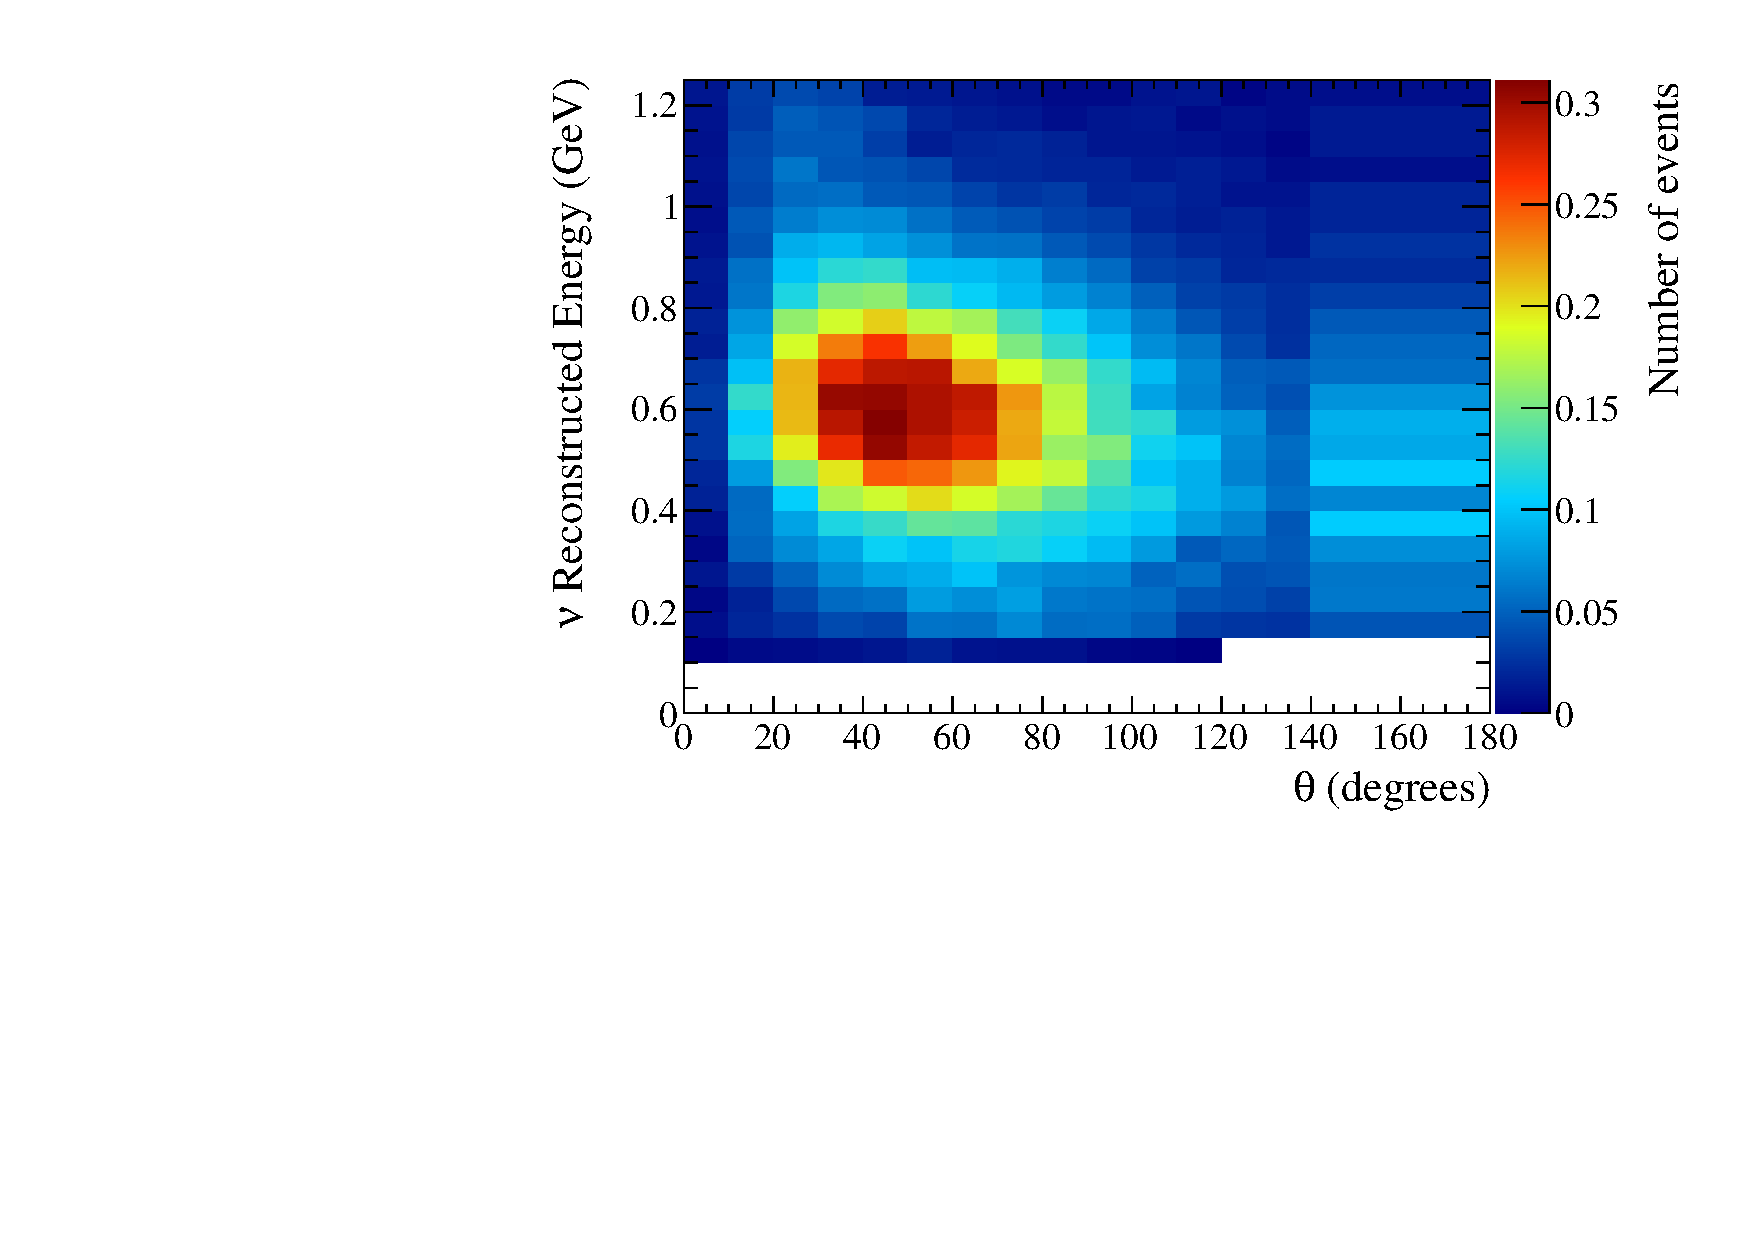
\includegraphics[width=0.9\textwidth]{joint_plots/spectrum_predictions/template_ereco_vs_theta_tot_1re.pdf}
\caption{Total}
\end{subfigure}\\
\begin{subfigure}[b]{0.49\textwidth}
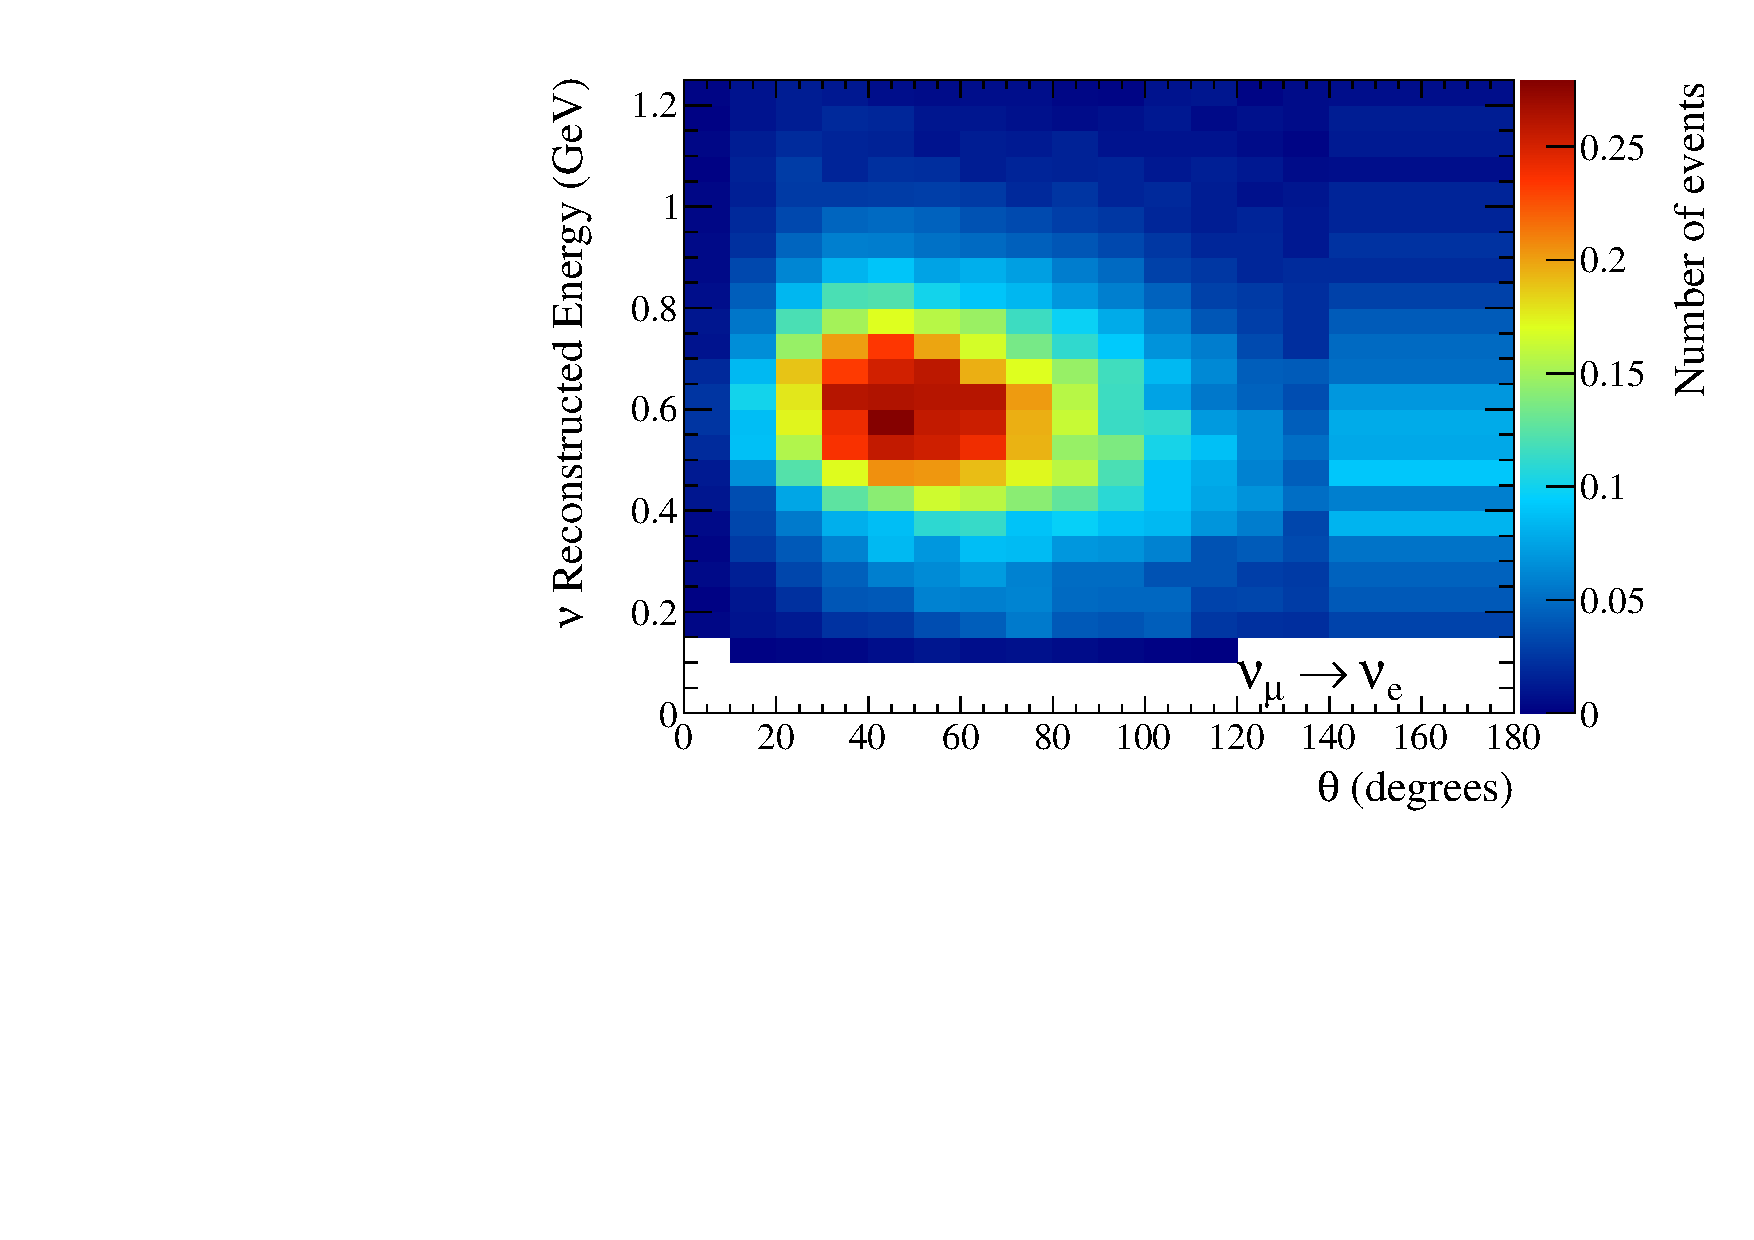
\includegraphics[width=0.9\textwidth]{joint_plots/spectrum_predictions/template_ereco_vs_theta_numutonue_1re.pdf}
\caption{$\nu_{\mu} \rightarrow \nu_e$.}
\end{subfigure}
\begin{subfigure}[b]{0.49\textwidth}
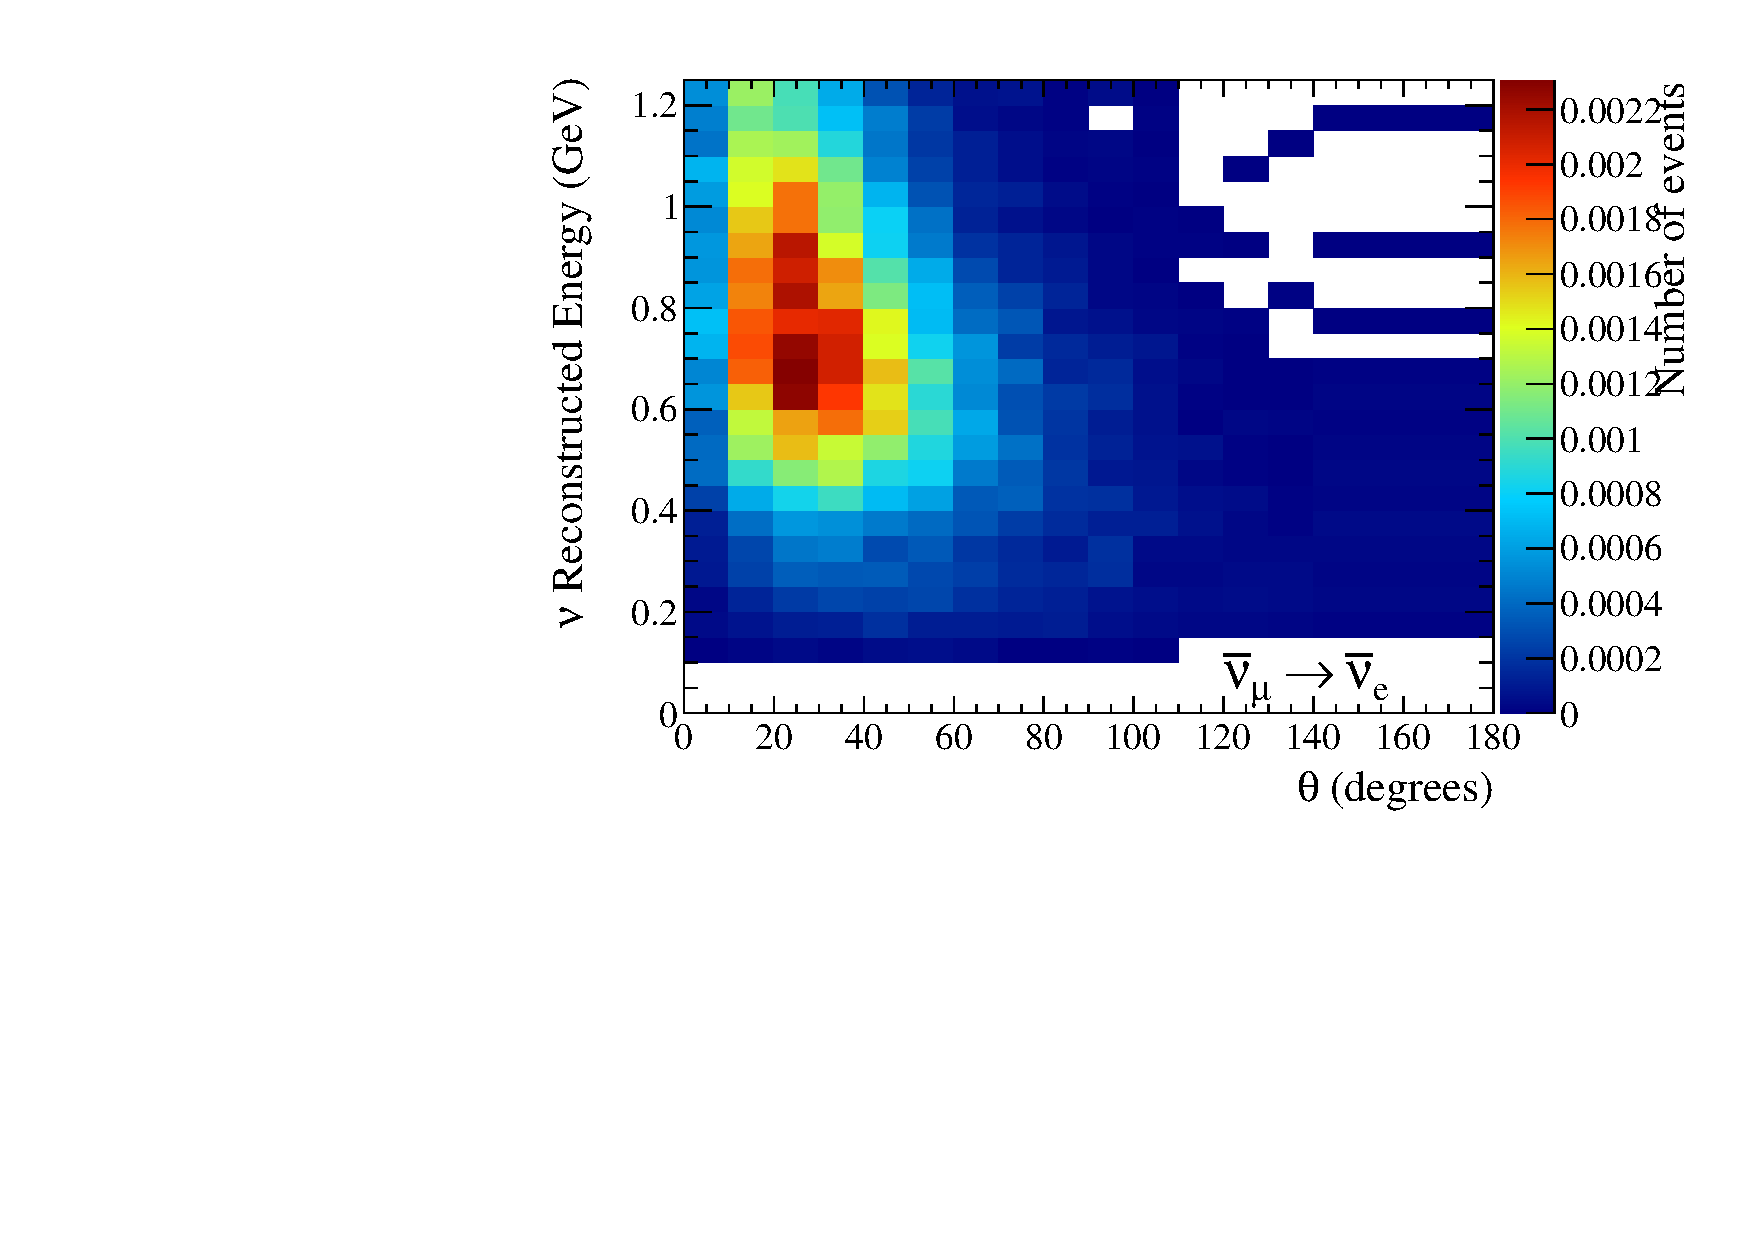
\includegraphics[width=0.9\textwidth]{joint_plots/spectrum_predictions/template_ereco_vs_theta_numubartonuebar_1re.pdf}
\caption{$\bar{\nu}_{\mu} \rightarrow \bar{\nu}_e$.}
\end{subfigure}
\begin{subfigure}[b]{0.49\textwidth}
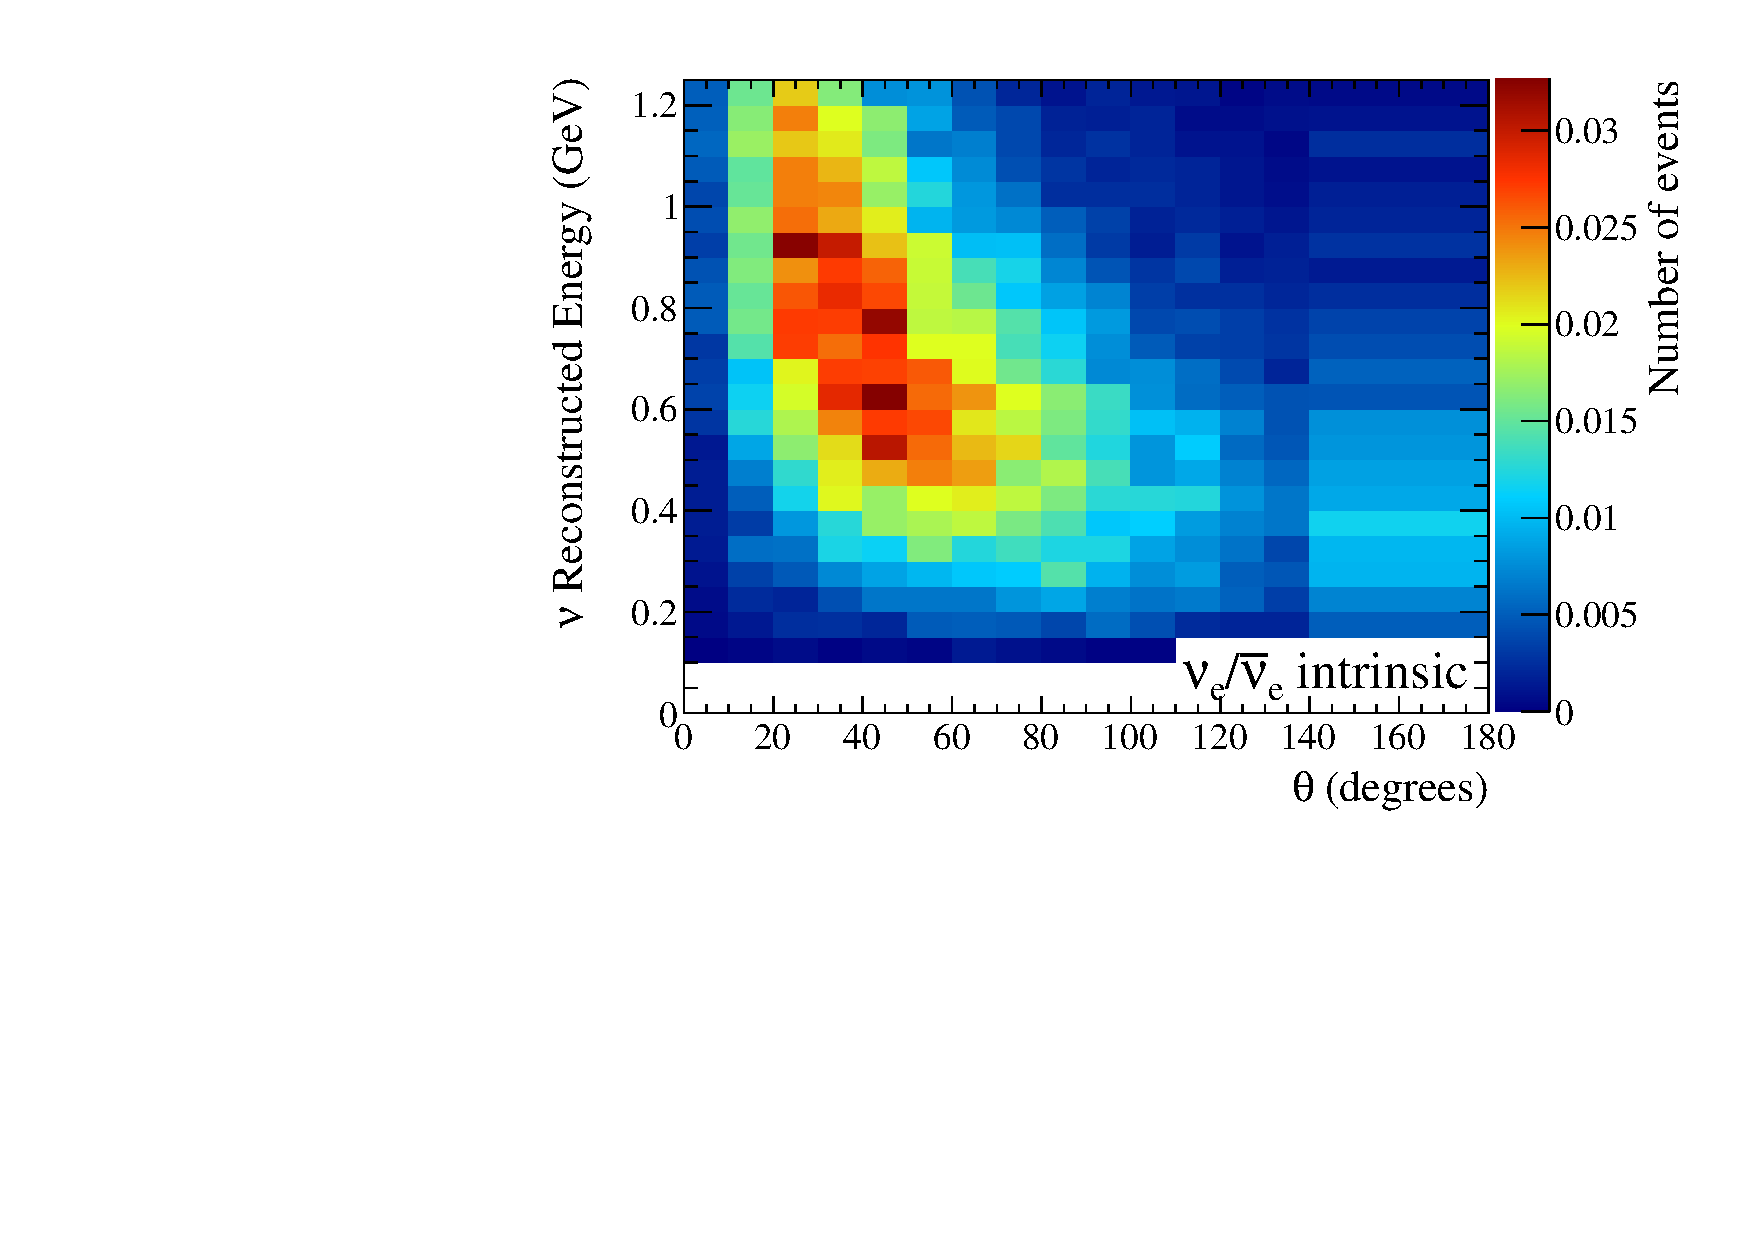
\includegraphics[width=0.9\textwidth]{joint_plots/spectrum_predictions/template_ereco_vs_theta_nuebeam_1re.pdf}
\caption{$\nu_{e}$ + $\bar{\nu}_e$ intrinsic beam.}
\end{subfigure}
\begin{subfigure}[b]{0.49\textwidth}
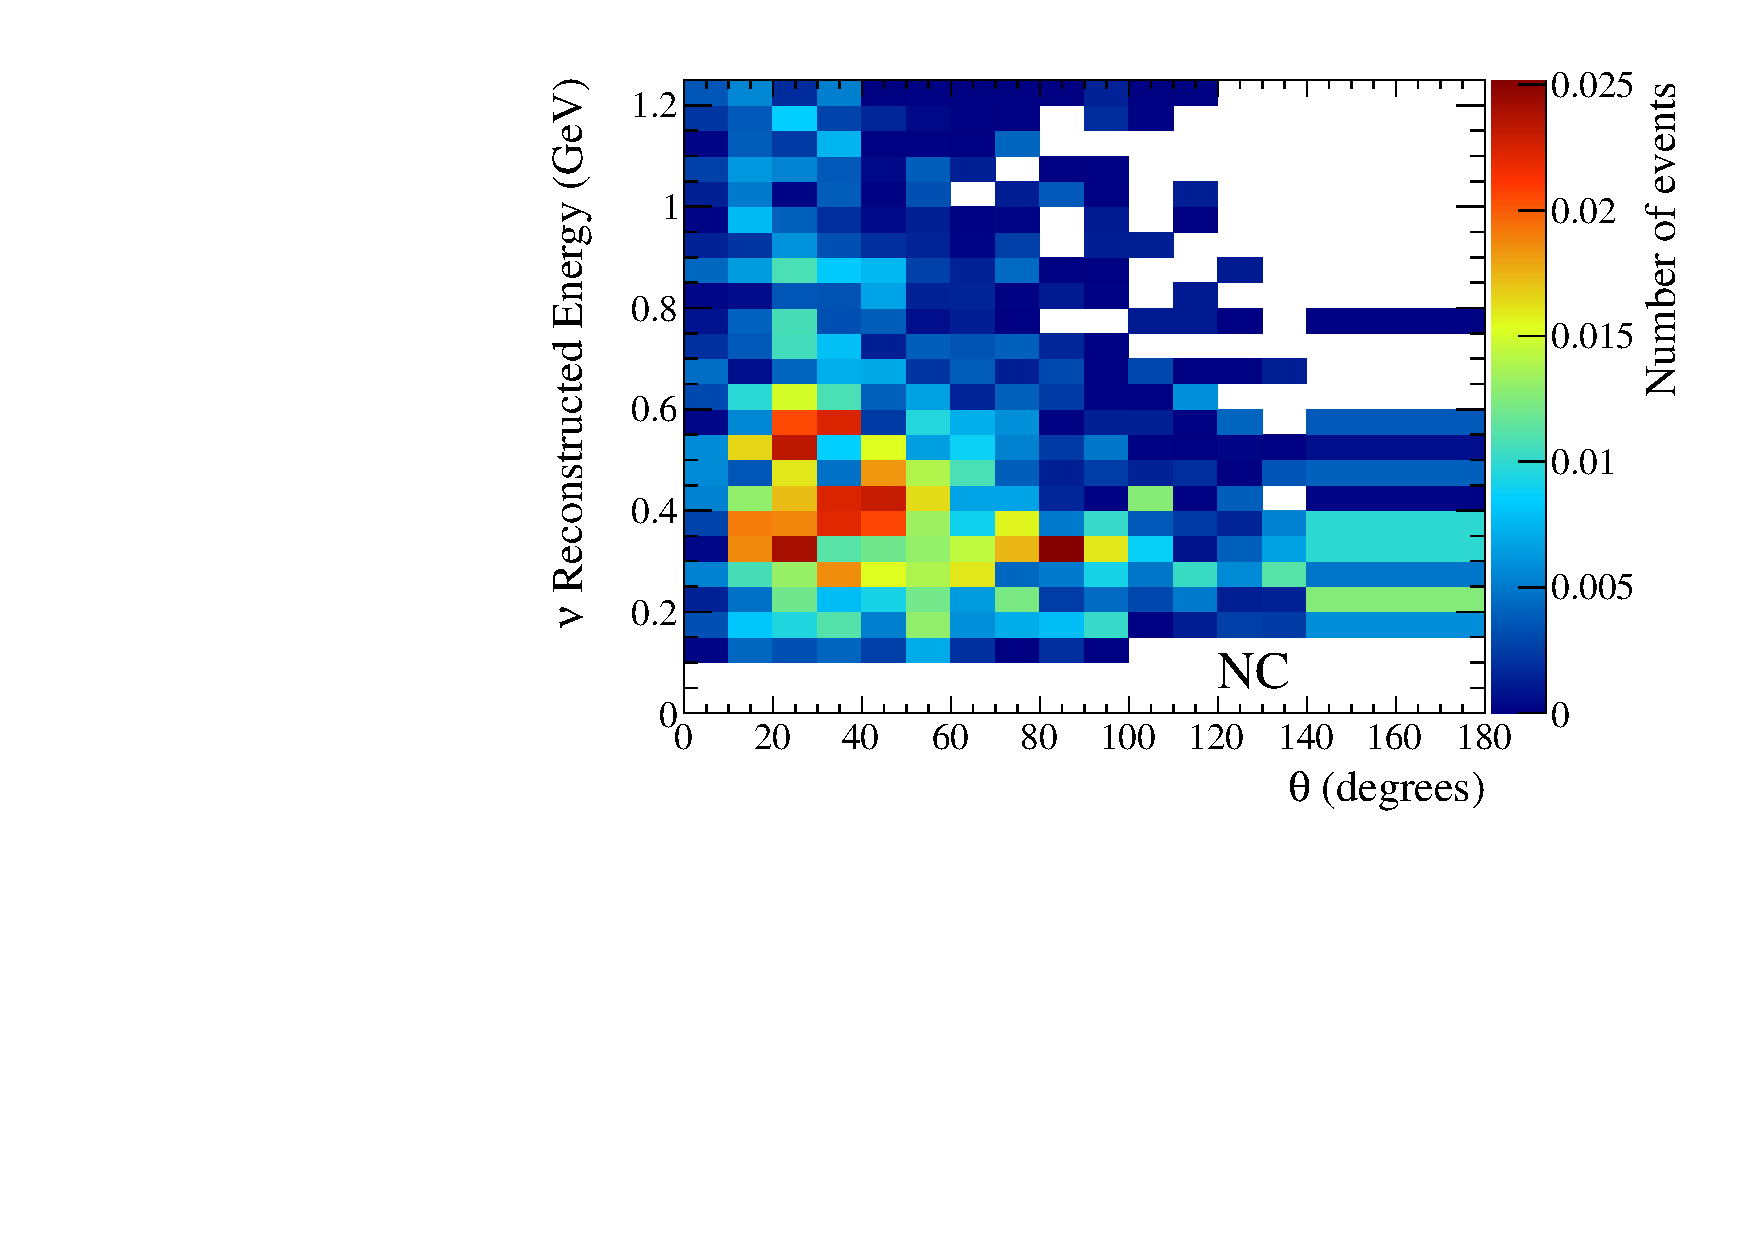
\includegraphics[width=0.9\textwidth]{joint_plots/spectrum_predictions/template_ereco_vs_theta_nc_1re.pdf}
\caption{Neutral current.}
\end{subfigure}
\begin{subfigure}[b]{0.49\textwidth}
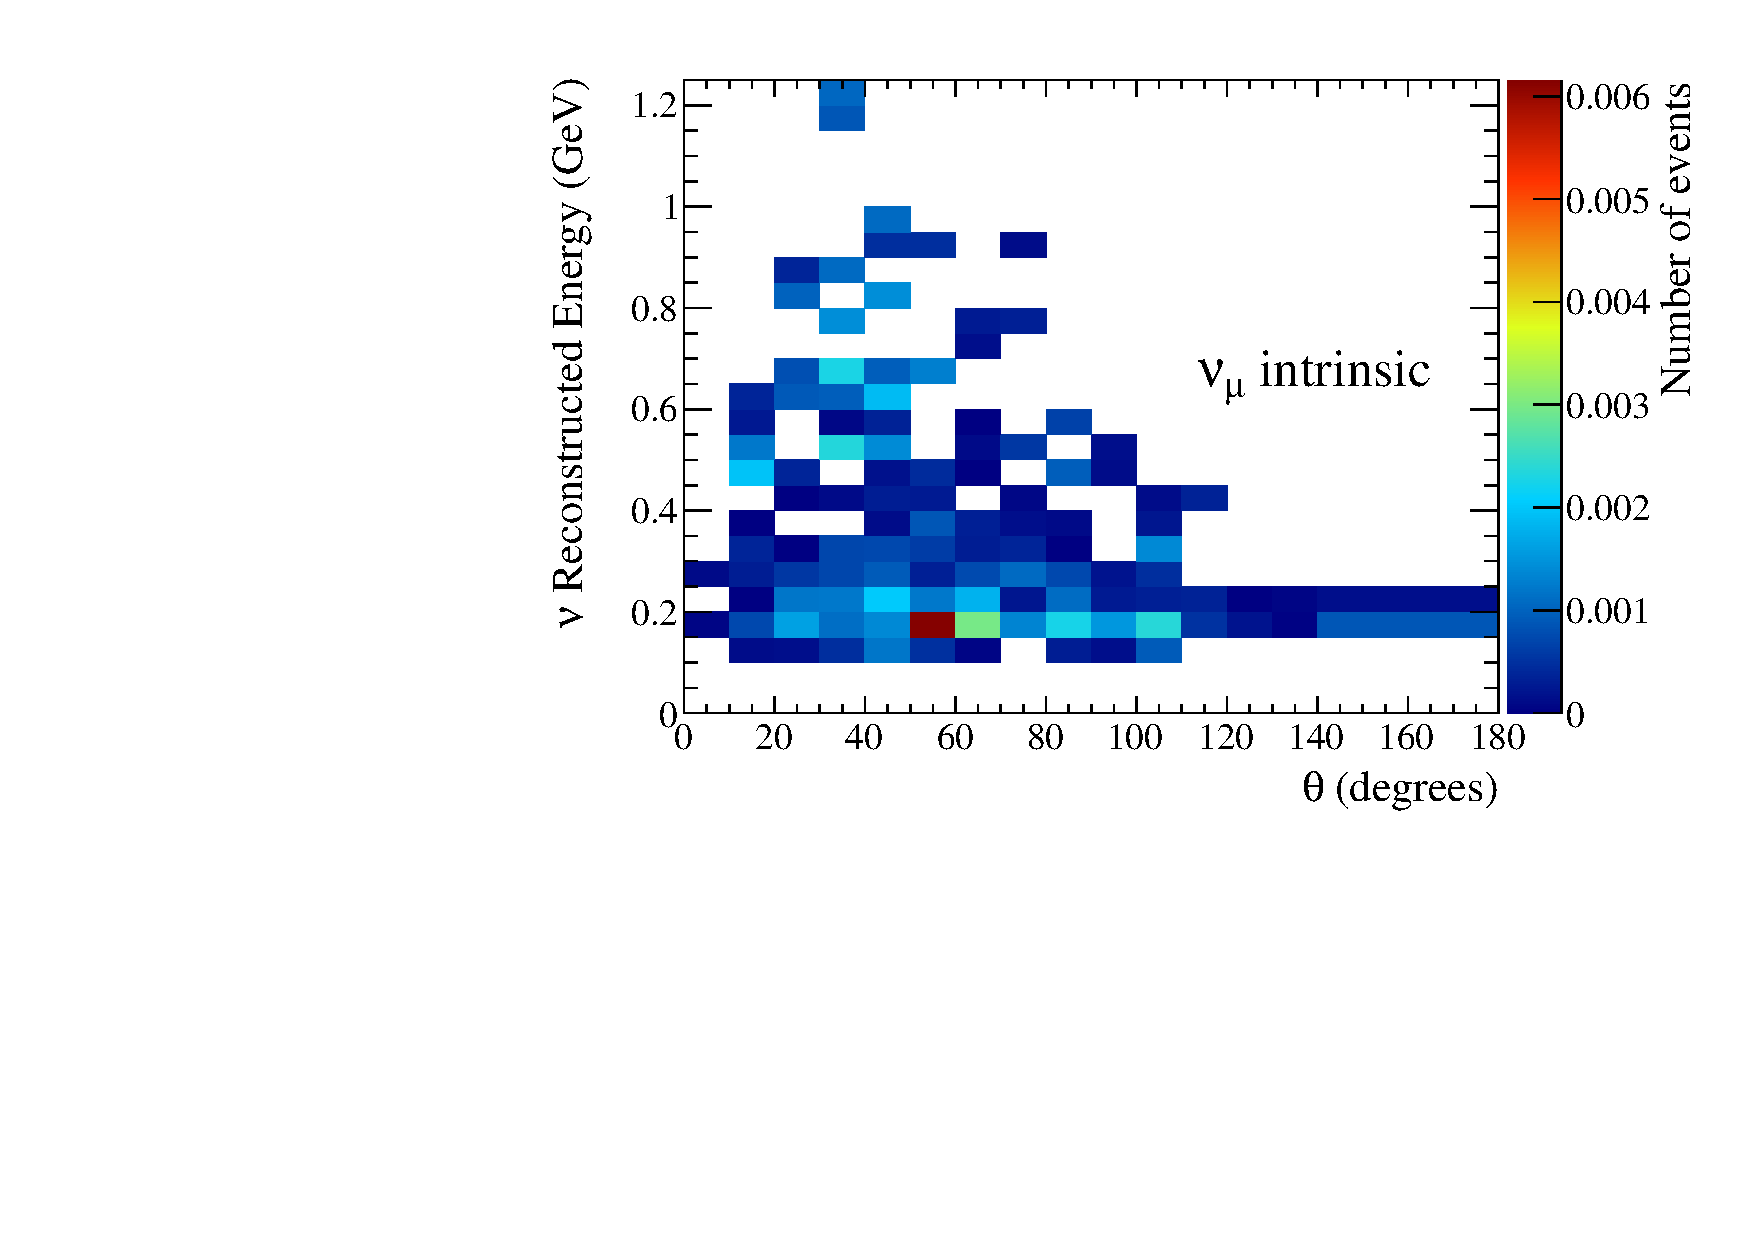
\includegraphics[width=0.9\textwidth]{joint_plots/spectrum_predictions/template_ereco_vs_theta_numubeam_1re.pdf}
\caption{$\nu_{\mu}$ intrinsic beam.}
\end{subfigure}
\begin{subfigure}[b]{0.49\textwidth}
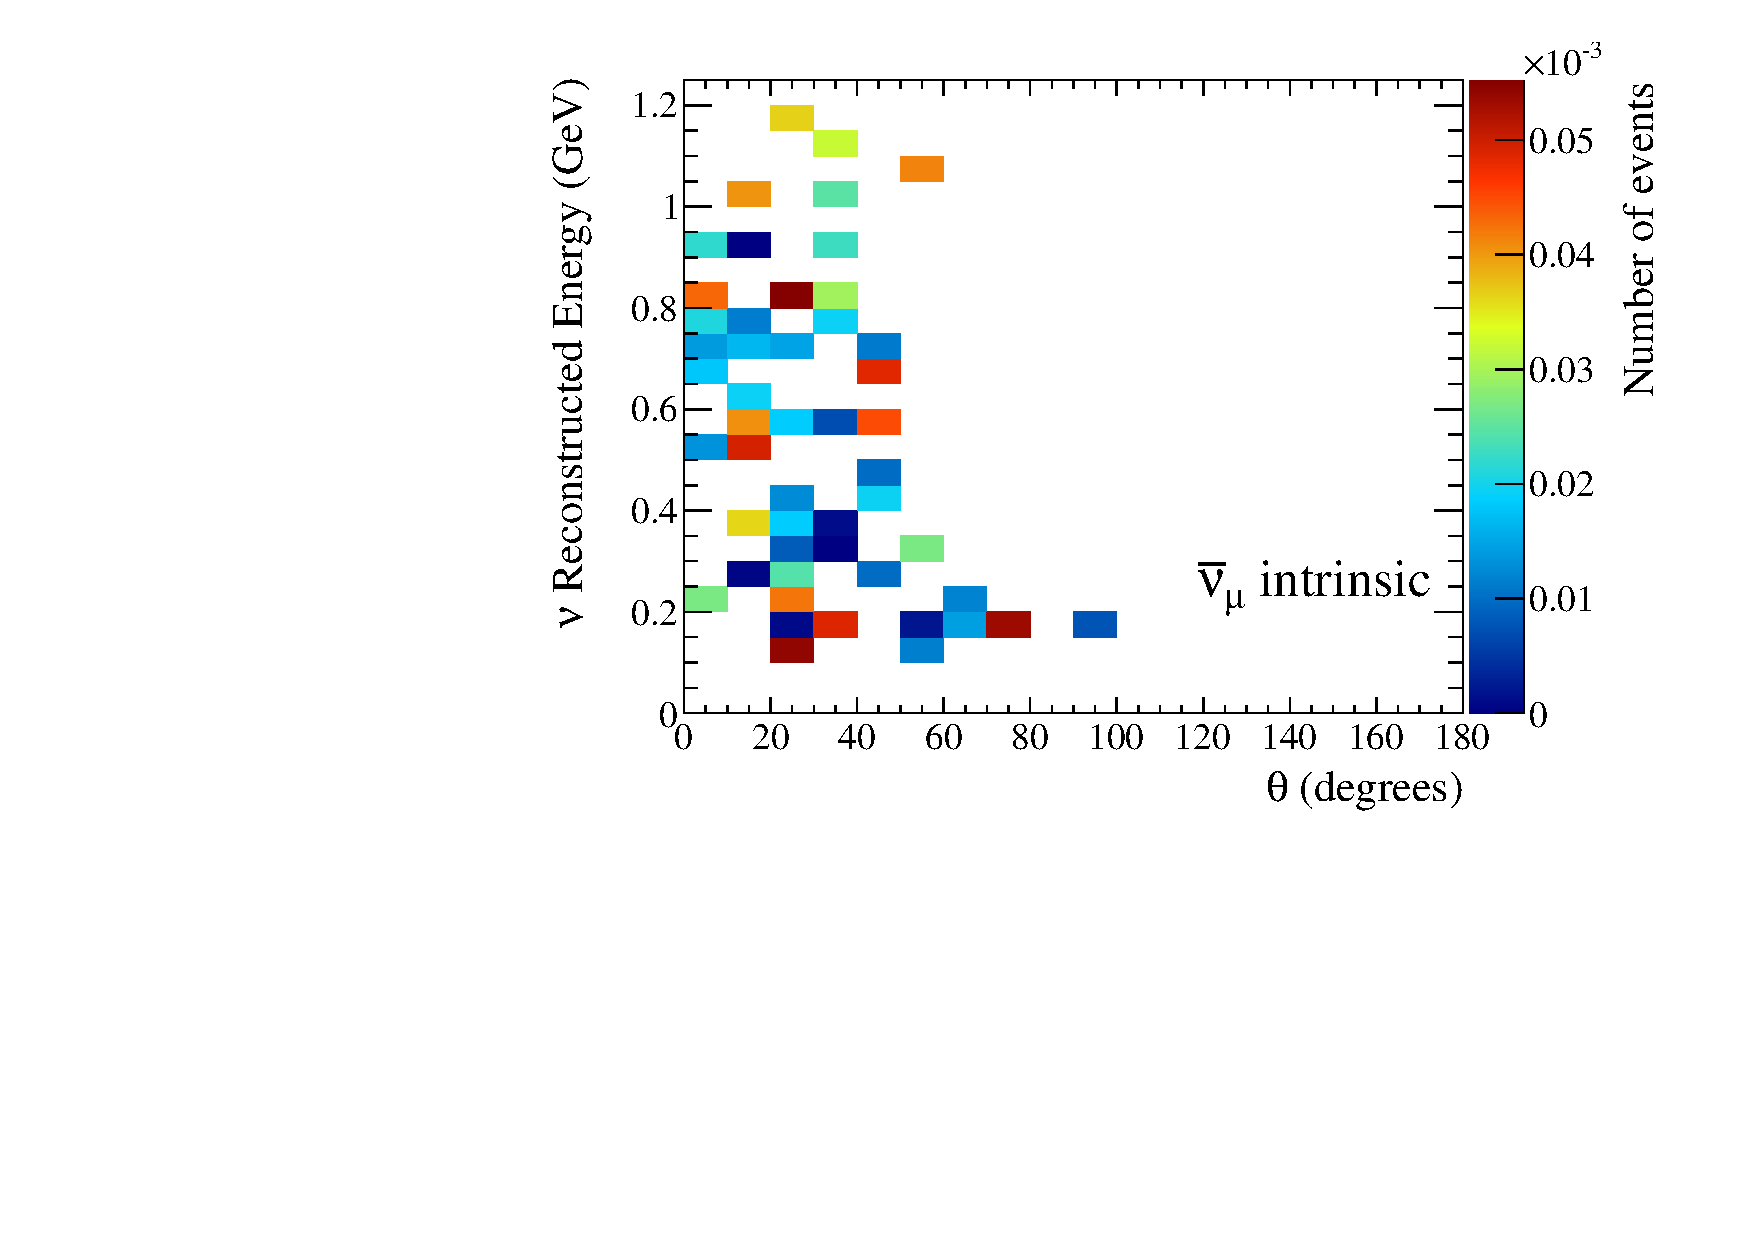
\includegraphics[width=0.9\textwidth]{joint_plots/spectrum_predictions/template_ereco_vs_theta_numubarbeam_1re.pdf}
\caption{$\bar{\nu}_{\mu}$ intrinsic beam.}
\end{subfigure}
\caption {
Predicted spectra of electron-like events
as a function of the reconstructed neutrino energy and
the angle between the outgoing lepton and the neutrino direction.
The distributions correspond to the collected statistics in the full Run 1-6 data set.
%for an exposure 
%of $6.914 \times 10^{20}$ POT in neutrino mode.
%and
%of $4.011 \times 10^{20}$ POT in antineutrino mode.
From top left to bottom right the following components are shown:
total,
$\nu_{\mu} \rightarrow \nu_e$,
$\bar{\nu}_{\mu} \rightarrow \bar{\nu}_e$,
$\nu_e + \bar{\nu}_e$ intrinsic beam,
NC,
$\nu_{\mu}$ intrinsic beam
and
$\bar{\nu}_{\mu}$ intrinsic beam.
The spectra were generated with the systematic parameters measured with the ND280 data 
shown in \cref{tab:banff_uncertainties_flux_fhc},~\ref{tab:banff_uncertainties_flux_rhc},~\ref{tab:banff_uncertainties_xsec},
the nominal Super-K systematic parameters shown in \cref{tab:banff_uncertainties_skdetfsi}
and the oscillation parameters corresponding to the Asimov data set A shown in \cref{tab:osc_params_joint_asimov}.
}
\label{fig:joint_ereco_vs_theta_1re}
\end{figure*}

\begin{figure*}[htb]
%\hspace{0.06\linewidth}
\center
\begin{subfigure}[b]{0.49\textwidth}
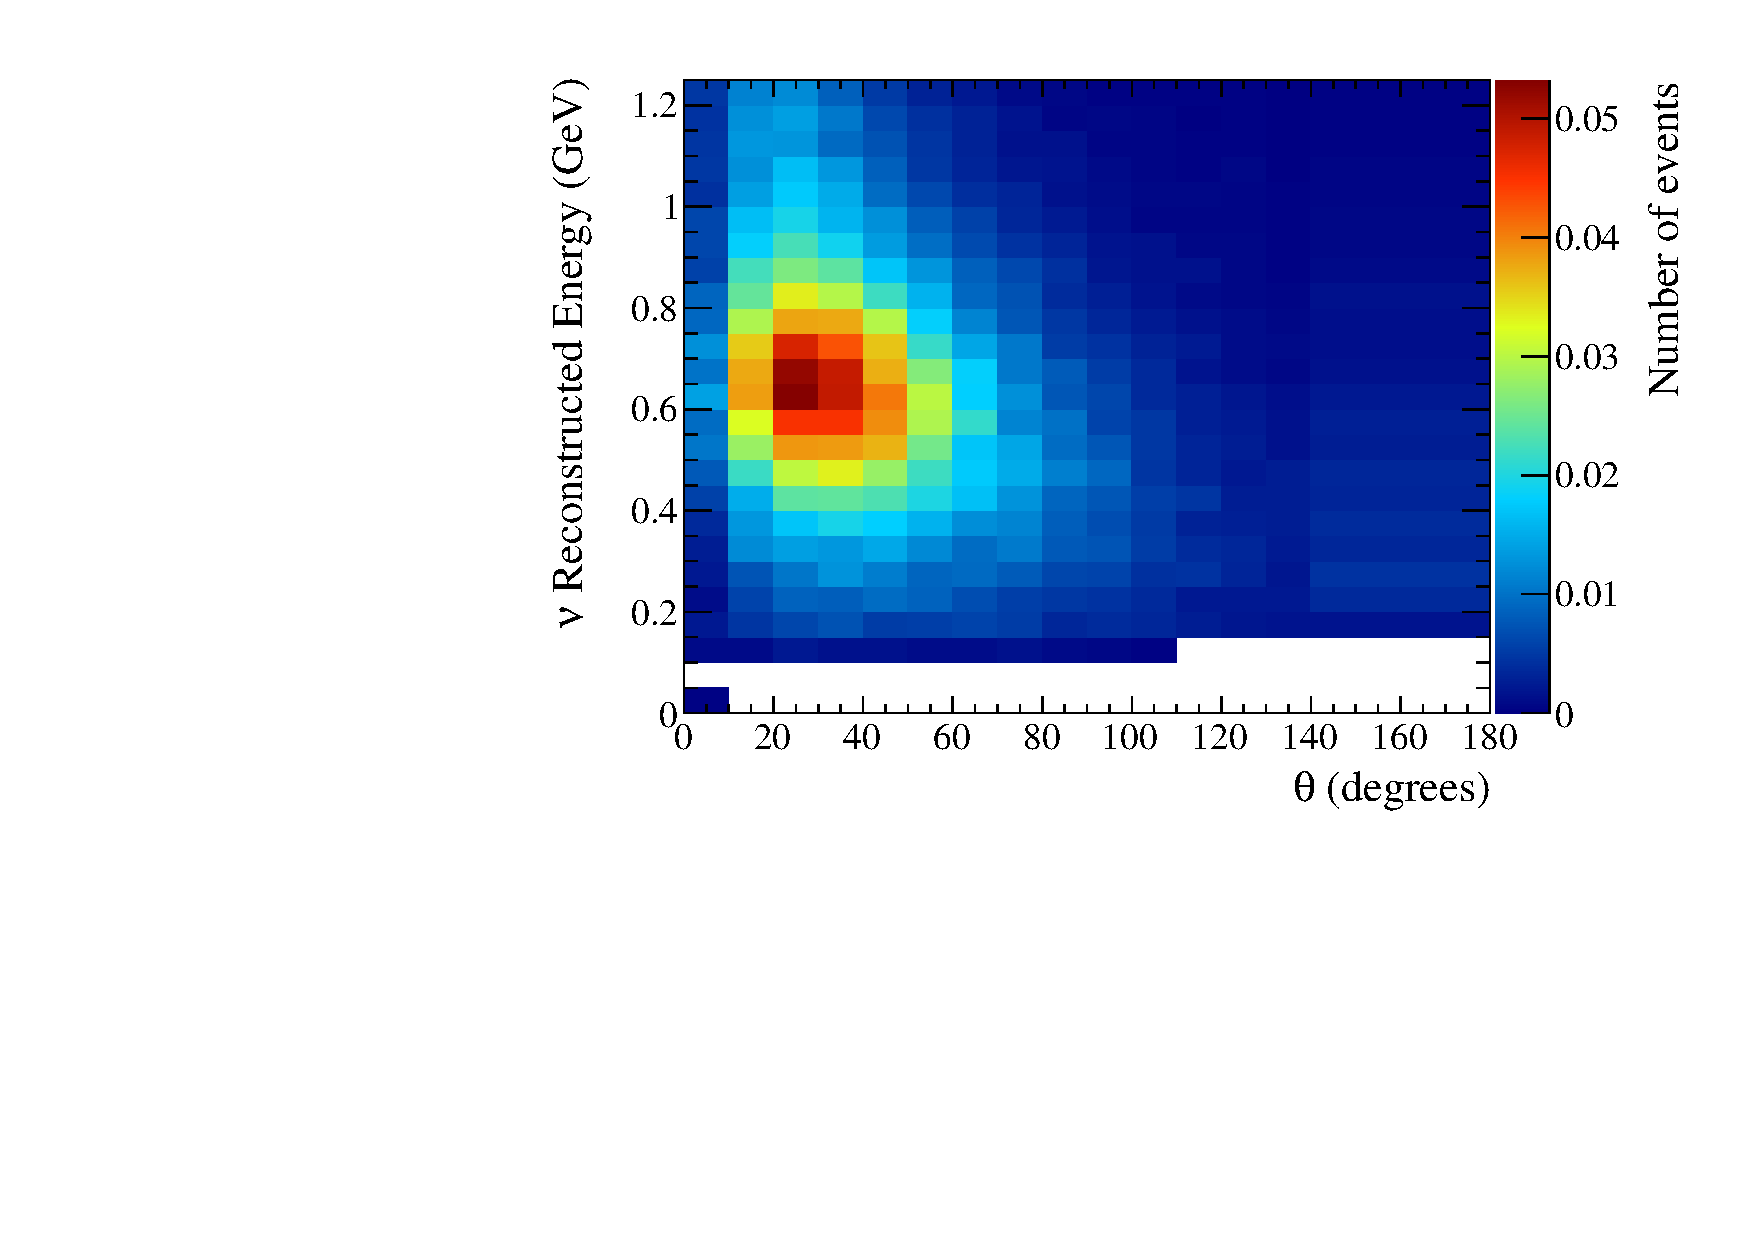
\includegraphics[width=0.9\textwidth]{joint_plots/spectrum_predictions/template_ereco_vs_theta_tot_rhc1re.pdf}\\
\caption{Total}
\end{subfigure}\\
\begin{subfigure}[b]{0.49\textwidth}
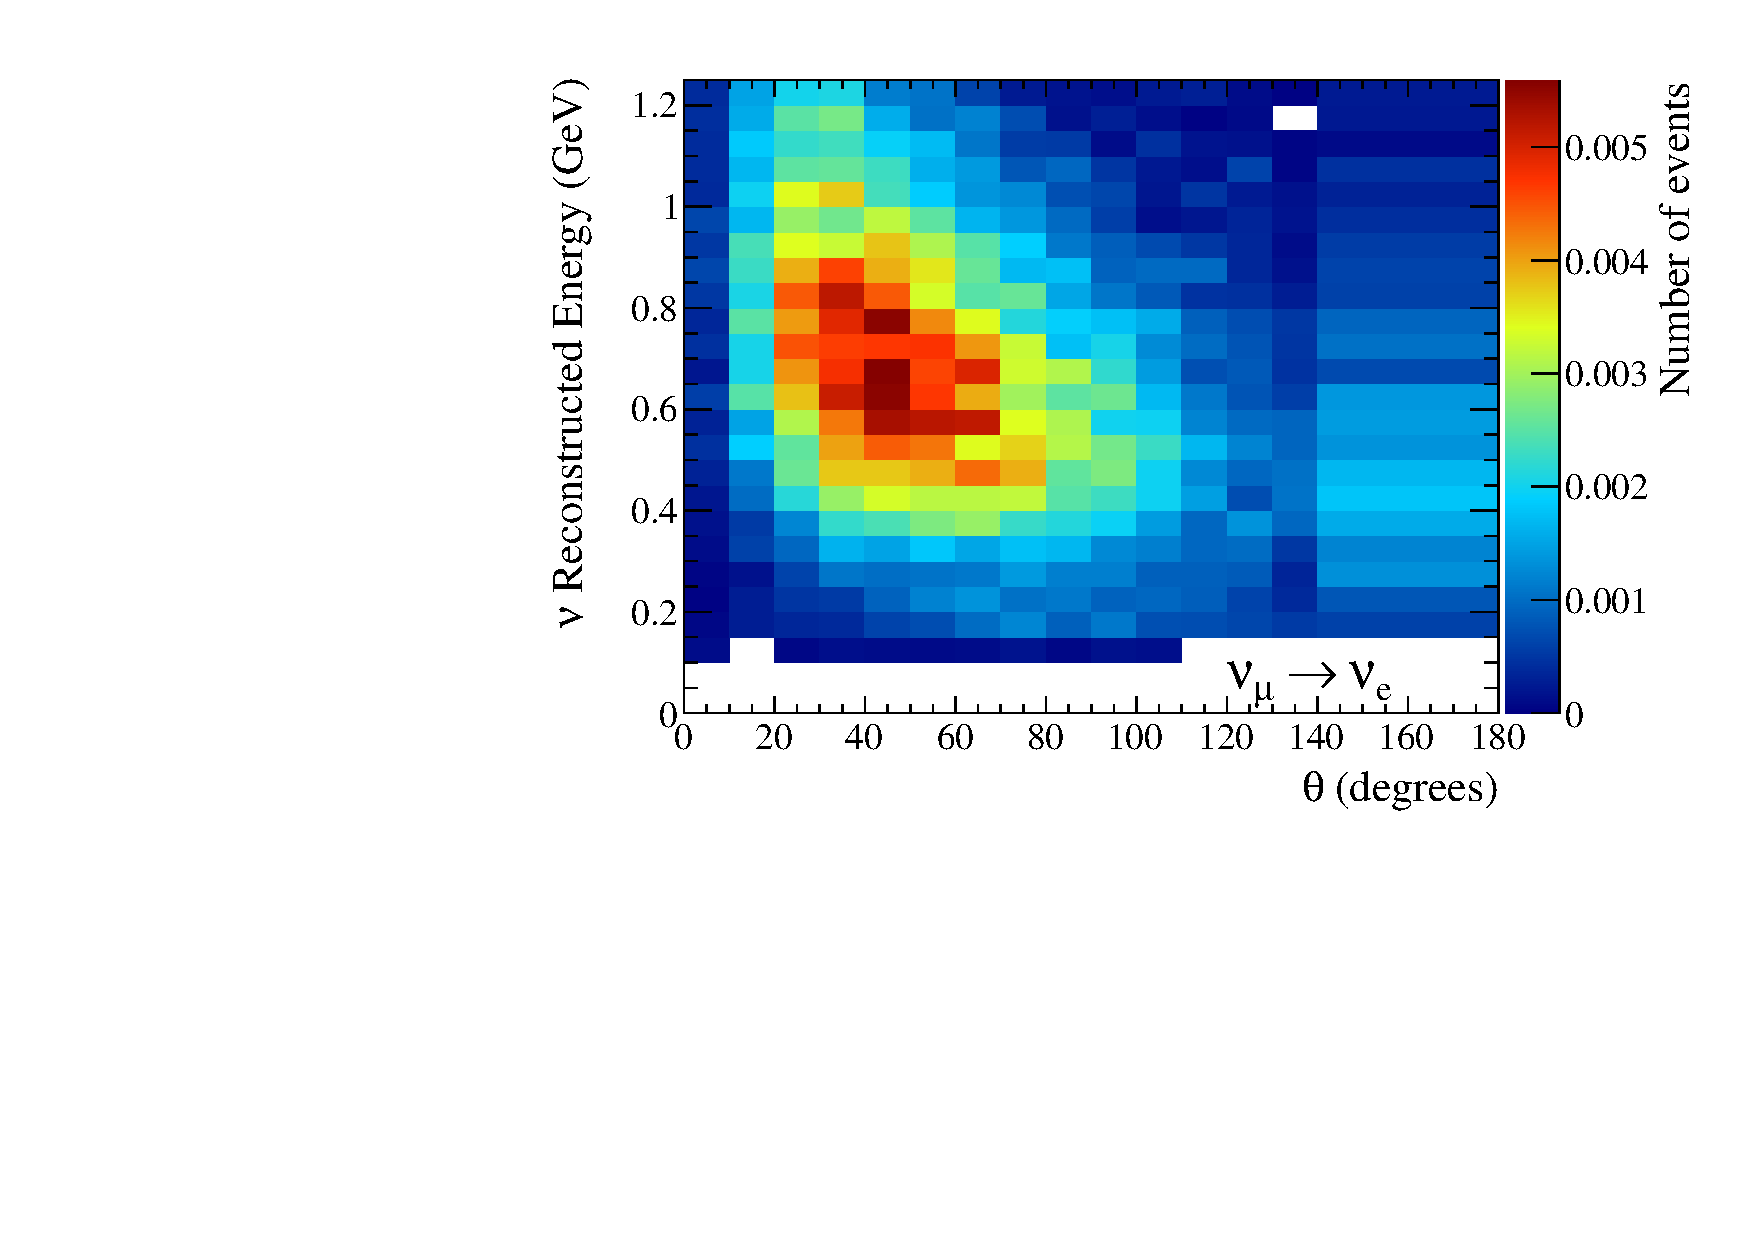
\includegraphics[width=0.9\textwidth]{joint_plots/spectrum_predictions/template_ereco_vs_theta_numutonue_rhc1re.pdf}
\caption{$\nu_{\mu} \rightarrow \nu_e$.}
\end{subfigure}
\begin{subfigure}[b]{0.49\textwidth}
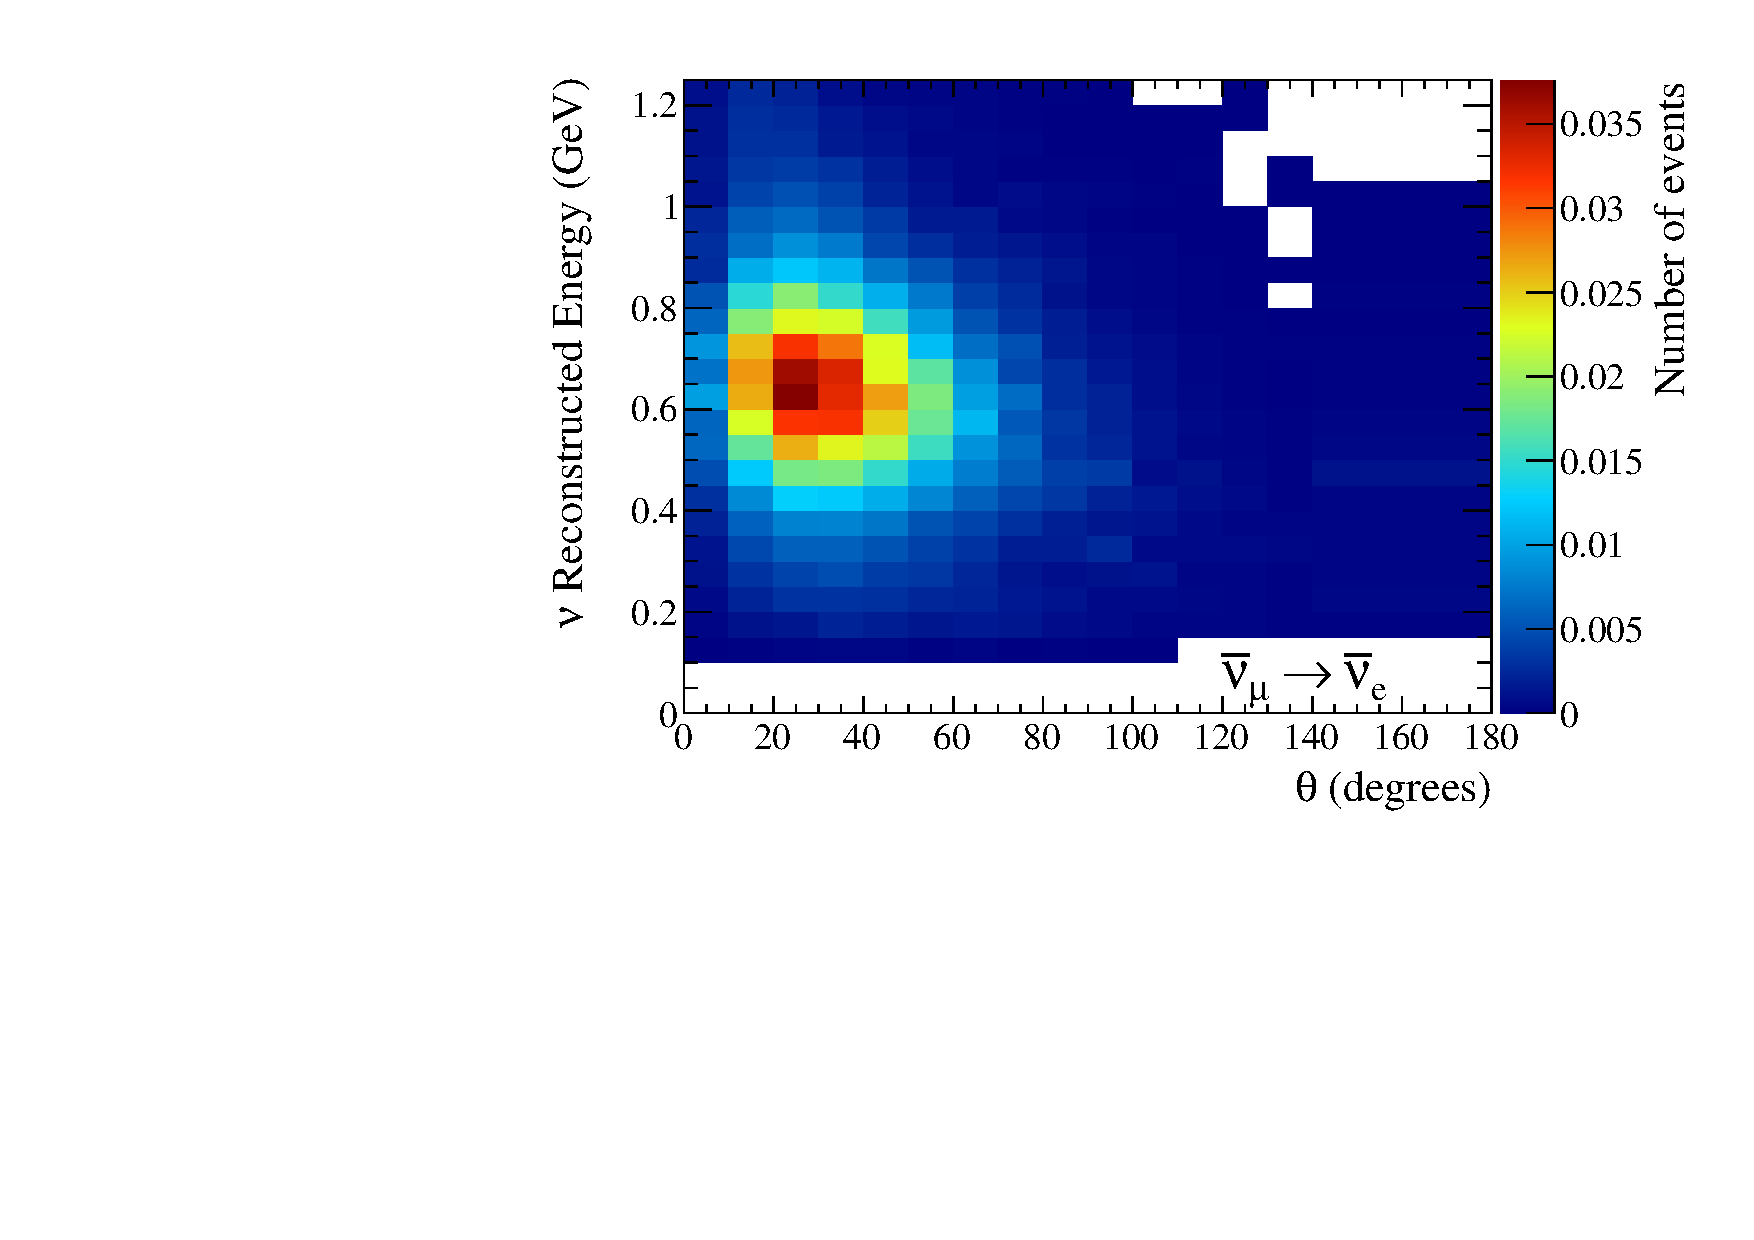
\includegraphics[width=0.9\textwidth]{joint_plots/spectrum_predictions/template_ereco_vs_theta_numubartonuebar_rhc1re.pdf}
\caption{$\bar{\nu}_{\mu} \rightarrow \bar{\nu}_e$.}
\end{subfigure}
\begin{subfigure}[b]{0.49\textwidth}
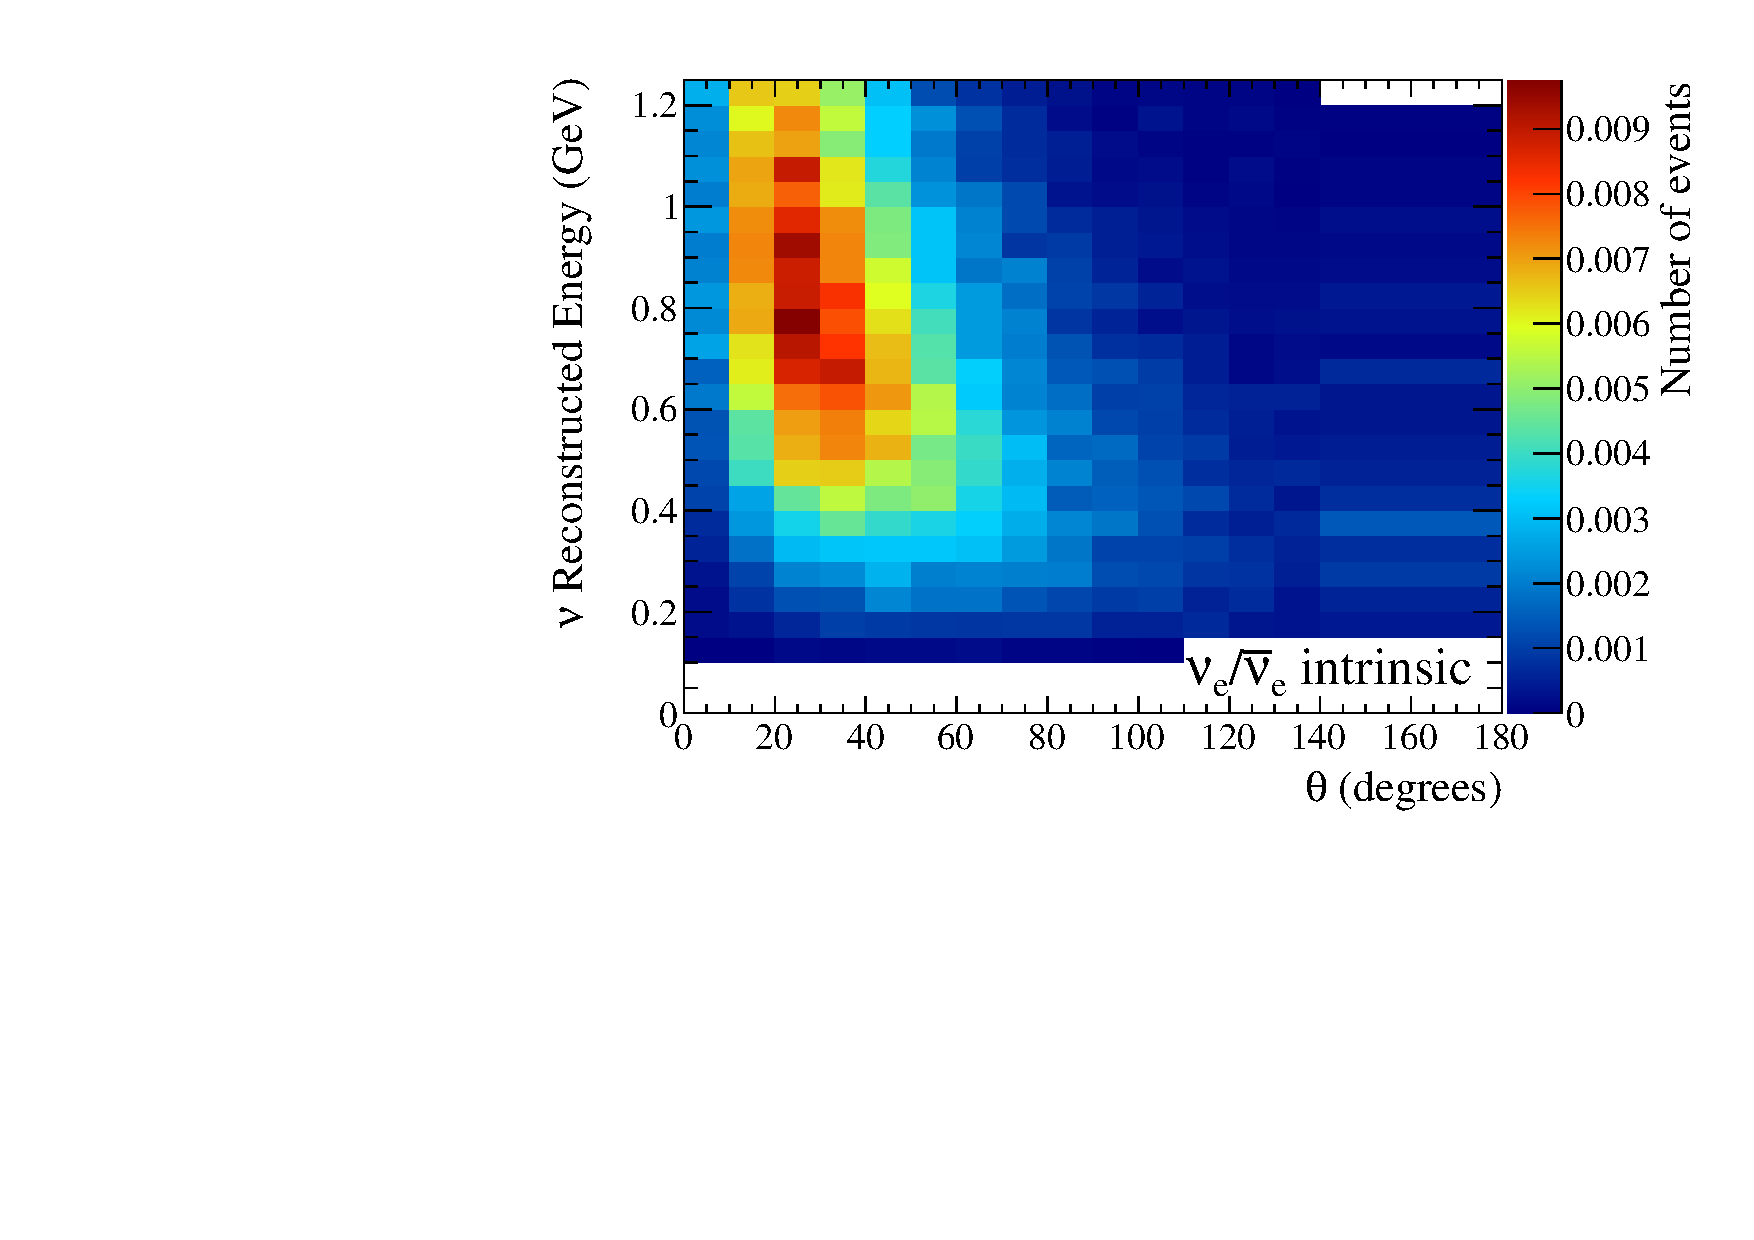
\includegraphics[width=0.9\textwidth]{joint_plots/spectrum_predictions/template_ereco_vs_theta_nuebeam_rhc1re.pdf}
\caption{$\nu_{e}$ + $\bar{\nu}_e$ intrinsic beam.}
\end{subfigure}
\begin{subfigure}[b]{0.49\textwidth}
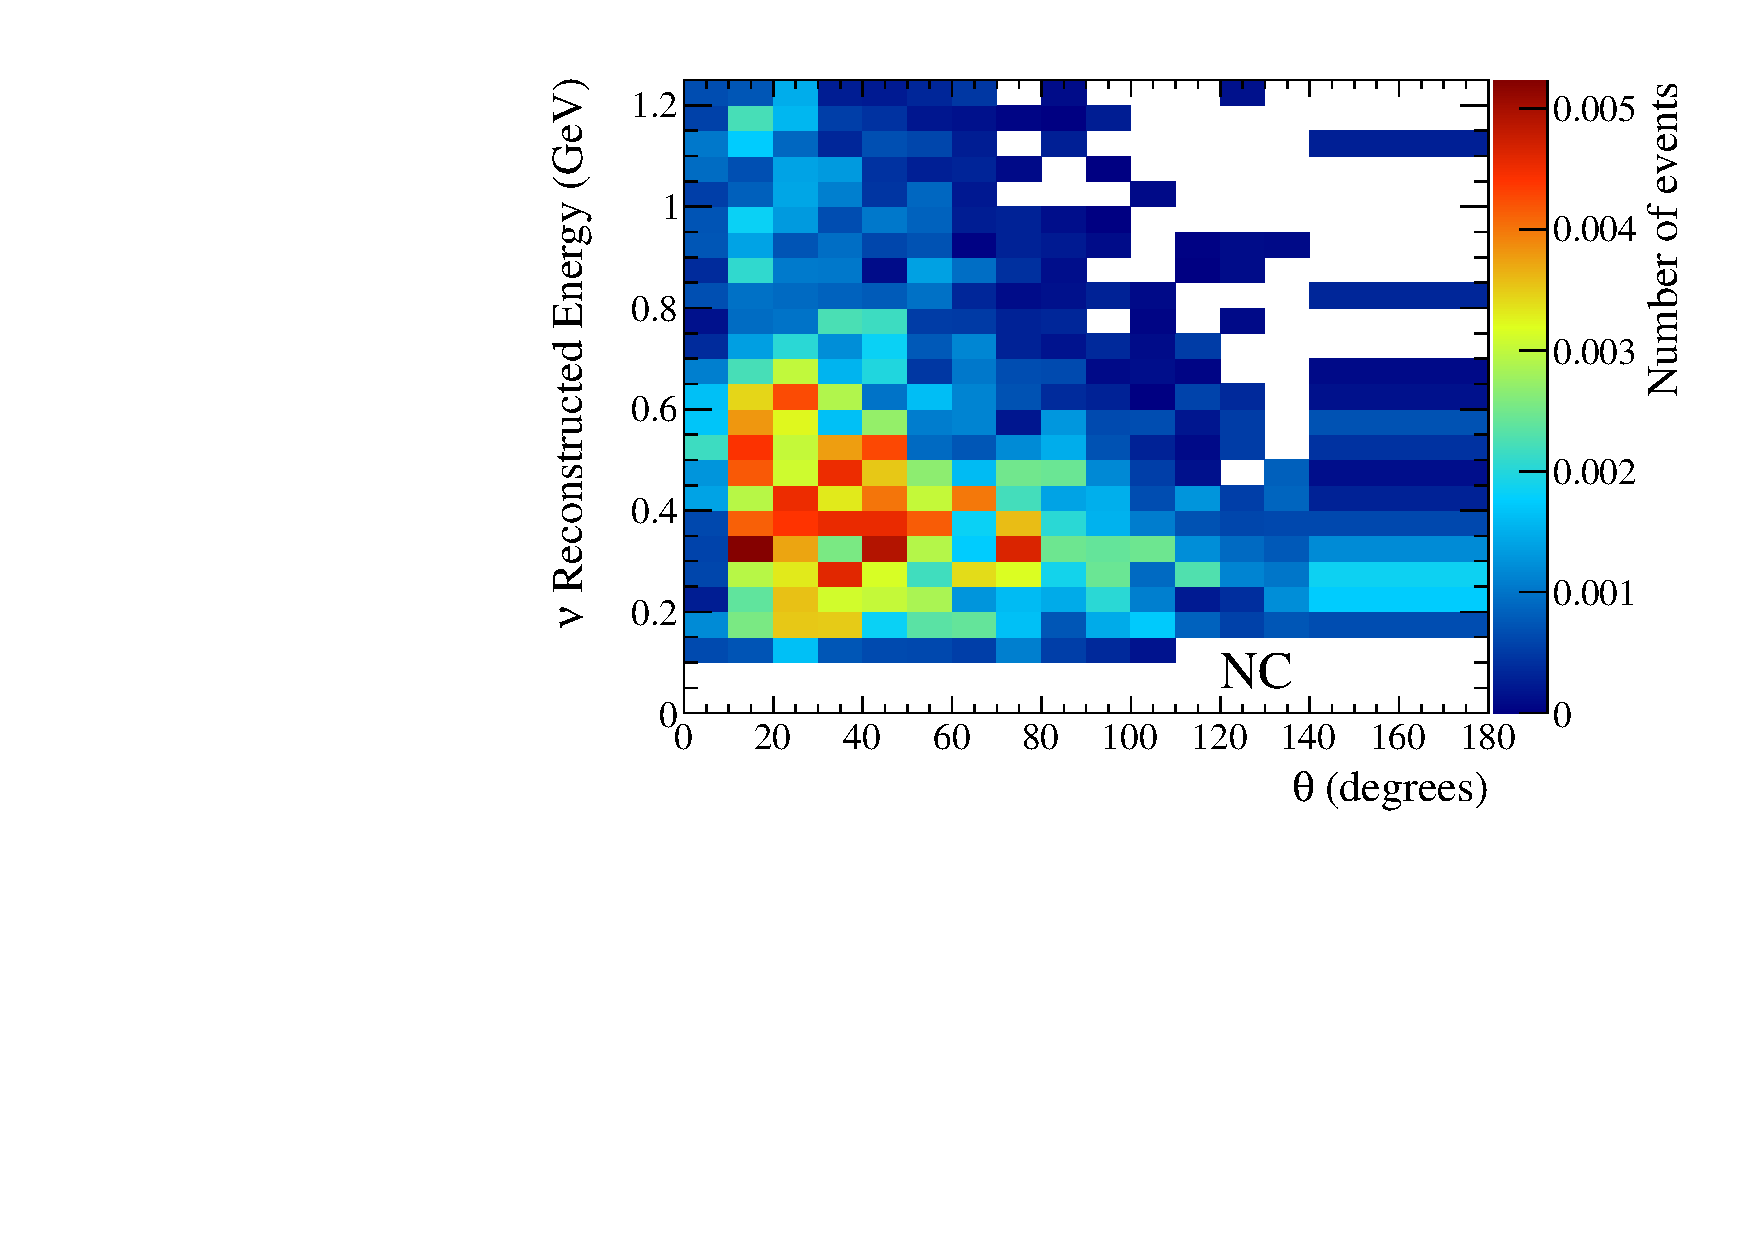
\includegraphics[width=0.9\textwidth]{joint_plots/spectrum_predictions/template_ereco_vs_theta_nc_rhc1re.pdf}
\caption{Neutral current.}
\end{subfigure}
\begin{subfigure}[b]{0.49\textwidth}
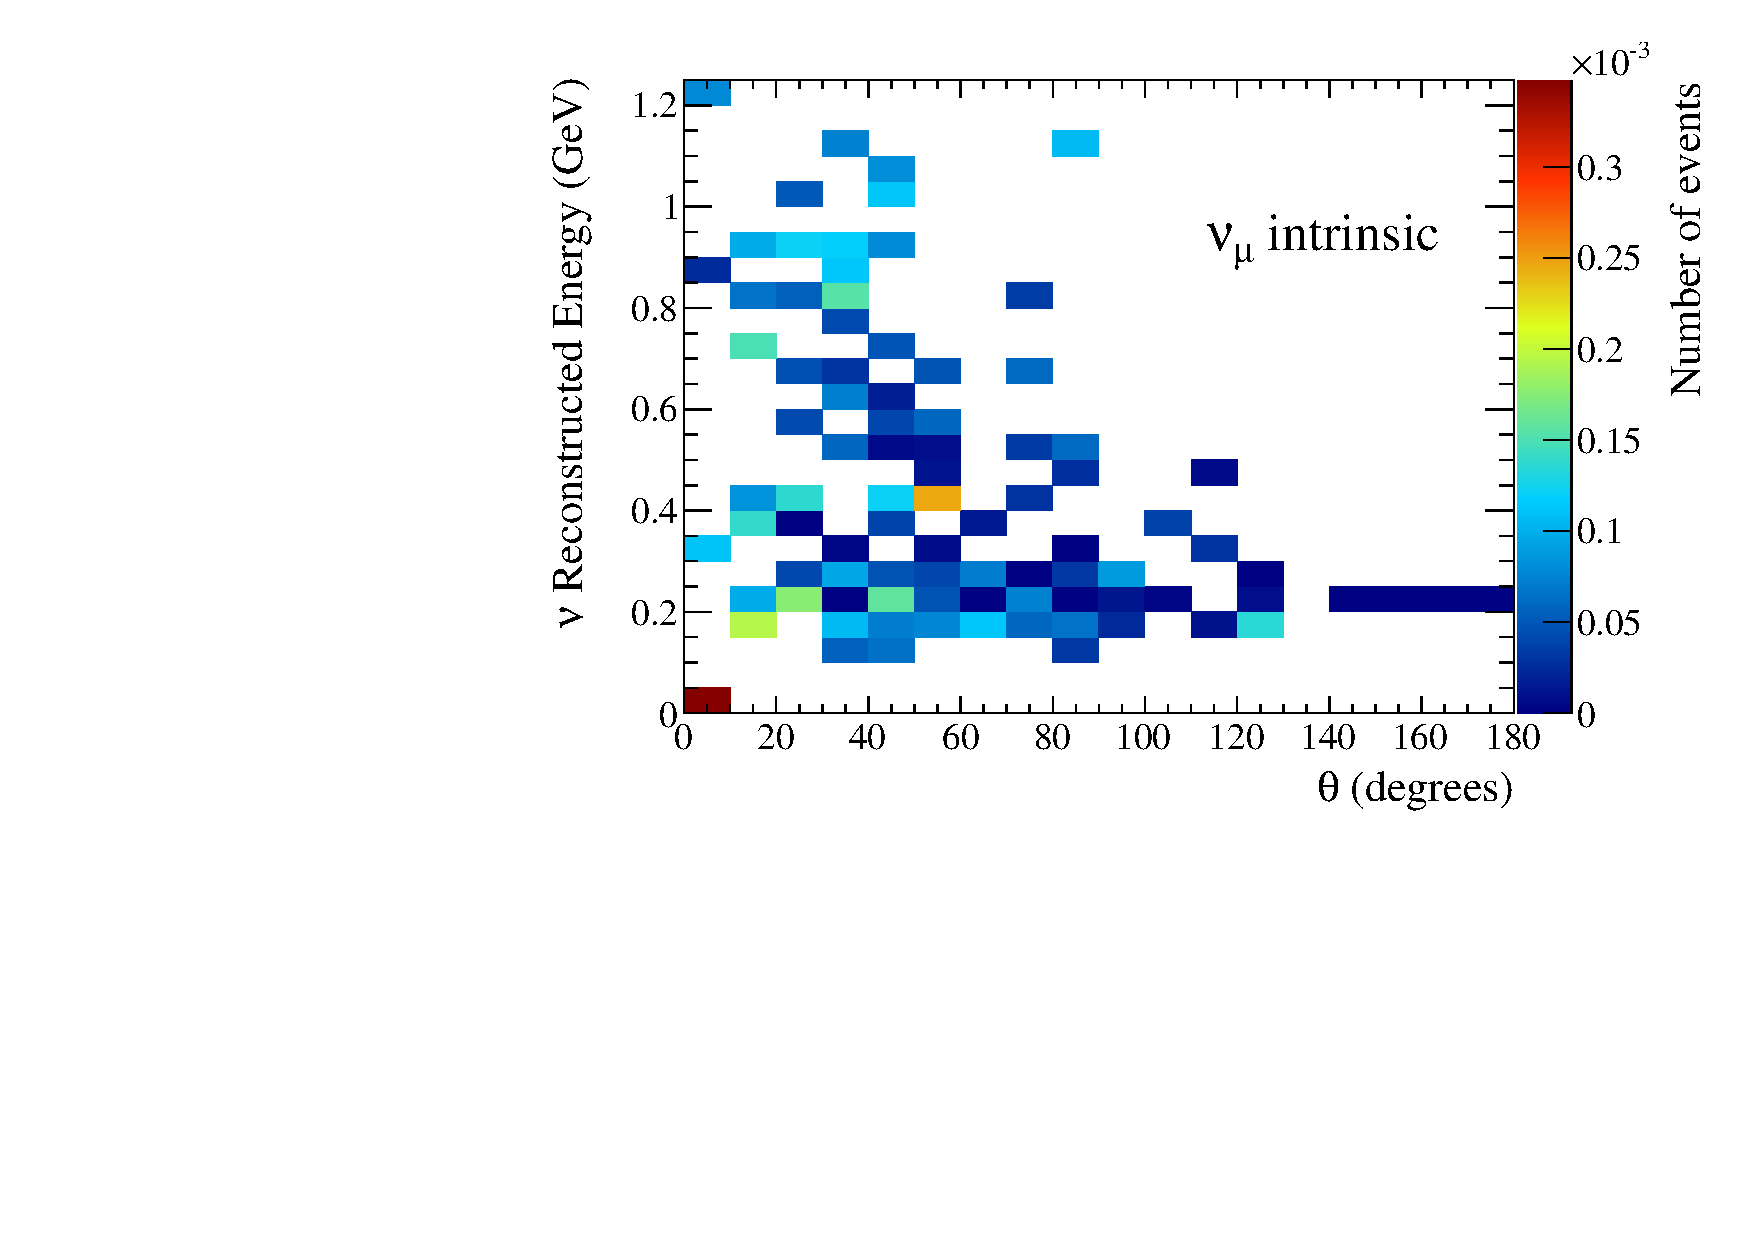
\includegraphics[width=0.9\textwidth]{joint_plots/spectrum_predictions/template_ereco_vs_theta_numubeam_rhc1re.pdf}
\caption{$\nu_{\mu}$ intrinsic beam.}
\end{subfigure}
\begin{subfigure}[b]{0.49\textwidth}
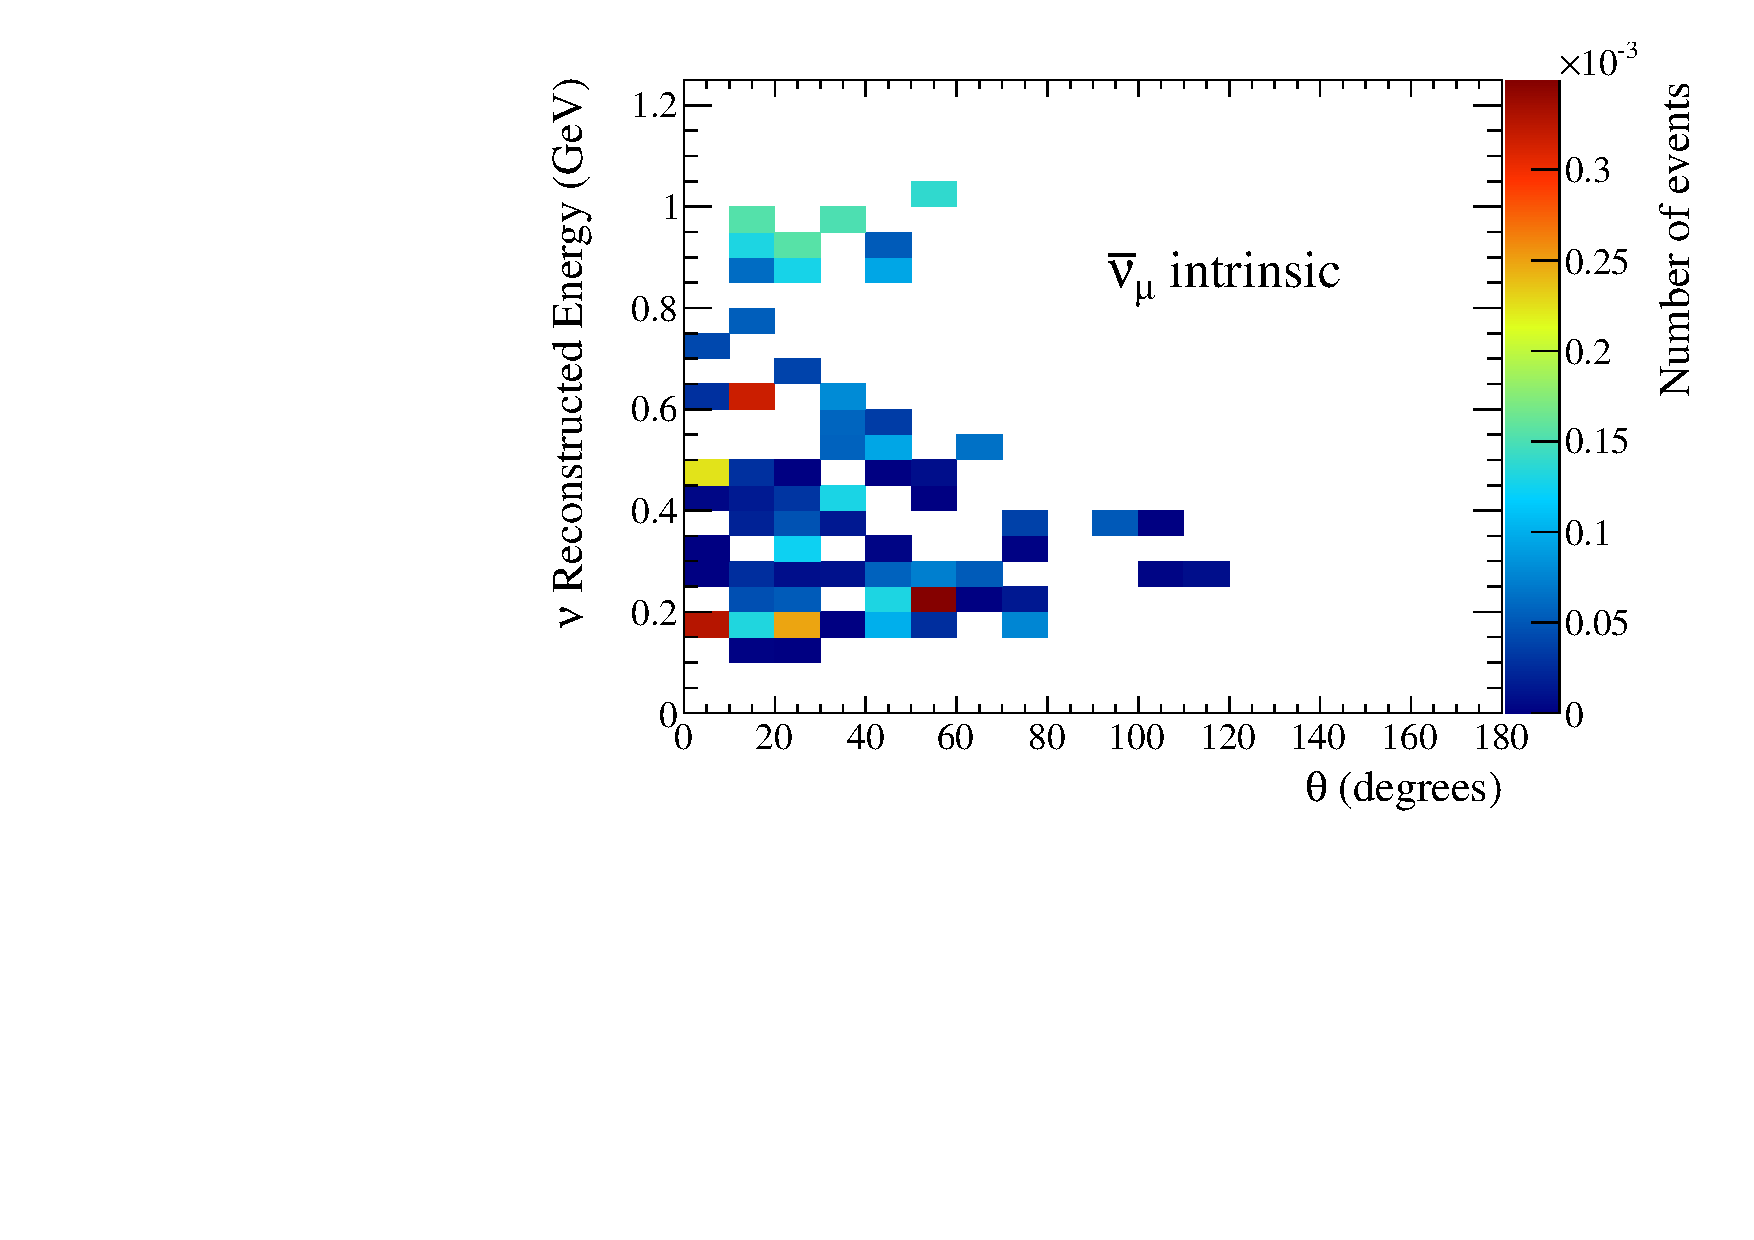
\includegraphics[width=0.9\textwidth]{joint_plots/spectrum_predictions/template_ereco_vs_theta_numubarbeam_rhc1re.pdf}
\caption{$\bar{\nu}_{\mu}$ intrinsic beam.}
\end{subfigure}
\caption {
Predicted spectra of electron-like events
as a function of the reconstructed neutrino energy and
the angle between the outgoing lepton and the neutrino direction.
The distributions correspond to the collected statistics in the full Run 1-6 data set
for an exposure.
%of $6.914 \times 10^{20}$ POT in neutrino  mode.
%and
%of $4.011 \times 10^{20}$ POT in antineutrino mode.
From top left to bottom right the following components are shown:
total,
$\nu_{\mu} \rightarrow \nu_e$,
$\bar{\nu}_{\mu} \rightarrow \bar{\nu}_e$,
$\nu_e + \bar{\nu}_e$ intrinsic beam,
NC,
$\nu_{\mu}$ intrinsic beam
and
$\bar{\nu}_{\mu}$ intrinsic beam.
The spectra were generated with the systematic parameters measured with the ND280 data 
shown in \cref{tab:banff_uncertainties_flux_fhc},~\ref{tab:banff_uncertainties_flux_rhc},~\ref{tab:banff_uncertainties_xsec},
the nominal Super-K systematic parameters shown in \cref{tab:banff_uncertainties_skdetfsi}
and the oscillation parameters corresponding to the Asimov data set A shown in \cref{tab:osc_params_joint_asimov}.
}
\label{fig:joint_ereco_vs_theta_rhc1re}
\end{figure*}


In \cref{fig:joint_1d_elike} the projection of the 2-dimensional $e$-like templates
onto the $E_{reco}$ and $\theta$ axes are shown.

\begin{figure*}[htb]
%\hspace{0.06\linewidth}
\center
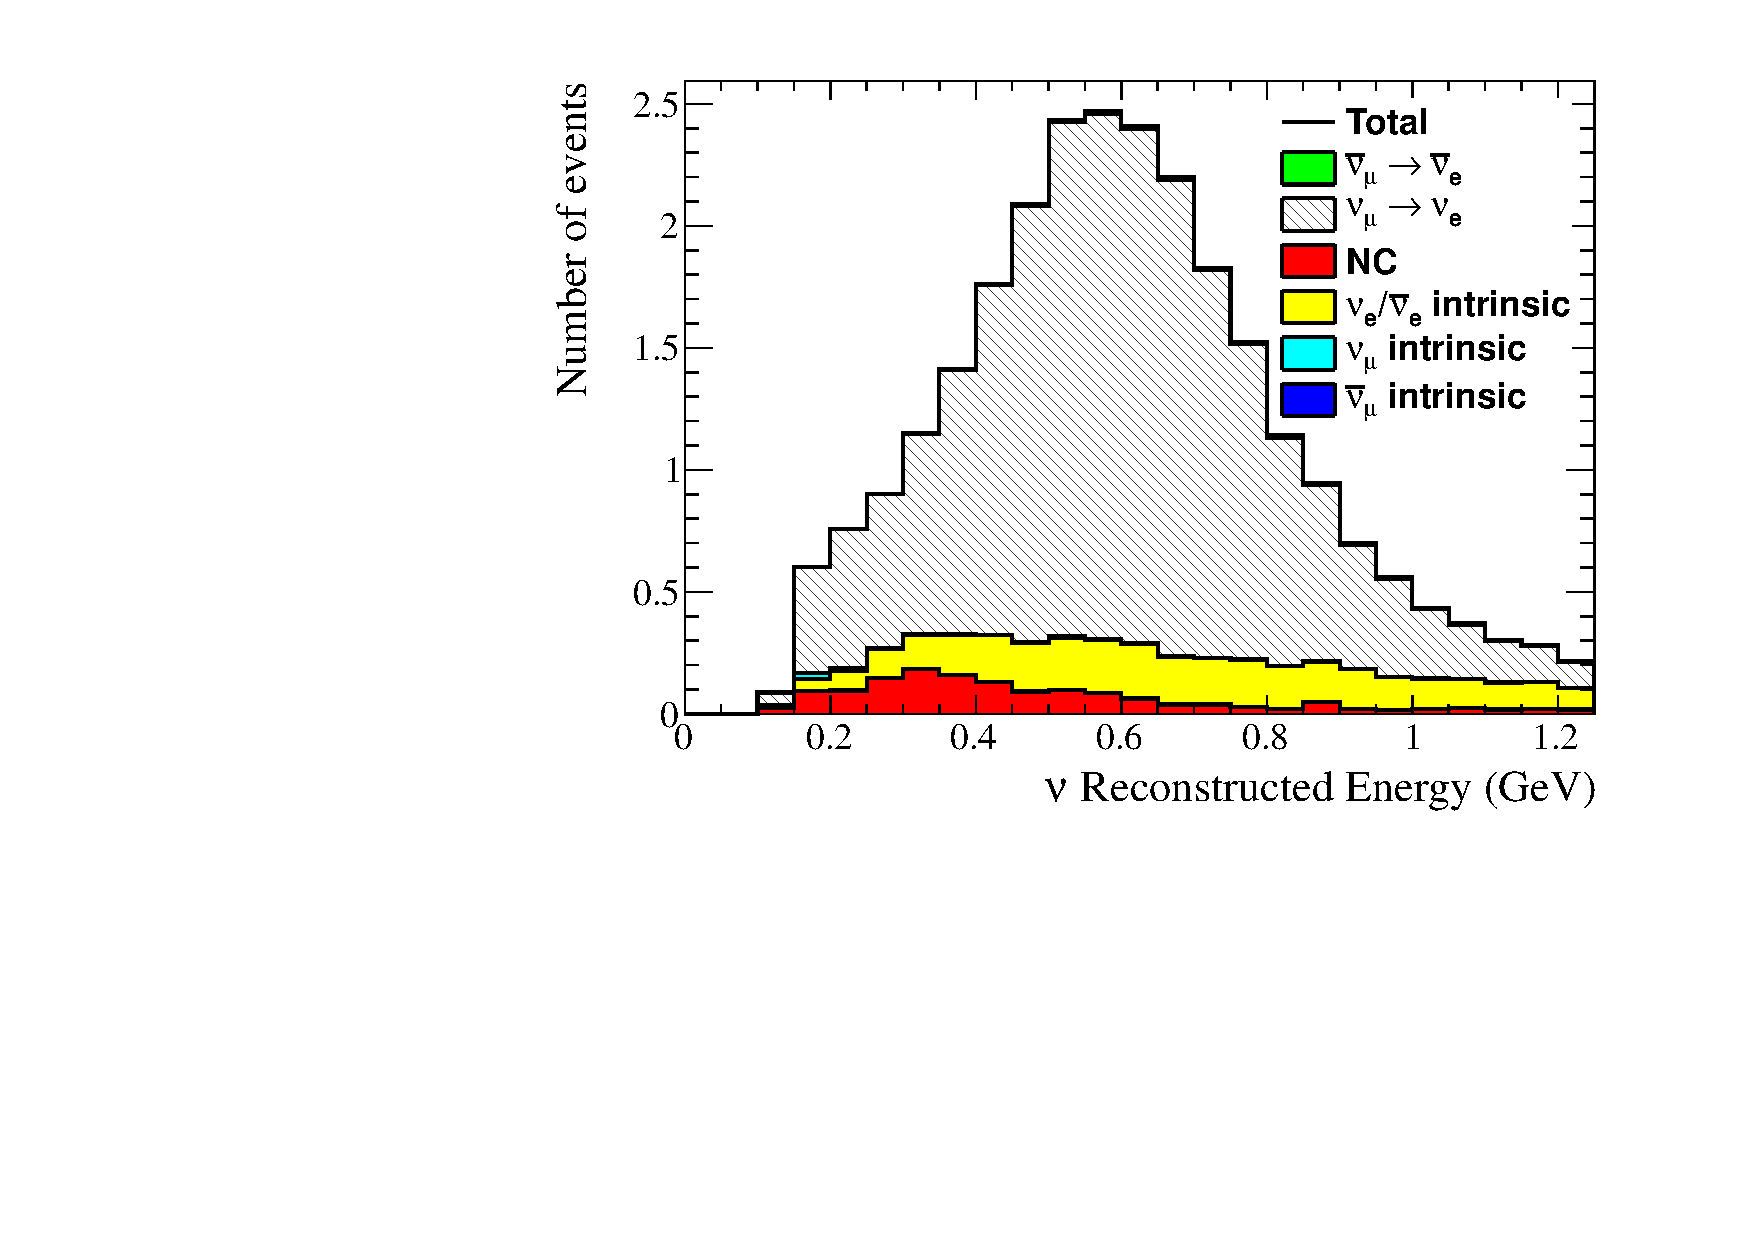
\includegraphics[width=18pc]{joint_plots/spectrum_predictions/template_ereco_1re.pdf}
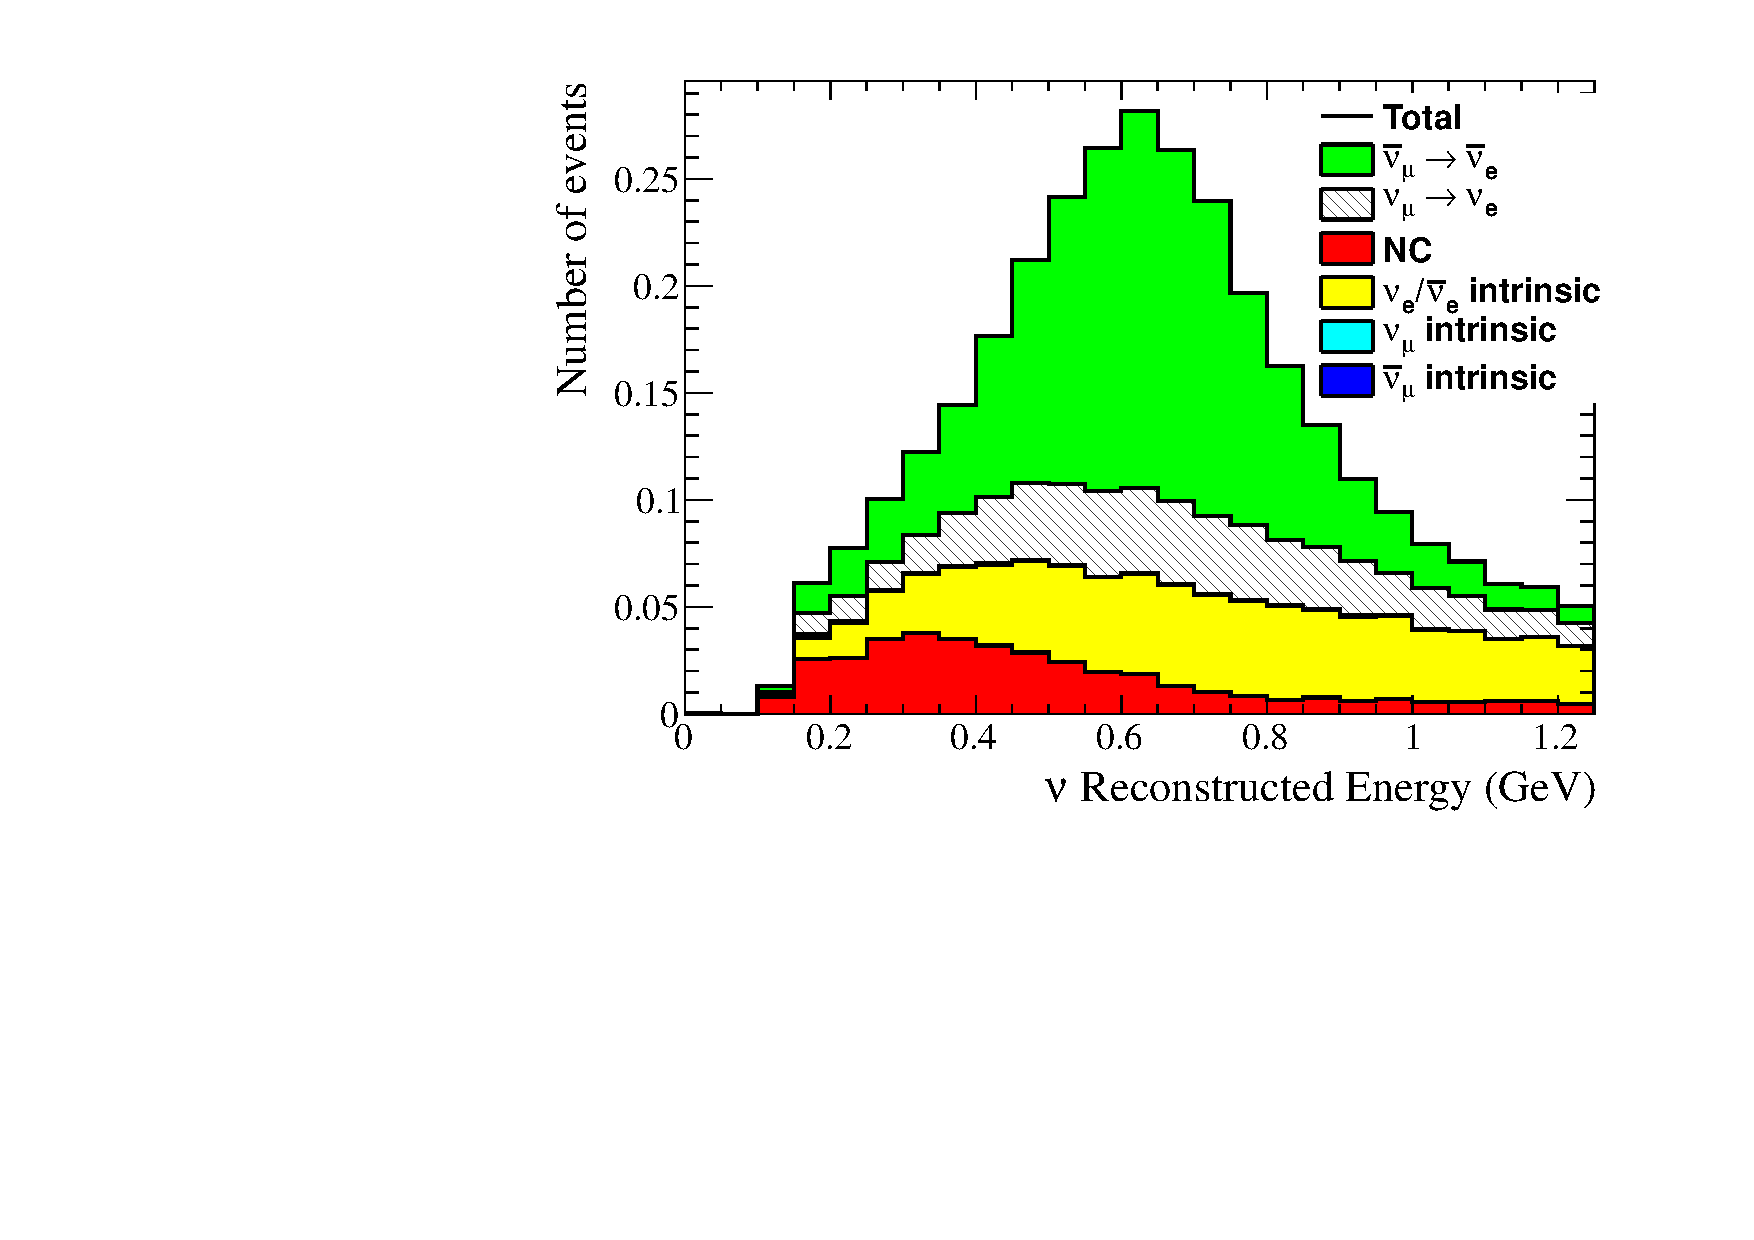
\includegraphics[width=18pc]{joint_plots/spectrum_predictions/template_ereco_rhc1re.pdf}
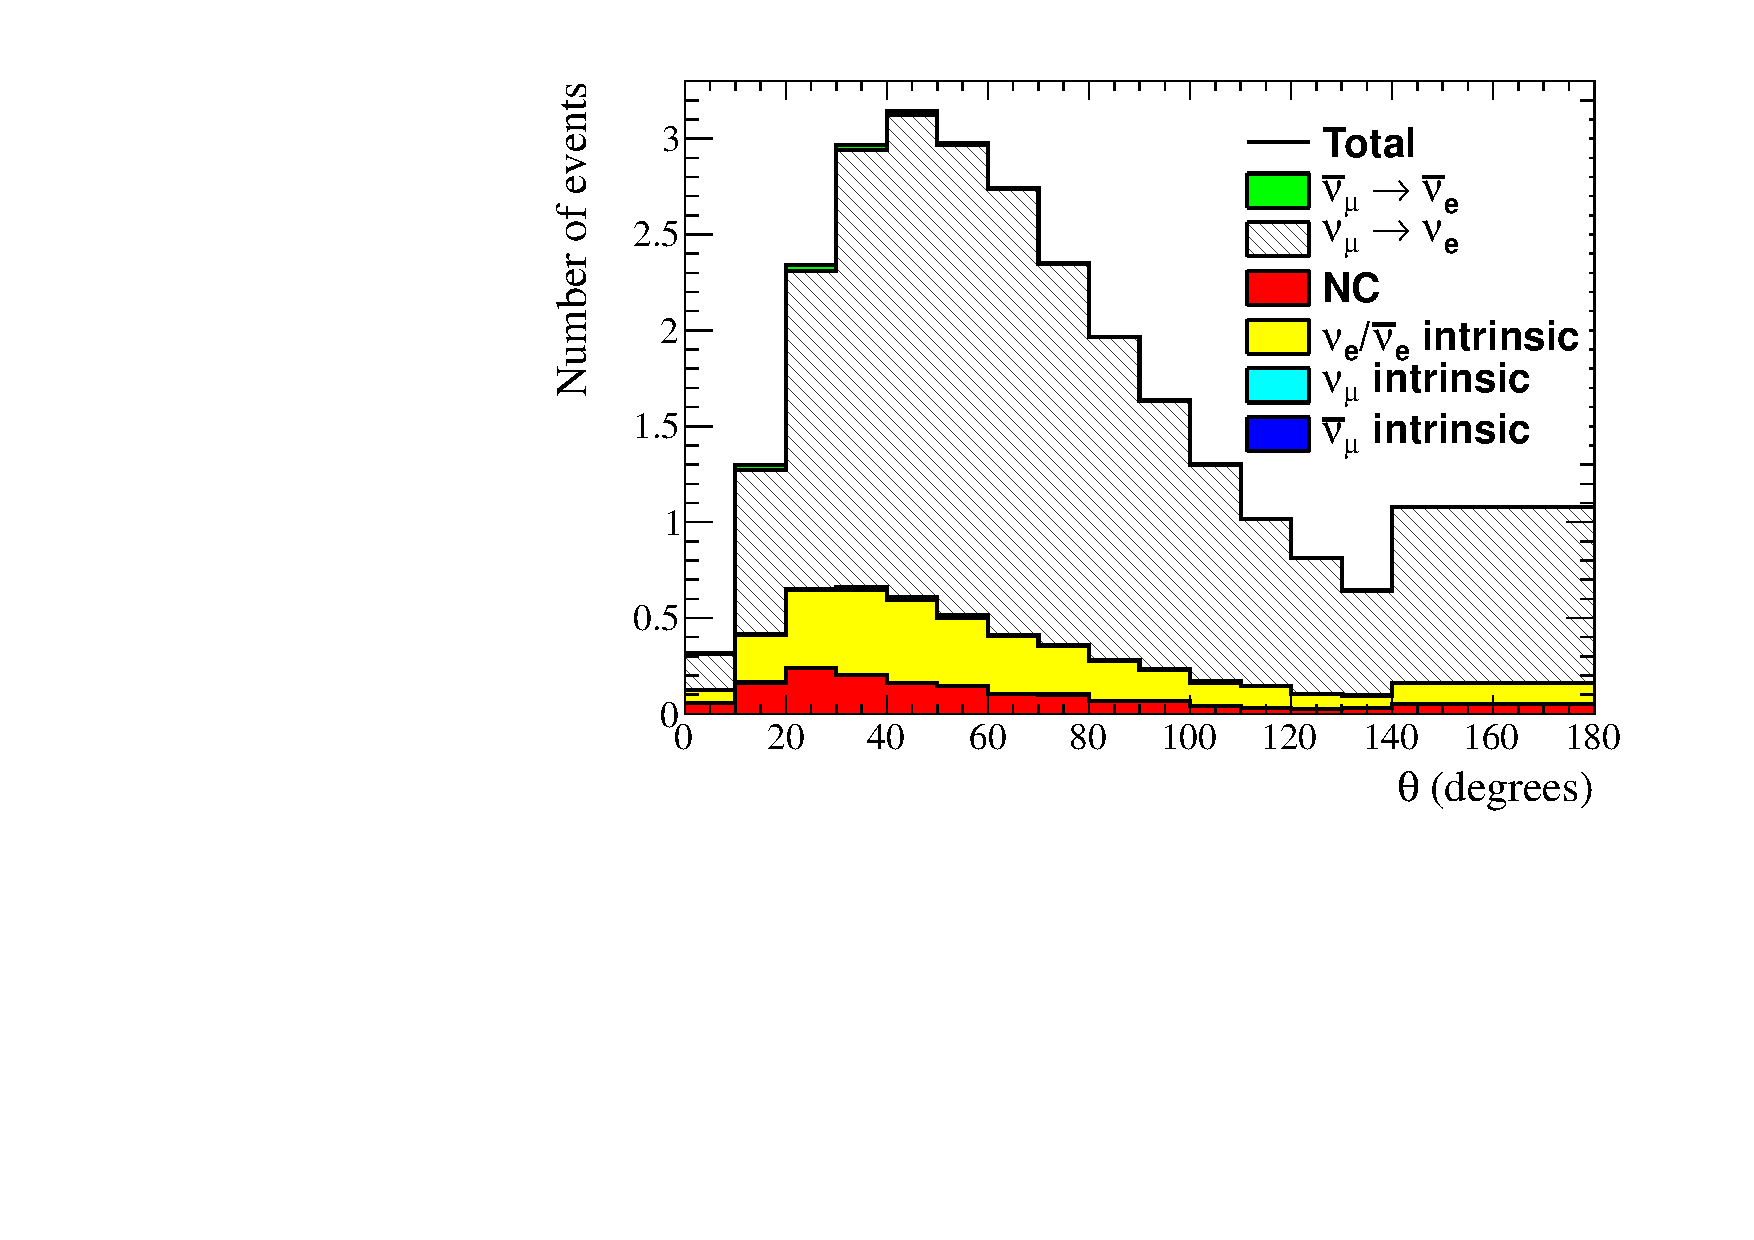
\includegraphics[width=18pc]{joint_plots/spectrum_predictions/template_theta_1re.pdf}
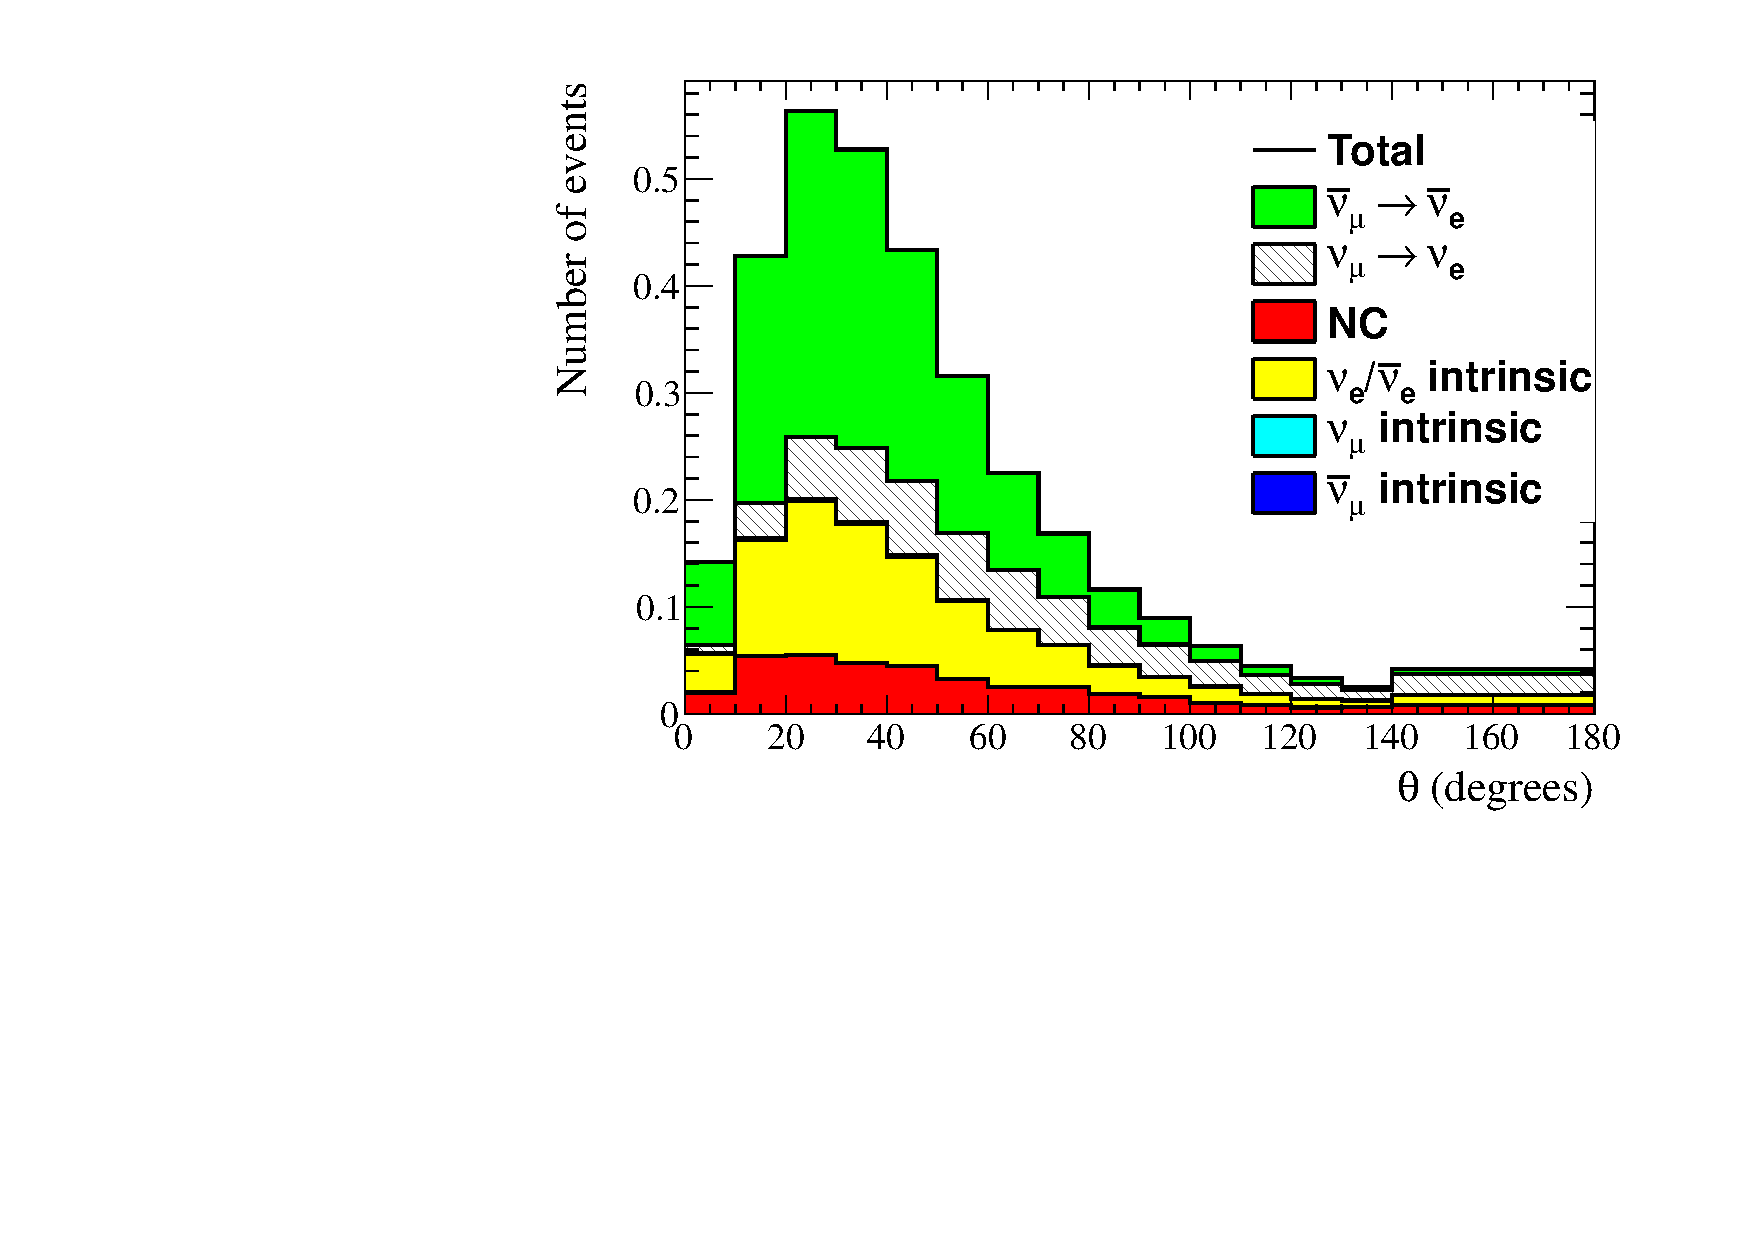
\includegraphics[width=18pc]{joint_plots/spectrum_predictions/template_theta_rhc1re.pdf}
\caption {
Predicted spectra of 
the reconstructed neutrino energy (top) 
and
the angle between the neutrino and the outgoing lepton directions (bottom)
for electron-like 
neutrino mode (left)
and
antineutrino mode (right)
events.
The distributions correspond to the collected statistics in the full Run 1-6 data set.
%for an exposure 
%of $6.914 \times 10^{20}$ POT in neutrino mode
%and
%of $4.011 \times 10^{20}$ POT in antineutrino mode.
The distributions are broken down by the following components:
$\bar{\nu}_{\mu} \to \bar{\nu}_e$ (green), 
$\nu_{\mu} \to \nu_e$ (black/white), 
NC (red),
$\nu_e + \bar{\nu}_e$ intrinsic beam (yellow),
$\nu_{\mu}$ intrinsic beam (light blue)
and
$\bar{\nu}_{\mu}$ intrinsic beam (blue).
The spectra were generated with the systematic parameters measured with the ND280 data 
shown in \cref{tab:banff_uncertainties_flux_fhc},~\ref{tab:banff_uncertainties_flux_rhc},~\ref{tab:banff_uncertainties_xsec},
the nominal Super-K systematic parameters shown in \cref{tab:banff_uncertainties_skdetfsi}
and the oscillation parameters corresponding to the Asimov data set A shown in \cref{tab:osc_params_joint_asimov}.
}
\label{fig:joint_1d_elike}
\end{figure*}


%\clearpage


\clearpage


%...........................................................
%
% Observed spectra
%
%...........................................................

\section{Observed $e$-like spectra}
\label{app:templates_observed}

In \cref{fig:joint_ereco_vs_theta_1re_data} and~\ref{fig:joint_ereco_vs_theta_rhc1re_data}
the predicted breakdown of the $e$-like 2-dimensional spectra are compared to data for
both neutrino and antineutrino beam mode.

\begin{figure*}[htb]
\center
\begin{subfigure}[b]{0.49\textwidth}
\includegraphics[width=0.9\textwidth]{./joint_plots/data/data_mc_1re_2d_NuMuToNue.pdf}
\caption{$\nu_{\mu} \rightarrow \nu_e$.}
\end{subfigure}
\begin{subfigure}[b]{0.49\textwidth}
\includegraphics[width=0.9\textwidth]{./joint_plots/data/data_mc_1re_2d_NuMuBarToNueBar.pdf}
\caption{$\bar{\nu}_{\mu} \rightarrow \bar{\nu}_e$.}
\end{subfigure}
\begin{subfigure}[b]{0.49\textwidth}
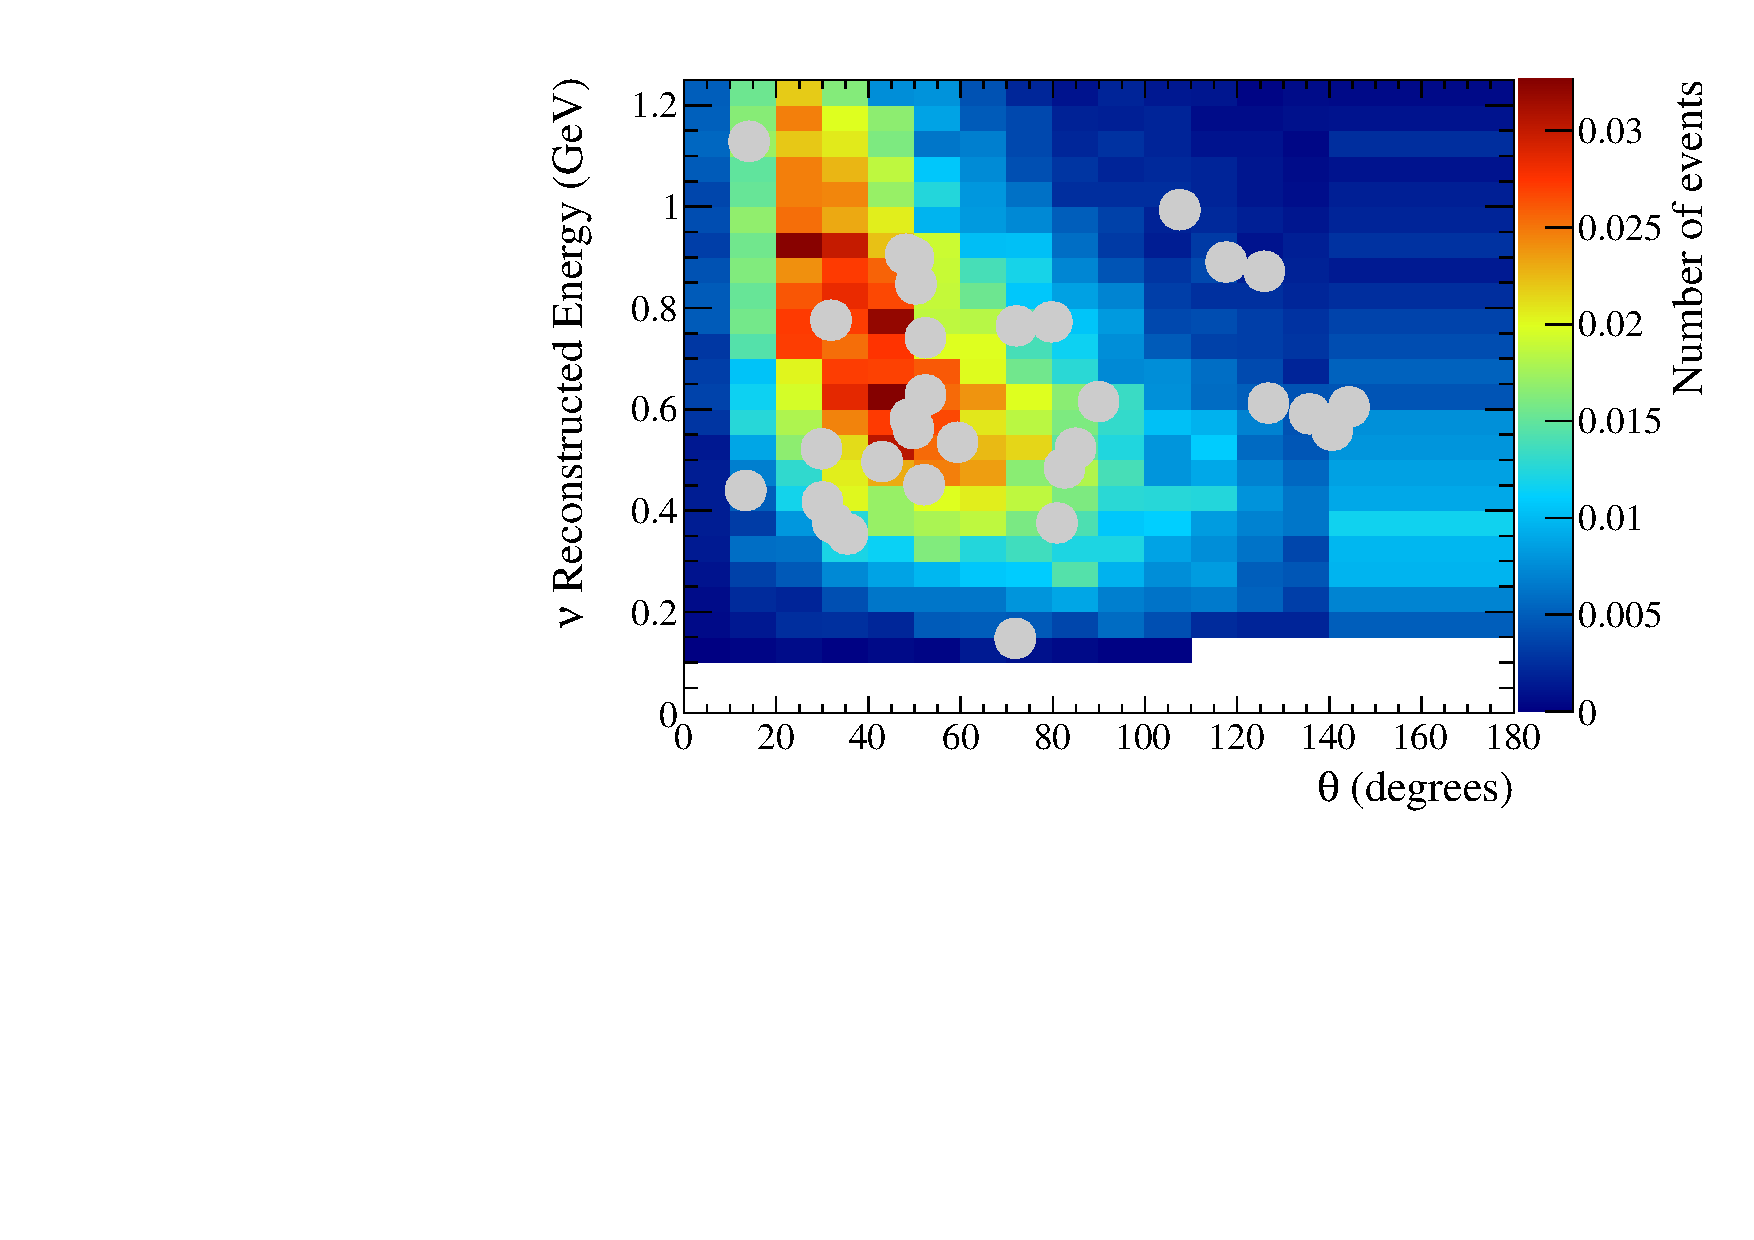
\includegraphics[width=0.9\textwidth]{./joint_plots/data/data_mc_1re_2d_NueBeam.pdf}
\caption{$\nu_{e}$ + $\bar{\nu}_e$ intrinsic beam.}
\end{subfigure}
\begin{subfigure}[b]{0.49\textwidth}
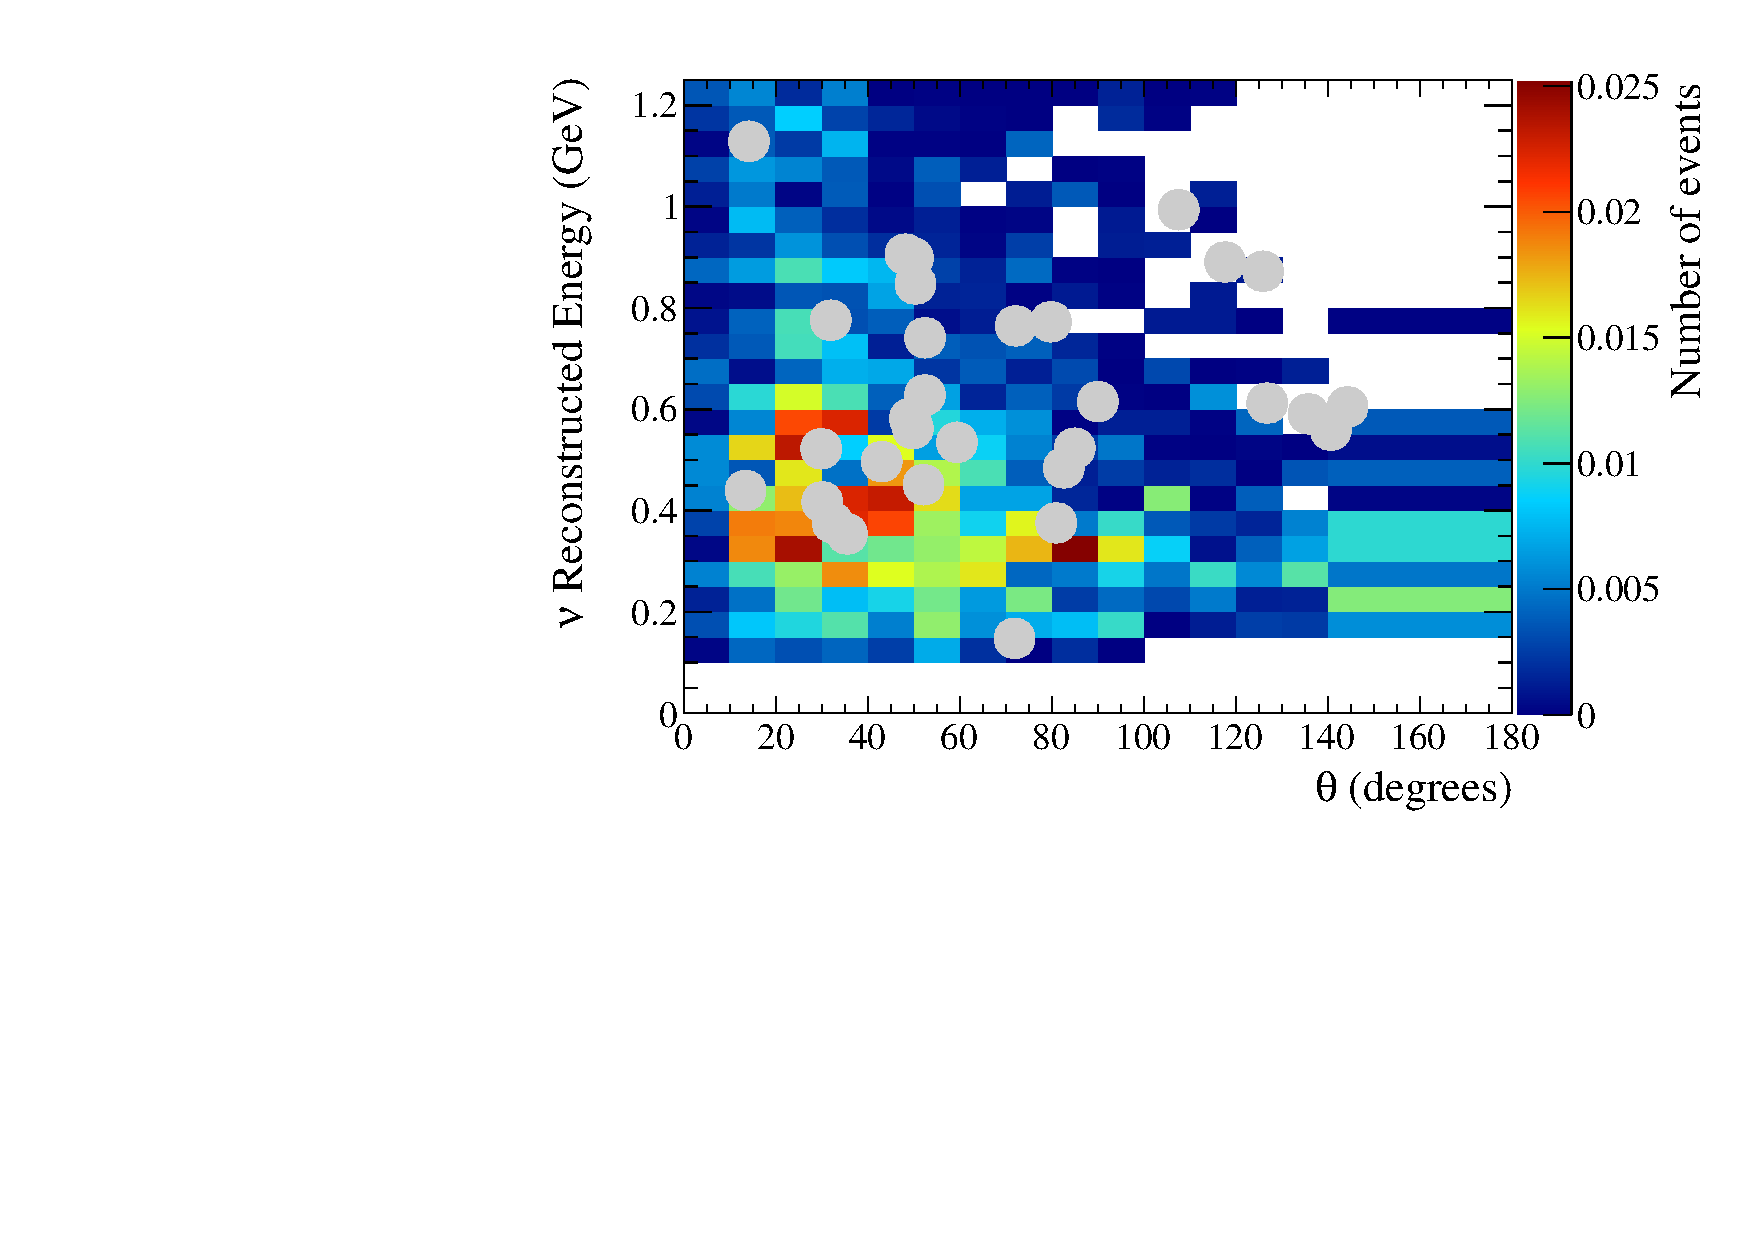
\includegraphics[width=0.9\textwidth]{./joint_plots/data/data_mc_1re_2d_NC.pdf}
\caption{Neutral current.}
\end{subfigure}
\begin{subfigure}[b]{0.49\textwidth}
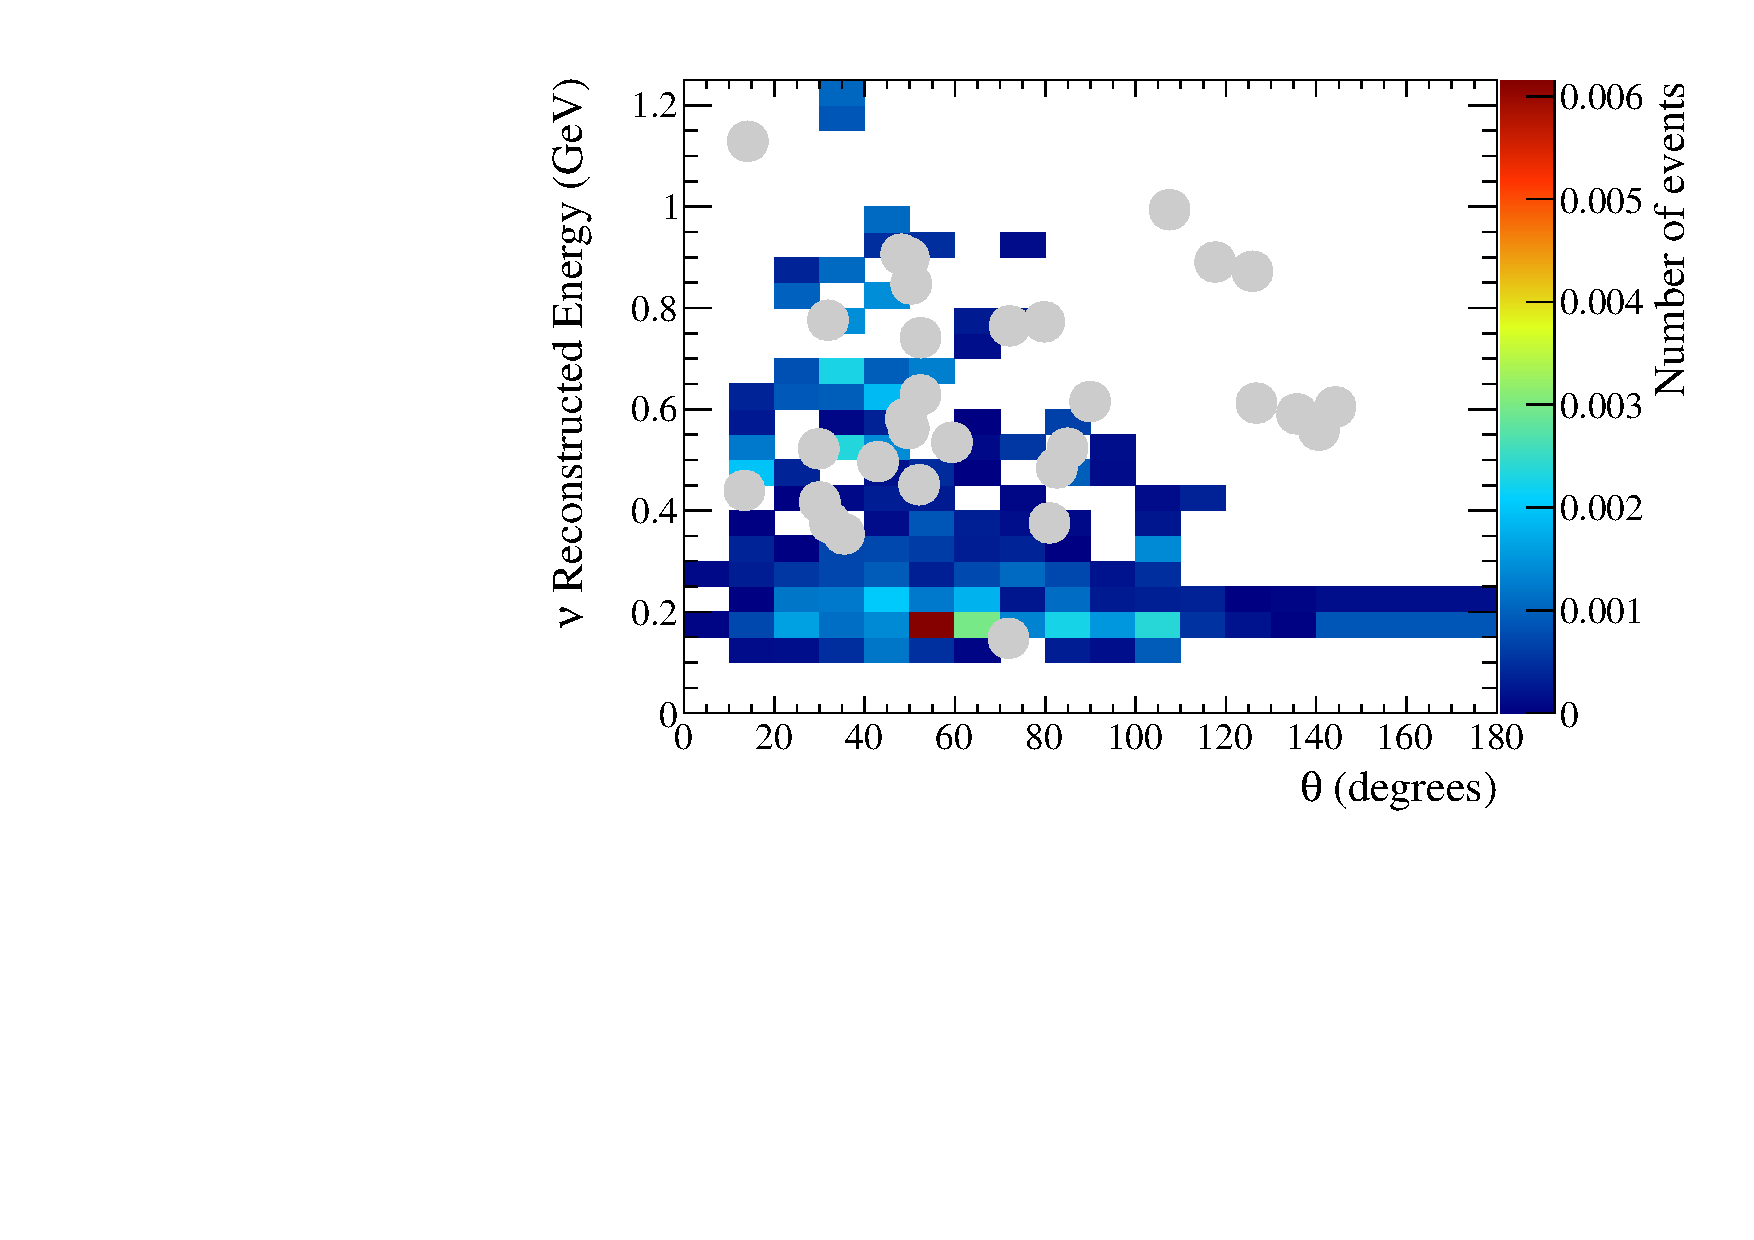
\includegraphics[width=0.9\textwidth]{./joint_plots/data/data_mc_1re_2d_NumuBeam.pdf}
\caption{$\nu_{\mu}$ intrinsic beam.}
\end{subfigure}
\begin{subfigure}[b]{0.49\textwidth}
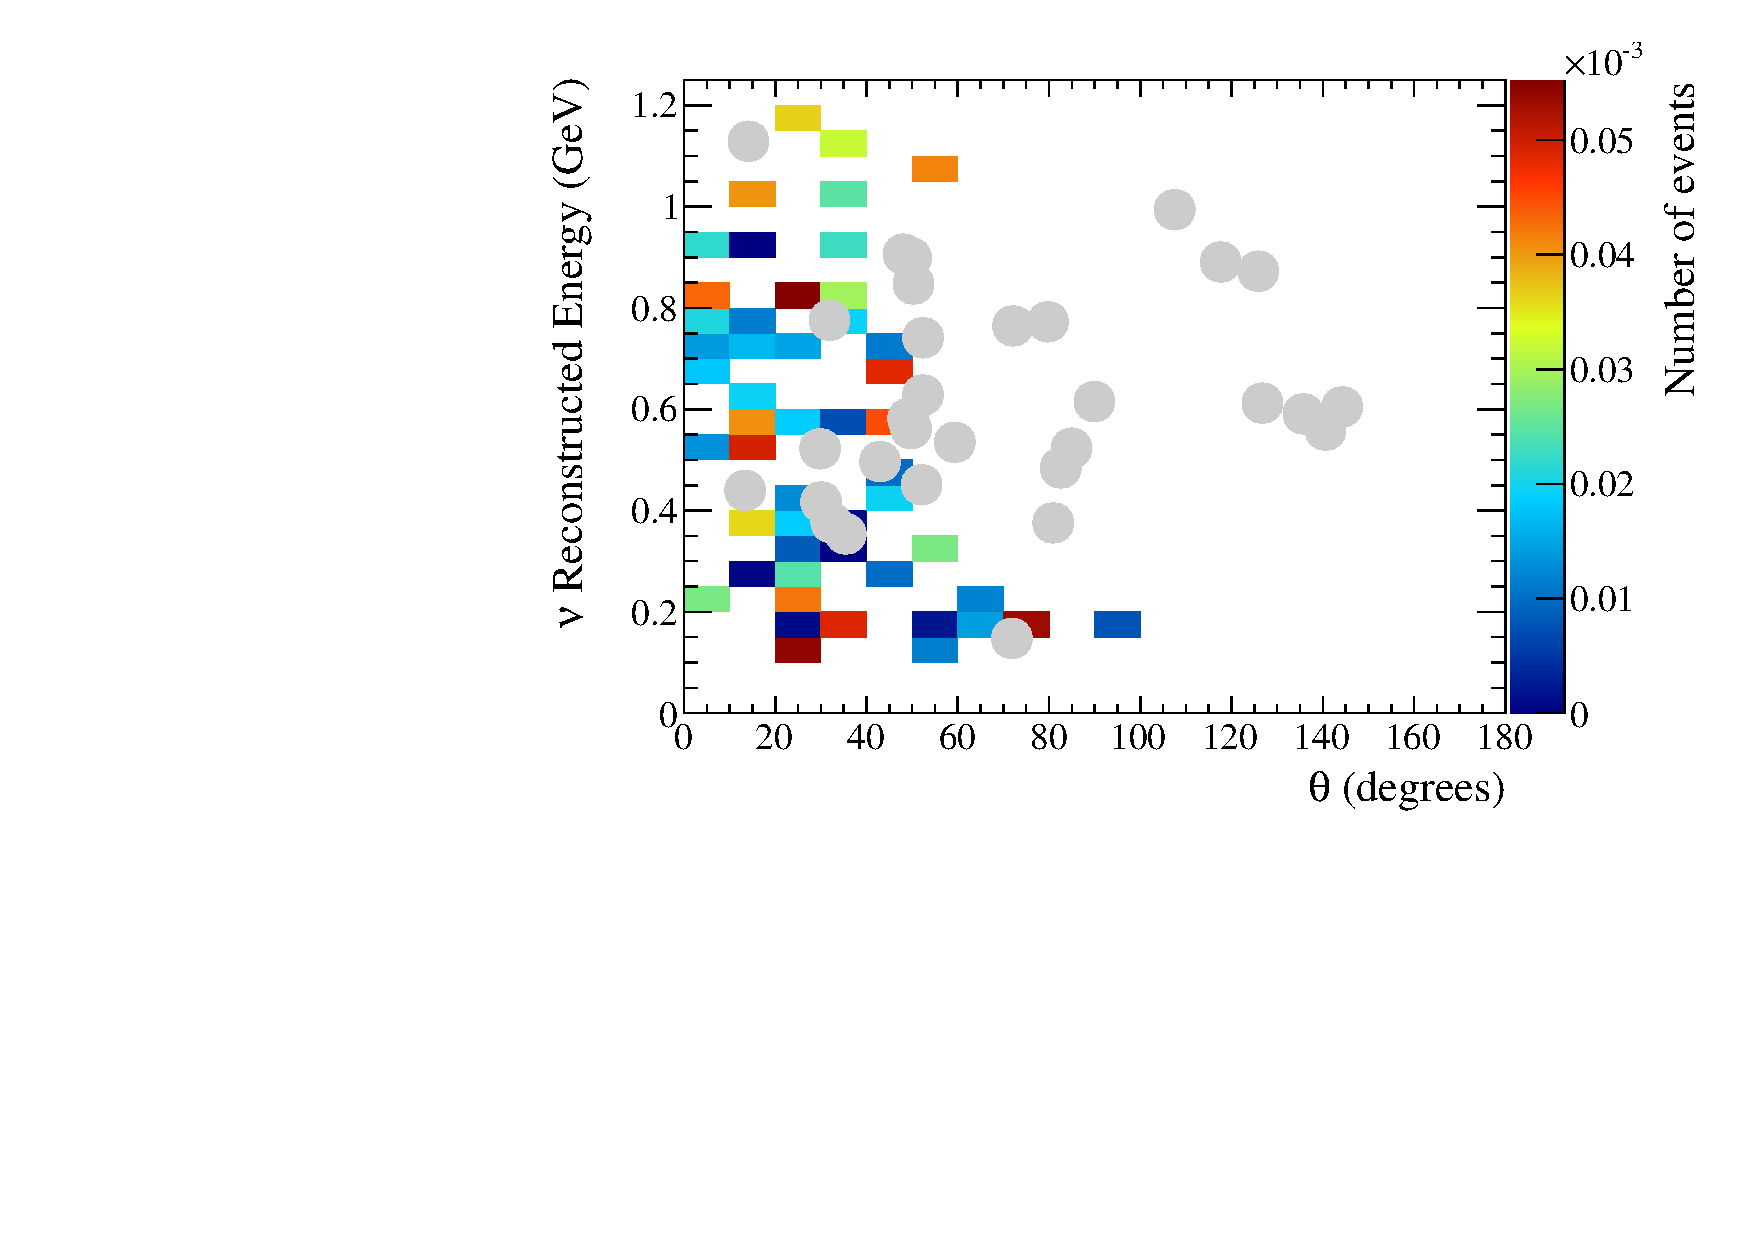
\includegraphics[width=0.9\textwidth]{./joint_plots/data/data_mc_1re_2d_NumuBarBeam.pdf}
\caption{$\bar{\nu}_{\mu}$ intrinsic beam.}
\end{subfigure}
\caption {
Predicted and observed (grey dots) spectra of electron-like events
as a function of the reconstructed neutrino energy and
the angle between the outgoing lepton and the neutrino direction.
The distributions correspond to the collected statistics in the full Run 1-6 data set.
%for an exposure 
%of $6.914 \times 10^{20}$ POT in neutrino mode.
%and
%of $4.011 \times 10^{20}$ POT in antineutrino mode.
From top left to bottom right the following components are shown:
%total,
$\nu_{\mu} \rightarrow \nu_e$,
$\bar{\nu}_{\mu} \rightarrow \bar{\nu}_e$,
$\nu_e + \bar{\nu}_e$ intrinsic beam,
NC,
$\nu_{\mu}$ intrinsic beam
and
$\bar{\nu}_{\mu}$ intrinsic beam.
The spectra were generated with the systematic parameters measured with the ND280 data 
shown in \cref{tab:banff_uncertainties_flux_fhc},~\ref{tab:banff_uncertainties_flux_rhc},~\ref{tab:banff_uncertainties_xsec},
the nominal Super-K systematic parameters shown in \cref{tab:banff_uncertainties_skdetfsi}
and the oscillation parameters corresponding to the Asimov data set A shown in \cref{tab:osc_params_joint_asimov}.
}
\label{fig:joint_ereco_vs_theta_1re_data}
\end{figure*}

\begin{figure*}[htb]
\center
\begin{subfigure}[b]{0.49\textwidth}
\includegraphics[width=0.9\textwidth]{./joint_plots/data/data_mc_rhc1re_2d_NuMuToNue.pdf}
\caption{$\nu_{\mu} \rightarrow \nu_e$.}
\end{subfigure}
\begin{subfigure}[b]{0.49\textwidth}
\includegraphics[width=0.9\textwidth]{./joint_plots/data/data_mc_rhc1re_2d_NuMuBarToNueBar.pdf}
\caption{$\bar{\nu}_{\mu} \rightarrow \bar{\nu}_e$.}
\end{subfigure}
\begin{subfigure}[b]{0.49\textwidth}
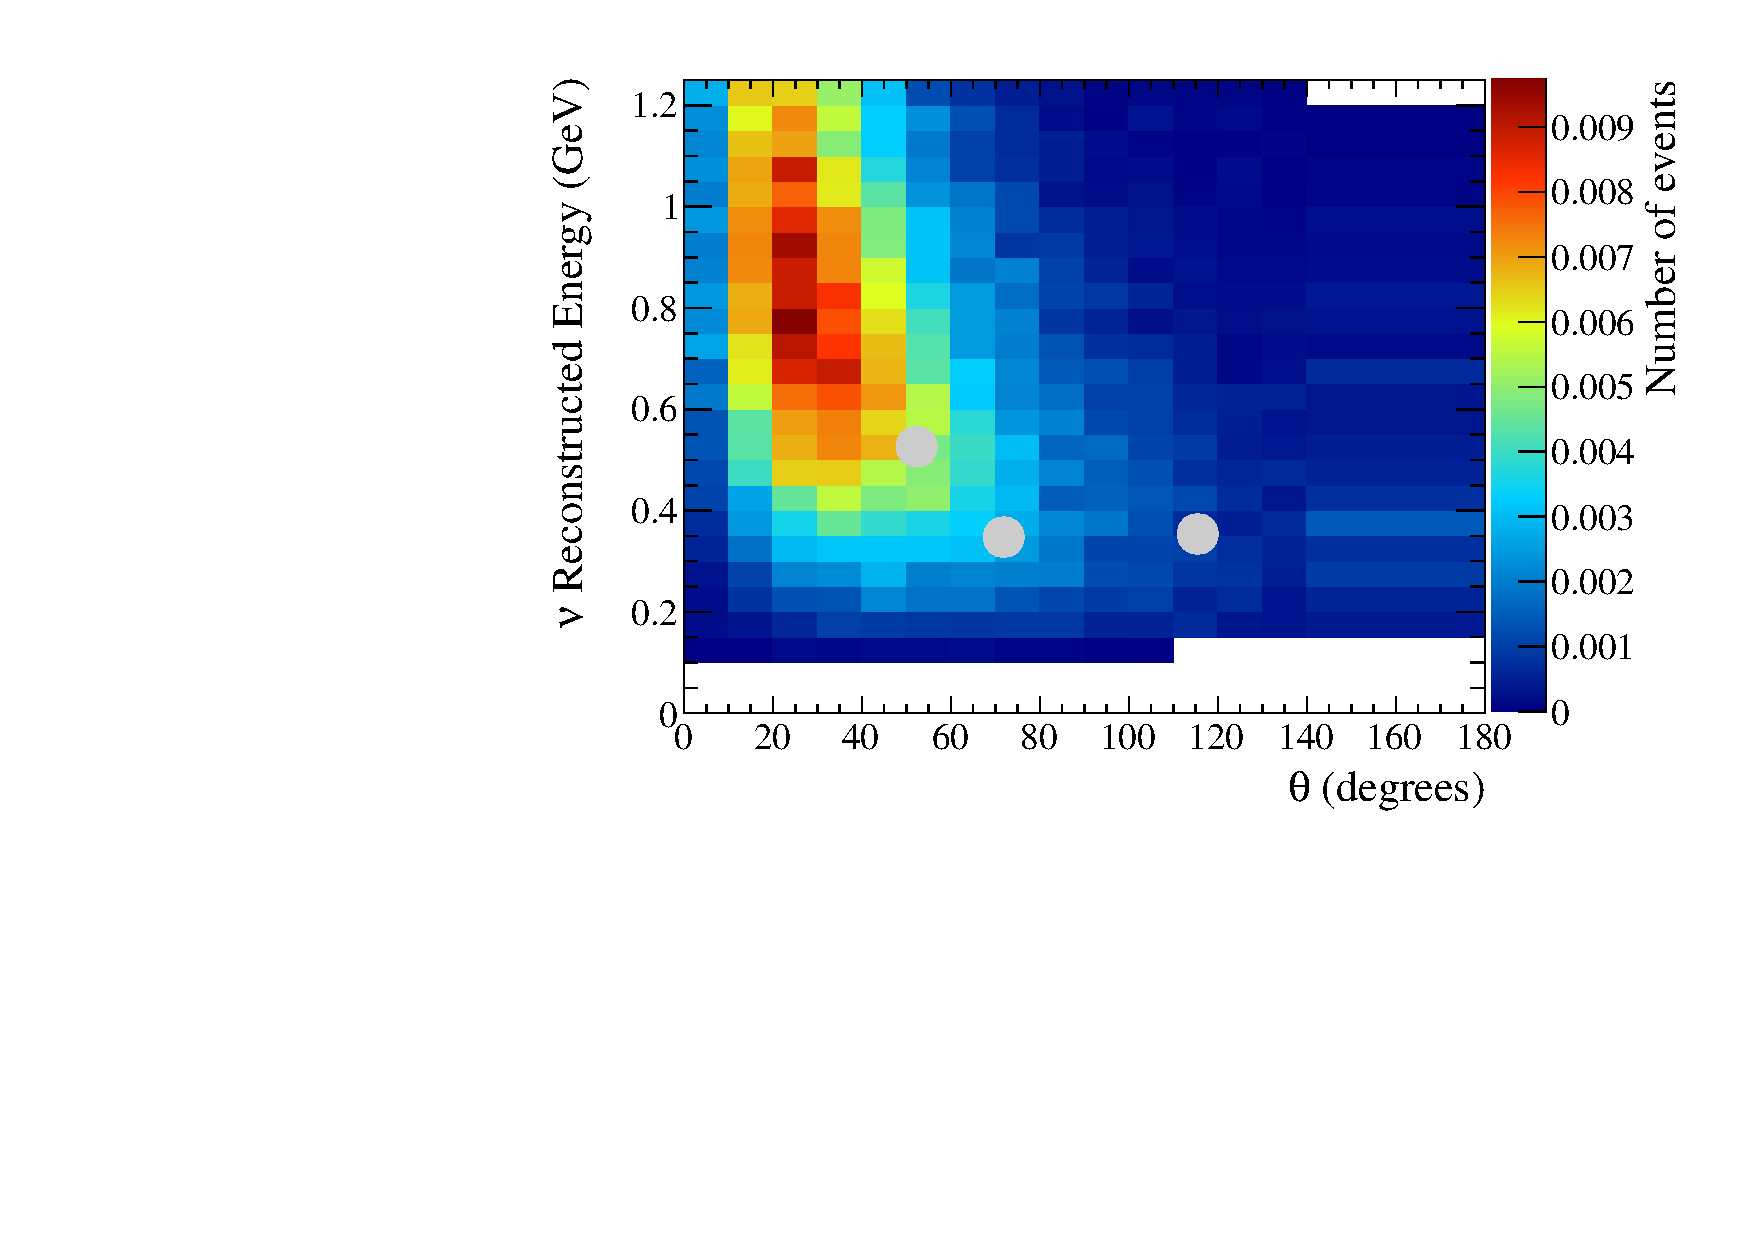
\includegraphics[width=0.9\textwidth]{./joint_plots/data/data_mc_rhc1re_2d_NueBeam.pdf}
\caption{$\nu_{e}$ + $\bar{\nu}_e$ intrinsic beam.}
\end{subfigure}
\begin{subfigure}[b]{0.49\textwidth}
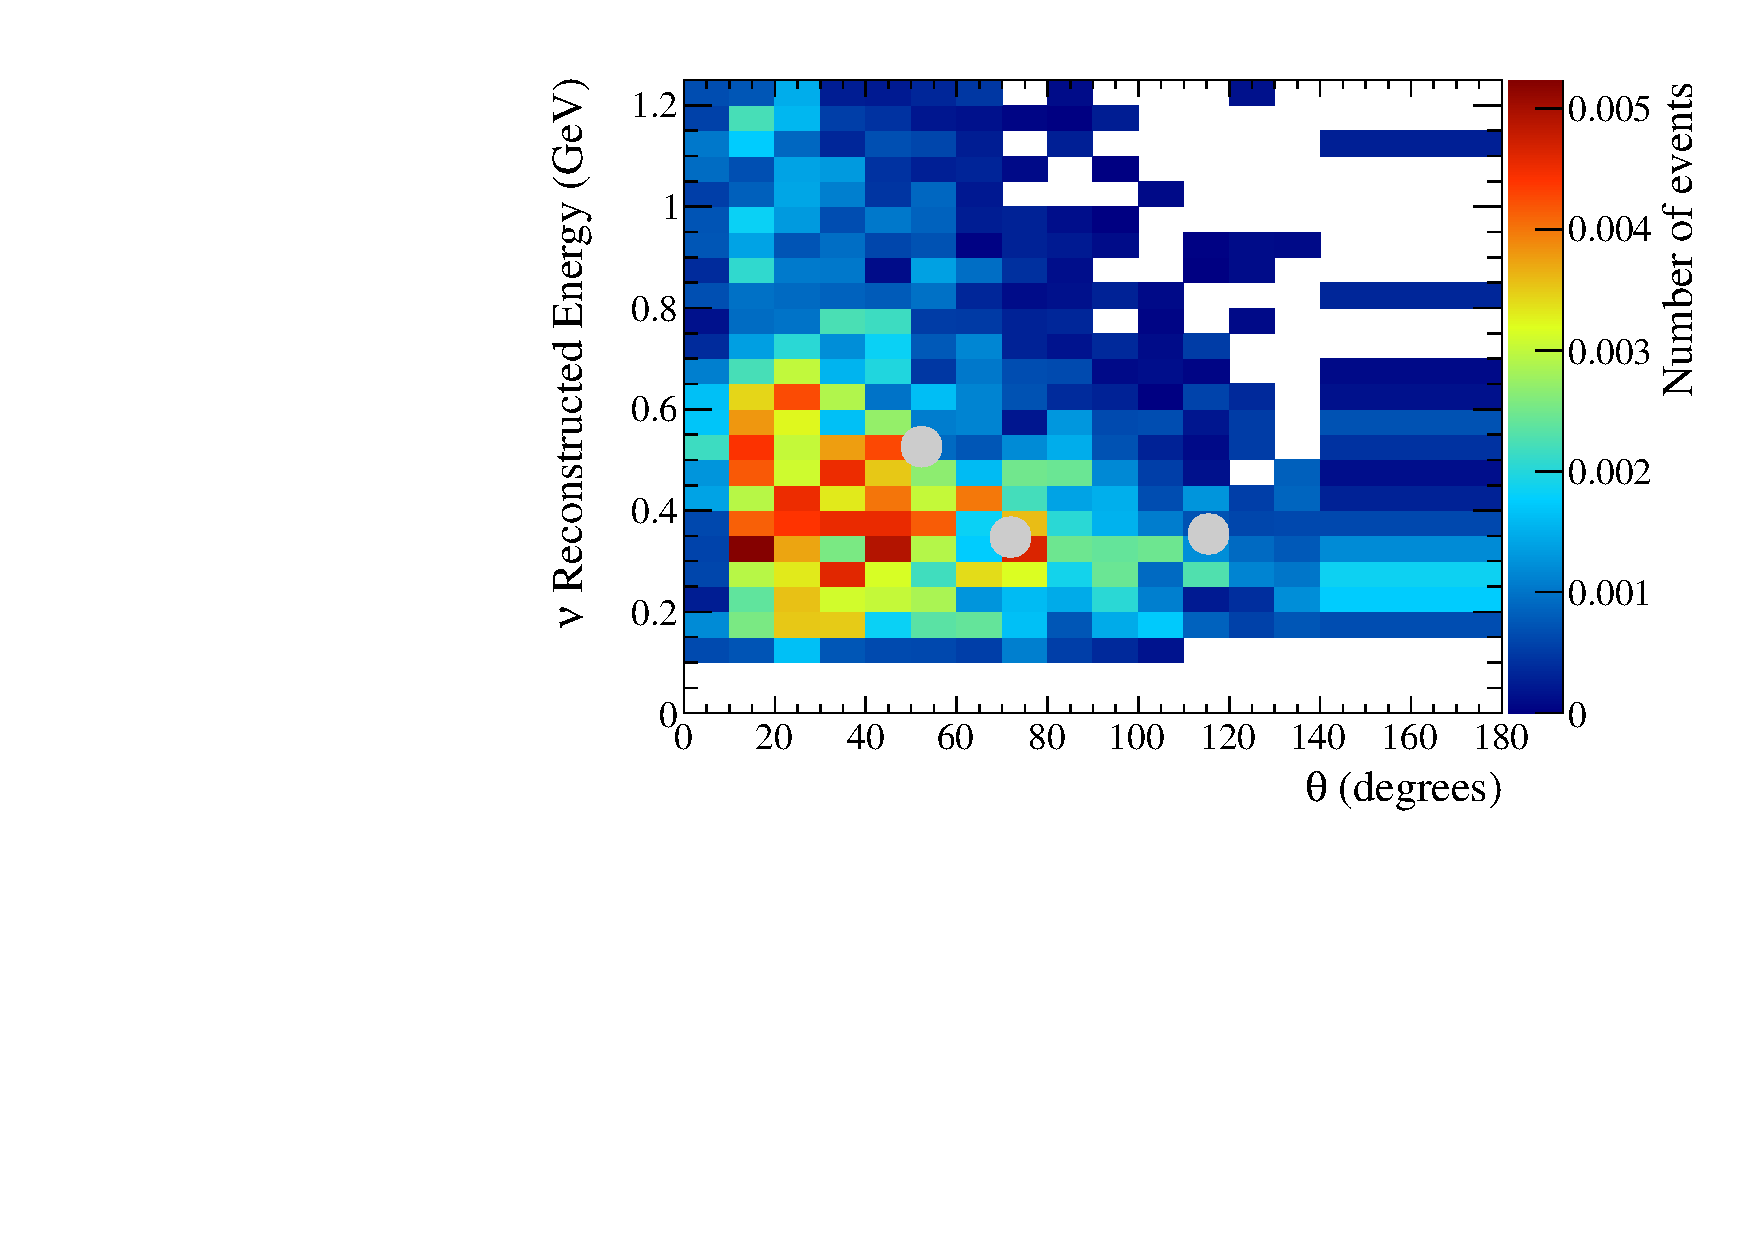
\includegraphics[width=0.9\textwidth]{./joint_plots/data/data_mc_rhc1re_2d_NC.pdf}
\caption{Neutral current.}
\end{subfigure}
\begin{subfigure}[b]{0.49\textwidth}
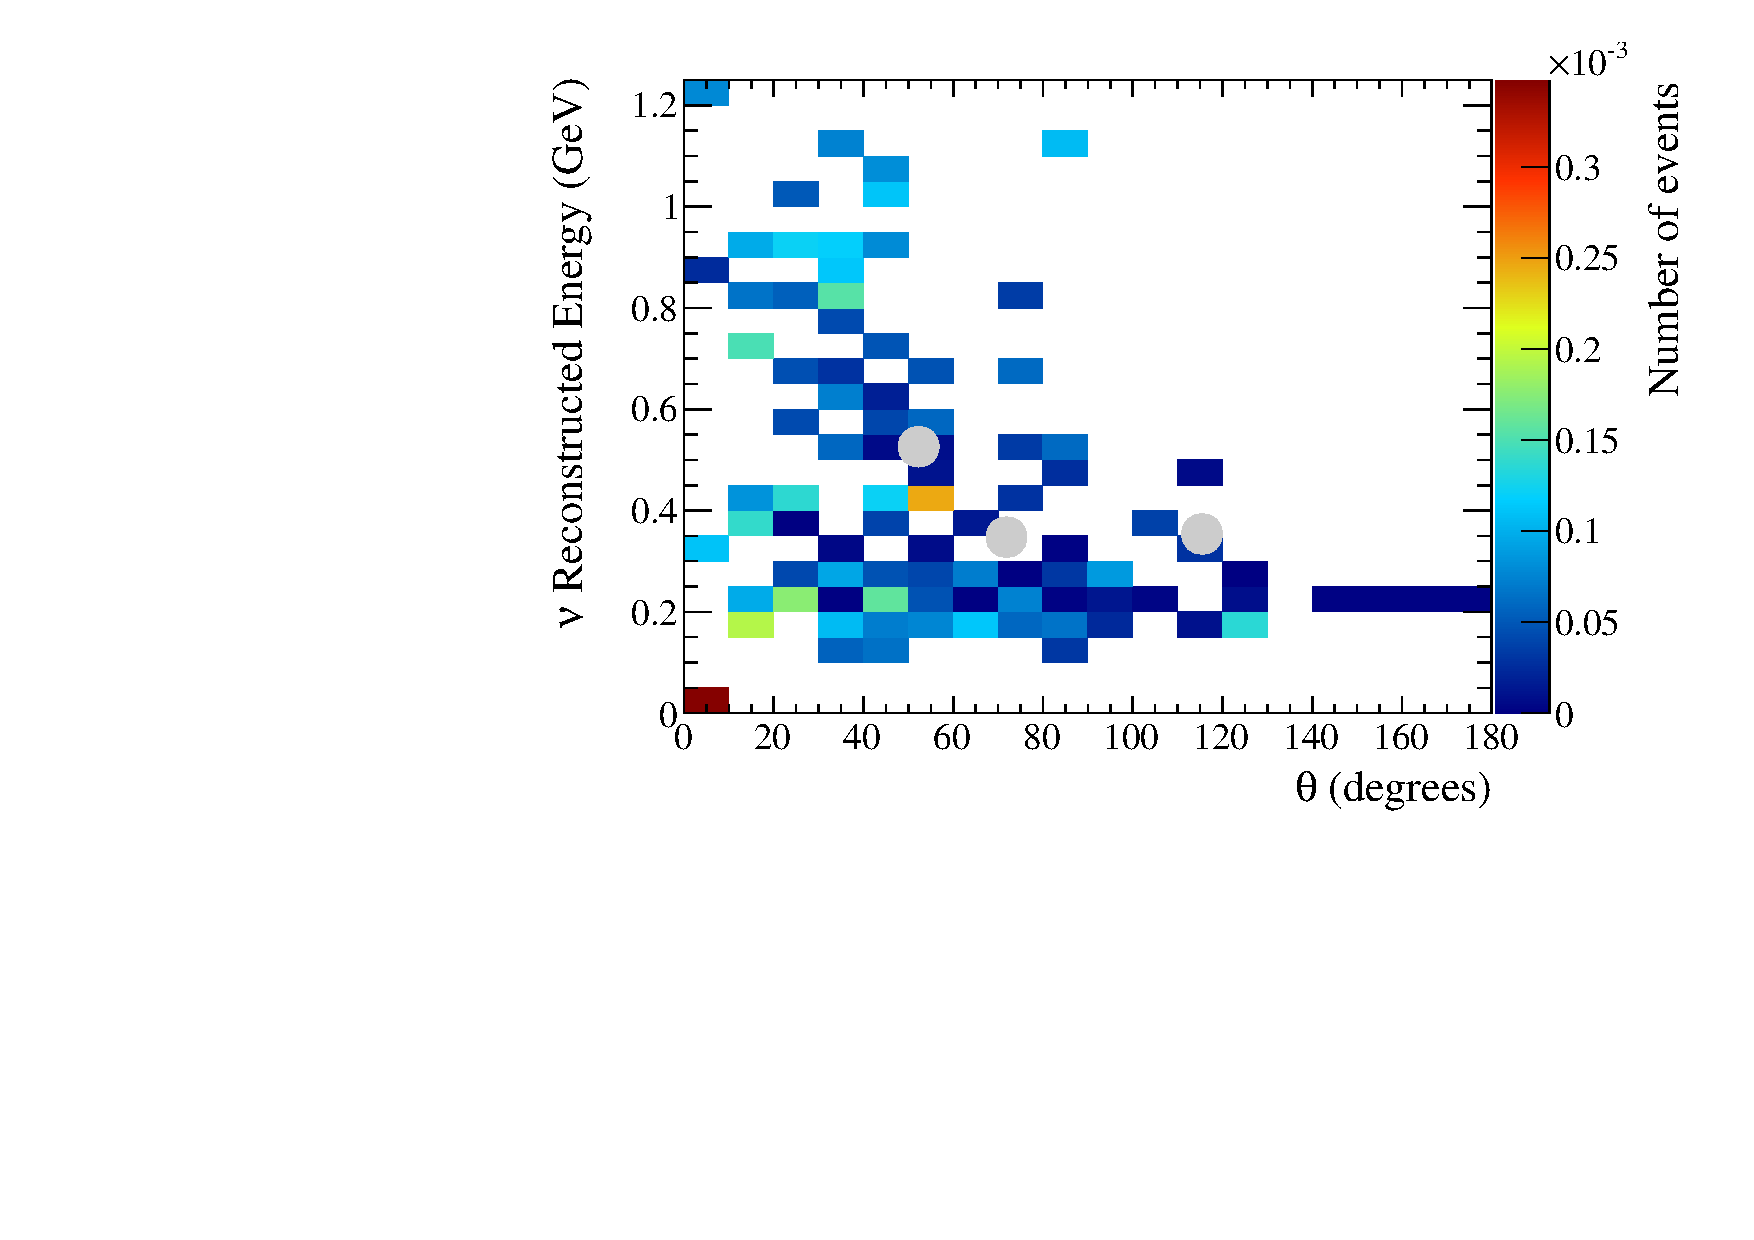
\includegraphics[width=0.9\textwidth]{./joint_plots/data/data_mc_rhc1re_2d_NumuBeam.pdf}
\caption{$\nu_{\mu}$ intrinsic beam.}
\end{subfigure}
\begin{subfigure}[b]{0.49\textwidth}
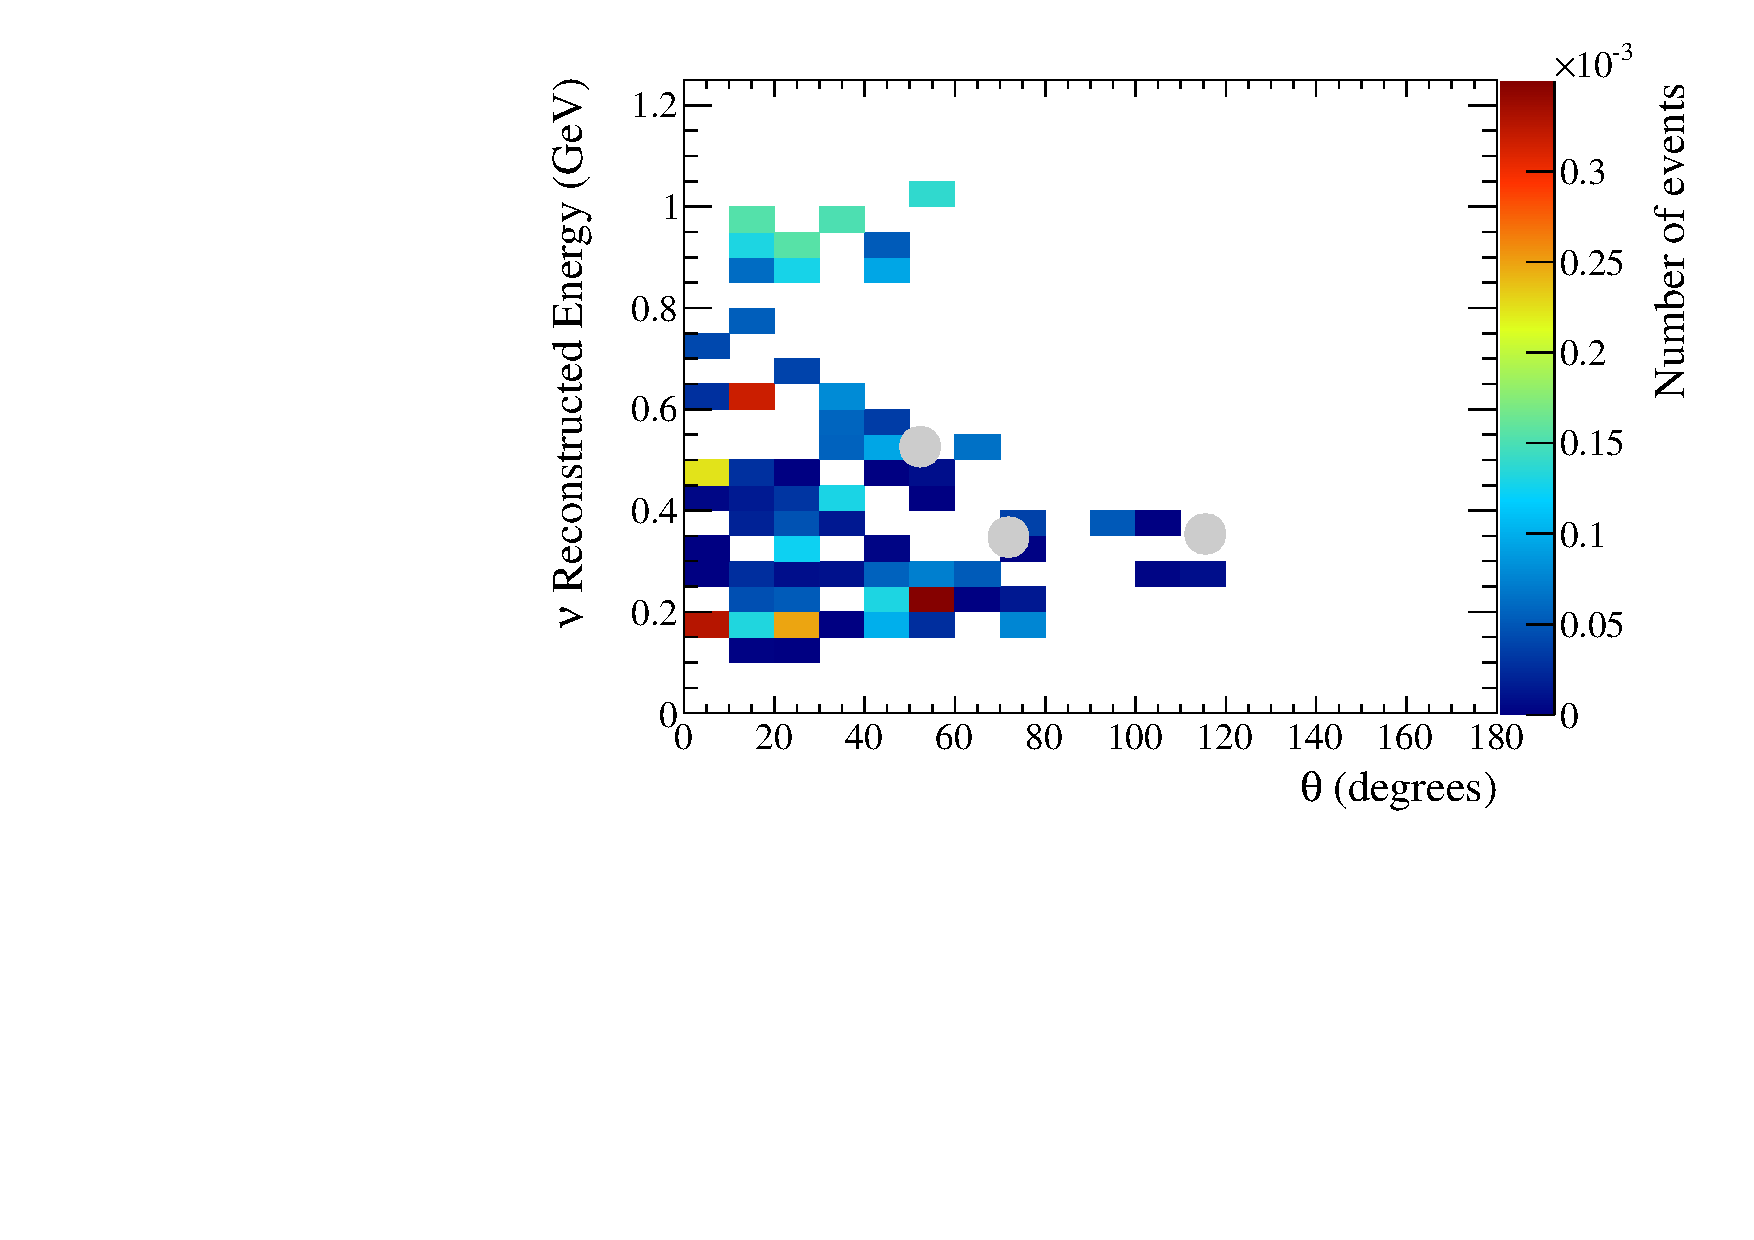
\includegraphics[width=0.9\textwidth]{./joint_plots/data/data_mc_rhc1re_2d_NumuBarBeam.pdf}
\caption{$\bar{\nu}_{\mu}$ intrinsic beam.}
\end{subfigure}
\caption {
Predicted and observed (grey dots) spectra of electron-like events
as a function of the reconstructed neutrino energy and
the angle between the outgoing lepton and the neutrino direction.
The distributions correspond to the collected statistics in the full Run 1-6 data set.
%for an exposure 
%of $6.914 \times 10^{20}$ POT in neutrino  mode.
%and
%of $4.011 \times 10^{20}$ POT in antineutrino mode.
From top left to bottom right the following components are shown:
%total,
$\nu_{\mu} \rightarrow \nu_e$,
$\bar{\nu}_{\mu} \rightarrow \bar{\nu}_e$,
$\nu_e + \bar{\nu}_e$ intrinsic beam,
NC,
$\nu_{\mu}$ intrinsic beam
and
$\bar{\nu}_{\mu}$ intrinsic beam.
The spectra were generated with the systematic parameters measured with the ND280 data 
shown in \cref{tab:banff_uncertainties_flux_fhc},~\ref{tab:banff_uncertainties_flux_rhc},~\ref{tab:banff_uncertainties_xsec},
the nominal Super-K systematic parameters shown in \cref{tab:banff_uncertainties_skdetfsi}
and the oscillation parameters corresponding to the Asimov data set A shown in \cref{tab:osc_params_joint_asimov}.
}
\label{fig:joint_ereco_vs_theta_rhc1re_data}
\end{figure*}


\clearpage




%...........................................................
%
% Predicted number of events
%
%...........................................................

\section{Effect of systematic uncertainties}
\label{app:systematics}

In \cref{tab:apply_syst_to_template_mulike_fhc},
\ref{tab:apply_syst_to_template_elike_fhc},
\ref{tab:apply_syst_to_template_mulike_rhc} and
\ref{tab:apply_syst_to_template_elike_rhc}
it is shown which systematic parameter is applied to which reaction and flavour modes 
for all the Super-K samples.
 
\afterpage{%\documentclass[10pt]{article}
%\usepackage[utf8]{inputenc}
%\usepackage{amsmath}
%\usepackage{amsfonts}
%\usepackage{amssymb}
%\usepackage{fullpage}
%\usepackage{rotate}  
%\usepackage{rotating}
%\usepackage[paperwidth=300mm,paperheight=450mm]{geometry}

%\newcommand{\ck}{$\checkmark$}
%\begin{document}

{
\setlength{\tabcolsep}{2pt}
\renewcommand{\arraystretch}{1.5}
\begin{landscape}
\begin{footnotesize}

\begin{longtable} { | c ||c | c | c | c | c | c | c | c | c | c | c | c | c | c | c | c | c | c | c | c | c | c | c | c | c | c | c | c | c | c | c | c | c | c | c | c | c | c | c | c | c | c | c | c | c | c | c | c | c | c |  | }
\hline
 & \begin{sideways} $\nu_\mu$ CCQE \end{sideways} 
 & \begin{sideways} $\nu_\mu$ CC 1$\pi$ \end{sideways} 
 & \begin{sideways} $\nu_\mu$ CC coherent \end{sideways} 
 & \begin{sideways} $\nu_\mu$ CC 2p-2h \end{sideways} 
 & \begin{sideways} $\nu_\mu$ CC other \end{sideways} 
 & \begin{sideways} $\nu_\mu$/$\nu_\tau$ NC 1$\pi^{+/-}$ \end{sideways} 
 & \begin{sideways} $\nu_\mu$/$\nu_\tau$ NC 1$\pi^0$ \end{sideways} 
 & \begin{sideways} $\nu_\mu$/$\nu_\tau$ NC coherent \end{sideways} 
 & \begin{sideways} $\nu_\mu$/$\nu_\tau$ NC other \end{sideways} 
 & \begin{sideways} $\nu_e$ NC 1$\gamma$ \end{sideways} 
 & \begin{sideways} $\bar{\nu}_\mu$ CCQE \end{sideways} 
 & \begin{sideways} $\bar{\nu}_\mu$ CC 1$\pi$ \end{sideways} 
 & \begin{sideways} $\bar{\nu}_\mu$ CC coherent \end{sideways} 
 & \begin{sideways} $\bar{\nu}_\mu$ CC 2p-2h \end{sideways} 
 & \begin{sideways} $\bar{\nu}_\mu$ CC other \end{sideways} 
 & \begin{sideways} $\bar{\nu}_\mu$/$\bar{\nu}_\tau$ NC 1$\pi^{+/-}$ \end{sideways} 
 & \begin{sideways} $\bar{\nu}_\mu$/$\bar{\nu}_\tau$ NC 1$\pi^0$ \end{sideways} 
 & \begin{sideways} $\bar{\nu}_\mu$/$\bar{\nu}_\tau$ NC coherent \end{sideways} 
 & \begin{sideways} $\bar{\nu}_\mu$/$\bar{\nu}_\tau$ NC other \end{sideways} 
 & \begin{sideways} $\nu_\mu$ NC 1$\gamma$ \end{sideways} 
 & \begin{sideways} $\nu_e$ CCQE \end{sideways} 
 & \begin{sideways} $\nu_e$ CC 1$\pi$ \end{sideways} 
 & \begin{sideways} $\nu_e$ CC coherent \end{sideways} 
 & \begin{sideways} $\nu_e$ CC 2p-2h \end{sideways} 
 & \begin{sideways} $\nu_e$ CC other \end{sideways} 
 & \begin{sideways} $\nu_e$ NC 1$\pi^{+/-}$ \end{sideways} 
 & \begin{sideways} $\nu_e$ NC 1$\pi^0$ \end{sideways} 
 & \begin{sideways} $\nu_e$ NC coherent \end{sideways} 
 & \begin{sideways} $\nu_e$ NC other \end{sideways} 
 & \begin{sideways} $\bar{\nu}_\mu$ NC 1$\gamma$ \end{sideways} 
 & \begin{sideways} Osc. $\nu_e$ CCQE \end{sideways} 
 & \begin{sideways} Osc. $\nu_e$ CC 1$\pi$ \end{sideways} 
 & \begin{sideways} Osc. $\nu_e$ CC coherent \end{sideways} 
 & \begin{sideways} Osc. $\nu_e$ CC 2p-2h \end{sideways} 
 & \begin{sideways} Osc. $\nu_e$ CC other \end{sideways} 
 & \begin{sideways} $\bar{\nu}_e$ CCQE \end{sideways} 
 & \begin{sideways} $\bar{\nu}_e$ CC 1$\pi$ \end{sideways} 
 & \begin{sideways} $\bar{\nu}_e$ CC coherent \end{sideways} 
 & \begin{sideways} $\bar{\nu}_e$ CC 2p-2h \end{sideways} 
 & \begin{sideways} $\bar{\nu}_e$ CC other \end{sideways} 
 & \begin{sideways} $\bar{\nu}_e$ NC 1$\pi^{+/-}$ \end{sideways} 
 & \begin{sideways} $\bar{\nu}_e$ NC 1$\pi^0$ \end{sideways} 
 & \begin{sideways} $\bar{\nu}_e$ NC coherent \end{sideways} 
 & \begin{sideways} $\bar{\nu}_e$ NC other \end{sideways} 
 & \begin{sideways} $\bar{\nu}_e$ NC 1$\gamma$ \end{sideways} 
 & \begin{sideways} Osc. $\bar{\nu}_e$ CCQE \end{sideways} 
 & \begin{sideways} Osc. $\bar{\nu}_e$ CC 1$\pi$ \end{sideways} 
 & \begin{sideways} Osc. $\bar{\nu}_e$ CC coherent \end{sideways} 
 & \begin{sideways} Osc. $\bar{\nu}_e$ CC 2p-2h \end{sideways} 
 & \begin{sideways} Osc. $\bar{\nu}_e$ CC other \end{sideways} 
\\ \hline 
%$\sin^2(\theta_{12})$         & \ck& \ck& \ck& \ck& \ck&    &    &    &    &    & \ck& \ck& \ck& \ck& \ck&    &    &    &    &    & \ck& \ck& \ck& \ck& \ck&    &    &    &    &    & \ck& \ck& \ck& \ck& \ck& \ck& \ck& \ck& \ck& \ck&    &    &    &    &    & \ck& \ck& \ck& \ck& \ck \\ \hline 
%$\sin^2(\theta_{13})$         & \ck& \ck& \ck& \ck& \ck&    &    &    &    &    & \ck& \ck& \ck& \ck& \ck&    &    &    &    &    & \ck& \ck& \ck& \ck& \ck&    &    &    &    &    & \ck& \ck& \ck& \ck& \ck& \ck& \ck& \ck& \ck& \ck&    &    &    &    &    & \ck& \ck& \ck& \ck& \ck \\ \hline 
%$\Delta m^2_{21}$             & \ck& \ck& \ck& \ck& \ck&    &    &    &    &    & \ck& \ck& \ck& \ck& \ck&    &    &    &    &    & \ck& \ck& \ck& \ck& \ck&    &    &    &    &    & \ck& \ck& \ck& \ck& \ck& \ck& \ck& \ck& \ck& \ck&    &    &    &    &    & \ck& \ck& \ck& \ck& \ck \\ \hline 
%$\delta_{CP}$                 & \ck& \ck& \ck& \ck& \ck&    &    &    &    &    & \ck& \ck& \ck& \ck& \ck&    &    &    &    &    & \ck& \ck& \ck& \ck& \ck&    &    &    &    &    & \ck& \ck& \ck& \ck& \ck& \ck& \ck& \ck& \ck& \ck&    &    &    &    &    & \ck& \ck& \ck& \ck& \ck \\ \hline 
$f_{E; r}^{SK}$               & \ck& \ck& \ck& \ck& \ck& \ck& \ck& \ck& \ck& \ck& \ck& \ck& \ck& \ck& \ck& \ck& \ck& \ck& \ck& \ck& \ck& \ck& \ck& \ck& \ck& \ck& \ck& \ck& \ck& \ck& \ck& \ck& \ck& \ck& \ck& \ck& \ck& \ck& \ck& \ck& \ck& \ck& \ck& \ck& \ck& \ck& \ck& \ck& \ck& \ck \\ \hline 
$f_{0; t, r}^{SK+FSI}$        & \ck&    &    & \ck&    &    &    &    &    &    & \ck&    &    & \ck&    &    &    &    &    &    &    &    &    &    &    &    &    &    &    &    &    &    &    &    &    &    &    &    &    &    &    &    &    &    &    &    &    &    &    &     \\ \hline 
$f_{1; t, r}^{SK+FSI}$        & \ck&    &    & \ck&    &    &    &    &    &    & \ck&    &    & \ck&    &    &    &    &    &    &    &    &    &    &    &    &    &    &    &    &    &    &    &    &    &    &    &    &    &    &    &    &    &    &    &    &    &    &    &     \\ \hline 
$f_{2; t, r}^{SK+FSI}$        & \ck&    &    & \ck&    &    &    &    &    &    & \ck&    &    & \ck&    &    &    &    &    &    &    &    &    &    &    &    &    &    &    &    &    &    &    &    &    &    &    &    &    &    &    &    &    &    &    &    &    &    &    &     \\ \hline 
$f_{3; t, r}^{SK+FSI}$        &    & \ck& \ck&    & \ck&    &    &    &    &    &    & \ck& \ck&    & \ck&    &    &    &    &    &    &    &    &    &    &    &    &    &    &    &    &    &    &    &    &    &    &    &    &    &    &    &    &    &    &    &    &    &    &     \\ \hline 
$f_{4; t, r}^{SK+FSI}$        &    &    &    &    &    &    &    &    &    &    &    &    &    &    &    &    &    &    &    &    & \ck& \ck& \ck& \ck& \ck&    &    &    &    &    & \ck& \ck& \ck& \ck& \ck& \ck& \ck& \ck& \ck& \ck&    &    &    &    &    & \ck& \ck& \ck& \ck& \ck \\ \hline 
$f_{5; t, r}^{SK+FSI}$        &    &    &    &    &    & \ck& \ck& \ck& \ck& \ck&    &    &    &    &    & \ck& \ck& \ck& \ck& \ck&    &    &    &    &    & \ck& \ck& \ck& \ck& \ck&    &    &    &    &    &    &    &    &    &    & \ck& \ck& \ck& \ck& \ck&    &    &    &    &     \\ \hline 
$f_{0; t, r}^{banff}$         & \ck& \ck& \ck& \ck& \ck& \ck& \ck& \ck& \ck& \ck&    &    &    &    &    &    &    &    &    &    &    &    &    &    &    &    &    &    &    &    & \ck& \ck& \ck& \ck& \ck&    &    &    &    &    &    &    &    &    &    &    &    &    &    &     \\ \hline 
$f_{1; t, r}^{banff}$         & \ck& \ck& \ck& \ck& \ck& \ck& \ck& \ck& \ck& \ck&    &    &    &    &    &    &    &    &    &    &    &    &    &    &    &    &    &    &    &    & \ck& \ck& \ck& \ck& \ck&    &    &    &    &    &    &    &    &    &    &    &    &    &    &     \\ \hline 
$f_{2; t, r}^{banff}$         & \ck& \ck& \ck& \ck& \ck& \ck& \ck& \ck& \ck& \ck&    &    &    &    &    &    &    &    &    &    &    &    &    &    &    &    &    &    &    &    & \ck& \ck& \ck& \ck& \ck&    &    &    &    &    &    &    &    &    &    &    &    &    &    &     \\ \hline 
$f_{3; t, r}^{banff}$         & \ck& \ck& \ck& \ck& \ck& \ck& \ck& \ck& \ck& \ck&    &    &    &    &    &    &    &    &    &    &    &    &    &    &    &    &    &    &    &    & \ck& \ck& \ck& \ck& \ck&    &    &    &    &    &    &    &    &    &    &    &    &    &    &     \\ \hline 
$f_{4; t, r}^{banff}$         & \ck& \ck& \ck& \ck& \ck& \ck& \ck& \ck& \ck& \ck&    &    &    &    &    &    &    &    &    &    &    &    &    &    &    &    &    &    &    &    & \ck& \ck& \ck& \ck& \ck&    &    &    &    &    &    &    &    &    &    &    &    &    &    &     \\ \hline 
$f_{5; t, r}^{banff}$         & \ck& \ck& \ck& \ck& \ck& \ck& \ck& \ck& \ck& \ck&    &    &    &    &    &    &    &    &    &    &    &    &    &    &    &    &    &    &    &    & \ck& \ck& \ck& \ck& \ck&    &    &    &    &    &    &    &    &    &    &    &    &    &    &     \\ \hline 
$f_{6; t, r}^{banff}$         & \ck& \ck& \ck& \ck& \ck& \ck& \ck& \ck& \ck& \ck&    &    &    &    &    &    &    &    &    &    &    &    &    &    &    &    &    &    &    &    & \ck& \ck& \ck& \ck& \ck&    &    &    &    &    &    &    &    &    &    &    &    &    &    &     \\ \hline 
$f_{7; t, r}^{banff}$         & \ck& \ck& \ck& \ck& \ck& \ck& \ck& \ck& \ck& \ck&    &    &    &    &    &    &    &    &    &    &    &    &    &    &    &    &    &    &    &    & \ck& \ck& \ck& \ck& \ck&    &    &    &    &    &    &    &    &    &    &    &    &    &    &     \\ \hline 
$f_{8; t, r}^{banff}$         & \ck& \ck& \ck& \ck& \ck& \ck& \ck& \ck& \ck& \ck&    &    &    &    &    &    &    &    &    &    &    &    &    &    &    &    &    &    &    &    & \ck& \ck& \ck& \ck& \ck&    &    &    &    &    &    &    &    &    &    &    &    &    &    &     \\ \hline 
$f_{9; t, r}^{banff}$         & \ck& \ck& \ck& \ck& \ck& \ck& \ck& \ck& \ck& \ck&    &    &    &    &    &    &    &    &    &    &    &    &    &    &    &    &    &    &    &    & \ck& \ck& \ck& \ck& \ck&    &    &    &    &    &    &    &    &    &    &    &    &    &    &     \\ \hline 
$f_{10; t, r}^{banff}$        & \ck& \ck& \ck& \ck& \ck& \ck& \ck& \ck& \ck& \ck&    &    &    &    &    &    &    &    &    &    &    &    &    &    &    &    &    &    &    &    & \ck& \ck& \ck& \ck& \ck&    &    &    &    &    &    &    &    &    &    &    &    &    &    &     \\ \hline 
$f_{11; t, r}^{banff}$        &    &    &    &    &    &    &    &    &    &    & \ck& \ck& \ck& \ck& \ck& \ck& \ck& \ck& \ck& \ck&    &    &    &    &    &    &    &    &    &    &    &    &    &    &    &    &    &    &    &    &    &    &    &    &    & \ck& \ck& \ck& \ck& \ck \\ \hline 
$f_{12; t, r}^{banff}$        &    &    &    &    &    &    &    &    &    &    & \ck& \ck& \ck& \ck& \ck& \ck& \ck& \ck& \ck& \ck&    &    &    &    &    &    &    &    &    &    &    &    &    &    &    &    &    &    &    &    &    &    &    &    &    & \ck& \ck& \ck& \ck& \ck \\ \hline 
$f_{13; t, r}^{banff}$        &    &    &    &    &    &    &    &    &    &    & \ck& \ck& \ck& \ck& \ck& \ck& \ck& \ck& \ck& \ck&    &    &    &    &    &    &    &    &    &    &    &    &    &    &    &    &    &    &    &    &    &    &    &    &    & \ck& \ck& \ck& \ck& \ck \\ \hline 
$f_{14; t, r}^{banff}$        &    &    &    &    &    &    &    &    &    &    & \ck& \ck& \ck& \ck& \ck& \ck& \ck& \ck& \ck& \ck&    &    &    &    &    &    &    &    &    &    &    &    &    &    &    &    &    &    &    &    &    &    &    &    &    & \ck& \ck& \ck& \ck& \ck \\ \hline 
$f_{15; t, r}^{banff}$        &    &    &    &    &    &    &    &    &    &    & \ck& \ck& \ck& \ck& \ck& \ck& \ck& \ck& \ck& \ck&    &    &    &    &    &    &    &    &    &    &    &    &    &    &    &    &    &    &    &    &    &    &    &    &    & \ck& \ck& \ck& \ck& \ck \\ \hline 
$f_{16; t, r}^{banff}$        &    &    &    &    &    &    &    &    &    &    &    &    &    &    &    &    &    &    &    &    & \ck& \ck& \ck& \ck& \ck& \ck& \ck& \ck& \ck& \ck&    &    &    &    &    &    &    &    &    &    &    &    &    &    &    &    &    &    &    &     \\ \hline 
$f_{17; t, r}^{banff}$        &    &    &    &    &    &    &    &    &    &    &    &    &    &    &    &    &    &    &    &    & \ck& \ck& \ck& \ck& \ck& \ck& \ck& \ck& \ck& \ck&    &    &    &    &    &    &    &    &    &    &    &    &    &    &    &    &    &    &    &     \\ \hline 
$f_{18; t, r}^{banff}$        &    &    &    &    &    &    &    &    &    &    &    &    &    &    &    &    &    &    &    &    & \ck& \ck& \ck& \ck& \ck& \ck& \ck& \ck& \ck& \ck&    &    &    &    &    &    &    &    &    &    &    &    &    &    &    &    &    &    &    &     \\ \hline 
$f_{19; t, r}^{banff}$        &    &    &    &    &    &    &    &    &    &    &    &    &    &    &    &    &    &    &    &    & \ck& \ck& \ck& \ck& \ck& \ck& \ck& \ck& \ck& \ck&    &    &    &    &    &    &    &    &    &    &    &    &    &    &    &    &    &    &    &     \\ \hline 
$f_{20; t, r}^{banff}$        &    &    &    &    &    &    &    &    &    &    &    &    &    &    &    &    &    &    &    &    & \ck& \ck& \ck& \ck& \ck& \ck& \ck& \ck& \ck& \ck&    &    &    &    &    &    &    &    &    &    &    &    &    &    &    &    &    &    &    &     \\ \hline 
$f_{21; t, r}^{banff}$        &    &    &    &    &    &    &    &    &    &    &    &    &    &    &    &    &    &    &    &    & \ck& \ck& \ck& \ck& \ck& \ck& \ck& \ck& \ck& \ck&    &    &    &    &    &    &    &    &    &    &    &    &    &    &    &    &    &    &    &     \\ \hline 
$f_{22; t, r}^{banff}$        &    &    &    &    &    &    &    &    &    &    &    &    &    &    &    &    &    &    &    &    & \ck& \ck& \ck& \ck& \ck& \ck& \ck& \ck& \ck& \ck&    &    &    &    &    &    &    &    &    &    &    &    &    &    &    &    &    &    &    &     \\ \hline 
$f_{23; t, r}^{banff}$        &    &    &    &    &    &    &    &    &    &    &    &    &    &    &    &    &    &    &    &    &    &    &    &    &    &    &    &    &    &    &    &    &    &    &    & \ck& \ck& \ck& \ck& \ck& \ck& \ck& \ck& \ck& \ck&    &    &    &    &     \\ \hline 
$f_{24; t, r}^{banff}$        &    &    &    &    &    &    &    &    &    &    &    &    &    &    &    &    &    &    &    &    &    &    &    &    &    &    &    &    &    &    &    &    &    &    &    & \ck& \ck& \ck& \ck& \ck& \ck& \ck& \ck& \ck& \ck&    &    &    &    &     \\ \hline 
$f_{M_A^{QE}}^{banff}$        & \ck&    &    &    &    &    &    &    &    &    & \ck&    &    &    &    &    &    &    &    &    & \ck&    &    &    &    &    &    &    &    &    & \ck&    &    &    &    & \ck&    &    &    &    &    &    &    &    &    & \ck&    &    &    &     \\ \hline 
$f_{M_A^{RES}}^{banff}$       &    & \ck&    &    &    & \ck& \ck&    &    &    &    & \ck&    &    &    & \ck& \ck&    &    &    &    & \ck&    &    &    & \ck& \ck&    &    &    &    & \ck&    &    &    &    & \ck&    &    &    & \ck& \ck&    &    &    &    & \ck&    &    &     \\ \hline 
$f_{Norm_{2p-2h}}^{banff}$      &    &    &    & \ck&    &    &    &    &    &    &    &    &    & \ck&    &    &    &    &    &    &    &    &    & \ck&    &    &    &    &    &    &    &    &    & \ck&    &    &    &    & \ck&    &    &    &    &    &    &    &    &    & \ck&     \\ \hline 
$f_{C^{A}_{5}}^{banff}$       &    & \ck&    &    &    & \ck& \ck&    &    &    &    & \ck&    &    &    & \ck& \ck&    &    &    &    & \ck&    &    &    & \ck& \ck&    &    &    &    & \ck&    &    &    &    & \ck&    &    &    & \ck& \ck&    &    &    &    & \ck&    &    &     \\ \hline 
$f_{Bg_{RES}}^{banff}$        &    & \ck&    &    &    & \ck& \ck&    &    &    &    & \ck&    &    &    & \ck& \ck&    &    &    &    & \ck&    &    &    & \ck& \ck&    &    &    &    & \ck&    &    &    &    & \ck&    &    &    & \ck& \ck&    &    &    &    & \ck&    &    &     \\ \hline 
$f_{p_{f}}^{banff}$           & \ck&    &    &    &    &    &    &    &    &    & \ck&    &    &    &    &    &    &    &    &    & \ck&    &    &    &    &    &    &    &    &    & \ck&    &    &    &    & \ck&    &    &    &    &    &    &    &    &    & \ck&    &    &    &     \\ \hline 
$f_{Shape_{CCoth}}^{banff}$   &    &    &    &    & \ck&    &    &    &    &    &    &    &    &    & \ck&    &    &    &    &    &    &    &    &    & \ck&    &    &    &    &    &    &    &    &    & \ck&    &    &    &    & \ck&    &    &    &    &    &    &    &    &    & \ck \\ \hline 
$f_{E_{B}}^{banff}$           & \ck&    &    &    &    &    &    &    &    &    & \ck&    &    &    &    &    &    &    &    &    & \ck&    &    &    &    &    &    &    &    &    & \ck&    &    &    &    & \ck&    &    &    &    &    &    &    &    &    & \ck&    &    &    &     \\ \hline 
$f_{Norm_{CCcoh}}^{banff}$    &    &    & \ck&    &    &    &    &    &    &    &    &    & \ck&    &    &    &    &    &    &    &    &    & \ck&    &    &    &    &    &    &    &    &    & \ck&    &    &    &    & \ck&    &    &    &    &    &    &    &    &    & \ck&    &     \\ \hline 
$f_{Norm_{NCcoh}}^{banff}$    &    &    &    &    &    &    &    & \ck&    &    &    &    &    &    &    &    &    & \ck&    &    &    &    &    &    &    &    &    & \ck&    &    &    &    &    &    &    &    &    &    &    &    &    &    & \ck&    &    &    &    &    &    &     \\ \hline 
$f_{Norm_{NCother}}^{banff}$  &    &    &    &    &    &    &    &    & \ck&    &    &    &    &    &    &    &    &    & \ck&    &    &    &    &    &    &    &    &    & \ck&    &    &    &    &    &    &    &    &    &    &    &    &    &    & \ck&    &    &    &    &    &     \\ \hline 
$f_{Norm_{\nu_e \rightarrow \nu_\mu}}^{banff}$&    &    &    &    &    &    &    &    &    &    &    &    &    &    &    &    &    &    &    &    & \ck& \ck& \ck& \ck& \ck&    &    &    &    &    & \ck& \ck& \ck& \ck& \ck&    &    &    &    &    &    &    &    &    &    &    &    &    &    &     \\ \hline 
$f_{Norm_{NC1\gamma}}^{banff}$&    &    &    &    &    &    &    &    &    & \ck&    &    &    &    &    &    &    &    &    & \ck&    &    &    &    &    &    &    &    &    & \ck&    &    &    &    &    &    &    &    &    &    &    &    &    &    & \ck&    &    &    &    &     \\ \hline 
$f_{Norm_{\bar{\nu}_e \rightarrow \bar{\nu}_\mu}}^{banff}$&    &    &    &    &    &    &    &    &    &    &    &    &    &    &    &    &    &    &    &    &    &    &    &    &    &    &    &    &    &    &    &    &    &    &    & \ck& \ck& \ck& \ck& \ck&    &    &    &    &    & \ck& \ck& \ck& \ck& \ck \\ \hline 
$f_{Norm_{2p-2h-Bar}}^{banff}$   &    &    &    &    &    &    &    &    &    &    &    &    &    & \ck&    &    &    &    &    &    &    &    &    &    &    &    &    &    &    &    &    &    &    &    &    &    &    &    & \ck&    &    &    &    &    &    &    &    &    & \ck&     \\ \hline 

\caption{
Each row of this table represents one of the \NSyst systematic parameters (oscillation excluded) considered in this analysis and each column represents 
 one of the \NMCTemplate{} MC templates used to construct the single $\mu$-like ring reconstructed energy spectrum p.d.f. in neutrino mode. 
 A \ck symbol denotes that the given MC template is modified when the given systematic parameter is tweaked.
 Only the systematic parameters that affect this sample are shown.
     % \huge{TO UPDATE} % caption is already ok
}
\label{tab:apply_syst_to_template_mulike_fhc}
\end{longtable}
\end{footnotesize}
\end{landscape}
}
}
\afterpage{%\documentclass[10pt]{article}
%\usepackage[utf8]{inputenc}
%\usepackage{amsmath}
%\usepackage{amsfonts}
%\usepackage{amssymb}
%\usepackage{fullpage}
%\usepackage{rotate}  
%\usepackage{rotating}
%\usepackage[paperwidth=300mm,paperheight=450mm]{geometry}

%\newcommand{\ck}{$\checkmark$}
%\begin{document}

{
\setlength{\tabcolsep}{2pt}
\renewcommand{\arraystretch}{1.5}
\begin{landscape}
\begin{footnotesize}

\begin{longtable} { | c ||c | c | c | c | c | c | c | c | c | c | c | c | c | c | c | c | c | c | c | c | c | c | c | c | c | c | c | c | c | c | c | c | c | c | c | c | c | c | c | c | c | c | c | c | c | c | c | c | c | c |  | }
\hline
 & \begin{sideways} $\nu_\mu$ CCQE \end{sideways} 
 & \begin{sideways} $\nu_\mu$ CC 1$\pi$ \end{sideways} 
 & \begin{sideways} $\nu_\mu$ CC coherent \end{sideways} 
 & \begin{sideways} $\nu_\mu$ CC 2p-2h \end{sideways} 
 & \begin{sideways} $\nu_\mu$ CC other \end{sideways} 
 & \begin{sideways} $\nu_\mu$/$\nu_\tau$ NC 1$\pi^{+/-}$ \end{sideways} 
 & \begin{sideways} $\nu_\mu$/$\nu_\tau$ NC 1$\pi^0$ \end{sideways} 
 & \begin{sideways} $\nu_\mu$/$\nu_\tau$ NC coherent \end{sideways} 
 & \begin{sideways} $\nu_\mu$/$\nu_\tau$ NC other \end{sideways} 
 & \begin{sideways} $\nu_e$ NC 1$\gamma$ \end{sideways} 
 & \begin{sideways} $\bar{\nu}_\mu$ CCQE \end{sideways} 
 & \begin{sideways} $\bar{\nu}_\mu$ CC 1$\pi$ \end{sideways} 
 & \begin{sideways} $\bar{\nu}_\mu$ CC coherent \end{sideways} 
 & \begin{sideways} $\bar{\nu}_\mu$ CC 2p-2h \end{sideways} 
 & \begin{sideways} $\bar{\nu}_\mu$ CC other \end{sideways} 
 & \begin{sideways} $\bar{\nu}_\mu$/$\bar{\nu}_\tau$ NC 1$\pi^{+/-}$ \end{sideways} 
 & \begin{sideways} $\bar{\nu}_\mu$/$\bar{\nu}_\tau$ NC 1$\pi^0$ \end{sideways} 
 & \begin{sideways} $\bar{\nu}_\mu$/$\bar{\nu}_\tau$ NC coherent \end{sideways} 
 & \begin{sideways} $\bar{\nu}_\mu$/$\bar{\nu}_\tau$ NC other \end{sideways} 
 & \begin{sideways} $\nu_\mu$ NC 1$\gamma$ \end{sideways} 
 & \begin{sideways} $\nu_e$ CCQE \end{sideways} 
 & \begin{sideways} $\nu_e$ CC 1$\pi$ \end{sideways} 
 & \begin{sideways} $\nu_e$ CC coherent \end{sideways} 
 & \begin{sideways} $\nu_e$ CC 2p-2h \end{sideways} 
 & \begin{sideways} $\nu_e$ CC other \end{sideways} 
 & \begin{sideways} $\nu_e$ NC 1$\pi^{+/-}$ \end{sideways} 
 & \begin{sideways} $\nu_e$ NC 1$\pi^0$ \end{sideways} 
 & \begin{sideways} $\nu_e$ NC coherent \end{sideways} 
 & \begin{sideways} $\nu_e$ NC other \end{sideways} 
 & \begin{sideways} $\bar{\nu}_\mu$ NC 1$\gamma$ \end{sideways} 
 & \begin{sideways} Osc. $\nu_e$ CCQE \end{sideways} 
 & \begin{sideways} Osc. $\nu_e$ CC 1$\pi$ \end{sideways} 
 & \begin{sideways} Osc. $\nu_e$ CC coherent \end{sideways} 
 & \begin{sideways} Osc. $\nu_e$ CC 2p-2h \end{sideways} 
 & \begin{sideways} Osc. $\nu_e$ CC other \end{sideways} 
 & \begin{sideways} $\bar{\nu}_e$ CCQE \end{sideways} 
 & \begin{sideways} $\bar{\nu}_e$ CC 1$\pi$ \end{sideways} 
 & \begin{sideways} $\bar{\nu}_e$ CC coherent \end{sideways} 
 & \begin{sideways} $\bar{\nu}_e$ CC 2p-2h \end{sideways} 
 & \begin{sideways} $\bar{\nu}_e$ CC other \end{sideways} 
 & \begin{sideways} $\bar{\nu}_e$ NC 1$\pi^{+/-}$ \end{sideways} 
 & \begin{sideways} $\bar{\nu}_e$ NC 1$\pi^0$ \end{sideways} 
 & \begin{sideways} $\bar{\nu}_e$ NC coherent \end{sideways} 
 & \begin{sideways} $\bar{\nu}_e$ NC other \end{sideways} 
 & \begin{sideways} $\bar{\nu}_e$ NC 1$\gamma$ \end{sideways} 
 & \begin{sideways} Osc. $\bar{\nu}_e$ CCQE \end{sideways} 
 & \begin{sideways} Osc. $\bar{\nu}_e$ CC 1$\pi$ \end{sideways} 
 & \begin{sideways} Osc. $\bar{\nu}_e$ CC coherent \end{sideways} 
 & \begin{sideways} Osc. $\bar{\nu}_e$ CC 2p-2h \end{sideways} 
 & \begin{sideways} Osc. $\bar{\nu}_e$ CC other \end{sideways} 
\\ \hline 
%$\sin^2(\theta_{12})$         & \ck& \ck& \ck& \ck& \ck&    &    &    &    &    & \ck& \ck& \ck& \ck& \ck&    &    &    &    &    & \ck& \ck& \ck& \ck& \ck&    &    &    &    &    & \ck& \ck& \ck& \ck& \ck& \ck& \ck& \ck& \ck& \ck&    &    &    &    &    & \ck& \ck& \ck& \ck& \ck \\ \hline 
%$\sin^2(\theta_{13})$         & \ck& \ck& \ck& \ck& \ck&    &    &    &    &    & \ck& \ck& \ck& \ck& \ck&    &    &    &    &    & \ck& \ck& \ck& \ck& \ck&    &    &    &    &    & \ck& \ck& \ck& \ck& \ck& \ck& \ck& \ck& \ck& \ck&    &    &    &    &    & \ck& \ck& \ck& \ck& \ck \\ \hline 
%$\Delta m^2_{21}$             & \ck& \ck& \ck& \ck& \ck&    &    &    &    &    & \ck& \ck& \ck& \ck& \ck&    &    &    &    &    & \ck& \ck& \ck& \ck& \ck&    &    &    &    &    & \ck& \ck& \ck& \ck& \ck& \ck& \ck& \ck& \ck& \ck&    &    &    &    &    & \ck& \ck& \ck& \ck& \ck \\ \hline 
%$\delta_{CP}$                 & \ck& \ck& \ck& \ck& \ck&    &    &    &    &    & \ck& \ck& \ck& \ck& \ck&    &    &    &    &    & \ck& \ck& \ck& \ck& \ck&    &    &    &    &    & \ck& \ck& \ck& \ck& \ck& \ck& \ck& \ck& \ck& \ck&    &    &    &    &    & \ck& \ck& \ck& \ck& \ck \\ \hline 
$f_{E; r}^{SK}$               & \ck& \ck& \ck& \ck& \ck& \ck& \ck& \ck& \ck& \ck& \ck& \ck& \ck& \ck& \ck& \ck& \ck& \ck& \ck& \ck& \ck& \ck& \ck& \ck& \ck& \ck& \ck& \ck& \ck& \ck& \ck& \ck& \ck& \ck& \ck& \ck& \ck& \ck& \ck& \ck& \ck& \ck& \ck& \ck& \ck& \ck& \ck& \ck& \ck& \ck \\ \hline 
$f_{6; t, r}^{SK+FSI}$        &    &    &    &    &    &    &    &    &    &    &    &    &    &    &    &    &    &    &    &    &    &    &    &    &    &    &    &    &    &    & \ck& \ck& \ck& \ck& \ck&    &    &    &    &    &    &    &    &    &    & \ck& \ck& \ck& \ck& \ck \\ \hline 
$f_{7; t, r}^{SK+FSI}$        &    &    &    &    &    &    &    &    &    &    &    &    &    &    &    &    &    &    &    &    &    &    &    &    &    &    &    &    &    &    & \ck& \ck& \ck& \ck& \ck&    &    &    &    &    &    &    &    &    &    & \ck& \ck& \ck& \ck& \ck \\ \hline 
$f_{8; t, r}^{SK+FSI}$        &    &    &    &    &    &    &    &    &    &    &    &    &    &    &    &    &    &    &    &    &    &    &    &    &    &    &    &    &    &    & \ck& \ck& \ck& \ck& \ck&    &    &    &    &    &    &    &    &    &    & \ck& \ck& \ck& \ck& \ck \\ \hline 
$f_{9; t, r}^{SK+FSI}$        & \ck& \ck& \ck& \ck& \ck&    &    &    &    &    & \ck& \ck& \ck& \ck& \ck&    &    &    &    &    &    &    &    &    &    &    &    &    &    &    &    &    &    &    &    &    &    &    &    &    &    &    &    &    &    &    &    &    &    &     \\ \hline 
$f_{10; t, r}^{SK+FSI}$       & \ck& \ck& \ck& \ck& \ck&    &    &    &    &    & \ck& \ck& \ck& \ck& \ck&    &    &    &    &    &    &    &    &    &    &    &    &    &    &    &    &    &    &    &    &    &    &    &    &    &    &    &    &    &    &    &    &    &    &     \\ \hline 
$f_{11; t, r}^{SK+FSI}$       & \ck& \ck& \ck& \ck& \ck&    &    &    &    &    & \ck& \ck& \ck& \ck& \ck&    &    &    &    &    &    &    &    &    &    &    &    &    &    &    &    &    &    &    &    &    &    &    &    &    &    &    &    &    &    &    &    &    &    &     \\ \hline 
$f_{12; t, r}^{SK+FSI}$       &    &    &    &    &    &    &    &    &    &    &    &    &    &    &    &    &    &    &    &    & \ck& \ck& \ck& \ck& \ck&    &    &    &    &    &    &    &    &    &    & \ck& \ck& \ck& \ck& \ck&    &    &    &    &    &    &    &    &    &     \\ \hline 
$f_{13; t, r}^{SK+FSI}$       &    &    &    &    &    &    &    &    &    &    &    &    &    &    &    &    &    &    &    &    & \ck& \ck& \ck& \ck& \ck&    &    &    &    &    &    &    &    &    &    & \ck& \ck& \ck& \ck& \ck&    &    &    &    &    &    &    &    &    &     \\ \hline 
$f_{14; t, r}^{SK+FSI}$       &    &    &    &    &    &    &    &    &    &    &    &    &    &    &    &    &    &    &    &    & \ck& \ck& \ck& \ck& \ck&    &    &    &    &    &    &    &    &    &    & \ck& \ck& \ck& \ck& \ck&    &    &    &    &    &    &    &    &    &     \\ \hline 
$f_{15; t, r}^{SK+FSI}$       &    &    &    &    &    & \ck& \ck& \ck& \ck& \ck&    &    &    &    &    & \ck& \ck& \ck& \ck& \ck&    &    &    &    &    & \ck& \ck& \ck& \ck& \ck&    &    &    &    &    &    &    &    &    &    & \ck& \ck& \ck& \ck& \ck&    &    &    &    &     \\ \hline 
$f_{16; t, r}^{SK+FSI}$       &    &    &    &    &    & \ck& \ck& \ck& \ck& \ck&    &    &    &    &    & \ck& \ck& \ck& \ck& \ck&    &    &    &    &    & \ck& \ck& \ck& \ck& \ck&    &    &    &    &    &    &    &    &    &    & \ck& \ck& \ck& \ck& \ck&    &    &    &    &     \\ \hline 
$f_{17; t, r}^{SK+FSI}$       &    &    &    &    &    & \ck& \ck& \ck& \ck& \ck&    &    &    &    &    & \ck& \ck& \ck& \ck& \ck&    &    &    &    &    & \ck& \ck& \ck& \ck& \ck&    &    &    &    &    &    &    &    &    &    & \ck& \ck& \ck& \ck& \ck&    &    &    &    &     \\ \hline 
$f_{0; t, r}^{banff}$         & \ck& \ck& \ck& \ck& \ck& \ck& \ck& \ck& \ck& \ck&    &    &    &    &    &    &    &    &    &    &    &    &    &    &    &    &    &    &    &    & \ck& \ck& \ck& \ck& \ck&    &    &    &    &    &    &    &    &    &    &    &    &    &    &     \\ \hline 
$f_{1; t, r}^{banff}$         & \ck& \ck& \ck& \ck& \ck& \ck& \ck& \ck& \ck& \ck&    &    &    &    &    &    &    &    &    &    &    &    &    &    &    &    &    &    &    &    & \ck& \ck& \ck& \ck& \ck&    &    &    &    &    &    &    &    &    &    &    &    &    &    &     \\ \hline 
$f_{2; t, r}^{banff}$         & \ck& \ck& \ck& \ck& \ck& \ck& \ck& \ck& \ck& \ck&    &    &    &    &    &    &    &    &    &    &    &    &    &    &    &    &    &    &    &    & \ck& \ck& \ck& \ck& \ck&    &    &    &    &    &    &    &    &    &    &    &    &    &    &     \\ \hline 
$f_{3; t, r}^{banff}$         & \ck& \ck& \ck& \ck& \ck& \ck& \ck& \ck& \ck& \ck&    &    &    &    &    &    &    &    &    &    &    &    &    &    &    &    &    &    &    &    & \ck& \ck& \ck& \ck& \ck&    &    &    &    &    &    &    &    &    &    &    &    &    &    &     \\ \hline 
$f_{4; t, r}^{banff}$         & \ck& \ck& \ck& \ck& \ck& \ck& \ck& \ck& \ck& \ck&    &    &    &    &    &    &    &    &    &    &    &    &    &    &    &    &    &    &    &    & \ck& \ck& \ck& \ck& \ck&    &    &    &    &    &    &    &    &    &    &    &    &    &    &     \\ \hline 
$f_{5; t, r}^{banff}$         & \ck& \ck& \ck& \ck& \ck& \ck& \ck& \ck& \ck& \ck&    &    &    &    &    &    &    &    &    &    &    &    &    &    &    &    &    &    &    &    & \ck& \ck& \ck& \ck& \ck&    &    &    &    &    &    &    &    &    &    &    &    &    &    &     \\ \hline 
$f_{6; t, r}^{banff}$         & \ck& \ck& \ck& \ck& \ck& \ck& \ck& \ck& \ck& \ck&    &    &    &    &    &    &    &    &    &    &    &    &    &    &    &    &    &    &    &    & \ck& \ck& \ck& \ck& \ck&    &    &    &    &    &    &    &    &    &    &    &    &    &    &     \\ \hline 
$f_{7; t, r}^{banff}$         & \ck& \ck& \ck& \ck& \ck& \ck& \ck& \ck& \ck& \ck&    &    &    &    &    &    &    &    &    &    &    &    &    &    &    &    &    &    &    &    & \ck& \ck& \ck& \ck& \ck&    &    &    &    &    &    &    &    &    &    &    &    &    &    &     \\ \hline 
$f_{8; t, r}^{banff}$         & \ck& \ck& \ck& \ck& \ck& \ck& \ck& \ck& \ck& \ck&    &    &    &    &    &    &    &    &    &    &    &    &    &    &    &    &    &    &    &    & \ck& \ck& \ck& \ck& \ck&    &    &    &    &    &    &    &    &    &    &    &    &    &    &     \\ \hline 
$f_{9; t, r}^{banff}$         & \ck& \ck& \ck& \ck& \ck& \ck& \ck& \ck& \ck& \ck&    &    &    &    &    &    &    &    &    &    &    &    &    &    &    &    &    &    &    &    & \ck& \ck& \ck& \ck& \ck&    &    &    &    &    &    &    &    &    &    &    &    &    &    &     \\ \hline 
$f_{10; t, r}^{banff}$        & \ck& \ck& \ck& \ck& \ck& \ck& \ck& \ck& \ck& \ck&    &    &    &    &    &    &    &    &    &    &    &    &    &    &    &    &    &    &    &    & \ck& \ck& \ck& \ck& \ck&    &    &    &    &    &    &    &    &    &    &    &    &    &    &     \\ \hline 
$f_{11; t, r}^{banff}$        &    &    &    &    &    &    &    &    &    &    & \ck& \ck& \ck& \ck& \ck& \ck& \ck& \ck& \ck& \ck&    &    &    &    &    &    &    &    &    &    &    &    &    &    &    &    &    &    &    &    &    &    &    &    &    & \ck& \ck& \ck& \ck& \ck \\ \hline 
$f_{12; t, r}^{banff}$        &    &    &    &    &    &    &    &    &    &    & \ck& \ck& \ck& \ck& \ck& \ck& \ck& \ck& \ck& \ck&    &    &    &    &    &    &    &    &    &    &    &    &    &    &    &    &    &    &    &    &    &    &    &    &    & \ck& \ck& \ck& \ck& \ck \\ \hline 
$f_{13; t, r}^{banff}$        &    &    &    &    &    &    &    &    &    &    & \ck& \ck& \ck& \ck& \ck& \ck& \ck& \ck& \ck& \ck&    &    &    &    &    &    &    &    &    &    &    &    &    &    &    &    &    &    &    &    &    &    &    &    &    & \ck& \ck& \ck& \ck& \ck \\ \hline 
$f_{14; t, r}^{banff}$        &    &    &    &    &    &    &    &    &    &    & \ck& \ck& \ck& \ck& \ck& \ck& \ck& \ck& \ck& \ck&    &    &    &    &    &    &    &    &    &    &    &    &    &    &    &    &    &    &    &    &    &    &    &    &    & \ck& \ck& \ck& \ck& \ck \\ \hline 
$f_{15; t, r}^{banff}$        &    &    &    &    &    &    &    &    &    &    & \ck& \ck& \ck& \ck& \ck& \ck& \ck& \ck& \ck& \ck&    &    &    &    &    &    &    &    &    &    &    &    &    &    &    &    &    &    &    &    &    &    &    &    &    & \ck& \ck& \ck& \ck& \ck \\ \hline 
$f_{16; t, r}^{banff}$        &    &    &    &    &    &    &    &    &    &    &    &    &    &    &    &    &    &    &    &    & \ck& \ck& \ck& \ck& \ck& \ck& \ck& \ck& \ck& \ck&    &    &    &    &    &    &    &    &    &    &    &    &    &    &    &    &    &    &    &     \\ \hline 
$f_{17; t, r}^{banff}$        &    &    &    &    &    &    &    &    &    &    &    &    &    &    &    &    &    &    &    &    & \ck& \ck& \ck& \ck& \ck& \ck& \ck& \ck& \ck& \ck&    &    &    &    &    &    &    &    &    &    &    &    &    &    &    &    &    &    &    &     \\ \hline 
$f_{18; t, r}^{banff}$        &    &    &    &    &    &    &    &    &    &    &    &    &    &    &    &    &    &    &    &    & \ck& \ck& \ck& \ck& \ck& \ck& \ck& \ck& \ck& \ck&    &    &    &    &    &    &    &    &    &    &    &    &    &    &    &    &    &    &    &     \\ \hline 
$f_{19; t, r}^{banff}$        &    &    &    &    &    &    &    &    &    &    &    &    &    &    &    &    &    &    &    &    & \ck& \ck& \ck& \ck& \ck& \ck& \ck& \ck& \ck& \ck&    &    &    &    &    &    &    &    &    &    &    &    &    &    &    &    &    &    &    &     \\ \hline 
$f_{20; t, r}^{banff}$        &    &    &    &    &    &    &    &    &    &    &    &    &    &    &    &    &    &    &    &    & \ck& \ck& \ck& \ck& \ck& \ck& \ck& \ck& \ck& \ck&    &    &    &    &    &    &    &    &    &    &    &    &    &    &    &    &    &    &    &     \\ \hline 
$f_{21; t, r}^{banff}$        &    &    &    &    &    &    &    &    &    &    &    &    &    &    &    &    &    &    &    &    & \ck& \ck& \ck& \ck& \ck& \ck& \ck& \ck& \ck& \ck&    &    &    &    &    &    &    &    &    &    &    &    &    &    &    &    &    &    &    &     \\ \hline 
$f_{22; t, r}^{banff}$        &    &    &    &    &    &    &    &    &    &    &    &    &    &    &    &    &    &    &    &    & \ck& \ck& \ck& \ck& \ck& \ck& \ck& \ck& \ck& \ck&    &    &    &    &    &    &    &    &    &    &    &    &    &    &    &    &    &    &    &     \\ \hline 
$f_{23; t, r}^{banff}$        &    &    &    &    &    &    &    &    &    &    &    &    &    &    &    &    &    &    &    &    &    &    &    &    &    &    &    &    &    &    &    &    &    &    &    & \ck& \ck& \ck& \ck& \ck& \ck& \ck& \ck& \ck& \ck&    &    &    &    &     \\ \hline 
$f_{24; t, r}^{banff}$        &    &    &    &    &    &    &    &    &    &    &    &    &    &    &    &    &    &    &    &    &    &    &    &    &    &    &    &    &    &    &    &    &    &    &    & \ck& \ck& \ck& \ck& \ck& \ck& \ck& \ck& \ck& \ck&    &    &    &    &     \\ \hline 
$f_{M_A^{QE}}^{banff}$        & \ck&    &    &    &    &    &    &    &    &    & \ck&    &    &    &    &    &    &    &    &    & \ck&    &    &    &    &    &    &    &    &    & \ck&    &    &    &    & \ck&    &    &    &    &    &    &    &    &    & \ck&    &    &    &     \\ \hline 
$f_{M_A^{RES}}^{banff}$       &    & \ck&    &    &    & \ck& \ck&    &    &    &    & \ck&    &    &    & \ck& \ck&    &    &    &    & \ck&    &    &    & \ck& \ck&    &    &    &    & \ck&    &    &    &    & \ck&    &    &    & \ck& \ck&    &    &    &    & \ck&    &    &     \\ \hline 
$f_{Norm_{2p-2h}}^{banff}$      &    &    &    & \ck&    &    &    &    &    &    &    &    &    & \ck&    &    &    &    &    &    &    &    &    & \ck&    &    &    &    &    &    &    &    &    & \ck&    &    &    &    & \ck&    &    &    &    &    &    &    &    &    & \ck&     \\ \hline 
$f_{C^{A}_{5}}^{banff}$       &    & \ck&    &    &    & \ck& \ck&    &    &    &    & \ck&    &    &    & \ck& \ck&    &    &    &    & \ck&    &    &    & \ck& \ck&    &    &    &    & \ck&    &    &    &    & \ck&    &    &    & \ck& \ck&    &    &    &    & \ck&    &    &     \\ \hline 
$f_{Bg_{RES}}^{banff}$        &    & \ck&    &    &    & \ck& \ck&    &    &    &    & \ck&    &    &    & \ck& \ck&    &    &    &    & \ck&    &    &    & \ck& \ck&    &    &    &    & \ck&    &    &    &    & \ck&    &    &    & \ck& \ck&    &    &    &    & \ck&    &    &     \\ \hline 
$f_{p_{f}}^{banff}$           & \ck&    &    &    &    &    &    &    &    &    & \ck&    &    &    &    &    &    &    &    &    & \ck&    &    &    &    &    &    &    &    &    & \ck&    &    &    &    & \ck&    &    &    &    &    &    &    &    &    & \ck&    &    &    &     \\ \hline 
$f_{Shape_{CCoth}}^{banff}$   &    &    &    &    & \ck&    &    &    &    &    &    &    &    &    & \ck&    &    &    &    &    &    &    &    &    & \ck&    &    &    &    &    &    &    &    &    & \ck&    &    &    &    & \ck&    &    &    &    &    &    &    &    &    & \ck \\ \hline 
$f_{E_{B}}^{banff}$           & \ck&    &    &    &    &    &    &    &    &    & \ck&    &    &    &    &    &    &    &    &    & \ck&    &    &    &    &    &    &    &    &    & \ck&    &    &    &    & \ck&    &    &    &    &    &    &    &    &    & \ck&    &    &    &     \\ \hline 
$f_{Norm_{CCcoh}}^{banff}$    &    &    & \ck&    &    &    &    &    &    &    &    &    & \ck&    &    &    &    &    &    &    &    &    & \ck&    &    &    &    &    &    &    &    &    & \ck&    &    &    &    & \ck&    &    &    &    &    &    &    &    &    & \ck&    &     \\ \hline 
$f_{Norm_{NCcoh}}^{banff}$    &    &    &    &    &    &    &    & \ck&    &    &    &    &    &    &    &    &    & \ck&    &    &    &    &    &    &    &    &    & \ck&    &    &    &    &    &    &    &    &    &    &    &    &    &    & \ck&    &    &    &    &    &    &     \\ \hline 
$f_{Norm_{NCother}}^{banff}$  &    &    &    &    &    &    &    &    & \ck&    &    &    &    &    &    &    &    &    & \ck&    &    &    &    &    &    &    &    &    & \ck&    &    &    &    &    &    &    &    &    &    &    &    &    &    & \ck&    &    &    &    &    &     \\ \hline 
$f_{Norm_{\nu_e \rightarrow \nu_\mu}}^{banff}$&    &    &    &    &    &    &    &    &    &    &    &    &    &    &    &    &    &    &    &    & \ck& \ck& \ck& \ck& \ck&    &    &    &    &    & \ck& \ck& \ck& \ck& \ck&    &    &    &    &    &    &    &    &    &    &    &    &    &    &     \\ \hline 
$f_{Norm_{NC1\gamma}}^{banff}$&    &    &    &    &    &    &    &    &    & \ck&    &    &    &    &    &    &    &    &    & \ck&    &    &    &    &    &    &    &    &    & \ck&    &    &    &    &    &    &    &    &    &    &    &    &    &    & \ck&    &    &    &    &     \\ \hline 
$f_{Norm_{\bar{\nu}_e \rightarrow \bar{\nu}_\mu}}^{banff}$&    &    &    &    &    &    &    &    &    &    &    &    &    &    &    &    &    &    &    &    &    &    &    &    &    &    &    &    &    &    &    &    &    &    &    & \ck& \ck& \ck& \ck& \ck&    &    &    &    &    & \ck& \ck& \ck& \ck& \ck \\ \hline 
$f_{Norm_{2p-2h-Bar}}^{banff}$   &    &    &    &    &    &    &    &    &    &    &    &    &    & \ck&    &    &    &    &    &    &    &    &    &    &    &    &    &    &    &    &    &    &    &    &    &    &    &    & \ck&    &    &    &    &    &    &    &    &    & \ck&     \\ \hline 

\caption{
Each row of this table represents one of the \NSyst systematic parameters (oscillation excluded) considered in this analysis and each column represents 
 one of the \NMCTemplate{} MC templates used to construct the single $e$-like ring reconstructed energy spectrum p.d.f. in neutrino mode. 
 A \ck symbol denotes that the given MC template is modified when the given systematic parameter is tweaked.
 Only the systematic parameters that affect this sample are shown.
     % \huge{TO UPDATE} % caption is already ok
}
\label{tab:apply_syst_to_template_elike_fhc}
\end{longtable}
\end{footnotesize}
\end{landscape}
}
}
\afterpage{%\documentclass[10pt]{article}
%\usepackage[utf8]{inputenc}
%\usepackage{amsmath}
%\usepackage{amsfonts}
%\usepackage{amssymb}
%\usepackage{fullpage}
%\usepackage{rotate}  
%\usepackage{rotating}
%\usepackage[paperwidth=300mm,paperheight=450mm]{geometry}

%\newcommand{\ck}{$\checkmark$}
%\begin{document}

{
\setlength{\tabcolsep}{2pt}
\renewcommand{\arraystretch}{1.5}
\begin{landscape}
\begin{footnotesize}

\begin{longtable} { | c ||c | c | c | c | c | c | c | c | c | c | c | c | c | c | c | c | c | c | c | c | c | c | c | c | c | c | c | c | c | c | c | c | c | c | c | c | c | c | c | c | c | c | c | c | c | c | c | c | c | c |  | }
\hline
 & \begin{sideways} $\nu_\mu$ CCQE \end{sideways} 
 & \begin{sideways} $\nu_\mu$ CC 1$\pi$ \end{sideways} 
 & \begin{sideways} $\nu_\mu$ CC coherent \end{sideways} 
 & \begin{sideways} $\nu_\mu$ CC 2p-2h \end{sideways} 
 & \begin{sideways} $\nu_\mu$ CC other \end{sideways} 
 & \begin{sideways} $\nu_\mu$/$\nu_\tau$ NC 1$\pi^{+/-}$ \end{sideways} 
 & \begin{sideways} $\nu_\mu$/$\nu_\tau$ NC 1$\pi^0$ \end{sideways} 
 & \begin{sideways} $\nu_\mu$/$\nu_\tau$ NC coherent \end{sideways} 
 & \begin{sideways} $\nu_\mu$/$\nu_\tau$ NC other \end{sideways} 
 & \begin{sideways} $\nu_e$ NC 1$\gamma$ \end{sideways} 
 & \begin{sideways} $\bar{\nu}_\mu$ CCQE \end{sideways} 
 & \begin{sideways} $\bar{\nu}_\mu$ CC 1$\pi$ \end{sideways} 
 & \begin{sideways} $\bar{\nu}_\mu$ CC coherent \end{sideways} 
 & \begin{sideways} $\bar{\nu}_\mu$ CC 2p-2h \end{sideways} 
 & \begin{sideways} $\bar{\nu}_\mu$ CC other \end{sideways} 
 & \begin{sideways} $\bar{\nu}_\mu$/$\bar{\nu}_\tau$ NC 1$\pi^{+/-}$ \end{sideways} 
 & \begin{sideways} $\bar{\nu}_\mu$/$\bar{\nu}_\tau$ NC 1$\pi^0$ \end{sideways} 
 & \begin{sideways} $\bar{\nu}_\mu$/$\bar{\nu}_\tau$ NC coherent \end{sideways} 
 & \begin{sideways} $\bar{\nu}_\mu$/$\bar{\nu}_\tau$ NC other \end{sideways} 
 & \begin{sideways} $\nu_\mu$ NC 1$\gamma$ \end{sideways} 
 & \begin{sideways} $\nu_e$ CCQE \end{sideways} 
 & \begin{sideways} $\nu_e$ CC 1$\pi$ \end{sideways} 
 & \begin{sideways} $\nu_e$ CC coherent \end{sideways} 
 & \begin{sideways} $\nu_e$ CC 2p-2h \end{sideways} 
 & \begin{sideways} $\nu_e$ CC other \end{sideways} 
 & \begin{sideways} $\nu_e$ NC 1$\pi^{+/-}$ \end{sideways} 
 & \begin{sideways} $\nu_e$ NC 1$\pi^0$ \end{sideways} 
 & \begin{sideways} $\nu_e$ NC coherent \end{sideways} 
 & \begin{sideways} $\nu_e$ NC other \end{sideways} 
 & \begin{sideways} $\bar{\nu}_\mu$ NC 1$\gamma$ \end{sideways} 
 & \begin{sideways} Osc. $\nu_e$ CCQE \end{sideways} 
 & \begin{sideways} Osc. $\nu_e$ CC 1$\pi$ \end{sideways} 
 & \begin{sideways} Osc. $\nu_e$ CC coherent \end{sideways} 
 & \begin{sideways} Osc. $\nu_e$ CC 2p-2h \end{sideways} 
 & \begin{sideways} Osc. $\nu_e$ CC other \end{sideways} 
 & \begin{sideways} $\bar{\nu}_e$ CCQE \end{sideways} 
 & \begin{sideways} $\bar{\nu}_e$ CC 1$\pi$ \end{sideways} 
 & \begin{sideways} $\bar{\nu}_e$ CC coherent \end{sideways} 
 & \begin{sideways} $\bar{\nu}_e$ CC 2p-2h \end{sideways} 
 & \begin{sideways} $\bar{\nu}_e$ CC other \end{sideways} 
 & \begin{sideways} $\bar{\nu}_e$ NC 1$\pi^{+/-}$ \end{sideways} 
 & \begin{sideways} $\bar{\nu}_e$ NC 1$\pi^0$ \end{sideways} 
 & \begin{sideways} $\bar{\nu}_e$ NC coherent \end{sideways} 
 & \begin{sideways} $\bar{\nu}_e$ NC other \end{sideways} 
 & \begin{sideways} $\bar{\nu}_e$ NC 1$\gamma$ \end{sideways} 
 & \begin{sideways} Osc. $\bar{\nu}_e$ CCQE \end{sideways} 
 & \begin{sideways} Osc. $\bar{\nu}_e$ CC 1$\pi$ \end{sideways} 
 & \begin{sideways} Osc. $\bar{\nu}_e$ CC coherent \end{sideways} 
 & \begin{sideways} Osc. $\bar{\nu}_e$ CC 2p-2h \end{sideways} 
 & \begin{sideways} Osc. $\bar{\nu}_e$ CC other \end{sideways} 
\\ \hline 
%$\sin^2(\theta_{12})$         & \ck& \ck& \ck& \ck& \ck&    &    &    &    &    & \ck& \ck& \ck& \ck& \ck&    &    &    &    &    & \ck& \ck& \ck& \ck& \ck&    &    &    &    &    & \ck& \ck& \ck& \ck& \ck& \ck& \ck& \ck& \ck& \ck&    &    &    &    &    & \ck& \ck& \ck& \ck& \ck \\ \hline 
%$\sin^2(\theta_{13})$         & \ck& \ck& \ck& \ck& \ck&    &    &    &    &    & \ck& \ck& \ck& \ck& \ck&    &    &    &    &    & \ck& \ck& \ck& \ck& \ck&    &    &    &    &    & \ck& \ck& \ck& \ck& \ck& \ck& \ck& \ck& \ck& \ck&    &    &    &    &    & \ck& \ck& \ck& \ck& \ck \\ \hline 
%$\Delta m^2_{21}$             & \ck& \ck& \ck& \ck& \ck&    &    &    &    &    & \ck& \ck& \ck& \ck& \ck&    &    &    &    &    & \ck& \ck& \ck& \ck& \ck&    &    &    &    &    & \ck& \ck& \ck& \ck& \ck& \ck& \ck& \ck& \ck& \ck&    &    &    &    &    & \ck& \ck& \ck& \ck& \ck \\ \hline 
%$\delta_{CP}$                 & \ck& \ck& \ck& \ck& \ck&    &    &    &    &    & \ck& \ck& \ck& \ck& \ck&    &    &    &    &    & \ck& \ck& \ck& \ck& \ck&    &    &    &    &    & \ck& \ck& \ck& \ck& \ck& \ck& \ck& \ck& \ck& \ck&    &    &    &    &    & \ck& \ck& \ck& \ck& \ck \\ \hline 
$f_{E; r}^{SK}$               & \ck& \ck& \ck& \ck& \ck& \ck& \ck& \ck& \ck& \ck& \ck& \ck& \ck& \ck& \ck& \ck& \ck& \ck& \ck& \ck& \ck& \ck& \ck& \ck& \ck& \ck& \ck& \ck& \ck& \ck& \ck& \ck& \ck& \ck& \ck& \ck& \ck& \ck& \ck& \ck& \ck& \ck& \ck& \ck& \ck& \ck& \ck& \ck& \ck& \ck \\ \hline 
$f_{0; t, r}^{SK+FSI}RHC$     & \ck&    &    & \ck&    &    &    &    &    &    & \ck&    &    & \ck&    &    &    &    &    &    &    &    &    &    &    &    &    &    &    &    &    &    &    &    &    &    &    &    &    &    &    &    &    &    &    &    &    &    &    &     \\ \hline 
$f_{1; t, r}^{SK+FSI}RHC$     & \ck&    &    & \ck&    &    &    &    &    &    & \ck&    &    & \ck&    &    &    &    &    &    &    &    &    &    &    &    &    &    &    &    &    &    &    &    &    &    &    &    &    &    &    &    &    &    &    &    &    &    &    &     \\ \hline 
$f_{2; t, r}^{SK+FSI}RHC$     & \ck&    &    & \ck&    &    &    &    &    &    & \ck&    &    & \ck&    &    &    &    &    &    &    &    &    &    &    &    &    &    &    &    &    &    &    &    &    &    &    &    &    &    &    &    &    &    &    &    &    &    &    &     \\ \hline 
$f_{3; t, r}^{SK+FSI}RHC$     &    & \ck& \ck&    & \ck&    &    &    &    &    &    & \ck& \ck&    & \ck&    &    &    &    &    &    &    &    &    &    &    &    &    &    &    &    &    &    &    &    &    &    &    &    &    &    &    &    &    &    &    &    &    &    &     \\ \hline 
$f_{4; t, r}^{SK+FSI}RHC$     &    &    &    &    &    &    &    &    &    &    &    &    &    &    &    &    &    &    &    &    & \ck& \ck& \ck& \ck& \ck&    &    &    &    &    & \ck& \ck& \ck& \ck& \ck& \ck& \ck& \ck& \ck& \ck&    &    &    &    &    & \ck& \ck& \ck& \ck& \ck \\ \hline 
$f_{5; t, r}^{SK+FSI}RHC$     &    &    &    &    &    & \ck& \ck& \ck& \ck& \ck&    &    &    &    &    & \ck& \ck& \ck& \ck& \ck&    &    &    &    &    & \ck& \ck& \ck& \ck& \ck&    &    &    &    &    &    &    &    &    &    & \ck& \ck& \ck& \ck& \ck&    &    &    &    &     \\ \hline 
$f_{0; t, r}^{banff} RHC$     & \ck& \ck& \ck& \ck& \ck& \ck& \ck& \ck& \ck& \ck&    &    &    &    &    &    &    &    &    &    &    &    &    &    &    &    &    &    &    &    & \ck& \ck& \ck& \ck& \ck&    &    &    &    &    &    &    &    &    &    &    &    &    &    &     \\ \hline 
$f_{1; t, r}^{banff} RHC$     & \ck& \ck& \ck& \ck& \ck& \ck& \ck& \ck& \ck& \ck&    &    &    &    &    &    &    &    &    &    &    &    &    &    &    &    &    &    &    &    & \ck& \ck& \ck& \ck& \ck&    &    &    &    &    &    &    &    &    &    &    &    &    &    &     \\ \hline 
$f_{2; t, r}^{banff} RHC$     & \ck& \ck& \ck& \ck& \ck& \ck& \ck& \ck& \ck& \ck&    &    &    &    &    &    &    &    &    &    &    &    &    &    &    &    &    &    &    &    & \ck& \ck& \ck& \ck& \ck&    &    &    &    &    &    &    &    &    &    &    &    &    &    &     \\ \hline 
$f_{3; t, r}^{banff} RHC$     & \ck& \ck& \ck& \ck& \ck& \ck& \ck& \ck& \ck& \ck&    &    &    &    &    &    &    &    &    &    &    &    &    &    &    &    &    &    &    &    & \ck& \ck& \ck& \ck& \ck&    &    &    &    &    &    &    &    &    &    &    &    &    &    &     \\ \hline 
$f_{4; t, r}^{banff} RHC$     & \ck& \ck& \ck& \ck& \ck& \ck& \ck& \ck& \ck& \ck&    &    &    &    &    &    &    &    &    &    &    &    &    &    &    &    &    &    &    &    & \ck& \ck& \ck& \ck& \ck&    &    &    &    &    &    &    &    &    &    &    &    &    &    &     \\ \hline 
$f_{5; t, r}^{banff} RHC$     & \ck& \ck& \ck& \ck& \ck& \ck& \ck& \ck& \ck& \ck&    &    &    &    &    &    &    &    &    &    &    &    &    &    &    &    &    &    &    &    & \ck& \ck& \ck& \ck& \ck&    &    &    &    &    &    &    &    &    &    &    &    &    &    &     \\ \hline 
$f_{6; t, r}^{banff} RHC$     & \ck& \ck& \ck& \ck& \ck& \ck& \ck& \ck& \ck& \ck&    &    &    &    &    &    &    &    &    &    &    &    &    &    &    &    &    &    &    &    & \ck& \ck& \ck& \ck& \ck&    &    &    &    &    &    &    &    &    &    &    &    &    &    &     \\ \hline 
$f_{7; t, r}^{banff} RHC$     & \ck& \ck& \ck& \ck& \ck& \ck& \ck& \ck& \ck& \ck&    &    &    &    &    &    &    &    &    &    &    &    &    &    &    &    &    &    &    &    & \ck& \ck& \ck& \ck& \ck&    &    &    &    &    &    &    &    &    &    &    &    &    &    &     \\ \hline 
$f_{8; t, r}^{banff} RHC$     & \ck& \ck& \ck& \ck& \ck& \ck& \ck& \ck& \ck& \ck&    &    &    &    &    &    &    &    &    &    &    &    &    &    &    &    &    &    &    &    & \ck& \ck& \ck& \ck& \ck&    &    &    &    &    &    &    &    &    &    &    &    &    &    &     \\ \hline 
$f_{9; t, r}^{banff} RHC$     & \ck& \ck& \ck& \ck& \ck& \ck& \ck& \ck& \ck& \ck&    &    &    &    &    &    &    &    &    &    &    &    &    &    &    &    &    &    &    &    & \ck& \ck& \ck& \ck& \ck&    &    &    &    &    &    &    &    &    &    &    &    &    &    &     \\ \hline 
$f_{10; t, r}^{banff} RHC$    & \ck& \ck& \ck& \ck& \ck& \ck& \ck& \ck& \ck& \ck&    &    &    &    &    &    &    &    &    &    &    &    &    &    &    &    &    &    &    &    & \ck& \ck& \ck& \ck& \ck&    &    &    &    &    &    &    &    &    &    &    &    &    &    &     \\ \hline 
$f_{11; t, r}^{banff} RHC$    &    &    &    &    &    &    &    &    &    &    & \ck& \ck& \ck& \ck& \ck& \ck& \ck& \ck& \ck& \ck&    &    &    &    &    &    &    &    &    &    &    &    &    &    &    &    &    &    &    &    &    &    &    &    &    & \ck& \ck& \ck& \ck& \ck \\ \hline 
$f_{12; t, r}^{banff} RHC$    &    &    &    &    &    &    &    &    &    &    & \ck& \ck& \ck& \ck& \ck& \ck& \ck& \ck& \ck& \ck&    &    &    &    &    &    &    &    &    &    &    &    &    &    &    &    &    &    &    &    &    &    &    &    &    & \ck& \ck& \ck& \ck& \ck \\ \hline 
$f_{13; t, r}^{banff} RHC$    &    &    &    &    &    &    &    &    &    &    & \ck& \ck& \ck& \ck& \ck& \ck& \ck& \ck& \ck& \ck&    &    &    &    &    &    &    &    &    &    &    &    &    &    &    &    &    &    &    &    &    &    &    &    &    & \ck& \ck& \ck& \ck& \ck \\ \hline 
$f_{14; t, r}^{banff} RHC$    &    &    &    &    &    &    &    &    &    &    & \ck& \ck& \ck& \ck& \ck& \ck& \ck& \ck& \ck& \ck&    &    &    &    &    &    &    &    &    &    &    &    &    &    &    &    &    &    &    &    &    &    &    &    &    & \ck& \ck& \ck& \ck& \ck \\ \hline 
$f_{15; t, r}^{banff} RHC$    &    &    &    &    &    &    &    &    &    &    & \ck& \ck& \ck& \ck& \ck& \ck& \ck& \ck& \ck& \ck&    &    &    &    &    &    &    &    &    &    &    &    &    &    &    &    &    &    &    &    &    &    &    &    &    & \ck& \ck& \ck& \ck& \ck \\ \hline 
$f_{16; t, r}^{banff} RHC$    &    &    &    &    &    &    &    &    &    &    &    &    &    &    &    &    &    &    &    &    & \ck& \ck& \ck& \ck& \ck& \ck& \ck& \ck& \ck& \ck&    &    &    &    &    &    &    &    &    &    &    &    &    &    &    &    &    &    &    &     \\ \hline 
$f_{17; t, r}^{banff} RHC$    &    &    &    &    &    &    &    &    &    &    &    &    &    &    &    &    &    &    &    &    & \ck& \ck& \ck& \ck& \ck& \ck& \ck& \ck& \ck& \ck&    &    &    &    &    &    &    &    &    &    &    &    &    &    &    &    &    &    &    &     \\ \hline 
$f_{18; t, r}^{banff} RHC$    &    &    &    &    &    &    &    &    &    &    &    &    &    &    &    &    &    &    &    &    & \ck& \ck& \ck& \ck& \ck& \ck& \ck& \ck& \ck& \ck&    &    &    &    &    &    &    &    &    &    &    &    &    &    &    &    &    &    &    &     \\ \hline 
$f_{19; t, r}^{banff} RHC$    &    &    &    &    &    &    &    &    &    &    &    &    &    &    &    &    &    &    &    &    & \ck& \ck& \ck& \ck& \ck& \ck& \ck& \ck& \ck& \ck&    &    &    &    &    &    &    &    &    &    &    &    &    &    &    &    &    &    &    &     \\ \hline 
$f_{20; t, r}^{banff} RHC$    &    &    &    &    &    &    &    &    &    &    &    &    &    &    &    &    &    &    &    &    & \ck& \ck& \ck& \ck& \ck& \ck& \ck& \ck& \ck& \ck&    &    &    &    &    &    &    &    &    &    &    &    &    &    &    &    &    &    &    &     \\ \hline 
$f_{21; t, r}^{banff} RHC$    &    &    &    &    &    &    &    &    &    &    &    &    &    &    &    &    &    &    &    &    & \ck& \ck& \ck& \ck& \ck& \ck& \ck& \ck& \ck& \ck&    &    &    &    &    &    &    &    &    &    &    &    &    &    &    &    &    &    &    &     \\ \hline 
$f_{22; t, r}^{banff} RHC$    &    &    &    &    &    &    &    &    &    &    &    &    &    &    &    &    &    &    &    &    & \ck& \ck& \ck& \ck& \ck& \ck& \ck& \ck& \ck& \ck&    &    &    &    &    &    &    &    &    &    &    &    &    &    &    &    &    &    &    &     \\ \hline 
$f_{23; t, r}^{banff} RHC$    &    &    &    &    &    &    &    &    &    &    &    &    &    &    &    &    &    &    &    &    &    &    &    &    &    &    &    &    &    &    &    &    &    &    &    & \ck& \ck& \ck& \ck& \ck& \ck& \ck& \ck& \ck& \ck&    &    &    &    &     \\ \hline 
$f_{24; t, r}^{banff} RHC$    &    &    &    &    &    &    &    &    &    &    &    &    &    &    &    &    &    &    &    &    &    &    &    &    &    &    &    &    &    &    &    &    &    &    &    & \ck& \ck& \ck& \ck& \ck& \ck& \ck& \ck& \ck& \ck&    &    &    &    &     \\ \hline 
$f_{M_A^{QE}}^{banff} RHC$    & \ck&    &    &    &    &    &    &    &    &    & \ck&    &    &    &    &    &    &    &    &    & \ck&    &    &    &    &    &    &    &    &    & \ck&    &    &    &    & \ck&    &    &    &    &    &    &    &    &    & \ck&    &    &    &     \\ \hline 
$f_{M_A^{RES}}^{banff} RHC$   &    & \ck&    &    &    & \ck& \ck&    &    &    &    & \ck&    &    &    & \ck& \ck&    &    &    &    & \ck&    &    &    & \ck& \ck&    &    &    &    & \ck&    &    &    &    & \ck&    &    &    & \ck& \ck&    &    &    &    & \ck&    &    &     \\ \hline 
$f_{Norm_{2p-2h}}^{banff} RHC$  &    &    &    & \ck&    &    &    &    &    &    &    &    &    & \ck&    &    &    &    &    &    &    &    &    & \ck&    &    &    &    &    &    &    &    &    & \ck&    &    &    &    & \ck&    &    &    &    &    &    &    &    &    & \ck&     \\ \hline 
$f_{C^{A}_{5}}^{banff} RHC$   &    & \ck&    &    &    & \ck& \ck&    &    &    &    & \ck&    &    &    & \ck& \ck&    &    &    &    & \ck&    &    &    & \ck& \ck&    &    &    &    & \ck&    &    &    &    & \ck&    &    &    & \ck& \ck&    &    &    &    & \ck&    &    &     \\ \hline 
$f_{Bg_{RES}}^{banff} RHC$    &    & \ck&    &    &    & \ck& \ck&    &    &    &    & \ck&    &    &    & \ck& \ck&    &    &    &    & \ck&    &    &    & \ck& \ck&    &    &    &    & \ck&    &    &    &    & \ck&    &    &    & \ck& \ck&    &    &    &    & \ck&    &    &     \\ \hline 
$f_{p_{f}}^{banff} RHC$       & \ck&    &    &    &    &    &    &    &    &    & \ck&    &    &    &    &    &    &    &    &    & \ck&    &    &    &    &    &    &    &    &    & \ck&    &    &    &    & \ck&    &    &    &    &    &    &    &    &    & \ck&    &    &    &     \\ \hline 
$f_{Shape_{CCoth}}^{banff} RHC$&    &    &    &    & \ck&    &    &    &    &    &    &    &    &    & \ck&    &    &    &    &    &    &    &    &    & \ck&    &    &    &    &    &    &    &    &    & \ck&    &    &    &    & \ck&    &    &    &    &    &    &    &    &    & \ck \\ \hline 
$f_{E_{B}}^{banff} RHC$       & \ck&    &    &    &    &    &    &    &    &    & \ck&    &    &    &    &    &    &    &    &    & \ck&    &    &    &    &    &    &    &    &    & \ck&    &    &    &    & \ck&    &    &    &    &    &    &    &    &    & \ck&    &    &    &     \\ \hline 
$f_{Norm_{CCcoh}}^{banff} RHC$&    &    & \ck&    &    &    &    &    &    &    &    &    & \ck&    &    &    &    &    &    &    &    &    & \ck&    &    &    &    &    &    &    &    &    & \ck&    &    &    &    & \ck&    &    &    &    &    &    &    &    &    & \ck&    &     \\ \hline 
$f_{Norm_{NCcoh}}^{banff} RHC$&    &    &    &    &    &    &    & \ck&    &    &    &    &    &    &    &    &    & \ck&    &    &    &    &    &    &    &    &    & \ck&    &    &    &    &    &    &    &    &    &    &    &    &    &    & \ck&    &    &    &    &    &    &     \\ \hline 
$f_{Norm_{NCother}}^{banff} RHC$&    &    &    &    &    &    &    &    & \ck&    &    &    &    &    &    &    &    &    & \ck&    &    &    &    &    &    &    &    &    & \ck&    &    &    &    &    &    &    &    &    &    &    &    &    &    & \ck&    &    &    &    &    &     \\ \hline 
$f_{Norm_{\nu_e \rightarrow \nu_\mu}}^{banff} RHC$&    &    &    &    &    &    &    &    &    &    &    &    &    &    &    &    &    &    &    &    & \ck& \ck& \ck& \ck& \ck&    &    &    &    &    & \ck& \ck& \ck& \ck& \ck&    &    &    &    &    &    &    &    &    &    &    &    &    &    &     \\ \hline 
$f_{Norm_{NC1\gamma}}^{banff} RHC$&    &    &    &    &    &    &    &    &    & \ck&    &    &    &    &    &    &    &    &    & \ck&    &    &    &    &    &    &    &    &    & \ck&    &    &    &    &    &    &    &    &    &    &    &    &    &    & \ck&    &    &    &    &     \\ \hline 
$f_{Norm_{\bar{\nu}_e \rightarrow \bar{\nu}_\mu}}^{banff} RHC$&    &    &    &    &    &    &    &    &    &    &    &    &    &    &    &    &    &    &    &    &    &    &    &    &    &    &    &    &    &    &    &    &    &    &    & \ck& \ck& \ck& \ck& \ck&    &    &    &    &    & \ck& \ck& \ck& \ck& \ck \\ \hline 
$f_{Norm_{2p-2h-Bar}}^{banff} RHC$&    &    &    &    &    &    &    &    &    &    &    &    &    & \ck&    &    &    &    &    &    &    &    &    &    &    &    &    &    &    &    &    &    &    &    &    &    &    &    & \ck&    &    &    &    &    &    &    &    &    & \ck&     \\ \hline 

\caption{
Each row of this table represents one of the \NSyst systematic parameters (oscillation excluded) considered in this analysis and each column represents 
 one of the \NMCTemplate{} MC templates used to construct the single $\mu$-like ring reconstructed energy spectrum p.d.f. in antineutrino mode. 
 A \ck symbol denotes that the given MC template is modified when the given systematic parameter is tweaked.
 Only the systematic parameters that affect this sample are shown.
}
\label{tab:apply_syst_to_template_mulike_rhc}
\end{longtable}
\end{footnotesize}
\end{landscape}
}
}
\afterpage{%\documentclass[10pt]{article}
%\usepackage[utf8]{inputenc}
%\usepackage{amsmath}
%\usepackage{amsfonts}
%\usepackage{amssymb}
%\usepackage{fullpage}
%\usepackage{rotate}  
%\usepackage{rotating}
%\usepackage[paperwidth=300mm,paperheight=450mm]{geometry}

%\newcommand{\ck}{$\checkmark$}
%\begin{document}

{
\setlength{\tabcolsep}{2pt}
\renewcommand{\arraystretch}{1.5}
\begin{landscape}
\begin{footnotesize}

\begin{longtable} { | c ||c | c | c | c | c | c | c | c | c | c | c | c | c | c | c | c | c | c | c | c | c | c | c | c | c | c | c | c | c | c | c | c | c | c | c | c | c | c | c | c | c | c | c | c | c | c | c | c | c | c |  | }
\hline
 & \begin{sideways} $\nu_\mu$ CCQE \end{sideways} 
 & \begin{sideways} $\nu_\mu$ CC 1$\pi$ \end{sideways} 
 & \begin{sideways} $\nu_\mu$ CC coherent \end{sideways} 
 & \begin{sideways} $\nu_\mu$ CC 2p-2h \end{sideways} 
 & \begin{sideways} $\nu_\mu$ CC other \end{sideways} 
 & \begin{sideways} $\nu_\mu$/$\nu_\tau$ NC 1$\pi^{+/-}$ \end{sideways} 
 & \begin{sideways} $\nu_\mu$/$\nu_\tau$ NC 1$\pi^0$ \end{sideways} 
 & \begin{sideways} $\nu_\mu$/$\nu_\tau$ NC coherent \end{sideways} 
 & \begin{sideways} $\nu_\mu$/$\nu_\tau$ NC other \end{sideways} 
 & \begin{sideways} $\nu_e$ NC 1$\gamma$ \end{sideways} 
 & \begin{sideways} $\bar{\nu}_\mu$ CCQE \end{sideways} 
 & \begin{sideways} $\bar{\nu}_\mu$ CC 1$\pi$ \end{sideways} 
 & \begin{sideways} $\bar{\nu}_\mu$ CC coherent \end{sideways} 
 & \begin{sideways} $\bar{\nu}_\mu$ CC 2p-2h \end{sideways} 
 & \begin{sideways} $\bar{\nu}_\mu$ CC other \end{sideways} 
 & \begin{sideways} $\bar{\nu}_\mu$/$\bar{\nu}_\tau$ NC 1$\pi^{+/-}$ \end{sideways} 
 & \begin{sideways} $\bar{\nu}_\mu$/$\bar{\nu}_\tau$ NC 1$\pi^0$ \end{sideways} 
 & \begin{sideways} $\bar{\nu}_\mu$/$\bar{\nu}_\tau$ NC coherent \end{sideways} 
 & \begin{sideways} $\bar{\nu}_\mu$/$\bar{\nu}_\tau$ NC other \end{sideways} 
 & \begin{sideways} $\nu_\mu$ NC 1$\gamma$ \end{sideways} 
 & \begin{sideways} $\nu_e$ CCQE \end{sideways} 
 & \begin{sideways} $\nu_e$ CC 1$\pi$ \end{sideways} 
 & \begin{sideways} $\nu_e$ CC coherent \end{sideways} 
 & \begin{sideways} $\nu_e$ CC 2p-2h \end{sideways} 
 & \begin{sideways} $\nu_e$ CC other \end{sideways} 
 & \begin{sideways} $\nu_e$ NC 1$\pi^{+/-}$ \end{sideways} 
 & \begin{sideways} $\nu_e$ NC 1$\pi^0$ \end{sideways} 
 & \begin{sideways} $\nu_e$ NC coherent \end{sideways} 
 & \begin{sideways} $\nu_e$ NC other \end{sideways} 
 & \begin{sideways} $\bar{\nu}_\mu$ NC 1$\gamma$ \end{sideways} 
 & \begin{sideways} Osc. $\nu_e$ CCQE \end{sideways} 
 & \begin{sideways} Osc. $\nu_e$ CC 1$\pi$ \end{sideways} 
 & \begin{sideways} Osc. $\nu_e$ CC coherent \end{sideways} 
 & \begin{sideways} Osc. $\nu_e$ CC 2p-2h \end{sideways} 
 & \begin{sideways} Osc. $\nu_e$ CC other \end{sideways} 
 & \begin{sideways} $\bar{\nu}_e$ CCQE \end{sideways} 
 & \begin{sideways} $\bar{\nu}_e$ CC 1$\pi$ \end{sideways} 
 & \begin{sideways} $\bar{\nu}_e$ CC coherent \end{sideways} 
 & \begin{sideways} $\bar{\nu}_e$ CC 2p-2h \end{sideways} 
 & \begin{sideways} $\bar{\nu}_e$ CC other \end{sideways} 
 & \begin{sideways} $\bar{\nu}_e$ NC 1$\pi^{+/-}$ \end{sideways} 
 & \begin{sideways} $\bar{\nu}_e$ NC 1$\pi^0$ \end{sideways} 
 & \begin{sideways} $\bar{\nu}_e$ NC coherent \end{sideways} 
 & \begin{sideways} $\bar{\nu}_e$ NC other \end{sideways} 
 & \begin{sideways} $\bar{\nu}_e$ NC 1$\gamma$ \end{sideways} 
 & \begin{sideways} Osc. $\bar{\nu}_e$ CCQE \end{sideways} 
 & \begin{sideways} Osc. $\bar{\nu}_e$ CC 1$\pi$ \end{sideways} 
 & \begin{sideways} Osc. $\bar{\nu}_e$ CC coherent \end{sideways} 
 & \begin{sideways} Osc. $\bar{\nu}_e$ CC 2p-2h \end{sideways} 
 & \begin{sideways} Osc. $\bar{\nu}_e$ CC other \end{sideways} 
\\ \hline 
\endfirsthead
\multicolumn{47}{c}
{\tablename\ \thetable\ -- \textit{Continued from previous page}} \\
\endhead
\multicolumn{47}{r}{\textit{Continued on next page}} 
\endfoot
\endlastfoot
%$\sin^2(\theta_{12})$         & \ck& \ck& \ck& \ck& \ck&    &    &    &    &    & \ck& \ck& \ck& \ck& \ck&    &    &    &    &    & \ck& \ck& \ck& \ck& \ck&    &    &    &    &    & \ck& \ck& \ck& \ck& \ck& \ck& \ck& \ck& \ck& \ck&    &    &    &    &    & \ck& \ck& \ck& \ck& \ck \\ \hline 
%$\sin^2(\theta_{13})$         & \ck& \ck& \ck& \ck& \ck&    &    &    &    &    & \ck& \ck& \ck& \ck& \ck&    &    &    &    &    & \ck& \ck& \ck& \ck& \ck&    &    &    &    &    & \ck& \ck& \ck& \ck& \ck& \ck& \ck& \ck& \ck& \ck&    &    &    &    &    & \ck& \ck& \ck& \ck& \ck \\ \hline 
%$\Delta m^2_{21}$             & \ck& \ck& \ck& \ck& \ck&    &    &    &    &    & \ck& \ck& \ck& \ck& \ck&    &    &    &    &    & \ck& \ck& \ck& \ck& \ck&    &    &    &    &    & \ck& \ck& \ck& \ck& \ck& \ck& \ck& \ck& \ck& \ck&    &    &    &    &    & \ck& \ck& \ck& \ck& \ck \\ \hline 
%$\delta_{CP}$                 & \ck& \ck& \ck& \ck& \ck&    &    &    &    &    & \ck& \ck& \ck& \ck& \ck&    &    &    &    &    & \ck& \ck& \ck& \ck& \ck&    &    &    &    &    & \ck& \ck& \ck& \ck& \ck& \ck& \ck& \ck& \ck& \ck&    &    &    &    &    & \ck& \ck& \ck& \ck& \ck \\ \hline 
$f_{E; r}^{SK}$               & \ck& \ck& \ck& \ck& \ck& \ck& \ck& \ck& \ck& \ck& \ck& \ck& \ck& \ck& \ck& \ck& \ck& \ck& \ck& \ck& \ck& \ck& \ck& \ck& \ck& \ck& \ck& \ck& \ck& \ck& \ck& \ck& \ck& \ck& \ck& \ck& \ck& \ck& \ck& \ck& \ck& \ck& \ck& \ck& \ck& \ck& \ck& \ck& \ck& \ck \\ \hline 
$f_{6; t, r}^{SK+FSI}RHC$     &    &    &    &    &    &    &    &    &    &    &    &    &    &    &    &    &    &    &    &    &    &    &    &    &    &    &    &    &    &    & \ck& \ck& \ck& \ck& \ck&    &    &    &    &    &    &    &    &    &    & \ck& \ck& \ck& \ck& \ck \\ \hline 
$f_{7; t, r}^{SK+FSI}RHC$     &    &    &    &    &    &    &    &    &    &    &    &    &    &    &    &    &    &    &    &    &    &    &    &    &    &    &    &    &    &    & \ck& \ck& \ck& \ck& \ck&    &    &    &    &    &    &    &    &    &    & \ck& \ck& \ck& \ck& \ck \\ \hline 
$f_{8; t, r}^{SK+FSI}RHC$     &    &    &    &    &    &    &    &    &    &    &    &    &    &    &    &    &    &    &    &    &    &    &    &    &    &    &    &    &    &    & \ck& \ck& \ck& \ck& \ck&    &    &    &    &    &    &    &    &    &    & \ck& \ck& \ck& \ck& \ck \\ \hline 
$f_{9; t, r}^{SK+FSI}RHC$     & \ck& \ck& \ck& \ck& \ck&    &    &    &    &    & \ck& \ck& \ck& \ck& \ck&    &    &    &    &    &    &    &    &    &    &    &    &    &    &    &    &    &    &    &    &    &    &    &    &    &    &    &    &    &    &    &    &    &    &     \\ \hline 
$f_{10; t, r}^{SK+FSI}RHC$    & \ck& \ck& \ck& \ck& \ck&    &    &    &    &    & \ck& \ck& \ck& \ck& \ck&    &    &    &    &    &    &    &    &    &    &    &    &    &    &    &    &    &    &    &    &    &    &    &    &    &    &    &    &    &    &    &    &    &    &     \\ \hline 
$f_{11; t, r}^{SK+FSI}RHC$    & \ck& \ck& \ck& \ck& \ck&    &    &    &    &    & \ck& \ck& \ck& \ck& \ck&    &    &    &    &    &    &    &    &    &    &    &    &    &    &    &    &    &    &    &    &    &    &    &    &    &    &    &    &    &    &    &    &    &    &     \\ \hline 
$f_{12; t, r}^{SK+FSI}RHC$    &    &    &    &    &    &    &    &    &    &    &    &    &    &    &    &    &    &    &    &    & \ck& \ck& \ck& \ck& \ck&    &    &    &    &    &    &    &    &    &    & \ck& \ck& \ck& \ck& \ck&    &    &    &    &    &    &    &    &    &     \\ \hline 
$f_{13; t, r}^{SK+FSI}RHC$    &    &    &    &    &    &    &    &    &    &    &    &    &    &    &    &    &    &    &    &    & \ck& \ck& \ck& \ck& \ck&    &    &    &    &    &    &    &    &    &    & \ck& \ck& \ck& \ck& \ck&    &    &    &    &    &    &    &    &    &     \\ \hline 
$f_{14; t, r}^{SK+FSI}RHC$    &    &    &    &    &    &    &    &    &    &    &    &    &    &    &    &    &    &    &    &    & \ck& \ck& \ck& \ck& \ck&    &    &    &    &    &    &    &    &    &    & \ck& \ck& \ck& \ck& \ck&    &    &    &    &    &    &    &    &    &     \\ \hline 
$f_{15; t, r}^{SK+FSI}RHC$    &    &    &    &    &    & \ck& \ck& \ck& \ck& \ck&    &    &    &    &    & \ck& \ck& \ck& \ck& \ck&    &    &    &    &    & \ck& \ck& \ck& \ck& \ck&    &    &    &    &    &    &    &    &    &    & \ck& \ck& \ck& \ck& \ck&    &    &    &    &     \\ \hline 
$f_{16; t, r}^{SK+FSI}RHC$    &    &    &    &    &    & \ck& \ck& \ck& \ck& \ck&    &    &    &    &    & \ck& \ck& \ck& \ck& \ck&    &    &    &    &    & \ck& \ck& \ck& \ck& \ck&    &    &    &    &    &    &    &    &    &    & \ck& \ck& \ck& \ck& \ck&    &    &    &    &     \\ \hline 
$f_{17; t, r}^{SK+FSI}RHC$    &    &    &    &    &    & \ck& \ck& \ck& \ck& \ck&    &    &    &    &    & \ck& \ck& \ck& \ck& \ck&    &    &    &    &    & \ck& \ck& \ck& \ck& \ck&    &    &    &    &    &    &    &    &    &    & \ck& \ck& \ck& \ck& \ck&    &    &    &    &     \\ \hline 
$f_{0; t, r}^{banff} RHC$     & \ck& \ck& \ck& \ck& \ck& \ck& \ck& \ck& \ck& \ck&    &    &    &    &    &    &    &    &    &    &    &    &    &    &    &    &    &    &    &    & \ck& \ck& \ck& \ck& \ck&    &    &    &    &    &    &    &    &    &    &    &    &    &    &     \\ \hline 
$f_{1; t, r}^{banff} RHC$     & \ck& \ck& \ck& \ck& \ck& \ck& \ck& \ck& \ck& \ck&    &    &    &    &    &    &    &    &    &    &    &    &    &    &    &    &    &    &    &    & \ck& \ck& \ck& \ck& \ck&    &    &    &    &    &    &    &    &    &    &    &    &    &    &     \\ \hline 
$f_{2; t, r}^{banff} RHC$     & \ck& \ck& \ck& \ck& \ck& \ck& \ck& \ck& \ck& \ck&    &    &    &    &    &    &    &    &    &    &    &    &    &    &    &    &    &    &    &    & \ck& \ck& \ck& \ck& \ck&    &    &    &    &    &    &    &    &    &    &    &    &    &    &     \\ \hline 
$f_{3; t, r}^{banff} RHC$     & \ck& \ck& \ck& \ck& \ck& \ck& \ck& \ck& \ck& \ck&    &    &    &    &    &    &    &    &    &    &    &    &    &    &    &    &    &    &    &    & \ck& \ck& \ck& \ck& \ck&    &    &    &    &    &    &    &    &    &    &    &    &    &    &     \\ \hline 
$f_{4; t, r}^{banff} RHC$     & \ck& \ck& \ck& \ck& \ck& \ck& \ck& \ck& \ck& \ck&    &    &    &    &    &    &    &    &    &    &    &    &    &    &    &    &    &    &    &    & \ck& \ck& \ck& \ck& \ck&    &    &    &    &    &    &    &    &    &    &    &    &    &    &     \\ \hline 
$f_{5; t, r}^{banff} RHC$     & \ck& \ck& \ck& \ck& \ck& \ck& \ck& \ck& \ck& \ck&    &    &    &    &    &    &    &    &    &    &    &    &    &    &    &    &    &    &    &    & \ck& \ck& \ck& \ck& \ck&    &    &    &    &    &    &    &    &    &    &    &    &    &    &     \\ \hline 
$f_{6; t, r}^{banff} RHC$     & \ck& \ck& \ck& \ck& \ck& \ck& \ck& \ck& \ck& \ck&    &    &    &    &    &    &    &    &    &    &    &    &    &    &    &    &    &    &    &    & \ck& \ck& \ck& \ck& \ck&    &    &    &    &    &    &    &    &    &    &    &    &    &    &     \\ \hline 
$f_{7; t, r}^{banff} RHC$     & \ck& \ck& \ck& \ck& \ck& \ck& \ck& \ck& \ck& \ck&    &    &    &    &    &    &    &    &    &    &    &    &    &    &    &    &    &    &    &    & \ck& \ck& \ck& \ck& \ck&    &    &    &    &    &    &    &    &    &    &    &    &    &    &     \\ \hline 
$f_{8; t, r}^{banff} RHC$     & \ck& \ck& \ck& \ck& \ck& \ck& \ck& \ck& \ck& \ck&    &    &    &    &    &    &    &    &    &    &    &    &    &    &    &    &    &    &    &    & \ck& \ck& \ck& \ck& \ck&    &    &    &    &    &    &    &    &    &    &    &    &    &    &     \\ \hline 
$f_{9; t, r}^{banff} RHC$     & \ck& \ck& \ck& \ck& \ck& \ck& \ck& \ck& \ck& \ck&    &    &    &    &    &    &    &    &    &    &    &    &    &    &    &    &    &    &    &    & \ck& \ck& \ck& \ck& \ck&    &    &    &    &    &    &    &    &    &    &    &    &    &    &     \\ \hline 
$f_{10; t, r}^{banff} RHC$    & \ck& \ck& \ck& \ck& \ck& \ck& \ck& \ck& \ck& \ck&    &    &    &    &    &    &    &    &    &    &    &    &    &    &    &    &    &    &    &    & \ck& \ck& \ck& \ck& \ck&    &    &    &    &    &    &    &    &    &    &    &    &    &    &     \\ \hline 
$f_{11; t, r}^{banff} RHC$    &    &    &    &    &    &    &    &    &    &    & \ck& \ck& \ck& \ck& \ck& \ck& \ck& \ck& \ck& \ck&    &    &    &    &    &    &    &    &    &    &    &    &    &    &    &    &    &    &    &    &    &    &    &    &    & \ck& \ck& \ck& \ck& \ck \\ \hline 
$f_{12; t, r}^{banff} RHC$    &    &    &    &    &    &    &    &    &    &    & \ck& \ck& \ck& \ck& \ck& \ck& \ck& \ck& \ck& \ck&    &    &    &    &    &    &    &    &    &    &    &    &    &    &    &    &    &    &    &    &    &    &    &    &    & \ck& \ck& \ck& \ck& \ck \\ \hline 
$f_{13; t, r}^{banff} RHC$    &    &    &    &    &    &    &    &    &    &    & \ck& \ck& \ck& \ck& \ck& \ck& \ck& \ck& \ck& \ck&    &    &    &    &    &    &    &    &    &    &    &    &    &    &    &    &    &    &    &    &    &    &    &    &    & \ck& \ck& \ck& \ck& \ck \\ \hline 
$f_{14; t, r}^{banff} RHC$    &    &    &    &    &    &    &    &    &    &    & \ck& \ck& \ck& \ck& \ck& \ck& \ck& \ck& \ck& \ck&    &    &    &    &    &    &    &    &    &    &    &    &    &    &    &    &    &    &    &    &    &    &    &    &    & \ck& \ck& \ck& \ck& \ck \\ \hline 
$f_{15; t, r}^{banff} RHC$    &    &    &    &    &    &    &    &    &    &    & \ck& \ck& \ck& \ck& \ck& \ck& \ck& \ck& \ck& \ck&    &    &    &    &    &    &    &    &    &    &    &    &    &    &    &    &    &    &    &    &    &    &    &    &    & \ck& \ck& \ck& \ck& \ck \\ \hline 
$f_{16; t, r}^{banff} RHC$    &    &    &    &    &    &    &    &    &    &    &    &    &    &    &    &    &    &    &    &    & \ck& \ck& \ck& \ck& \ck& \ck& \ck& \ck& \ck& \ck&    &    &    &    &    &    &    &    &    &    &    &    &    &    &    &    &    &    &    &     \\ \hline 
$f_{17; t, r}^{banff} RHC$    &    &    &    &    &    &    &    &    &    &    &    &    &    &    &    &    &    &    &    &    & \ck& \ck& \ck& \ck& \ck& \ck& \ck& \ck& \ck& \ck&    &    &    &    &    &    &    &    &    &    &    &    &    &    &    &    &    &    &    &     \\ \hline 
$f_{18; t, r}^{banff} RHC$    &    &    &    &    &    &    &    &    &    &    &    &    &    &    &    &    &    &    &    &    & \ck& \ck& \ck& \ck& \ck& \ck& \ck& \ck& \ck& \ck&    &    &    &    &    &    &    &    &    &    &    &    &    &    &    &    &    &    &    &     \\ \hline 
$f_{19; t, r}^{banff} RHC$    &    &    &    &    &    &    &    &    &    &    &    &    &    &    &    &    &    &    &    &    & \ck& \ck& \ck& \ck& \ck& \ck& \ck& \ck& \ck& \ck&    &    &    &    &    &    &    &    &    &    &    &    &    &    &    &    &    &    &    &     \\ \hline 
$f_{20; t, r}^{banff} RHC$    &    &    &    &    &    &    &    &    &    &    &    &    &    &    &    &    &    &    &    &    & \ck& \ck& \ck& \ck& \ck& \ck& \ck& \ck& \ck& \ck&    &    &    &    &    &    &    &    &    &    &    &    &    &    &    &    &    &    &    &     \\ \hline 
$f_{21; t, r}^{banff} RHC$    &    &    &    &    &    &    &    &    &    &    &    &    &    &    &    &    &    &    &    &    & \ck& \ck& \ck& \ck& \ck& \ck& \ck& \ck& \ck& \ck&    &    &    &    &    &    &    &    &    &    &    &    &    &    &    &    &    &    &    &     \\ \hline 
$f_{22; t, r}^{banff} RHC$    &    &    &    &    &    &    &    &    &    &    &    &    &    &    &    &    &    &    &    &    & \ck& \ck& \ck& \ck& \ck& \ck& \ck& \ck& \ck& \ck&    &    &    &    &    &    &    &    &    &    &    &    &    &    &    &    &    &    &    &     \\ \hline 
$f_{23; t, r}^{banff} RHC$    &    &    &    &    &    &    &    &    &    &    &    &    &    &    &    &    &    &    &    &    &    &    &    &    &    &    &    &    &    &    &    &    &    &    &    & \ck& \ck& \ck& \ck& \ck& \ck& \ck& \ck& \ck& \ck&    &    &    &    &     \\ \hline 
$f_{24; t, r}^{banff} RHC$    &    &    &    &    &    &    &    &    &    &    &    &    &    &    &    &    &    &    &    &    &    &    &    &    &    &    &    &    &    &    &    &    &    &    &    & \ck& \ck& \ck& \ck& \ck& \ck& \ck& \ck& \ck& \ck&    &    &    &    &     \\ \hline 
$f_{M_A^{QE}}^{banff} RHC$    & \ck&    &    &    &    &    &    &    &    &    & \ck&    &    &    &    &    &    &    &    &    & \ck&    &    &    &    &    &    &    &    &    & \ck&    &    &    &    & \ck&    &    &    &    &    &    &    &    &    & \ck&    &    &    &     \\ \hline 
$f_{M_A^{RES}}^{banff} RHC$   &    & \ck&    &    &    & \ck& \ck&    &    &    &    & \ck&    &    &    & \ck& \ck&    &    &    &    & \ck&    &    &    & \ck& \ck&    &    &    &    & \ck&    &    &    &    & \ck&    &    &    & \ck& \ck&    &    &    &    & \ck&    &    &     \\ \hline 
$f_{Norm_{2p-2h}}^{banff} RHC$  &    &    &    & \ck&    &    &    &    &    &    &    &    &    & \ck&    &    &    &    &    &    &    &    &    & \ck&    &    &    &    &    &    &    &    &    & \ck&    &    &    &    & \ck&    &    &    &    &    &    &    &    &    & \ck&     \\ \hline 
$f_{C^{A}_{5}}^{banff} RHC$   &    & \ck&    &    &    & \ck& \ck&    &    &    &    & \ck&    &    &    & \ck& \ck&    &    &    &    & \ck&    &    &    & \ck& \ck&    &    &    &    & \ck&    &    &    &    & \ck&    &    &    & \ck& \ck&    &    &    &    & \ck&    &    &     \\ \hline 
$f_{Bg_{RES}}^{banff} RHC$    &    & \ck&    &    &    & \ck& \ck&    &    &    &    & \ck&    &    &    & \ck& \ck&    &    &    &    & \ck&    &    &    & \ck& \ck&    &    &    &    & \ck&    &    &    &    & \ck&    &    &    & \ck& \ck&    &    &    &    & \ck&    &    &     \\ \hline 
$f_{p_{f}}^{banff} RHC$       & \ck&    &    &    &    &    &    &    &    &    & \ck&    &    &    &    &    &    &    &    &    & \ck&    &    &    &    &    &    &    &    &    & \ck&    &    &    &    & \ck&    &    &    &    &    &    &    &    &    & \ck&    &    &    &     \\ \hline 
$f_{Shape_{CCoth}}^{banff} RHC$&    &    &    &    & \ck&    &    &    &    &    &    &    &    &    & \ck&    &    &    &    &    &    &    &    &    & \ck&    &    &    &    &    &    &    &    &    & \ck&    &    &    &    & \ck&    &    &    &    &    &    &    &    &    & \ck \\ \hline 
$f_{E_{B}}^{banff} RHC$       & \ck&    &    &    &    &    &    &    &    &    & \ck&    &    &    &    &    &    &    &    &    & \ck&    &    &    &    &    &    &    &    &    & \ck&    &    &    &    & \ck&    &    &    &    &    &    &    &    &    & \ck&    &    &    &     \\ \hline 
$f_{Norm_{CCcoh}}^{banff} RHC$&    &    & \ck&    &    &    &    &    &    &    &    &    & \ck&    &    &    &    &    &    &    &    &    & \ck&    &    &    &    &    &    &    &    &    & \ck&    &    &    &    & \ck&    &    &    &    &    &    &    &    &    & \ck&    &     \\ \hline 
$f_{Norm_{NCcoh}}^{banff} RHC$&    &    &    &    &    &    &    & \ck&    &    &    &    &    &    &    &    &    & \ck&    &    &    &    &    &    &    &    &    & \ck&    &    &    &    &    &    &    &    &    &    &    &    &    &    & \ck&    &    &    &    &    &    &     \\ \hline 
$f_{Norm_{NCother}}^{banff} RHC$&    &    &    &    &    &    &    &    & \ck&    &    &    &    &    &    &    &    &    & \ck&    &    &    &    &    &    &    &    &    & \ck&    &    &    &    &    &    &    &    &    &    &    &    &    &    & \ck&    &    &    &    &    &     \\ \hline 
$f_{Norm_{\nu_e \rightarrow \nu_\mu}}^{banff} RHC$&    &    &    &    &    &    &    &    &    &    &    &    &    &    &    &    &    &    &    &    & \ck& \ck& \ck& \ck& \ck&    &    &    &    &    & \ck& \ck& \ck& \ck& \ck&    &    &    &    &    &    &    &    &    &    &    &    &    &    &     \\ \hline 
$f_{Norm_{NC1\gamma}}^{banff} RHC$&    &    &    &    &    &    &    &    &    & \ck&    &    &    &    &    &    &    &    &    & \ck&    &    &    &    &    &    &    &    &    & \ck&    &    &    &    &    &    &    &    &    &    &    &    &    &    & \ck&    &    &    &    &     \\ \hline 
$f_{Norm_{\bar{\nu}_e \rightarrow \bar{\nu}_\mu}}^{banff} RHC$&    &    &    &    &    &    &    &    &    &    &    &    &    &    &    &    &    &    &    &    &    &    &    &    &    &    &    &    &    &    &    &    &    &    &    & \ck& \ck& \ck& \ck& \ck&    &    &    &    &    & \ck& \ck& \ck& \ck& \ck \\ \hline 
$f_{Norm_{2p-2h-Bar}}^{banff} RHC$&    &    &    &    &    &    &    &    &    &    &    &    &    & \ck&    &    &    &    &    &    &    &    &    &    &    &    &    &    &    &    &    &    &    &    &    &    &    &    & \ck&    &    &    &    &    &    &    &    &    & \ck&     \\ \hline 

\caption{
Each row of this table represents one of the \NSyst systematic parameters (oscillation excluded) considered in this analysis and each column represents 
 one of the \NMCTemplate{} MC templates used to construct the single $e$-like ring reconstructed energy spectrum p.d.f. in antineutrino mode. 
 A \ck symbol denotes that the given MC template is modified when the given systematic parameter is tweaked.
 Only the systematic parameters that affect this sample are shown.
}
\label{tab:apply_syst_to_template_elike_rhc}
\end{longtable}
\end{footnotesize}
\end{landscape}
}
}
\afterpage{\input{tables/syst_applied_table_joint_ccpi.tex}}

\clearpage

%% Asimov B
%
%In \cref{tab:nsk_systematic_table_summary_joint_asimov_B_fhc_mulike},
%\ref{tab:nsk_systematic_table_summary_joint_asimov_B_fhc_elike},
%\ref{tab:nsk_systematic_table_summary_joint_asimov_B_rhc_mulike},
%\ref{tab:nsk_systematic_table_summary_joint_asimov_B_rhc_elike}
%the effect of each group of systematic uncertainties 
%on the total number of events and on the ratio 
%between neutrino and antineutrino mode is shown for the Asimov data set B
%respectively for
%neutrino mode $\mu$-like and $e$-like
%and 
%antineutrino mode $\mu$-like and $e$-like.
%\Cref{tab:ratio_systematic_table_summary_asimov_B}
%shows the corresponding uncertainty on the ratio of 
%neutrino and antineutrino mode events.
%
%

%%% fhc mu-like

\begin{table}[htb]
\centering
\begin{tabular}{| c | c | c |}
\hline
  {\bf Source of uncertainty}    & \multicolumn{1}{c|}{{\bf ${\delta}N_{SK}$/$N_{SK}$}}\\
                                 & \multicolumn{1}{c|}{(Asimov B)}\\

\hline
\hline  SKDet+FSI+SI                   & 4.02\%                        \\
\hline
  Flux                           & 3.56\%                        \\
\hline
\hline
  2p-2h (corr)                     & 3.49\%                        \\
  2p-2h-bar (corr)                  & 0.20\%                        \\
  NC other (uncorr)              & 0.77\%                        \\
  NC 1gamma (uncorr)             & 0.00\%                        \\
  XSec nue/numu (uncorr)                 & 0.01\%                        \\
\hline  
  XSec Tot (corr)                  & 4.03\%                        \\
  XSec Tot                       & 4.10\%                        \\
\hline
\hline
  Flux+XSec (All)                      & 2.85\%                        \\
\hline
  Flux+XSec+SKDet+FSI+SI         & 4.96\%                        \\
\hline
\hline
  Oscillations                   & 0.10\%                        \\
\hline
\hline
  All                            & 4.96\%                        \\
\hline
\hline

\end{tabular}
\caption{
 Effect of 1$\sigma$ variations of the groups of systematics parameters on total number of
 1-ring muon-like events for neutrino mode obtained by performing 10k toys MC.
The systematic parameter values measured with the ND280 data 
shown in 
\cref{tab:banff_uncertainties_flux_fhc},
~\ref{tab:banff_uncertainties_flux_rhc}
~\ref{tab:banff_uncertainties_xsec},
the nominal Super-K systematic parameters shown in \cref{tab:banff_uncertainties_skdetfsi}
and the oscillation parameters of the Asimov data set B shown in \cref{tab:osc_params_joint_asimov}
are used.
Since the parameters $\delta_{CP}$, $\theta_{23}$ and $\Delta m^2_{32}$ ($\Delta m^2_{13}$) and mass hierarchy
will be measured,
only the uncertainty on the parameters 
$\sin^2 \theta_{13}$,
$\sin^2 \theta_{12}$
and 
$\Delta m^2_{21}$ 
are taken into account.
}                                                                                                                                                                                          
\label{tab:nsk_systematic_table_summary_joint_asimov_B_fhc_mulike}
\end{table}




%%%%% fhc e-like


\begin{table}[htb]
\centering
\begin{tabular}{| c | c | c |}
\hline
  {\bf Source of uncertainty}    & \multicolumn{1}{c|}{{\bf ${\delta}N_{SK}$/$N_{SK}$}}\\
                                 & \multicolumn{1}{c|}{(Asimov B)}\\

\hline
\hline  SKDet+FSI+SI                   & 3.67\%                        \\
\hline
  Flux                           & 3.61\%                        \\
\hline
\hline
  2p-2h (corr)                     & 3.94\%                        \\
  2p-2h-bar (corr)                  & 0.07\%                        \\
  NC other (uncorr)              & 0.21\%                        \\
  NC 1gamma (uncorr)             & 1.94\%                        \\
  XSec nue/numu (uncorr)                 & 2.55\%                        \\
\hline
  XSec Tot (corr)                  & 4.16\%                        \\
  XSec Tot                       & 5.26\%                        \\
\hline
\hline
  Flux+XSec                      & 4.29\%                        \\
\hline
\hline
  Flux+XSec+SKDet+FSI+SI         & 5.68\%                        \\
\hline
\hline
  Oscillations                   & 4.18\%                        \\
\hline
\hline
  All                            & 7.19\%                        \\
\hline
\hline

\end{tabular}
\caption{
 Effect of 1$\sigma$ variations of the groups of systematics parameters on total number of
 1-ring electron-like events for neutrino mode obtained by performing 10k toys MC.
The systematic parameter values measured with the ND280 data 
shown in 
\cref{tab:banff_uncertainties_flux_fhc},
~\ref{tab:banff_uncertainties_flux_rhc}
~\ref{tab:banff_uncertainties_xsec},
the nominal Super-K systematic parameters shown in \cref{tab:banff_uncertainties_skdetfsi}
and the oscillation parameters of the Asimov data set B shown in \cref{tab:osc_params_joint_asimov}
are used.
Since the parameters $\delta_{CP}$, $\theta_{23}$ and $\Delta m^2_{32}$ ($\Delta m^2_{13}$) and mass hierarchy
will be measured,
only the uncertainty on the parameters 
$\sin^2 \theta_{13}$,
$\sin^2 \theta_{12}$
and 
$\Delta m^2_{21}$ 
are taken into account.
}                                                                                                                                                                                          
\label{tab:nsk_systematic_table_summary_joint_asimov_B_fhc_elike}
\end{table}



%%%%%% rhc mu-like


\begin{table}[htb]
\centering
\begin{tabular}{| c | c | c |}
\hline
  {\bf Source of uncertainty}    & \multicolumn{1}{c|}{{\bf ${\delta}N_{SK}$/$N_{SK}$}}\\
                                 & \multicolumn{1}{c|}{(Asimov B}\\

\hline
\hline  SKDet+FSI+SI                   & 3.83\%                        \\
\hline
  Flux                           & 3.70\%                        \\
\hline
\hline
  2p-2h (corr)                     & 2.95\%                        \\
  2p-2h-bar (corr)                  & 1.83\%                        \\
  NC other (uncorr)              & 0.73\%                        \\
  NC 1gamma (uncorr)             & 0.00\%                        \\
  XSec nue/numu (uncorr)                  & 0.00\%                        \\
\hline
  XSec Tot (corr)                  & 4.10\%                        \\
  XSec Tot                       & 4.17\%                        \\
\hline
\hline
  Flux+XSec                      & 3.31\%                        \\
\hline
\hline
  Flux+XSec+SKDet+FSI+SI         & 5.04\%                        \\
\hline
\hline
  Oscillations                   & 0.06\%                        \\
\hline
\hline
  All                            & 5.11\%                        \\
\hline
\hline

\end{tabular}
\caption{
 Effect of 1$\sigma$ variations of the groups of systematics parameters on total number of
 1-ring muon-like events for antineutrino mode obtained by performing 10k toys MC.
The systematic parameter values measured with the ND280 data 
shown in 
\cref{tab:banff_uncertainties_flux_fhc},
~\ref{tab:banff_uncertainties_flux_rhc}
~\ref{tab:banff_uncertainties_xsec},
the nominal Super-K systematic parameters shown in \cref{tab:banff_uncertainties_skdetfsi}
and the oscillation parameters of the Asimov data set B shown in \cref{tab:osc_params_joint_asimov}
are used.
Since the parameters $\delta_{CP}$, $\theta_{23}$ and $\Delta m^2_{32}$ ($\Delta m^2_{13}$) and mass hierarchy
will be measured,
only the uncertainty on the parameters 
$\sin^2 \theta_{13}$,
$\sin^2 \theta_{12}$
and 
$\Delta m^2_{21}$ 
are taken into account.
}                                                                                                                                                                                          
\label{tab:nsk_systematic_table_summary_joint_asimov_B_rhc_mulike}
\end{table}



%%%%%% rhc e-like

\begin{table}[htb]
\centering
\begin{tabular}{| c | c | c |}
\hline
  {\bf Source of uncertainty}    & \multicolumn{1}{c|}{{\bf ${\delta}N_{SK}$/$N_{SK}$}}\\
                                 & \multicolumn{1}{c|}{(Asimov B)}\\

\hline
\hline  SKDet+FSI+SI                   & 3.88\%                        \\
\hline
  Flux                           & 3.81\%                        \\
\hline
\hline
  2p-2h (corr)                     & 2.92\%                        \\
  2p-2h-bar (corr)                  & 2.56\%                        \\
  NC other (uncorr)              & 0.32\%                        \\
  NC 1gamma (uncorr)             & 2.81\%                        \\
  XSec nue/numu (uncorr)                 & 1.68\%                        \\
\hline  
  XSec Tot (corr)                  & 4.52\%                        \\
  XSec Tot                       & 5.59\%                        \\
\hline
\hline
  Flux+XSec                      & 4.62\%                        \\
\hline
\hline
  Flux+XSec+SKDet+FSI+SI         & 6.18\%                        \\
\hline
\hline
  Oscillations                   & 3.59\%                        \\
\hline
\hline
  All                            & 7.09\%                        \\
\hline
\hline

\end{tabular}
\caption{
 Effect of 1$\sigma$ variations of the groups of systematics parameters on total number of
 1-ring electron-like events for antineutrino mode obtained by performing 10k toys MC.
The systematic parameter values measured with the ND280 data 
shown in 
\cref{tab:banff_uncertainties_flux_fhc},
~\ref{tab:banff_uncertainties_flux_rhc}
~\ref{tab:banff_uncertainties_xsec},
the nominal Super-K systematic parameters shown in \cref{tab:banff_uncertainties_skdetfsi}
and the oscillation parameters of the Asimov data set B shown in \cref{tab:osc_params_joint_asimov}
are used.
Since the parameters $\delta_{CP}$, $\theta_{23}$ and $\Delta m^2_{32}$ ($\Delta m^2_{13}$) and mass hierarchy
will be measured,
only the uncertainty on the parameters 
$\sin^2 \theta_{13}$,
$\sin^2 \theta_{12}$
and 
$\Delta m^2_{21}$ 
are taken into account.
}                                                                                                                                                                                          
\label{tab:nsk_systematic_table_summary_joint_asimov_B_rhc_elike}
\end{table}


















\begin{table}
\center
\begin{tabular}{| c || c | c || c | c |}
\hline
Source of uncertainty 
&$\mu$-like ${\delta} \Big( \frac{\# {\nu} \text{-mode}}{\# {\bar{\nu}} \text{-mode} } \Big) $ / $\Big \langle \frac{\# {\nu} \text{-mode}}{\# {\bar{\nu}} \text{-mode} } \Big \rangle$ 
&$e$-like ${\delta} \Big( \frac{\# {\nu} \text{-mode}}{\# {\bar{\nu}} \text{-mode} } \Big) $ / $\Big \langle \frac{\# {\nu} \text{-mode}}{\# {\bar{\nu}} \text{-mode} } \Big \rangle$ \\

\hline
SKDet & 0.6\% & 1.2\% \\ \hline
FSI+SI & 2.5\%  & 3.6\% \\ \hline
SKDet+FSI+SI & 2.6\% & 3.7\% \\ \hline
\hline
Flux & 1.6\%  & 1.7\% \\ \hline
XSec NC other (uncorr)  & 0.0\%  & 0.1\% \\ \hline
XSec NC $1\gamma$ (uncorr)  & 0.0\%  & 0.9\% \\ \hline
XSec $\nu_e$ / $\nu_{\mu}$ (uncorr)  & 0.0\%  & 3.3\% \\ \hline
XSec Tot (All) & 1.7\%  & 4.4\% \\ \hline
 \hline
Flux+XSec  & 1.8\%  & 4.1\% \\ \hline
 \hline
Flux+XSec+SDet+FSI+SI  & 3.1\%  & 5.6\% \\ \hline
 \hline
Oscillations  & 0.0\%  & 0.6\% \\ \hline
 \hline
All  & 3.2\%  & 5.6\% \\ \hline

\end{tabular}
\caption{
 Effect of 1$\sigma$ variations of the several source of systematic uncertainties 
 on the ratio between the
 total number of events in neutrino and antineutrino modes
 for 1-ring electron- and muon-like samples
 obtained by performing 10k toys MC.
 The systematic parameter values measured with the ND280 data 
shown in 
\cref{tab:banff_uncertainties_flux_fhc},
~\ref{tab:banff_uncertainties_flux_rhc}
~\ref{tab:banff_uncertainties_xsec},
the nominal Super-K systematic parameters shown in \cref{tab:banff_uncertainties_skdetfsi}
and the oscillation parameters of the Asimov data set B shown in \cref{tab:osc_params_joint_asimov}
are used.
Since the parameters $\delta_{CP}$, $\theta_{23}$ and $\Delta m^2_{32}$ ($\Delta m^2_{13}$) and mass hierarchy
will be measured,
only the uncertainty on the parameters 
$\sin^2 \theta_{13}$,
$\sin^2 \theta_{12}$
and 
$\Delta m^2_{21}$ 
are taken into account.
}             
\label{tab:ratio_systematic_table_summary_asimov_B}                                                                                                                                                                             
\end{table}

%
%
%




%In \cref{fig:spectra_systematic_Asimov_B} 
%the absolute error envelope and the fractional error envelopes expressed as a ratio of event count 
%are shown for the Asimov data set B (see \cref{tab:osc_params_joint_asimov}).
%These plots show the total error envelope for the reconstructed energy spectra; 
%this is calculated
%as the $\pm$1$\sigma$ spread with respect to the median of bin contents from \NumToys toy MC experiments generated with 
%randomized systematic parameters.
%All systematic parameters are considered and their correlations are taken into account.
%The spectra were tuned with the systematic parameters measured with the ND280 data 
%shown in \cref{tab:banff_uncertainties_flux_fhc},~\ref{tab:banff_uncertainties_flux_rhc}, 
%\ref{tab:banff_uncertainties_xsec},
%the nominal Super-K systematic parameters shown in \cref{tab:banff_uncertainties_skdetfsi}
%and the oscillation parameter priors shown in \cref{tab:osc_params_joint_priors}.
%

%\begin{figure*}[htb]
%\center
%%fhc mu-like
%\begin{subfigure}[b]{0.49\textwidth} \centering
%\includegraphics[width=0.9\textwidth]{joint_plots/systematics/Asimov_B_1Rmuoscillated_all_envelope.eps} 
%\caption{Muon-like, neutrino mode}
%\end{subfigure}
%\begin{subfigure}[b]{0.49\textwidth} \centering
%\includegraphics[width=0.9\textwidth]{joint_plots/systematics/Asimov_B_1Rmuoscillated_all_envelope_ratio.eps} 
%\caption{Muon-like, neutrino mode}
%\end{subfigure}
%%rhc mu-like
%\begin{subfigure}[b]{0.49\textwidth} \centering
%\includegraphics[width=0.9\textwidth]{joint_plots/systematics/Asimov_B_RHC1Rmuoscillated_all_envelope.eps} \\ 
%\caption{Muon-like, antineutrino mode}
%\end{subfigure}
%\begin{subfigure}[b]{0.49\textwidth} \centering
%\includegraphics[width=0.9\textwidth]{joint_plots/systematics/Asimov_B_1Reoscillated_all_envelope_ratio.eps} \\ 
%\caption{Muon-like, antineutrino mode}
%\end{subfigure}
%%fhc e-like
%\begin{subfigure}[b]{0.49\textwidth} \centering
%\includegraphics[width=0.9\textwidth]{joint_plots/systematics/Asimov_B_1Reoscillated_all_envelope.eps} 
%\caption{Electron-like, neutrino mode}
%\end{subfigure}
%\begin{subfigure}[b]{0.49\textwidth} \centering
%\includegraphics[width=0.9\textwidth]{joint_plots/systematics/Asimov_B_1Reoscillated_all_envelope_ratio.eps} 
%\caption{Electron-like, neutrino mode}
%\end{subfigure}
%%rhc e-like
%\begin{subfigure}[b]{0.49\textwidth} \centering
%\includegraphics[width=0.9\textwidth]{joint_plots/systematics/Asimov_B_RHC1Reoscillated_all_envelope.eps} 
%\caption{Electron-like, antineutrino mode}
%\end{subfigure}
%\begin{subfigure}[b]{0.49\textwidth} \centering
%\includegraphics[width=0.9\textwidth]{joint_plots/systematics/Asimov_B_RHC1Reoscillated_all_envelope_ratio.eps} 
%\caption{Electron-like, antineutrino mode}
%\end{subfigure}
%\caption {
%Error envelopes (left) and fractional errors (right) for the reconstructed neutrino energy spectrum
%as a result of all the systematic parameters. 
%10k toy MC experiments are generated for the Asimov data set B shown in \cref{tab:osc_params_joint_asimov}
%with randomized systematic parameters, taking into account their correlations.
%Since the parameters $\delta_{CP}$, $\theta_{23}$ and $\Delta m^2_{32}$ ($\Delta m^2_{13}$) and mass hierarchy
%will be measured,
%only the uncertainty on 
%$\sin^2 \theta_{13}$,
%$\sin^2 \theta_{12}$
%and 
%$\Delta m^2_{21}$ 
%are taken into account.
%BANFF tuned MC templates are used. 
%The distributions correspond to the collected statistics in the full Run 1-6 data set.
%}
%\label{fig:spectra_systematic_Asimov_B}
%\end{figure*}
%
%\clearpage






%% Asimov A w/o flux bias
%
%In \cref{tab:nsk_systematic_table_summary_joint_asimov_A_fhc_mulike_NoFluxBias},
%\ref{tab:nsk_systematic_table_summary_joint_asimov_A_fhc_elike_NoFluxBias},
%\ref{tab:nsk_systematic_table_summary_joint_asimov_A_rhc_mulike_NoFluxBias}
%and
%\ref{tab:nsk_systematic_table_summary_joint_asimov_A_rhc_elike_NoFluxBias}
%%\ref{tab:ratio_systematic_table_summary_asimov_B}
%the effect of each group of systematic uncertainties 
%on the total number of events and on the ratio 
%between neutrino and antineutrino mode is shown for the Asimov data set A,
%but without taking into account the correction due to the bias in the post-fit BANFF systematic
%parameters as well as the additional covariance matrix that take into account
%the bias in the flux parameters of the BANFF fit.
%The impact of the uncertainty due to the bias of the BANFF fit is small
%and has a small impact compared to the other systematic uncertainties.
%Indeed the only variation is in the flux uncertainty and the difference is about $1.5\%$ in each sample.
%
%%% fhc mu-like

\begin{table}[htb]
\centering
\begin{tabular}{| c | c | c |}
\hline
  {\bf Source of uncertainty}    & \multicolumn{1}{c|}{{\bf ${\delta}N_{SK}$/$N_{SK}$}}\\
                                 & \multicolumn{1}{c|}{(Asimov A)}\\

\hline
\hline  SKDet+FSI+SI                   & 4.11\%                        \\
\hline
\hline
  Flux                           & 3.26\%                        \\
\hline
\hline
  2p-2h (corr)                     & 3.53\%                        \\
  2p-2h-bar (corr)                  & 0.20\%                        \\
  NC other (uncorr)              & 0.79\%                        \\
  NC 1gamma (uncorr)             & 0.00\%                        \\
  XSec nue/numu (uncorr)                 & 0.01\%                        \\
\hline
  XSec Tot (corr)                  & 3.96\%                        \\
  XSec Tot                       & 4.04\%                        \\
\hline
\hline
  Flux+XSec                      & 2.75\%                        \\
\hline
\hline
  Flux+XSec+SKDet+FSI+SI         & 5.03\%                        \\
\hline
\hline
  Oscillations                   & 0.03\%                        \\
\hline
\hline
  All                            & 5.00\%                        \\
\hline
\hline

\end{tabular}
\caption{
 Effect of 1$\sigma$ variations of the groups of systematics parameters on total number of
 1-ring muon-like events for neutrino mode obtained by performing 10k toys MC.
The systematic parameter values measured with the ND280 data 
shown in 
\cref{tab:banff_uncertainties_flux_fhc},
~\ref{tab:banff_uncertainties_flux_rhc}
~\ref{tab:banff_uncertainties_xsec}
and
~\ref{tab:banff_uncertainties_skdetfsi}
and the oscillation parameters of the Asimov data set A shown in \cref{tab:osc_params_joint_asimov}
are used.
Since the parameters $\theta_{23}$ and $\Delta m^2_{32}$ ($\Delta m^2_{13}$)
will be measured,
only the uncertainty on the parameters 
$\sin^2 \theta_{13}$,
$\sin^2 \theta_{12}$
and 
$\Delta m^2_{21}$ 
are taken into account.
The correction of the post-fit BANFF parameters as well as the additional covariance matrix 
used to take account for bias in the BANFF fit is not applied.
}                                                                                                                                                                                          
\label{tab:nsk_systematic_table_summary_joint_asimov_A_fhc_mulike_NoFluxBias}
\end{table}




%%%%% fhc e-like


\begin{table}[htb]
\centering
\begin{tabular}{| c | c | c |}
\hline
  {\bf Source of uncertainty}    & \multicolumn{1}{c|}{{\bf ${\delta}N_{SK}$/$N_{SK}$}}\\
                                 & \multicolumn{1}{c|}{(Asimov A)}\\

\hline
\hline  SKDet+FSI+SI                   & 3.47\%                        \\
\hline
  Flux                           & 3.40\%                        \\
\hline
\hline
  2p-2h (corr)                     & 3.95\%                        \\
  2p-2h-bar (corr)                  & 0.05\%                        \\
  NC other (uncorr)              & 0.16\%                        \\
  NC 1gamma (uncorr)             & 1.49\%                        \\
  XSec nue/numu (uncorr)                 & 2.63\%                        \\
\hline
  XSec Tot (corr)                  & 4.17\%                        \\
  XSec Tot                       & 5.15\%                        \\
\hline
\hline
  Flux+XSec                      & 4.08\%                        \\
\hline
  Flux+XSec+SKDet+FSI+SI         & 5.51\%                        \\
\hline
\hline
  Oscillations                   & 4.19\%                        \\
\hline
\hline
  All                            & 6.93\%                        \\
\hline
\hline

\end{tabular}
\caption{
 Effect of 1$\sigma$ variations of the groups of systematics parameters on total number of
 1-ring electron-like events for neutrino mode obtained by performing 10k toys MC.
The systematic parameter values measured with the ND280 data 
shown in 
\cref{tab:banff_uncertainties_flux_fhc},
~\ref{tab:banff_uncertainties_flux_rhc}
~\ref{tab:banff_uncertainties_xsec}
and
~\ref{tab:banff_uncertainties_skdetfsi}
and the oscillation parameters of the Asimov data set A shown in \cref{tab:osc_params_joint_asimov}
are used.
Since the parameters $\theta_{23}$ and $\Delta m^2_{32}$ ($\Delta m^2_{13}$)
will be measured,
only the uncertainty on the parameters 
$\sin^2 \theta_{13}$,
$\sin^2 \theta_{12}$
and 
$\Delta m^2_{21}$ 
are taken into account.
The correction of the post-fit BANFF parameters as well as the additional covariance matrix 
used to take account for bias in the BANFF fit is not applied.
}                                                                                                                                                                                          
\label{tab:nsk_systematic_table_summary_joint_asimov_A_fhc_elike_NoFluxBias}
\end{table}



%%%%%% rhc mu-like


\begin{table}[htb]
\centering
\begin{tabular}{| c | c | c |}
\hline
  {\bf Source of uncertainty}    & \multicolumn{1}{c|}{{\bf ${\delta}N_{SK}$/$N_{SK}$}}\\
                                 & \multicolumn{1}{c|}{(Asimov A)}\\

\hline
\hline  SKDet+FSI+SI                   & 3.94\%                        \\
\hline
\hline
  Flux                           & 3.40\%                        \\
\hline
\hline
  2p-2h (corr)                     & 3.00\%                        \\
  2p-2h-bar (corr)                  & 1.76\%                        \\
  NC other (uncorr)              & 0.76\%                        \\
  NC 1gamma (uncorr)             & 0.00\%                        \\
  XSec nue/numu (uncorr)                 & 0.00\%                        \\
\hline  
  XSec Tot (corr)                  & 4.20\%                        \\
  XSec Tot                       & 4.27\%                        \\
\hline
\hline
  Flux+XSec                      & 2.90\%                        \\
\hline
\hline
  Flux+XSec+SKDet+FSI+SI         & 4.90\%                        \\
\hline
\hline
  Oscillations                   & 0.03\%                        \\
\hline
\hline
  All                            & 4.91\%                        \\
\hline
\hline

\end{tabular}

\caption{
 Effect of 1$\sigma$ variations of the groups of systematics parameters on total number of
 1-ring muon-like events for antineutrino mode obtained by performing 10k toys MC.
The systematic parameter values measured with the ND280 data 
shown in 
\cref{tab:banff_uncertainties_flux_fhc},
~\ref{tab:banff_uncertainties_flux_rhc}
~\ref{tab:banff_uncertainties_xsec}
and
~\ref{tab:banff_uncertainties_skdetfsi}
and the oscillation parameters of the Asimov data set A shown in \cref{tab:osc_params_joint_asimov}
are used.
Since the parameters $\theta_{23}$ and $\Delta m^2_{32}$ ($\Delta m^2_{13}$)
will be measured,
only the uncertainty on the parameters 
$\sin^2 \theta_{13}$,
$\sin^2 \theta_{12}$
and 
$\Delta m^2_{21}$ 
are taken into account.
The correction of the post-fit BANFF parameters as well as the additional covariance matrix 
used to take account for bias in the BANFF fit is not applied.
}                                                                                                                                                                                          
\label{tab:nsk_systematic_table_summary_joint_asimov_A_rhc_mulike_NoFluxBias}
\end{table}



%%%%%% rhc e-like

\begin{table}[htb]
\centering
\begin{tabular}{| c | c | c |}
\hline
  {\bf Source of uncertainty}    & \multicolumn{1}{c|}{{\bf ${\delta}N_{SK}$/$N_{SK}$}}\\
                                 & \multicolumn{1}{c|}{(Asimov A)}\\

\hline
\hline  SKDet+FSI+SI                   & 3.94\%                        \\
\hline
\hline
  Flux                           & 3.53\%                        \\
\hline
\hline
  2p-2h (corr)                     & 3.11\%                        \\
  2p-2h-bar (corr)                  & 2.24\%                        \\
  NC other (uncorr)              & 0.33\%                        \\
  NC 1gamma (uncorr)             & 2.98\%                        \\
  XSec nue/numu (uncorr)                 & 1.52\%                        \\
\hline  
  XSec Tot (corr)                  & 4.44\%                        \\
  XSec Tot                       & 5.57\%                        \\
\hline
\hline
  Flux+XSec                      & 4.39\%                        \\
\hline
\hline
  Flux+XSec+SKDet+FSI+SI         & 6.11\%                        \\
\hline
\hline
  Oscillations                   & 3.98\%                        \\
\hline
\hline
  All                            & 7.24\%                        \\
\hline
\hline

\end{tabular}
\caption{
 Effect of 1$\sigma$ variations of the groups of systematics parameters on total number of
 1-ring electron-like events for antineutrino mode obtained by performing 10k toys MC.
The systematic parameter values measured with the ND280 data 
shown in 
\cref{tab:banff_uncertainties_flux_fhc},
~\ref{tab:banff_uncertainties_flux_rhc}
~\ref{tab:banff_uncertainties_xsec}
and
~\ref{tab:banff_uncertainties_skdetfsi}
and the oscillation parameters of the Asimov data set A shown in \cref{tab:osc_params_joint_asimov}
are used.
Since the parameters $\theta_{23}$ and $\Delta m^2_{32}$ ($\Delta m^2_{13}$)
will be measured,
only the uncertainty on the parameters 
$\sin^2 \theta_{13}$,
$\sin^2 \theta_{12}$
and 
$\Delta m^2_{21}$ 
are taken into account.
The correction of the post-fit BANFF parameters as well as the additional covariance matrix 
used to take account for bias in the BANFF fit is not applied.
}                                                                                                                                                                                          
\label{tab:nsk_systematic_table_summary_joint_asimov_A_rhc_elike_NoFluxBias}
\end{table}


















%% \begin{table}
%% \center
%% \begin{tabular}{| c || c | c || c | c |}
%% \hline
%% Source of uncertainty & $\mu$-like RMS/Mean &e-like RMS/Mean \\
%% \hline
%% SKDet & 0.007 & 0.016 \\ \hline
%% FSI+SI & 0.026 & 0.035 \\ \hline
%% SKDet+FSI+SI & 0.026 & 0.038 \\ \hline
%% \hline
%% Flux & 0.017 & 0.017 \\ \hline
%% XSec NC other (uncorr) & 0.000 & 0.002 \\ \hline
%% XSec NC $1\gamma$ (uncorr)  & 0.000  & 0.015 \\ \hline
%% XSec $\nu_e$ / $\nu_{\mu}$ (uncorr)  & 0.000  & 0.031 \\ \hline
%% XSec Tot  & 0.017  & 0.042 \\ \hline
%%  \hline
%% Flux+XSec  & 0.018  & 0.041 \\ \hline
%%  \hline
%% Flux+XSec+SDet+FSI+SI  & 0.032  & 0.057 \\ \hline
%%  \hline
%% Oscillations  & 0.000  & 0.008 \\ \hline
%%  \hline
%% All  & 0.032  & 0.058 \\ \hline
%% \end{tabular}
%% \caption{
%%  Effect of 1$\sigma$ variations of the several source of systematic uncertainties 
%%  on the ratio between the
%%  total number of events in neutrino and antineutrino modes
%%  for 1-ring electron- and muon-like samples
%%  obtained by performing 10k toys MC.
%%  The systematic parameter values measured with the ND280 data 
%% shown in 
%% tab.~\ref{tab:banff_uncertainties_flux_fhc},
%% ~\ref{tab:banff_uncertainties_flux_rhc}
%% ~\ref{tab:banff_uncertainties_xsec}
%% and
%% ~\ref{tab:banff_uncertainties_skdetfsi}
%% and the oscillation parameters of the Asimov data set A shown in tab.~\ref{tab:osc_params_joint_asimov}
%% are used.
%% Since the parameters $\theta_{23}$ and $\Delta m^2_{32}$ ($\Delta m^2_{13}$)
%% will be measured,
%% only the uncertainty on the parameters 
%% $\sin^2 \theta_{13}$,
%% $\sin^2 \theta_{12}$
%% and 
%% $\Delta m^2_{21}$ 
%% are taken into account.
%% }             
%% \label{tab:ratio_systematic_table_summary_asimov_A}               
%% \end{table}


\clearpage








%...........................................................
%
% Method for significance
%
%...........................................................

\section{Method for significance calculation}
\label{app:method_significance}

The significance for a certain oscillation hypothesis given by the measured data is provided as following.
First the $\Delta \chi^2$ distribution, $f(\Delta \chi^2)$, is obtained by many toy experiments (e.g. $10k$),
then the $\Delta \chi^2_{data}$ value is measured with the data set.
This quantities are shown in \cref{fig:joint_dcp_fc_example}.

First the p-value is calculated as:

\begin{equation}
\text{p-value} = \int_{-\infty}^{\Delta \chi^2_{data}} f(\Delta \chi^2) d(\Delta \chi^2)
\label{eq:pvalue}
\end{equation}

\begin{figure*}[htb]
\center
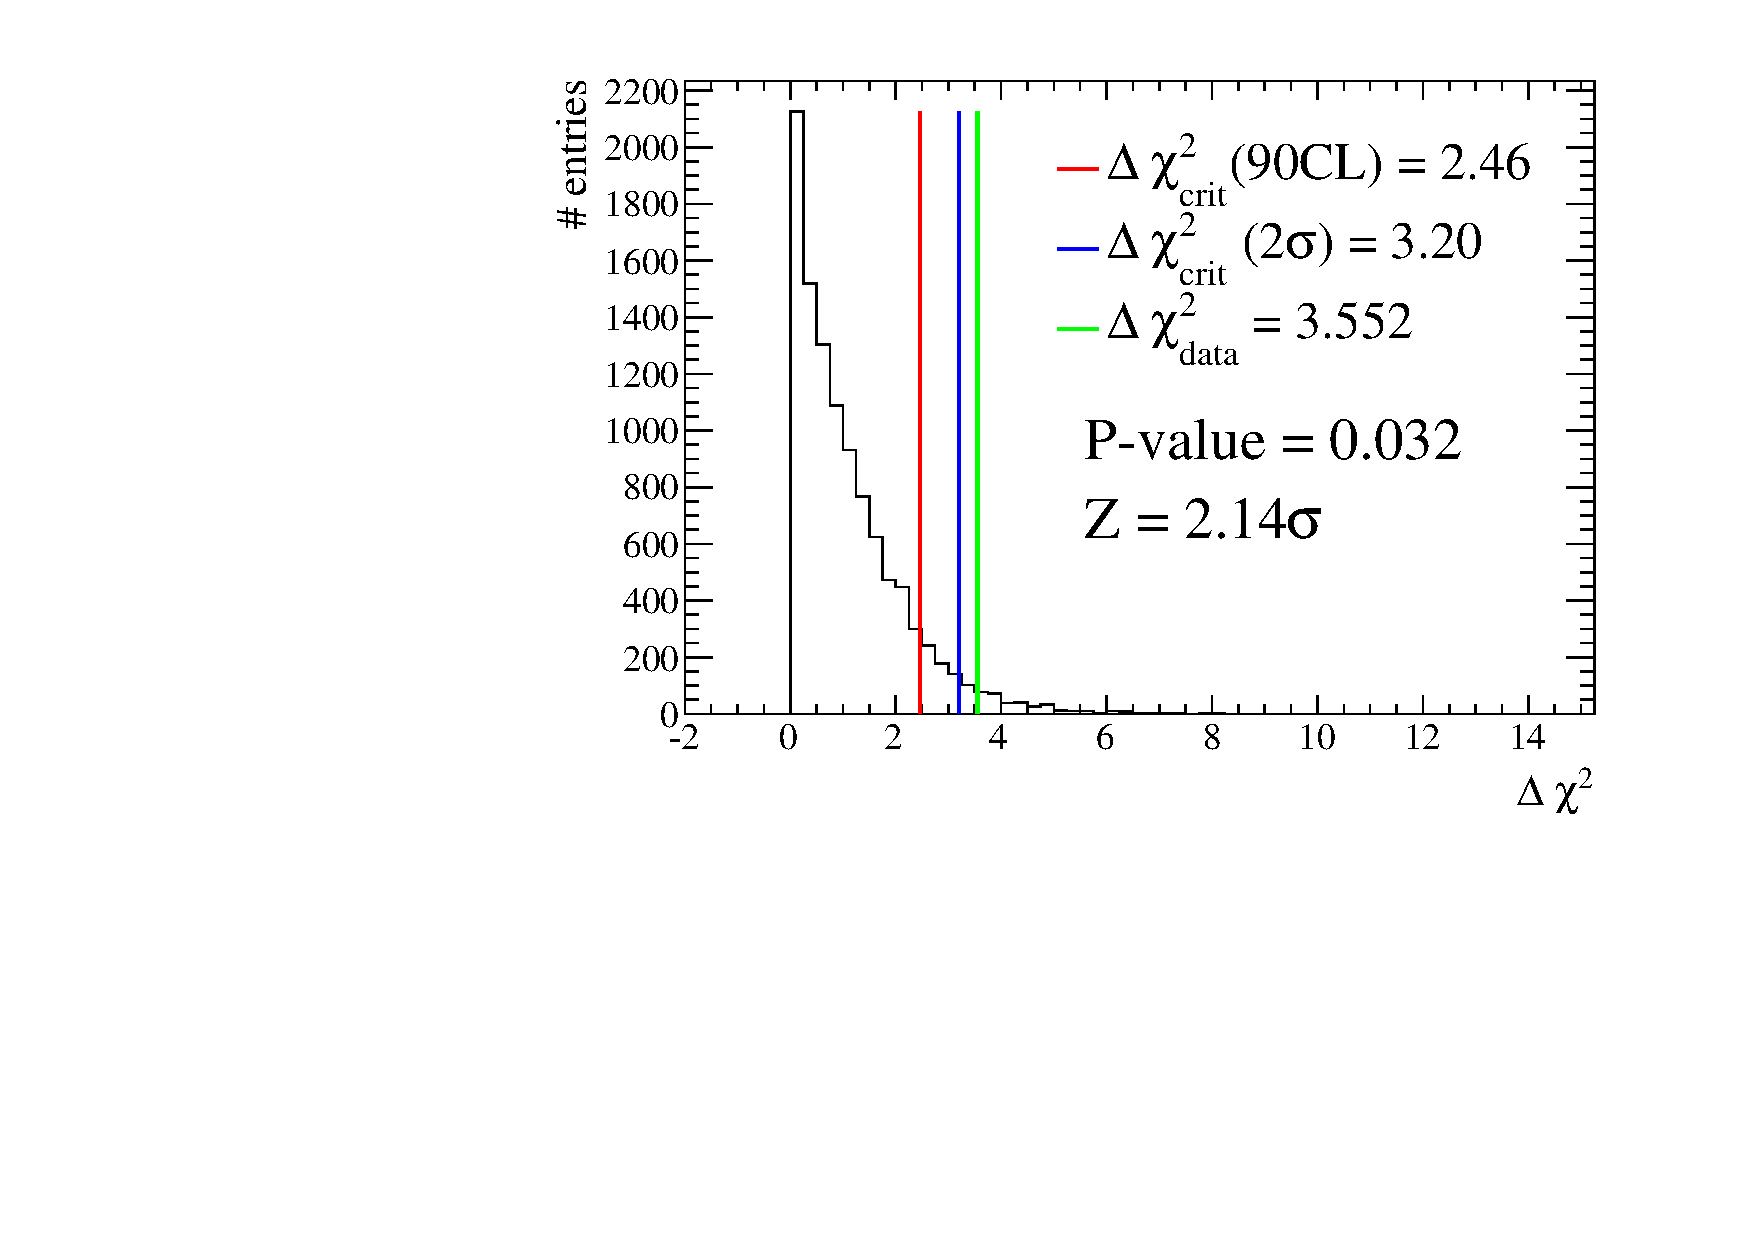
\includegraphics[width=0.49\textwidth]{joint_plots/coverage_fc/fc/significance_nh_dcp_0.pdf} 
\caption{
Distributions of $\Delta \chi^2$.  
$10k$ toy experiments are performed
with true values of $\delta_{CP} = 0$ (left) and $\pi$ (right), 
assuming normal hierarchy and applying the reactor constraint.
Both the mass hierarchy and $\delta_{CP}$ are profiled in the fit.
All the other oscillation parameters are marginalised.
The statistics corresponds to the Run 1-6 data set.
The $\Delta \chi^2$ value (green line) measured from the Run 1-6 data set
as well as the p-value and the significance as number of standard deviations (Z),
are shown as well.
}
\label{fig:joint_dcp_fc_example}
\end{figure*}

Then the significance can be shown as the number of standard deviations
where the measured quantity is assumed to be gaussian distributed.
In \cref{fig:zscore} the gaussian distribution of the measured variable $\mu$ is shown
as a function of the $Z$-score, i.e. how many standard deviations 
a certain measurement $x$ is far from the expected value:

\begin{equation}
Z = \frac{x-\mu}{\sigma}
\label{eq:zscore}
\end{equation}

If an experiment measures $x$,
$\alpha$ is the area of the p.d.f. corresponding to a certain CL (90\% in the example).
The quantity $\sigma$ is the bias of the measured value with respect to the expectation
 that contains $1-\alpha = 68.27\%$ of the total area.

The significance can be reported with the $Z$-score in the following way:

\begin{itemize}

\item the p-value is measured using \cref{eq:pvalue}

\item Assuming the p-value to be 1-sided (see \cref{fig:joint_dcp_fc_example}) and $\alpha$ 2-sided (see \cref{fig:zscore}), 
we set $\alpha = \text{p-value}$

\item $Z$, shown in \cref{eq:zscore}, is computed using the quantile distribution.
	Given the cumulative distribution function of the normal standard distribution with Mean=0 and RMS=1 ($\sigma=1$),
	
	\begin{equation}
	%\Phi(x) = \frac{1}{\sqrt{2\pi}} \int_{-\infty}^x e^{-t^2 / 2} dt, x \in [-x,x]
	%\Phi(x) = \frac{1}{\sqrt{2\pi}} \int_{Z \sigma}^{+\infty} e^{-t^2 / 2} dt = \alpha / 2  
	\Phi(x) = \frac{1}{\sqrt{2\pi}} \int_{Z}^{+\infty} e^{-t^2 / 2} dt = \alpha / 2  
	\label{eq:cumulative_norm}
	\end{equation}
		
%	Then 	
%	\begin{equation}
%	1 - \alpha  = 1 - 2 \Phi(x)
%	\label{eq:cumulative_norm}
%	\end{equation}
	
	the quantile is defined as
	
	\begin{equation}
	%Z = \Phi^{-1} (1 - \text{p-value})
	Z = \Phi^{-1} (1 - \alpha/2).
	\label{eq:quantile_norm}
	\end{equation}
	
	The ROOT function Math::gaussian\_quantile, that takes $\alpha$ as input, 
	and calculate the cumulative distribution function of the lower tail of the normal (Gaussian) distribution
	is defined as following:
	
	\begin{lstlisting}
	TF1 q("q","ROOT::Math::gaussian_quantile(1.-(x/2.)),1.)",0.,1.); 
  	double Zscore = q.Eval(pvalue); 
	\end{lstlisting}
	
\end{itemize} 


\begin{figure*}[htb]
\center
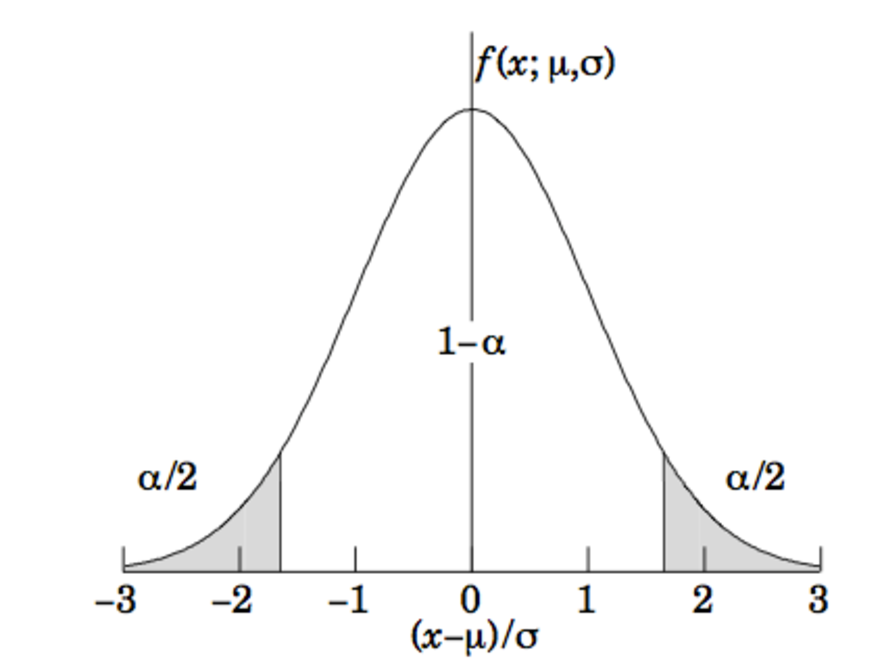
\includegraphics[width=0.49\textwidth]{joint_plots/coverage_fc/Zscore.pdf} 
\caption{
%Representation of  as a function of the Z-score.
 Illustration of a symmetric 90\% confidence interval (unshaded) 
 for a measurement of a single quantity with Gaussian errors. 
 Integrated probabilities, defined by $\alpha = 0.1$, are shown.}
\label{fig:zscore}
\end{figure*}


\clearpage




\end{appendices}

\clearpage

\end{document}


%%% Local Variables:
%%% mode: latex
%%% TeX-master: t
%%% End:
